\documentclass[spanish,12pt,a4paper]{book}
\usepackage{lmodern}
\usepackage[T1]{fontenc}
\usepackage{graphicx}

% Rutas relativas para las imagenes
\graphicspath{{imagenes/}}

\usepackage[utf8]{inputenc}
\usepackage[spanish]{babel}
\usepackage[
inner=2.5cm, outer=4.5cm,
top=3cm, bottom=3cm,
headheight=42pt,
marginparwidth=3.2cm, marginparsep=0.4cm
]{geometry}
\usepackage{fancyhdr}
%\usepackage[pages=all]{background}
\usepackage{longtable}
\usepackage{booktabs}
\usepackage{array}
\usepackage{colortbl}
\usepackage{hyperref}
\usepackage{makecell}
\usepackage{ragged2e}
\usepackage{needspace}
\usepackage[
type={CC},
modifier={by-nc-sa},
version={4.0},
lang={spanish}
]{doclicense}
\usepackage[dvipsnames,svgnames,x11names]{xcolor}
\usepackage{marginnote}       % Notas marginales (§6 Manual de Estilo)
% --- Estilo de marginnote (§6 del Manual de Estilo) ---
\renewcommand*{\marginfont}{\footnotesize\sffamily\color{plapaAzul!85}}
\renewcommand*{\raggedleftmarginnote}{\RaggedLeft}
\renewcommand*{\raggedrightmarginnote}{\RaggedRight}


\usepackage{microtype}        % Mejora tipográfica: tracking, kerning
% Comando para guardar el subtítulo de cada Parte
\newcommand{\partsubtitlestore}{}
\newcommand{\partsubtitle}[1]{\renewcommand{\partsubtitlestore}{#1}}
% partmark (legacy) ahora delega en partsubtitle (solo \providecommand)
\providecommand{\partmark}[1]{\partsubtitle{#1}}
\usepackage{enumitem}
\usepackage{tikz}
\usepackage{titlesec}        % Estilizado de \part, \chapter, \section
\usepackage[most]{tcolorbox}
\usepackage{emptypage}


\setlength{\extrarowheight}{4pt}



\hyphenation{
	Neu-ro-plas-ti-ci-dad
	Res-pon-sa-bi-li-dad
	Tra-ves-ti-Trans
	Co-mor-bi-li-dad
	Pro-ta-go-nis-mo
	Dis-cer-ni-mien-to
	Psi-co-ac-ti-va
	%He-ma-to-en-ce-fá-li-ca
	%bu-ro-crá-ti-cos
	ins-ti-tu-cio-nal
	Tras-cen-den-cia
	%A-com-pa-ña-mien-to
	%Nar-co-trá-fi-co
	Mi-se-ri-cor-dia
	Pro-ta-go-nis-mo
	Res-pon-sa-bi-li-dad
	Au-to-cui-da-do
}

\hypersetup{
	hidelinks,
	pdfborder={0 0 0},
	pdftitle={Manual de la PLAPA},
	pdfauthor={PLAPA -- CELAM},
	pdfsubject={Pastoral Latinoamericana de Acompañamiento y Prevención de las Adicciones},
	pdfkeywords={pastoral, adicciones, CELAM, PLAPA, Ver-Juzgar-Actuar},
	pdfcreator={LaTeX},
}

% Para el índice temático
\usepackage{imakeidx}
\makeindex[title=Índice temático, columns=2]


% --- Paquetes adicionales para Tablas ---
\usepackage{calc}         % Soluciona: \real 
\usepackage{etoolbox}     % Ayuda con parches internos de tablas

\pagestyle{fancy}
\fancyhf{}
\fancyhead[L]{\small\sffamily\textcolor{plapaAzul}{Manual de PLAPA}}
% \fancyhead[C] eliminado: el logo se superponía con \leftmark (§5 minimalismo)
\fancyhead[R]{\small\sffamily\textcolor{plapaAzul!70}{\leftmark}}
\fancyfoot[C]{\small\sffamily\textcolor{plapaAzul}{\thepage}}
\renewcommand{\footrulewidth}{0pt}
% Línea fina dorada bajo el encabezado (vía \headrule customizado)
\renewcommand{\headrule}{\hbox to\headwidth{\color{plapaDorado}\leaders\hrule height 0.5pt\hfill}}
\renewcommand{\headrulewidth}{0.5pt}

%\backgroundsetup{
	%	scale=1,            % Escala de la imagen (1 = tamaño original)
	%	color=black,        % No afecta si es una imagen, pero se define por defecto
	%	opacity=0.5,          % Opacidad (1 es total, 0.5 es semitransparente)
	%	angle=0,            % Rotación
	%	contents={%
		%		
		
		% Esto es vital para que las listas no den error
		\providecommand{\tightlist}{%
			\setlength{\itemsep}{0pt}\setlength{\parskip}{0pt}}
		
		
		
		% Definición del estilo de la ficha de propuestas
		\newtcolorbox{fichalateral}{
			colback=gray!15,            % Fondo blanco (o gray!5 si querés un gris sutil)
			colframe=black!70,         % Color de la línea de la izquierda
			boxrule=0pt,              % Elimina todos los bordes tradicionales
			leftrule=3pt,             % Aplica un borde grueso solo a la izquierda
			sharp corners,            % Esquinas completamente rectas tipo "callout"
			width=0.95\textwidth,      % Ancho del recuadro
			left=4mm, right=4mm,       % Márgenes internos horizontales
			top=2mm, bottom=2mm,       % Márgenes internos verticales
			before=\noindent\centering % Asegura el centrado del bloque
		}
		
		% =====================================================================
		% ENTORNOS DEL MANUAL DE ESTILO PLAPA (CELAM)
		% =====================================================================
		
		% --- Paleta de colores PLAPA ---
		\definecolor{plapaAzul}{HTML}{1B3A5C}       % Azul institucional CELAM
		\definecolor{plapaDorado}{HTML}{C5A028}      % Dorado (acentos litúrgicos)
		\definecolor{plapaRojo}{HTML}{8B1A1A}        % Rojo oscuro (alertas pastorales)
		\definecolor{plapaVerde}{HTML}{2E5939}       % Verde (esperanza, Actuar)
		\definecolor{plapaGris}{HTML}{F5F5F0}        % Gris cálido (fondos)
		\definecolor{plapaCrema}{HTML}{FAF7F0}       % Crema (fondo de cajas)
		
		% --- Caja de Resonancia (§8 del Manual de Estilo) ---
		% Para testimonios territoriales y frases de alto impacto emocional.
		% La vivencia sufriente sea lo primero que se retenga en un hojeado rápido."
		\newtcolorbox{cajaResonancia}[1][]{%
			colback=plapaCrema,
			colframe=plapaDorado,
			boxrule=0pt,
			leftrule=4pt,
			rightrule=0pt,
			toprule=0pt,
			bottomrule=0pt,
			sharp corners,
			width=0.92\textwidth,
			left=6mm, right=6mm,
			top=4mm, bottom=4mm,
			fontupper=\itshape,
			before=\par\medskip\noindent\centering,
			after=\par\medskip,
			#1
		}
		
		% --- Alerta Pastoral / "Curva Peligrosa" (§8 del Manual de Estilo) ---
		% Para párrafos de discernimiento teológico profundo o situaciones 
		% pastorales complejas que requieren una pausa obligatoria en la lectura.
		\newtcolorbox{alertaPastoral}[1][]{%
			colback=white,
			colframe=plapaRojo,
			boxrule=0pt,
			leftrule=4pt,
			sharp corners,
			width=0.95\textwidth,
			left=5mm, right=4mm,
			top=3mm, bottom=3mm,
			title={\textbf{\textcolor{plapaRojo}{\Cross\enspace Discernimiento pastoral}}},
			coltitle=plapaRojo,
			fonttitle=\bfseries\small,
			colbacktitle=white,
			boxed title style={boxrule=0pt, colframe=white},
			before=\par\medskip\noindent\centering,
			after=\par\medskip,
			#1
		}
		
		% --- Caja de Criterio de Discernimiento (§3 - Estructura Escolástica) ---
		\newtcolorbox{criterioDiscernimiento}[1][]{%
			colback=plapaGris,
			colframe=plapaAzul,
			boxrule=0.5pt,
			arc=0pt,
			width=0.95\textwidth,
			left=4mm, right=4mm,
			top=3mm, bottom=3mm,
			before=\par\medskip\noindent\centering,
			after=\par\medskip,
			#1
		}
		
		% --- Caja para citas del Magisterio (§3) ---
		\newtcolorbox{citaMagisterio}[1][]{%
			colback=white,
			colframe=plapaAzul!40,
			boxrule=0pt,
			leftrule=3pt,
			sharp corners,
			width=0.90\textwidth,
			left=5mm, right=5mm,
			top=3mm, bottom=3mm,
			fontupper=\small\itshape,
			before=\par\smallskip\noindent\centering,
			after=\par\smallskip,
			#1
		}
		
		
		% =====================================================================
		% ESTILIZADO DE ENCABEZADOS (titlesec) — Manual de Estilo §3, §5
		% Tipografía al servicio del encuentro: minimalismo, jerarquía clara.
		% =====================================================================
		
		% --- \part: pantalla casi en blanco, número grande en plapaAzul ---
		\titleformat{\part}[display]
		{\centering\normalfont\sffamily}
		{\fontsize{30}{36}\selectfont\textcolor{plapaDorado}{\textsc{Parte \thepart}}}
		{1.5em}
		{\fontsize{42}{50}\selectfont\bfseries\textcolor{plapaAzul}}
		[%
		\ifdefempty{\partsubtitlestore}{}{%
			\vskip 0.5em
			\centerline{\Large\sffamily\itshape\color{plapaAzul!70}\partsubtitlestore}%
			\global\renewcommand{\partsubtitlestore}{}%
		}%
		\vskip 1em
		\centerline{\textcolor{plapaDorado}{\rule{0.4\textwidth}{1.5pt}}}%
		]
		
		% --- \chapter: número en plapaDorado, título en plapaAzul ---
		\titleformat{\chapter}[display]
		{\normalfont\sffamily}
		{\fontsize{20}{24}\selectfont\textcolor{plapaDorado}{\textsc{Capítulo \thechapter}}}
		{0.8em}
		{\fontsize{26}{32}\selectfont\bfseries\textcolor{plapaAzul}}
		[\vspace{0.5em}{\color{plapaDorado}\rule{0.25\textwidth}{1pt}}]
		
		% --- \chapter* (sin numerar): solo título coloreado ---
		\titleformat{name=\chapter,numberless}[display]
		{\normalfont\sffamily}
		{}
		{0pt}
		{\fontsize{26}{32}\selectfont\bfseries\textcolor{plapaAzul}}
		[\vspace{0.5em}{\color{plapaDorado}\rule{0.25\textwidth}{1pt}}]
		
		% --- \section: línea acento a la izquierda + título en plapaAzul ---
		\titleformat{\section}
		{\normalfont\Large\bfseries\sffamily\color{plapaAzul}}
		{\textcolor{plapaDorado}{\thesection}\hspace{0.5em}|\hspace{0.5em}}
		{0pt}
		{}
		
		% --- \subsection: en plapaAzul más sobrio ---
		\titleformat{\subsection}
		{\normalfont\large\bfseries\sffamily\color{plapaAzul!85}}
		{\textcolor{plapaDorado!90}{\thesubsection}\hspace{0.6em}}
		{0pt}
		{}
		
		% --- Espaciado de encabezados (más aire — §5 "página debe respirar") ---
		\titlespacing*{\section}{0pt}{2.5ex plus 1ex minus .2ex}{1.5ex plus .2ex}
		\titlespacing*{\subsection}{0pt}{2ex plus 1ex minus .2ex}{1ex plus .2ex}
		
		% --- Símbolo de cruz para alertas pastorales ---
		\newcommand{\Cross}{$\dagger$}
		
		% --- Método escolástico (§3 del Manual de Estilo) ---
		% \momento{Planteo del tema} → encabezado azul sans-serif para los 6 momentos
		% del método: Planteo, Pregunta, Objeciones, Fundamento, Tesis, Respuesta.
		\newcommand{\momento}[1]{%
			\needspace{4\baselineskip}
			\par\medskip\noindent
			{\sffamily\bfseries\large\color{plapaAzul}%
				{\color{plapaDorado}\rule[0.15ex]{0.6em}{0.6em}}~#1}%
			\par\nobreak\smallskip\noindent\ignorespaces
		}
		
		% Sub-momento para Objeción 1/2/3 y A la primera/segunda/tercera
		\newcommand{\submomento}[1]{%
			\par\smallskip\noindent
			{\sffamily\bfseries\color{plapaAzul!85}#1}\ %
		}
		
		
		
		
		
		
		
		
		
		% --- Estilizado del Índice (\tableofcontents) ---
		\usepackage{tocloft}
		\renewcommand{\cftpartfont}{\sffamily\bfseries\large\color{plapaAzul}}
		\renewcommand{\cftchapfont}{\sffamily\bfseries\color{plapaAzul}}
		\renewcommand{\cftsecfont}{\sffamily\color{plapaAzul!85}}
		\renewcommand{\cftsubsecfont}{\sffamily\color{plapaAzul!75}}
		\renewcommand{\cftpartpagefont}{\bfseries\color{plapaDorado}}
		\renewcommand{\cftchappagefont}{\color{plapaDorado}}
		\renewcommand{\cftsecpagefont}{\color{plapaDorado!90}}
		
		% --- Tipografía: respiración y legibilidad (§5, §7 del Manual de Estilo) ---
		\linespread{1.15}              % Interlineado ligeramente más amplio
		\setlength{\parskip}{0.6em}     % Espacio entre párrafos (aire)
		\setlength{\parindent}{0pt}     % Sin sangría (estilo moderno)
		\setlength{\emergencystretch}{3em} % Evita Overfull \hbox
		
		\title{Manual de la PLAPA}  % Solo para metadatos PDF (hyperref)
		\author{PLAPA -- CELAM}
		\date{26 de Junio de 2026}
		
		% --- Redefinición de la Portada para que ocupe TODA la página (Sin bordes blancos) ---
		\usepackage{environ}
		\RenewEnviron{titlepage}{%
			\clearpage
			\thispagestyle{empty}
			\begin{tikzpicture}[remember picture, overlay]
				\node[inner sep=0pt, line width=0pt] at (current page.center) {%
					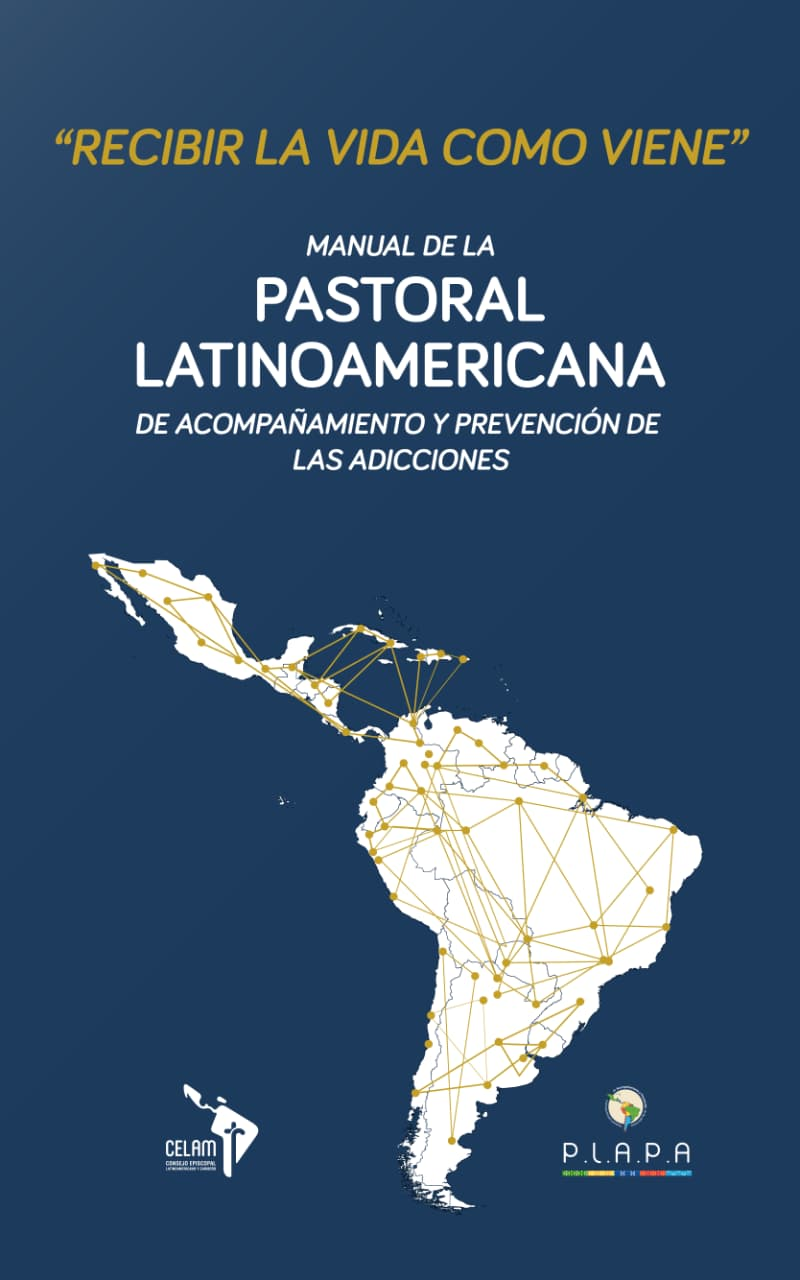
\includegraphics[width=\paperwidth, height=\paperheight]{tapa-manual.jpeg}%
				};
			\end{tikzpicture}
			\clearpage
		}



\begin{document}

	% =================================================================
	% PORTADA (titlepage explícita — Manual de Estilo §5, §6)
	% Una sola página, centrada, sin encabezado ni número de página.
	% =================================================================
	\begin{titlepage}
		\thispagestyle{empty}
		\centering
		\setlength{\parskip}{0pt}
		
		\vspace*{\fill}
		
		{\color{plapaDorado}\rule{0.5\textwidth}{1.5pt}}
		
		\vspace{1.5em}
		
		{\fontsize{40}{48}\selectfont\sffamily\bfseries\textcolor{plapaAzul}{Manual de la PLAPA}}
		
		\vspace{1.2em}
		
		{\Large\sffamily\textcolor{plapaAzul!70}{Pastoral Latinoamericana de Acompañamiento\\y Prevención de las Adicciones}}
		
		\vspace{1.2em}
		
		{\color{plapaDorado}\rule{0.5\textwidth}{1.5pt}}
		
		\vspace{3em}
		
		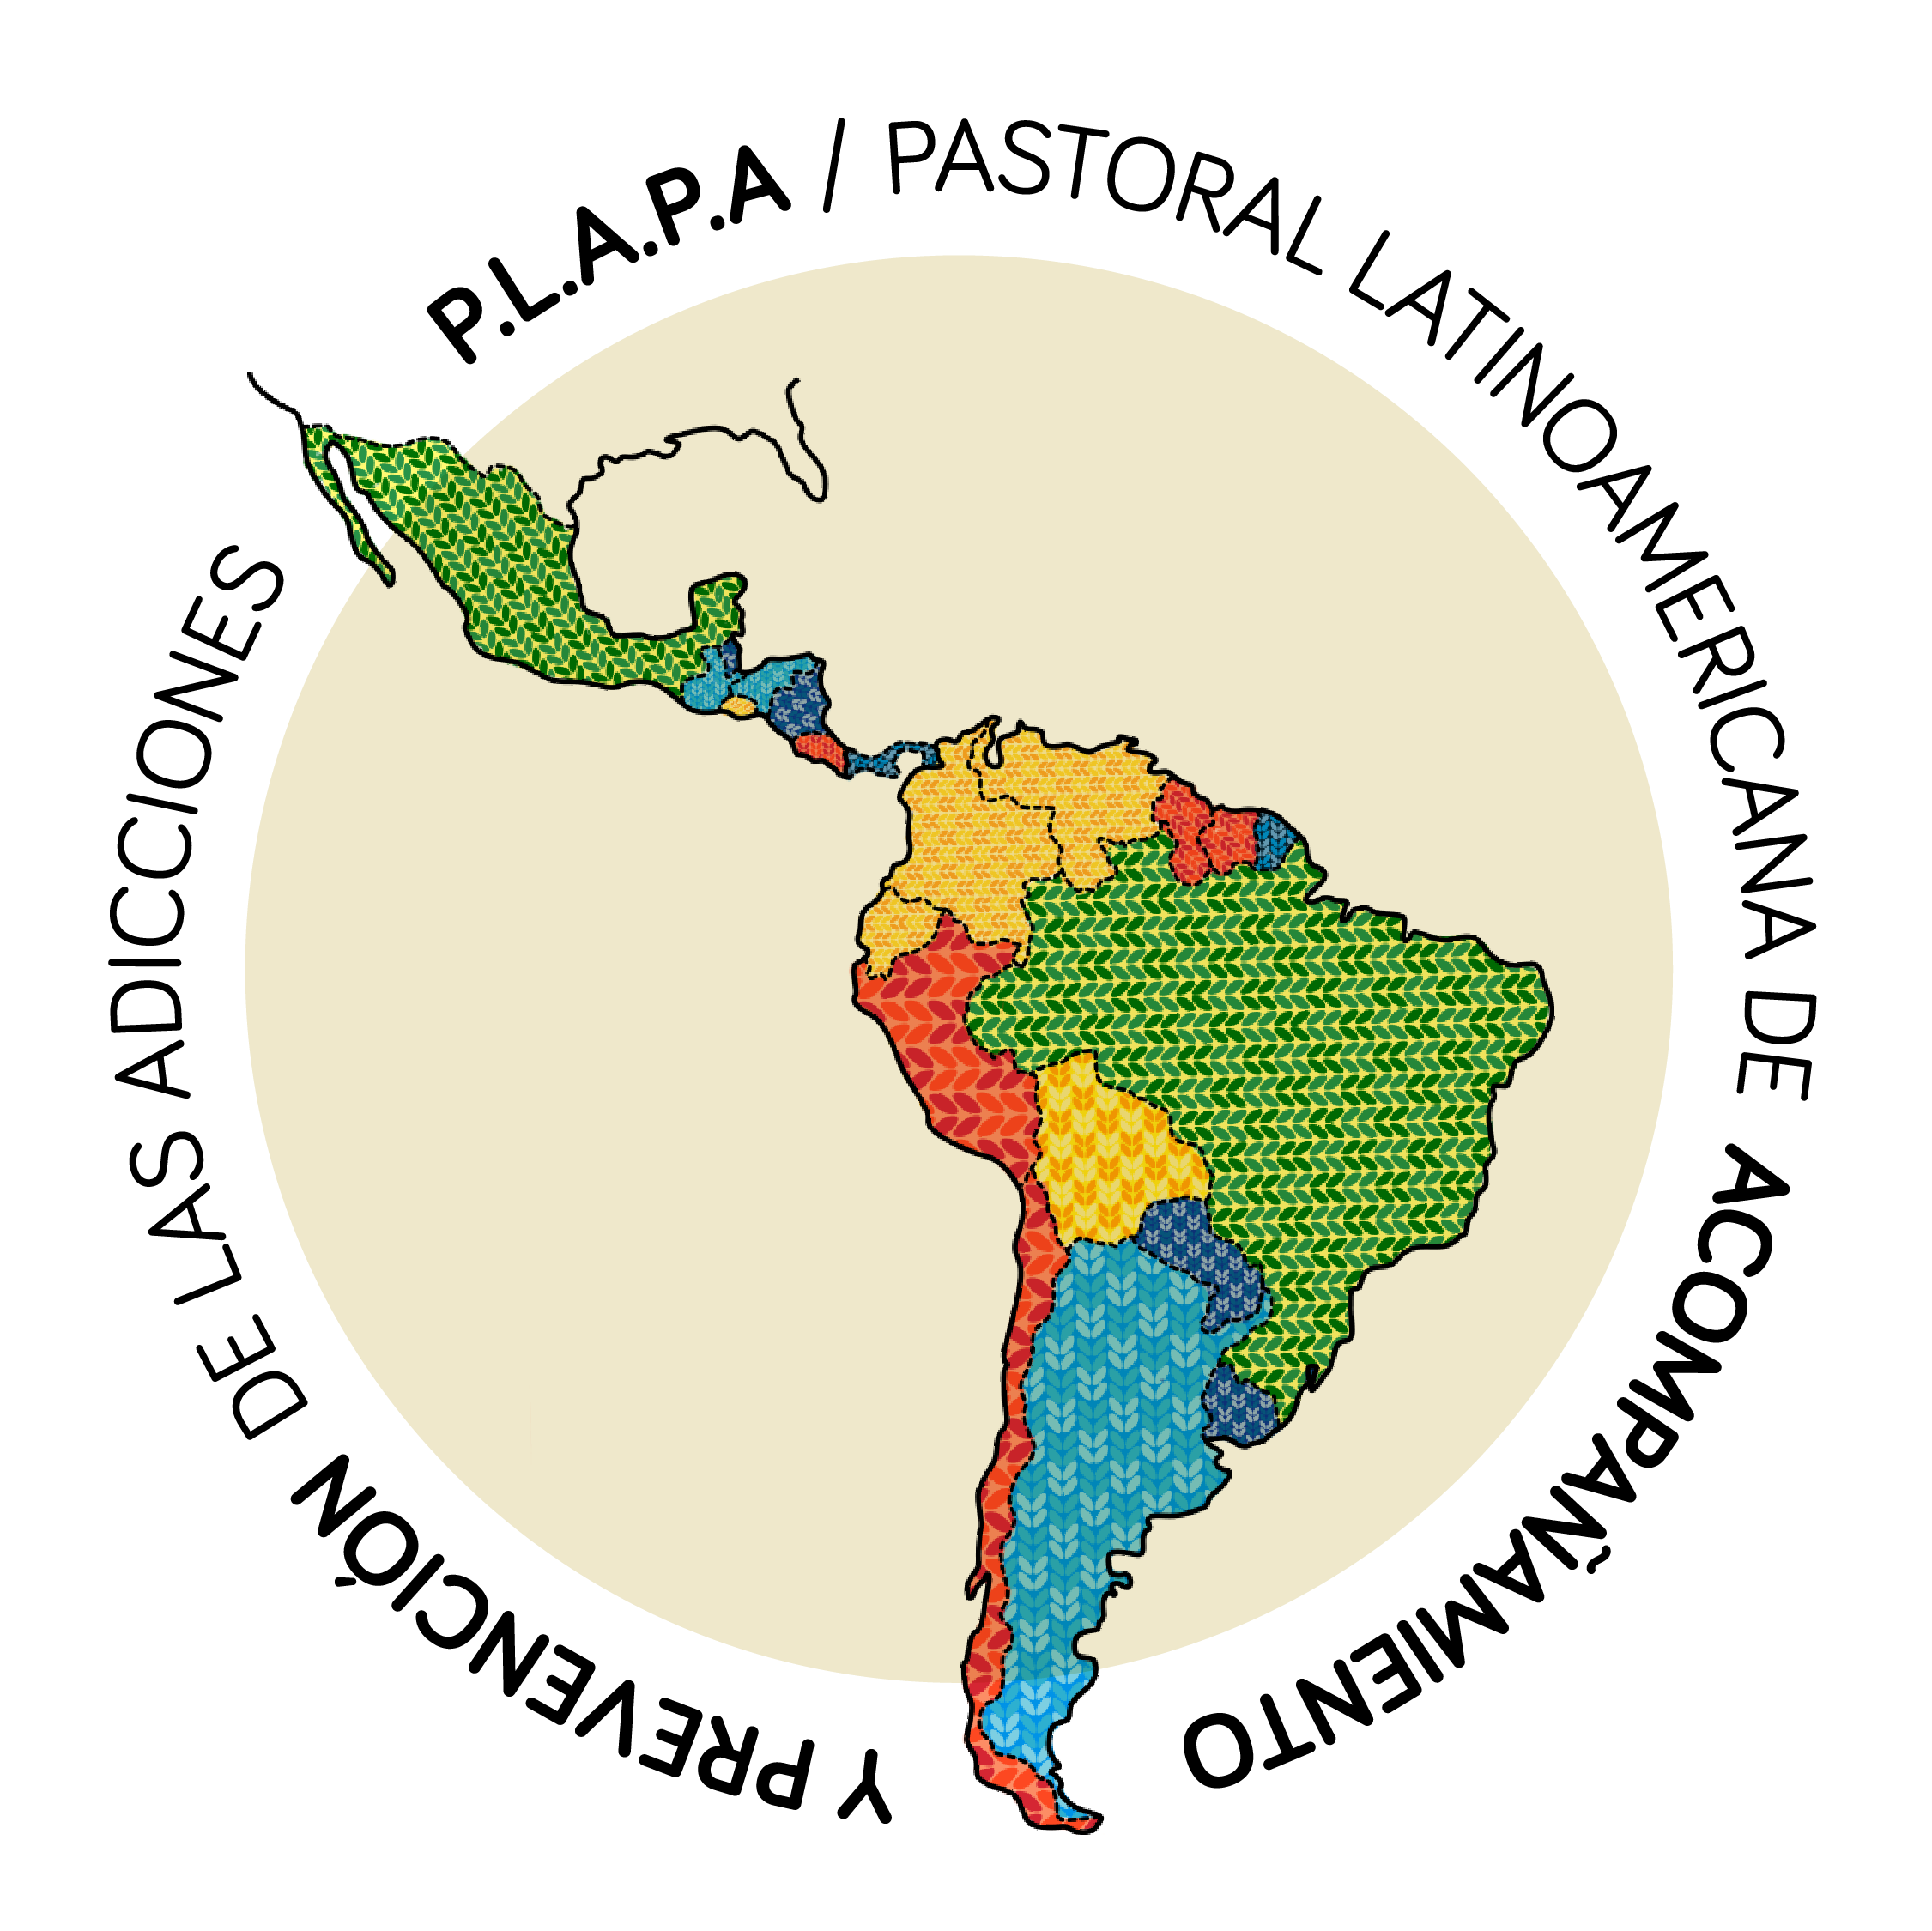
\includegraphics[scale=0.4]{PLAPA-LOGO.png}
		
		\vfill
		
		{\Large\sffamily\textcolor{plapaAzul!70}{26 de junio de 2026}}
		
		\vspace*{\fill}
	\end{titlepage}
	
	% ── PÁGINA LEGAL ──
	\thispagestyle{empty}
	
	
	{\small
	
	Con las debidas licencias eclesiásticas. Reservados todos los derechos. Esta publicación no puede ser reproducida ni en todo ni en parte por cualquier medio sin el permiso previo por escrito del CELAM 
	
	© Consejo Episcopal Latinoamericano y Caribeño CELAM\\Avenida Boyacá N.° 169D-75\\Código postal 111166\\PBX: 601 484 5804\\celam@celam.org\\www.celam.org\\Bogotá, D. C., 2026.
	
	
	\bigskip
	
	% 1. EDICIÓN
	Primera edición: junio de 2026.
	
	\medskip
	
	% 2. CIUDAD
	Bogotá, Colombia.
	
	\medskip
	
	% 3. COORDINACIÓN (vos)
	\textbf{Coordinación general:} Pbro. Carlos Olivero.
	
	\medskip
	
	% 4. EQUIPO CURADOR (el que anunciás en 13.6)
	% \textbf{Equipo curador:} [Nombre 1], [Nombre 2], [Nombre 3].
	
	% \medskip
	
	% 5. DISEÑO Y DIAGRAMACIÓN
	\textbf{Diseño y diagramación:} [«Equipo PLAPA»].
	
	\medskip
	
	% 6. ILUSTRACIONES
	\textbf{Ilustraciones:} \textbf{Ilustraciones:} Generadas mediante DALL-E (OpenAI) y editadas por el equipo de la PLAPA. La imagen del Retablo de Isenheim (Figura~3.1) es de dominio público.
	
	\medskip
	
	% 7. ISBN (si lo tramitás)
	% ISBN: 978-XXX-XXXX-XX-X
	
	% 8. DEPÓSITO LEGAL (si aplica en Colombia)
	% Depósito legal: XXXXX
	
	\medskip
	
	% 9. CONTACTO
	\textbf{Contacto:} [info@plapa.org]
	
	
	
	\doclicenseThis
	
	\medskip
	
	
	}
	
	\newpage
	\tableofcontents
	
	
	\partsubtitle{Cómo nace este manual}
	\part{El punto de partida}
	
	\chapter{Puerta de entrada}
	
	\section{Presentación}
	
	Este Manual de Pastoral de Adicciones nace del clamor de nuestros pueblos y del compromiso de una Iglesia que, en América Latina y el Caribe, ha decidido no mirar para otro lado frente al sufrimiento provocado por el consumo de sustancias psicoactivas. Es fruto de un camino eclesial compartido, marcado por la escucha\index{escucha} de la realidad y el discernimiento comunitario, en diálogo permanente con las experiencias pastorales que acompañan la vida herida de personas, familias y comunidades.
	
	El fenómeno del consumo de sustancias psicoactivas constituye hoy una de las expresiones más dolorosas de la exclusión social. Tal como lo expresó el Documento de Aparecida\label{apar}, se trata de una realidad que se expande como una “mancha de aceite”, afectando de modo particular a los sectores más pobres y vulnerables. No estamos ante un problema meramente individual ni exclusivamente sanitario, sino frente a una herida social y cultural que interpela de manera directa la misión evangelizadora de la Iglesia.
	
	En este contexto, la Iglesia latinoamericana ha ido desarrollando diversas respuestas pastorales orientadas a prevenir, acompañar y reconstruir vidas desde una mirada integral. Este Manual recoge ese camino eclesial, valorando especialmente las experiencias que nacen en las comunidades y que, muchas veces con escasos recursos, sostienen procesos de cuidado, acompañamiento y esperanza. No es un texto elaborado desde un escritorio, sino una herramienta que brota del contacto con la realidad y de una reflexión pastoral que nace desde el pueblo y con el pueblo, en continuidad con la tradición teológica latinoamericana promovida desde el CELAM. 
	
	Este Manual se inscribe explícitamente en el camino de la Pastoral Latinoamericana de las Adicciones PLAPA, impulsada desde el CELAM como un espacio de discernimiento y unidad pastoral frente a esta realidad compleja. En sintonía con el documento fundante de la PLAPA\label{docp}, y con la  Carta a la Iglesia de América Latina y el Caribe\label{cial}, se asume una mirada integral, comunitaria y territorial, que pone en el centro la dignidad de la persona y promueve el trabajo en red con otros actores sociales.
	
	El proceso de elaboración de este Manual se desarrolló en clave sinodal\index{sinodalidad}, a partir del aporte de agentes pastorales, equipos territoriales, consagradas y consagrados, sacerdotes, obispos y profesionales comprometidos. El resultado no pretende ofrecer respuestas cerradas ni modelos únicos, sino compartir criterios y orientaciones pastorales que ayuden a acompañar procesos de vida en contextos diversos.
	
	Este Manual está destinado a comunidades parroquiales, escuelas católicas, diócesis, movimientos y organizaciones eclesiales que desean involucrarse —o seguir profundizando— en la prevención y el acompañamiento de personas en situación de consumo. Quiere ser un apoyo para la formación de agentes y la revisión de prácticas pastorales, evitando tanto el moralismo como la ingenuidad, y poniendo siempre en el centro la dignidad de la persona humana.
	
	Conviene aclarar que este Manual, aunque intenta poner en diálogo los aportes de la ciencia y de la fe, no es un protocolo clínico ni un instrumento técnico especializado. Tampoco pretende sustituir los aportes de las ciencias de la salud ni la responsabilidad irrenunciable de los Estados en el diseño e implementación de políticas públicas. Su aporte específico es pastoral: ofrecer un horizonte evangelizador y animar prácticas concretas de cuidado y acompañamiento comunitario.
	
	\section{\textquestiondown Cómo utilizar este manual?}
	
	El presente manual ha sido concebido no solo como un documento teórico, sino como una herramienta viva y dinámica para el acompañamiento\index{acompañamiento} en el ámbito de las adicciones y la vulnerabilidad social por parte de la Iglesia. Por su naturaleza, este material ofrece dos modalidades de lectura complementarias, adaptándose a los tiempos y necesidades de cada comunidad o agente pastoral.
	
	\begin{itemize}
		\item En primer lugar, el manual puede ser leído de manera lineal, de principio a fin, como un libro de texto. Esta modalidad permite una comprensión profunda y sistemática de la propuesta, recorriendo el camino lógico que va desde el análisis de la realidad hasta la implementación de respuestas concretas. Es el camino ideal para quienes se inician en esta pastoral o desean fundamentar su práctica desde una base teórica sólida. 
		
		\item En segundo lugar, el manual está diseñado para ser consultado en función de las necesidades y preguntas emergentes. Entendemos que la labor en el territorio es urgente y que, a menudo, el agente pastoral se encuentra frente a desafíos específicos que requieren respuestas inmediatas. Por ello, el material funciona como un recurso de consulta rápida, donde se pueden buscar secciones específicas según la problemática que se esté enfrentando en el momento. La versión virtual del manual ofrece buenas oportunidades en este sentido.
	\end{itemize}
	
	La flexibilidad que proponemos se refleja directamente en la estructura metodológica que realizamos para la elaboración, y quedó consignada en las tres grandes partes del manual:
	
	\begin{enumerate}
		\item \textbf{Recibir la Realidad (Ver):} Aquí se sistematiza la mirada de los distintos agentes pastorales de nuestra región. No es una descripción abstracta, sino el reflejo de lo que nuestros hermanos y hermanas están viendo hoy en los barrios, las parroquias y los centros de acompañamiento. Es el punto de partida necesario para situar nuestra acción.
		\item \textbf{El Discernimiento (Juzgar):} Esta\index{discernimiento|textbf} sección es el corazón teórico del manual y está construida íntegramente en función de las preguntas que surgen en el corazón y en la práctica de un agente pastoral. En lugar de ofrecer verdades cerradas, proponemos un camino de reflexión que ayuda a iluminar la realidad desde nuestra fe y nuestro compromiso social, respondiendo a los interrogantes que la práctica cotidiana nos plantea.
		\item \textbf{La Respuesta (Actuar):} Aquí presentamos propuestas concretas de intervención. Son líneas de acción probadas y sugerencias prácticas para transformar la realidad observada en la Parte 1 (Ver), a la luz del discernimiento realizado en la Parte 2 (Juzgar).
	\end{enumerate}
	
	Finalmente, conscientes de que la problemática de las adicciones requiere un abordaje integral, hemos incorporado en la versión virtual un sistema de hipervínculos que relacionan los contenidos entre sí. Esta red de conexiones permite que el lector no vea los temas como compartimentos estancos, sino como dimensiones interconectadas de una misma realidad. Al hacer clic en estos vínculos, se podrá navegar entre conceptos, herramientas y testimonios, favoreciendo una visión de conjunto que es indispensable para una respuesta pastoral que aspire a la integralidad\index{integralidad}. 
	
	Por último, este manual aspira a ser un material \textit{rolling release}, es decir, en actualización continua, de manera tal que desde la PLAPA implementaremos los mecanismos para la participación activa, que como se comprenderá, se reflejará actualizada siempre antes en la versión digital. A tal efecto, crearemos un equipo encargado de evaluar e incorporar las correcciones de la comunidad. 
	
	Esperamos que este manual sea un compañero de camino que fortalezca la esperanza y la eficacia de nuestra misión en el territorio.
		
	\section{Prólogo}
	
	\begin{citaMagisterio}
		El problema de la droga es como una mancha de aceite que invade todo. No reconoce fronteras, ni geográficas ni humanas. Ataca por igual a países ricos y pobres, a niños, jóvenes, adultos y ancianos, a hombres y mujeres. La Iglesia no puede permanecer indiferente ante este flagelo que está destruyendo a la humanidad, especialmente a las nuevas generaciones. Su labor se dirige especialmente en tres direcciones: prevención, acompañamiento y sostén de las políticas gubernamentales para reprimir esta pandemia.
		
		\raggedleft
		\textbf{\textcolor{plapaAzul}{Documento de Aparecida}} N° 422\label{aparb}
	\end{citaMagisterio}
	
	
	Con estas palabras, ya en 2007, nuestros pastores señalaban la necesidad de que la Iglesia se involucre en el problema de la droga. \textit{La Iglesia no puede permanecer indiferente}, decían. Casi 20 años después constatamos con dolor que el problema se profundizó, y que en la Iglesia nos cuesta mucho involucrarnos. 
	
	Pareciera que meterse en el problema de la droga es meterse en el terreno de los especialistas; que se trata de un tema muy complejo y que nosotros no tenemos nada que aportar. Pareciera que es un asunto reservado a algunas personas llamadas de un modo particular o que descubrieron esa vocación específica, pero que en general nuestras comunidades no tienen nada que hacer. 
	
	Nosotros no pensamos así, y esa es la razón por la que nos embarcamos en la difícil tarea de escribir este manual. Queremos decir que nuestras comunidades, parroquias, escuelas y pastorales tienen muchísimo para aportar, y que hay cosas que si no hacemos nosotros, nadie más las hará. Que el dolor y la muerte que traen las sustancias psicoactivas son una ocasión privilegiada para encontrar al crucificado, y que en ese lugar se descubre la resurrección. Incluso queremos aventurarnos a decir, que en la apertura que tengamos a las llagas de la sociedad, se juega nuestra salvación, porque en esas heridas habita el mismo Jesucristo.  
	
	Decía el Papa Francisco: 
	
	\begin{citaMagisterio}
		A veces sentimos la tentación de ser cristianos manteniendo una prudente distancia de las llagas del Señor. Pero Jesús quiere que toquemos la miseria humana, que toquemos la carne sufriente de los demás. Espera que renunciemos a buscar esos cobertizos personales o comunitarios que nos permiten mantenernos a distancia del nudo de la tormenta humana, para que aceptemos de verdad entrar en contacto con la existencia concreta de los otros y conozcamos la fuerza de la ternura. Cuando lo hacemos, la vida siempre se nos complica maravillosamente y vivimos la intensa experiencia de ser pueblo, la experiencia de pertenecer a un pueblo.
		
		\raggedleft
		\textbf{\textcolor{plapaAzul}{Evangelii Gaudium\label{FEG}}} N° 270
	\end{citaMagisterio}
	
	
	
	El problema de la droga y la adicción de nuestros hermanos, sin lugar a dudas es una de esas llagas del Señor que señalaba el Papa Francisco. A veces nos puede dar miedo, o inseguridad. Tiene tantos elementos que considerar, que pareciera difícil meterse y hacer las cosas bien. Sin embargo, la Iglesia nos llama a comprometernos. 
	
	Por eso es importante decir: La Iglesia no se mete en este tema con la lógica de la eficacia. La relación de los cristianos con los enfermos no es igual que la relación del médico. El médico se relaciona para tratar y curar, o en su defecto hacer más llevadero el dolor. La Iglesia, aunque quiere ayudar a las personas a superar aquellos males que las aquejan, en su modo de acompañar, orar, y estar al lado amorosamente descubre que la lógica de la eficacia enmudece junto a la cruz, para dar lugar a un modo de estar más profundo. Es lo que vimos en la escena de la crucifixión:  \textit{uno de los malhechores colgados le insultaba:  ¿No eres tú el Cristo? Pues ¡sálvate a ti y a nosotros!} (Lc 23, 39\label{lc23.39}). El pobre había escuchado tanto sobre las curaciones milagrosas y los signos que Jesús había realizado, que llegó incluso desde su enojo a exigírselo. Hubiera querido que ese encuentro con Jesús crucificado se tradujera rápidamente en términos de eficacia. Sin embargo no era ese el camino que estaba invitado a transitar. El otro ladrón lo entendió, y en su apertura logró encontrar el consuelo: \textit{Te aseguro que hoy estarás conmigo en el Paraíso.} (Lc 23, 43).
	
	Nosotros siempre queremos que las personas se recuperen, que las familias se sanen, que nuestras comunidades sean espacios seguros y nuestros colegios libres de problemas. Pero no siempre logramos alcanzar esas metas. Lo importante es descubrir la luz en el camino, que es la que alimenta nuestra esperanza, y que nos embarquemos en estas tareas. Es importante trabajar por la propia recuperación, volver a buscar al extraviado, recibir nuevamente, trabajar por las familias, por nuestras comunidades, por nuestras escuelas, por la sociedad. Si no descubrimos la luz en el camino, entonces tarde o temprano la frustración nos ganará, o alimentaremos nuestra esperanza con la luz de los que llegaron, y pensaremos que quienes no pudieron es porque no han puesto toda su voluntad y los medios.
	
	A veces, una persona siente el llamado particular de ser  voluntario o capellán de un hospital. Algunas congregaciones incluso, dedicaron su vida al cuidado de los enfermos, y crearon hospitales. Pero no, el común de los cristianos simplemente siente que las palabras de Jesús resuenan en la cama de un hospital: \textit{estaba enfermo y me viniste a ver} (Mt 25, 36\label{mt25.36}).  De la misma manera, los cristianos nos metemos en el problema de la droga simplemente para acompañar. Alguna comunidad se sentirá llamada a crear espacios de recuperación que tienen, como el médico en la vida del enfermo, el afán de curar o de tratar. Pero la mayor parte de las veces, la Iglesia se mete en este tema simplemente para acompañar, para escuchar, para orar. Como María al pie de la cruz: permaneciendo al lado con ternura. 
	
	En las páginas que siguen, intentaremos ir ayudando a mirar el problema en todas sus dimensiones, y a comprender de qué manera la Iglesia puede comprometerse. El método que seguimos es el de la Iglesia latinoamericana: ver (recibir), juzgar (discernir), y actuar (propuestas).
	
	\vspace{1.5cm}
	\begin{flushright}
		\textit{Pbro. Carlos Olivero}\\
		Coordinador de la PLAPA\\
		Bogotá, junio de 2026
	\end{flushright}
	
	\chapter{La metodología utilizada}
	
	\section{Los desafíos}
	
	El desafío de hacer un manual para la pastoral de las adicciones de la Iglesia es grande y complejo. Al comprender que debíamos hacerlo nos encontramos con varias tensiones que era importante resolver:
	
	\begin{enumerate}
		\item \textbf{La integración de la participación sinodal y el conocimiento específico:} 
		
		El primer reto que descubrimos era lograr que el manual sea un espacio de encuentro entre la participación comunitaria y el saber especializado. La pastoral no puede ignorar la evidencia científica bajo el riesgo de volverse ineficaz. A su vez, vemos que cuando la ciencia y sus técnicas ignoran a la comunidad se vuelven frías, ajenas y desencarnadas. El desafío entonces es encontrar los puentes entre el conocimiento específico y la experiencia de nuestras comunidades eclesiales que trabajan a diario con estos temas y buscan respuestas. 
		
		\item \textbf{La particularidad de las miradas y el posicionamiento integral:} 
		
		El fenómeno de las adicciones es complejo, y por lo tanto existen múltiples perspectivas desde las cuales mirar. De la misma manera, las respuestas son muy variadas y acentúan distintos elementos de la problemática. El desafío de poner en diálogo las distintas experiencias y sus distintas miradas en un manual es grande. En este manual asumimos el desafío de sostener una mirada lo más integral posible. El posicionamiento no puede ser fragmentario; entendemos que la persona es una unidad indivisible. Por esa razón, el manual tiene el desafío de evitar caer en  cualquier reduccionismo.
		
		\item \textbf{El diálogo entre la teoría y las prácticas:}
		
		Al escribir un manual aparece el desafío de no ser excesivamente teóricos o meramente instrumentales. Nuestro desafío es la praxis: una reflexión crítica sobre la acción. Cada concepto aquí vertido debe encontrar su correlato en el barro de la realidad cotidiana, y cada práctica sugerida debe estar iluminada por un fundamento sólido que le dé sentido y dirección.
		
		\item \textbf{La articulación de saberes y la interdisciplinariedad:}
		
		Las adicciones no se resuelven desde una sola disciplina. El reto aquí es la articulación: lograr que el saber teológico se abrace con las ciencias sociales y la medicina. No buscamos una suma de capítulos aislados, sino un tejido donde los distintos saberes dialoguen entre sí, reconociendo que la verdad sobre el sufrimiento humano se encuentra en la intersección de todas estas voces.
		
		\item \textbf{Hacia una epistemología ascendente e integradora:}
		
		Quizás el desafío más profundo sea el cambio de paradigma en la construcción del conocimiento. En este momento intentamos alejarnos de una epistemología descendente, que impone teorías desde arriba y termina fragmentando la realidad del sujeto. En su lugar, este manual apuesta por una epistemología ascendente. Esto significa que el saber nace de la escucha, del contacto directo con el territorio y de la experiencia de quienes caminan junto al que sufre, y desde allí se pregunta por la teoría para encontrar respuestas. Es una mirada que integra las piezas de la vida rota para recomponer la dignidad, en lugar de analizar al individuo como un objeto de estudio dividido en categorías.
		
	\end{enumerate}
	
	\section{Las opciones y el método}
	
	Para responder a estos desafíos fuimos haciendo opciones a lo largo de todo el recorrido de elaboración. Las principales fueron:
	
	\begin{enumerate}
		\item Intentar que el manual sea fruto de un gran esfuerzo sinodal. Por esa razón convocamos a participar a la mayor cantidad de agentes pastorales posibles. Cerca de 300 agentes pastorales de toda la región colaboraron con su mirada, conocimientos, experiencias y aportes. 
		\item Utilizar la metodología de la Iglesia Latinoamericana: ver - juzgar - actuar. 
		\item Convocamos a todos estos agentes pastorales a dos grandes reuniones virtuales en las que participaron más de 250 personas en cada una. En esas reuniones nos dividimos en grupos, y analizamos distintos elementos de la problemática. Esas reuniones de grupos pequeños fueron grabadas, y desgrabadas. De esa manera recuperamos todo lo que se había dicho en cada uno de esos grupos. Las desgrabaciones de cada grupo fueron sistematizadas 
		con herramientas de inteligencia artificial, que permitieron 
		procesar el volumen de aportes sin perder la riqueza de cada 
		voz territorial. A partir de esa sistematización, el equipo 
		coordinador redactó la sección del Ver. Comprendimos que en 
		esta metodología estábamos salvaguardando el espíritu sinodal.
		
		\item Utilizar como base el Currículum de adicciones para líderes de la fe\label{cic}, elaborado por CICAD/OEA\marginnote{CICAD es la Comisión Interamericana para el Control del Abuso de Drogas de la OEA Organización de los Estados Americanos.}. Enviamos el Curriculum a todos los participantes a fin de que pudieran evaluarlo, y volvimos a convocar a dos grandes reuniones virtuales, en las que los participantes se dividieron en grupos y señalaron lo que para ellos faltaba en el Curriculum de CICAD, lo que no estaban de acuerdo, y los elementos que según su parecer deberían aparecer de otra manera. Grabamos y desgrabamos esas reuniones, sistematizamos los aportes con herramientas de inteligencia 		artificial y redactamos la sección del Juzgar. De esta manera intentamos hacer dialogar el saber académico que prima en el manual de Cicad con el conocimiento y la experiencia de nuestros agentes pastorales.
		\item Para la redacción del Juzgar consideramos oportuno utilizar la estructura del método escolástico, que organiza el discernimiento\index{discernimiento!y método escolástico} en función de una pregunta, plantea las objeciones, aporta un criterio y responde las dificultades. Es necesario precisar cómo se articula este formato con la epistemología ascendente que vertebra el manual, ya que a primera vista podrían parecer incompatibles: el método escolástico es una herramienta expositiva de tradición deductiva, mientras que la epistemología ascendente propone construir el saber desde el territorio hacia la teoría. La compatibilidad reside en una distinción clave: lo ascendente opera en la génesis de las preguntas — que nacen íntegramente del Ver y de la escucha sinodal —, mientras que lo escolástico opera en la organización de las respuestas — ofreciendo una estructura clara que permite al agente pastoral encontrar con rapidez el discernimiento que necesita. Dicho de otro modo: las preguntas suben desde el barro del territorio; las respuestas se ordenan con el rigor de una tradición intelectual que la Iglesia ha probado durante siglos. El método escolástico no impone las preguntas desde arriba; las recibe desde abajo y las organiza para que el discernimiento sea accesible.
		
		\item Se convocó a quienes quisieran aportar a una primera corrección, y se presentaron 35 personas, que realizaron más de 150 correcciones. Algunas de esas correcciones eran de fondo, otras conceptuales, otras de estilo. Se incorporaron las correcciones.
		\item Se desarrolló una capacitación de referentes regionales sobre el contenido del manual y la animación pastoral, y se los invitó a colaborar en la redacción de las Propuestas. De esta manera redactamos la parte del Actuar. 
		\item Se convocó a los referentes designados por las Conferencias Episcopales y se les propuso revisar, corregir y hacer aportes al manual.
		\item Todo el proceso fue guiado por el equipo coordinador de la PLAPA.  
		
	\end{enumerate}
	
	\textbf{Sobre las fuentes y las referencias.} Este manual es un documento pastoral y no un tratado académico. Por esa razón, las referencias explícitas se limitan a las fuentes del Magisterio de la Iglesia, los documentos eclesiales y las Sagradas Escrituras, que constituyen el marco de autoridad propio de este texto. Los contenidos provenientes de las ciencias de la salud, la neurobiología, la psicología y las ciencias sociales que se integran a lo largo del manual reflejan el consenso actual de las disciplinas involucradas, tal como fue recogido y verificado por el equipo coordinador a partir del Currículum de adicciones para líderes de la fe elaborado por CICAD/OEA\label{cicb}, de la experiencia profesional de los participantes y del diálogo con especialistas. La opción de no incluir un aparato de citas académicas responde a la naturaleza y al destinatario del documento: un manual concebido para agentes pastorales, comunidades parroquiales y equipos territoriales, no para la publicación en revistas científicas. El lector que desee profundizar en los fundamentos científicos aquí recogidos puede consultar el Currículum de CICAD, que sirvió como base técnica de referencia para la elaboración de la sección del Juzgar.
	
	\textbf{Sobre el uso de herramientas de inteligencia artificial.} Es oportuno precisar el alcance y los límites del uso de inteligencia artificial en la elaboración de este manual. Las herramientas de IA se utilizaron en dos momentos del proceso: primero, para la sistematización de las desgrabaciones de las reuniones sinodales, organizando y sintetizando el volumen de aportes generados por los cerca de 300 participantes; segundo, como herramienta de asistencia en la redacción, la revisión conceptual y la corrección de los textos a lo largo del proceso de elaboración. En todos los casos, la dirección del contenido, la evaluación de la pertinencia teológica y pastoral, las posiciones doctrinales, los criterios de discernimiento y la aprobación final de cada artículo fueron responsabilidad exclusiva del equipo humano que coordinó el proceso, en diálogo con los participantes y los referentes de las Conferencias Episcopales. La herramienta asistió la escritura; el equipo la dirigió. Asimismo, se realizó una revisión del texto final para verificar que el documento no contuviera formulaciones o registros de lenguaje atribuibles a la herramienta que no hubieran sido debidamente integrados por los redactores. Esta transparencia responde a una convicción: la inteligencia artificial puede ser una herramienta legítima al servicio de la elaboración pastoral, pero la palabra que surge de ese proceso es siempre un acto humano y eclesial, no un producto algorítmico.
	
	\chapter{Una imagen para la pastoral}
	
	A lo largo de la historia, los cristianos fuimos representando el misterio pascual de muchas formas. Cada escuela artística supo transmitirle a sus obras la impronta, la sensibilidad y las preguntas de su época. La pintura, la escultura, el teatro, la música... todas las artes hablaron de un misterio que es inagotable, cada una enfatizando su propia búsqueda.
	
	Pero alguna vez ¿has visto un crucificado adicto? ¿En alguna oportunidad has imaginado la posibilidad de que sobre el patíbulo colgara un Cristo con los labios resquebrajados por la pasta base, o los brazos pinchados por las agujas de la heroína?
	
	Probablemente no. Y si existiera una obra tal, seguramente sería motivo de escándalo. Y es que en nuestras representaciones mentales la inocencia del Crucificado y la carga moral de la vida de la persona en situación de dependencia parecen contradictorias. Sin embargo, no solo necesitamos sumergirnos en el misterio de nuestro Salvador, sino también en el del ser humano. 
	
	Enseña el Catecismo de la Iglesia Católica\label{CEC} que para que un pecado sea mortal se requieren tres condiciones: \textit{Es pecado mortal lo que tiene como objeto una materia grave y que, además, es cometido con pleno conocimiento y deliberado consentimiento}\marginnote{CEC N° 1857}.
	
	¿Estamos seguros de que esas tres condiciones se cumplen en todas las personas adictas? ¿No hay condicionamientos de la libertad que surgen de las heridas de la vida, la falta de oportunidades,  de la vida miserable, lo aprendido durante la infancia, la genética, los contextos o de la misma enfermedad? ¿Hay pleno conocimiento creciendo en una sociedad que solo pondera el consumo, o en una familia con dos o tres generaciones de adictos, o iniciando el consumo de sustancias a los 7, 8 o 9 años?
	
	No lo sabemos. Lo que sí estamos seguros es que la adicción implica un padecimiento enorme, y que nuestro Señor \textit{cargó con nuestros sufrimientos… fue traspasado por nuestras rebeliones} (Is 53, 4-5\label{is53.4}), asumiendo de esta manera las consecuencias de nuestro pecado. Tenemos certeza de que \textit{al que no conoció pecado, Dios lo hizo pecado por nosotros} (2 Cor 5, 21\label{2cor5.21}). 
	
	Entonces probablemente sí podría haber un Cristo crucificado con las marcas de la adicción, no tanto por ser Él mismo la causa, sino por el hecho de haber asumido nuestra condición. 
	
	Algo similar, podemos encontrar en El Retablo de Isenheim, una obra extraordinaria, que como veremos, es todo un símbolo para nuestra pastoral de adicciones. 
	
	\section{El Retablo de Isenheim}
	
	\begin{figure}[h!]
		\centering
		\includegraphics[width=0.95\textwidth]{Isenheim.png}
		\caption{El Retablo de Isenheim, de Matthias Grünewald}
	\end{figure}
	
	En el siglo XVI, en un pequeño pueblo llamado Isenheim, cerca de lo que hoy sería la frontera entre Francia y Alemania, se erigía el Monasterio de San Antonio. No se trataba solamente de un lugar de oración. La Orden Antoniana estaba dedicada al cuidado de los enfermos, especialmente de los enfermos de ergotismo, conocido popularmente como el \textit{fuego de San Antonio}. 
	
	El ergotismo era una enfermedad tremenda causada por la intoxicación crónica con los alcaloides tóxicos de un hongo parásito del centeno llamado Claviceps purpurea. Al ingerir pan elaborado con el cereal contaminado, los hombres y las mujeres enfermaban. Se trataba de un padecimiento terrible, cuya afección se daba principalmente en dos formas:
	
	\begin{itemize}
		\item \textbf{La forma gangrenosa:} que generaba una vasoconstricción severa, que llevaba a un dolor muy intenso, a la necrosis (muerte de los tejidos) y pérdida de miembros.
		\item \textbf{La forma convulsiva:} generaba espasmos, alucinaciones, convulsiones y trastornos mentales.
	\end{itemize}
		
	La infección se había popularizado con el nombre de \textit{fuego de San Antonio} porque a causa de la extrema vasoconstricción de la forma gangrenosa, la enfermedad provocaba un ardor intenso como si la persona se estuviera quemando viva. Esa misma forma iba desarrollando úlceras en la piel, hasta terminar con la muerte de los tejidos, y hasta de los miembros. 
	
	La orden de los Antonianos, que a través de la oración y los cuidados delicados se dedicaba a la atención de estos enfermos, había abierto su monasterio para recibir a los enfermos. 
	
	El artista Matthias Grünewald fue convocado por el abad para hacer el retablo de la Iglesia del Monasterio, devenido en hospital de infecciosas. Por esa razón, queriendo expresar a los enfermos que el Señor compartía su padecimiento, pintó en el centro del retablo, un Cristo crucificado con las marcas del ergotismo: la piel ulcerada, las manos expresando un padecimiento extremo, sufriendo el espasmo como consecuencia de los síntomas neuromusculares, exagerando la tensión de los tendones. 
	
	En el centro del cuadro podemos ver una cruz que carga tanto peso, que los extremos del madero horizontal apenas si lo pueden soportar, torciéndose casi hasta quebrarse. Un Cristo con ergotismo, para hablar a los enfermos de ergotismo. Un crucificado deformado por la cruz de la enfermedad, que en su mismo ser horrible logra transmitir el límite de la compasión y el amor desmesurado de Dios. 
	
	Esta imagen de Cristo crucificado, que revela la compasión de Dios por los infectados por el fuego de San Antonio, es también un símbolo para nuestro tiempo. En la imagen, nosotros vemos un Cristo sufriente que comparte el padecimiento de tantos hombres y mujeres con problemas de adicción. Clavado e impotente, está ahí, expresando su amor.   
	
	Hoy, son muchísimos los hombres y las mujeres que, deformados, caminan como zombies por las calles de nuestras ciudades. El mundo los juzga, los estigmatiza  y les da la espalda. Incluso muchas veces en nuestras comunidades lo hacemos, privándolos de la buena noticia del Evangelio. Más que nunca, debemos volver a encontrar el modo y el lenguaje para decir que nuestro Señor no los juzga ni se aleja, sino que por el contrario, anonadándose se acerca y comparte su condición. Grünewald y los antonianos lo encontraron. La caridad de los monjes permitió que el artista interpretara el misterio en una imagen tan luminosa, que 5 siglos después, nos sigue conmoviendo.
	
	El retablo no termina allí, todo en él nos habla de la trama de una redención obrada por la misericordia de Dios. Está compuesto por 4 escenas bien definidas. Cada una de ellas ofrece distintos personajes. La escena central presenta al crucificado, a su izquierda se encuentran juntos su madre y el discípulo amado, de rodillas y llorando María Magdalena. A la derecha de la cruz podemos ver a San Juan Bautista y el cordero de Dios. 
	En la escena izquierda descubrimos a San Sebastián, santo patrono abogado contra la peste. En la escena derecha reconocemos a San Antonio Abad, fundador del monaquismo eremítico y patrono de la orden de los Antonianos. En la escena inferior podemos ver a la madre, el discípulo amado y la Magdalena en el entierro de Jesús. 
	
	La unidad de todos los elementos y personajes del retablo no está en la pintura, sino en el sentido general de la obra. ¿Qué tienen que ver San Sebastián, San Antonio Abad, el crucificado, los orinales, Juan el Bautista, y la mujer de Cleofás? No son ni contemporáneos. Como veremos entonces, todos estos personajes y elementos se relacionan en el mensaje del artista a los enfermos: \textit{Dios comparte y redime tu dolor, acá también se libra una lucha espiritual}. 
	
	\section{La madre y el discípulo amado}
	
	En el Retablo de Isenheim, las figuras de la Virgen María y el discípulo amado encarnan una de las respuestas más profundas ante el misterio del dolor, ofreciendo un espejo para el sufrimiento de tantas madres que desfallecen por la adicción de sus hijos y para aquellos agentes pastorales que deciden acompañarlas.
	
	La representación de María en la tabla central de la Crucifixión es de una palidez extrema, casi tan blanca como la túnica y el manto que la envuelven desde la cabeza hasta el suelo. Con los ojos cerrados y las manos fuertemente entrelazadas en un gesto de oración, María se desploma hacia atrás, apareciendo ante el espectador como alguien que está más muerta que viva. Esta madre desgarrada simboliza hoy a aquellas madres que asisten a la destrucción de sus hijos por el consumo de sustancias, sintiendo que la vida que aquellos a los que dieron a luz se les escapa como la arena entre los dedos sin que nada puedan hacer para detener el proceso.
	
	En el contexto del hospital de Isenheim, María servía como modelo para los enfermos terminales, demostrando que incluso en el colapso emocional es posible mantener una actitud de entrega mística y aceptación. Ella representa a la madre que ya no tiene palabras, que solo puede llorar y rezar ante el hijo roto, siendo imagen de una Iglesia que aprende a llorar por sus hijos frente a un mundo que a menudo se cierra ante ellos. Dice Francisco: \textit{Casi sin advertirlo, nos volvemos incapaces de compadecernos ante los clamores de los otros, ya no lloramos ante el drama de los demás ni nos interesa cuidarlos, como si todo fuera una responsabilidad ajena que no nos incumbe}\marginnote{Evangelii Gaudium N° 54\label{FEGb}}. Su figura es el testimonio del dolor puro que no huye de la cruz, permaneciendo presente incluso cuando la vida del hijo parece haberse convertido en una sombra.
	
	Sosteniendo físicamente a la madre en su desmayo se encuentra el discípulo amado. Su rostro está marcado por el dolor y el pesar, llorando con la boca abierta, pero inclina todo su cuerpo de manera solícita y cuidadosa hacia María. Mientras que el color de María es frío y pálido, el de Juan es de un rojo intenso, creando un contraste que subraya su rol de apoyo vital. Él personifica a la comunidad o a la red de apoyo que no abandona a la madre en su hora más oscura.
	
	La identidad profunda de San Juan al pie de la cruz es la de saber permanecer. En la realidad de las adicciones, donde el entorno suele buscar soluciones rápidas o eficaces, Juan enseña que amar significa quedarse al lado de la madre y del hijo cuando no es posible resolver el problema de inmediato. Su presencia, junto a la de María, es para el Jesús crucificado el único lugar sano donde puede mirar, buscar descanso y consuelo en medio del tormento.
	
	Ambos personajes, unidos por el dolor y la ternura, proponen un modelo de acompañamiento\index{acompañamiento} que ignora el juicio social sobre la adicción. En la mirada final de este cuadro, la madre y el amigo no intentan \textit{bajar al hijo de la cruz} mediante la fuerza, sino que lo acompañan. A través de la contemplación amorosa, reconocen la dignidad sagrada de la vida herida hasta el último momento.
	
	\section{María Magdalena}
	
	En el Retablo, la figura de María Magdalena ofrece una representación del dolor en su estado más agudo y desesperado, sirviendo hoy como un espejo para la realidad de muchas mujeres —tantas Magdalenas— que atraviesan situaciones de violencia, explotación sexual, abuso y marginalidad, relacionadas con el consumo de sustancias.
		
	A diferencia de la Virgen María, cuya respuesta es la aceptación mística, la Magdalena de Grünewald se retuerce en una desesperación y un shock incontrolables. La representa arrodillada, con la cabeza inclinada hacia atrás mientras llora y las manos entrelazadas con tal fuerza que sus dedos parecen rígidos y crispados.
	
	Estos gestos expresan la intención profunda de aferrarse a algo. En la lectura actual, ella simboliza a las mujeres que ven cómo su único refugio y anclaje —representado en el cuadro por Jesús— se les está yendo. Para la Magdalena, Jesús fue la única persona que la amó bien y que no quiso usarla, un contraste doloroso con la realidad de muchas mujeres hoy que solo han recibido de la sociedad violencia, desprecios y abusos.
	
	Visualmente, la Magdalena destaca por su vestido largo en un tono rojo cálido, que crea un vínculo cromático con San Juan y resalta sobre el fondo oscuro del Gólgota. A diferencia de la Virgen, que aparece envuelta en blanco y casi sin vida, la Magdalena se muestra con su larga cabellera rubia bajo un velo semitransparente, luciendo mucho más arreglada. Este detalle estético no es superficial; en la interpretación contemporánea, representa a las mujeres a las que la sociedad a menudo ubica en un lugar de objeto y luego juzga severamente. Son mujeres que, a pesar de sus heridas, mantienen una dignidad sagrada que la sociedad muchas veces no llega a ver, pero que permanecen en el corazón de Jesús. En la pastoral de adicciones, ella encarna a las mujeres condenadas por no poder dar a sus propios hijos el cariño o cuidado que ellas mismas nunca recibieron de su entorno. 
	
	A los pies de la Magdalena se encuentra su atributo tradicional: el frasco de perfume. En el contexto original del hospital de Isenheim, este recipiente no solo recordaba el gesto de amor de la mujer que ungió a Jesús, sino que guardaba una relación directa con la farmacia del monasterio. El tarro pintado por Grünewald se asemeja a los frascos médicos utilizados por los farmacéuticos de la época para contener elixires y ungüentos curativos.
	
	Para los enfermos de ergotismo (fuego de San Antonio) y para los rotos de hoy, la Magdalena representa el acto de ungir y cuidar el cuerpo herido. Ella es el símbolo de la esperanza de restauración; así como trajo bálsamos para ungir el cuerpo de Cristo, su figura invita a la comunidad a no apartar la mirada del dolor y a ofrecer consuelo mediante la presencia y el servicio, reconociendo que incluso en el despojo total de la cruz, el amor es el único alivio posible.
	
	\section{Juan el Bautista y el Cordero de Dios}
	
	En el Retablo, las figuras de Juan el Bautista y el Cordero de Dios cumplen una función distinta a la de los dolientes del lado izquierdo: mientras María y la Magdalena representan el impacto emocional del dolor, el Bautista y el Cordero aportan el sentido teológico y la clave de la salvación. 
		
	Juan el Bautista es el testigo que otorga sentido al caos. Aparece a la derecha de la cruz de forma anacrónica, pues ya había muerto para el momento de la Crucifixión. Su presencia es puramente simbólica: es el testigo que permanece fuera del tiempo natural para invitar a una comprensión más profunda de los acontecimientos.
	
	Su rasgo más distintivo es el dedo índice, representado de forma desmesuradamente larga o preternatural, señalando fijamente al Crucificado. En nuestro contexto, el Bautista representa el rol teológico de esta pastoral, que pretende recordar a la Iglesia, que en las personas más rotas, vive el mismo Cristo Crucificado, que asume nuestras dolencias para salvarnos. 
	
	A veces encarnado en un terapeuta, un guía espiritual, un acompañante par o un familiar, no busca ser el protagonista, sino que se limita a señalar la dignidad sagrada del hijo que sufre, y nos recuerda que incluso en ese cuerpo roto y lleno de llagas, habita la posibilidad de la redención.
	
	Conviene que Él crezca, reza la inscripción latina a su lado. \textit{Illum oportet crescere, me autem minui} ( Es preciso que Él crezca y que yo disminuya ), resume el despojo del ego necesario tanto en la fe como en el acompañamiento. Para las familias de las personas con adicción recuerda también la renuncia al control personal, para dejar que sea el proceso de sanación y la gracia de Dios lo que tomen el centro de la escena.
	
	A los pies del Bautista se encuentra un cordero blanco que sostiene una pequeña cruz y cuya sangre brota directamente del pecho hacia un cáliz dorado. El Cordero de Dios, inmolado, que para nuestra pastoral conecta nuestro trabajo en el acompañamiento con el misterio de la Eucaristía.  
	
	La sangre que cae en el cáliz representa el consuelo sacramental y la sanación que brota del mismo corazón del dolor. En la pastoral de adicciones, esto sugiere que el sufrimiento, cuando se pone en contacto con la comunidad y la fe, deja de ser un fuego que solo destruye para convertirse en un lugar de encuentro y transformación.
	
	El cordero no es una figura pasiva; representa al Señor que se identifica con el último de la fila, con el que está hecho jirones por sus dependencias. Al igual que el Cristo de Isenheim muestra las marcas de la enfermedad en su piel, el cordero muestra su herida abierta, simbolizando una solidaridad divina con los marginados. Para la persona en situación de dependencia, el cordero es la imagen de que Dios no lo mira desde lejos, sino que comparte internamente su padecimiento.
	
	Juan el Bautista sostiene el libro abierto de las Escrituras, que  dialogan  con la realidad cruda de la cruz. Es la mirada contemplativa y orante, que apoyada en la Palabra de Dios nos permite discernir los escenarios de cruz que vivimos y acompañamos. Es \textit{la Palabra, que nos devuelve la palabra} que perdimos en la adicción.
	
	\section{San Sebastián}
	
	En el Retablo de Isenheim, la figura de San Sebastián representa el testimonio y el martirio silencioso de quienes deciden entregar su vida al cuidado de los  <<cristos rotos>>  de hoy. 
	
	San Sebastián es el protector ante las nuevas <<pestes>>. Tradicionalmente, el santo era el patrono de los enfermos y se le invocaba para protegerse contra la peste. En nuestra lectura actual, las flechas que atraviesan su cuerpo simbolizan las pestes modernas, como la adicción, el narcotráfico, el crimen organizado... que hieren profundamente el tejido social y familiar. Al igual que Sebastián permanece de pie a pesar de las heridas, esta figura representa la resiliencia de quienes enfrentan estas realidades dolorosas.
	
	San Sebastián encarna a los mártires de hoy dentro de la comunidad: laicos, religiosos y familiares que ponen toda su existencia al servicio de los crucificados por la adicción. Representa esa entrega silenciosa y a menudo ignorada por la sociedad, donde la vida se juega por entero para abrazar y acompañar al que sufre en las calles o en los centros de acogida.
	
	El santo aparece sobre un pedestal, con las manos alzadas en oración y la mirada dirigida hacia la Crucifixión central. Esto enseña que la identidad del acompañante no es la de un simple gestor, sino la de un testigo. Su posición recuerda que el verdadero lugar del testimonio cristiano se encuentra precisamente allí donde está la cruz, permaneciendo fiel al lado del hijo roto.
	
	Existe una creencia tradicional de que Grünewald se autorretrató en la figura de San Sebastián. En la pastoral de adicciones, esto adquiere un sentido profundo: el artista (o en nuestro caso el cuidador) no mira el dolor desde fuera, sino que se pone a sí mismo en el cuadro. La pastoral de adicciones no se organiza en función de distancias terapéuticas que permiten objetividad. Decía Francisco: \textit{la comunidad evangelizadora se mete con obras y gestos en la vida cotidiana de los demás, achica distancias, se abaja hasta la humillación si es necesario, y asume la vida humana, tocando la carne sufriente de Cristo en el pueblo. Los evangelizadores tienen así «olor a oveja» y éstas escuchan su voz}\marginnote{Evangelii Gaudium N° 24\label{FEGc}}. 
	
	Detrás de Sebastián, una ventana muestra ángeles que sostienen una corona dorada sobre su cabeza. Este detalle ofrece esperanza a las madres y acompañantes: aunque el camino del acompañamiento de una persona en situación de dependencia sea un martirio lleno de flechas de incomprensión y cansancio, ese esfuerzo tiene una dignidad sagrada ante los ojos de Dios y es una fuente de luz en medio de la oscuridad del Gólgota.
	
	\section{San Antonio Abad}
	
	Hay otra figura que en el Retablo adquiere una dimensión fundamental. Y es la de San Antonio Abad, al representar no solo la lucha individual contra el mal, sino también el poder de la Iglesia orante que sostiene los procesos de sanación de los jóvenes en recuperación.
	
	En la tabla lateral San Antonio aparece en paz, mientras un demonio intenta romper el cristal detrás de él. Se personifica a la Iglesia orante. Esta imagen representa a los hombres y mujeres que, desde el silencio y la oración, proporcionan la raíz y el sostén espiritual necesarios para quienes luchan por cortar las cadenas que los atan y quienes trabajan en la trinchera de las adicciones. Al igual que la paz del santo no se altera por el ataque externo, esta intercesión constante ayuda a los jóvenes a mantenerse firmes frente a las voces de la desesperanza que intentan sabotear sus caminos de libertad.
	
	Este es el panel de las Tentaciones, y muestra al santo asaltado por monstruos que simbolizan tanto los vicios como las alucinaciones de la enfermedad. En la pastoral de adicciones, estos demonios representan los malos espíritus que buscan perturbar la mente de quien lleva un proceso de recuperación a fin de llevarlo de vuelta a una escena de autodestrucción. La Iglesia orante actúa aquí como una fuerza que ayuda a expulsar la mundanidad y la tentación de volver a las cebollas de Egipto (cfr. Nm 11, 15\label{nm11.15}) o de \textit{alejarse del nudo de la tormenta humana}\marginnote{cfr. Evangelii Gaudium N° 270\label{FEGd}}.
	
	A los pies del santo, el papel con la inscripción \textit{“¿Dónde estabas, buen Jesús...?} refleja el clamor de la persona en situación de dependencia que se siente abandonada en el momento más crudo de su abstinencia o recaída. La respuesta que recibe Antonio —que Dios siempre estuvo allí para ver su lucha— es el mensaje que la Iglesia orante transmite a los jóvenes: su proceso es una lucha valiente donde su dignidad espiritual permanece intacta a pesar del maltrato físico o mental de la droga.
	
	San Antonio porta su báculo en forma de Tau (T), signo de poder curativo para los antonianos. En la analogía del acompañamiento, este báculo representa a la comunidad y a la Iglesia orante que sirven de soporte físico y espiritual para evitar que el hijo roto termine de derrumbarse, transformando un símbolo de debilidad en una herramienta de salvación y apoyo cotidiano.
	
	\section{El entierro de Jesús}
	
	La escena del Entierro de Jesús aparece en la parte inferior del Retablo, y constituye el punto de mayor realismo y crudeza, ofreciendo una poderosa analogía de la Iglesia que acompaña a los hijos rotos por la adicción, incluso en los momentos que parecen de derrota total o muerte.
	
	La escena exhibe el cuerpo de Jesús hecho jirones, con una palidez verdosa y cadavérica, cubierto de llagas y heridas ulceradas que indican los síntomas del ergotismo.
	
	La Iglesia que permanece tras el fracaso de la eficacia. Mientras que la sociedad a menudo abandona a quienes no logran recuperarse, esta escena del Retablo muestra a San Juan, la Virgen y la Magdalena sosteniendo y llorando sobre el cuerpo inanimado de Jesús, representando de esta manera a la Iglesia que camina con las personas rotas más allá de la lógica de la eficacia. No es la Iglesia que solo está presente cuando hay éxito o curación, sino la que sabe quedarse en el silencio del sepulcro, abrazando la vida rota aunque parezca que no hay solución inmediata.
	
	Al igual que los discípulos preparan el cuerpo de Jesús con cuidado y reverencia, la comunidad de fe también reconoce la dignidad sagrada de aquellas personas que fallecieron en la calle o por sobredosis. Es la Iglesia que, lejos de juzgar, sigue rezando y honrando la memoria de sus hijos, confiando en que ninguna vida se pierde definitivamente para Dios.
	
	Para las personas que atraviesan el duelo de ver partir a sus seres amados, esta imagen valida su sentimiento y viene a su encuentro en el momento del máximo dolor. Sin embargo, al poner ese dolor en el altar, el retablo enseña que el descenso al infierno de la adicción es un terreno ya habitado por Cristo, convirtiéndose en el paso previo necesario para la esperanza de la Resurrección que se muestra al abrir las puertas.
	
	En la pastoral actual, esta escena se vincula con los santuarios de la misericordia, donde los rostros de quienes no sobrevivieron a la droga permanecen presentes en las oraciones de la comunidad. La predella (parte inferior del Retablo) es el recordatorio de que la Iglesia es una madre que no suelta la mano de sus hijos, ni siquiera cuando el mundo ya les ha dado sepultura, pues su fe se asienta en un Dios que también fue enterrado y que promete la restauración de toda carne lastimada.
	
	
	\partsubtitle{Recibir la realidad}
	\part{Ver}
	\markboth{}{}
	
	\chapter*{Recibir la realidad}
	
	Esta sección es una invitación a realizar un diagnóstico honesto de la realidad que atraviesan nuestros hermanos en toda la región. No pretendemos aquí adelantar soluciones ni marcos teóricos, sino cumplir con la tarea de observar de frente lo que sucede en nuestros barrios, tal como surge de la escucha de los agentes que caminan el territorio.
	
	Observar no es simplemente recolectar datos estadísticos o informes técnicos. Es, ante todo, un acto de recepción; es recibir en el corazón y dejarse conmover por el rostro sufriente de quienes habitan las periferias. A través de este ejercicio, reconocemos una trama social compleja donde el consumo problemático de sustancias aparece como el síntoma visible de heridas y fracturas vinculares mucho más profundas.
	
	\marginnote{\textit{Fratelli Tutti} N° 18-21\label{FFT}}
	
	Lo que los testimonios y vivencias de los agentes revelan es un tejido social deshilachado por la cultura del descarte\index{cultura del descarte} y la orfandad funcional. En estas páginas se describe una realidad cruda donde el narcotráfico intenta organizar la vida cotidiana, donde las instituciones de cercanía atraviesan crisis de sentido y donde sectores específicos de la población quedan atrapados en ciclos de exclusión extrema. El objetivo de este apartado es, por lo tanto, ofrecer una mirada sinodal que nos permita entender la magnitud del desafío antes de intentar cualquier respuesta.
	
	Una precisión metodológica es necesaria antes de adentrarnos en este diagnóstico. Las páginas que siguen integran dos tipos de información que el lector debe distinguir. Por un lado, las percepciones, testimonios y estimaciones que los agentes pastorales compartieron durante el proceso sinodal, las cuales reflejan lo que ven y viven quienes caminan el territorio a diario. Por otro lado, ciertos datos epidemiológicos o estadísticos provenientes de fuentes institucionales que se incorporan para contextualizar esas percepciones. Cuando una cifra proviene de una fuente verificable, se la indica. Los datos cuantitativos que aparecen en estas páginas provienen, en su mayoría, de la percepción convergente de los agentes pastorales que participaron en el proceso sinodal. Cuando se incorporan referencias a estimaciones de organismos internacionales o a la literatura de las ciencias de la salud, se las identifica como tales. Esta honestidad metodológica no debilita el diagnóstico; lo fortalece, porque la mirada sinodal tiene una autoridad propia que no necesita disfrazarse de dato técnico para ser escuchada.
	
	
	\chapter{La crisis ya no se puede disimular}
	
	\begin{figure}[h!]
		\centering
		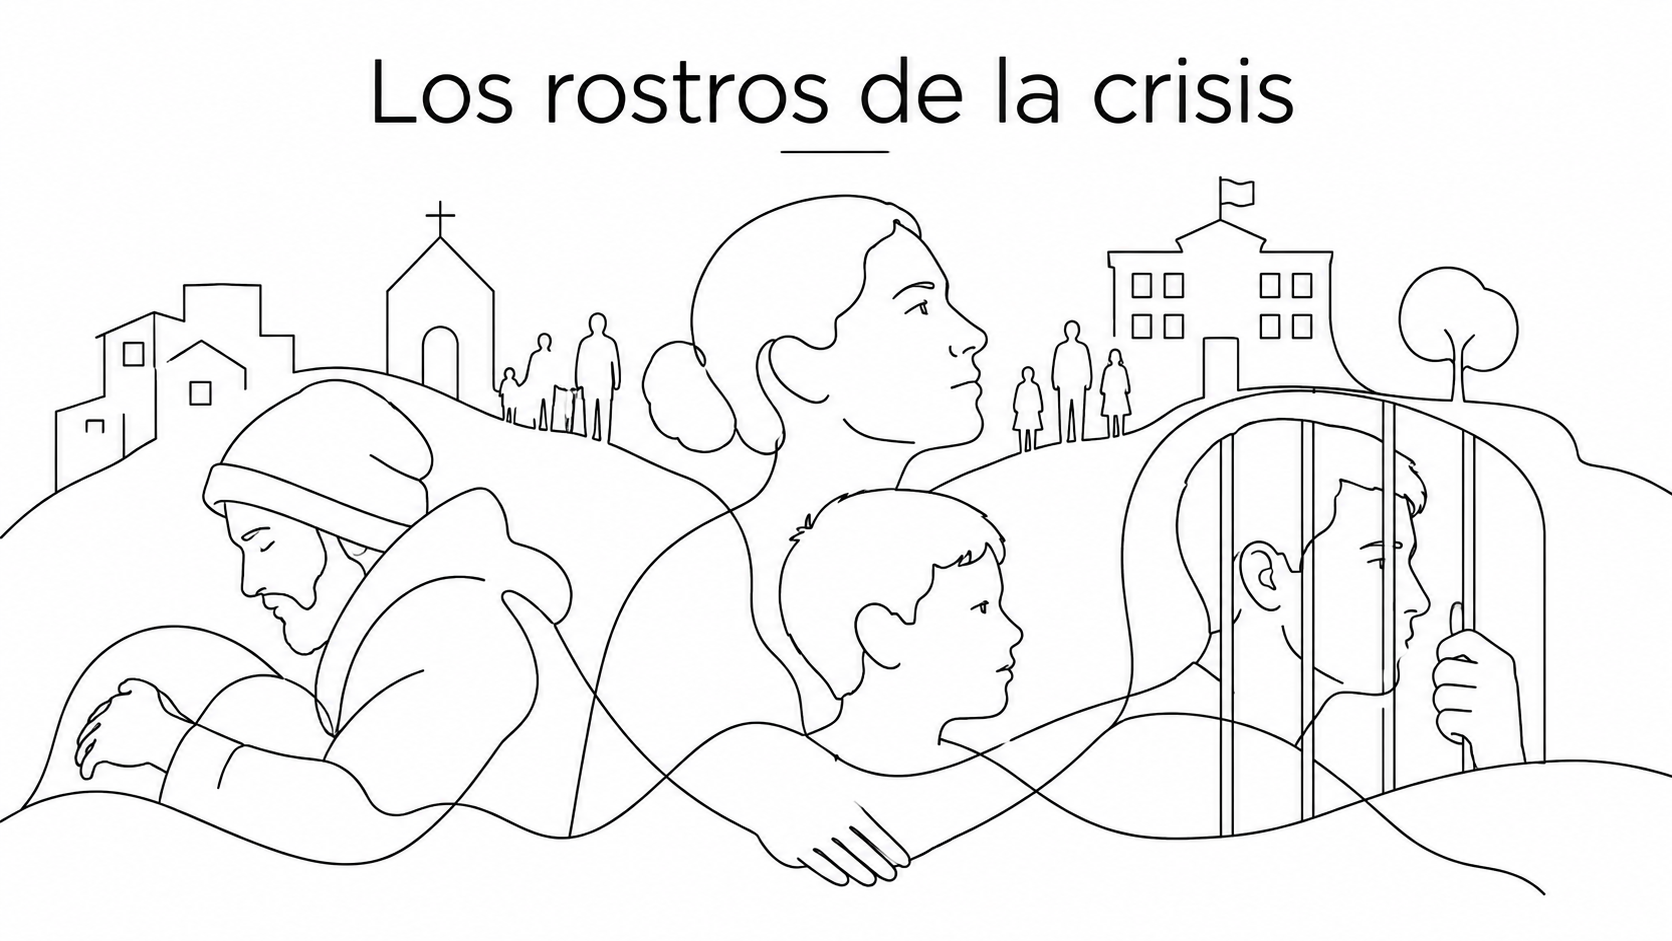
\includegraphics[scale=0.2]{rostrosdelacrisis.png}
		\caption{Los rostros de la crisis}
	\end{figure}
	
	
	\section{Nuestros barrios}
	
	Nuestros territorios están marcados hoy por un tejido social deshilachado, donde la pérdida de raíces y un individualismo extremo erosionan la noción de pueblo. En estas comunidades, la problemática de las sustancias no es un hecho aislado, sino un entramado que afecta todos los elementos vitales de la convivencia. Se observa que el narcotráfico se ha constituido en el organizador de la vida cotidiana ante el repliegue o la ausencia de las instituciones estatales, ocupando un lugar de poder que le permite regular desde la seguridad hasta la economía doméstica de las familias.
	
	Esta narcocultura funciona como una estructura que impone fronteras invisibles en el barrio, donde el simple movimiento de un sector a otro puede representar un riesgo para la vida. En las barriadas más postergadas, el crimen organizado ofrece el único camino de ascenso social visible, transformando la ética del trabajo por la lógica del dinero fácil. La realidad es cruda: los búnkeres se han convertido en los nuevos centros de referencia comercial del barrio y la venta de sustancias se ha atomizado de tal modo que los propios usuarios se ven empujados a la comercialización para sostener su consumo.
	
	\marginnote{\textit{Christus Vivit} N° 71-74\label{FCV}}
	
	El aspecto más crítico de este diagnóstico es la captación planificada de la infancia. Niños y adolescentes son utilizados como eslabones de la cadena delictiva bajo la figura de soldaditos o microtraficantes. Las crónicas territoriales coinciden en reportar casos de inicio del consumo en barrios populares desde los 8 o 9 años de edad, una realidad que contrasta con las estadísticas nacionales —que suelen situar el promedio de inicio entre los 13 y 15 años— y que evidencia la particular desprotección de las infancias en los sectores de mayor exclusión. A esto se suma una marcada feminización de la pobreza, donde las mujeres enfrentan solas la crianza en entornos de violencia, quedando frecuentemente atrapadas entre la necesidad de subsistencia y la desprotección absoluta.
	
	Se detecta, asimismo, una fragmentación de la respuesta institucional. El Estado suele llegar de forma tardía o mediante procesos burocráticos que resultan ajenos a la historia y los vínculos de las personas. El barrio se ha convertido en un escenario de disputa por la subjetividad, donde el mensaje del consumo inmediato compite con la posibilidad de una vida digna. Actualmente, la realidad de las esquinas y los pasillos muestra que el enfoque meramente asistencial resulta insuficiente frente a la ruptura profunda de los lazos sociales y la desolación de comunidades enteras que ven al territorio como un lugar de descarte.
	
	\section{Nuestras parroquias}
	
	Al observar la realidad de nuestras comunidades eclesiales, se detecta una tensión persistente entre el mandato del Evangelio y la práctica operativa frente al consumo. Muchas parroquias funcionan bajo una lógica predominantemente administrativa o de sacristía, replegadas en el mantenimiento de un orden interno y guardando una distancia prudente del dolor que habita en sus territorios. Esta actitud ignora frecuentemente que la problemática de las adicciones ya ha penetrado la vida de los propios fieles, tratándola como una realidad ajena que no requiere una respuesta pastoral específica.
	
	Existe una tendencia recurrente a dialectizar la realidad, clasificando a las personas entre los de adentro y los de afuera, o entre integrados y excluidos. Esta mirada suele etiquetar al usuario de sustancias bajo categorías morales de pecado o delincuencia, lo que oscurece su dignidad ontológica. Se observa que la rigidez en los horarios y los procedimientos institucionales suele anteponerse al caos existencial que introduce quien llega en situación de crisis. Esta dinámica genera un ambiente que es percibido como expulsivo por aquellos que están rotos, quienes encuentran en la estructura parroquial más una aduana de control que una casa de acogida.
	
	El diagnóstico revela, además, que la respuesta eclesial suele ser tardía. Se reconoce que la llegada de un joven a la cárcel o a un instituto de menores es, en muchos casos, el resultado de una comunidad que no logró ofrecer una red de contención previa. Esta demora se profundiza por una falta de comprensión del problema en los agentes pastorales, quienes a menudo consideran que la Iglesia no posee herramientas para este campo y delegan la responsabilidad exclusivamente en especialistas, trabajadores sociales o en el Estado. Esta desvinculación no solo mutila la dimensión social del mensaje cristiano, sino que deja en la orfandad a las familias que acuden a los templos buscando un consuelo y un acompañamiento que no encuentran en la burocracia estatal.
	
	\section{Nuestras escuelas}
	
	El ámbito educativo en la región atraviesa una crisis de sentido que se manifiesta en una profunda desconexión entre la institución y la realidad vital de los jóvenes. En los territorios más vulnerables, los agentes reportan que en los contextos de mayor vulnerabilidad hasta el 50 por ciento de los adolescentes abandonan la escuela secundaria debido a que el sistema no logra responder a sus necesidades ni ofrecer un horizonte atractivo. La escuela, que debería funcionar como un agente de socialización primario, es percibida a menudo como un espacio ajeno donde los contenidos académicos no logran entrar en diálogo con las urgencias del barrio.
	
	Se detecta con alarma que el consumo de sustancias ha permeado los muros escolares a edades cada vez más tempranas, reportándose casos de consumo problemático incluso en los primeros años de la educación primaria. Frente a esta realidad, la respuesta institucional suele oscilar entre la indiferencia y una sobreintervención fragmentada. En este último escenario, diversos actores como centros de salud, juzgados y organismos sociales actúan sobre un mismo niño sin coordinación alguna, lo que deriva en un descuartizamiento de su situación personal. Esta dinámica no solo resulta ineficaz, sino que vulnera la intimidad de los estudiantes al hacer circular información sensible por todo el entorno comunitario sin criterios de cuidado integral.
	
	El diagnóstico revela también una notoria falta de preparación en los cuerpos docentes y directivos para acompañar la complejidad de las adicciones. Ante la carencia de herramientas de detección y abordaje, se recurre frecuentemente a etiquetas estigmatizantes que terminan por expulsar al joven del sistema educativo, reforzando su exclusión. Asimismo, se observa una incoherencia institucional en ciertas comunidades donde, mientras se intenta prevenir el consumo, se naturaliza la presencia y venta de alcohol en eventos escolares para recaudar fondos, enviando mensajes contradictorios a los menores.
	
	Finalmente, el aula se ve impactada por un entorno macro desorganizado donde la pobreza, la desnutrición y la ausencia de referentes adultos transforman el espacio escolar en un simple lugar de paso. La educación ha quedado reducida en muchos casos a la mera transmisión de datos, perdiendo su capacidad de escucha y de formación de ciudadanos con propósito. En el estado actual de las cosas, la escuela se muestra debilitada en su función de contención, perdiendo la batalla por la subjetividad de los jóvenes frente a la oferta inmediata y evasiva de las sustancias.
	
	\section{La situación particular de las mujeres}
	
	La experiencia de las mujeres atravesadas por el consumo en la región revela una trama de vulnerabilidad específica que difiere profundamente de la masculina. Se observa una doble condena, social y moral: la mujer es juzgada no solo por el uso de sustancias, sino por el incumplimiento del rol cultural de madre y cuidadora del hogar. Este estigma genera una internalización del rechazo, donde la persona llega a percibir su situación como una vergüenza personal, lo que alimenta ciclos de culpa y autodesprecio que suelen paralizar la búsqueda de acompañamiento.
	
	En el ámbito vincular, se detecta un marcado contraste respecto a los varones. Mientras ellos suelen contar con una red de contención femenina —madres, esposas o hermanas— durante sus procesos, las mujeres enfrentan frecuentemente el abandono de sus parejas y familias al hacerse visible el consumo. A esta soledad estructural se suma el temor constante a la intervención estatal; muchas madres ocultan su problemática ante el miedo a que los organismos de protección les arrebaten la custodia de sus hijos, percibiendo al sistema más como una instancia punitiva que restauradora.
	
	Desde la dimensión biológica, se identifica el fenómeno denominado efecto telescopio, por el cual las mujeres transitan desde el primer uso hacia la dependencia severa y el daño físico en un tiempo mucho más acelerado que los varones. Factores fisiológicos, como la mayor proporción de tejido adiposo donde permanecen impregnadas las sustancias psicoactivas, dificultan y prolongan los procesos de desintoxicación, incrementando el riesgo de cirrosis, patologías duales y un deterioro orgánico precoz.
	
	El diagnóstico territorial señala que el consumo femenino funciona, en gran medida, como un intento autoterapéutico frente a traumas complejos. Historias de violencia de género, abusos en la infancia, negligencia y orfandad configuran una fractura interna que la sustancia busca anestesiar. En contextos de feminización de la pobreza, la falta de acceso a tierra, techo y trabajo digno empuja a muchas mujeres a estrategias de supervivencia de alto riesgo, como el narcomenudeo o la prostitución, para sostener la economía familiar, lo que las expone a nuevos círculos de violencia y consumo.
	
	Finalmente, se advierten serias deficiencias en el sistema de salud pública. Existe una carencia crítica de centros de atención específicos para mujeres y persiste un fuerte estigma en centros hospitalarios generales, donde se registran situaciones de maltrato, humillación o segregación hacia mujeres embarazadas o con VIH. La respuesta institucional suele ignorar la necesidad de un abordaje integral que considere la maternidad y la reparación de los vínculos primarios como ejes centrales del proceso diagnóstico.
	
	\section{Las familias y los más chicos}
	
	Al observar la realidad de los más pequeños en los territorios, se identifica una de las heridas más profundas de la región: el descenso drástico de la edad de inicio del consumo, donde los agentes pastorales reportan casos en sectores populares desde los 8 o 9 años. Este fenómeno se manifiesta como el resultado de una orfandad funcional, donde niños y adolescentes crecen en entornos en los que los adultos referentes han dejado de ser figuras protectoras para volverse ausentes o invisibles. Se detecta que las familias, que deberían constituir un puerto seguro, se encuentran frecuentemente fragmentadas o atravesadas por la misma problemática del consumo, la pobreza estructural y el hacinamiento. Esta desolación empuja a los menores a la calle no solo en busca de la sustancia, sino como un modo de escapar de dolores intolerables o de encontrar el afecto y la pertenencia que no hallan en sus hogares.
	
	Las comunidades infantiles en estos contextos están marcadas por el trauma complejo. El maltrato intrafamiliar, la negligencia y el abuso sexual configuran un escenario que condiciona el desarrollo desde la temprana infancia. En este marco, el narcotráfico opera como un sistema de captación planificada, reclutando a niños de entre 12 y 16 años para utilizarlos como soldaditos o microtraficantes. Esta estructura delictiva se presenta como el único camino de ascenso social visible ante el repliegue de las instituciones estatales, aprovechándose de la vulnerabilidad biológica de un cerebro en desarrollo cuya corteza prefrontal\index{corteza prefrontal} inmadura carece de los frenos necesarios para evaluar el riesgo o resistir la presión del grupo.
	
	En muchos casos, quienes debieran ser figuras protectoras no asumen plenamente el rol de padre o madre. Presentan dificultades para establecer límites y para adaptarse a las exigencias que implican la vida familiar y la llegada de los hijos, sin haber desarrollado las habilidades necesarias para ejercer una crianza adecuada. Generalmente, estos adultos tampoco estuvieron preparados para formar una familia: provienen de experiencias similares y no logran romper el círculo que termina repitiéndose en su propia vivencia como padres.
	
	El diagnóstico revela así una repetición generacional de estas historias, donde muchos de los adultos que hoy atraviesan el consumo son los niños heridos del pasado que nunca contaron con una red de contención efectiva. A esta situación se suma el impacto de la desnutrición y la malnutrición que, combinadas con el uso de sustancias altamente tóxicas como el crack o la pasta base, generan niveles de deterioro cognitivo y discapacidad que comprometen el futuro de miles de menores en situación de exclusión. La feminización de la pobreza también juega un rol central: las madres enfrentan en soledad la crianza y el estigma social, lo que deriva en un miedo constante a ser sancionadas por el sistema de protección estatal.
	
	Finalmente, se reconoce la emergencia de nuevas formas de aislamiento dentro del hogar a través del entorno digital. Estudios internacionales y la observación territorial coinciden en que los niños pueden pasar más de ocho horas diarias frente a pantallas, exponiéndose a una sobrecarga de información y, de manera creciente, a la ludopatía por apuestas en línea. Este entorno genera una desconexión progresiva de las emociones y de los vínculos familiares primarios. La liberación constante de dopamina provocada por los dispositivos electrónicos altera los circuitos cerebrales de placer de forma análoga a la de las sustancias químicas, profundizando la ansiedad y el aislamiento en el seno mismo del hogar.
	
	\section{Las nuevas tecnologías}
	
	Al observar la realidad de nuestras comunidades, se reconoce la emergencia de un nuevo escenario de riesgo: el territorio digital. Este espacio, aunque carece de geografía física, es donde hoy se juega gran parte de la existencia, la identidad y los vínculos de los jóvenes. No se trata solo de herramientas de comunicación, sino de un entorno que moldea la subjetividad a través de mecanismos de impulsividad y compulsividad que alteran los centros de placer de forma análoga a las sustancias químicas.
	
	Se detecta una alarmante colonización del tiempo y la atención, donde los adolescentes pasan varias horas diarias frente a las pantallas, con estimaciones internacionales que superan las ocho horas en algunos contextos. Este consumo genera un estado de alerta constante debido al flujo incesante de notificaciones —que pueden alcanzar los centenares diarios—, lo que alimenta el fenómeno conocido como FOMO (miedo a quedar fuera). Esta sobrecarga de información deriva en una ansiedad persistente por la aprobación de los pares y una fragmentación de la atención que dificulta el desarrollo de procesos reflexivos profundos.
	
	Se observa con especial preocupación la mutación del entretenimiento hacia la ludopatía por apuestas online, particularmente en menores de edad. Este camino suele iniciarse de forma insidiosa a través de videojuegos aparentemente gratuitos que introducen lógicas de mercado y competencia, evolucionando luego hacia las apuestas por internet. Esta forma de adicción conductual funciona como una vía de escape para anestesiar malestares emocionales o incertidumbres de la vida diaria, generando un dolor secundario marcado por la culpa y el aislamiento absoluto dentro de la propia habitación.
	
	El impacto de estas tecnologías se manifiesta también en la salud física y en el tejido familiar. Se reportan problemas de columna y perturbaciones graves del sueño vinculadas a posturas y horarios inadecuados que alteran el ritmo vital. En el hogar, la dependencia del dispositivo genera una desconexión de las emociones y de los vínculos primarios, sustituyendo el diálogo por un entretenimiento constante que invisibiliza los problemas ante los padres hasta que el deterioro es severo. El diagnóstico resalta que este sistema está diseñado para vencer el autocontrol de los jóvenes, cuya corteza prefrontal —el freno biológico de los impulsos— se encuentra todavía en pleno proceso de desarrollo.
	
	
	
	\section{La salud}
	
	Al observar la salud física de las personas atravesadas por el consumo, se reconoce una realidad de fragilidad extrema y abandono sistémico. El diagnóstico territorial revela una situación de orfandad asistencial, donde el sistema de salud formal suele encontrar un tope o límite ante la marginalidad. Se detecta que las instituciones sanitarias presuponen que el paciente posee condiciones basales de vida, como techo, comida o estabilidad habitacional, cuya ausencia anula la eficacia de cualquier tratamiento médico y expulsa a los sujetos del circuito de cuidado.
	
	Las barreras de acceso se manifiestan a través de una burocracia que resulta expulsiva para los más pobres. El sistema exige con frecuencia documentos de identidad, cumplimiento de horarios rígidos y traslados costosos que las personas en situación de calle o de barrios periféricos no pueden sostener. En zonas rurales o de montaña, esta situación se agrava por la lejanía geográfica y la falta de planificación, lo que interrumpe la continuidad de procesos vitales. Se observa que el sistema está fragmentado y saturado, ofreciendo respuestas administrativas que priorizan el procedimiento por sobre la urgencia del sufriente.
	
	Un elemento crítico del diagnóstico es el estigma y el trato discriminatorio dentro de los centros médicos. Los testimonios de los agentes coinciden en que el personal sanitario a menudo maltrata, segrega o ignora a las personas en situación de consumo o personas con VIH. Se han registrado situaciones donde madres embarazadas en situación de consumo son segregadas en las salas de espera de los hospitales generales, un gesto de rechazo que las aleja de la posibilidad de pedir ayuda. Este estigma funciona como una barrera invisible que profundiza la desprotección y desalienta el acercamiento de las poblaciones más vulnerables a la salud pública.
	
	El deterioro físico derivado del consumo crónico, especialmente de sustancias altamente tóxicas como el crack o la pasta base, genera daños neurológicos y cognitivos severos, comprometiendo gravemente el sistema inmunológico. Esta vulnerabilidad biológica facilita la propagación de enfermedades marcadoras de la pobreza, como la tuberculosis, el VIH/SIDA y las hepatitis. El diagnóstico suele ser tardío debido a la falta de una red de cuidados preventivos, lo que deriva en que muchas personas lleguen a los hospitales en etapas terminales. El resultado es un índice alarmante de muertes que se describen como vergonzosas y absolutamente prevenibles.
	
	Finalmente, se identifica una problemática específica en la salud 
	neonatal y la infancia. Se advierte un incremento de bebés que nacen 
	con síndrome de abstinencia neonatal, epilepsias o discapacidades 
	vinculadas al consumo materno durante la gestación. En las mujeres, 
	el ya mencionado efecto telescopio acelera el daño orgánico, 
	resultando en patologías graves en tiempos mucho más breves que en 
	los varones. Esta realidad evidencia que la crisis de salud en los 
	territorios no es solo un problema de falta de medicinas, sino de 
	una estructura institucional que no logra reconocer la dignidad de 
	quienes habitan las periferias.
	
	\section{Salud mental}
	
	Al observar la realidad de nuestros territorios, se reconoce que la salud mental es un componente crítico y frecuentemente invisibilizado en el drama de las adicciones. El diagnóstico revela que, según estimaciones consistentes en la literatura clínica internacional, aproximadamente el 50 por ciento de las personas que padecen un trastorno por uso de sustancias presentan también un trastorno mental coocurrente\index{patología dual}, lo que configura la complejidad de la patología dual. Se detecta que el consumo no es el problema en sí mismo, sino el síntoma de una fractura interna o un intento autoterapéutico de anestesiar una vida que se ha vuelto intolerable debido a heridas profundas.
	
	La problemática se fundamenta en una desregulación del sistema nervioso central ante estímulos que el sujeto no puede significar adecuadamente. El consumo aparece entonces como una herramienta de fuga o desconexión frente a un mundo percibido como amenazante, especialmente cuando existen redes de memoria desadaptativas que almacenan traumas, abusos o abandono en la infancia. Se identifica una prevalencia significativa de diversas organizaciones de la personalidad en los barrios, destacándose las estructuras limítrofes o borderline, así como cuadros psicóticos marcados por una gran fragilidad y pérdida del juicio de realidad.
	
	Se observa con preocupación que el sistema de salud formal suele encontrar un tope ante esta marginalidad. Las instituciones ofrecen a menudo respuestas fragmentadas que ignoran la necesidad de abordar la integridad de la persona, tratando la adicción y el trastorno mental como compartimentos estancos que no se comunican entre sí. Esta falta de mirada integral deriva en que los cuadros psiquiátricos de base y los traumas previos queden desatendidos, lo que suele conducir a recaídas recurrentes que el propio sistema penaliza o malinterpreta como falta de voluntad.
	
	Finalmente, el diagnóstico resalta el peso del estigma y la vergüenza. El paciente suele internalizar el rechazo social, transformándolo en un sentimiento de indignidad que sabotea sus propios intentos de bienestar. La realidad de nuestros hermanos revela que la adicción es la manifestación visible de una orfandad emocional profunda, donde el vacío existencial y la falta de puntos de referencia claros dejan al individuo sin herramientas psíquicas para enfrentar el dolor de su propia historia.
	
	\section{El drama del trabajo}
	
	Al recibir la realidad de nuestros territorios, reconocemos que el trabajo no es solo un medio de subsistencia, sino el eje vertebrador que otorga dignidad y sentido a la vida cotidiana. Sin embargo, hoy nos duele constatar que este eje se encuentra frecuentemente fracturado, convirtiéndose en un escenario de profundo sufrimiento para nuestros pueblos. El drama del trabajo se manifiesta tanto en la angustia del desempleo como en la deshumanización de las condiciones laborales, realidades que deben abordarse como heridas profundas en la salud integral de la persona.
	
	La falta de empleo no debe mirarse solo desde las estadísticas económicas; es una verdadera urgencia que desestructura el corazón y la mente. La ausencia de una tarea que ordene el día genera bloques de \textit{tiempo vacío} que aumentan la vulnerabilidad ante el consumo, donde la droga aparece como una falsa anestesia para mitigar el dolor del desamparo. Esta situación empuja al hermano hacia una \textit{deriva social} que suele culminar en la ruptura de los lazos familiares y, en los casos más extremos, en la situación de calle. Para esta pastoral, el desempleo es un factor predictor de recaída que requiere una respuesta de misericordia y justicia inmediata.
	
	El mundo del trabajo no siempre es un espacio de realización; a menudo presenta condiciones que enferman y predisponen al consumo. Observamos con dolor cómo las labores en climas extremos o ritmos extenuantes inducen al uso de sustancias para \textit{aguantar} la fatiga. La precariedad laboral actúa como una pandemia tóxica que penetra en la subjetividad de los trabajadores, produciendo ansiedad y una profunda soledad. En muchos sectores, se vive una \textit{privatización del agotamiento}, donde el malestar sistémico es cargado como un fracaso personal, ocultando las estructuras de pecado que deshumanizan la labor diaria.
	
	En el otro extremo del desempleo, nos encontramos con el fenómeno del \textit{workaholism} o adicción al trabajo. Es una patología que la sociedad suele alabar bajo la máscara del éxito y la eficiencia, pero que esconde una necesidad incontrolable de llenar vacíos existenciales. La persona dependiente del trabajo basa su valor únicamente en la productividad, descuidando su salud y sus vínculos sagrados. Es vital que el agente pastoral esté atento a los procesos de recuperación, ya que a menudo la compulsión por la sustancia es reemplazada por esta laborodependencia compulsiva. Esta \textit{situación encubierta} no es sino otra forma de dependencia que conduce inevitablemente al agotamiento espiritual y a la pérdida del sentido de la vida en comunidad.
	
	
	\section{Nuestros hermanos en la calle}
	
	Al observar la realidad de quienes habitan las calles de nuestra región, se reconoce una de las expresiones más crudas de la cultura del descarte\index{cultura del descarte}. Esta situación no se limita a una carencia de recursos económicos, sino que responde a una trayectoria de vulnerabilidad múltiple marcada por rupturas profundas en los vínculos familiares, abandonos tempranos y duelos que no han sido gestionados. Se detecta que muchos hermanos perciben la calle, de manera paradójica, como un espacio de falsa libertad; ante la ausencia de normas y redes de apoyo, esta autonomía aparente los mantiene alejados de los organismos gubernamentales y perpetúa ciclos de marginalización extrema.
	
	En este contexto, el uso de sustancias psicoactivas funciona como un intento autoterapéutico para anestesiar una realidad que se ha vuelto intolerable. La sustancia es utilizada como una herramienta para procesar el impacto del frío, el hambre y la soledad, así como la desregulación emocional provocada por heridas de infancia, abusos y maltratos. El consumo actúa, por tanto, como un mecanismo de fuga y desconexión frente a un entorno que el individuo percibe como hostil y amenazante.
	
	El diagnóstico revela que el sistema de salud formal suele encontrar un tope o límite ante la marginalidad de la calle. Las instituciones sanitarias y sociales presuponen frecuentemente que el paciente tiene resueltas sus necesidades básicas, exigiendo para el acceso a tratamientos condiciones de estabilidad habitacional, alimentación y documentación que la persona no posee. Esta rigidez burocrática resulta expulsiva y deriva en una alta tasa de muertes absolutamente prevenibles por enfermedades infecciosas como la tuberculosis, el VIH y la hepatitis C, ya que el sistema no logra flexibilizar sus protocolos para asegurar la adherencia a los tratamientos en condiciones de intemperie.
	
	Se observa, asimismo, que ante la orfandad funcional de sus hogares de origen, las personas en situación de calle tejen lazos de apoyo mutuo en el propio territorio de la calle, conformando una red vincular que opera como una familia alternativa. Estos vínculos son tan significativos que a menudo se convierten en un factor de añoranza que dificulta los procesos de recuperación si no se ofrece una comunidad de pertenencia similar. Finalmente, el diagnóstico destaca que el estigma social los vuelve invisibles ante la ciudadanía, privándolos no solo del acceso a derechos básicos como la vivienda, sino del reconocimiento fundamental de ser llamados por su propio nombre.
	
	\section{La población travesti-trans}
	
	Al observar la realidad de la población travesti-trans en la región, se identifica que la identidad, la exclusión y el consumo forman parte de una misma trama de vulnerabilidad múltiple. Las trayectorias de estas personas suelen estar marcadas por una expulsión temprana de los espacios que debieron brindarles cuidado, tales como la familia, la escuela, el ámbito laboral y el sistema de salud. Esta exclusión sostenida deja huellas profundas en la interioridad, donde el consumo de sustancias aparece como un recurso para intentar aliviar el dolor, la soledad y la falta de pertenencia generada por el rechazo sistémico del entorno social.
	
	Para gran parte de esta población, el sistema ha funcionado bajo un binomio restrictivo que limita sus posibilidades de subsistencia casi exclusivamente al trabajo sexual o a rubros informales como la peluquería, sin ofrecer alternativas reales de formación o empleo. En este escenario, la prostitución se vincula estrechamente con el consumo, ya que la sustancia se convierte en una herramienta de sobrevivencia necesaria para soportar las condiciones de la calle, el frío, el hambre, el miedo y la violencia. Se detecta, además, que la vulnerabilidad es frecuentemente explotada por terceros que fomentan el uso de drogas para facilitar situaciones de abuso o para asegurar el control sobre las personas.
	
	El diagnóstico revela también un conflicto particular vinculado a los procesos de transición de identidad. Se observa que la brecha entre la imagen mental deseada y la realidad física puede generar dolores simbólicos y una ansiedad profunda que detonan el uso de sustancias como una vía de escape. Asimismo, esta población enfrenta una fragmentación extrema en el acceso a la salud, donde persiste un estigma que las hace sentir ajenas o señaladas incluso en ámbitos institucionales y comunitarios. El consumo actúa, en última instancia, como una sutura fallida para anestesiar heridas de maltrato e injusticia acumuladas a lo largo de la vida.
	
	Desde la dimensión espiritual, se percibe una situación de orfandad institucional. Ante el rechazo o la invisibilidad en las estructuras religiosas tradicionales, muchas personas han buscado refugio en creencias alternativas para encontrar la protección que la sociedad les niega. Detrás de la coraza de dureza que han construido para sobrevivir a la hostilidad del entorno, se detecta una esencia fragilizada y cansada que evidencia la falta de una red de apoyo que reconozca su dignidad fundamental. El estado actual de las cosas muestra que el sistema limita drásticamente su esperanza de vida y su capacidad de proyectar un futuro fuera de los márgenes de la exclusión.
	
	\textbf{Una precisión pastoral es necesaria.} Este manual aborda la realidad de la población travesti-trans\index{acompañamiento!de población travesti-trans} desde la perspectiva específica de su competencia: el acompañamiento y la prevención de las adicciones en contextos de exclusión. La inclusión de esta población en el diagnóstico no presupone ni implica una toma de posición doctrinal sobre las teorías contemporáneas de la identidad de género, cuyo discernimiento corresponde a otros ámbitos del magisterio eclesial. Lo que sí presupone es una opción inequívoca por la dignidad y la vida de toda persona humana, independientemente de su condición, su identidad o su historia. El Papa Francisco ha sido claro al respecto: la pastoral no puede quedar subordinada a un debate teórico cuando hay personas que mueren en la calle sin que nadie les pregunte su nombre. La tarea de este manual es precisamente esa: preguntarles el nombre, reconocer su dignidad ontológica como hijos de Dios y ofrecer el acompañamiento que ninguna otra institución les está brindando. Que la Iglesia acompañe a estas personas no requiere haber agotado todas las cuestiones doctrinales que su realidad plantea; requiere haber entendido que nadie puede quedar fuera del cuidado pastoral mientras viva en el sufrimiento. Como enseña el Retablo de Isenheim, los antonianos no pedían diagnóstico antes de abrir la puerta del monasterio.
	
	\section{Las cárceles}
	
	Al observar la realidad del mundo penitenciario en la región, se identifica una extensión directa de la vulnerabilidad que ya habita en los barrios populares. Las cárceles están pobladas mayoritariamente por personas en situación de pobreza, lo que revela un sistema donde el consumo problemático y el delito cometido para sostenerlo atrapan a los sectores más excluidos en un ciclo de reincidencia. Se detecta que el encierro, lejos de funcionar como un espacio de resocialización, suele profundizar la problemática de las adicciones.
	
	La dinámica interna de los penales se caracteriza por la existencia de un mercado de sustancias donde la droga funciona como moneda de cambio y herramienta de poder. Se observa que el consumo dentro del encierro es caótico y está frecuentemente ligado a situaciones de violencia. Existen estructuras internas que esclavizan a los internos a través de la deuda; se reportan casos donde, ante la negativa de un interno a consumir o vender, se ejerce violencia física contra él para obligar a su familia a enviar dinero desde el exterior. Esta realidad convierte al penal en un escenario de mayor riesgo y desprotección que la propia calle.
	
	En el ámbito de las cárceles de menores, el diagnóstico es aún más crítico. Se registra que la gran mayoría de los adolescentes privados de su libertad lo están por causas vinculadas directamente al uso de sustancias. El impacto del consumo en el penal genera daños irreversibles en el desarrollo neurológico, considerando que el cerebro humano completa su maduración hacia los 25 años. Asimismo, se detecta una barrera en el acceso a la salud mental: muchos internos que padecen patologías psiquiátricas rechazan la medicación necesaria por temor a que el sistema judicial utilice ese diagnóstico para alargar sus penas o denegarles salidas transitorias bajo la etiqueta de enfermos mentales.
	
	El diagnóstico incluye también la situación del personal penitenciario, quienes a menudo trabajan en condiciones de precariedad similares a las de los internos. Se observa que muchos agentes están atravesados por la misma problemática del consumo, una realidad que permanece silenciada por el estigma institucional. Esta situación impide que el personal actúe como un referente de cuidado y los sitúa, en ocasiones, como parte del engranaje del mercado interno de sustancias.
	
	Finalmente, se identifica el fenómeno denominado el abismo de la libertad. La etapa más compleja del proceso no se registra durante el encierro, sino al momento del egreso. Existe un vacío absoluto en el acompañamiento post-penitenciario\index{acompañamiento!post-penitenciario}, donde el Estado suele dar por terminada su intervención al firmar el acta de libertad. El liberado sale al portón del penal sin recursos económicos, sin empleo y, frecuentemente, sin una red familiar que lo reciba. Este desamparo estructural empuja al individuo a regresar al mismo entorno de consumo y supervivencia delictiva que lo llevó inicialmente a la cárcel, evidenciando la falta de casas de medio camino o redes de contención que sostengan la transición hacia la vida en comunidad.
	
	\section{El narcotráfico y la globalización del crimen organizado}
	
	Al observar la realidad de nuestra región, se reconoce que el narcotráfico no es un fenómeno delictivo aislado ni puramente local, sino una red global con una sofisticada ingeniería económica y una logística de distribución capilarizada en todo el continente. Este sistema opera como una estructura transnacional donde las sustancias producidas en países como Colombia o Perú transitan por rutas controladas en Paraguay y utilizan nodos estratégicos, como los puertos fluviales de la hidrovía, para su salida hacia los mercados internacionales. Se estima que el mercado global de drogas ilícitas representa cerca del 1 por ciento del Producto Interno Bruto mundial según las Naciones Unidas, cifra que se amplía significativamente al considerar el entramado completo del crimen organizado —que incluye el lavado de activos, la trata de personas, el tráfico de armas y la corrupción institucional—, logrando infiltrarse en la economía legal a través de la complicidad de instituciones bancarias, desarrollos hoteleros, cadenas de supermercados y estudios jurídicos que facilitan el blanqueo de capital ilícito.
	
	En las barriadas más postergadas, donde el Estado se ha replegado o su presencia es puramente formal, el narcotráfico ha ocupado ese vacío constituyéndose en el nuevo organizador de la vida cotidiana. Su poder no se limita a la comercialización de sustancias, sino que funciona como un ente regulador que presta dinero a los vecinos ante la falta de crédito formal, provee transporte privado para urgencias médicas nocturnas y genera una fuente de empleo informal y precario para cientos de personas en un solo territorio. Esta presencia territorial impone leyes propias y fronteras invisibles que delimitan la libre circulación de los vecinos; se observa que salir de un sector controlado por una banda para acudir a una institución de salud en otro sector puede representar un riesgo de muerte. El narco dicta las normas de convivencia, desplazando la autoridad legítima por una dictadura moderna que secuestra la paz de las comunidades.
	
	En esta disputa por el territorio y la subjetividad de nuestros pueblos, la \textit{narcocultura} se erige como el reverso tenebroso de una verdadera \textit{ética del cuidado}\index{ética del cuidado}. Mientras la primera impone un relato de muerte y ostentación, basando el ascenso social en la violencia y el dinero fácil, la ética del cuidado —encarnada en nuestra pastoral— propone una \textit{pedagogía de la ternura}\index{pedagogía de la ternura} que protege la vida sagrada y reconstruye los vínculos rotos frente a la lógica del descarte.
	
	La narcocultura ofrece a los jóvenes una pertenencia falsa y una identidad basada en el poder de las armas; frente a esto, el cuidado comunitario construye \textit{mesas compartidas} donde la orfandad se cura con la presencia significativa\index{presencia significativa} y el vínculo. Mientras el narco traza fronteras invisibles que dividen y matan, el cuidado teje redes de projimidad\index{projimidad|textbf} (hacerse presente en la vida del otro, compartir su realidad, escucharlo y acompañarlo desde dentro de su situación concreta) que integran al hermano, devolviéndole su dignidad ontológica de hijo de Dios.
	
	
	Este sistema se sostiene sobre formas extremas de crueldad y esclavitud moderna. El diagnóstico territorial revela una captación planificada de la infancia, donde niños y adolescentes de entre 12 y 16 años son reclutados como eslabones de vigilancia o microtraficantes bajo la promesa de un ascenso social que es, en realidad, un sistema de descarte. En zonas rurales, se detecta el uso de niños para tareas de procesamiento de cultivos con el consentimiento de familias sumidas en la pobreza extrema. Asimismo, se advierte una vulneración profunda de la mujer: en contextos de desprotección absoluta, niñas y adolescentes son utilizadas por redes de trata o vendidas a narcotraficantes como estrategia de supervivencia económica. La consolidación de estas estructuras ha disparado el fenómeno del sicariato, donde la vida humana pierde su valor intrínseco y se convierte en moneda de cambio.
	
	Se identifica que el avance del crimen organizado representa un riesgo directo para la estabilidad de las instituciones. La denominada narcopolítica ha generado estructuras paralelas donde jueces, policías y fiscales son captados por el poder financiero del tráfico, garantizando la impunidad y dejando desprotegida a la ciudadanía. Esta corrupción sistémica se apoya en una narcocultura que impone un relato de muerte y ostentación, transformando los valores tradicionales de la comunidad por una ética de la violencia y el consumo inmediato. El miedo generado por esta violencia estructural provoca el repliegue de las instituciones civiles, dejando el espacio público a merced de los mercaderes de la muerte.
	
	Finalmente, el diagnóstico resalta que el narcotráfico lucra con la fractura interna de los sujetos y la desolación de los territorios. Se observa que la adicción es el combustible que alimenta este negocio perverso, el cual aprovecha la falta de horizontes, educación y trabajo digno para convertir a los jóvenes en carne de cañón. El escenario actual muestra un mal organizado que utiliza la marginalidad para expandirse, creando un entramado de pecado social que erosiona la democracia y anula la posibilidad de un proyecto de vida digno para las mayorías excluidas.
	
	\section{Los Estados y las políticas públicas}
	
	Al observar la relación entre las estructuras estatales y la realidad de los territorios, el diagnóstico revela una marcada apatía e indiferencia gubernamental. Mientras el crimen organizado se consolida mediante una ingeniería económica global, las respuestas del Estado suelen ser insuficientes, tardías o inexistentes. Se detecta que, ante este repliegue institucional, la tarea de acompañamiento queda delegada de hecho en la sociedad civil y las comunidades de fe, evidenciando que la burocracia estatal no logra habitar los espacios de mayor vulnerabilidad.
	
	Un elemento crítico identificado por los agentes es la implementación de políticas de carácter sanitizante. Estas acciones se centran en tratar de limpiar el espacio público bajo un enfoque punitivo y criminalizante, considerando a las personas en situación de consumo o de calle como estorbos urbanos que deben ser removidos o escondidos. Esta lógica prioriza una seguridad ciudadana mal entendida sobre la dignidad de los sujetos, agotando los recursos públicos en la guerra contra el narcotráfico mientras se desatiende por completo la atención a las víctimas y la reducción de la demanda.
	
	Se observa, asimismo, una profunda fragmentación administrativa. El Estado opera mediante casillas burocráticas estancas —salud, justicia, vivienda, desarrollo social— que no se comunican entre sí. Esta falta de coordinación genera un sistema expulsivo: para acceder a un tratamiento médico, se exigen requisitos que el sujeto no puede cumplir, como poseer un documento de identidad o una estabilidad habitacional que el propio Estado no garantiza. De este modo, el sistema formal encuentra un tope o límite ante la marginalidad, ya que presupone condiciones basales de vida que los sectores más postergados no poseen.
	
	El diagnóstico advierte sobre una situación de orfandad institucional. Las estadísticas indican una desproporción en el gasto público, donde los presupuestos para prevención son mínimos en comparación con otras áreas. Existe la constatación de que el Estado es capaz de otorgar subsidios o beneficios administrativos, pero carece de la flexibilidad necesaria para generar comunidad. La burocracia no puede construir los vínculos de confianza, pertenencia y afecto que el diagnóstico territorial señala como los únicos elementos capaces de restaurar el lazo social.
	
	Finalmente, se reconoce el impacto de la narcopolítica en el debilitamiento del Estado de derecho. La corrupción de sectores del poder judicial, policial y político permite que el narcotráfico actúe como un organizador social ante la retirada de las instituciones legítimas. En este escenario, las políticas públicas pierden su función de herramientas de justicia y se transforman en instrumentos que profundizan la exclusión y el descarte de quienes se encuentran en situación de mayor fragilidad.
	
	\chapter{El Magisterio Eclesial}
	
	En este apartado nos proponemos recuperar y sistematizar los planteamientos fundamentales de la Iglesia sobre el fenómeno de las adicciones, centrándonos en el pensamiento de san Juan Pablo II y del Papa Francisco. Ambos pontífices han abordado esta problemática con una profundidad excepcional, aportando elementos esenciales para comprender la realidad que hoy enfrentamos en nuestros territorios.
	
	El magisterio de Juan Pablo II, plasmado en una sistematización de más de ochenta intervenciones, sentó las bases antropológicas al definir la adicción como una patología del espíritu y una manifestación de lo que denominó la cultura de la muerte. Por su parte, el Papa Francisco ha hecho mención al tema en 186 apariciones públicas, incluyendo documentos, homilías y discursos. Su magisterio ha actualizado esta mirada al insertar el drama de las adicciones dentro de la cultura del descarte\index{cultura del descarte!y magisterio de Francisco} y al denunciar al narcotráfico como una estructura de pecado que genera nuevas formas de esclavitud.
	
	A diferencia de ellos, el magisterio de Benedicto XVI no abordó el tema de la droga de forma sistemática, y más bien orientó sus reflexiones principalmente hacia las raíces de la secularización y la crisis ética global. Por esta razón, el desarrollo de la doctrina social y pastoral sobre el problema de las sustancias descansa primordialmente en los ejes trazados por Juan Pablo II y Francisco, cuyas enseñanzas nos permiten profundizar en el diagnóstico de esta crisis que atraviesa a nuestros pueblos.
	
	
	\section{Itinerario de la conciencia eclesial y nuevos paradigmas pastorales}
	
	La respuesta de la Iglesia frente al fenómeno de las adicciones y el consumo de sustancias no ha sido un proceso estático, sino el resultado de una toma de conciencia progresiva en diálogo con los signos de los tiempos. Esta maduración histórica ha permitido transitar desde una mirada meramente condenatoria o asistencialista hacia un enfoque de atención amante y acompañamiento integral. A continuación, se describen los cuatro pilares que configuran este itinerario\index{acompañamiento!itinerario histórico} y los nuevos paradigmas que sustentan la acción pastoral actual. 
	
	
	
	\paragraph{1. Evolución histórica del Magisterio y la acción pastoral}
	
	El camino recorrido por la Iglesia en las últimas cinco décadas puede estructurarse en cinco hitos fundamentales que marcan la evolución de su mirada:
	
	\begin{itemize}
		\tightlist
		\item
		\textbf{La década de los 70 y la Evangelización de las periferias:} Bajo el impulso de la exhortación \emph{Evangelii Nuntiandi\label{PVIEN}} de Pablo VI, la Iglesia reconoció que su razón de ser más honda es llevar la Buena Noticia a todos los ambientes. Esto implicó la necesidad de que la evangelización llegara a las «periferias humanas», identificando por primera vez la urgencia de salir al encuentro de aquellas poblaciones marcadas por el consumo problemático de sustancias.
		\item
		\textbf{La década de los 80 y el rol preventivo de la familia:} Durante este periodo, se consolidó el reconocimiento de la familia como el núcleo preventivo por excelencia. Documentos como \emph{Familiaris Consortio\label{JPIIFC}} (1981) y las orientaciones del Consejo para la Familia\label{OCF} en 1987 enfatizaron que un entorno familiar estable es la barrera más eficaz contra el avance de las dependencias.
		\item
		\textbf{La década de los 90 y el enfoque moral-social:} El Catecismo de la Iglesia Católica\label{CECb} (1992) marcó un hito al definir el uso no terapéutico de sustancias como una «falta grave» y al calificar a los productores y distribuidores como «traficantes de muerte». Este periodo fortaleció la teología moral aplicada al fenómeno, impulsando a las diócesis a crear procesos pastorales que no «dejaran botados» a quienes sufrían este flagelo.
		\item
		\textbf{La década de los 2000 y la integralidad\index{integralidad|textbf} de la persona:} Con la publicación del manual \emph{Iglesia, droga y toxicomanía\label{JPIIIDT}} (2001) y la V Conferencia del Episcopado Latinoamericano en Aparecida\label{aparc} (2007), se adoptó un enfoque más estructurado. Aparecida, en particular, introdujo la categoría de los «rostros sufrientes» de Cristo en las personas con adicciones, llamando a las comunidades a ser espacios sanadores e incluyentes frente a las «nuevas pobrezas».
		\item
		\textbf{De 2010 al presente: La Revolución de la Misericordia:} El pontificado de Francisco ha propuesto una cultura del encuentro\index{cultura del encuentro|textbf} basada en el modelo del \textit{hospital de campaña\marginnote{\textit{Amoris Laetitia}\index{hospital de campaña|textbf} N°291\label{FAL}}}. Esta visión exige una Iglesia «en salida»\index{iglesia en salida} que brinde una «atención amante» a los heridos por el camino de la vida, reconociendo en cada persona con adicción a un hijo de Dios con derecho inalienable a una nueva vida.
	\end{itemize}
	
	\paragraph{2. De la «Reinserción» a la «Reintegración Social»}
	
	Este manual propone un cambio terminológico y conceptual profundo: preferir el término \textbf{reintegración social} sobre el de reintegración. La premisa fundamental es que la persona con consumo problemático \textbf{nunca se desconecta totalmente del entramado social}, incluso cuando se encuentra al margen de la vida institucional.
	
	La sociedad actual, a menudo, culpabiliza al individuo por su consumo y le niega oportunidades reales, lo cual genera una ansiedad que retroalimenta la adicción. Por tanto, la tarea pastoral no consiste en <<meter de nuevo>> a alguien en un sistema que lo expulsó, sino en reintegrar su dignidad y sus derechos en una comunidad que debe reconocerlo como propio. La reintegración implica sanar los vínculos con la familia, el trabajo y el barrio, reconociendo que los factores asociados como la pobreza, la violencia y la desigualdad requieren respuestas complejas y no solo voluntad individual.
	
	\paragraph{3. El factor de riesgo universal: La sociedad ansiosa}
	
	Un diagnóstico esencial para la pastoral moderna es reconocer que vivimos en una \textbf{sociedad extremadamente ansiosa}. Esta ansiedad actúa como un factor de riesgo transversal que nos vuelve vulnerables a todos: el objeto de la adicción (sea químico o conductual) varía según la clase social, la extracción geográfica y las oportunidades que cada persona ha podido aprovechar o no.
	
	Esta mirada permite desmitificar la adicción como un problema exclusivo de sectores marginales o de <<otros>> distintos a nosotros. Al comprender que la sociedad misma empuja hacia estilos de vida de alto riesgo, la prevención comunitaria se convierte en una tarea colectiva que busca modificar hábitos sociales y reducir el estrés existencial que lleva a buscar evasiones en sustancias o comportamientos alienantes.
	
	\paragraph{4. El desafío de eliminar el estigma eclesial y social}
	
	Para que la doctrina de la Iglesia sea efectiva, debe traducirse en \textbf{gestos concretos de misericordia} que superen el <<nominalismo>> de los documentos. Uno de los obstáculos más persistentes para la reintegración es el estigma. Las personas con adicciones cargan con prejuicios sociales, laborales e incluso dentro de las propias comunidades eclesiales, que a menudo las miran con recelo o indiferencia.
	
	El manual asume como prioridad la lucha contra estos estigmas, recordando que la Iglesia no es una aduana, sino una casa abierta donde cada rostro revela la dignidad dada por Dios. La prevención comunitaria no puede limitarse a dar información técnica; debe educar en valores y en la capacidad de decir «no» a lo que deshumaniza, pero siempre desde una acogida que no juzga y que ofrece consuelo, esperanza y fraternidad.
	
	En conclusión, el abordaje de las adicciones hoy exige una acción sinodal y latinoamericana que integre la prevención, el tratamiento y la justicia, rechazando soluciones simplistas como la legalización sin control y apostando por la \textbf{restauración plena del ser humano} en todas sus dimensiones.
	
	\section{El Diagnóstico Existencial: La Droga como Patología del Espíritu}
	
	El manual establece que la toxicomanía no debe entenderse simplemente como un problema de salud pública o un fenómeno delictivo, sino fundamentalmente como un síntoma de un \textbf{malestar profundo} que marca la cultura contemporánea. Para las fuentes, la pregunta central no es técnica, sino antropológica: \textbf{«¿Por qué se droga la gente?»}.
	
	\marginnote{\textit{Evangelium Vitae\label{JPIIEV}} N° 12, 28}
	
	\begin{itemize}
		\tightlist
		\item
		\textbf{La Raíz del Problema:} El manual cita a Juan Pablo II para definir la adicción como una \textbf{«patología del espíritu»}. Esta surge de un \textbf{«vacío existencial»} provocado por la falta de valores, la ausencia de puntos de referencia claros y la convicción de que la vida no tiene sentido. El recurso a «paraísos artificiales» es, en realidad, una huida de una realidad que el individuo percibe como insoportable, ruidosa y alienada.
		\item
		\textbf{La <<Cultura de la Muerte>>:} El fenómeno se sitúa dentro de un marco más amplio que el Papa denomina la \textbf{«cultura de la muerte»}, donde la violencia y el tráfico de drogas amenazan los cimientos mismos de la sociedad. Se describe al narcotráfico como un \textbf{«comercio infame»} gestionado por \textbf{«mercaderes de muerte»} que lucran con la destrucción de la personalidad de sus hermanos, esclavizándolos de forma más temible que los antiguos tratantes de esclavos.
		\item
		\textbf{La Dimensión Psicológica:} El manual explica que el toxicómano es, en esencia, un \textbf{«enfermo de falta de amor»}. La búsqueda de placer a través de sustancias químicas es un intento fallido de llenar una carencia afectiva y espiritual, transformando una expectativa de bienestar en un círculo de sufrimiento y aflicción.
	\end{itemize}
	
	Es importante señalar que cuando Juan Pablo II define la adicción como una \textit{patología del espíritu} no está negando la dimensión biológica ni psicológica del trastorno, sino identificando su raíz más profunda. Su diagnóstico opera en un registro teológico-pastoral que busca responder a la pregunta del por qué último — el vacío de sentido, la orfandad, la falta de amor — sin pretender sustituir la respuesta que las ciencias de la salud dan al cómo — los mecanismos neurobiológicos, las redes de memoria desadaptativas, la desregulación del sistema nervioso. Ambos registros son complementarios e indispensables. Una pastoral que ignore la neurociencia se vuelve ingenua; una neurociencia que ignore la sed de sentido se vuelve ciega. El modelo biopsicosocial-espiritual\index{modelo biopsicosocial-espiritual|textbf} que este manual adopta en su sección del Juzgar integra ambas miradas sin subordinar una a la otra.
	
	\section{El Juicio Moral y la Crítica a la Liberalización}
	
	\marginnote{\textit{Iglesia, droga y toxicomanía (IDT)\label{JPIIIDTb}} Cap II, n. 13-15}
	
	La postura del manual IDT sobre la licitud del consumo es tajante y se fundamenta en la dignidad de la persona humana creada a imagen de Dios.
	
	\begin{itemize}
		\tightlist
		\item
		\textbf{La Renuncia a la Libertad:} El uso de drogas se define como \textbf{siempre ilícito} porque implica una \textbf{«renuncia injustificada e irracional a pensar, a querer y a actuar como personas libres»}. Juan Pablo II rechaza categóricamente el concepto de «derecho a la droga»,
		argumentando que el ser humano no tiene derecho a dañarse a sí mismo ni a abdicar de la dignidad que Dios le otorgó.
		
		\item
		\textbf{El Engaño de las <<Drogas Blandas>>:} Uno de los puntos más firmes de \textit{Iglesia, droga y toxicomanía} es el rechazo a la distinción entre \textbf{drogas blandas y duras}. Se argumenta que esta división es un «callejón sin salida» que minimiza los riesgos reales, como la disminución de la conciencia y la alienación de la voluntad. Juan Pablo II advierte que 	incluso el cannabis puede provocar dependencia psicológica, fracaso escolar y trastornos psíquicos graves en personas frágiles.
		
		
		
		\item \textbf{Fracaso de la Liberalización:} Juan Pablo II sostiene que la legalización, incluso parcial, no produce los efectos esperados. Por el contrario, genera una \textbf{«confusión moral»} al inducir a creer que lo que es legal es automáticamente normal y moral, lo que inevitablemente 	aumenta el consumo y la criminalidad. Asimismo, cuestiona el uso de 	\textbf{drogas sustitutivas} —salvo como paso estrictamente médico y 	temporal hacia la abstinencia total— por considerar que no resuelven la dependencia de fondo.
		
		
	\end{itemize}
	
	\section{La Respuesta Pastoral\\La Educación y la Terapia de la Esperanza}
	
	Frente al avance de la toxicomanía, la Iglesia no propone solo métodos clínicos, sino una \textbf{«pedagogía de la esperanza»}\index{esperanza!pedagogía de la} y una \textbf{«terapia del amor»}.
	
	\begin{itemize}
		\tightlist
		\item
		\textbf{Prevención y Familia:} El manual IDT coloca a la \textbf{familia} como el primer lugar de prevención. Una familia estable, basada en el amor único de los esposos, ofrece la seguridad afectiva necesaria para que los hijos crezcan sin necesidad de evasiones químicas. Se pide a los padres no desalentarse jamás ante un hijo en situación de dependencia, manteniendo el diálogo y el afecto como herramientas de sanación.
		\item
		\textbf{Saber decir «NO» para ser libres:} La educación debe orientarse a fortalecer la voluntad y la razón. El manual IDT explica que los preceptos morales negativos (el <<no>>) marcan un límite infranqueable que protege la libertad y permite al joven madurar para decir «sí» a los valores superiores del bien y la verdad.
		\item
		\textbf{El Modelo de Emaús:} La acción pastoral específica se inspira en el pasaje de los \textbf{peregrinos de Emaús\label{lc24.13}}. Al igual que Jesús caminó con los discípulos desorientados, la Iglesia debe:
		
		\begin{enumerate}
			\def\labelenumi{\arabic{enumi}.}
			\tightlist
			\item
			\textbf{Caminar con la persona en situación de dependencia:} Acompañarlo en su realidad sin juzgarlo de entrada.
			\item
			\textbf{Interpretar su historia:} Ayudarle a ver que sus fracasos y sufrimientos tienen sentido a la luz de la Cruz y la Resurrección.
			\item
			\textbf{Restaurar su dignidad:} Llevarlo a descubrir que es un hijo de Dios y que la victoria sobre la droga es posible.
		\end{enumerate}
		\item
		\textbf{Las Comunidades Terapéuticas:} Se destaca el valor de las comunidades de inspiración cristiana que basan su rehabilitación en el trabajo, la vida comunitaria y la \textbf{vida sacramental} (especialmente la Eucaristía y la Reconciliación), logrando que el sujeto recupere su autonomía y responsabilidad,.
	\end{itemize}
	
	En conclusión, el manual IDT reafirma que el hombre no puede ser reducido a su bioquímica; la curación definitiva solo llega cuando el individuo recupera su \textbf{capacidad de amar y de servirse de su libertad} para fines nobles, rompiendo las cadenas de lo que el documento llama esta «nueva forma de esclavitud».
	
	\section{El Diagnóstico Global: El Narcotráfico como Guerra y Estructura de pecado}
	
	Para el Papa Francisco, la droga no es un problema de salud aislado, sino una \textbf{«herida en nuestra sociedad»} que atrapa a las personas en redes de una \textbf{«nueva forma de esclavitud»}. Su análisis trasciende lo individual para denunciar una estructura criminal de escala mundial.
	
	\begin{itemize}
		\tightlist
		\item
		\textbf{La <<Guerra Asumida>> y Silenciosa:} Francisco describe el narcotráfico como una \textbf{«guerra asumida y pobremente combatida»} que cobra silenciosamente la vida de millones de personas. Define a los responsables como \textbf{«mercaderes de muerte»} que lucran con la desesperación humana, siguiendo la lógica fría del poder y el dinero.
		\item
		\textbf{La Corrupción Institucional:} Uno de los puntos más agudos de su denuncia es que el narcotráfico no podría prosperar sin la \textbf{«complicidad de un sector del poder político, policial, judicial, económico y financiero»}. Advierte que esta corrupción ha generado una \textbf{«estructura paralela»} que pone en riesgo la credibilidad de las instituciones del Estado y de la misma sociedad.
		\item
		\textbf{El Vínculo con otros Crímenes de Lesa Humanidad:} Francisco sistematiza el fenómeno de la droga como parte de un entramado delictivo mayor. El tráfico de sustancias es inseparable de la \textbf{trata de personas, el lavado de activos, el tráfico de armas, la explotación infantil} y el comercio de órganos. En este sentido, el sistema económico que pone al <<dios dinero>> en el centro termina siendo un sistema terrorista que desecha la maravilla de la creación: el hombre y la mujer.
	\end{itemize}
	
	\section{La Crisis Antropológica: La <<Cultura del Descarte>> y el Vacío Existencial}
	
	El sentido de las menciones del Papa siempre busca la raíz del problema, vinculando la adicción con un modelo de civilización que excluye a los más débiles.
	
	\begin{itemize}
		\tightlist
		\item
		\textbf{La Esclavitud Química y el Suicidio Incipiente:} Define la dependencia como una \textbf{«esclavitud química»} que despoja al ser humano de su mayor bien: la libertad. Para muchos jóvenes, el consumo es una «esperanza vana» de aturdimiento ante el cansancio de existir y la falta de sentido, algo que Francisco llega a calificar como un \textbf{«suicidio incipiente»}.
		\item
		\textbf{La Raíz en la Exclusión (Los <<Ni-Ni>>):} El Papa identifica que los jóvenes que \textbf{«ni estudian ni trabajan»} son el blanco principal de los estafadores de la muerte. La falta de horizontes, de trabajo digno y de educación adecuada crea el <<caldo de cultivo>> perfecto para que los jóvenes sean usados como \textbf{«carne de cañón»} por las bandas armadas y el narco.
		\item
		\textbf{La <<Orfandad Espiritual>> y el Mundo Virtual:} Francisco señala que en la raíz de muchas adicciones está la experiencia de \textbf{«orfandad espiritual»} fruto de hogares resquebrajados y una sociedad que se ha <<desmadrado>>. A esto se suma el peligro de la \textbf{«dark web»} y los espacios digitales que, bajo una falsa promesa de conexión, terminan virtualizando al joven, desarraigándolo de la realidad concreta y sumergiéndolo en una soledad profunda.
		\item
		\textbf{El Deporte y la Eficiencia:} Incluso en ámbitos como el deporte, el Papa denuncia que el uso de sustancias dopantes es síntoma de una cultura obsesionada con el éxito a cualquier precio y la \textbf{productividad que no admite el fracaso}.
	\end{itemize}
	
	\section{La Ética del Cuidado: Paradigma integral\\frente a la cultura del descarte}
	
	Frente a la crisis antropológica descrita en el apartado anterior, caracterizada por la \textit{cultura del descarte}\index{cultura del descarte|textbf} y el vacío existencial que empuja a tantos jóvenes de nuestros barrios hacia los márgenes de la exclusión y las adicciones, el Magisterio del Papa Francisco ofrece un antídoto teológico y pastoral fundamental. En documentos programáticos como la encíclica \textit{Laudato Si} (sobre la Ecología Integral) y la exhortación apostólica \textit{Amoris Laetitia\label{FALb}} (sobre el amor en la familia), emerge con fuerza un paradigma transversal: la \textit{Ética del Cuidado}\index{ética del cuidado|textbf} (o el cuidado visto como ética).
	
	Este enfoque no se presenta como una mera estrategia asistencialista o una respuesta técnica de emergencia ante la crisis sociosanitaria. Se trata de una realidad ontológica, axiológica y epistemológica que propone un principio de equilibrio y sostenibilidad personal, comunitario y planetario. El cuidado, asumido desde la fe samaritana, determina un profundo \textit{modo de ser, hacer y estar} en el mundo, transformando la mirada institucional de nuestras respuestas pastorales. 
	
	La Ética del Cuidado se despliega con un largo alcance que abarca cuatro dimensiones constitutivas e interconectadas:
	
	\begin{enumerate}
		\item \textbf{El Autocuidado\index{autocuidado} (Dimensión personal del operador):} El proceso de acompañar y permanecer junto a realidades de alta complejidad, dolor y vulnerabilidad territorial exige que los propios equipos pastorales, profesionales y voluntarios asuman prácticas permanentes de discernimiento, contención recíproca, límites saludables y cuidado de la salud integral. No es sostenible en el tiempo cuidar al hermano roto si el cuidador descuida crónicamente su propia realidad psicofísica y espiritual, cayendo en el desgaste o la despersonalización.
		
		\item \textbf{El Cuidado del Otro (Dimensión relacional y samaritana):} Se fundamenta en la projimidad\index{projimidad} y en el encuentro cara a cara con la persona vulnerable, reconociendo su dignidad inalienable como hijo de Dios, más allá de la compulsión de su conducta adictiva. Este cuidado se traduce en la acogida incondicional y la escucha activa, diseñando itinerarios personalizados orientados a la reeducación de la personalidad, el reordenamiento de los valores fundamentales y la posterior reintegración familiar y social. En los casos menos compulsivos, se prioriza el abordaje mediante esquemas de tratamiento ambulatorio.
		
		\item \textbf{El Cuidado de la Comunidad (Dimensión del tejido barrial):} El ser humano se sana en racimo y en comunidad. Por lo tanto, el cuidado deja de ser una intervención técnica aislada para encarnarse en la creación de entornos comunitarios protectores. Fortalecer las redes de apoyo vecinal, reconstruir los lazos solidarios y estructurar el centro barrial bajo la mística\index{mística} de una <<familia extendida>> u <<hogar>> es indispensable para ofrecer un soporte emocional permanente frente a la intemperie social. En la cultura latinoamericana, la fe y la relación con Dios operan aquí como un \textit{Factor Protector Central} e identitario.
		
		\item \textbf{El Cuidado de la Casa Común (Dimensión ecoglocal):} En plena sintonía con la ecología integral, el sufrimiento personal de quien padece una adicción está íntimamente ligado a la degradación de su microentorno. Una pastoral profética asume que la transformación, limpieza y dignificación de los espacios comunitarios y del hábitat local es parte constitutiva del proceso de sanación. El respeto por el entorno físico y el medio ambiente local sana las relaciones y devuelve el sentido de pertenencia a quienes han sido descartados.
	\end{enumerate}
	
	Al asumir la Ética del Cuidado como el hilo conductor del Magisterio eclesial actual, la Iglesia no solo denuncia las estructuras de pecado del narcotráfico y el descarte, sino que anuncia una propuesta metodológica tridimensional\index{ética del cuidado!paradigma tridimensional} (personal, comunitaria y planetaria). Este paradigma actúa como el gran criterio de discernimiento que unifica la mirada de fe sobre el territorio antes de sopesar las históricas coincidencias y diferencias en el tratamiento institucional del fenómeno.
	
	\section{Las diferencias}
	
	\begin{longtable}{|p{0.45\textwidth}|p{0.45\textwidth}|}
		\hline
		\multicolumn{1}{|c|}{\textbf{Juan Pablo II}} & \multicolumn{1}{c|}{\textbf{Francisco}} \\
		\hline
		\endfirsthead
		
		\hline
		\multicolumn{1}{|c|}{\textbf{Juan Pablo II} (cont.)} & \multicolumn{1}{c|}{\textbf{Francisco} (cont.)} \\
		\hline
		\endhead
		
		\hline
		\multicolumn{2}{r|}{\small\textit{Continúa en la página siguiente...}} \\
		\endfoot
		
		\hline
		\endlastfoot
		
		% ── Criterio 1 ──
		\multicolumn{2}{|c|}{\textbf{Marco conceptual de comprensión del problema}} \\
		\hline
		Sitúa el problema primordialmente en una dimensión antropológica
		y espiritual individual. Define la adicción como una «patología
		del espíritu» nacida de un vacío existencial y de la falta de
		valores morales en una sociedad secularizada. El joven recurre
		a la droga para huir de una realidad que no le ofrece sentido.
		&
		Aunque reconoce el vacío interior, enmarca el fenómeno en una
		crisis sistémica denominada cultura del descarte.
		Para él, la droga es el resultado de un sistema que excluye
		a los más débiles (especialmente a los jóvenes que no estudian
		ni trabajan) y los convierte en material descartable. \\
		\hline
		
		% ── Criterio 2 ──
		\multicolumn{2}{|c|}{\textbf{El Narcotráfico}} \\
		\hline
		Define el tráfico como un «comercio infame» y enfatiza el deber de los gobiernos de enfrentar denodadamente a los «traficantes de muerte» mediante la represión y la legislación penal.
		&
		Describe el narcotráfico como una «guerra asumida y pobremente combatida». Su análisis es más político: denuncia que el narco prospera gracias a la complicidad del poder político, judicial y financiero, creando una estructura paralela que corroe la democracia.\\
		\hline
		
		% ── Criterio 3 ──
		\multicolumn{2}{|c|}{\textbf{La imagen de la respuesta eclesial}} \\
		\hline
		Propone una «pedagogía de la esperanza»\index{esperanza} basada en la escuela evangélica. Su ícono bíblico es el camino de Emaús\label{lc24.13b}, donde el agente pastoral camina con el desorientado para ayudarle a interpretar su historia a la luz de la verdad de Cristo.
		&
		Utiliza un lenguaje de proximidad física y emocional, simbolizado en el abrazo y la Iglesia como hospital de campaña. Llama a los cristianos a «tocar la carne sufriente de Cristo» en el adicto, privilegiando la «escuchoterapia»\index{escucha!escuchoterapia} y el acompañamiento artesanal\index{acompañamiento!artesanal} por encima de las recetas técnicas. \\
		\hline
		
		% ── Criterio 4 ──
		\multicolumn{2}{|c|}{\textbf{Las causas sociales}} \\
		\hline
		Coloca a la familia como el baluarte principal de prevención y curación. La crisis de la droga se explica, en gran medida, por la incapacidad de la familia de transmitir valores morales básicos.
		&
		Sin descuidar a la familia, pone un acento mayor en la «rehabilitación de la política». Sostiene que para decir «no» a la droga, la política debe decir «sí» a la educación, al deporte y al trabajo digno para los jóvenes, combatiendo la «orfandad espiritual» generada por un sistema económico deshumanizado. \\
		\hline
		
	\end{longtable}	
	
	\section{Coincidencias}
	
	A pesar de las diferencias de estilo y contexto histórico, el magisterio de \textbf{Juan Pablo II} ---expresado en el manual \emph{Iglesia, droga y toxicomanía\label{JPIIIDTc}}--- y el de \textbf{Francisco} coinciden en certezas fundamentales que definen la postura de la Iglesia ante este problema. Ambos pontífices presentan una visión que integra la condena moral, la denuncia social y el compromiso pastoral bajo los siguientes ejes de sistematización:
	
	\subsection{El Narcotráfico como <<Cultura de la Muerte>>}
	
	Ambos Papas coinciden en identificar al narcotráfico no como un simple delito económico, sino como una estructura de pecado que alimenta una <<cultura de la muerte>>. Coinciden en llamar a los traficantes «mercaderes de muerte», denunciando que lucran con la destrucción de sus hermanos y con el dolor de las familias. Asimismo, señalan que el mercado de sustancias es inseparable de otros crímenes globales como el tráfico de armas, el lavado de activos y la trata de personas.
	
	\subsection{El rechazo a la liberalización y la prudencia frente a las drogas sustitutivas}
	
	Existe una coincidencia firme en el rechazo a la liberalización del consumo como estrategia de solución al problema de las adicciones. Ambos pontífices coinciden en que «la droga no se vence con la droga», calificando la legalización como un callejón sin salida que genera confusión moral al inducir la creencia de que lo legal es automáticamente aceptable. La fórmula de Juan Pablo II es particularmente nítida al cuestionar incluso la distinción entre drogas blandas y duras, considerándola un mecanismo que minimiza riesgos reales.
	
	Sin embargo, es necesario distinguir con precisión entre dos planos que no deben confundirse. El primero es el principio moral: el uso de drogas como amenaza a la libertad y a la dignidad de la persona, y el narcotráfico como estructura de pecado. En este plano, la continuidad entre ambos pontífices es clara e inequívoca. El segundo es el plano de las estrategias pastorales y sanitarias concretas: los dispositivos, herramientas y abordajes que se despliegan en el territorio para acompañar a la persona en su situación real. En este plano, la complejidad de las realidades territoriales exige un discernimiento situado\index{discernimiento!situado} que no puede resolverse con una fórmula única.
	
	El propio Juan Pablo II admitió el uso de drogas sustitutivas como un paso estrictamente médico y temporal orientado a la abstinencia\index{abstinencia}. Y el magisterio pastoral de Francisco, al proponer a la Iglesia como «hospital de campaña»\index{hospital de campaña} que cura las heridas sin pedir méritos previos, ha abierto un espacio de discernimiento donde la fidelidad al principio moral se articula con la flexibilidad operativa que demanda la realidad del territorio. Este discernimiento se desarrolla con mayor profundidad en el capítulo 10 del presente manual, donde se aborda la relación entre el abstencionismo y la reducción de daños a la luz de la ética del cuidado\index{ética del cuidado!como criterio integrador} como criterio integrador.
	
	\subsection{La persona adicta como víctima de una <<Nueva Esclavitud>>}
	
	Para ambos, la adicción representa la pérdida de la mayor dote humana: la libertad. Definen la dependencia como una «nueva forma de esclavitud» (química y espiritual) que desfigura la dignidad\index{dignidad} de la persona creada a imagen de Dios. Rechazan la visión del adicto como un <<objeto>> o <<trasto roto>>, insistiendo en que el foco no debe estar en las sustancias, sino en la persona, cuya historia debe ser escuchada y sanada.
	
	\subsection{La respuesta: Prevención y <<Terapia del Amor>>}
	
	La sistematización de sus propuestas apunta a una educación integral que ofrezca un sentido de vida.
	
	\begin{itemize}
		\tightlist
		\item
		\textbf{La Pedagogía del <<Sí>>:} Ambos sostienen que para combatir la demanda hay que decir <<sí>> a la vida, a la educación, al deporte y al trabajo digno.
		\item
		\textbf{Iglesia Samaritana:} La misión de la Iglesia es ser una madre que abraza al herido del camino, ofreciendo una «terapia del amor» que devuelva la esperanza a quienes viven en un mundo gris y sin sentido.
	\end{itemize}
	
	\subsection{La Familia como pilar de salvación}
	
	Ambos coinciden en que la familia es la primera línea de defensa y el lugar prioritario de prevención. Sostienen que un hogar estable, basado en el afecto y el diálogo, proporciona la seguridad necesaria para que los jóvenes no busquen fugas en los paraísos artificiales. Piden a la comunidad eclesial no dejar solas a las familias que sufren el drama de tener un hijo en situación de dependencia.
	
	En conclusión, la coincidencia central reside en que la victoria sobre la droga es posible solo mediante la globalización de la solidaridad, rescatando al ser humano del vacío y la exclusión para reintegrarlo en una comunidad que lo reconozca y lo ame.
	
	
	% ================================================================
	%  NUEVA SECCIÓN — Cap. 5 El Magisterio Eclesial
	%  León XIV: La pastoral de las adicciones como lucha liberadora
	%  Para insertar DESPUÉS de la sección 5.7 (Ética del Cuidado)
	%  o antes de 5.8 (Las diferencias)
	% ================================================================
	
	
	\section{León XIV: La pastoral de las adicciones\\como lucha liberadora}
	
	Robert Francis Prevost, elegido Sumo Pontífice el 8 de mayo de 2025 con el
	nombre de León XIV, es un Papa formado en la tradición agustiniana y en la
	misión latinoamericana: durante décadas fue misionero en el Perú y obispo de
	Chiclayo. Su pontificado se inscribe en la continuidad del Magisterio que,
	desde la opción preferencial por los pobres y la teología del pueblo, ha ido
	articulando una respuesta eclesial cada vez más integral a los fenómenos de
	exclusión y dependencia. La espiritualidad agustiniana aporta a esta
	tradición una gramática específica del deseo: la comprensión del corazón
	humano como búsqueda irreductible que solo en Dios encuentra reposo, y que
	ilumina de manera particular la experiencia de la adicción.
	
	El primer gran gesto magisterial de León XIV sobre este tema tuvo lugar el
	26 de junio de 2025 —Día Internacional de Lucha contra el Uso Indebido y el Tráfico Ilícito de Drogas— cuando
	el Papa recibió en el Patio de San Dámaso del Vaticano a centenares de
	personas que habían vivido en carne propia el drama de la dependencia.
	En ese discurso\label{LDD}, León XIV parte de una convicción
	antropológica que estructura toda su pastoral: la dignidad del ser humano
	no desaparece nunca, pero «\textit{a veces solo brilla cuando está casi totalmente
	perdida}».\marginnote{León XIV, Discurso,\\ 26-VI-2025} Esta paradoja no es una piedad consoladora; es la gramática
	teológica del Dios que sale al encuentro: «\textit{Jesús resucitado sigue viniendo
	y trayendo su aliento. Lo hace a menudo a través de personas que traspasan
	nuestras puertas cerradas y que, a pesar de todo lo que pueda haber
	sucedido, ven la dignidad que hemos olvidado o que nos ha sido negada}».
	
	León XIV señala con claridad profética el desplazamiento del problema
	desde el individuo hacia la estructura: «\textit{Es más fácil
	combatir a sus víctimas. Con demasiada frecuencia, en nombre de la
	seguridad, se ha hecho y se hace la guerra a los pobres, llenando las
	cárceles de quienes no son más que el último eslabón de una cadena de
	muerte. Quienes sostienen la cadena en sus manos, en cambio, consiguen
	influencia e impunidad}». La consecuencia pastoral es directa:
	«\textit{Nuestras ciudades no deben ser liberadas de los marginados, sino de la
	marginación; no deben ser limpiadas de los desesperados, sino de la
	desesperación}». No se trata de un ideal utópico, sino de la lógica del
	Evangelio aplicada a la política concreta del acompañamiento: la pastoral
	de las adicciones no limpia las calles, las convierte en lugares de
	encuentro y de vida.
	
	Coherente con su identidad agustiniana, León XIV conecta la sed de
	sustancias con la estructura más profunda del deseo humano. Cita el Salmo
	63 —«el abismo que nos habita» (Sal 63, 7\label{sal63.7})— y recuerda la confesión de
	Agustín\label{agus}: «Buscamos la paz y la alegría, estamos sedientos de ellas. Y
	muchos engaños pueden decepcionarnos e incluso aprisionarnos en esta
	búsqueda».\marginnote{León XIV, Discurso, 26-VI-2025\\ citando a San Agustín}
	Esta lectura espiritual de la adicción no sustituye al diagnóstico social
	ni al psicológico: los supone y los integra en un horizonte de sentido más
	amplio, del que el acto de «buscar» es ya, en sí mismo, una apertura a la
	trascendencia. Reaparece aquí la intuición que el manual defiende como una
	de sus tesis centrales: la adicción es también una búsqueda fallida de lo
	que solo Dios puede dar.
	
	La exhortación apostólica \textit{Dilexi te\label{LDT}} (4 de octubre de 2025), el
	primer gran documento del pontificado, profundiza esta lógica al aplicarla
	a quienes acompañan. León XIV afirma que «\textit{los más pobres no son meros
	objetos de compasión, sino maestros del Evangelio. No se trata de
	llevarles a Dios, sino de encontrarlo entre ellos}».\marginnote{León XIV,\\ 	\textit{Dilexi te}\\ N°~79 (2025)} Esta inversión es fundamental para la pastoral de adicciones: el
	agente pastoral no lleva la salvación al territorio; la descubre ahí. El
	hermano en situación de dependencia no es el destinatario de una misión,
	sino un interlocutor privilegiado en el que Cristo se hace presente de
	manera particular. Quien olvida esto convierte la pastoral en asistencia
	técnica y pierde su alma.
	
	La encíclica \textit{Magnifica Humanitas\label{LMH}} (25 de mayo de 2026), primera encíclica de su pontificado, abre además una pregunta que este
	manual no puede eludir: la inteligencia artificial y las plataformas
	digitales como nuevos vectores de dependencia. León XIV, que inscribe
	explícitamente su reflexión en la tradición inaugurada por la
	\textit{Rerum Novarum} de su homónimo León XIII ante la Revolución
	Industrial, advierte que las lógicas algorítmicas de las redes sociales y
	los entornos digitales operan con una gramática de la compulsividad que
	comparte estructura con las adicciones clásicas: la búsqueda del
	reconocimiento inmediato, la incapacidad de soportar el vacío, la captura
	de la atención al servicio de intereses comerciales ajenos al bien de la
	persona. El territorio digital es, también, un territorio pastoral.
	
	Más que un capítulo nuevo, el pontificado de León XIV representa, para la
	Iglesia latinoamericana, una confirmación desde el centro de lo que las
	comunidades de base ya practican: que la pastoral de las adicciones es
	inseparable de la lucha por la justicia, que el acompañamiento encarnado
	no puede reducirse a un dispositivo técnico, y que la dignidad de quienes
	han sido descartados es, precisamente, el lugar donde Dios tiene algo
	decisivo que decirnos.
	
	
	% ================================================================
	%  3 CITAS PARA MECHAR A LO LARGO DEL MANUAL
	%
	%  Formato listo para \marginnote{} en la línea del texto donde
	%  mejor encajen.
	% ================================================================
	
	% ---------------------------------------------------------------
	% CITA 1 — Para el cap. 4 (Una crisis que ya no se puede disimular)
	%           sec. "Nuestros barrios" o "La exclusión social"
	%           O en cap. 6 sec. Inclusión Social / Exclusión y pobreza
	% ---------------------------------------------------------------
	% \marginnote{León XIV, 26-VI-2025 ---
		%   \textit{Nuestras ciudades no deben ser liberadas de los marginados,
			%   sino de la marginación; no deben limpiarse de los desesperados,
			%   sino de la desesperación}}
	
	% ---------------------------------------------------------------
	% CITA 2 — Para cap. 7 sec. "El camino cristiano"
	%           específicamente junto al art. sobre el encuentro
	%           con Cristo como resurrección (7.5.3) o junto a
	%           cualquier artículo sobre la relación agente-persona
	%           acompañada. También sirve en cap. 11 (Propuestas).
	% ---------------------------------------------------------------
	% \marginnote{León XIV, \textit{Dilexi te} N°~79 ---
		%   \textit{Los pobres no son objetos de compasión,
			%   sino maestros del Evangelio: no se trata de llevarles a Dios,
			%   sino de encontrarlo entre ellos}}
	
	% ---------------------------------------------------------------
	% CITA 3 — Para cap. 6 sec. 6.1.4 "El territorio digital"
	%           o en cap. 4 sec. "Las nuevas tecnologías"
	% ---------------------------------------------------------------
	% \marginnote{León XIV, \textit{Magnifica Humanitas} (2026) ---
		%   \textit{Las lógicas algorítmicas operan con una gramática de
			%   la compulsividad que captura la atención al servicio de
			%   intereses ajenos al bien de la persona}}
	
	
	
	% ══════════════════════════════════════════════════════════
	% CIERRE DEL VER — va después de la última sección del Magisterio
	% y antes de \part{Juzgar}
	% ══════════════════════════════════════════════════════════
	
	\chapter*{Lo que el territorio nos pregunta}
	
	Hemos recorrido la realidad. La hemos mirado desde el barrio, desde la familia, desde la escuela, desde la cárcel, desde la calle. Hemos visto niños que empiezan a consumir a los nueve años porque nadie los está mirando. Hemos visto mujeres que ocultan su consumo por miedo a perder a sus hijos. Hemos visto jóvenes que encuentran en el narco el único camino de ascenso social visible. Hemos visto comunidades eclesiales que no saben cómo acercarse, y sistemas de salud que expulsan a quienes más necesitan ser recibidos. Hemos escuchado también al Magisterio, que nos recuerda que detrás de cada adicción hay una persona herida en su dignidad, una sed de sentido que no encontró cauce, un grito que la sociedad prefirió no oír.
	
	Todo lo que vimos nos deja con preguntas que no se responden solas. ¿Qué es realmente la adicción, y cómo entenderla sin reducirla a un pecado, ni a una enfermedad biológica? ¿Qué hace que una persona sea más vulnerable que otra? ¿Cómo acompañar sin abandonar, sin habilitar, sin imponer? ¿Desde qué criterios discernimos cuándo la misericordia exige presencia incondicional y cuándo exige estructura y límite? ¿Qué tiene para ofrecer la Iglesia que no ofrezca ningún otro actor?
	
	Esas preguntas son las que dan forma al Juzgar. No partimos de teorías para aplicar a la realidad, sino de la realidad para construir comprensión. Esa es la epistemología que eligió este manual: ascendente, encarnada, sinodal\index{sinodalidad!epistemología sinodal}. Del territorio a la reflexión. De la llaga a la pregunta. De la pregunta al discernimiento.
	
	
	
	\partsubtitle{El discernimiento}
	
	\part{Juzgar}
	\markboth{}{}
	
	Esta parte del \textit{Juzgar} constituye el corazón teórico de este manual y está construida íntegramente en función de las preguntas que surgen en el corazón y en la práctica cotidiana del agente pastoral. Tras haber recibido la realidad de nuestros pueblos en la etapa anterior, entramos ahora en un proceso de iluminación donde buscamos comprender la naturaleza del problema en todas sus dimensiones para orientar nuestra respuesta. 
	
	\subsection*{Una Epistemología Ascendente: Del Territorio a la Técnica}
	
	A diferencia de los enfoques tradicionales que desarrollan teorías desde el conocimiento científico, este manual apuesta por una \textbf{epistemología ascendente}. Esto significa que nuestro saber no nace de abstracciones, sino del contacto directo con el territorio y de las preguntas que surgen en el encuentro con las llagas de nuestras comunidades.
	
	Por esta razón, el orden de los capítulos sigue un camino de profundización que imita el encuentro pastoral:
	\begin{enumerate}
		\item Comenzamos por \textbf{el ser social}, analizando el barrio y los vínculos, que es donde primero recibimos la vida herida.
		\item Nos adentramos luego en la profundidad de la persona a través de su \textbf{espíritu humano} y su \textbf{psiquis}, buscando la raíz del vacío existencial y del trauma.
		\item Finalizamos con la comprensión biológica de \textbf{las sustancias y el organismo}, entendiendo que la droga no es el centro del problema, sino el síntoma final y visible de fracturas mucho más profundas.
	\end{enumerate}
	
	\subsection*{Los Criterios de Integridad: Unidad y Relación}
	
	Para evitar cualquier reduccionismo que fragmente al sujeto, el discernimiento\index{discernimiento} de estas dimensiones se organiza bajo dos grandes tensiones constitutivas del ser humano:
	
	\begin{itemize}
		\item \textbf{La unidad de la persona (lo espiritual y lo material):} Entendemos que la persona es una unidad indivisible de alma y cuerpo. No podemos discernir el daño biológico de la sustancia sin considerar la dignidad ontológica del espíritu que la habita. El ser humano es un \textit{espíritu encarnado} donde lo que sucede en el cuerpo tiene un correlato en su apertura a lo divino y viceversa.
		\item \textbf{La tensión entre la individualidad y la relación:} El ser humano es constitutivamente relacional; no hay persona sin relación. El discernimiento nos obliga a mirar no solo al individuo y su voluntad, sino al tejido vincular y social que lo sostiene o lo expulsa. La salud integral solo es posible cuando el sujeto recupera su capacidad de ser-con-otros en una comunidad que lo reconoce por su nombre.
	\end{itemize}
	
	Por esa razón, queremos proponer un \textbf{esquema gráfico} que nos permitirá ubicarnos en el mapa del discernimiento. En el eje vertical se puede observar la tensión \textit{cuerpo — alma (espíritu)}, y en el eje horizontal la tensión \textit{individuo — relación}. Como se puede apreciar, cada uno de estos polos da origen a una dimensión. Así, los capítulos que presentamos en esta parte del manual dedicada al \textit{Juzgar} se corresponden con estas dimensiones esenciales de la persona humana.
	
	
	
	\begin{center}
		\begin{tikzpicture}[thick, scale=1.5]
			% Dibujo de las líneas de la cruz (usando 'stealth-stealth' en lugar de flechas con >)
			\draw[stealth-stealth] (0,-2.5) -- (0, 2.5); % Eje vertical: Unidad
			\draw[stealth-stealth] (-3, 0) -- (3, 0);     % Eje horizontal: Relación
			
			% Etiquetas de los extremos (Eje de la Unidad)
			\node[above=0.3cm] at (0, 2.5) {\Large \textbf{Alma}};
			\node[below=0.3cm] at (0,-2.5) {\Large \textbf{Cuerpo}};
			
			% Etiquetas de los extremos (Eje de la Relación)
			\node[left=0.3cm] at (-3, 0) {\Large \textbf{Individuo}};
			\node[right=0.3cm] at (3, 0) {\Large \textbf{Relación}};
			
			% Nodo central: La intersección
			\node[draw, fill=white, inner sep=5pt, line width=1.5pt] at (0, 0) {\Large \textbf{Persona Humana}};
			
			% Notas explicativas sobre las tensiones antropológicas
			\node[rotate=90, text=gray, font=\small] at (-0.2, 1.5) { El Espíritu};
			\node[rotate=90, text=gray, font=\small] at ( 0.2, 1.5) { Humano};
			\node[rotate=90, text=gray, font=\small] at (-0.2, -1.5) {Las sustancias};
			\node[rotate=90, text=gray, font=\small] at (0.2, -1.5) {y el Organismo};
			\node[text=gray, font=\small] at (-2.5, 0.3) {La Psiquis};
			\node[text=gray, font=\small] at (2.5, 0.3) {El Ser Social};
			
		\end{tikzpicture}
	\end{center}
	
	Este gráfico también nos permitirá ubicar las distintas propuestas desarrolladas en la parte del \textit{Actuar}. Alguna de ellas tendrá más desarrollado el componente espiritual, otra el psicológico, el biológico o el social. Lo cierto es que el hecho de desarrollar más un componente no implica la negación de los otros. Acá se enciende entonces una alerta: cuando una propuesta práctica desarrolla un componente, pero niega algún otro, lo que está negando es la correcta comprensión de la persona humana. ¡Y ahí sí hay un problema! Comencemos entonces este camino de discernimiento.
	
	\subsection*{Brevísimo Glosario}
	
	Para transitar con claridad el camino de esta \textbf{epistemología ascendente} que propone el manual, es necesario establecer un lenguaje común desde el inicio de nuestro discernimiento. Aunque nuestra prioridad es la escucha de las llagas de la comunidad y la reconstrucción de la dignidad de la persona, la realidad de los barrios nos obliga a utilizar ciertos términos técnicos que provienen de las ciencias de la salud y la neurobiología.
	
	El objetivo de este breve glosario no es agotar la profundidad científica de los conceptos, sino brindar definiciones operativas que nos permitan nombrar con precisión lo que observamos en los capítulos El Ser Social, El Espíritu Humano y La Psiquis. 
	
	Al presentar estos términos aquí, reafirmamos nuestra tesis central: la sustancia no es el centro del problema, sino un elemento que aparece en el síntoma final de otras fracturas mucho más profundas. Por ello, invitamos al lector a utilizar estas herramientas conceptuales como un soporte para el juicio pastoral, sabiendo que la \textit{anatomía técnica} y el detalle biológico de cada una serán profundizados en el Capítulo 9: Las Sustancias y el Organismo, cerrando así nuestro recorrido, que va desde el territorio hacia las neurociencias.
	
	\textbf{Una nota sobre el lenguaje del manual.} El lector advertirá que a lo largo de estas páginas se utilizan distintos términos para referirse a una misma realidad: adicción, trastorno por uso de sustancias (TUS), consumo problemático, dependencia, toxicomanía, esclavitud química, patología del espíritu. Esta variación no es un descuido sino una decisión deliberada. Cada término proviene de un marco de comprensión distinto — clínico, pastoral, magisterial, social — y se utiliza en el contexto que le corresponde. Cuando el manual habla desde la neurobiología, usa el lenguaje de la ciencia; cuando habla desde el Magisterio, usa el lenguaje de los pontífices; cuando habla desde el territorio, usa el lenguaje de los agentes pastorales. Esta pluralidad terminológica es coherente con el modelo biopsicosocial-espiritual\index{modelo biopsicosocial-espiritual!y pluralidad terminológica} que vertebra el documento: si la persona es una unidad indivisible mirada desde cuatro dimensiones, el lenguaje que la nombra no puede ser unidimensional. Lo que permanece constante debajo de todos estos términos es la convicción de que estamos ante un sufrimiento real de una persona real cuya dignidad es anterior a cualquier diagnóstico, y que el modo en que la nombramos condiciona el modo en que la acompañamos.
	
	\begin{enumerate}
		\item \textbf{SPA (Sustancias Psicoactivas)}
		
		Son componentes químicos que, al ser introducidos en el organismo, tienen la capacidad de atravesar la barrera hematoencefálica y alterar el funcionamiento del Sistema Nervioso Central (SNC), modificando el humor, la percepción y la conducta.
		
		\item \textbf{TUS (Trastorno por Uso de Sustancias)}
		
		Es el término clínico para referirse a la adicción. Se define como una afección cerebral, crónica y recurrente que altera los circuitos de voluntad y control.
		
		\item \textbf{Sistema de Recompensa y Dopamina}
		
		Es el sistema biológico encargado de procesar el placer y el aprendizaje. La dopamina\marginnote{Cfr. art.~\ref{art:dopamina} (Juzgar, Las sustancias y el organismo, La farmacodinámica..., Art. 1...)} es el mensajero químico que se libera masivamente ante el consumo, \textit{secuestrando} la voluntad del sujeto y priorizando la sustancia sobre necesidades vitales.
		
		\item \textbf{Patología Dual}
		
		Es la coexistencia de un trastorno mental (como depresión, psicosis o bipolaridad) con un trastorno por uso de sustancias. 
		
		\item \textbf{Vida Media y Desintoxicación}
		
		La vida media es el tiempo que el cuerpo tarda en eliminar la mitad de la dosis original de una sustancia. Es el cronómetro biológico que determina cuánto dura una intoxicación y cuánto tiempo real requiere una limpieza orgánica total.
		
		\item \textbf{Neuroplasticidad}\label{art:neuroplasticidad}
		
		Es la capacidad del cerebro para cambiar físicamente su estructura basándose en los estímulos. Es lo que permite que el cerebro \textit{aprenda} la dependencia, pero también es la base de la esperanza biológica para la recuperación.
		
		\item \textbf{Tríada de Zinberg\label{art:zinberg} (Sujeto - Sustancia - Contexto)}
		
		Es el modelo que explica que la experiencia de consumo no depende solo de la droga, sino de la interacción entre la persona (biografía, estado emocional), la química de la sustancia y el entorno (cultura, barrio).
		
	\end{enumerate}
	
	Cada uno de estos conceptos será profundizado en el Capítulo 9: Las Sustancias y el Organismo, donde analizaremos el síntoma final de este recorrido.
	
	\chapter{El ser social}
	
	Este capítulo aborda la dimensión comunitaria de la persona, partiendo de la premisa antropológica de que el ser humano es constitutivamente relacional y no puede comprenderse ni realizarse en el aislamiento. En contraste con los enfoques individualistas que reducen el fenómeno a la mera voluntad del sujeto, aquí se propone un cambio de paradigma hacia lo comunitario como clave para abrazar integralmente a la persona y a su entorno.
	
	Se profundiza en los conceptos de cercanía territorial, presencia y vínculo, rescatando la importancia de reconocer al otro por su nombre para romper con la deshumanización de los sistemas asistenciales. Asimismo, se desarrolla la fundamentación teórica de la familia comunitaria y la crianza comunitaria, reconociendo que la comunidad organizada debe constituirse como la red de apoyo que ofrece un lugar seguro allí donde los lazos biográficos se encuentran rotos o ausentes.
	
	Un eje central de esta dimensión es la necesidad de llegar antes, lo que implica entender los espacios promocionales —como el juego, el deporte y el arte— como herramientas preventivas fundamentales que generan fortalezas en la construcción del ser social. Finalmente, el texto invita a superar la fragmentación de las respuestas institucionales mediante un trabajo en red horizontal, posicionando a la comunidad como un sujeto con capacidad de transformación para devolver la dignidad a sus miembros más vulnerabilizados por el consumo de sustancias psicoactivas (SPA). Más adelante, en el capítulo titulado \textbf{Las Sustancias y el Organismo} aportaremos una definición técnica de este nombre.
	
	\section{La Comunidad y el Territorio. Cercanía y Nuevas Realidades}
	
	Esta sección profundiza en la comunidad territorial, entendida no solo como un espacio físico, sino como un sistema de redes de personas que comparten la vida y se organizan bajo una ética de solidaridad y pertenencia. Se analiza la transición fundamental de la cercanía\index{cercanía} física hacia la presencia significativa\index{presencia significativa}, donde el tiempo compartido transforma la proximidad en un vínculo profundo que reconoce la dignidad del otro al llamarlo por su nombre, rompiendo el anonimato de los sistemas asistenciales fragmentados.
	
	En este marco, el territorio se posiciona como el escenario donde la comunidad organizada debe primerear y salir al encuentro de los hermanos y hermanas más vulnerabilizados por el consumo de sustancias psicoactivas (SPA), actuando como un agente de salud integral allí donde las instituciones tradicionales suelen fallar. Finalmente, el texto invita a abordar las nuevas realidades del siglo XXI, como el desafío de la ciudadanía en el territorio digital, advirtiendo sobre la importancia de evitar la romantización del barrio. Esto permite identificar con honestidad las violencias, el modo en que el narcotráfico parasita la economía barrial secuestrando los espacios públicos mediante el terror, y las exclusiones que aún persisten en el tejido social.
	
	\subsection{Artículo 1: Sobre la distinción entre cercanía física y presencia significativa}
	
	\momento{Planteo del tema} \\
	El acompañamiento comunitario\index{acompañamiento!comunitario} en territorios marcados por el consumo de sustancias psicoactivas (SPA) exige una distinción conceptual entre la simple proximidad espacial y la profundidad del encuentro personal. Se analiza cómo el factor tiempo y la intención del agente pastoral transforman el contacto físico en un acontecimiento de sanación y reconocimiento de la dignidad.
	
	\momento{Pregunta central} \\
	¿Cuál es la diferencia fundamental entre la cercanía física y la presencia significativa en el contexto del acompañamiento comunitario?
	
	\momento{Posturas u objeciones existentes} \\
	\begin{itemize}
		\item Podría pensarse que no existe una diferencia real, pues para estar presente es requisito indispensable estar cerca físicamente, siendo la presencia un simple sinónimo de cercanía geográfica.
		\item Por otro lado, se argumenta que la presencia depende de la frecuencia técnica de los encuentros, sugiriendo que quien realiza más visitas o actividades específicas tendría una mayor presencia que quien reside en el territorio sin una agenda de atención determinada.
	\end{itemize}
	
	\begin{figure}[h!]
		\centering
		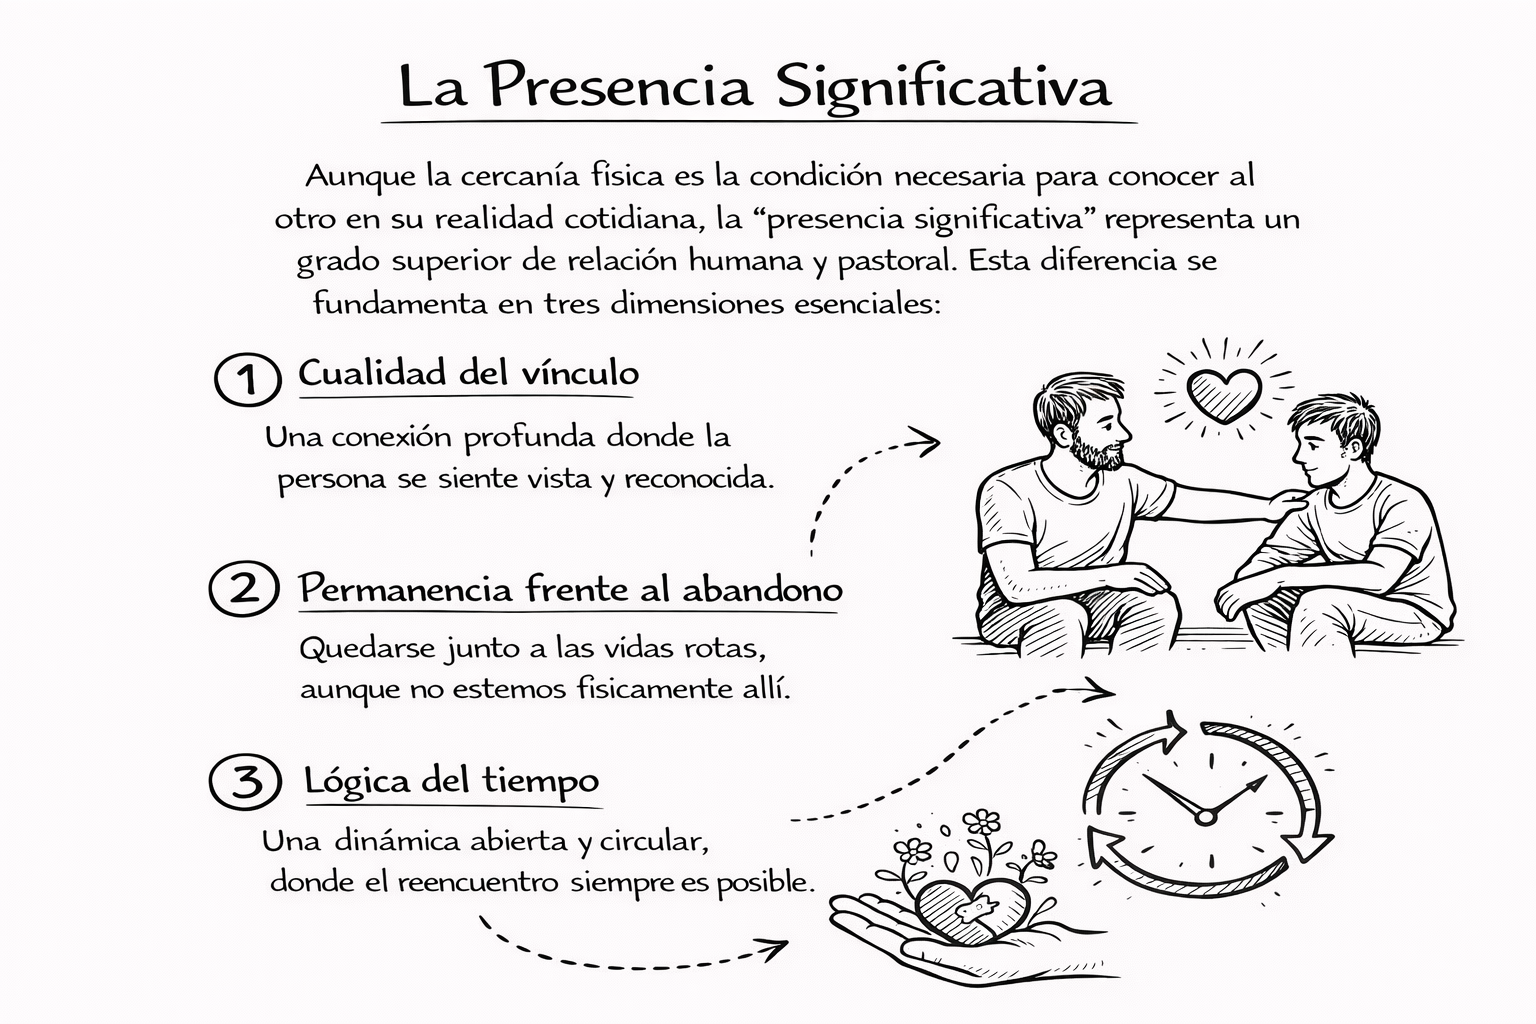
\includegraphics[scale=0.25]{411.png}
		\caption{La presencia significativa}
	\end{figure}
	
	\momento{Fundamento o criterio de discernimiento} \\
	El tiempo califica la cercanía\index{cercanía|textbf} y la convierte en una presencia significativa\index{presencia significativa|textbf}. Esta dimensión constituye una cercanía mucho más honda, de carácter emocional y psicológico, que trasciende la mera coincidencia accidental en un espacio físico determinado.
	
	\momento{Tesis y desarrollo argumental}\\ \\
	Aunque la cercanía física es la condición necesaria para conocer al otro en su realidad cotidiana, la presencia significativa\index{presencia significativa!tres dimensiones}\index{cercanía!y presencia significativa} representa un grado superior de relación humana y pastoral. Esta diferencia se fundamenta en tres dimensiones esenciales:
	\begin{enumerate}
		\item Primero, la cualidad del vínculo, donde la cercanía física puede ser superficial, mientras que la presencia es una conexión profunda que permite que la persona se sienta realmente vista y reconocida.
		\item Segundo, la permanencia frente al abandono, entendiendo que la presencia es la consecuencia de quedarse junto a las vidas más rotas, incluso cuando el acompañante no está físicamente allí.
		\item Tercero, la lógica del tiempo, que abandona la rigidez institucional para adoptar una dinámica territorial y circular, donde el encuentro no termina con un resultado técnico sino que permanece siempre abierto al reencuentro.
	\end{enumerate}
	
	\momento{Respuesta a las objeciones} \\
	\begin{enumerate}
		\item Respecto a la primera objeción, si bien la cercanía física facilita el contacto inicial, para que esta se transforme en presencia significativa debe estar mediada por la ausencia de juicio y la permanencia en el amor.
		\item En cuanto a la segunda objeción, la presencia no se mide por la cantidad de horas técnicas, sino por la capacidad de humanizar el recorrido del hermano, permitiendo que su historia cobre sentido a través de un hilo inespecífico que sostiene su vida.
	\end{enumerate}
	
	\subsection{Artículo 2: Sobre el vínculo (llamar por el nombre) frente a la deshumanización del sistema}
	
	
	\marginnote{Jn 10, 3\label{jn10.3} — \textit{El portero le abre y las ovejas escuchan su voz; él llama a sus ovejas por el nombre}}
	
	\momento{Planteo del tema} \\
	El acto de llamar por el nombre constituye el gesto fundamental para la restauración de la dignidad ontológica en contextos de vulnerabilidad social. Se analiza cómo el vínculo personal y afectivo actúa como un antídoto frente a la tendencia de los sistemas institucionales a fragmentar a la persona, reduciéndola a una cifra, un diagnóstico clínico o una categoría administrativa.
	
	
	
	\momento{Pregunta central} \\
	¿Logra el vínculo, expresado en el acto de llamar por el nombre, romper eficazmente con la dinámica deshumanizadora de los sistemas asistenciales?
	
	\momento{Posturas u objeciones existentes} \\
	\begin{itemize}
		\item Podría argumentarse que el uso del nombre de pila es una formalidad superficial que no altera la eficacia técnica de un tratamiento médico o psicológico. Bajo esta visión, lo que realmente sana es la aplicación de protocolos científicos estandarizados, siendo la cercanía afectiva un elemento secundario.
		\item Otra objeción sostiene que los sistemas deben priorizar el anonimato y la imparcialidad para garantizar la equidad, evitando personalismos que podrían comprometer la objetividad necesaria para gestionar recursos.
		\item Finalmente, se afirma que en situaciones de alta complejidad por consumo de sustancias psicoactivas (SPA), el foco debe estar exclusivamente en la patología, considerando la subjetividad del nombre como algo accesorio frente a la urgencia de la desintoxicación clínica.
	\end{itemize}
	
	\begin{figure}[h]
		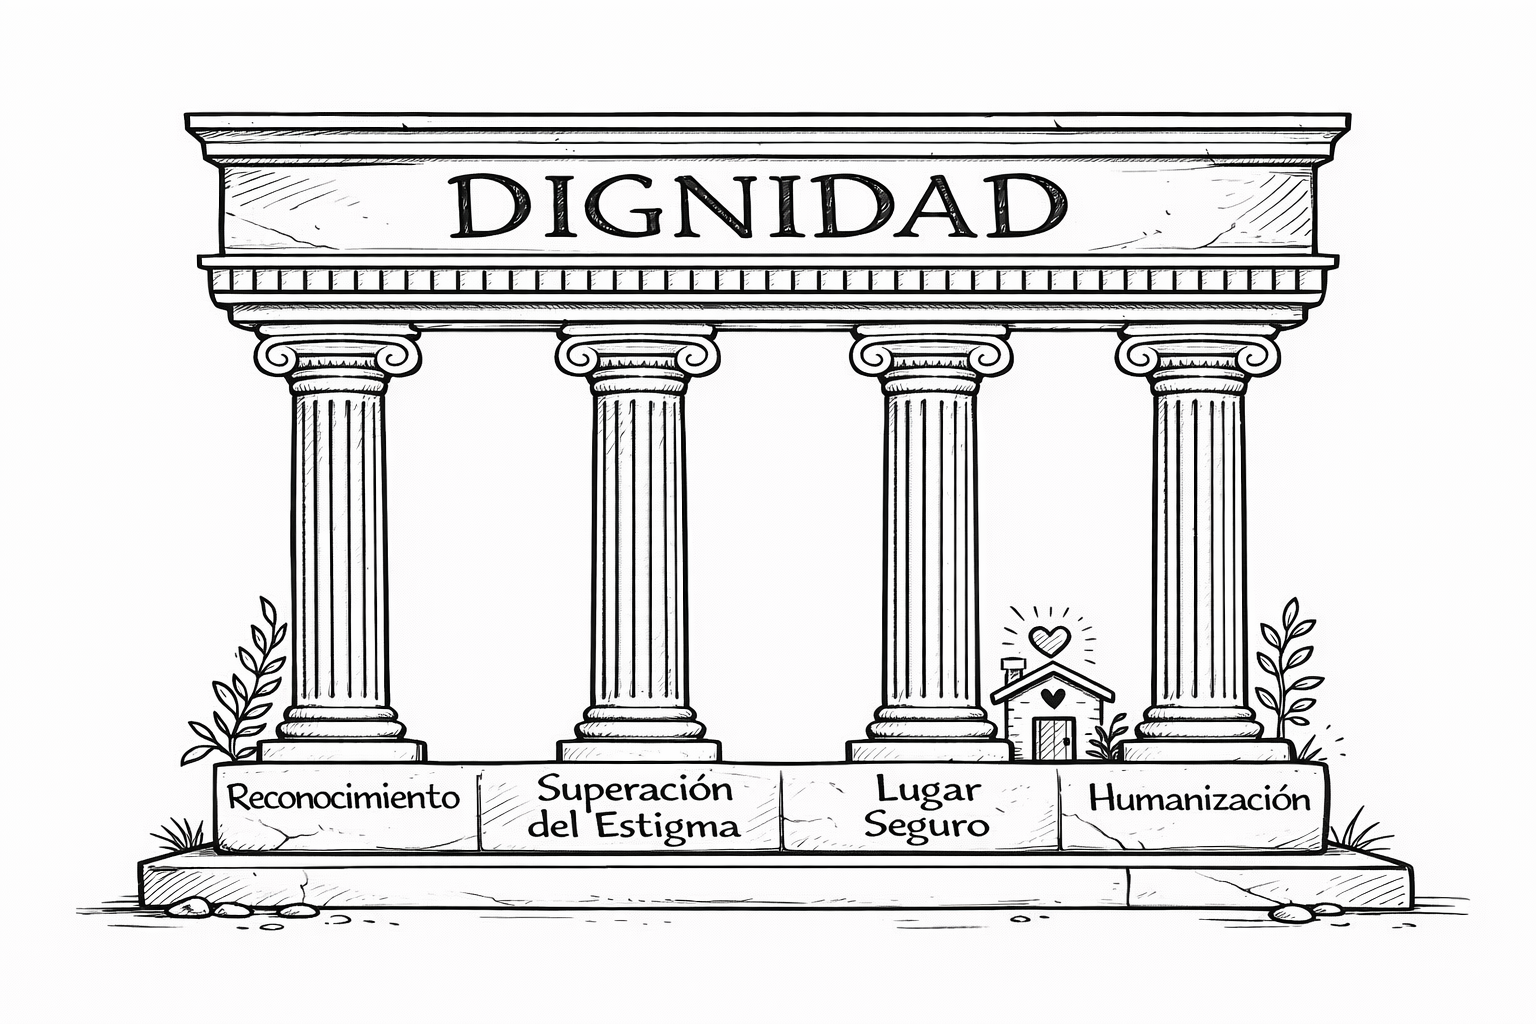
\includegraphics[scale=0.28]{412.png}
		\caption{El vínculo frente a la deshumanización}
	\end{figure}
	
	\momento{Fundamento o criterio de discernimiento} \\
	La antropología cristiana enseña que la persona nunca es un número ni un anónimo, sino un hermano con una dignidad ontológica\index{dignidad!ontológica} que permanece intacta aun cuando su vida esté profundamente herida. El acto de llamar por el nombre reconoce la totalidad del ser y su vocación trascendente, validando que el valor de cada individuo es infinito y sagrado.
	
	
	\momento{Tesis y desarrollo argumental}\\ \\
	El vínculo\index{vínculo|textbf} es el primer paso para reconstruir el lazo social dañado. Mientras que el sistema tiende a la fragmentación administrativa que disecciona al individuo en expedientes o causas penales, el vínculo recupera la unidad de la persona a través de cuatro dimensiones:
	\begin{enumerate}
		\item Primero, el reconocimiento de la dignidad infinita\index{dignidad!infinita}, donde el valor intrínseco no depende de la capacidad de recuperación ni del estado moral.
		\item Segundo, la superación del estigma, reemplazando etiquetas peyorativas por la identidad real del sujeto, lo que permite que la persona se reconozca en sus fortalezas.
		\item Tercero, la construcción de un lugar seguro, donde la confianza generada por el nombre permite que quien ha vivido en el abandono se sienta nuevamente convocado a existir para otros.
		\item Cuarto, la humanización del recorrido, entendiendo que el acompañamiento\index{acompañamiento} no busca solo resultados terapéuticos, sino una atención amante que respeta el carácter artesanal y único de cada proceso de vida.
	\end{enumerate}
	
	\momento{Respuesta a las objeciones} \\
	\begin{enumerate}
		\item Respecto a la primera objeción, si bien la técnica es necesaria, el vínculo es el soporte indispensable que permite que cualquier herramienta profesional sea efectiva; sin amor no hay verdadera sanación ni educación.
		\item En cuanto a la segunda, la verdadera equidad no nace del anonimato burocrático, sino de la misericordia que se hace cargo de la complejidad particular de cada hermano para garantizar su acceso real a derechos.
		\item Finalmente, frente a la tercera objeción, la adicción debe entenderse como un síntoma de una fractura interna y no como la esencia de la persona; reducir al ser humano a su enfermedad es incurrir en un reduccionismo materialista que ignora su unidad integral y su capacidad de ser protagonista de su propia historia.
	\end{enumerate}
	
	\subsection{Artículo 3: Sobre la necesidad de evitar la romantización del barrio}
	
	\momento{Planteo del tema} \\
	El acompañamiento en los territorios exige una mirada honesta que reconozca tanto la potencia sanadora de los vínculos comunitarios como las dinámicas de opresión y pecado social presentes en ellos. Se analiza la importancia de evitar una visión idealizada del barrio para poder identificar y transformar las violencias estructurales que afectan a las personas con consumos problemáticos.
	
	\momento{Pregunta central} \\
	¿Es vital evitar la romantización del barrio en la práctica pastoral de acompañamiento y prevención?
	
	\momento{Posturas u objeciones existentes} \\
	\begin{itemize}
		\item Podría pensarse que el barrio debe ser visto siempre como un santuario de solidaridad y sabiduría popular, y que señalar sus oscuridades sería una falta de respeto a la cultura de los más pobres.
		\item Por otro lado, se argumenta que centrarse en las violencias internas solo refuerza el estigma mediático que ya pesa sobre los sectores populares, por lo que la mirada teórica debería resaltar únicamente los aspectos positivos para contrarrestar los relatos de muerte.
	\end{itemize}
	
	\begin{figure}[h]
		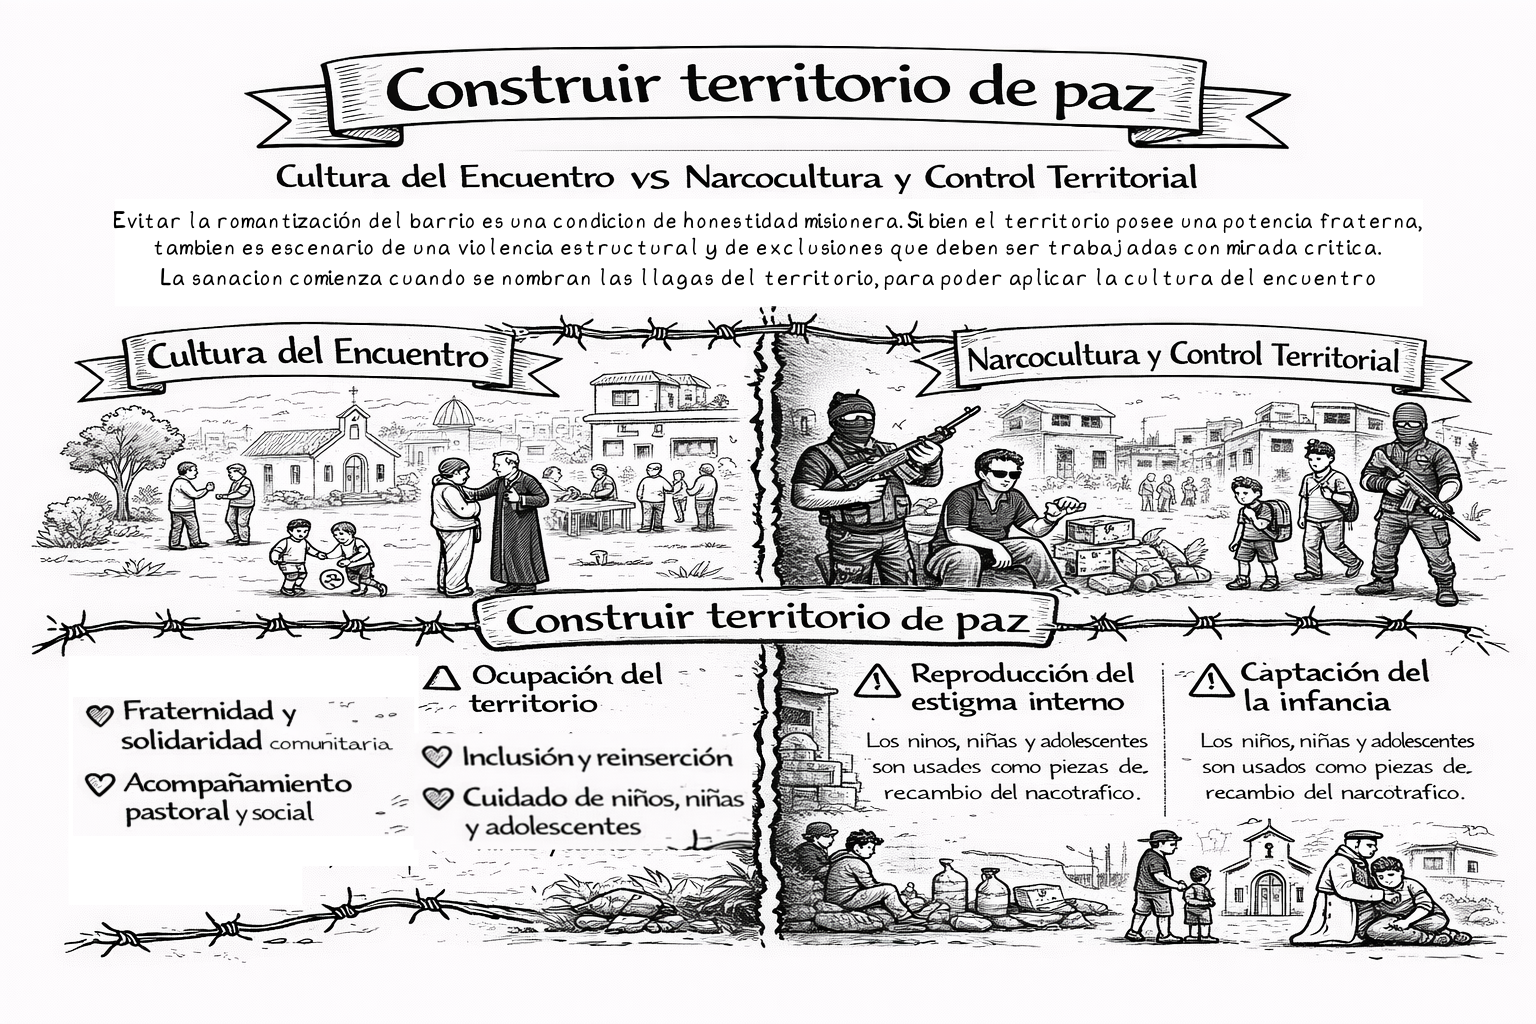
\includegraphics[scale=0.37]{413.png}
		\caption{No hay que romantizar el barrio}
	\end{figure}
	
	\momento{Fundamento o criterio de discernimiento} \\
	Evitar la romantización es una condición de honestidad misionera. Si bien el territorio posee una potencia fraterna, también es escenario de una violencia estructural y de exclusiones que deben ser trabajadas con mirada crítica. La sanación comienza cuando se nombran las llagas del territorio para poder aplicar el fundamento del acompañamiento integral.
	
	\momento{Tesis y desarrollo argumental}\\ \\
	La urgencia de mantener una mirada realista sobre el territorio se fundamenta en cuatro dimensiones teóricas:
	\begin{enumerate}
		\item Primero, la ocupación del territorio por el mal, reconociendo que el narcotráfico no es un agente externo, sino un ente que parasita la economía barrial, secuestra los espacios públicos y utiliza el terror para extinguir las formas de organización comunitaria.
		\item Segundo, la reproducción del estigma interno, donde la propia comunidad puede segregar a los hermanos y hermanas más rotos, a las personas en situación de calle o a la población travesti-trans, tratándolos como desechos.
		\item Tercero, la captación de la infancia, donde el sistema de criminalidad organizada utiliza a niños, niñas y adolescentes como piezas de recambio en la venta de sustancias psicoactivas (SPA), generando una nueva forma de esclavitud.
		\item Cuarto, la identidad de la Iglesia como hospital de campaña\marginnote{\textit{Amoris Laetitia} N°291\label{FALc}}, que exige reconocer que el campo de batalla es doloroso y complejo, demandando una presencia que no ignore el hambre, la falta de derechos ni el desamparo.
	\end{enumerate}
	
	\momento{Respuesta a las objeciones} \\
	\begin{enumerate}
		\item Respecto a la primera objeción, aunque la sabiduría popular es un valor irrenunciable, el discernimiento permite distinguir entre la cultura del pueblo y la narcocultura, la cual lucra con la pobreza y destruye el tejido democrático de la comunidad.
		\item En cuanto a la segunda objeción, el objetivo no es alimentar el estigma, sino ejercer una función profética\index{voz profética} que identifique las violencias reales para que la comunidad organizada pueda exigir el cumplimiento de los derechos fundamentales y construir alternativas de vida que no sean un simple maquillaje de la realidad social.
	\end{enumerate}
	
	\subsection[Artículo 4: Sobre el territorio digital como nuevo desafío]{Artículo 4: Sobre el territorio digital como nuevo desafío social}
	
	
	\momento{Planteo del tema} \\
	El concepto de territorio ha trascendido los límites geográficos tradicionales para abarcar el entorno virtual, donde se desarrolla gran parte de la vida social contemporánea. Este nuevo escenario no debe entenderse simplemente como una herramienta recreativa o de comunicación, sino como un espacio donde se ejerce la ciudadanía digital y se moldea la subjetividad, impactando de forma real en las dimensiones psíquicas y socioemocionales de la persona.
	
	\momento{Pregunta central} \\
	¿Constituye el denominado territorio digital un nuevo escenario de riesgo y un desafío fundamental para el abordaje comunitario de las adicciones?
	
	\momento{Posturas u objeciones existentes} \\
	\begin{itemize}
		\item Podría pensarse que lo digital no califica como territorio al carecer de proximidad física y geografía concreta, perteneciendo únicamente al ámbito de la vida privada.
		\item Asimismo, se argumenta que las redes sociales son herramientas neutrales cuyos riesgos son exagerados por una mirada alarmista.
		\item Finalmente, se sostiene que el verdadero problema reside únicamente en las sustancias químicas, considerando que el uso de pantallas y videojuegos es una actividad inofensiva que no genera daños biológicos comparables al consumo de sustancias psicoactivas (SPA).
	\end{itemize}
	
	\momento{Fundamento o criterio de discernimiento} 
	
	\marginnote{Cfr. Adicciones digitales (cap. 8) y Adicciones comportamentales (cap. 9)}
	
	La existencia y los vínculos se juegan hoy en gran medida en las redes. Este territorio digital es el escenario donde crecen la soledad y nuevas formas de esclavitud que operan sobre los mismos centros de recompensa que las sustancias químicas. Reconocer la ciudadanía digital implica entender que lo virtual tiene un impacto concreto en lo real y en el tejido social.
	
	\momento{Tesis y desarrollo argumental}\\ \\
	El territorio digital representa un desplazamiento de la frontera de intervención pastoral y social. Este desafío se fundamenta en cinco ejes teóricos:
	\begin{enumerate}
		\item Primero, la deslocalización del vínculo y el desarrollo de la subjetividad en la virtualidad. La hiperconexión virtual, paradójicamente, suele profundizar la soledad y deshilachar el tejido social. El tránsito prolongado por espacios digitales naturaliza lógicas de consumo e individualismo que afectan la identidad, la percepción de lo colectivo y la capacidad de sostener encuentros presenciales significativos.
		\item Segundo, los mecanismos de adicción conductual, caracterizados por descargas constantes de dopamina\marginnote{Cfr. art.~\ref{art:dopamina} (Juzgar, Las sustancias y el organismo, La farmacodinámica..., Art. 1...)} a través de un flujo incesante de notificaciones —que pueden alcanzar los centenares diarios—, lo que altera los circuitos cerebrales del placer y la capacidad de espera.
		\item Tercero, el fenómeno del estrés digital y el FOMO (miedo a quedar fuera), que genera una búsqueda de aprobación constante y una hiperconexión que alimenta la ansiedad persistente por la validación de los pares y fragmenta la atención, dificultando el desarrollo de procesos reflexivos profundos.
		\item Cuarto, el surgimiento de nuevas adicciones digitales, como los videojuegos, la pornografía y las apuestas online, que afectan especialmente a los menores de edad y constituyen formas de adicción conductual con mecanismos neurobiológicos análogos a los de las sustancias químicas.
		\item Quinto, el impacto en lo socioemocional y los vínculos de cuidado, donde la exposición desregulada a pantallas —que según estudios internacionales puede superar las ocho horas diarias en adolescentes— reemplaza el silencio reparador y el encuentro presencial, debilitando la función de la familia como puerto seguro y generando una desconexión emocional que invisibiliza los problemas ante los padres hasta que el deterioro es severo.
	\end{enumerate}
	
	\momento{Respuesta a las objeciones} \\
	\begin{enumerate}
		\item Respecto a la primera objeción, lo digital es un territorio porque es el lugar donde el sujeto habita, pasa gran parte de su tiempo y construye su sentido de pertenencia e identidad.
		\item En cuanto a la segunda objeción, la tecnología pierde su neutralidad cuando se convierte en un espacio de deshumanización, manipulación o adicciones digitales como las apuestas online y la pornografía.
		\item Finalmente, frente a la tercera objeción, la ciencia demuestra que las adicciones conductuales comparten mecanismos neurobiológicos con los trastornos por uso de sustancias (TUS), alterando los circuitos de recompensa y generando síntomas de abstinencia como la irritabilidad y la obsesión mental.
	\end{enumerate}
	
	\newpage
	
	\section{La Familia. Estructuras, Familia Comunitaria e Influencias}
	
	Esta sección aborda la familia como la célula vital de la sociedad y la primera experiencia de comunidad, donde el ser humano descubre su dignidad y vocación al amor. Inspirada en la visión de la familia como un poliedro de realidades, se profundiza en el concepto de familia comunitaria\index{familia comunitaria}, entendida como la red de apoyo que ofrece amparo y pertenencia allí donde los vínculos biográficos ---es decir, los lazos familiares de origen--- se encuentran fragilizados. En sintonía con el magisterio del Papa Francisco en Amoris Laetitia\label{FALd}, se reconoce que la familia no es un problema, sino una oportunidad para la integración social y la construcción de un lugar seguro frente al fenómeno del consumo de sustancias psicoactivas (SPA).
	
	Se analizan las influencias macroeconómicas y sociales que condicionan las capacidades de crianza, reconociendo la necesidad de una intervención temprana que permita llegar antes de que el sufrimiento avance. Bajo el paradigma de la crianza comunitaria\index{crianza comunitaria}, esta sección fundamenta teóricamente la corresponsabilidad de todo el tejido social en el cuidado de los niños, niñas y adolescentes, promoviendo una mística de la hospitalidad\index{hospitalidad} que transforma el hogar en una Iglesia doméstica capaz de sanar la orfandad y reconstruir la esperanza en el seno del pueblo.
	
	\subsection{Artículo 1: Sobre la naturaleza y vocación de la familia como oportunidad}
	
	\momento{Planteo del tema} \\
	La familia es frecuentemente analizada desde sus crisis, dificultades o fallas funcionales. Sin embargo, antes de ser un conjunto de problemas a resolver, la familia debe ser comprendida en su realidad fundamental como una comunidad de vida y amor que constituye la base de la sociedad. Se analiza su vocación como un poliedro de relaciones que refleja la dignidad del ser humano.
	
	\momento{Pregunta central} \\
	¿Debe considerarse a la familia principalmente como una fuente de conflictos sociales o como una oportunidad antropológica para la integración y el desarrollo integral?
	
	\momento{Posturas u objeciones existentes} \\
	\begin{itemize}
		\item Podría pensarse que la familia es hoy una institución anticuada, cuya rigidez suele ser la causa de los malestares psíquicos y sociales de sus miembros. Bajo esta visión, la familia sería un recinto de tensiones e intolerancia que dificulta la autonomía individual.
		\item Por otro lado, se argumenta que, ante la diversidad de modelos actuales, el término familia ha perdido su significado unívoco, convirtiéndose en un lugar de paso precario donde los vínculos quedan abandonados a la volubilidad de los deseos.
	\end{itemize}
	
	\momento{Fundamento o criterio de discernimiento} \\
	La familia no es un problema, es principalmente una oportunidad. Como imagen de la Trinidad, es una comunión de personas donde el amor fecundo se convierte en una escultura viviente capaz de manifestar la capacidad creadora y el sentido de trascendencia del ser humano.
	
	\momento{Tesis y desarrollo argumental}\\ \\
	La familia es la célula primera y originaria de la dimensión social de la persona. Su valor esencial se fundamenta en tres pilares teóricos:
	\begin{enumerate}
		\item Primero, la familia como escuela de humanidad, donde el individuo descubre que su identidad se construye en la relación con un otro que lo reconoce y lo ama gratuitamente.
		\item Segundo, la identidad de Iglesia doméstica, donde el espacio vital se transforma en un lugar de presencia compartida, oración y bendición que sostiene la vida cotidiana.
		\item Tercero, el valor del vínculo estable, que ofrece un horizonte definitivo frente a la cultura de lo provisorio, permitiendo que la persona proyecte su futuro con seguridad y confianza.
	\end{enumerate}
	La familia, incluso en su fragilidad, posee la fuerza de amar y enseñar a amar, siendo el ámbito natural donde se custodia la vida en todas sus etapas.
	
	\momento{Respuesta a las objeciones} \\
	\begin{enumerate}
		\item Respecto a la primera objeción, si bien existen familias heridas, la solución no es el debilitamiento del vínculo familiar sino su renovación a través de una pedagogía de la ternura que sane la violencia y el autoritarismo.
		\item En cuanto a la segunda objeción, la verdadera libertad no consiste en el aislamiento individualista, sino en la capacidad de donarse generosamente en un proyecto común que trascienda los caprichos de la sensibilidad para alcanzar la madurez del amor.
	\end{enumerate}
	
	\subsection{Artículo 2: Sobre la familia como escuela de fraternidad y antídoto contra el individualismo}
	
	\momento{Planteo del tema} \\
	En un contexto social caracterizado por el individualismo exasperado y la cultura del descarte, la familia se posiciona como el espacio primordial donde se introduce la fraternidad en el mundo. Se analiza cómo la apertura de la familia hacia la comunidad constituye un eje de prevención fundamental frente a la soledad extrema y el vacío existencial que suelen preceder al consumo de sustancias psicoactivas (SPA).
	
	\momento{Pregunta central} \\
	¿Es la familia un recinto cerrado que debe protegerse de la sociedad o un sujeto activo de transformación social y caridad política\index{caridad política}?
	
	\momento{Posturas u objeciones existentes} \\
	\begin{itemize}
		\item Podría argumentarse que la misión de la familia termina en los límites de su propio hogar, debiendo concentrar todas sus energías en el bienestar de sus miembros biológicos para evitar distracciones de sus deberes primarios.
		\item Asimismo, se sostiene que las familias vulnerabilizadas por la pobreza ya cargan con suficiente peso como para exigírseles una función de acogida o compromiso social con otros, lo que podría debilitar su propia estabilidad interna.
	\end{itemize}
	
	\momento{Fundamento o criterio de discernimiento} \\
	La fraternidad en la familia se irradia como una promesa sobre toda la sociedad. El pensamiento social y eclesial propone que la familia no debe pensarse a sí misma como un recinto llamado a protegerse de la sociedad, sino que debe salir de sí en la búsqueda solidaria, convirtiéndose en un nexo de integración entre lo público y lo privado para hacer doméstico el mundo.
	
	\momento{Tesis y desarrollo argumental}\\ \\
	La familia posee una misión social intrínseca que actúa como un agente de sanación colectiva y prevención de conductas de riesgo. Esta función se despliega en cuatro dimensiones teóricas:
	\begin{enumerate}
		\item Primero, la superación del narcisismo, donde la convivencia enseña a no ser el centro del mundo y a valorar el bien común.
		\item Segundo, la mística de la hospitalidad, que permite a la familia abrir sus puertas a los solos y a los hermanos más rotos, integrándolos en su dinámica cotidiana.
		\item Tercero, el ejercicio de la caridad social, donde el afecto se transforma en un compromiso por la justicia y la defensa de los frágiles, trabajando junto a la comunidad organizada.
		\item Cuarto, la prevención de la orfandad espiritual, ofreciendo un puerto seguro de escucha activa que neutraliza la soledad profunda.
	\end{enumerate}
	Al vivir la fraternidad, la familia deja de ser un mero objeto de asistencia para convertirse en un sujeto con capacidad de transformar las estructuras sociales injustas.
	
	\momento{Respuesta a las objeciones} \\
	\begin{enumerate}
		\item Respecto a la primera objeción, un amor familiar que se encierra exclusivamente en sí mismo corre el riesgo de enfermarse; la verdadera salud del vínculo familiar se encuentra en su capacidad de apertura y entrega gratuita.
		\item En cuanto a la segunda, incluso la familia más herida es capaz de generar vida si se siente parte de un pueblo; la solidaridad mutua entre familias es lo que permite que los hogares no sucumban ante la exclusión, encontrando en la red comunitaria el amparo que los sistemas burocráticos suelen negar.
	\end{enumerate}
	
	\subsection{Artículo 3: Sobre la mística de la hospitalidad como puente hacia lo comunitario}
	
	\marginnote{Heb 13, 2\label{heb13.2} — \textit{No olvidéis la hospitalidad; por ella algunos, sin saberlo, hospedaron a ángeles}}
	
	\momento{Planteo del tema} \\
	La hospitalidad\index{hospitalidad|textbf} no debe entenderse como una simple norma de cortesía social, sino como una mística fundamental que define la identidad de la familia cristiana. Se analiza cómo el gesto de salir de sí y abrir el hogar a la vida herida constituye el puente necesario para transformar la red territorial en una verdadera familia comunitaria\index{familia comunitaria!y hospitalidad}, capaz de alojar a quienes han sido descartados por el sistema.
	
	\momento{Pregunta central} \\
	¿Es la mística de la hospitalidad el fundamento necesario para la existencia de una familia comunitaria en el abordaje de las adicciones?
	
	\momento{Posturas u objeciones existentes} \\
	\begin{itemize}
		\item Podría argumentarse que la hospitalidad es una virtud privada que no tiene impacto en las estrategias de intervención social o sanitaria contra el consumo de sustancias psicoactivas (SPA). Bajo esta visión, la apertura del hogar sería un riesgo innecesario para la seguridad y la intimidad de la familia nuclear.
		\item Asimismo, se sostiene que las instituciones comunitarias deben basarse en protocolos de admisión técnicos y no en una mística de acogida gratuita, la cual resultaría desorganizada e ineficiente frente a la complejidad de la problemática.
	\end{itemize}
	
	\momento{Fundamento o criterio de discernimiento} \\
	El magisterio de Amoris Laetitia\label{FALe} enseña que cuando la familia acoge y sale hacia los demás, especialmente hacia los pobres y abandonados, se convierte en símbolo, testimonio y participación de la maternidad de la Iglesia. La hospitalidad\index{hospitalidad!fundamento en Amoris Laetitia} es el medio por el cual la familia cumple el proyecto de Dios de hacer doméstico el mundo y romper el primer cerco del mortal egoísmo.
	
	\momento{Tesis y desarrollo argumental}\\ \\
	La mística de la hospitalidad\index{hospitalidad!tres dimensiones} se fundamenta como el eje integrador del acompañamiento a través de tres dimensiones esenciales:
	\begin{enumerate}
		\item Primero, el testimonio de la maternidad eclesial, donde la familia que abre sus puertas manifiesta un amor que no pone condiciones y que es capaz de recibir incluso a los hermanos más desastrosos en sus conductas.
		\item Segundo, la humanización del territorio, ya que la hospitalidad transforma el espacio público en un lugar de vecindad y cuidado, neutralizando la soledad extrema que suele anteceder a la adicción.
		\item Tercero, el reconocimiento del rostro de Cristo, donde la acogida gratuita permite valorar la dignidad sagrada del hermano roto, viéndolo como un fin en sí mismo y no como un objeto de asistencia.
	\end{enumerate}
	De este modo, la hospitalidad deja de ser un acto aislado para convertirse en la fuerza que amalgama a los vecinos y las instituciones en una sola familia de familias.
	
	\momento{Respuesta a las objeciones} \\
	\begin{enumerate}
		\item Respecto a la primera objeción, la hospitalidad tiene un impacto real en la salud pública, ya que genera el sentido de pertenencia indispensable para que cualquier proceso de recuperación sea sostenible.
		\item En cuanto a la segunda objeción, una mística de hospitalidad no excluye el orden ni la prudencia, sino que los trasciende; la verdadera eficiencia en contextos de vulnerabilidad no nace de la frialdad burocrática, sino de un amor que sabe recibir la vida como viene para integrarla en un tejido social sanador.
	\end{enumerate}
	
	\subsection[Artículo 4. Sobre el término familia comunitaria]{Artículo 4. Sobre la propuesta del término familia comunitaria}
	
	
	\marginnote{Mc 3, 33-35\label{mc3.33} — \textit{¿Quién es mi madre y quiénes son mis hermanos?... el que cumpla la voluntad de Dios, ese es mi hermano, mi hermana y mi madre}}
	
	\momento{Planteo del tema} \\
	Se propone la incorporación del concepto de familia comunitaria\index{familia comunitaria|textbf} como una categoría fundamental para el abordaje de las adicciones en contextos de exclusión social. Este término busca ampliar la mirada sobre los sistemas de apoyo, reconociendo que la comunidad organizada asume funciones de cuidado y protección que trascienden los vínculos biológicos tradicionales, especialmente allí donde los lazos primarios han sido vulnerados.
	
	\momento{Pregunta central} \\
	¿Es conveniente que el manual proponga el término familia comunitaria en lugar de limitarse exclusivamente a las estructuras familiares tradicionales?
	
	\momento{Posturas u objeciones existentes} \\
	\begin{itemize}
		\item Podría pensarse que el término familia debe reservarse únicamente para los vínculos de parentesco por consanguinidad, matrimonio o adopción, tal como lo definen las ciencias sociales clásicas. Bajo esta visión, ampliar el concepto a lo comunitario podría diluir la responsabilidad específica de los progenitores.
		\item Por otro lado, se argumenta que las redes de apoyo externas, como parroquias o clubes, deben denominarse simplemente instituciones, ya que carecerían de la estabilidad y la intimidad afectiva propias del hogar biográfico.
	\end{itemize}
	
	\momento{Fundamento o criterio de discernimiento} 
	
	\marginnote{Cfr. art. 8.5.3 (familias de acogida)}
	
	La comunidad organizada debe constituirse como la red de apoyo alternativa que ofrece un lugar seguro allí donde los lazos biográficos se encuentran rotos o ausentes. Esta respuesta integral se fundamenta en la mística de la permanencia en el amor y en la identidad de la Iglesia como una familia de familias que no deja a nadie huérfano.
	
	\begin{figure}[h]
		\centering
		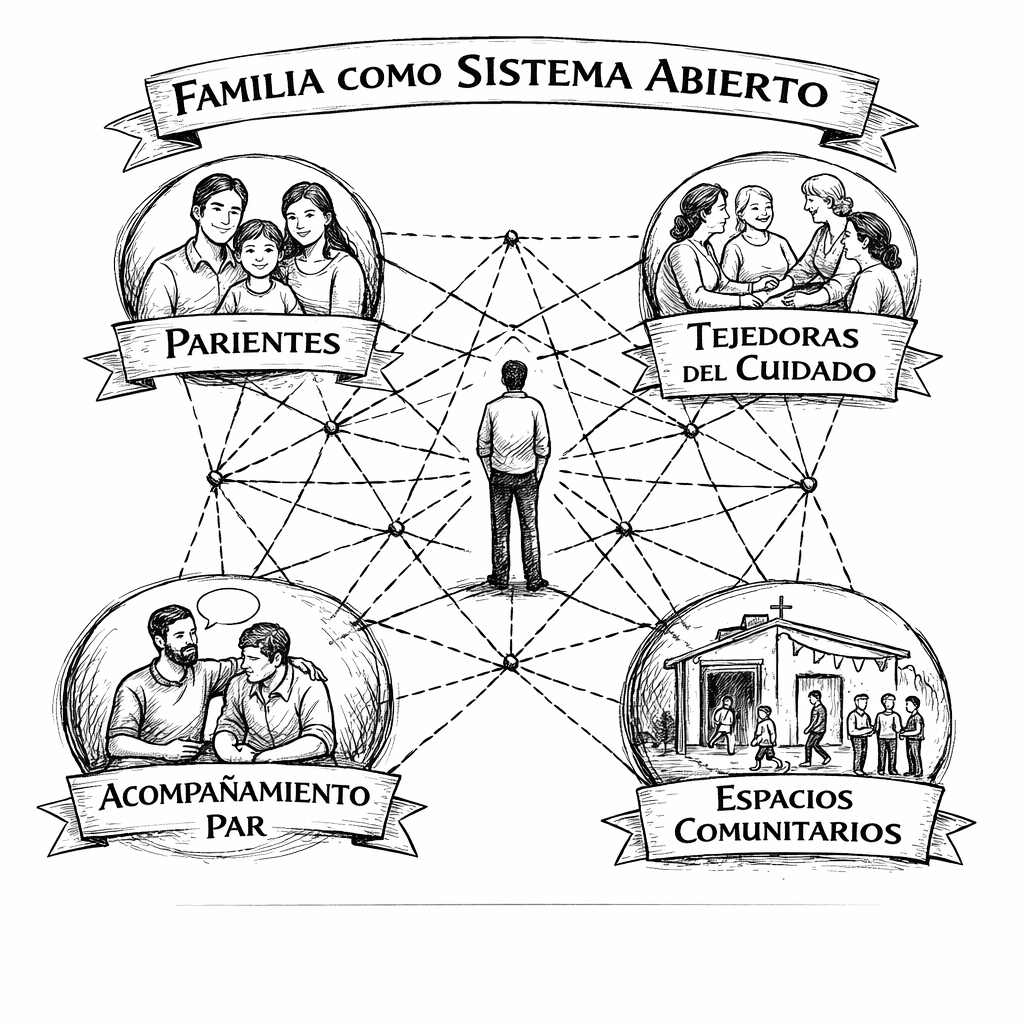
\includegraphics[scale=0.3]{424.png}
		\caption{Familia comunitaria}
	\end{figure}
	
	\momento{Tesis y desarrollo argumental}\\ \\
	La propuesta del término familia comunitaria\index{familia comunitaria!cuatro ejes} responde a un cambio de paradigma necesario fundamentado en cuatro ejes teóricos:
	\begin{enumerate}
		\item Primero, la respuesta a la orfandad funcional, donde la comunidad no solo asiste, sino que ofrece un amparo maternal ante la ruptura de los vínculos primarios.
		\item Segundo, la integración de actores territoriales, conformando una red que une los fragmentos que el sistema administrativo suele separar, actuando como un cuerpo solidario.
		\item Tercero, la construcción de un lugar seguro, un espacio de protección inspirado en el amparo bíblico donde la persona puede ser y al cual siempre puede volver.
		\item Cuarto, la adopción de la crianza compartida, donde todos los miembros del tejido social se sienten corresponsables del desarrollo y la protección de la vida de los hermanos y hermanas más vulnerabilizados por el consumo de sustancias psicoactivas (SPA).
		\item Quinto, la necesidad de protocolos de cuidado y protección. La familia comunitaria\index{familia comunitaria!protocolos de protección} no es un espacio espontáneo que se constituye por el mero deseo de ayudar; requiere una organización responsable que incluya criterios claros de protección de los niños, niñas y adolescentes que participan en ella. La experiencia territorial enseña que la comunidad no es siempre un espacio seguro: el narcotráfico, el abuso y la violencia habitan también en los vínculos de cercanía. Por ello, toda propuesta de familia comunitaria debe incluir pautas de selección y acompañamiento de los referentes adultos, mecanismos de escucha y denuncia accesibles para los menores, y una articulación con los marcos legales de protección de la infancia vigentes en cada país. La mística de la hospitalidad\index{hospitalidad!y responsabilidad institucional} no sustituye la responsabilidad institucional; la encarna y la humaniza.
	\end{enumerate}
	
	\momento{Respuesta a las objeciones} \\
	\begin{enumerate}
		\item Respecto a la primera objeción, el concepto no busca anular la responsabilidad de los padres, sino actuar como un soporte que los fortalece en contextos de estrés extremo, evitando que los niños queden a merced de redes delictivas. Es fundamental distinguir entre complementar la familia —lo cual es deseable y es el objetivo de este concepto— y sustituirla —lo cual, cuando resulta necesario, requiere marcos legales e institucionales formales como la guarda, la tutela o la adopción—. La familia comunitaria\index{familia comunitaria!y familia biológica} opera en el primer registro: acompaña, sostiene y fortalece, pero no reemplaza la responsabilidad parental ni las funciones que el ordenamiento jurídico reserva a las instituciones de protección.
		
		\item En cuanto a la segunda objeción, denominar a estos espacios como instituciones refleja un vínculo meramente funcional; al llamarlos familia, se enfatiza la identidad, el conocimiento por el nombre y la mística de la mesa compartida, transformando la asistencia técnica en un encuentro verdaderamente fraternal.
	\end{enumerate}
	
	\subsection{Artículo 5: Sobre el condicionamiento de las influencias macro en las capacidades de crianza}
	
	\momento{Planteo del tema} \\
	La familia no constituye un compartimento estanco, sino que es un sistema abierto que forma parte de un entramado social más amplio que la condiciona de manera significativa. Se analiza cómo los factores macroeconómicos, políticos y culturales ejercen una presión externa que puede facilitar o, por el contrario, vulnerar el desarrollo humano saludable y las capacidades de cuidado de los referentes familiares.
	
	\momento{Pregunta central} \\
	¿De qué manera las influencias a nivel macro condicionan y afectan las capacidades de crianza en las familias?
	
	\momento{Posturas u objeciones existentes} \\
	\begin{itemize}
		\item Podría pensarse que la crianza es una responsabilidad puramente individual y privada, donde el éxito o fracaso en la educación de los hijos depende exclusivamente de la voluntad y las habilidades personales de los padres, sin que el entorno socioeconómico sea un factor determinante.
		\item Por otro lado, se dice con frecuencia que el amor maternal o paternal es suficiente para superar cualquier adversidad, sugiriendo que incluso en contextos de extrema pobreza o exclusión, las capacidades de cuidado no deberían verse mermadas si existe un vínculo afectivo fuerte.
	\end{itemize}
	
	\momento{Fundamento o criterio de discernimiento} \\
	El magisterio del Papa Francisco en Amoris Laetitia\label{FALf} enseña que es necesario denunciar con franqueza los condicionamientos culturales, sociales y económicos que impiden una auténtica vida familiar. La familia es un bien del cual la sociedad no puede prescindir, y por tanto, el Estado y la comunidad organizada tienen la responsabilidad de garantizar las condiciones necesarias para que los hogares puedan cumplir su misión de cuidar y proteger la vida.
	
	\momento{Tesis y desarrollo argumental}\\ \\
	Las influencias macro impactan en la dinámica familiar a través de cuatro mecanismos teóricos fundamentales:
	\begin{enumerate}
		\item Primero, la privación de recursos básicos, donde la pobreza extrema limita el acceso a la salud y la nutrición, generando cargas adicionales que dificultan el desarrollo motor y cognitivo de los niños, niñas y adolescentes.
		\item Segundo, el estrés crónico del cuidador provocado por la inestabilidad laboral, las jornadas de trabajo excesivamente largas y la falta de servicios esenciales, lo cual agota los recursos psíquicos de los adultos y reduce su disponibilidad emocional para atender las necesidades de sus hijos.
		\item Tercero, la discriminación y exclusión social, que aumentan la respuesta fisiológica al estrés en los padres, debilitando su calidez afectiva y empujando a los jóvenes hacia conductas de riesgo como mecanismo de escape ante la angustia.
		\item Cuarto, la presencia de la criminalidad organizada y el narcotráfico en el territorio, que fragmentan los hogares y obligan a la familia a vivir bajo una lógica de supervivencia que anula los procesos de crianza espontáneos.
	\end{enumerate}
	Ante este escenario, se fundamenta la necesidad de una intervención temprana a través de espacios promocionales comunitarios que actúen como amortiguadores de estas presiones externas.
	
	\momento{Respuesta a las objeciones} \\
	\begin{enumerate}
		\item Respecto a la primera objeción, si bien la responsabilidad individual existe, el ejercicio real de la libertad y la capacidad de educar exigen condiciones mínimas de orden social, jurídico y económico; sin un entorno facilitador, la crianza deja de ser un acto de libertad para convertirse en una lucha reactiva por la subsistencia.
		\item En cuanto a la segunda objeción, el amor es el eje del hogar, pero el estrés prolongado actúa como un perturbador del desarrollo que puede silenciar la respuesta afectiva del cuidador. Por ello, la crianza comunitaria se presenta como la red de apoyo necesaria para sostener a los padres que se encuentran desbordados por las injusticias estructurales.
	\end{enumerate}
	
	\subsection{Artículo 6: Sobre el impacto de la discriminación y la exclusión social en el riesgo de consumo juvenil}
	
	\momento{Planteo del tema} \\
	La vulnerabilidad ante el consumo de sustancias psicoactivas (SPA) no puede explicarse únicamente por factores individuales o biológicos. Existe una estrecha relación entre las dinámicas de exclusión social y los procesos de estigmatización que actúan como potentes fuerzas macroambientales, perturbando el desarrollo saludable de los jóvenes y empujándolos hacia conductas de riesgo como mecanismo de respuesta ante un entorno hostil.
	
	\momento{Pregunta central} \\
	¿De qué manera la discriminación y la exclusión social incrementan la probabilidad de que los jóvenes recurran al consumo de sustancias psicoactivas?
	
	\momento{Posturas u objeciones existentes} \\
	\begin{itemize}
		\item Podría sostenerse que el consumo es una decisión estrictamente individual basada en el libre albedrío, por lo cual la discriminación social no sería una causa sino un pretexto para eludir la responsabilidad personal.
		\item Otra postura argumenta que los factores más determinantes son puramente genéticos, representando la mayor parte de la vulnerabilidad, lo que situaría a la exclusión social como un factor secundario frente a la predisposición orgánica del individuo.
	\end{itemize}
	
	\momento{Fundamento o criterio de discernimiento} \\
	Muchos jóvenes caen en las redes del consumo porque se sienten invisibles y han dejado de existir para otros debido a una cultura del descarte y del abandono. El magisterio enseña que la liberación de las injusticias es lo que promueve verdaderamente la libertad y la dignidad humana, ya que no hay libertad plena allí donde las condiciones sociales asfixian la esperanza.
	
	\momento{Tesis y desarrollo argumental}\\ \\
	La discriminación y la exclusión social operan como detonantes de la vulnerabilidad juvenil a través de tres mecanismos\index{exclusión social!mecanismos} teóricos fundamentales:
	\begin{enumerate}
		\item Primero, el deterioro de la salud mental por estrés crónico, donde la percepción de ser rechazado por el sistema aumenta la respuesta fisiológica de angustia, funcionando la sustancia como un intento autoterapéutico para aliviar una vida percibida como intolerable.
		\item Segundo, el debilitamiento de la red de cuidados, ya que cuando las familias sufren exclusión, los cuidadores manifiestan niveles de agotamiento que afectan sus roles de crianza, dejando a los jóvenes sin el puerto seguro necesario para resistir las presiones del entorno.
		\item Tercero, la invisibilidad y la falta de sentido, donde la exclusión genera una cultura donde el joven siente que no tiene nada que aportar; al carecer de raíces y de un horizonte de oportunidades educativas o laborales, la inmediatez del consumo llena el vacío existencial provocado por el desarraigo social.
	\end{enumerate}
	
	\momento{Respuesta a las objeciones} \\
	\begin{enumerate}
		\item Respecto a la primera objeción, si bien el libre albedrío es un constitutivo humano, su ejercicio real exige condiciones mínimas de justicia social; sin estas, la libertad se ve oscurecida por condicionamientos que necesitan ser sanados mediante la integración comunitaria.
		\item En cuanto a la segunda objeción, aunque la genética es un factor a considerar, la ciencia reconoce que el riesgo es el resultado de una interacción sinérgica entre la biología y el ambiente; un ambiente afectuoso y una comunidad inclusiva pueden proteger incluso a quienes poseen una mayor vulnerabilidad biológica, mientras que la exclusión puede hacer que cualquier individuo cruce el umbral hacia la dependencia.
	\end{enumerate}
	
	\subsection{Artículo 7: Sobre los principios para una intervención preventiva basada en la familia}
	
	\momento{Planteo del tema} \\
	La prevención del consumo de sustancias psicoactivas (SPA) en el ámbito familiar debe superar el modelo asistencialista y meramente informativo para convertirse en un proceso de empoderamiento y fortalecimiento de capacidades. Se analizan los criterios teóricos y metodológicos que permiten que la familia se constituya en un factor de protección eficaz a través del desarrollo de habilidades de cuidado y la consolidación de vínculos saludables.
	
	\momento{Pregunta central} \\
	¿Cuáles son los principios fundamentales que deben regir una intervención preventiva eficaz en el ámbito familiar?
	
	\momento{Posturas u objeciones existentes} \\
	\begin{itemize}
		\item Podría pensarse que la prevención familiar debe ser puramente informativa, bajo la premisa de que si los padres conocen los efectos biológicos y legales de las sustancias y los transmiten a sus hijos, esto bastará para evitar el consumo.
		\item Por otro lado, se argumenta que las intervenciones deben centrarse exclusivamente en los jóvenes, ya que la familia pertenece al ámbito privado y las instituciones no deben interferir en las dinámicas internas de crianza ni en la autonomía del hogar.
	\end{itemize}
	
	\momento{Fundamento o criterio de discernimiento} \\
	El magisterio enseña que la familia es el agente de socialización más profundo y el primer lugar donde se aprende el buen uso de la libertad. Las intervenciones más exitosas son aquellas que logran que los cuidadores desarrollen y practiquen nuevas habilidades con sus hijos, reconociendo que la educación integral es un derecho primario de los padres que la comunidad debe acompañar de forma subsidiaria.
	
	\momento{Tesis y desarrollo argumental}\\ \\
	Una intervención preventiva basada en la familia se fundamenta en seis principios rectores:
	\begin{enumerate}
		\item Primero, la evaluación de necesidades y riesgo, adaptando el programa a la realidad específica de la comunidad, distinguiendo si se requiere una prevención universal, selectiva o indicada.
		\item Segundo, la adecuación a la etapa del ciclo vital y la dosificación, asegurando que las actividades sean apropiadas para la edad de los hijos y cuenten con la permanencia necesaria para automatizar nuevas conductas de cuidado.
		\item Tercero, la metodología interactiva, evitando la charla magistral para fomentar el juego de roles y la participación activa, entendiendo que el aprendizaje social ocurre a través de la práctica guiada.
		\item Cuarto, el desarrollo de la sensibilidad y la estructura, enseñando a los padres a combinar el afecto y la empatía con el establecimiento de reglas claras y supervisión.
		\item Quinto, el vínculo con la escuela y la comunidad organizada, reavivando la alianza educativa para que los cuidadores se involucren en los espacios institucionales del niño, niña o adolescente, fortaleciendo así su red de pertenencia.
		
	\end{enumerate}
	
	\momento{Respuesta a las objeciones} \\
	\begin{enumerate}
		\item Respecto a la primera objeción, la ciencia y la experiencia pastoral demuestran que la mera entrega de información no modifica las conductas; el factor preventivo real es el modelado de hábitos saludables en un ambiente de calidez afectiva.
		\item En cuanto a la segunda objeción, aunque la familia es un núcleo íntimo, no es un compartimento estanco; ante contextos de pobreza o exclusión que generan estrés crónico, la intervención comunitaria es indispensable para sostener la función protectora de los padres bajo la lógica de la crianza compartida.
	\end{enumerate}
	
	\subsection{Artículo 8: Sobre el paradigma de la crianza comunitaria}
	
	\momento{Planteo del tema} \\
	La crianza ha sido tradicionalmente comprendida como una tarea confinada exclusivamente a la esfera de la intimidad familiar y biológica. Sin embargo, ante el deshilachamiento del tejido social provocado por el narcotráfico y la exclusión, surge la necesidad de un cambio de paradigma hacia la crianza comunitaria\index{crianza comunitaria|textbf}. Se analiza cómo la comunidad organizada debe asumir una responsabilidad compartida para proteger y potenciar la vida de los niños, niñas y adolescentes, especialmente cuando los lazos primarios se encuentran fragilizados.
	
	\momento{Pregunta central} \\
	¿Es la crianza comunitaria un modelo legítimo y necesario para garantizar el desarrollo integral y la prevención de conductas de riesgo en contextos de vulnerabilidad?
	
	\momento{Posturas u objeciones existentes} \\
	\begin{itemize}
		\item Podría pensarse que la crianza es una responsabilidad indelegable y privada, por lo que la intervención de otros actores del barrio sería una intromisión en la autonomía familiar. Bajo esta visión, el éxito o fracaso en la educación de un niño depende exclusivamente de sus progenitores, desligando al entorno social de cualquier compromiso ético.
		\item Por otro lado, se argumenta que los espacios comunitarios como clubes o parroquias deben limitarse a brindar servicios específicos (deporte o catequesis) sin involucrarse en los procesos afectivos y de maduración subjetiva de la infancia.
		\item Finalmente, se advierte que involucrar a actores comunitarios en los procesos de crianza podría exponer a los niños, niñas y adolescentes a situaciones de riesgo si esos actores no cuentan con la formación ni la supervisión adecuadas, considerando que los contextos de vulnerabilidad donde se despliega esta propuesta son también escenarios donde operan redes de abuso y explotación.
	\end{itemize}
	
	\momento{Fundamento o criterio de discernimiento} \\
	El magisterio social y la visión de la Iglesia como familia de familias enseñan que el ser humano es constitutivamente relacional. Amoris Laetitia\label{FALg} propone que la familia no debe aislarse, sino ser un nexo de integración entre lo público y lo privado. La comunidad organizada debe constituirse como la red de apoyo que ofrece amparo y pertenencia allí donde la red primaria es inexistente, fundamentándose en el principio de corresponsabilidad social por la vida del hermano.
	
	\momento{Tesis y desarrollo argumental}\\ \\
	La crianza comunitaria se fundamenta como una estrategia de sanación y protección colectiva desplegada en cuatro dimensiones\index{crianza comunitaria!cuatro dimensiones}:
	\begin{enumerate}
		\item Primero, la intervención temprana y promocional, entendiendo que el juego, el deporte y el arte no son solo recreación, sino herramientas preventivas fundamentales que generan fortalezas en la construcción del ser social antes de que el consumo avance.
		\item Segundo, la construcción de un lugar seguro, donde el territorio ofrece espacios de cuidado que neutralizan la oferta de las esquinas y la calle, permitiendo que la infancia recupere su derecho a la alegría.
		\item Tercero, la función de los referentes afectivos comunitarios, quienes ofrecen un apego seguro y una pedagogía de la ternura que repara la orfandad funcional.
		\item Cuarto, la cultura del encuentro\index{cultura del encuentro} frente al individualismo, donde la crianza deja de ser un proceso solitario para convertirse en una dinámica de pueblo que cuida a sus miembros más frágiles, garantizando el acceso a derechos fundamentales que el sistema suele ignorar.
	\end{enumerate}
	
	\momento{Respuesta a las objeciones} \\
	\begin{enumerate}
		\item Respecto a la primera objeción, la crianza comunitaria no busca anular la autoridad de los padres, sino actuar como un soporte subsidiario\index{crianza comunitaria!y subsidiariedad} que los fortalece ante situaciones de estrés extremo o exclusión, evitando que el niño quede a merced de la criminalidad organizada.
		\item En cuanto a la segunda objeción, separar la técnica del afecto es incurrir en una fragmentación deshumanizadora; los espacios comunitarios solo son verdaderamente educativos cuando logran maternar la vida del hermano, transformando la asistencia funcional en un vínculo de pertenencia estable y sanador.
		\item En cuanto a la tercera objeción, la advertencia es legítima y el manual la asume con seriedad. La crianza comunitaria\index{crianza comunitaria!protocolos de protección} no consiste en delegar el cuidado de los menores a cualquier adulto disponible en el territorio. Exige la construcción de entornos protectores con criterios explícitos: selección cuidadosa y formación de los referentes adultos, presencia de más de un adulto en todo espacio de acompañamiento de menores, canales de escucha y denuncia accesibles para los niños, articulación con los organismos de protección de derechos de la infancia de cada país, y una cultura institucional que no tolere ni encubra ninguna forma de maltrato o abuso. La Iglesia ha aprendido dolorosamente que la cercanía y el afecto, cuando no están acompañados de protocolos claros y transparencia, pueden convertirse en el escenario del peor de los daños. La crianza comunitaria que este manual propone asume esa lección como parte constitutiva de su diseño, no como un agregado posterior.
	\end{enumerate}
	
	\newpage
	
	\section{El trabajo y el dinero}
	
	Esta sección se propone discernir la dimensión operativa del ser humano como un componente intrínseco de su salud y su dignidad ontológica. El trabajo no se analiza aquí como un simple dato de subsistencia económica, sino como el eje vertebrador que permite al hermano reconstruir su identidad, ordenar su tiempo y participar activamente en la obra creadora de Dios. Asimismo, se busca iluminar la relación con el dinero y los recursos materiales, entendiéndolos como un signo de realismo y un termómetro de la madurez alcanzada frente a la dinámica de la compulsión. A través de este juicio pastoral, buscaremos integrar la laborterapia, el aprendizaje de oficios y el empleo remunerado bajo el criterio de una misericordia estructurada que promueva la autonomía y el protagonismo del sujeto en su pueblo.
	
	\subsection{Artículo 1: El trabajo como participación en la creación}
	
	\marginnote{Gn 2, 15\label{gen2.15} — \textit{Tomó el Señor Dios al hombre y lo puso en el jardín del Edén para que lo cultivara y lo cuidara}}
	
	\momento{Planteo del tema} La cultura contemporánea tiende a reducir la labor humana a una mera mercancía o a un simple instrumento de producción de riqueza. En el acompañamiento de nuestros hermanos, resulta vital rescatar el sentido profundo del quehacer diario. No se trata solo de qué produce el hombre, sino también de qué hace el trabajo con el hombre. Debemos discernir si la actividad laboral es un elemento accidental o si es una dimensión sagrada que permite al sujeto desplegar su vocación y perfeccionar su naturaleza en diálogo con el Creador.
	
	\momento{Pregunta central} ¿Constituye el trabajo una dimensión esencial de la identidad humana que permite a las personas participar de la obra creadora de Dios y restaurar su dignidad herida?
	
	\momento{Posturas u objeciones existentes}
	\begin{itemize}
		\item Parece que el trabajo es únicamente una carga necesaria para la supervivencia biológica o una consecuencia del desorden del mundo que no posee un valor espiritual ni terapéutico intrínseco.
		\item Parece que, en personas con problemas de adicción, el trabajo es un objetivo inalcanzable o un premio que solo debe otorgarse al final del recorrido, considerándolo ajeno a las etapas iniciales de la sanación.
		\item Parece que la labor operativa o técnica es inferior a la vida espiritual, sugiriendo que la verdadera recuperación se juega solo en el plano de la fe o de la psicología, dejando la dimensión del hacer en un plano secundario.
		
	\end{itemize}
	
	\momento{Fundamento o criterio de discernimiento} Nuestra antropología cristiana y el magisterio social enseñan que el ser humano, creado a imagen de Dios, es llamado a ser colaborador de la obra divina a través del cultivo y cuidado de la creación. El trabajo es el eje vertebrador que otorga sentido a la vida cotidiana. Al trabajar, el ser humano no solo transforma las cosas, sino que se realiza a sí mismo como sujeto capaz y creativo.
	
	\momento{Tesis y desarrollo argumental} Respondemos que el trabajo es un componente intrínseco de la salud integral y un motor de la identidad operativa por las siguientes razones:
	\begin{itemize}
		\item Espejo de la identidad: A través de su obra, el ser humano se reconoce a sí mismo como alguien que tiene algo para dar. La labor permite objetivar los propios talentos y reconstruir una subjetividad fragmentada por la despersonalización que genera el consumo.
		\item Ordenador del tiempo y del deseo: El trabajo estructura el ritmo diario, combatiendo los bloques de tiempo vacío que suelen ser disparadores de la compulsión. Educa la voluntad hacia metas concretas y permite transitar de la gratificación inmediata a la satisfacción del esfuerzo compartido.
		\item Protagonismo en el pueblo: Al trabajar, el individuo sale de su aislamiento y se integra en la comunidad, pasando de ser un objeto de asistencia a ser un sujeto activo que contribuye al bien de su familia y de su barrio.
	\end{itemize}
	
	\momento{Respuesta a las objeciones}
	
	\begin{enumerate}
		\item A la primera: Aunque el trabajo implique esfuerzo y fatiga, su esencia es promocional y humanizante. Es el camino por el cual el hombre perfecciona la creación y encuentra un propósito que trasciende la mera supervivencia.
		\item A la segunda: El trabajo, bajo la forma de laborterapia, es un medicamento desde el inicio del proceso. No es un premio al éxito, sino una herramienta pedagógica que ayuda a recuperar la autovaloración y los hábitos necesarios para la vida.
		\item A la tercera: No existe una división real entre lo espiritual y lo operativo. En la projimidad de la tarea diaria, la persona encuentra una vía de sanación concreta donde la fe se hace carne y el espíritu se fortalece a través de la disciplina y el servicio.
	\end{enumerate}
	
	\subsection{Artículo 2: Las 3T (Tierra, Techo y Trabajo)}
	
	\marginnote{Lc 4, 18-19\label{lc4.18} — \textit{El Espíritu del Señor está sobre mí... me envió a anunciar a los pobres la Buena Noticia, a proclamar la libertad a los cautivos}}
	
	\momento{Planteo del tema} La dignidad del ser humano no puede sostenerse en el vacío; requiere de condiciones materiales básicas que permitan el despliegue de su libertad y su pertenencia a un pueblo. Siguiendo el magisterio social de la Iglesia, identificamos tres pilares fundamentales para una vida digna: Tierra, Techo y Trabajo. Resulta necesario juzgar si estos elementos son demandas puramente políticas o si constituyen dimensiones sagradas de justicia restaurativa, cuya ausencia alimenta el desamparo estructural en el que se instalan las adicciones.
	
	\momento{Pregunta central} ¿Constituyen la Tierra, el Techo y el Trabajo una tríada indisoluble de derechos sagrados cuya garantía es condición necesaria para una recuperación integral y sostenible?
	
	\momento{Posturas u objeciones existentes}
	\begin{enumerate}
		\item Parece que la Iglesia debe centrarse únicamente en la dimensión espiritual de la persona humana, dejando las demandas de Tierra, Techo y Trabajo a los organismos estatales o a la lucha política, social y técnica.
		\item Parece que, ante la urgencia de la adicción, lo único prioritario es la abstinencia, considerando que la falta de vivienda o de propiedad de la tierra son problemas secundarios que se resolverán una vez que el sujeto esté \textit{limpio}.
		\item Parece que proponer el acceso a las 3T como parte del tratamiento es una forma de asistencialismo que fomenta la dependencia del hermano en lugar de su autonomía y esfuerzo personal.
	\end{enumerate}
	
	\momento{Fundamento o criterio de discernimiento} El pensamiento social de la Iglesia enseña que la dignidad humana es integral y que los bienes de la creación están destinados a todos. No existe verdadera libertad sin una base material que la sustente. Tierra, Techo y Trabajo son derechos sagrados porque permiten que la persona deje de ser un errante descartado para transformarse en un ciudadano con raíces, protección y propósito. El desamparo que produce la falta de estas dimensiones es el caldo de cultivo donde la narcocultura ofrece sus falsas promesas.
	
	\momento{Tesis y desarrollo argumental} Respondemos que la garantía de las 3T es un imperativo de justicia y un motor de resiliencia por las siguientes razones:
	\begin{itemize}
		\item Tierra como pertenencia: El acceso a un territorio y a una comunidad organizada permite que el hermano recupere su sentido de hogar. La tierra simboliza las raíces y la estabilidad necesarias para proyectar un futuro que el consumo suele fragmentar en un presente perpetuo.
		\item Techo como protección: El techo no es solo una estructura física, sino el espacio de intimidad y seguridad donde se reconstruye el vínculo familiar. Sin un lugar seguro donde descansar y ser recibido, la persona permanece en un estado de alerta biológica y estrés crónico que dispara el deseo de consumo.
		\item Trabajo como sostenimiento: El trabajo es el eje que permite que la Tierra y el Techo se vuelvan sostenibles. Es el motor que devuelve al sujeto su lugar en la economía popular y su protagonismo social, impidiendo que caiga nuevamente en la deriva de la exclusión.
	\end{itemize}
	
	\momento{Respuesta a las objeciones}
	\begin{enumerate}
		\item A la primera: Una espiritualidad que ignore la carne sufriente y las carencias materiales del hermano es una fe desencarnada. La misión eclesial incluye la caridad política, que busca transformar las estructuras de pecado que niegan estos derechos fundamentales.
		\item A la segunda: La abstinencia\index{abstinencia|textbf} es frágil si no está custodiada por una vida digna. Las 3T no son el premio al final de la meta, sino el andamiaje de justicia que permite que el hermano se sostenga en pie frente a las presiones del entorno y la marginalidad.
		\item A la tercera: El acceso a las 3T no es asistencialismo, sino restitución de derechos. No se trata de <<dar>> de forma pasiva, sino de generar las condiciones para que el hermano, mediante su propio protagonismo y el apoyo de la comunidad, pueda habitar su tierra, cuidar su techo y dignificarse en su trabajo.
	\end{enumerate}
	
	\subsection{Artículo 3: La Misericordia Estructurada}
	
	\momento{Planteo del tema} En el acompañamiento de personas con trayectorias de consumo y exclusión, surge con frecuencia una tensión entre la acogida incondicional y la necesidad de un orden operativo. Existe el riesgo de caer en un asistencialismo que, por evitar la exigencia, termina abandonando al hermano en su propio caos. Se trata de discernir si la implementación de normas, horarios y responsabilidades laborales es un acto contrario a la caridad o si, por el contrario, constituye una forma superior de amor que ofrece al sujeto el andamiaje necesario para reconstruir su voluntad.
	
	\momento{Pregunta central} ¿Es la misericordia estructurada un criterio pastoral legítimo que une la ternura de la acogida con la firmeza de la regla pedagógica como condición necesaria para la salud integral del hermano?
	
	\momento{Posturas u objeciones existentes}
	\begin{enumerate}
		\item Parece que la misericordia debe ser siempre incondicional y sin límites, por lo que establecer reglas o estructuras de trabajo sería una forma de legalismo que contradice la gratuidad del amor evangélico.
		\item Parece que las estructuras rígidas y la exigencia de tareas replican los sistemas de control y castigo que ya han expulsado al hermano de otros ámbitos sociales, profundizando su sentimiento de rechazo.
		\item Parece que, frente al dolor del otro, lo único pastoral es la flexibilidad total, considerando que cualquier tipo de estructura es una carga insoportable para quien ya está suficientemente quebrado.
	\end{enumerate}
	
	\momento{Fundamento o criterio de discernimiento} La verdadera misericordia no es un sentimiento difuso ni una permisividad que deja al otro a la deriva. Es una caridad operante que se hace cargo de la fragilidad ajena proveyendo un entorno seguro y predecible. Una misericordia sin estructura es desidia; una estructura sin misericordia es crueldad. El equilibrio reside en una pedagogía que utiliza la firmeza de la regla para proteger la libertad que aún está débil, ofreciendo un \textit{hospital de campaña}\index{hospital de campaña!y misericordia estructurada} donde ambos, el afecto y el orden, son necesarios.
	
	\momento{Tesis y desarrollo argumental} Respondemos que la misericordia estructurada es un instrumento de justicia y sanación por las siguientes razones:
	\begin{itemize}
		\item Seguridad vincular y contención: Para quien viene del caos de la calle o de la compulsión, el límite sano\index{límite sano|textbf} funciona como un abrazo protector. La estructura del trabajo y las normas comunitarias reducen la ansiedad al ofrecer un escenario donde el hermano sabe qué se espera de él y qué puede esperar del entorno.
		\item Reparación de la voluntad: La adicción desestructura la capacidad de decidir. La misericordia estructurada propone pequeñas metas diarias que permiten entrenar nuevamente el músculo de la voluntad, transformando la inercia en una intencionalidad orientada al bien.
		\item El valor pedagógico del límite: El límite no es un castigo, sino una frontera que define el espacio de respeto mutuo. Enseña que las propias acciones tienen consecuencias y que el error es una oportunidad de aprendizaje y perdón, no un motivo de expulsión definitiva.
	\end{itemize}
	
	\momento{Respuesta a las objeciones}
	\begin{enumerate}
		\item A la primera: La gratuidad de Dios no es desorden. La misericordia estructurada transparenta un amor que quiere que el hermano crezca y se perfeccione. El límite es la expresión de un Dios que nos cuida impidiendo que nos autodestruyamos.
		\item A la segunda: A diferencia de los sistemas punitivos, la estructura pastoral nace del vínculo y la projimidad. No se impone desde una autoridad lejana, sino que se vive en comunidad, donde quien acompaña se somete a la misma regla y ritmo de vida que quien es acompañado. El límite se pone pensando en el bien del otro, y por amor.
		\item A la tercera: La flexibilidad total a menudo se convierte en indiferencia. Proponer una estructura es un signo de esperanza: es decirle al hermano que creemos en su capacidad de responder, de ser responsable y de protagonizar su propio proceso de vida nueva.
	\end{enumerate}

	\subsection[Artículo 4: Gradualidad del trabajo en la recuperación]{Artículo 4: El sentido gradual del trabajo en la recuperación}
	
	\momento{Planteo del tema} Una de las tensiones más recurrentes en los dispositivos de acompañamiento es la incorporación de la actividad laboral. Existe el temor de que el trabajo represente un estrés excesivo que dispare una recaída o que, por el contrario, la inactividad prolongada fomente la desestructuración del sujeto. Debemos discernir si la exigencia de trabajar es adecuada para alguien que está sanando sus vínculos y su voluntad, evitando caer en simplificaciones que ignoran la complejidad de la vida de la persona en recuperación.
	
	\momento{Pregunta central} ¿Deben las personas que transitan un proceso de recuperación realizar actividades laborales?
	
	\momento{Posturas u objeciones existentes}
	\begin{enumerate}
		\item Parece que no deben trabajar, ya que el estrés propio del mercado laboral y la presión por la productividad son disparadores de ansiedad que ponen en riesgo la abstinencia recién alcanzada.
		\item Parece que el trabajo debe ser un premio que se otorga solo al final del recorrido, una vez que la persona ha demostrado una madurez absoluta, considerando que antes sería una distracción del proceso terapéutico y espiritual.
		\item Parece que cualquier ocupación es válida con tal de mantener a la persona ocupada, sugiriendo que la naturaleza de la tarea no importa siempre que sirva para combatir los bloques de tiempo vacío que deja el consumo.
	\end{enumerate}
	
	\momento{Fundamento o criterio de discernimiento} Respondemos que para contestar adecuadamente esta pregunta es imperativo precisar que, en el ámbito de la pastoral de adicciones, el trabajo no es un concepto unívoco. Hablar de trabajo implica referirse a tres dimensiones distintas y progresivas que deben aplicarse según la madurez del sujeto: la laborterapia como medicina del hábito, el aprendizaje de oficios como reconstrucción de la identidad operativa y el trabajo remunerado como hito de justicia y autonomía social.
	
	\momento{Tesis y desarrollo argumental} Se afirma que la persona en recuperación debe trabajar, siempre que la actividad se ajuste artesanalmente a la etapa que atraviesa su corazón y su mente, bajo los siguientes criterios:
	\begin{itemize}
		\item El trabajo que organiza (Laborterapia): En las fases iniciales, el fin no es la productividad sino la reorganización de la vida interior. Las tareas cotidianas de la comunidad funcionan como un instrumento pedagógico para recuperar ritmos, disciplina y sentido de servicio. Es el paso del caos del consumo al orden de lo compartido.
		\item El trabajo que capacita (Aprender un oficio): Superada la crisis inicial, el hermano necesita redescubrir sus talentos. Esta etapa formativa busca que el sujeto adquiera competencias técnicas y habilidades sociales. Aprender un oficio devuelve la esperanza y permite al hermano proyectar un futuro posible fuera del circuito de la exclusión.
		\item El trabajo que integra (Empleo remunerado): Finalmente, la inserción laboral real es el signo de la recuperación plena. El salario es el motor que permite la independencia económica y familiar. El trabajo remunerado verifica que el hermano ha dejado de ser un objeto de asistencia para transformarse en un ciudadano protagonista de su propio pueblo.
	\end{itemize}
	
	\momento{Respuesta a las objeciones}
	\begin{enumerate}
		\item A la primera: El riesgo de recaída se mitiga mediante la gradualidad. La laborterapia no busca la exigencia del mercado, sino la contención emocional en un entorno protegido. Es una estructura que cuida la libertad del hermano mientras esta se fortalece.
		\item A la segunda: El trabajo no es la meta final, sino una dimensión constitutiva de la salud desde el inicio. Posponer lo operativo hasta el final priva al hermano de un motor de identidad esencial. La inclusión laboral debe ser un eje transversal que acompañe todo el recorrido de sanación.
		\item A la tercera: No cualquier ocupación sana. El trabajo debe tener un sentido pedagógico y respetar la dignidad de la persona. Una actividad vacía de propósito no contribuye a la reconstrucción del ser, mientras que una tarea realizada con mística comunitaria restaura la autoestima herida.
	\end{enumerate}
	
	\subsection{Artículo 5: El dinero como signo de realismo y madurez}
	
	\momento{Planteo del tema} En los procesos de acompañamiento, la relación de las personas con el dinero suele ser un tema de alta sensibilidad. Existe una tendencia a considerar los recursos materiales como un factor de riesgo absoluto que debe evitarse para prevenir recaídas, o como un elemento ajeno a la vida espiritual y terapéutica. Sin embargo, omitir la dimensión económica del sujeto puede conducir a una recuperación desencarnada que no prepara al hermano para las exigencias del mundo real. Debemos discernir si el manejo de los recursos materiales es un obstáculo para la sanación o si constituye una herramienta pedagógica necesaria para medir la madurez frente a la compulsión.
	
	\momento{Pregunta central} ¿Debe integrarse el manejo del dinero en el proceso de recuperación como un signo de realismo y un termómetro de la madurez frente a la dinámica de la impulsividad?
	
	\momento{Posturas u objeciones existentes}
	\begin{enumerate}
		\item Parece que las personas en recuperación no deben manejar dinero, ya que disponer de efectivo actúa como un disparador inmediato del deseo de consumo (craving) y aumenta exponencialmente las probabilidades de una recaída.
		\item Parece que la pastoral de adicciones debe centrarse exclusivamente en los valores del espíritu y la salud mental, considerando que la preocupación por el dinero contamina la naturaleza del proceso y desvía al hermano de su verdadera sanación interior.
		\item Parece que el manejo de recursos solo debe permitirse en la etapa final de egreso institucional, asumiendo que cualquier contacto previo con el dinero es una imprudencia que pone en riesgo los logros alcanzados en el tratamiento.
	\end{enumerate}
	
	\momento{Fundamento o criterio de discernimiento} El realismo antropológico enseña que el ser humano es una unidad biopsicosocial y espiritual que vive en un mundo condicionado por necesidades materiales. La libertad auténtica no consiste en la huida de la realidad, sino en la capacidad de habitarla con responsabilidad. El manejo del dinero, bajo un esquema de acompañamiento, permite verificar el paso del patrón compulsivo (gratificación inmediata) al patrón de planificación (proyección vital). Sin este ejercicio de realismo, la autonomía recuperada corre el riesgo de ser una ilusión que se quiebra al primer contacto con el mercado.
	
	\momento{Tesis y desarrollo argumental} Respondemos que la integración del manejo del dinero es indispensable para una salud integral y sostenible por las siguientes razones:
	\begin{itemize}
		\item El dinero como termómetro de madurez: La capacidad de conservar y administrar recursos sin ceder al impulso de consumo es la verificación objetiva de que el \textit{freno} biológico y espiritual ha comenzado a funcionar. Es el terreno donde se entrena la voluntad para distinguir entre el deseo momentáneo y la necesidad real.
		\item Reeducación financiera y planificación: Quien viene de la exclusión o de la calle suele vivir en un presente perpetuo donde el recurso se agota instantáneamente. Utilizar el dinero de forma pedagógica —especialmente el primer sueldo— enseña al hermano a proyectar, a ahorrar para su familia y a cuidar su casa común, devolviéndole su identidad de administrador responsable.
		\item Superación de la orfandad material: El acceso y la gestión del dinero rompen la lógica de la dependencia institucional. Manejar recursos propios devuelve la dignidad al sujeto, permitiéndole pasar de ser un asistido pasivo a ser un protagonista que contribuye al sostenimiento de su hogar y de su comunidad organizada.
	\end{itemize}
	
	\momento{Respuesta a las objeciones}
	\begin{enumerate}
		\item A la primera: El riesgo no se elimina con la prohibición, sino que se gestiona con la pedagogía. El manejo acompañado del dinero en entornos seguros permite que el hermano aprenda a convivir con el estímulo sin ser gobernado por él, fortaleciendo su autoeficacia antes de la inserción total.
		\item A la segunda: No hay división entre la fe y la carne. Una espiritualidad sana es la que ayuda al hombre a ser libre en medio de sus circunstancias. El dinero, ordenado al bien de la familia y el servicio, deja de ser un motor de esclavitud para transformarse en un medio de justicia.
		\item A la tercera: Posponer el contacto con el dinero hasta el final genera un choque de realidad que suele ser devastador. La exposición gradual y tutorizada es el andamiaje necesario para que el hermano gane seguridad y desmitifique la fascinación que el consumo ha proyectado sobre el recurso material.
	\end{enumerate}
	
	\newpage
	
	\section{Superación de la Fragmentación e Integralidad del Acompañamiento}
	
	Esta sección aborda el desafío fundamental de superar la fragmentación\index{acompañamiento!integralidad} en el abordaje de los consumos problemáticos, analizando tanto su dimensión epistemológica como administrativa. Se examina cómo la especialización excesiva del conocimiento y la compartimentación burocrática de las instituciones suelen deshumanizar a la persona, reduciéndola a un conjunto de problemas aislados\index{fragmentación} que el sistema no logra integrar. Frente a este escenario, se propone el acompañamiento inespecífico como la fuerza integradora y el hilo conductor que hilvana las respuestas de la salud, la justicia y lo social.
	
	El texto fundamenta teóricamente la centralidad de la persona\index{integralidad!centralidad de la persona} como un eje transversal que exige un cambio de lógica: pasar de la autosuficiencia institucional a un trabajo en red horizontal. Bajo esta mirada integral, se destaca el papel de la comunidad organizada como el ámbito capaz de alojar la complejidad del sujeto, brindando un puerto seguro y un vínculo de pertenencia que trasciende la asistencia técnica. Finalmente, se analiza la importancia de promover procesos de integración que reconozcan la dignidad ontológica de cada hermano y hermana, asegurando que el acceso a derechos fundamentales no se vea obstaculizado por la rigidez de los sistemas administrativos fragmentados.
	
	\subsection{Artículo 1: Sobre la fragmentación epistemológica y administrativa}
	
	\momento{Planteo del tema} \\
	El abordaje de las adicciones enfrenta el obstáculo de la fragmentación, un fenómeno que opera tanto en la construcción del conocimiento como en la organización de las respuestas institucionales. Esta división desarticula la unidad de la persona, dificultando una intervención que responda a la complejidad real de quienes atraviesan un consumo problemático de sustancias psicoactivas (SPA).
	
	\momento{Pregunta central} \\
	¿En qué consiste la fragmentación epistemológica y administrativa y de qué manera afecta la dignidad y la accesibilidad en el acompañamiento integral?
	
	\momento{Posturas u objeciones existentes} \\
	\begin{itemize}
		\item Podría argumentarse que la especialización del conocimiento es estrictamente beneficiosa, ya que la profundidad en áreas como la medicina, la psicología o el derecho garantiza una atención técnica de mayor calidad.
		\item Asimismo, se sostiene que la división de funciones en el Estado es la forma más eficiente de gestionar los recursos públicos, evitando el desorden mediante carteras con presupuestos y competencias específicas. Bajo esta visión, la fragmentación no sería un problema, sino un requisito de la modernidad técnica y administrativa.
	\end{itemize}
	
	\begin{figure}[h]
		\centering
		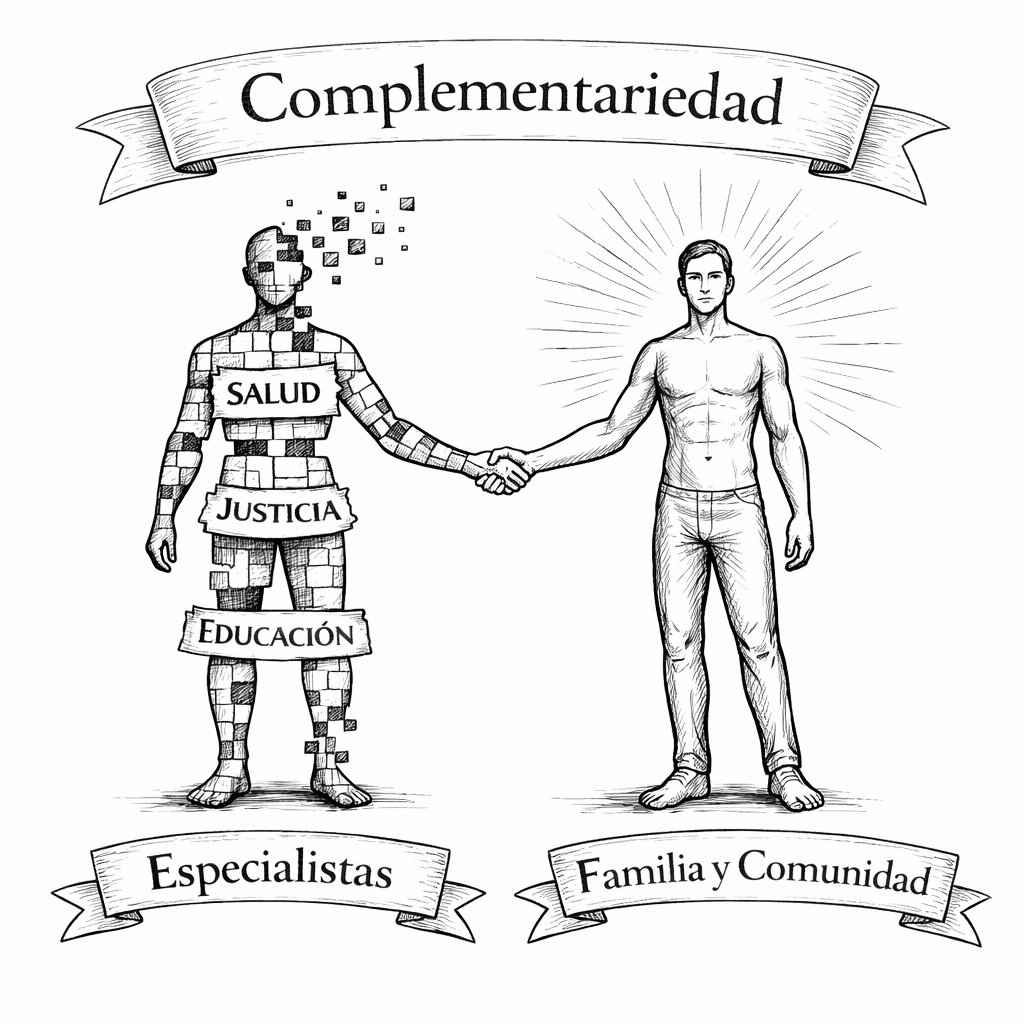
\includegraphics[scale=0.3]{431.png}
		\caption{La fragmentación y la mirada integral}
	\end{figure}
	
	\momento{Fundamento o criterio de discernimiento} \\
	El pensamiento integral y el magisterio social enseñan que el todo es más que la suma de las partes. Una respuesta fragmentada resulta insuficiente para abordar problemas complejos, ya que la hiperespecialización y la burocracia suelen ignorar la unidad ontológica de la persona. La técnica debe estar siempre subordinada a una mirada holística, capaz de reconocer la totalidad de la vida del otro.
	
	\momento{Tesis y desarrollo argumental}\\ \\
	La fragmentación actúa como un doble obstáculo que deshumaniza\index{fragmentación|textbf} la atención:
	\begin{enumerate}
		\item Primero, la fragmentación epistemológica disecciona al ser humano a través de un efecto de lupa; la ciencia se especializa tanto en una parte (biológica, psíquica o social) que pierde de vista la historia personal, la soledad y los vínculos territoriales del sujeto.
		\item Segundo, la fragmentación administrativa traduce esta división en casillas institucionales estancas. Los gobiernos se organizan en compartimentos con competencias limitadas que no logran articularse, de modo que los requisitos de una institución pueden convertirse en impedimentos para otra. Esta realidad genera una crisis de accesibilidad donde las personas más vulnerabilizadas quedan excluidas, al no poder navegar por sí mismas un entramado institucional que las percibe como un conjunto de trámites aislados y no como una vida que clama por ser integrada.
	\end{enumerate}
	
	\momento{Respuesta a las objeciones} \\
	\begin{enumerate}
		\item Respecto a la primera objeción, si bien la especialización permite profundidad, en el paradigma de la complejidad la interacción entre las dimensiones de la persona produce realidades que no pueden comprenderse estudiando cada pieza por separado.
		\item En cuanto a la segunda objeción, la eficiencia administrativa se pierde cuando la respuesta es ineficaz para el sujeto; la verdadera eficiencia nace de una red que, superando la autosuficiencia, logre unificar los fragmentos de respuesta para humanizar el recorrido de cada hermano.
	\end{enumerate}
	
	\subsection{Artículo 2: Sobre la acción del acompañamiento inespecífico frente a la fragmentación}
	
	\momento{Planteo del tema} \\
	Frente a la deshumanización que produce la división de la persona en áreas técnicas aisladas, surge la necesidad de una figura integradora. Se analiza el acompañamiento inespecífico como el hilo conductor que atraviesa las diversas instancias de atención, devolviendo la unidad a la vida del hermano y garantizando que el sistema no lo expulse.
	
	\momento{Pregunta central} \\
	¿Es el acompañamiento inespecífico el medio eficaz para superar la fragmentación administrativa y epistemológica en el abordaje de las adicciones?
	
	\momento{Posturas u objeciones existentes} \\
	\begin{itemize}
		\item Podría pensarse que el acompañamiento debería ser siempre específico y técnico para ser profesional. Bajo esta visión, si una persona tiene un problema de salud, necesita exclusivamente un médico, y si tiene un problema legal, un abogado; por tanto, un acompañante inespecífico carecería de las herramientas necesarias para resolver problemas concretos.
		\item Por otro lado, se argumenta que la fragmentación es un problema de gestión estatal que debe resolverse mediante reformas burocráticas y unificación de presupuestos, y no a través de una acción comunitaria basada en vínculos afectivos.
	\end{itemize}
	
	\begin{figure}[h]
		\centering
		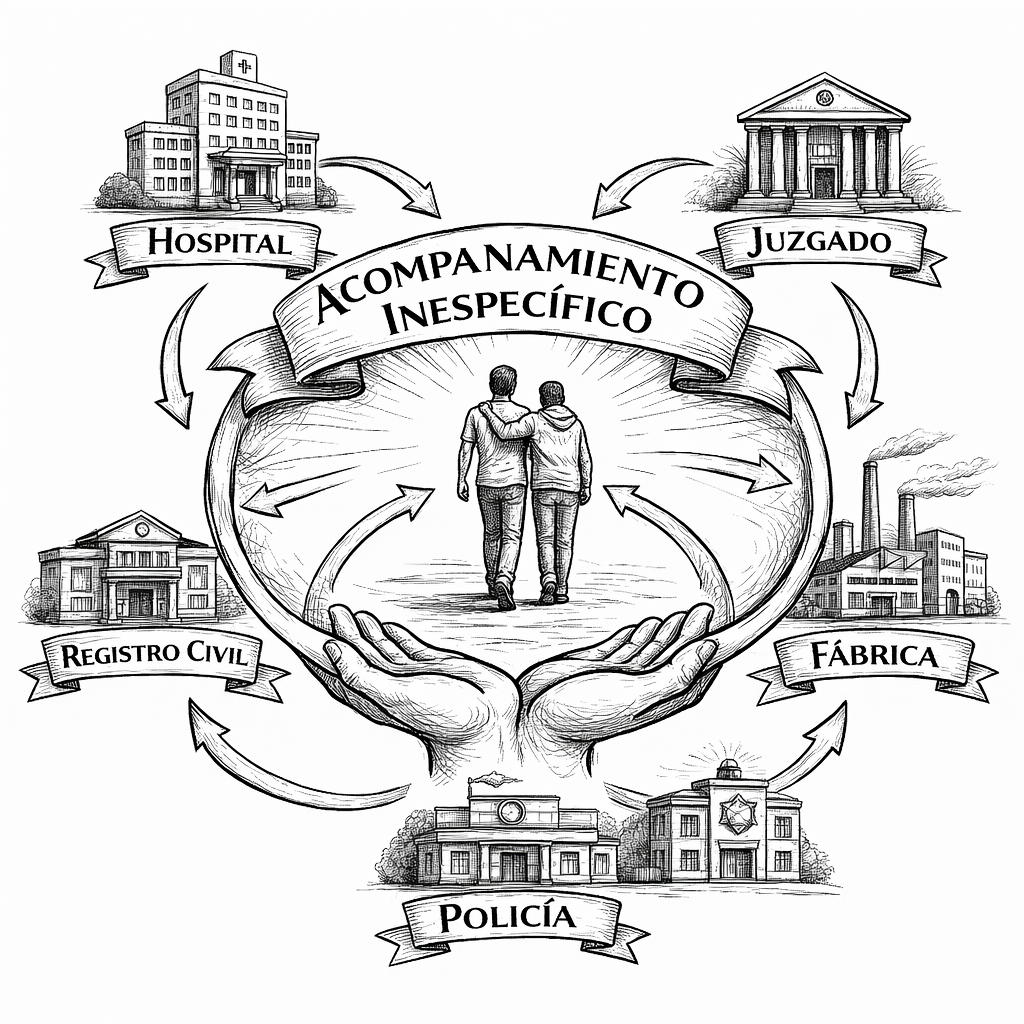
\includegraphics[scale=0.3]{432.png}
		\caption{El acompañamiento inespecífico de la comunidad}
	\end{figure}
	
	\momento{Fundamento o criterio de discernimiento} \\
	El acompañamiento\index{acompañamiento|textbf} se define como la humanización del recorrido. Mientras que el especialista tiene una mirada incisiva pero parcial, el acompañante comunitario posee una mirada holística e integral, similar a la de una madre que conoce la totalidad de la vida de su hijo y es capaz de unir lo que el sistema separa.
	
	\momento{Tesis y desarrollo argumental}\\ \\
	El acompañamiento inespecífico\index{acompañamiento inespecífico|textbf} actúa como la fuerza integradora del proceso de recuperación a través de tres funciones fundamentales:
	\begin{enumerate}
		\item Primero, la humanización del recorrido, permitiendo que el sujeto supere el miedo y la falta de sentido frente a instituciones que suelen ser frías y expulsivas.
		\item Segundo, la transversalidad del proceso, ya que, a diferencia del abordaje técnico que es coyuntural y puntual, el acompañamiento inespecífico va de la mano de la persona en todas sus etapas, ya sea en la calle, el hospital o el juzgado.
		\item Tercero, el hilado de los fragmentos, donde el acompañante actúa como el soporte que une las respuestas de salud, identidad y justicia, garantizando la accesibilidad real a los derechos fundamentales que la división administrativa suele obstaculizar. Esta presencia inespecífica es lo que permite que los intentos de cambio de una persona se transformen en una historia de vida con sentido.
	\end{enumerate}
	
	\momento{Respuesta a las objeciones} \\
	\begin{enumerate}
		\item Respecto a la primera objeción, el acompañamiento inespecífico no busca reemplazar al saber técnico, sino complementarlo; su función es asegurar que la persona pueda sostener el tratamiento médico o el proceso legal mediante el soporte emocional y la presencia constante.
		\item En cuanto a la segunda objeción, aunque el Estado es el garante de derechos, carece de la capacidad de generar comunidades de cuidado y vínculos de pertenencia; solo la comunidad organizada puede ofrecer el lugar seguro y la persistencia en el amor indispensables para una sanación integral.
	\end{enumerate}
	
	\subsection{Artículo 3: La horizontalidad y centralidad de la persona en el trabajo en red}
	
	\momento{Planteo del tema} \\
	El trabajo en red suele verse obstaculizado por visiones jerárquicas o enfoques centrados únicamente en la sustancia. Se analiza la necesidad de estructurar las redes de acompañamiento de forma horizontal, situando la singularidad de la persona como el eje transversal que unifica todas las intervenciones institucionales y comunitarias.
	
	\momento{Pregunta central} \\
	¿Por qué el trabajo en red en el abordaje de las adicciones debe estructurarse de forma horizontal y situar a la persona como eje central de toda acción?
	
	\momento{Posturas u objeciones existentes} \\
	\begin{itemize}
		\item Podría pensarse que el trabajo en red debe ser estrictamente jerárquico y piramidal, donde las instituciones del Estado o los especialistas médicos dicten directivas a las comunidades para asegurar el control administrativo de los recursos.
		\item Asimismo, se dice con frecuencia que el enfoque inicial debe estar centrado exclusivamente en la eliminación del síntoma (la abstinencia), dejando el abordaje de la subjetividad y la historia personal para una etapa posterior a la recuperación biológica.
	\end{itemize}
	
	\momento{Fundamento o criterio de discernimiento} \\
	Para actuar en red la construcción debe ser horizontal, poniendo en valor lo que cada sector puede aportar. El desplazamiento del enfoque debe ir siempre del consumo a la persona, reconociendo que el ser humano es una unidad integral —biopsicosocial y espiritual— y que la red debe responder a esa totalidad para que la sanación sea sostenible.
	
	\momento{Tesis y desarrollo argumental}\\ \\
	La horizontalidad y la centralidad de la persona se fundamentan en cuatro dimensiones teóricas:
	\begin{enumerate}
		\item Primero, la superación de la autosuficiencia institucional, reconociendo que nadie tiene todas las respuestas y que el complemento de saberes (ONG, parroquia, hospital, club) beneficia realmente al sujeto.
		\item Segundo, la valoración de todos los aportes, donde la red permite que la suma de voluntades resulte en un bien mayor que la simple adición de las partes, planificando estrategias en términos de procesos y no de eventos aislados.
		\item Tercero, el respeto a la singularidad y los tiempos, lo que obliga a la red a adoptar una mirada artesanal que se adapte a la historia sagrada de cada hermano, evitando imponer recetas o estándares rígidos de éxito.
		\item Cuarto, la promoción del protagonismo, donde la red no asiste a un objeto pasivo, sino que empodera a un sujeto responsable, integrando a los acompañantes pares y a la comunidad como actores políticos de transformación social.
	\end{enumerate}
	
	\momento{Respuesta a las objeciones} \\
	\begin{enumerate}
		\item Respecto a la primera objeción, aunque la técnica es necesaria, el Estado y las instituciones no pueden generar por sí solos vínculos de pertenencia; la horizontalidad protege la autonomía de la comunidad y evita que el saber territorial sea absorbido por una lógica burocrática.
		\item En cuanto a la segunda objeción, un enfoque centrado solo en la sustancia es un reduccionismo que ignora la complejidad de la persona; situar al sujeto en el centro desde el inicio humaniza el recorrido y garantiza que la red institucional no lo trate como un caso administrativo que rebota entre oficinas.
	\end{enumerate}
	
	\newpage
	
	\section{Metodología de la Ternura y Roles Comunitarios}
	
	Esta sección profundiza en la metodología de la ternura\index{metodología de la ternura|textbf} como eje central del abordaje comunitario, integrando la pedagogía de los tres lenguajes propuesta por el Papa Francisco: la cabeza para comprender la complejidad del fenómeno, el corazón para la afectividad que lee el dolor en los ojos, y las manos para el tacto y el abrazo que derriban los muros del estigma. Se describen roles fundamentales nacidos del territorio, como las madrazas —mujeres referentes de la comunidad que asumen un rol maternal de cuidado y protección allí donde los vínculos primarios están rotos— y los acompañantes pares, expertos por experiencia que, habiendo transitado el mismo dolor, se convierten en líderes positivos capaces de guiar a otros desde la empatía y la autoridad del testimonio.
	
	A través del paradigma de la crianza comunitaria, este enfoque propone una amistad con el tiempo que rechaza las recetas estandarizadas y apuesta por procesos artesanales basados en la reciprocidad, el enraizamiento y la convicción de que los vínculos humanos son el motor definitivo para la restauración de la dignidad. Bajo esta mirada, se enfatiza la importancia de llegar antes mediante la intervención temprana, potenciando los espacios promocionales como el juego, el arte y el deporte. Estos ámbitos son entendidos como una gimnasia para la definición del ser social, fundamentales para generar fortalezas subjetivas antes de que el consumo avance. Finalmente, la metodología de la ternura reconoce que la dignidad ontológica de la persona permanece intacta aun en lo más oscuro de la adicción, siendo tarea de la comunidad organizada remover los obstáculos que bloquean el despliegue del espíritu.
	
	\subsection{Artículo 1: La aplicación de los tres lenguajes en la metodología de la ternura}
	
	\momento{Planteo del tema} \\
	El abordaje comunitario de las adicciones requiere una pedagogía que trascienda la mera transmisión de información técnica o moral. Se analiza la propuesta del Papa Francisco sobre la integración de los tres lenguajes —la cabeza, el corazón y las manos— como la estructura fundamental de una metodología de la ternura que permita un encuentro real y transformador con la vida herida.
	
	\momento{Pregunta central} \\
	¿De qué manera deben integrarse y aplicarse los lenguajes de la cabeza, el corazón y las manos en el acompañamiento integral de las personas con consumos problemáticos?
	
	\momento{Posturas u objeciones existentes} \\
	\begin{itemize}
		\item Podría pensarse que el abordaje debe ser estrictamente técnico e intelectual, centrándose exclusivamente en el conocimiento científico y teórico del fenómeno para garantizar la eficacia del tratamiento (solo la cabeza).
		\item Asimismo, se sostiene con frecuencia que los gestos físicos o afectivos, como el abrazo o el contacto cercano (las manos), son secundarios o poco profesionales en un entorno de salud mental, debiendo priorizarse la instrucción moral o la intervención farmacológica.
	\end{itemize}
	
	\begin{figure}[h]
		\centering
		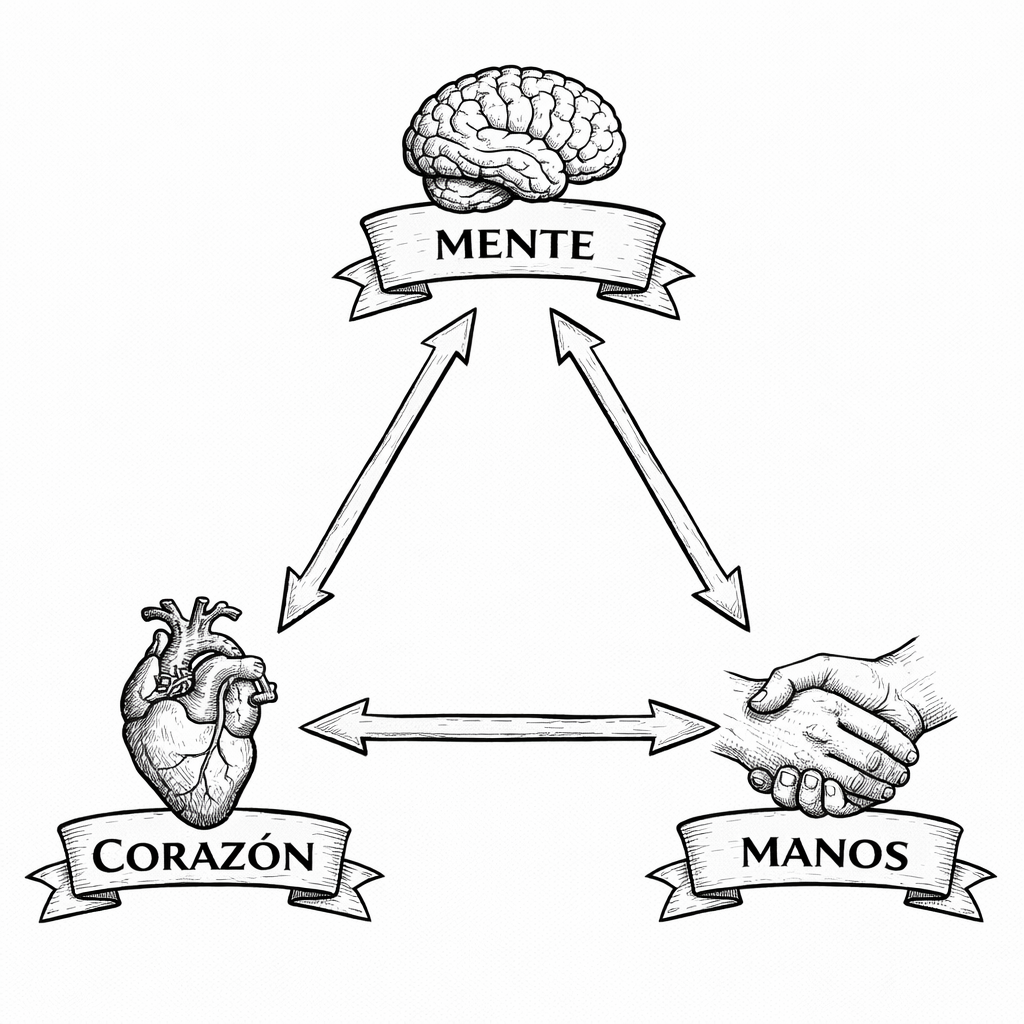
\includegraphics[scale=0.3]{441.png}
		\caption{Metodología de la ternura}
	\end{figure}
	
	\momento{Fundamento o criterio de discernimiento} \\
	La antropología cristiana y el magisterio de Francisco enseñan que la persona es una unidad indivisible. La metodología de la ternura\index{metodología de la ternura!definición|textbf} no es un sentimentalismo, sino una forma de transparentar el amor de Dios que sale al encuentro de la totalidad del ser humano, reconociendo que no hay verdadera sanación sin una cercanía que involucre el pensamiento, el afecto y la acción concreta.
	
	\momento{Tesis y desarrollo argumental}\\ \\
	La aplicación de los tres lenguajes constituye una pedagogía integral que humaniza el proceso de recuperación y supera el estigma social a través de tres dimensiones interconectadas:
	\begin{enumerate}
		\item Primero, el lenguaje de la cabeza, que implica el desarrollo de estrategias creativas para comprender la complejidad de las sustancias psicoactivas (SPA), traduciendo el saber en herramientas y habilidades accesibles para las personas acompañadas.
		\item Segundo, el lenguaje del corazón, referido a la afectividad y la proximidad emocional; consiste en la capacidad de leer el dolor en los ojos y la sonrisa del hermano, brindándole la seguridad de que es valorado por su dignidad ontológica por encima de su problema.
		\item Tercero, el lenguaje de las manos, que representa el cuerpo y el tacto indispensables para derribar los muros de la indiferencia. Gestos como dar la mano o el abrazo devuelven la dignidad al cuerpo sufriente de Cristo en el pueblo y transforman el territorio en un lugar de amparo.
	\end{enumerate}
	La conjunción de estos elementos permite reconocer la radical singularidad de cada hermano y acompañar su vida tal como viene.
	
	\momento{Respuesta a las objeciones} \\
	\begin{enumerate}
		\item Respecto a la primera objeción, aunque la técnica es necesaria, un abordaje que solo use la cabeza resulta insuficiente para quienes sufren de orfandad y soledad extrema; la verdadera sabiduría pastoral exige que la mente se involucre con el sentir y el hacer para sanar integralmente.
		\item En cuanto a la segunda objeción, el lenguaje de las manos no es una distracción del tratamiento, sino un gesto de inclusión y respeto que a menudo posee un impacto terapéutico superior a los discursos, ofreciendo una seguridad inmediata a quien ha vivido años de descarte y rechazo social.
	\end{enumerate}
	
	\subsection{Artículo 2: La amistad con el tiempo como eje de la recuperación}
	
	\momento{Planteo del tema} \\
	Se analiza la amistad con el tiempo como una virtud fundamental y eje estratégico del abordaje comunitario. A diferencia de las lógicas institucionales que exigen resultados inmediatos, este enfoque reconoce que la sanación de vidas atravesadas por el consumo de sustancias psicoactivas (SPA) requiere procesos lentos, circulares y respetuosos de la historia sagrada de cada persona.
	
	\momento{Pregunta central} \\
	¿Por qué se considera que la amistad con el tiempo es el eje fundamental y la virtud principal de la recuperación en el modelo comunitario?
	
	\momento{Posturas u objeciones existentes} \\
	\begin{itemize}
		\item Podría pensarse que el tiempo es un recurso escaso y que, ante la urgencia de las sobredosis y la violencia del narcotráfico en los territorios, la recuperación debe ser inmediata y eficiente, pues esperar demasiado tiempo podría interpretarse como negligencia o falta de profesionalismo en el tratamiento.
		\item Por otro lado, se sostiene con frecuencia que el tiempo de recuperación debe estar dictado estrictamente por protocolos científicos y administrativos —como la duración de una beca o periodos fijos de internación—, considerando que si no hay resultados en ese lapso, el proceso es un fracaso.
	\end{itemize}
	
	\momento{Fundamento o criterio de discernimiento} \\
	El magisterio del Papa Francisco enseña que el tiempo es superior al espacio, lo cual implica que es prioritario iniciar procesos de maduración humana más que intentar dominar espacios de control. «El tiempo le gana a todo» y la Iglesia y la comunidad deben ser amigas del tiempo, alejándose de una lógica de «franquicia» para abrazar procesos vitales lentos y profundos.
	
	\momento{Tesis y desarrollo argumental}\\ \\
	La amistad con el tiempo es el eje de la recuperación comunitaria porque reconoce que la sanación de una vida rota no es un evento técnico, sino un proceso existencial que no puede ser forzado. Esta tesis se fundamenta en cinco dimensiones teóricas:
	\begin{enumerate}
		\item Primero, la superación de la lógica de franquicia, entendiendo que la construcción de vínculos no puede estandarizarse y requiere permanencia para generar la confianza necesaria.
		\item Segundo, la distinción entre el tiempo biográfico y el institucional, donde el acompañamiento comunitario debe durar lo que la vida necesite, sin las fechas de vencimiento propias de los sistemas administrativos.
		\item Tercero, el respeto por el proceso artesanal, donde se camina al lado de la persona respetando sus idas y vueltas, entendiendo que forzar un cambio genera resistencia.
		\item Cuarto, el hacer historia a través de la escucha, donde la presencia cariñosa y prolongada funciona como un depósito de la memoria que da sentido al recorrido del hermano.
		\item Quinto, el contrapunto a la inmediatez del consumo, ofreciendo un paso lento que enseña a manejar la frustración y la espera, reconstruyendo la capacidad de proyectar un futuro frente a la satisfacción mágica del instante que propone la adicción.
	\end{enumerate}
	
	\momento{Respuesta a las objeciones} \\
	\begin{enumerate}
		\item Respecto a la primera objeción, la urgencia de la crisis se atiende con la presencia constante y no con soluciones apresuradas; el tiempo no es un retraso, sino el escenario donde la misericordia se vuelve carne para una sanación sostenible.
		\item En cuanto a la segunda objeción, los éxitos en el territorio no se miden por altas médicas en plazos rígidos, sino por el fortalecimiento de la dignidad ontológica y la reintegración en una familia o comunidad; un proceso que parece lento para el Estado puede ser el único milagro real capaz de torcer una historia de muerte hacia una vida con sentido.
	\end{enumerate}
	
	\subsection{Artículo 3: El paradigma de «llegar antes» y la potencia de los espacios promocionales}
	
	\marginnote{Lc 19, 5\label{lc19.5} — \textit{Zaqueo, baja en seguida, porque hoy tengo que alojarme en tu casa}}
	
	\momento{Planteo del tema} \\
	Históricamente, el abordaje de los consumos problemáticos ha sostenido 
	un fuerte sesgo asistencial, centrando la mirada y los recursos en los 
	procesos de acompañamiento cuando el sufrimiento y la adicción ya han 
	avanzado. «Llegar antes» no es una ingenuidad sobre la omnipresencia de 
	las sustancias en la sociedad de consumo: es la decisión estratégica de 
	priorizar la presencia formativa sobre la reaccional, de estar en la vida 
	de la persona antes de que la crisis instale el acompañamiento como único 
	modo posible. Frente a este enfoque reactivo, surge la necesidad de 
	consolidar el paradigma de la intervención temprana, fundamentado en la 
	capacidad de la comunidad organizada para generar escenarios que 
	contribuyan a forjar fortalezas en la construcción subjetiva y colectiva 
	de la niñez y la adolescencia.
	
	\momento{Pregunta central} \\
	¿Cuál es el valor estratégico de «llegar antes» a través de espacios promocionales en el marco de una metodología de la ternura y la prevención integral?
	
	\momento{Posturas u objeciones existentes} \\
	\begin{itemize}
		\item Podría pensarse que actividades como el juego, el deporte o el arte son recursos meramente recreativos, accesorios o secundarios, careciendo de un valor preventivo real frente a la potencia de las sustancias psicoactivas (SPA). Bajo esta visión, se suele decir que la energía pastoral y los presupuestos del Estado deberían reservarse exclusivamente para las instancias de crisis, desintoxicación o atención en situación de calle.
		\item Asimismo, existe la postura de que la prevención debe ser estrictamente informativa o técnica, centrada en advertir sobre los daños biológicos de la droga, y no en el desarrollo integral del ser social.
	\end{itemize}
	
	\momento{Fundamento o criterio de discernimiento} \\
	El magisterio del Papa Francisco y la antropología cristiana enseñan que la identidad del joven se forja en el encuentro con el otro. La metodología de la ternura\index{metodología de la ternura!espacios promocionales} propone que los espacios promocionales\index{cultura del encuentro!espacios promocionales} son una «gimnasia para la definición del ser social». Estos ámbitos permiten sembrar la cultura del encuentro, construyendo instancias formativas que dan pie a orientar la toma de decisiones y a fortalecer la voluntad para decir que «no» ante la oferta de consumo.
	
	\momento{Tesis y desarrollo argumental}\\ \\
	La intervención temprana constituye el eje transformador del modelo comunitario y se fundamenta en cuatro pilares esenciales:
	\begin{enumerate}
		\item Primero, la creación de escenarios de fortaleza, donde el niño o adolescente desarrolla vínculos saludables y una subjetividad sólida antes de enfrentarse a la presión de los pares o la oferta del mercado.
		\item Segundo, el deporte y el arte como herramientas formativas, donde se incorporan hábitos de autocuidado, perseverancia y corresponsabilidad, permitiendo que el joven se reconozca como protagonista de su propia historia frente al vacío existencial.
		\item Tercero, la disputa del territorio, donde la comunidad organizada ocupa los espacios públicos —como la canchita o el centro cultural— para ofrecer opciones de pertenencia que neutralizan la captación de las esquinas y la criminalidad organizada.
		\item Cuarto, la integralidad educativa\index{integralidad!educativa}, que entiende los procesos como un continuo complementario entre lo formal (escuela), lo no formal (clubes y parroquias) y lo permanente (familia), asegurando una red de amparo que responde a los deseos y búsquedas de la infancia.
	\end{enumerate}
	
	\momento{Respuesta a las objeciones} \\
	\begin{enumerate}
		\item Respecto a la primera objeción, esperar a que la adicción se manifieste para intervenir es una forma de abandono social; la verdadera sanación comienza por asegurar el derecho al desarrollo y a la alegría.
		\item En cuanto a la segunda objeción, el Estado tiene la responsabilidad de invertir en programas preventivos sostenidos y sustentables, ya que la información técnica por sí sola no modifica conductas si no existe un tejido social que brinde sentido y esperanza. Los espacios promocionales no son accesorios, sino el lugar donde se remueven los obstáculos que bloquean el despliegue del espíritu, protegiendo la dignidad ontológica de cada niño y joven.
	\end{enumerate}
	
	\subsection{Artículo 4: La memoria comunitaria como herramienta de sanación y empoderamiento}
	
	\momento{Planteo del tema} \\
	En contextos de exclusión, la vida de las personas suele estar fragmentada en intentos aislados de recuperación que no logran consolidarse en una historia coherente. La memoria comunitaria\index{memoria comunitaria|textbf} no es solo un registro de hechos pasados, sino una herramienta de restauración subjetiva y colectiva que permite hilvanar esos fragmentos para transformarlos en una verdadera historia de vida con sentido.
	
	\momento{Pregunta central} \\
	¿Es la memoria comunitaria un factor relevante y una herramienta eficaz para el proceso terapéutico y de recuperación de las personas en situación de consumo?
	
	\momento{Posturas u objeciones existentes} \\
	\begin{itemize}
		\item Suele decirse que la memoria del pasado es perjudicial para la recuperación, ya que recordar las heridas, los abandonos y las violencias sufridas solo profundizaría el dolor y la parálisis del sujeto.
		\item Por otro lado, podría pensarse que el proceso debe centrarse exclusivamente en el individuo y su futuro inmediato, desestimando la historia del barrio o del territorio como un elemento anecdótico que no influye en la sanación profunda de la persona.
	\end{itemize}
	
	\momento{Fundamento o criterio de discernimiento} \\
	Desde la experiencia territorial afirmamos que «la memoria es terapéutica»\index{memoria comunitaria!la memoria es terapéutica}. Recuperar la historia compartida del barrio constituye un camino de esperanza para las familias, ya que permite reconocer que el ser humano es un ser sagrado con raíces, y que su identidad se fortalece al sentirse parte de un pueblo que camina unido frente a la adversidad.
	
	\momento{Tesis y desarrollo argumental}\\ \\
	La importancia terapéutica de la memoria se fundamenta en cinco dimensiones esenciales:
	\begin{enumerate}
		\item Primero, la construcción de identidad y esperanza, donde recuperar la historia barrial permite a las familias reconocer sus raíces para construir una base sólida que soporte el cambio.
		\item Segundo, el hacer historia a través de la escucha, pues para que un sujeto tenga historia necesita a otro que la reciba; la escucha atenta de la comunidad permite que los padecimientos dejen de ser eventos inconexos y se conviertan en aprendizaje.
		\item Tercero, la disputa del relato, donde la memoria comunitaria\index{memoria comunitaria!disputa del relato} rescata el testimonio de vida y resiliencia de quienes pudieron salir adelante, frente al relato de muerte y violencia que a menudo imponen los medios sobre los sectores populares.
		\item Cuarto, el enraizamiento, que aparta al sujeto de la destrucción y el individualismo extremo al integrarlo en un «nosotros» con continuidad en el tiempo.
		\item Quinto, el valor político y empoderamiento, ya que la memoria\index{memoria comunitaria!valor político} sostenida es lo que permite a las comunidades mantenerse firmes en las crisis, funcionando como un eje de caridad política y justicia social.
	\end{enumerate}
	
	\momento{Respuesta a las objeciones} \\
	\begin{enumerate}
		\item Respecto a la primera objeción, recordar no busca el estancamiento en el dolor, sino nombrar la herida para que deje de ser un motor inconsciente de consumo y pase a ser una cicatriz integrada en una historia de resurrección.
		\item En cuanto a la segunda objeción, ninguna persona se sana en soledad; el acompañamiento comunitario aloja al individuo para transformar el tejido social en su conjunto, reconociendo que no hay personas sanas fuera de una comunidad que también aprenda a reparar sus vínculos.
	\end{enumerate}
	
	\subsection{Artículo 5: Los roles de las tejedoras del cuidado y el acompañamiento par\index{acompañante par} como pilares de la comunidad}
	
	\momento{Planteo del tema} \\
	Dentro de la metodología de la ternura, surgen figuras territoriales cuya función trasciende la asistencia técnica o profesional tradicional. Se analiza la importancia de las mujeres referentes de la comunidad que asumen funciones de amparo maternal y de los acompañantes pares como motores de un dispositivo comunitario capaz de reparar vínculos y restaurar la esperanza en contextos de alta vulnerabilidad.
	
	\momento{Pregunta central} \\
	¿Constituyen estos roles de cuidado y acompañamiento elementos fundamentales y especializados para asegurar la eficacia del abordaje comunitario en las adicciones?
	
	\momento{Posturas u objeciones existentes} \\
	\begin{itemize}
		\item Podría pensarse que la labor de las mujeres referentes en el territorio es simplemente una tarea de voluntariado doméstico o asistencia en la cocina, careciendo de un marco pedagógico o terapéutico profesional. Bajo esta visión, suele decirse que cualquier persona con buena voluntad podría realizar la tarea sin necesidad de una definición de rol específica.
		\item Asimismo, podría pensarse que el acompañamiento par es redundante o incluso riesgoso frente a los equipos de profesionales, ya que una persona en recuperación no tendría la autoridad técnica necesaria para guiar la vida de otros.
	\end{itemize}
	
	\momento{Fundamento o criterio de discernimiento} \\
	La antropología cristiana y la metodología de la ternura\index{metodología de la ternura!y roles comunitarios} enseñan que la sanación de un ser sagrado requiere lenguajes que hablen al corazón y a las manos. Estas figuras son pilares que dan mística a la familia comunitaria, fundamentándose en la legitimidad que otorgan el testimonio y la capacidad de maternar la vida herida, funciones que el Estado o la técnica pura no siempre alcanzan a cubrir por sí solos.
	
	\momento{Tesis y desarrollo argumental}\\ \\
	Los roles de cuidado territorial configuran el dispositivo nodal de la comunidad a través de dos funciones vitales que remueven los obstáculos que bloquean el espíritu:
	\begin{enumerate}
		\item Primero, se define al acompañante par como el experto por experiencia: es una persona que, habiendo transitado y superado el mismo dolor de la adicción, la calle o la cárcel, y encontrándose hoy en una etapa de estabilidad, pone su vida al servicio para guiar a otros. Su autoridad no nace de un título académico, sino de haber sido sanado y levantado de la misma situación en la que hoy están los nuevos integrantes, lo que le permite actuar como un líder positivo capaz de hablar el lenguaje del barrio.
		\item Segundo, las referentes comunitarias de cuidado son mujeres del territorio que asumen un rol maternal de protección. Su función es la de tejedoras del cuidado\index{tejedoras del cuidado|textbf} que reparan la orfandad funcional mediante la atención amante en tareas cotidianas, ofreciendo el abrazo que muchos hermanos nunca recibieron en su infancia vulnerada. Ambas figuras son esenciales para reconocer la dignidad ontológica de cada persona y acompañar su vida tal como viene.
	\end{enumerate}
	
	\momento{Respuesta a las objeciones} \\
	\begin{enumerate}
		\item Respecto a la primera objeción, el rol de las referentes de cuidado trasciende lo doméstico; es una función pedagógica y restaurativa que brinda la seguridad afectiva indispensable para que el sujeto se reconozca valioso.
		\item En cuanto a la segunda objeción, el acompañante par no compite con el profesional, sino que lo complementa al aportar una empatía y una llegada territorial únicas. Su presencia asegura que la persona se sienta vista y acompañada en su radical singularidad, transformando la frialdad del sistema en una verdadera experiencia de Iglesia en salida.
	\end{enumerate}
	
	\newpage
	
	\section{Inclusión Social, Diferencias Sexuales y Derechos Humanos}
	
	Esta sección aborda la inclusión social como un imperativo de justicia, fundamentado en el reconocimiento de las personas con consumos problemáticos como sujetos plenos de derecho y no como meros objetos de asistencia. Se profundiza en la feminización de la pobreza y la urgencia de una perspectiva de género que comprenda las trayectorias de las mujeres y de la población travesti-trans, reconociendo que para este colectivo la identidad y la exclusión forman una misma trama de supervivencia ante la violencia sistémica.
	
	Asimismo, se propone un modelo de economía solidaria y cooperativismo que devuelve la dignidad a través del trabajo, entendiéndolo no como una recompensa final tras la recuperación, sino como una condición esencial para que el proceso sea sostenible e integral. Finalmente, el texto invita a ejercer una caridad política que trascienda la ayuda individual para generar procesos sociales de fraternidad, exigiendo al Estado la protección de los derechos humanos y la creación de entornos seguros que permitan a los más postergados desplegar sus capacidades y recuperar su lugar en el pueblo.
	
	\subsection{Artículo 1: La exclusión social y la pobreza estructural como herida de la sociedad}
	
	\momento{Planteo del tema} \\
	El fenómeno de los consumos problemáticos no es un evento aislado, sino que constituye una de las expresiones más dolorosas de la exclusión social y la desigualdad estructural. Se analiza la pobreza no solo como la carencia de bienes materiales, sino como una vulneración sistemática de derechos fundamentales que desgarra el tejido social y erosiona la noción de pueblo.
	
	\momento{Pregunta central} \\
	¿De qué manera la pobreza estructural y la exclusión social condicionan el fenómeno del consumo y por qué su abordaje constituye un imperativo de justicia?
	
	\momento{Posturas u objeciones existentes} \\
	\begin{itemize}
		\item Podría pensarse que el consumo de sustancias es un problema meramente individual o sanitario que afecta por igual a todas las clases sociales, restando importancia al factor económico. Bajo esta visión, la pobreza sería una circunstancia accidental y no una causa condicionante.
		\item Asimismo, suele decirse que la superación de la pobreza depende exclusivamente de la voluntad personal de progreso, desestimando la responsabilidad del Estado en la creación de condiciones de vida dignas.
	\end{itemize}
	
	\begin{figure}[h!]
		\centering
		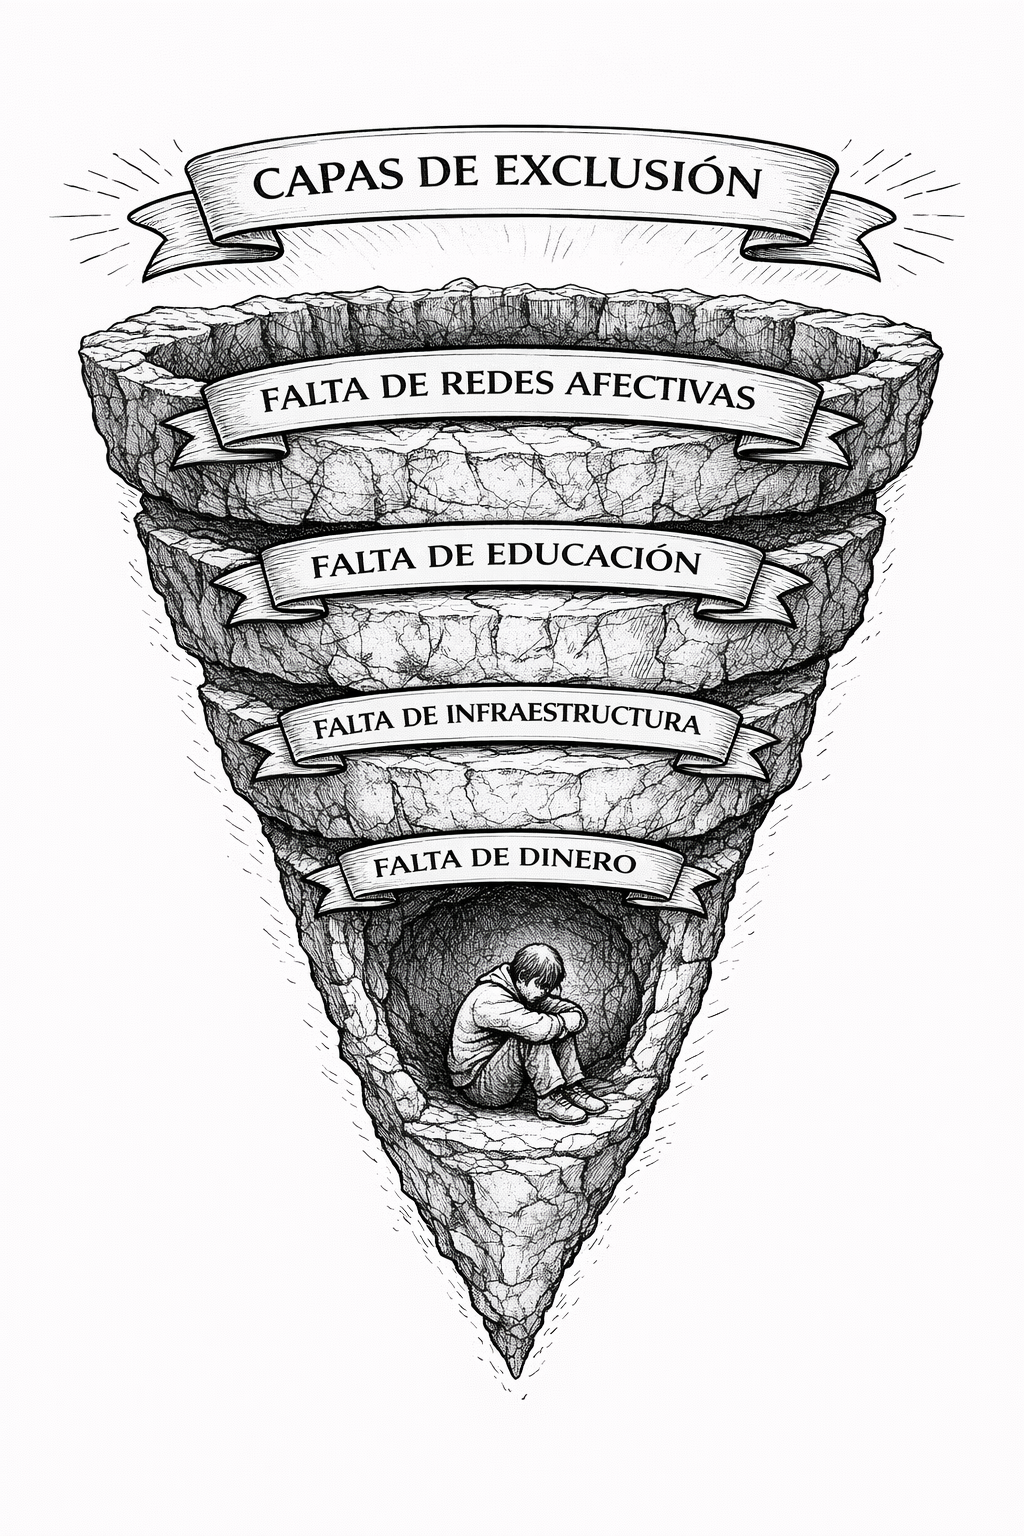
\includegraphics[scale=0.3]{451.png}
		\caption{La pobreza no es solo un tema económico}
	\end{figure}
	
	\momento{Fundamento o criterio de discernimiento}
	
	\marginnote{Cfr. Mayor vulnerabilidad biológica en la pobreza y el estrés crónico (cap. 9)}
	
	La antropología cristiana enseña que el ser humano es un ser sagrado cuya dignidad ontológica permanece intacta aun en situaciones de indigencia social. Sin embargo, la cultura del descarte\index{cultura del descarte|textbf} denunciada por el Papa Francisco actúa como una «mancha de aceite» que invade los territorios más postergados, privando a las personas de su derecho al desarrollo integral. La liberación de las injusticias estructurales es la condición necesaria para que la persona recupere su libertad y su protagonismo.
	
	\momento{Tesis y desarrollo argumental}\\ \\
	La pobreza estructural constituye el escenario de mayor riesgo para el despliegue de las adicciones debido a tres dimensiones críticas:
	\begin{enumerate}
		\item Primero, la privación de recursos básicos, donde la falta de tierra, techo y trabajo digno agota los recursos psíquicos de las familias y genera un estrés crónico que empuja a los jóvenes hacia el consumo como un intento autoterapéutico frente a una realidad intolerable.
		\item Segundo, la invisibilidad y falta de sentido, donde la exclusión social convence al sujeto de que no tiene nada que aportar a la sociedad, sumergiéndolo en un vacío existencial que el narcotráfico aprovecha para ofrecer una falsa pertenencia.
		\item Tercero, la violencia estructural y la desprotección, donde la ausencia del Estado en salud, educación y seguridad permite que el crimen organizado parasite la economía barrial y secuestre los espacios públicos. Ante esto, la inclusión social no es una recompensa por la recuperación, sino la base indispensable para remover los obstáculos que bloquean el despliegue del espíritu.
	\end{enumerate}
	
	\momento{Respuesta a las objeciones} \\
	\begin{enumerate}
		\item Respecto a la primera objeción, si bien el consumo atraviesa todas las clases sociales, la exclusión quita las redes de amparo y las oportunidades de tratamiento, convirtiendo la adicción en una condena de muerte para el pobre.
		\item En cuanto a la segunda objeción, el ejercicio real de la libertad exige condiciones mínimas de justicia; por ello, es deber del Estado garantizar el acceso a derechos humanos fundamentales, mientras que a la comunidad le corresponde brindar el abrazo fraternal que restaure la identidad del hermano como sujeto de derecho y no como objeto de asistencia.
	\end{enumerate}
	
	\subsection{Artículo 2: La feminización de la pobreza como realidad de exclusión múltiple}
	
	\momento{Planteo del tema} \\
	La pobreza estructural no impacta de manera neutral en el tejido social, sino que se ensaña de forma dirigida con las mujeres. Este fenómeno, definido como feminización de la pobreza, crea escenarios de vulnerabilidad extrema donde la falta de acceso a derechos básicos como la tierra, el trabajo digno y la salud empuja a las mujeres a situaciones de supervivencia extrema, como la prostitución o el narcomenudeo.
	
	\momento{Pregunta central} \\
	¿Qué se entiende por feminización de la pobreza y cómo afecta la subjetividad de las mujeres en situación de consumo?
	
	\momento{Posturas u objeciones existentes} \\
	\begin{itemize}
		\item Podría pensarse que la pobreza afecta a hombres y mujeres por igual en los contextos de exclusión y que, por tanto, las carencias materiales son universales para cualquier persona en situación de calle.
		\item Asimismo, suele decirse que resaltar la pobreza femenina es una forma de discriminación hacia los varones, quienes también sufren el flagelo de la adicción en contextos de miseria.
	\end{itemize}
	
	\momento{Fundamento o criterio de discernimiento} \\
	La antropología cristiana reconoce que el pecado social y la injusticia estructural golpean con mayor crueldad a quienes tienen menores posibilidades de defender sus derechos. Reconocer la feminización de la pobreza es un acto de honestidad misionera que permite identificar la «doble condena» que sufren las mujeres: el estigma social por su consumo y el juicio por no cumplir con el rol idealizado de madre perfecta o cuidadora del hogar.
	
	\momento{Tesis y desarrollo argumental}\\ \\
	La feminización de la pobreza es una realidad de exclusión que se manifiesta en tres dimensiones críticas:
	\begin{enumerate}
		\item Primero, la desprotección estatal, donde el sistema no suele ofrecer la misma infraestructura de amparo y rehabilitación a las mujeres que a los varones.
		\item Segundo, la precariedad habitacional y económica, que las expone a mayores riesgos de calleización y violencia, especialmente cuando deben criar solas a sus hijos.
		\item Tercero, la invisibilización de su dolor, donde sus trayectorias de consumo suelen ser silenciadas por la vergüenza social y la presión del entorno familiar. Liberar estas injusticias es la condición previa para que la persona pueda recuperar su dignidad ontológica y su libertad. Para ello, el Estado debe asumir su responsabilidad en la creación de condiciones legislativas y sociales que garanticen el futuro de estas mujeres.
	\end{enumerate}
	
	\momento{Respuesta a las objeciones} \\
	\begin{enumerate}
		\item Respecto a la primera objeción, aunque la pobreza sea general, las mujeres enfrentan barreras de acceso únicas y una exclusión múltiple que las deja en una situación de mayor desamparo biológico y social.
		\item En cuanto a la segunda objeción, señalar esta realidad no resta importancia al dolor del varón, sino que busca una justicia en la respuesta; un modelo de misericordia debe ser sensible a las diferencias para no aplicar una lógica de escritorio que ignore las llagas específicas del cuerpo sufriente de la mujer en el pueblo.
	\end{enumerate}
	
	\subsection{Artículo 3: Los abordajes diferenciados y el acompañamiento específico para mujeres\index{acompañamiento!de mujeres}}
	
	\momento{Planteo del tema} \\
	Dada la complejidad de las trayectorias femeninas en el consumo de sustancias psicoactivas (SPA), resulta insuficiente aplicar protocolos de tratamiento estandarizados. Surge el imperativo de consolidar abordajes diferenciados que contemplen las necesidades específicas de salud mental, seguridad emocional y vínculos familiares propias de la mujer para remover los obstáculos que bloquean su espíritu.
	
	\momento{Pregunta central} \\
	¿Por qué el acompañamiento a mujeres requiere un enfoque metodológico diferenciado y cuáles son los pilares fundamentales para que el proceso sea sostenible?
	
	\momento{Posturas u objeciones existentes} \\
	\begin{itemize}
		\item Podría pensarse que los protocolos de tratamiento deben ser uniformes para garantizar la equidad científica y técnica, considerando que un abordaje específico para mujeres sería un gasto innecesario de recursos o una complicación administrativa.
		\item Asimismo, suele decirse que la atención en centros mixtos es suficiente para abordar cualquier problemática de adicción sin distinción de género.
	\end{itemize}
	
	\momento{Fundamento o criterio de discernimiento}
	
	\marginnote{Cfr. Espiritualidad en la mujer (cap. 7) y Vulnerabilidad de la mujer en el proceso de cambio (cap. 8)}
	
	Un modelo centrado en la persona debe reconocer la radical singularidad de cada historia sagrada. La antropología cristiana enseña que la verdadera equidad no consiste en la igualdad de trato burocrático, sino en la justicia de la respuesta artesanal que se hace cargo de la totalidad de la vida de la persona, adaptando el cuidado a sus heridas particulares.
	
	\momento{Tesis y desarrollo argumental}\\ \\
	El abordaje diferenciado constituye una herramienta de justicia terapéutica fundamentada en cinco dimensiones críticas:
	\begin{enumerate}
		\item Primero, la vulnerabilidad biológica, reconociendo que las mujeres desarrollan consecuencias médicas graves más rápido que los varones (efecto telescopio\marginnote{Cfr. art.~\ref{art:telescopio} (Juzgar, Las sustancias y el Organismo, Diferencias según..., La respuesta fisionógica...)}).
		\item Segundo, la centralidad del trauma, ya que la gran mayoría de las trayectorias femeninas están marcadas por violencias de género y abusos que requieren espacios de seguridad emocional.
		\item Tercero, el acompañamiento ante el abandono familiar, pues a diferencia de los varones, las mujeres suelen enfrentar el proceso en soledad afectiva absoluta.
		\item Cuarto, la protección de la maternidad, eliminando el miedo a que el Estado arrebate la custodia de los hijos como condición para recibir ayuda.
		\item Quinto, el rol del acompañante par, definido como la experta por experiencia que, habiendo transitado y superado el mismo dolor de la adicción o la exclusión, pone su vida al servicio para guiar a otras desde la autoridad que le otorga su propio testimonio de recuperación.
	\end{enumerate}
	
	\momento{Respuesta a las objeciones} \\
	\begin{enumerate}
		\item Respecto a la primera objeción, la especificidad del abordaje no es un lujo técnico, sino la garantía de que el proceso respeto la dignidad inalienable de cada hermana.
		\item En cuanto a la segunda objeción, los centros mixtos a menudo no pueden garantizar el abordaje del trauma complejo ni las necesidades reproductivas de la mujer; por ello, el enfoque diferenciado permite una intervención que no ignore las llagas específicas del cuerpo sufriente de la mujer en el pueblo.
	\end{enumerate}
	
	\subsection{Artículo 4: Los abordajes diferenciados y el acompañamiento específico para varones\index{acompañamiento!de varones}}
	
	\momento{Planteo del tema} 
	El acompañamiento comunitario en los barrios populares se encuentra con una realidad del consumo en los varones que está fuertemente atravesada por lógicas territoriales, dinámicas de calle y mandatos de masculinidad. Con frecuencia, el consumo masculino se vive de manera pública y expresiva, ligado a la cultura de la esquina, la validación entre pares a través del riesgo, la agresión o la inserción en circuitos de criminalidad y violencia. Un abordaje samaritano exige comprender estas especificidades socioculturales para ofrecer herramientas que permitan desarmar estos mandatos y proponer itinerarios de sanación específicos.
	
	\momento{Pregunta central} 
	¿Exige la propuesta del acompañamiento integral la implementación de un abordaje específico que atienda las lógicas territoriales y los mandatos socioculturales de los varones en el centro barrial?
	
	\momento{Posturas u objeciones existentes}
	\begin{itemize}
		\item \submomento{Objeción 1:} Parece que la adicción es una problemática universal y neutra, por lo que el centro barrial debe aplicar los mismos criterios y dinámicas de acompañamiento para todos los sujetos, sin distinción de sus condicionamientos de género o cultura.
		\item \submomento{Objeción 2:} Parece que focalizar en un abordaje específico para varones debilita la vida comunitaria compartida de la parroquia, promoviendo una separación innecesaria dentro de los dispositivos de acogida.
	\end{itemize}
	
	\momento{Fundamento o criterio de discernimiento} 
	Jesús camina con cada uno conociendo su historia y el peso de su cultura. Sanar las heridas de los varones en el barrio exige una mirada encarnada que no ignore los códigos de la calle ni las presiones sociales que sostienen su consumo. El discernimiento pastoral nos urge a brindar un espacio donde el varón pueda deponer las armas de la omnipotencia para reconocer su propia vulnerabilidad y ser abrazado en su dignidad.
	
	\momento{Tesis y desarrollo argumental}\\ 
	El acompañamiento específico para varones dentro del modelo comunitario se despliega bajo los siguientes criterios pastorales y operativos:
	
	\begin{enumerate}
		\item \textbf{Desarmar los mandatos de la masculinidad hegemónica:} En el territorio, el consumo del varón suele estar ligado a la necesidad de demostrar fuerza, aguante o control, ocultando el dolor o la frustración bajo conductas de riesgo. El proceso comunitario debe propiciar espacios seguros donde el varón aprenda a desarmar la exigencia de una masculinidad omnipotente o violenta, permitiéndose expresar el sufrimiento, el miedo y la debilidad sin sentirse juzgado por sus pares.
		
		\item \textbf{La resignificación de la cultura de la esquina y el territorio:} La barra y la esquina funcionan muchas veces como la única red de pertenencia frente a la exclusión. El centro barrial no debe demonizar estos espacios, sino ofrecer una alternativa superadora: transformar la lógica de la banda o el circuito de riesgo en una pertenencia comunitaria positiva, reorientando los códigos de lealtad y fraternidad callejera hacia el servicio común, el cuidado mutuo y el trabajo solidario en el barrio.
		
		\item \textbf{Espacios específicos de palabra y elaboración:} Si bien la riqueza de la PLAPA está en la vida comunitaria común —donde se comparte la mesa, los talleres y la oración—, el abordaje de los varones requiere de instancias específicas (grupos de palabra exclusivos). En estos espacios íntimos de varón a varón se pueden trabajar temáticas complejas como la paternidad ausente o conflictiva, la gestión de la ira, las historias de violencia o encierro, y la reconstrucción de un proyecto de vida responsable y afectivo.
	\end{enumerate}
	
	\momento{Respuesta a las objeciones}
	\begin{itemize}
		\item \submomento{A la primera:} Ignorar que el consumo masculino está moldeado por la cultura de la calle impide desestructurar las causas profundas de sus recaídas y de sus conductas violentas. Un abordaje neutro no logra penetrar la coraza de <<aguante>> con la que el varón se defiende en el barrio; se necesita una clave de lectura relacional y encarnada para que el proceso de reconfiguración de valores sea real.
		\item \submomento{A la segunda:} El espacio específico no aísla al varón de la comunidad, sino que lo prepara para habitarla de una manera más sana. Brindarles un lugar propio para elaborar sus dolores específicos fortalece su inserción en las actividades comunes compartidas, permitiéndoles construir relaciones de verdadero respeto, fraternidad y complementariedad con las mujeres y las familias del centro barrial.
	\end{itemize}
	
	\subsection{Artículo 5: La economía popular y solidaria como motores de identidad y dignidad}
	
	\momento{Planteo del tema} \\
	La recuperación integral de las personas con consumos problemáticos exige superar la visión del trabajo como una simple meta de reintegración económica. Se analiza la necesidad de integrar la dimensión de la economía popular y solidaria como componentes esenciales del proceso terapéutico, capaces de reconstruir hábitos y devolver el sentido de protagonismo social al hermano vulnerabilizado en su propio territorio.
	
	\momento{Pregunta central} \\
	¿Deben integrarse la economía popular y el trabajo digno como elementos esenciales desde las etapas tempranas de la recuperación, o constituyen únicamente objetivos finales de la reintegración social?
	
	\momento{Posturas u objeciones existentes} \\
	\begin{itemize}
		\item Podría pensarse que el trabajo es únicamente un medio de supervivencia económica y que lo relevante es que la persona obtenga ingresos para dejar de ser una carga social.
		\item Asimismo, suele decirse que el empleo debe ser la recompensa final tras haber logrado la abstinencia total, bajo la idea de que la persona aún no posee la disciplina necesaria para cumplir una tarea productiva.
		\item Por otro lado, podría pensarse que el manejo de dinero es un factor de alto riesgo que dispara el deseo de consumo, por lo que debe evitarse durante el tratamiento.
	\end{itemize}
	
	\momento{Fundamento o criterio de discernimiento} \\
	La antropología cristiana y el magisterio del Papa Francisco enseñan que el trabajo es una parte fundamental de la dignidad humana que permite al hombre cultivarse a sí mismo y sostener a su familia. La inclusión económica no es el premio al final del camino, sino una condición de justicia para que la recuperación sea sostenible y digna, permitiendo que el sujeto se reconozca nuevamente como ciudadano con derechos y responsabilidades.
	
	\momento{Tesis y desarrollo argumental}\\ \\
	La integración de la economía popular en la recuperación propone un cambio de paradigma que prioriza el ser sobre el hacer a través de cinco ejes fundamentales:
	\begin{enumerate}
		\item Primero, el trabajo como lazo social, funcionando como un puente para reconstruir el vínculo con la comunidad y transformar al asistido en un sujeto productivo.
		\item Segundo, el fomento del cooperativismo en los sectores populares, impulsando emprendimientos que contemplen la dinámica comunitaria y los tiempos del proceso artesanal.
		\item Tercero, la reeducación financiera, utilizando el dinero de forma pedagógica para transitar hacia una autonomía progresiva y reemplazar la inmediatez de la calle por la planificación.
		\item Cuarto, la misericordia estructurada, que implementa una flexibilidad organizada con reglas claras pero empáticas, entendiendo que el trabajo es un medio para la sanación.
		\item Quinto, la valoración de los talentos propios, donde la inclusión social reconoce las herramientas que los sujetos ya poseen para disputar la economía barrial al narcotráfico.
	\end{enumerate}
	
	\momento{Respuesta a las objeciones} \\
	\begin{enumerate}
		\item Respecto a la primera objeción, el trabajo digno trasciende la supervivencia; es el camino para alcanzar la libertad necesaria para decidir sobre la propia salud y vivienda.
		\item En cuanto a la segunda objeción, el proceso debe ser circular, permitiendo que la persona se pruebe en tareas productivas desde etapas de estabilización para fortalecer su identidad.
		\item Finalmente, frente a la tercera objeción, el riesgo del dinero se mitiga con un control asistido y pedagógico; administrar el primer sueldo de forma acompañada ayuda a ganar seguridad y refuerza la confianza de la familia en el proceso. Para que esto sea posible, el Estado debe asumir su responsabilidad en la creación de políticas públicas que fomenten el empleo y el cooperativismo en los barrios más postergados.
	\end{enumerate}
	
	\subsection{Artículo 6: El abordaje de la movilidad humana y la interculturalidad}
	
	\marginnote{Mt 25, 35\label{mt25.35} — \textit{Fui forastero y me hospedaste}}
	
	\momento{Planteo del tema} \\
	La movilidad humana\index{acompañamiento!de migrantes} y la interculturalidad no son fenómenos externos al territorio, sino dimensiones que modifican profundamente el tejido social donde se realiza la acción comunitaria. Se analiza la necesidad de integrar la realidad del hermano migrante como una clave de lectura esencial para el acompañamiento integral de los consumos problemáticos, reconociendo que el desarraigo y la falta de red suelen potenciar la vulnerabilidad social.
	
	\momento{Pregunta central} \\
	¿De qué manera debe el manual integrar la movilidad humana y la interculturalidad como dimensiones fundamentales del acompañamiento pastoral?
	
	\momento{Posturas u objeciones existentes} \\
	\begin{itemize}
		\item Podría pensarse que la migración es un tema estrictamente político o sociológico que no debería ocupar un lugar central en un manual de adicciones, el cual debe focalizarse únicamente en la salud mental y la recuperación de sustancias psicoactivas.
		\item Se argumenta a menudo que los procesos de acompañamiento deben ser estandarizados para todos los habitantes de un territorio sin distinguir el origen cultural, bajo la premisa de que la adicción afectaría la biología humana por igual, independientemente del trasfondo histórico de la persona.
	\end{itemize}
	
	\momento{Fundamento o criterio de discernimiento} \\
	El Papa Francisco enseña que la movilidad humana es un signo de los tiempos que requiere una pastoral específica que respete las culturas y la riqueza espiritual de cada pueblo. La antropología cristiana afirma que todo migrante posee una dignidad inalienable; por tanto, la Iglesia debe actuar como un «hospital de campaña» que acoja la orfandad y la vulnerabilidad extrema que el proceso migratorio suele generar, reconociendo que no hay sanación sin enraizamiento.
	
	\momento{Tesis y desarrollo argumental}\\ \\
	El abordaje de la movilidad humana se fundamenta en cinco dimensiones críticas para la justicia social:
	\begin{enumerate}
		\item Reconocimiento de la dignidad ontológica: Se debe denunciar la práctica social de considerar a los migrantes como sujetos de segunda clase, lo cual agrava su invisibilidad y el riesgo de recurrir al consumo como escape frente al desprecio.
		\item Impacto en la configuración territorial: La migración transforma los barrios; la comunidad organizada debe introducirse en estas nuevas realidades para integrar a los migrantes en sus círculos de cuidado, evitando que el aislamiento los empuje hacia las redes del narcotráfico.
		\item Respuesta educativa y de nivelación: Es imperativo proponer estrategias de refuerzo pedagógico para niños y adolescentes migrantes que han visto interrumpida su escolaridad, ofreciéndoles espacios promocionales que generen pertenencia.
		\item Acompañamiento en el encierro: Se reconoce que los migrantes privados de libertad enfrentan una soledad mayor por la falta de red biográfica; por ello, el acompañamiento debe ser diferenciado para evitar que el desarraigo derive en una reincidencia en el consumo.
		\item Inculturación de la pastoral: La espiritualidad propuesta debe adaptar su lenguaje para que el hermano migrante descubra a un Dios que camina con él en su propia historia, transformando el dolor del viaje en un proceso de resurrección comunitaria.
	\end{enumerate}
	
	\momento{Respuesta a las objeciones} \\
	\begin{enumerate}
		\item Respecto a la primera objeción, aunque la migración tenga aristas políticas, su raíz es humana; la vulnerabilidad que genera la falta de tierra, techo y trabajo es un condicionante directo del consumo que la misión evangelizadora no puede ignorar.
		\item En cuanto a la segunda, aunque la adicción tenga una base biológica, la recuperación es un proceso vincular; ignorar la cultura del otro es una forma de fragmentación administrativa que impide generar el vínculo de confianza necesario para que la persona se sienta amada en su totalidad.
	\end{enumerate}
	
	\newpage
	
	\section{El Acompañante y la Incidencia Política}
	
	Esta sección define el rol del acompañante no solo como un apoyo afectivo, sino como un sujeto de incidencia política capaz de transformar las estructuras de exclusión. Inspirado en la caridad política\index{caridad política} propuesta por el Papa Francisco, se invita a la Iglesia a pasar de la respuesta pastoral concreta a la exigencia de políticas públicas humanizantes que garanticen los derechos de los más vulnerables. El texto enfatiza que, si bien el Estado es el garante de derechos, este no tiene la capacidad de generar comunidad por sí solo, por lo que resulta imperativo defender el saber territorial y el principio de subsidiariedad para fortalecer las redes de cuidado sin que sean absorbidas por la burocracia estatal. Finalmente, se reivindica una mirada profética que denuncie el pecado social y las estructuras de injusticia, posicionando a los acompañantes pares como actores protagónicos en la disputa de sentido frente a modelos que priorizan la sanitización o la represión del espacio público.
	
	
	
	\subsection{Artículo 1: El ejercicio de la caridad política como misión eclesial}
	
	\marginnote{Mi 6, 8\label{mi6.8} — \textit{¿Qué pide de ti el Señor? Practicar la justicia, amar la misericordia, caminar humildemente con tu Dios}}
	
	\momento{Planteo del tema} \\
	La misión evangelizadora frente a los consumos problemáticos no agota su sentido en la asistencia inmediata. Se analiza la necesidad de que la Iglesia asuma el ejercicio de la caridad política\index{caridad política|textbf}, transitando de la ayuda individual a la transformación de las estructuras sociales que generan exclusión y desamparo.
	
	\momento{Pregunta central} \\
	¿Debe la Iglesia introducirse en la caridad política como parte de su misión en el abordaje de las adicciones?
	
	\momento{Posturas u objeciones existentes} \\
	\begin{itemize}
		\item Podría pensarse que la Iglesia debe limitar su acción exclusivamente a la esfera espiritual y religiosa, evitando introducirse en asuntos de políticas públicas para no desvirtuar su misión y convertirse en una organización no gubernamental (ONG) de asistencia social.
		\item Se argumenta que la responsabilidad del cuidado y la recuperación es competencia exclusiva del Estado. Bajo esta visión, la Iglesia debería simplemente rellenar los huecos donde la asistencia pública no llega, sin cuestionar ni incidir en las estructuras de poder.
		\item Podría pensarse que en territorios dominados por la narcocultura y la violencia, el ejercicio de la caridad política es peligroso e inútil, debido a la posible complicidad de las estructuras estatales con el crimen organizado.
	\end{itemize}
	
	\momento{Fundamento o criterio de discernimiento} \\
	El Papa Francisco enseña que la caridad es el corazón del espíritu de la política y se manifiesta como un amor preferencial por los últimos. La antropología cristiana afirma que la fe es inseparable de la defensa de la dignidad humana; por tanto, cuando la comunidad se une para generar procesos de fraternidad y justicia, está ejerciendo una forma de caridad que trasciende lo individual para volverse social.
	
	\momento{Tesis y desarrollo argumental}\\ \\
	La Iglesia ejerce la caridad política\index{caridad política!ejes estratégicos} como una manifestación irrenunciable de su propia esencia a través de cinco ejes estratégicos:
	\begin{enumerate}
		\item \textbf{Denuncia profética}: Consiste\index{voz profética|textbf} en desmitificar la narcopolítica y denunciar las políticas «sanitizantes» que pretenden limpiar el espacio público tratando a las personas en consumo como desechos o delincuentes, en lugar de reconocer su dignidad sagrada.
		\item \textbf{Incidencia en el Estado como garante}: Exigir que el Estado asuma sus obligaciones constitucionales en salud, identidad y vivienda. La Iglesia actúa como el hilo que articula estas respuestas fragmentadas para que lleguen efectivamente al territorio.
		\item \textbf{Alianza para el bien común}: Promover una articulación entre la universidad (investigación), el sector empresarial (empleo) y la comunidad organizada (presencia territorial) para construir políticas públicas basadas en la realidad y no en el escritorio.
		\item \textbf{Reocupación de los espacios democráticos}: Animar a la comunidad a habitar nuevamente los clubes, mutuales y centros barriales como antídoto contra el individualismo que el narcotráfico aprovecha para ocupar el territorio.
		\item \textbf{Defensa del derecho al cuidado}: Promover el derecho autónomo e ineludible a cuidar, ser cuidado\index{cuidado!derecho al} y al autocuidado, especialmente para las poblaciones que los sistemas penal o sanitario han invisibilizado.
	\end{enumerate}
	
	\momento{Respuesta a las objeciones} \\
	\begin{enumerate}
		\item Respecto a la primera objeción, la Iglesia no es una ONG, pero su compromiso social es la encarnación de la misericordia de Cristo, que se hace cargo de la integridad del hombre en todas sus dimensiones.
		\item En cuanto a la segunda, aunque el Estado tiene la responsabilidad primaria, este no tiene la capacidad de generar por sí solo vínculos de pertenencia; la Iglesia aporta el saber territorial y la experiencia de familia que la rigidez administrativa no puede ofrecer.
		\item Frente a la tercera, precisamente donde impera la cultura de la muerte es donde la comunidad organizada debe entrar para dignificar la vida. La caridad política permite transformar el miedo en organización y ofrecer un relato de esperanza frente a la dictadura del narcotráfico.
	\end{enumerate}
	
	\textbf{Conclusión} \\
	El ejercicio de la caridad política\index{caridad política!dimensión profética} permite que la Iglesia sea una voz profética\index{voz profética} en el espacio público, transformando las condiciones de injusticia en escenarios de libertad y protagonismo para los hermanos más vulnerabilizados.
	
	\subsection{Artículo 2: La importancia fundamental del autocuidado para el agente pastoral}
	
	\marginnote{Mc 6, 31\label{mc6.31} — \textit{Vengan ustedes solos a un lugar apartado, para descansar un poco}}
	
	\momento{Planteo del tema} \\
	El servicio pastoral en el ámbito de las adicciones implica un contacto constante con el dolor, la violencia y realidades humanas complejas que suponen un alto costo emocional. Se analiza si la estrategia del autocuidado\index{acompañamiento!autocuidado del agente}\index{autocuidado} es un componente opcional o una condición indispensable para asegurar la salud integral del agente y la calidad del acompañamiento.
	
	\momento{Pregunta central} \\
	¿Es fundamental la estrategia del autocuidado para garantizar la eficacia y continuidad de la labor del agente pastoral en el ámbito de las adicciones?
	
	\momento{Posturas u objeciones existentes} \\
	\begin{itemize}
		\item Podría pensarse que el agente pastoral debe entregarse totalmente al servicio sin reservas, siguiendo el ejemplo del sacrificio de Cristo, y que preocuparse por el propio bienestar personal constituye un acto de egoísmo o una falta de celo apostólico ante la urgencia del sufrimiento ajeno.
		\item Se dice a menudo que el apoyo espiritual y la gracia de Dios son suficientes para sostener al cuidador. Bajo esta visión, no se requerirían estrategias técnicas de autocuidado o pausas humanas, ya que la misión misma proporcionaría la fuerza necesaria para no desfallecer.
	\end{itemize}
	
	\momento{Fundamento o criterio de discernimiento} 
	
	\marginnote{Cfr. art. 8.7.4 (autocuidado clínico)}
	
	El descanso no es opcional, sino una necesidad ordenada por el propio Cristo para quienes están en el centro del servicio. La Iglesia, como hospital de campaña, debe cuidar a sus propios soldados heridos por la fatiga y el dolor, reconociendo que el Espíritu Santo actúa también a través de las mediaciones humanas y el respeto por los límites biológicos.
	
	\momento{Tesis y desarrollo argumental}\\ \\
	El autocuidado\index{autocuidado|textbf} constituye un principio ético y una necesidad teológica para la sostenibilidad del servicio, fundamentada en cinco dimensiones:
	\begin{enumerate}
		\item \textbf{Garantía de la calidad del cuidado}: El estado psicofísico del agente condiciona significativamente la ayuda que brinda; un cuidador agotado pierde la capacidad de escucha activa y empatía, convirtiendo la misión en una estructura rígida y defensiva.
		\item \textbf{Prevención del agotamiento (burnout)}: El\index{burnout|textbf} acompañamiento permanente en contextos de vulnerabilidad puede derivar en fatiga por compasión. El autocuidado protege la salud mental del agente frente al impacto del trauma secundario.
		\item \textbf{Sostenibilidad de la misión}: El agotamiento crónico impide la continuidad del servicio. Gestionar la propia vida y las propias emociones es una condición para que el servicio pastoral sea duradero y no una respuesta espasmódica.
		\item \textbf{Reconocimiento de la vulnerabilidad humana}: El agente pastoral no es un superhéroe, sino una persona vulnerable que también necesita ternura y cuidado. El pastor debe dejarse cuidar y reconocer que la periferia donde trabaja es también un espejo de sus propias carencias.
		\item \textbf{Teología del descanso}: Siguiendo el magisterio del Papa Francisco, el descanso es parte integrante de la misión y un derecho que glorifica a Dios. Saber sentarse en el «banco de suplentes» permite que otros tomen la posta y evita la tentación de la omnipotencia.
	\end{enumerate}
	
	\momento{Respuesta a las objeciones} \\
	\begin{enumerate}
		\item Respecto a la primera objeción, la caridad bien entendida empieza por la propia persona; no se puede transmitir el amor de Dios si el corazón del agente está seco por la fatiga. El autocuidado\index{autocuidado!y caridad} permite que el servicio sea una expresión de solidaridad y no una carga desgastante.
		\item En cuanto a la segunda, aunque la fe sea el motor, el ser humano es una unidad de cuerpo y alma. La formación técnica y el apoyo de grupos de pares son mediaciones humanas necesarias para que la gracia de Dios fructifique en una vida equilibrada.
	\end{enumerate}
	
	\textbf{Conclusión} \\
	El autocuidado garantiza que el agente pastoral permanecerá como un instrumento dócil y saludable de la misericordia divina, asegurando que el acompañamiento sea siempre un encuentro humano de sanación y no una rutina burocrática agotadora.
	
	\subsection{Artículo 3: El mandato de primerear y callejear en las periferias del consumo}
	
	\marginnote{Lc 14, 21-23\label{lc14.21} — \textit{Sal en seguida por las plazas y las calles de la ciudad, y trae aquí a los pobres, a los lisiados, a los ciegos y a los cojos}}
	
	\momento{Planteo del tema} \\
	La identidad de una comunidad que acompaña consumos problemáticos se define por su movimiento hacia afuera. Se analiza el significado profundo de los mandatos de «primerear»\index{primerear} y «callejear»\index{callejeadas} como gestos que rompen con la autorreferencialidad eclesial para buscar la vida herida en sus escenarios cotidianos.
	
	\momento{Pregunta central} \\
	¿Qué implica para la Iglesia el mandato de primerear y callejear dentro de las periferias humanas del consumo y la exclusión?
	
	\momento{Posturas u objeciones existentes} \\
	\begin{itemize}
		\item Podría pensarse que la Iglesia debe esperar en sus templos a que las personas busquen ayuda por voluntad propia, y que salir de forma insistente a buscarlas podría interpretarse como una invasión de la privacidad o una falta de respeto a la libertad individual.
		\item Podría pensarse que callejear y mancharse con la realidad de la calle pone en riesgo la santidad y la imagen institucional, sugiriendo que la comunidad debe mantenerse centrada en sus ritos para ser un faro de moralidad inalterable.
	\end{itemize}
	
	\begin{figure}[h!]
		\centering
		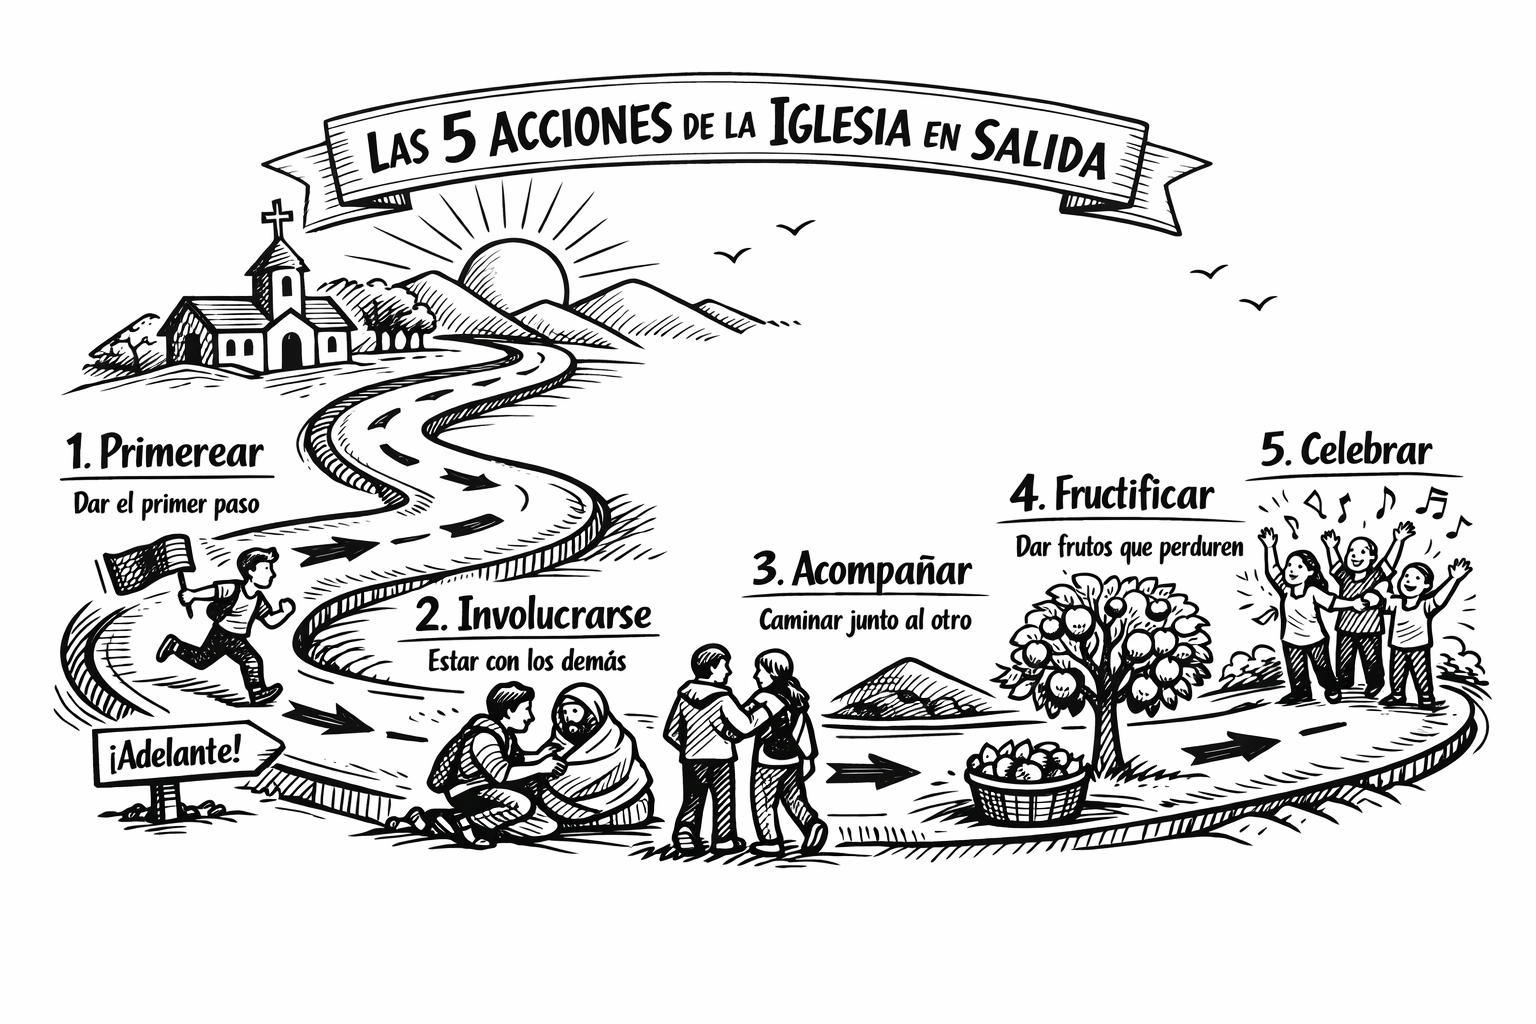
\includegraphics[scale=0.25]{46.png}
		\caption{El método de la Iglesia en salida}
	\end{figure}
	
	\momento{Fundamento o criterio de discernimiento} \\
	El Papa Francisco afirma que prefiere una Iglesia accidentada, herida y manchada por salir a la calle, antes que una Iglesia enferma por el encierro y la comodidad de sus propias seguridades. La comunidad evangelizadora debe tomar la iniciativa, introducirse en los procesos humanos y acompañar la vida por más dura que sea, reconociendo que Dios siempre nos primerea\index{primerear!fundamento teológico} en el amor.
	
	\momento{Tesis y desarrollo argumental}\\ \\
	Los conceptos de primerear y callejear definen una actitud pastoral que transforma la presencia territorial en cuatro dimensiones:
	\begin{enumerate}
		\item \textbf{Primerear (Tomar la iniciativa)}: Significa\index{primerear|textbf} no esperar a que el excluido llegue, sino adelantarse y salir al encuentro de los que están lejos. Es la respuesta de quien se siente amado primero por Dios y desea llevar ese bálsamo a los cruces de los caminos.
		\item \textbf{Callejear}: Es\index{callejeadas|textbf} la disposición activa de buscar la vida que sufre en los rincones más ocultos, como esquinas, plazas y puentes. Implica introducirse en la vida cotidiana de los demás para acortar distancias, asumiendo la realidad del otro hasta tener «olor a oveja».
		\item \textbf{Habitar la periferia}: No se trata de un recorrido superficial, sino de detener el paso para mirar a los ojos y escuchar al que quedó al costado del camino. La Iglesia se reconoce como un «hospital de campaña» que cura heridas urgentes antes de preguntar por tecnicismos.
		\item \textbf{Tocar la carne de Cristo}: Implica renunciar a los cobertizos de seguridad para entrar en contacto directo con la miseria y el dolor del hermano. Al hacerlo, la vida se complica maravillosamente y la comunidad vive la verdadera experiencia de ser pueblo.
	\end{enumerate}
	
	\momento{Respuesta a las objeciones} \\
	\begin{enumerate}
		\item Respecto a la primera objeción, primerear no es invadir, sino ofrecer una misericordia inagotable a quienes se sienten invisibles para la sociedad. Es un gesto de projimidad\index{projimidad} que busca devolver la esperanza a quienes la cultura del abandono ha empujado a dejar de mirar el futuro.
		\item En cuanto a la segunda, la santidad de la Iglesia no se protege en el aislamiento, sino que se nutre en el servicio. La verdadera mundanidad espiritual es la que se disfraza de prácticas religiosas vacías mientras ignora el clamor de los hermanos más rotos.
	\end{enumerate}
	
	\textbf{Conclusión} \\
	Primerear y callejear son las acciones que permiten a la Iglesia ser fiel a su misión, transformando el desprecio social en un encuentro de dignidad donde cada persona es reconocida como un ser sagrado.
	
	
	
	\chapter{El Espíritu Humano}
	
	La dimensión espiritual es el constitutivo esencial del ser humano que nos impulsa a preguntarnos para qué estamos en este mundo y qué vida queremos elegir para nosotros y para los demás. Lejos de ser un anexo religioso o un sentimiento subjetivo, el espíritu es la esencia del ser donde reside nuestra identidad más honda, así como nuestra relación, otorgándonos una dignidad absoluta e inalienable que ninguna caída puede borrar.
	
	Al juzgar la problemática del consumo de sustancias psicoactivas (SPA) desde la fe, reconocemos que el trastorno por uso de sustancias provoca una desconexión progresiva con esta realidad interior, convirtiéndose a menudo en una «búsqueda espiritual fallida» que intenta anestesiar heridas profundas de orfandad y llenar una «grieta existencial» que solo el encuentro con la trascendencia puede colmar.
	
	Por ello, este manual nos invita a mirar a la persona como una unidad integral de cuerpo y alma, rescatando al corazón como el centro unificador e íntimo donde la razón y el sentimiento se integran y donde reside la identidad más profunda. Es en este núcleo de la personalidad donde se fraguan las exigencias de felicidad, verdad y justicia que el consumo de SPA no logra saciar, abriendo paso a un proceso de reconexión y sanación profunda guiado por el Espíritu.
	
	Este capítulo está compuesto por 9 secciones:
	
	\begin{enumerate}
		\item Naturaleza, definición y fundamentos
		\item La condición espiritual
		\item La adicción como un fenómeno espiritual
		\item El proceso de reconexión
		\item El camino cristiano
		\item Los sacramentos
		\item La sabiduría espiritual
		\item La espiritualidad en la mujer
		\item El ancla de la comunidad	
	\end{enumerate}
	
	
	\section{Naturaleza, definición y fundamentos}
	
	Esta sección establece que la espiritualidad es el constitutivo esencial de la identidad humana y la fuerza motora que orienta a la persona hacia el significado de su existencia. Se fundamenta en la dignidad ontológica infinita de ser creados a imagen de Dios, una marca indeleble que el consumo de sustancias psicoactivas no puede borrar ni eliminar. Al reconocer que el ser humano es constitutivamente una búsqueda de sentido, la comunidad se organiza para despertar esta dimensión latente.
	
	\subsection{Artículo 1: La espiritualidad como constitutivo esencial y fuerza motora de la identidad}
	
	\marginnote{Gn 2, 7\label{gen2.7} — \textit{Sopló en su nariz un aliento de vida, y el hombre se convirtió en un ser viviente}}
	
	\momento{Planteo del tema}\\
	Al abordar el consumo de sustancias, es común centrarse en los daños biológicos o sociales. Sin embargo, surge la necesidad de discernir si lo espiritual es una respuesta accidental ante el malestar o si constituye el núcleo mismo del ser humano. Debemos juzgar si las preguntas fundamentales sobre el sentido de la vida representan la fuerza motora que integra la afectividad y la razón en el corazón de la persona.
	
	\momento{Pregunta central}\\
	¿De qué manera la dimensión espiritual define la identidad humana y actúa como la fuerza que mueve al sujeto hacia la búsqueda de significado?
	
	\momento{Posturas u objeciones existentes}
	\begin{itemize}
		\item \submomento{Objeción 1:} La neurociencia demuestra que el consumo altera los circuitos de recompensa; por tanto, la motivación es puramente química y no espiritual.
		\item \submomento{Objeción 2:} Muchos sujetos solo buscan a Dios cuando han «tocado fondo», sugiriendo que la espiritualidad es un efecto del dolor y no una esencia previa.
		\item \submomento{Objeción 3:} Si una persona no profesa una fe religiosa, parecería carecer de esta fuerza motora, invalidando la espiritualidad como constitutivo universal.
	\end{itemize}
	
	\begin{figure}[h!]
		\centering
		\includegraphics[scale=0.25]{211.png}
		\caption{Espiritualidad e identidad}
	\end{figure}
	
	\momento{Fundamento o criterio de discernimiento}\\
	Se establece que la esencia y existencia del hombre están constitutivamente relacionadas con Dios. El ser humano es «capaz de Dios» y posee una dignidad absoluta que reside en su identidad más honda. El corazón se reconoce como el centro unificador donde se integran la razón y el sentimiento, siendo el núcleo donde se fraguan las exigencias de felicidad y verdad.
	
	\momento{Tesis y desarrollo argumental}\\
	Respondemos que la espiritualidad es el eje motor de la identidad humana por las siguientes razones:
	\begin{itemize}
		\item \textbf{Unidad antropológica operativa:} El espíritu es el principio integrador que permite al sujeto examinar su propia biología y tomar decisiones sobre su historia. La espiritualidad faculta a la persona para no solo sobrevivir, sino ser protagonista de su vida mediante el testimonio.
		\item \textbf{Diferencia entre potencia y condición:} Es vital distinguir entre la potencia espiritual (esencia inalienable) y la condición espiritual (estado dinámico de la relación con Dios). El consumo no crea la necesidad espiritual, sino que es una búsqueda fallida ante una grieta existencial previa.
		\item \textbf{Dinamicidad del espíritu:} La espiritualidad permite al ser humano tomar distancia de su realidad inmediata. Esta capacidad de trascendencia es la que habilita la reconexión y el compromiso con la vida.
	\end{itemize}
	
	\momento{Respuesta a las objeciones}
	\begin{itemize}
		\item \submomento{A la primera:} La espiritualidad utiliza la neuroplasticidad\marginnote{Cfr. art.~\ref{art:neuroplasticidad} (Juzgar, Brevísimo Glosario)} asistida por la gracia para reorientar la voluntad. El propósito vital actúa como un estímulo superior capaz de reorganizar los circuitos de recompensa que la sustancia había secuestrado.
		\item \submomento{A la segunda:} El malestar actúa como una «alarma existencial» que revela la grieta espiritual previa. El dolor no crea la espiritualidad, sino que es la señal de que el sistema de trascendencia reclama su lugar tras la anestesia del consumo.
		\item \submomento{A la tercera:} Se debe distinguir entre espiritualidad universal y religión institucional. Todo ser humano ejerce su fuerza espiritual al elegir qué orientación le da a su vida y al buscar la verdad en sus vínculos mediante el diálogo fraterno.
	\end{itemize}
	
	\subsection{Artículo 2: La dimensión espiritual como búsqueda del sentido y propósito vital}
	
	\momento{Planteo del tema}\\
	Dada la naturaleza multifactorial del trastorno por uso de sustancias, surge la necesidad de preguntarnos por el sentido de la existencia. Esta búsqueda constituye el eje sobre el cual se construye la identidad y la libertad del ser humano para decidir sobre su propia vida y su relación con los demás.
	
	\momento{Pregunta central}\\
	¿Cómo se define la dimensión espiritual como la búsqueda del propósito y el lugar que cada uno ocupa en el mundo?
	
	\momento{Posturas u objeciones existentes}
	\begin{itemize}
		\item \submomento{Objeción 1:} Las preguntas sobre el proyecto de vida pertenecen al campo de la psicología o la ética y no necesariamente a una dimensión espiritual trascendente.
		\item \submomento{Objeción 2:} En personas con consumos severos, estas preguntas pierden relevancia ante la urgencia de la supervivencia inmediata o la satisfacción del deseo.
	\end{itemize}
	
	\momento{Fundamento o criterio de discernimiento}\\
	Se afirma que la espiritualidad es la esencia del ser que mueve a una persona a buscar significado. Si no se desarrolla esta dimensión, la totalidad de la persona queda vedada, convirtiéndose en fuente de angustia existencial. La búsqueda de sentido permanece latente incluso en los cuadros más graves.
	
	\momento{Tesis y desarrollo argumental}\\
	Respondemos que la dimensión espiritual se define por estas preguntas porque ellas constituyen el «para qué» de la existencia:
	\begin{itemize}
		\item \textbf{Finalidad del ser:} Lo espiritual aborda la tarea de interrogarse por la razón de ser. Es el espacio donde el sujeto decide qué orientación le da a su vida mediante la escucha activa de su propio deseo de plenitud.
		\item \textbf{Sutura de la grieta existencial:} La adicción suele instalarse donde las preguntas no tienen respuesta. La recuperación auténtica implica una reconexión con el propósito vital que la sustancia intentó suplantar.
	\end{itemize}
	
	\momento{Respuesta a las objeciones}
	\begin{itemize}
		\item \submomento{A la primera:} Mientras la psicología gestiona la operatividad de los procesos psíquicos, la espiritualidad otorga la dirección última y el fin absoluto. El espíritu es el que pregunta por el significado que la psique sola no puede responder.
		\item \submomento{A la segunda:} El consumo compulsivo es la «forma física» de una pregunta espiritual desesperada. El deseo de eternizar el efecto de la sustancia es la manifestación distorsionada de una sed de infinito que solo la reconexión con el sentido puede saciar.
	\end{itemize}
	
	\subsection{Artículo 3: El fundamento de la dignidad ontológica inalienable en la imagen de Dios}
	
	\marginnote{Gn 1, 26-27\label{gen1.26} — \textit{Hagamos al ser humano a nuestra imagen, según nuestra semejanza... lo creó a imagen de Dios}}
	
	\momento{Planteo del tema}\\
	En el acompañamiento, encontramos a menudo hermanos cuya vida parece haber perdido rastro de humanidad. El estigma suele reducir a la persona a categorías de «descarte». Es imperativo discernir si la dignidad es una construcción moral que puede perderse o si es un dato previo e incólume que permanece bajo la noche de la adicción.
	
	\momento{Pregunta central}\\
	¿De qué manera el ser creado a imagen de Dios fundamenta una dignidad que no puede ser eliminada por el pecado ni por las situaciones de consumo?
	
	\momento{Posturas u objeciones existentes}
	\begin{itemize}
		\item \submomento{Objeción 1:} La dignidad se asocia con el ejercicio de la razón. Una persona con deterioro cognitivo grave parece perder aquello que la hace específicamente humana.
		\item \submomento{Objeción 2:} El pecado y las acciones que dañan a la comunidad degradan al hombre, haciéndole perder su valor ante Dios.
	\end{itemize}
	
	\begin{figure}[h!]
		\centering
		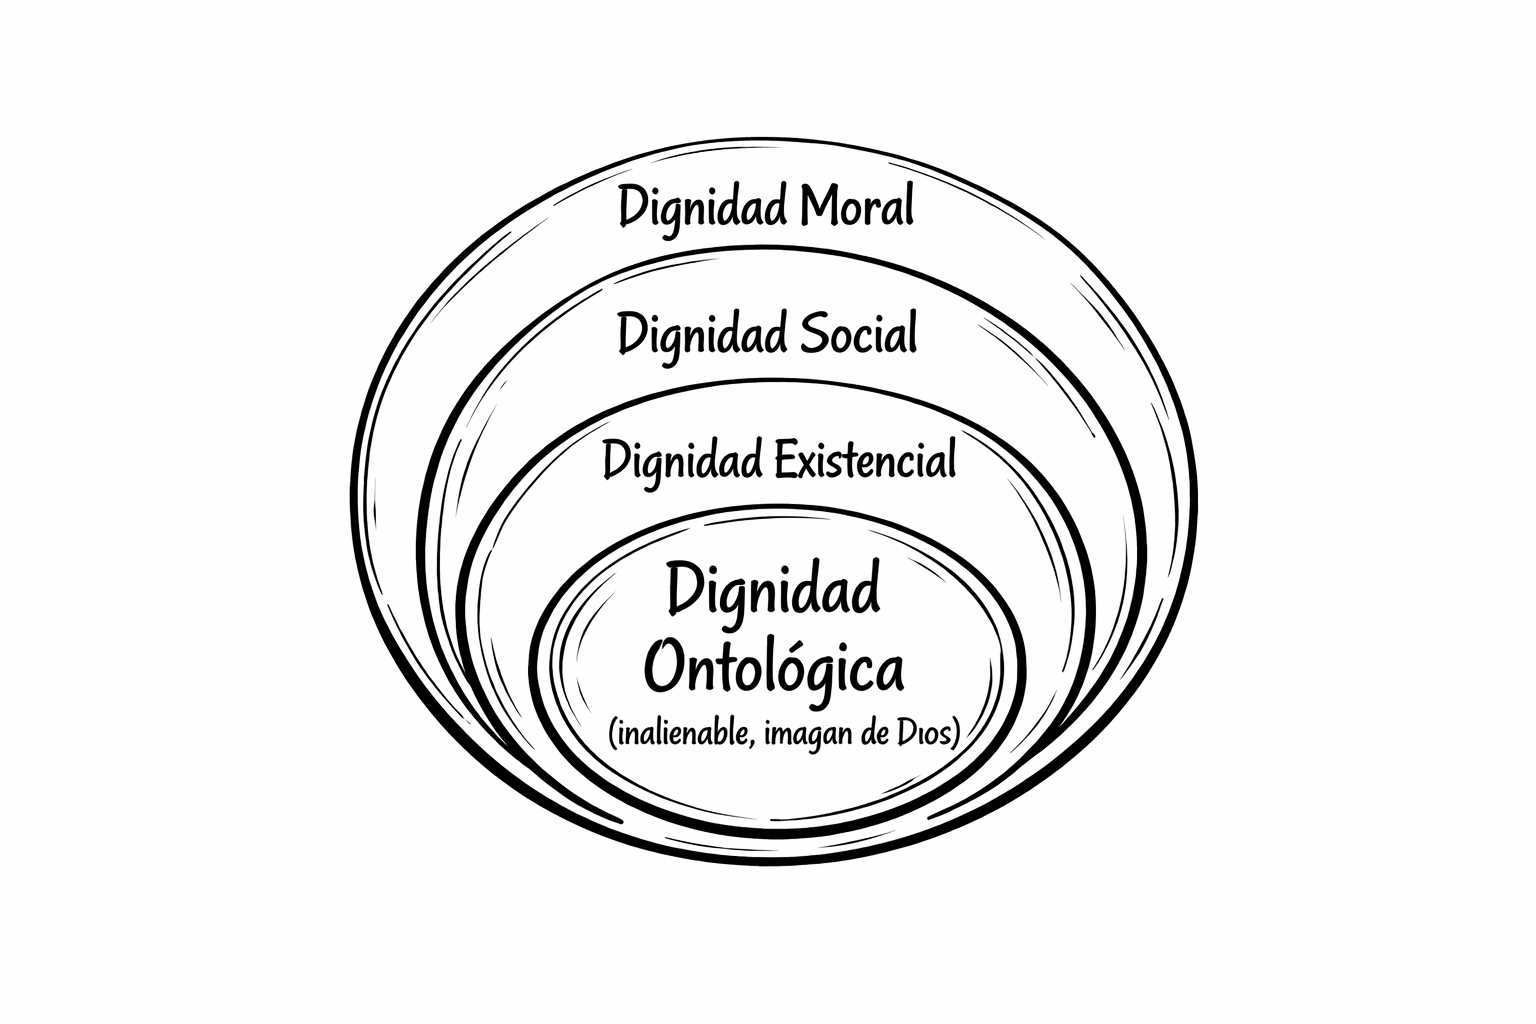
\includegraphics[scale=0.25]{213.png}
		\caption{La dignidad, según \textit{Dignitas Infinita}}
	\end{figure}
	
	\momento{Fundamento o criterio de discernimiento}\\
	Se establece que una dignidad infinita\index{dignidad|textbf} corresponde a cada persona más allá de toda circunstancia. Se introduce la cuádruple distinción: dignidad ontológica (vinculada al ser), moral (ejercicio de la libertad), social (condiciones de vida) y existencial (paz y esperanza). La dignidad ontológica es inalienable.
	
	\momento{Tesis y desarrollo argumental}\\
	Respondemos que la dignidad ontológica es la garantía primordial de la salud integral\index{dignidad!como garantía de salud integral}:
	\begin{itemize}
		\item \textbf{Primacía del ser sobre el acto:} El sujeto subsiste con toda su dignidad incluso si no puede ejercer sus capacidades. El juicio pastoral distingue entre el «acto indigno» y la «persona digna».
		\item \textbf{Redención como confirmación:} La dignidad se revela plenamente en Cristo, quien asume la existencia humana confirmando el valor inestimable de quienes el mundo califica como indignos.
	\end{itemize}
	
	\momento{Respuesta a las objeciones}
	\begin{itemize}
		\item \submomento{A la primera:} La dignidad no es un desempeño funcional de la razón, sino un atributo intrínseco del ser. Así como el sol existe aunque las nubes lo tapen, la marca divina en el hermano permanece intacta bajo el oscurecimiento provocado por la sustancia.
		\item \submomento{A la segunda:} La libertad contra el amor puede herir la semejanza divina, pero nunca borrar el hecho originario de ser criatura querida. Esta raíz indestructible es la que permite iniciar cualquier diálogo fraterno de restauración.
	\end{itemize}
	
	
	\subsection[Artículo 4: Espiritualidad y religión]{Artículo 4: La distinción necesaria entre espiritualidad y religión}
	
	
	\momento{Planteo del tema}\\
	Surge el desafío de abordar la dimensión espiritual de personas que no necesariamente profesan una fe. Es imperativo clarificar si la espiritualidad es un patrimonio exclusivo de los creyentes o si es una capacidad universal que impulsa a todo sujeto a interrogarse por su razón de ser.
	
	\momento{Pregunta central}\\
	¿Es necesario distinguir entre espiritualidad y religión para garantizar un proceso de reconexión inclusivo y respetuoso?
	
	\momento{Posturas u objeciones existentes}
	\begin{itemize}
		\item \submomento{Objeción 1:} Dado que la adicción es una enfermedad espiritual y Dios es quien sana, la espiritualidad sería intrínsecamente un fenómeno religioso.
		\item \submomento{Objeción 2:} Desvincular ambos conceptos podría parecer un intento de diluir el mensaje del Evangelio y de Jesucristo.
	\end{itemize}
	
	\momento{Fundamento o criterio de discernimiento}\\
	Se afirma que esta dimensión fundante no debe confundirse con la creencia en una divinidad concreta. La espiritualidad no es un privilegio de los religiosos; todo ser humano debe elegir qué vida llevar. El corazón es el centro donde reside la identidad más profunda.
	
	\momento{Tesis y desarrollo argumental}\\
	Respondemos que es indispensable distinguir ambos planos para una pastoral eficaz:
	\begin{itemize}
		\item \textbf{Universalidad frente a Institucionalidad:} La espiritualidad es la búsqueda del «para qué» de la existencia (potencia). La religión propone un lenguaje y un camino concreto para vivir esa relación (condición).
		\item \textbf{Respeto a la libertad:} Reconocer la espiritualidad universal evita excluir a quienes no buscan ayuda en sistemas tradicionales, permitiendo un encuentro basado en la realidad del otro.
		\item \textbf{Distinción sin separación:} Si bien la distinción entre espiritualidad y religión es analíticamente necesaria para acompañar a toda persona sin condiciones previas, no debe interpretarse como una separación que valide una espiritualidad autorreferencial o desvinculada de la comunidad. Desde la perspectiva cristiana que anima este manual, la búsqueda espiritual auténtica no se agota en la interioridad del sujeto: tiende constitutivamente al encuentro con los demás y, en última instancia, a la mediación comunitaria y sacramental donde esa búsqueda encuentra su plenitud. El hermano que llega sin fe no es excluido por eso; pero el horizonte del acompañamiento incluye la posibilidad de que su búsqueda de sentido lo conduzca, en libertad y a su ritmo, hacia el encuentro con Cristo y con la comunidad eclesial. La espiritualidad universal es la puerta; la vida comunitaria y sacramental es la casa a la que esa puerta puede abrirse.
	\end{itemize}
	
	\momento{Respuesta a las objeciones}
	\begin{itemize}
		\item \submomento{A la primera:} La sanación espiritual comienza por recuperar la conciencia de la propia dignidad, lo cual es previo a cualquier práctica religiosa formal.
		\item \submomento{A la segunda:} La distinción no diluye el anuncio de Jesucristo sino que lo fortalece al encarnarlo en la realidad concreta del hermano. Reconocer la espiritualidad universal como punto de partida permite que el primer anuncio no sea una imposición sino una propuesta que respeta el tiempo y la historia del otro. El agente pastoral sabe que la sed de sentido que habita en todo ser humano es, como enseña la tradición cristiana, una sed de Dios que aún no se reconoce como tal. Distinguir espiritualidad de religión no es renunciar a proponer el Evangelio; es discernir el momento y el modo de hacerlo para que la propuesta sea recibida como lo que es: una buena noticia y no una condición de acceso al cuidado.
	\end{itemize}
	
	\subsection{Artículo 5: La distinción entre la vida psíquica y la apertura a lo divino}
	
	\momento{Planteo del tema}\\
	En el acompañamiento suele haber una confusión que reduce lo no biológico a una sola categoría psíquica o espiritual. Es vital recuperar una distinción funcional que permita entender cómo el ser humano posee dimensiones que se ven afectadas de modo diverso por el trastorno por uso de sustancias.
	
	\momento{Pregunta central}\\
	¿De qué manera la distinción entre psique y espíritu permite comprender la unidad integral de la persona sin caer en una dualidad del alma?
	
	\momento{Posturas u objeciones existentes}
	\begin{itemize}
		\item \submomento{Objeción 1:} En muchos enfoques terapéuticos se utiliza «psique» y «espíritu» como sinónimos, por lo que no habría necesidad de distinguirlos.
		\item \submomento{Objeción 2:} Si el consumo altera los mecanismos biológicos del cerebro, tanto la voluntad como la trascendencia serían simples subproductos de la química cerebral.
	\end{itemize}
	
	\momento{Fundamento o criterio de discernimiento}\\
	La Iglesia enseña que el hombre es un ser entero: espíritu, alma y cuerpo. «Espíritu» significa que el hombre está ordenado a un fin sobrenatural. Aunque sostenemos la unidad inseparable, la antropología tripartita es una herramienta valiosa para diferenciar la afectividad (alma) de la trascendencia (espíritu).
	
	\momento{Tesis y desarrollo argumental}\\
	Respondemos que es útil reconocer una tricotomía de dimensiones en la unidad de la persona:
	\begin{itemize}
		\item \textbf{El lugar de las emociones y la trascendencia:} Esta distinción permite identificar que en el trastorno por uso de sustancias, mientras la psique sufre la impulsividad, el espíritu conserva la potencia de buscar significado.
		\item \textbf{El espíritu como apertura:} El espíritu es el centro más profundo del alma que la abre a la gracia. Permite tomar distancia de los impulsos emocionales para elegir un bien superior mediante el testimonio.
	\end{itemize}
	
	\momento{Respuesta a las objeciones}
	\begin{itemize}
		\item \submomento{A la primera:} Mientras la psicología trata los procesos afectivos y conductuales (psique), la espiritualidad se ocupa de la vocación existencial y la relación con el Absoluto (espíritu).
		\item \submomento{A la segunda:} La ciencia explica la maquinaria biológica, pero reducir todo a lo biológico ignora la capacidad radical de ser protagonista de la propia historia. Lo que sucede en el cuerpo tiene un correlato en el espíritu y viceversa.
	\end{itemize}
	
	\newpage
	
	\section{La condición espiritual}
	
	Esta sección analiza la condición espiritual como el estado dinámico de la relación que el ser humano establece con Dios y con los demás, partiendo siempre de su historia personal de afectividad, sus vínculos y su ética. Se explora cómo los entornos de desprotección o de orfandad afectiva dañan esta condición, sumiendo al sujeto en una grieta existencial. Al mismo tiempo, se propone al corazón como el centro unificador donde la libertad del sujeto puede ser restaurada mediante el encuentro comunitario y el despertar de su potencia espiritual innata.
	
	\subsection{Artículo 1: La condición espiritual y el desarrollo de la potencia a través de los vínculos}
	
	\momento{Planteo del tema}\\
	En la pastoral de acompañamiento, observamos que las trayectorias de consumo suelen nacer de historias de orfandad y vínculos rotos. Surge la necesidad de discernir si el espíritu humano puede desarrollarse como una fuerza puramente autónoma o si requiere de la mediación de otros para mantenerse sano. Debemos juzgar si las heridas de la afectividad definen la tierra en la que la relación con Dios debe germinar o si son elementos accidentales que no condicionan la salud del alma.
	
	\momento{Pregunta central}\\
	¿En qué medida la salud de la condición espiritual depende de la historia vincular y de la mediación de la comunidad?
	
	\momento{Posturas u objeciones existentes}
	\begin{itemize}
		\item \submomento{Objeción 1:} Dado que la relación con Dios es constitutiva del ser, la salud espiritual debería ser independiente de las contingencias de los vínculos humanos.
		\item \submomento{Objeción 2:} Si la espiritualidad dependiera de los vínculos, aquellos que han sufrido abandono perderían su capacidad de trascendencia, lo cual contradice la inalienabilidad del espíritu.
		\item \submomento{Objeción 3:} La potencia espiritual debería poder activarse desde la pura interioridad del sujeto sin necesidad de mediaciones externas que podrían resultar fallidas.
	\end{itemize}
	
	\begin{figure}[h!]
		\centering
		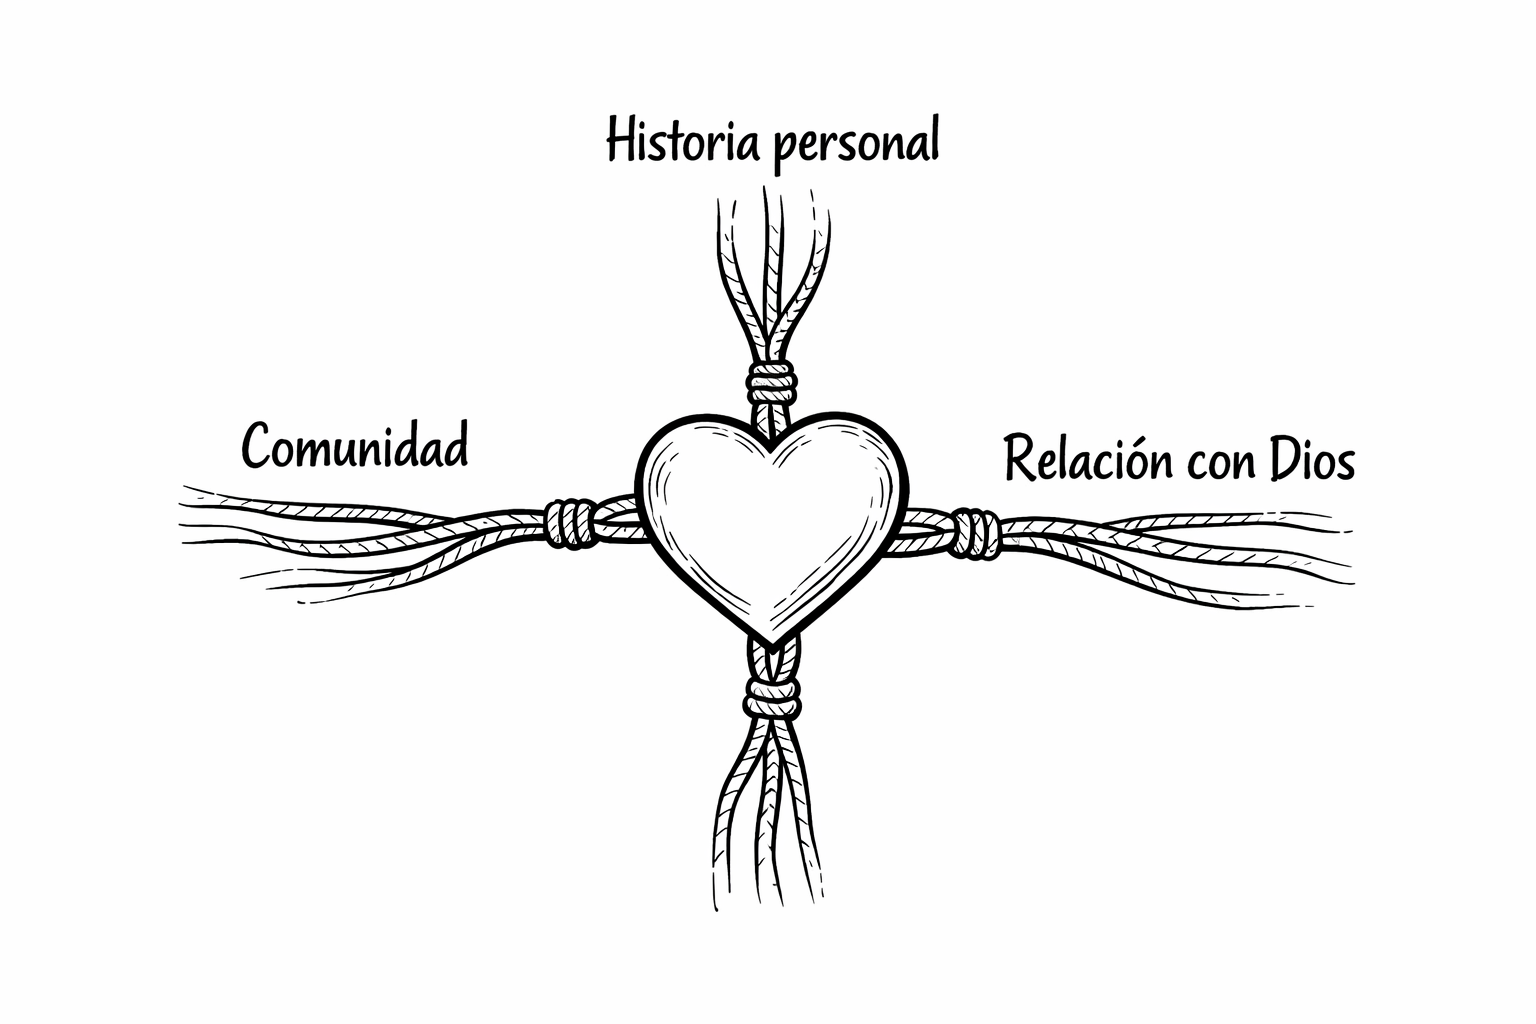
\includegraphics[scale=0.25]{221.png}
		\caption{Espiritualidad y vínculos}
	\end{figure}
	
	\momento{Fundamento o criterio de discernimiento}\\
	Se establece que no existe espiritualidad sin los otros. El ser humano es constitutivamente relacional y los demás funcionan como espejos necesarios para plantear la propia respuesta al mundo. El amor se reconoce como el medicamento que permite la restauración del ser cuando los vínculos primarios\index{vínculo!y vínculos primarios} han sido dañados, despertando la dimensión espiritual mediante la projimidad y el testimonio.
	
	\momento{Tesis y desarrollo argumental}\\
	Respondemos que la vivencia saludable de la espiritualidad está ligada al tejido vincular por las siguientes razones:
	\begin{itemize}
		\item \textbf{La espiritualidad como semilla:} El desarrollo humano es potencial. Aunque la información para la trascendencia es innata, requiere de vínculos generativos para desplegarse. Si el entorno es hostil, la dimensión espiritual queda herida, generando la grieta existencial donde se instala el trastorno por uso de sustancias.
		\item \textbf{Necesidad de mediación humana:} El corazón es el centro donde se procesan los vínculos. Sin confianza primaria, el yo no logra sustentarse para abrirse a la trascendencia. La comunidad repara mediante el afecto lo que la orfandad fracturó.
		\item \textbf{Sutura de la fractura interna:} La salud espiritual se manifiesta en la capacidad de amar. Al ofrecer un entorno de escucha activa, la comunidad permite que el flujo natural de la vida espiritual vuelva a fluir, removiendo los obstáculos del trauma.
	\end{itemize}
	
	\momento{Respuesta a las objeciones}
	\begin{itemize}
		\item \submomento{A la primera:} El espíritu humano no opera en el vacío, sino encarnado en la relación. Así como el cerebro necesita estímulos para desarrollarse, la potencia espiritual requiere de los vínculos para ser reconocida y valorada por el propio sujeto como una realidad operativa en su vida.
		\item \submomento{A la segunda:} La orfandad no elimina la esencia, pero sí daña la condición o el estado de salud del espíritu. El sujeto sigue siendo digno, pero su capacidad de experimentar esa dignidad se ve bloqueada por redes de memoria desadaptativas que solo el diálogo fraterno puede desarmar.
		\item \submomento{A la tercera:} La mediación comunitaria no crea la espiritualidad, sino que actúa como el entorno facilitador que remueve los obstáculos afectivos. El encuentro con el hermano es el signo sensible que permite al sujeto creer en un Dios que antes le resultaba ajeno por el desamparo acumulado.
	\end{itemize}
	
	\subsection{Artículo 2: El impacto de la orfandad y la falta de amor de hogar en el desarrollo espiritual}
	
	\marginnote{Jn 14, 18\label{jn14.18} — \textit{No los dejaré huérfanos; volveré a ustedes}}
	
	\momento{Planteo del tema}\\
	Al analizar las trayectorias de consumo, se observa que el inicio suele estar precedido por una sensación de invisibilidad familiar y social. Resulta imperativo juzgar si la carencia de un fundamento sólido de amor en el hogar hiere de manera profunda la capacidad del sujeto para conectar con su propia trascendencia o si el espíritu permanece inmune a la desprotección del entorno.
	
	\momento{Pregunta central}\\
	¿Cómo afecta al desarrollo de la condición espiritual el haber crecido en un entorno de orfandad y sin redes de contención?
	
	\momento{Posturas u objeciones existentes}
	\begin{itemize}
		\item \submomento{Objeción 1:} El libre albedrío permite que el sujeto elija su camino espiritual independientemente de su historia vincular previa.
		\item \submomento{Objeción 2:} La orfandad puede funcionar como un motor de resiliencia que impulse al sujeto a buscar a Dios con más fuerza al no tener apoyos humanos.
	\end{itemize}
	
	\begin{figure}[h!]
		\centering
		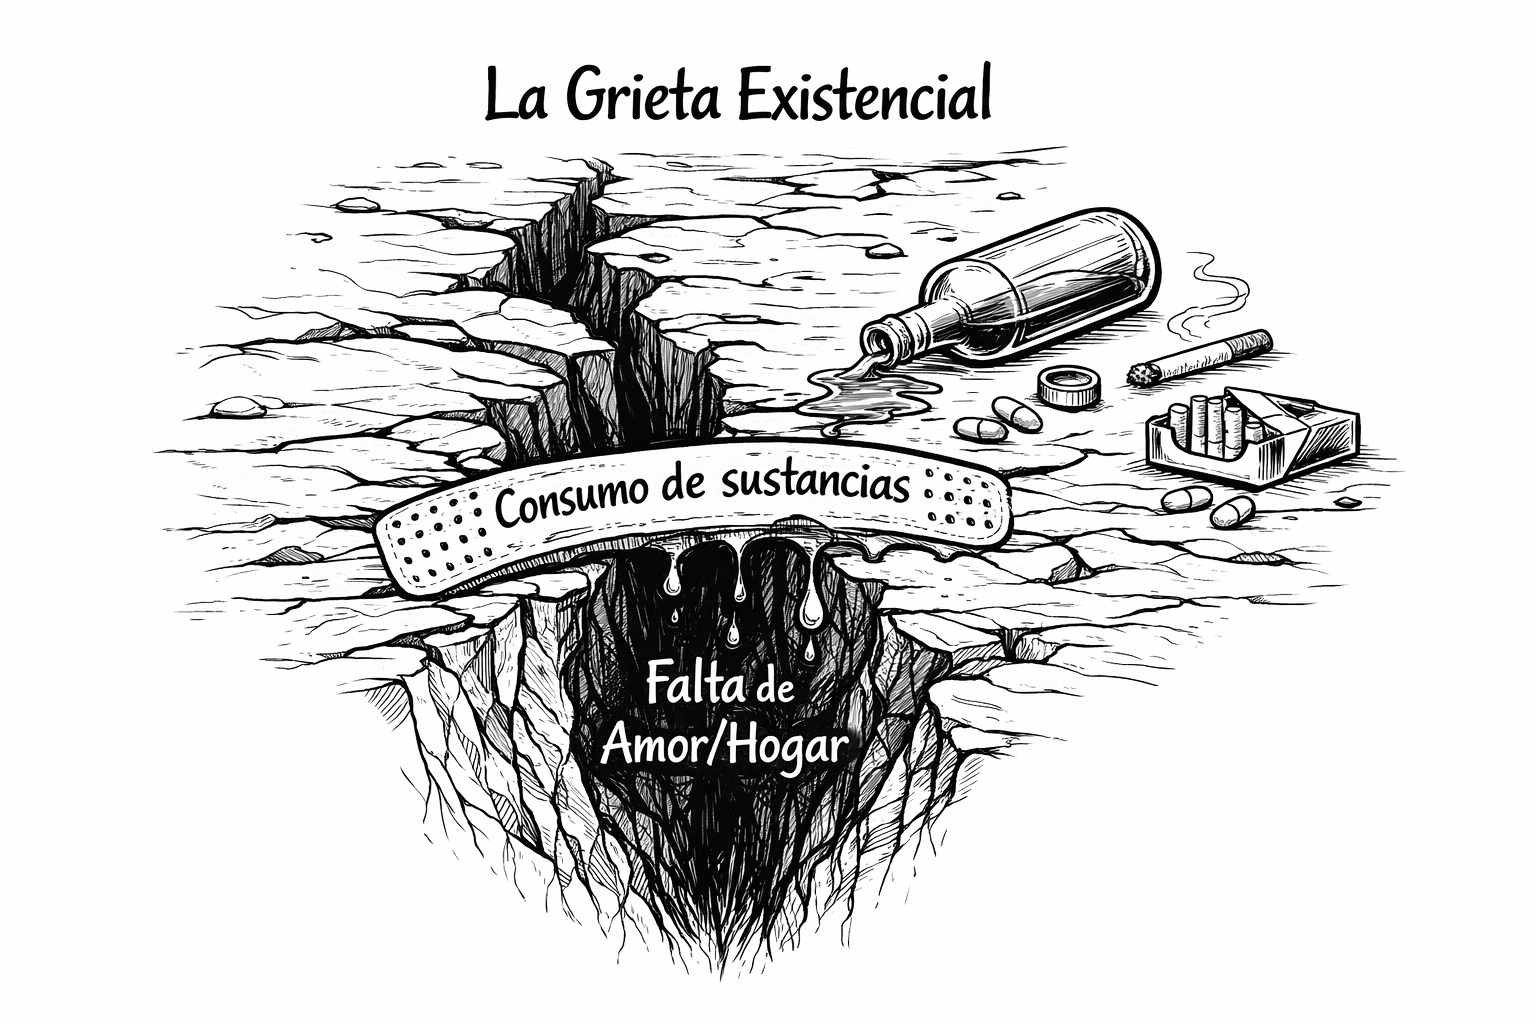
\includegraphics[scale=0.25]{222.png}
		\caption{Orfandad y adicción}
	\end{figure}
	
	\momento{Fundamento o criterio de discernimiento}\\
	Se afirma que la orfandad produce una desvinculación con el horizonte de vida. Si no se desarrolla la dimensión espiritual por falta de contención, algo de la totalidad de la persona queda vedado. La Iglesia enseña que el amor es el medicamento que permite la restauración del ser frente a la desolación de la cultura del descarte.
	
	\momento{Tesis y desarrollo argumental}\\
	Respondemos que el entorno de orfandad afecta gravemente la condición espiritual del sujeto mediante estos puntos:
	\begin{itemize}
		\item \textbf{Fractura del sentido de pertenencia:} Quien no encuentra la mesa compartida busca amparo en el consumo, que intenta llenar falsamente el vacío. Esta falta de raíces dificulta responder para quién vale la pena gastar la vida.
		\item \textbf{Obstrucción de la identidad:} Al no sentirse amado por referentes humanos, al sujeto le resulta difícil reconocerse como imagen de Dios, pues el espejo humano donde debía verse reflejado estaba roto por el descuido o el maltrato.
	\end{itemize}
	
	\momento{Respuesta a las objeciones}
	\begin{itemize}
		\item \submomento{A la primera:} La libertad requiere condiciones de seguridad para ejercerse plenamente. En contextos de abandono, el consumo aparece como una estrategia de supervivencia ante un mundo insoportable y no como una elección libre y soberana de la voluntad.
		\item \submomento{A la segunda:} Si bien Dios actúa en la oscuridad, la sanación requiere que una comunidad asuma el rol de la familia ausente. La resiliencia no es un acto solitario, sino el fruto de ser mirado con amor por otros a través de la escucha activa.
	\end{itemize}
	
	\subsection{Artículo 3: El lugar del corazón en la estructura del espíritu humano}
	
	\momento{Planteo del tema}\\
	No basta con definir al espíritu como una capacidad abstracta; es necesario identificar el lugar antropológico donde el ser humano procesa su existencia e integra sus facultades. En la tradición bíblica y en el magisterio reciente, este lugar es el corazón, el núcleo de la personalidad donde la razón y el sentimiento convergen. Comprender cómo este centro unificador es herido es clave para entender la desvitalización que caracteriza al trastorno por uso de sustancias.
	
	\momento{Pregunta central}\\
	¿Cómo se integra el corazón como el centro de la razón y el sentimiento donde residen las exigencias de plenitud?
	
	\momento{Posturas u objeciones existentes}
	\begin{itemize}
		\item \submomento{Objeción 1:} La neurociencia sitúa la toma de decisiones en la corteza prefrontal\marginnote{Cfr. art.~\ref{art:cortex} (Juzgar, Las sustancias y el organismo, Definición..., Riesgos...)}, dejando al corazón como una mera metáfora literaria sin base en el funcionamiento humano real.
		\item \submomento{Objeción 2:} En una persona con un consumo severo, las exigencias de verdad parecen haber desaparecido, siendo reemplazadas por la impulsividad biológica.
	\end{itemize}
	
	\momento{Fundamento o criterio de discernimiento}\\
	El corazón es el centro unificador de la persona, allí donde cada uno hace su síntesis y donde se encuentra la fuente de sus elecciones. El ser humano es una unidad integral con un centro que otorga orientación a la vida y donde reside la capacidad de ser capaz de Dios.
	
	\momento{Tesis y desarrollo argumental}\\
	Respondemos que el corazón constituye el centro de la estructura del espíritu:
	\begin{itemize}
		\item \textbf{Sede de las exigencias originales:} El corazón es un impulso hacia el infinito. Estas exigencias actúan como la brújula del espíritu que permite evaluar si la vida tiene sentido o es una existencia sin rumbo.
		\item \textbf{Punto de unión entre inteligencia y afecto:} Es donde el sujeto siente la verdad y razona sus afectos, permitiendo una mirada integral que supera la fragmentación a través del diálogo fraterno.
	\end{itemize}
	
	\momento{Respuesta a las objeciones}
	\begin{itemize}
		\item \submomento{A la primera:} Aunque se localicen funciones en áreas cerebrales, el corazón representa el centro de gravedad existencial. La fe comprende los procesos cognitivos como la actividad de un espíritu encarnado que integra la totalidad del ser, algo que la descripción de las neuronas por sí sola no puede agotar.
		\item \submomento{A la segunda:} Las exigencias de felicidad no mueren, sino que son anestesiadas. El proceso de recuperación ayuda al hermano a volver a escuchar su propio corazón mediante la escucha activa, desplazando progresivamente la voz de la compulsión química.
	\end{itemize}
	
	\subsection{Artículo 4: El papel de la libertad en la relación con Dios}
	
	\marginnote{Gal 5, 1\label{gal5.1} — \textit{Para la libertad nos liberó Cristo. Manténganse, pues, firmes y no se sometan otra vez al yugo de la esclavitud}}
	
	\momento{Planteo del tema}\\
	Surge una tensión entre la dignidad de la persona y la realidad de la adicción, descrita a menudo como una esclavitud química. Resulta imperativo discernir si el hermano conserva la capacidad radical de elegir a Dios en medio de su dependencia o si la libertad es una mera ilusión ante la fuerza de las sustancias psicoactivas.
	
	\momento{Pregunta central}\\
	¿Qué papel juega la libertad en la capacidad del sujeto para abrirse a la relación con Dios en un contexto de consumo problemático?
	
	\momento{Posturas u objeciones existentes}
	\begin{itemize}
		\item \submomento{Objeción 1:} El consumo compulsivo altera la capacidad de juicio de tal manera que la persona pierde el dominio real sobre sus actos, quedando su libertad anulada por la fisiología.
		\item \submomento{Objeción 2:} La pobreza estructural condiciona la vida de tal manera que las personas dejan de tener posibilidades reales de elegir, borrando cualquier búsqueda trascendente.
	\end{itemize}
	
	\momento{Fundamento o criterio de discernimiento}
	
	\marginnote{Cfr. La paradoja de la voluntad cautiva (cap. 9, dimensión biológica)}
	
	Dios ha creado al hombre dotándolo del dominio de sus actos. Aunque la libertad esté frecuentemente oscurecida por condicionamientos sociales o químicos, nunca es destruida en su raíz última. La relación con Dios es constitutiva y jamás puede ser eliminada de la estructura esencial del ser.
	
	\momento{Tesis y desarrollo argumental}\\
	Respondemos que la libertad es el postulado que permite al hombre responder al amor divino:
	\begin{itemize}
		\item \textbf{Libertad que necesita ser liberada:} En el trastorno por uso de sustancias la libertad está debilitada pero no muerta. El encuentro con la gracia ofrece una fuerza que la voluntad sola no posee para superar la grieta existencial.
		\item \textbf{El protagonismo del sujeto:} La reconexión no es una imposición, sino un acto voluntario donde el sujeto decide poner su vida al cuidado de un poder superior, recuperando el timón de su existencia mediante el testimonio.
	\end{itemize}
	
	\momento{Respuesta a las objeciones}
	\begin{itemize}
		\item \submomento{A la primera:} El espíritu conserva la capacidad radical de pedir ayuda, que es el primer acto de libertad recuperada. El tratamiento integral utiliza la neuroplasticidad\marginnote{Cfr. art.~\ref{art:neuroplasticidad} (Juzgar, Brevísimo Glosario)} asistida por la gracia para formar nuevos vínculos que fortalecen la voluntad frente al impulso.
		\item \submomento{A la segunda:} Las condiciones sociales afectan el ejercicio de la libertad, pero no anulan la capacidad de optar por la esperanza. Incluso en la miseria, el ser humano es un sujeto activo capaz de iniciar un diálogo fraterno que transforme su realidad interna y externa.
	\end{itemize}
	
	\newpage
	
	\section{La adicción como un fenómeno espiritual}
	
	Esta sección reconoce que el trastorno por uso de sustancias funciona a menudo como un intento autoterapéutico de anestesiar una existencia que se ha vuelto intolerable debido al trauma y la falta de un horizonte de sentido. El consumo se instala en una fractura de la identidad profunda, provocando una desconexión progresiva del sujeto con su esencia y con la trascendencia. La adicción se manifiesta como un camino errado que busca llenar con gratificación inmediata un vacío de pertenencia que solo puede ser colmado mediante el encuentro con el amor divino en comunidad.
	
	\subsection{Artículo 1: La naturaleza del consumo problemático como fractura de la trascendencia}
	
	\momento{Planteo del tema}\\
	Históricamente, se ha juzgado el consumo como un «vicio» o una «debilidad de carácter», visión que suele derivar en estigma y culpa. Sin embargo, la experiencia revela que el consumo de sustancias toca las fibras más profundas de la identidad. Resulta imperativo discernir si estamos ante un simple error de la voluntad o ante una crisis del espíritu que clama por una respuesta al sentido último de la vida.
	
	\momento{Pregunta central}\\
	¿De qué manera debe juzgarse el consumo problemático: como una falta moral o como una fractura en la conexión con la trascendencia?
	
	\momento{Posturas u objeciones existentes}
	\begin{itemize}
		\item \submomento{Objeción 1:} El uso de sustancias fuera de prescripción constituye una falta grave que sitúa el problema estrictamente en el terreno de la moralidad y el pecado.
		\item \submomento{Objeción 2:} Dado que el inicio del consumo nace de una decisión voluntaria, el sujeto es el único responsable de su trayectoria, lo que refuerza la idea de una degradación moral por elección.
	\end{itemize}
	
	\momento{Fundamento o criterio de discernimiento}\\
	Se establece que detrás de cualquier dependencia hay un vacío de significado. La Iglesia, al actuar como refugio, sostiene que la dignidad del hermano permanece intacta incluso cuando su capacidad de actuar libremente se encuentra nublada. El juicio pastoral prioriza la integridad de la persona, reconociendo que el trastorno es un síntoma de una fractura espiritual previa.
	
	\momento{Tesis y desarrollo argumental}\\
	Respondemos que el trastorno por uso de sustancias, además de sus dimensiones biológicas y psicológicas analizadas en los capítulos correspondientes, involucra una fractura de la trascendencia que constituye su herida más profunda y menos visible. Esta dimensión espiritual no sustituye las otras sino que las atraviesa: el vacío de sentido no opera en paralelo al daño neurobiológico ni al trauma psíquico, sino que los habita desde dentro, configurando el suelo existencial sobre el cual esos daños se instalan y se sostienen. Por las siguientes razones:
	\begin{itemize}
		\item \textbf{Anestesia del desamparo:} El consumo funciona como un intento de ocultar heridas de abuso que el sujeto no puede procesar. No es una búsqueda de maldad, sino un escape de una realidad percibida como una amenaza constante.
		\item \textbf{Falso absoluto:} La sustancia aparece como una promesa de bienestar inmediato que busca sustituir la verdadera trascendencia. El «instante mágico» del consumo intenta llenar el espacio que corresponde a la relación con Dios y con los hermanos.
	\end{itemize}
	
	\momento{Respuesta a las objeciones}
	\begin{itemize}
		\item \submomento{A la primera:} Aunque existan actos desordenados, el enfoque debe priorizar la sanación de la herida espiritual. La falta moral es secundaria a la desolación interior; tratar al hermano con misericordia es lo que permite iniciar un diálogo fraterno restaurador.
		\item \submomento{A la segunda:} Si bien el inicio puede ser operativo, la progresión hacia la dependencia despoja al sujeto de su autonomía real. El juicio debe centrarse en la pérdida de libertad provocada por la esclavitud química, ofreciendo un acompañamiento que humanice el recorrido a través del testimonio.
	\end{itemize}
	
	\subsection{Artículo 2: La adicción como búsqueda espiritual fallida e intento anestésico de reparación}
	
	\marginnote{Jr 2, 13\label{jr2.13} — \textit{Mi pueblo ha cometido un doble pecado: me abandonaron a mí, manantial de aguas vivas, para cavarse cisternas, cisternas agrietadas que no retienen el agua}}
	
	\momento{Planteo del tema}\\
	Detrás de cada adicción reside una desolación profunda. Surge la necesidad de discernir si el consumo compulsivo es, en su raíz, un intento desesperado de la persona por reconectarse con lo trascendente a través de un medio equivocado que, en lugar de liberar, termina por anestesiar la identidad y fracturar los vínculos.
	
	\momento{Pregunta central}\\
	¿Es posible comprender la adicción como una búsqueda espiritual fallida y un intento autoterapéutico de reparar heridas de la afectividad?
	
	\momento{Posturas u objeciones existentes}
	\begin{itemize}
		\item \submomento{Objeción 1:} La neurociencia define la adicción como una afección de los circuitos de recompensa; por tanto, es un proceso fisiológico y no una búsqueda de significado.
		\item \submomento{Objeción 2:} Atribuir el consumo a una «autoterapia» espiritual podría debilitar la responsabilidad individual frente al daño cometido a la comunidad.
	\end{itemize}
	
	\begin{figure}[h!]
		\centering
		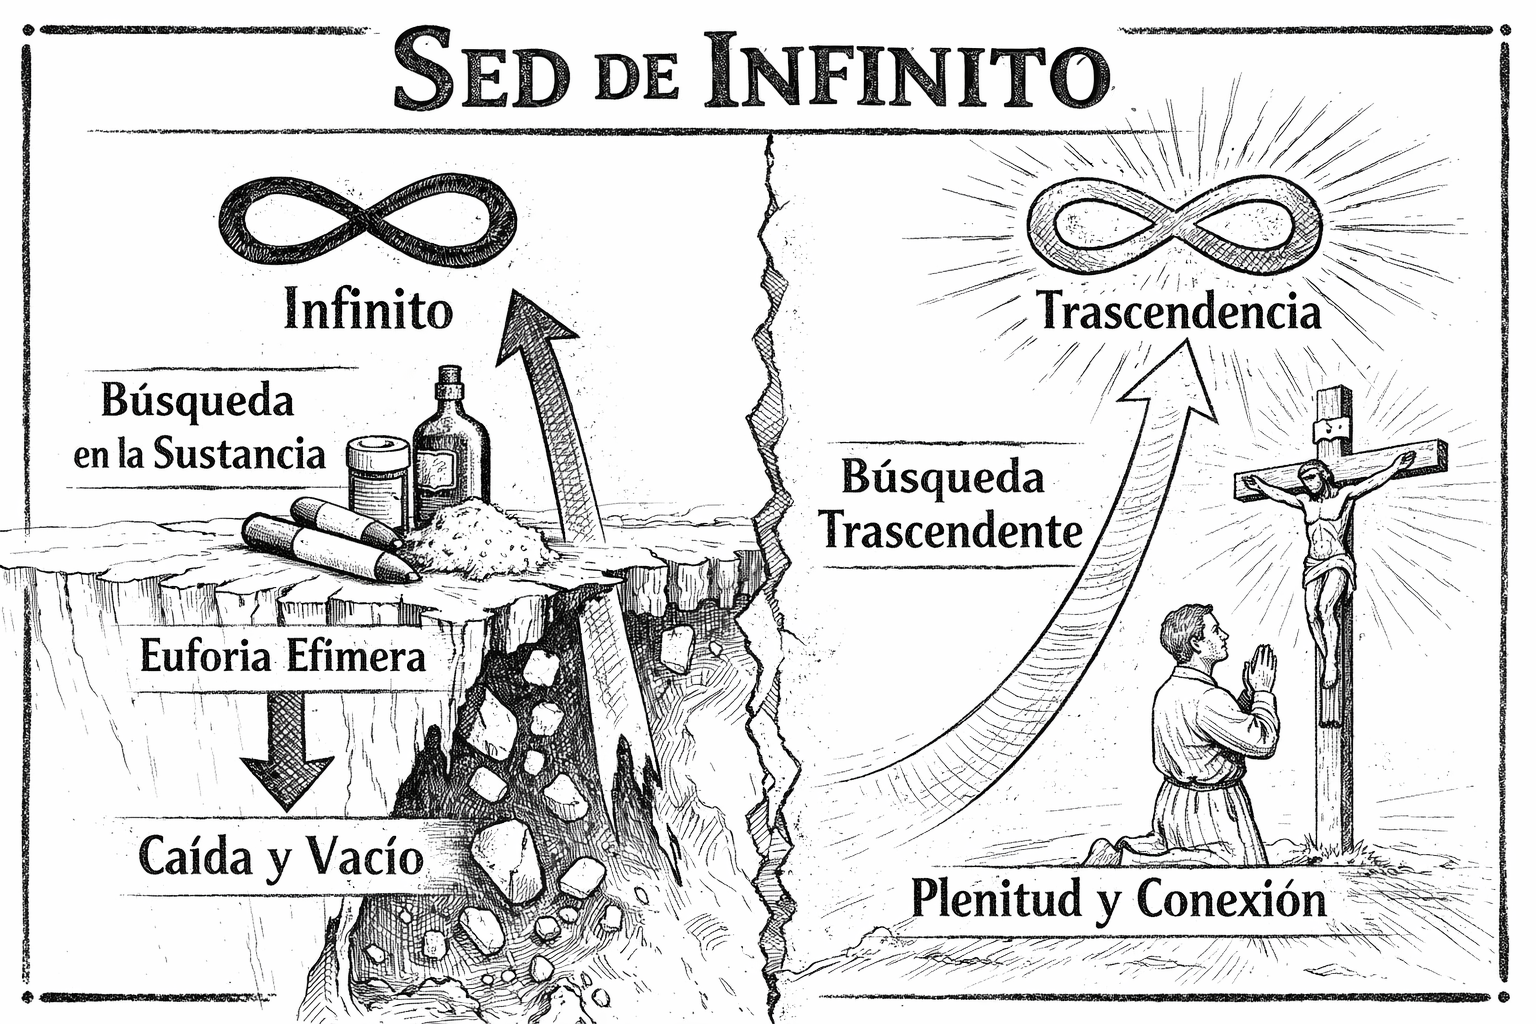
\includegraphics[scale=0.25]{232.png}
		\caption{La busqueda fallida}
	\end{figure}
	
	\momento{Fundamento o criterio de discernimiento}
	
	\marginnote{Cfr. art. 9.4.3 (sistema de recompensa y wanting)}
	
	Se afirma que el ser humano posee una estructura interna que reclama significado. La adicción representa un desencuentro con esa finalidad, donde el sujeto intenta saciar una sed de infinito con respuestas materiales. El amor se reconoce como el medicamento que permite la restauración del ser frente a este intento fallido de reparación.
	
	\momento{Tesis y desarrollo argumental}\\
	Respondemos que la adicción es una respuesta errónea a una necesidad espiritual legítima:
	\begin{itemize}
		\item \textbf{Sutura de la orfandad:} La sustancia se presenta como la única posibilidad de resistir en contextos de extrema vulnerabilidad, intentando compensar mecánicamente lo que solo el vínculo humano y el testimonio pueden sanar.
		\item \textbf{Sed de infinito mal encauzada:} En lugar de elevar al hombre, la droga lo encierra en un ciclo de soledad. La recuperación consiste en remover los obstáculos que bloquean el deseo de vivir para que la reconexión fluya.
	\end{itemize}
	
	\momento{Respuesta a las objeciones}
	\begin{itemize}
		\item \submomento{A la primera:} La ciencia explica la maquinaria del daño, pero la espiritualidad explica la causa profunda. El daño cerebral explica por qué es difícil frenar, pero la fractura interna explica por qué se sintió la necesidad de acelerar hacia el consumo como una huida del dolor.
		\item \submomento{A la segunda:} Comprender el componente anestésico no quita responsabilidad, sino que la sitúa en un marco de justicia y misericordia. El objetivo es que el hermano, mediante la escucha activa, reconozca su herida para poder elegir un proyecto de vida donde el consumo ya no sea necesario.
	\end{itemize}
	
	\subsection{Artículo 3: La desconexión con la realidad interior y con Dios en el trastorno por uso de sustancias}
	
	\momento{Planteo del tema}\\
	El trastorno por uso de sustancias no se limita a una afectación orgánica, sino que alcanza la capacidad de amar y la apertura a lo divino. Resulta necesario clarificar si esta patología constituye una fractura real en el vínculo con la propia interioridad o si es simplemente una conducta desadaptativa sin impacto en el núcleo del ser.
	
	\momento{Pregunta central}\\
	¿De qué manera el trastorno por uso de sustancias provoca una desconexión progresiva con la realidad interior y con Dios?
	
	\momento{Posturas u objeciones existentes}
	\begin{itemize}
		\item \submomento{Objeción 1:} Muchos usuarios mantienen una funcionalidad social, lo que sugeriría que el consumo no interrumpe necesariamente su vida interior ni su percepción de la realidad.
		\item \submomento{Objeción 2:} Si la relación con Dios es imborrable, no puede existir una «desconexión» real, ya que el hombre siempre permanece abierto a lo divino por naturaleza.
	\end{itemize}
	
	\momento{Fundamento o criterio de discernimiento}\\
	Se reconoce que el espíritu es la dimensión que más lentamente se recupera, pues es el eje de la renovación del alma. El trastorno causa un desencuentro progresivo con la verdad espiritual, sumiendo al hermano en un ciclo de desolación que distorsiona todas sus relaciones humanas.
	
	\momento{Tesis y desarrollo argumental}\\
	Respondemos que el trastorno por uso de sustancias fractura la unidad de la persona:
	\begin{itemize}
		\item \textbf{Pérdida de sintonía:} El distanciamiento de la propia esencia no ocurre de forma súbita, sino que aumenta con la severidad del consumo, generando un vacío que el individuo intenta colmar con más sustancia, agravando la desvitalización.
		\item \textbf{Alteración de la seguridad:} Las vivencias traumáticas llevan al sujeto a percibir el mundo como una amenaza. La sustancia actúa como un velo que lo separa de su centro unificador y del Dios que se manifiesta en la serenidad.
	\end{itemize}
	
	\momento{Respuesta a las objeciones}
	\begin{itemize}
		\item \submomento{A la primera:} La funcionalidad externa puede ocultar un deterioro profundo. La falta de conexión espiritual se manifiesta como una incapacidad progresiva de amar desinteresadamente o de encontrar un propósito que trascienda la máscara social.
		\item \submomento{A la segunda:} Es vital distinguir entre la potencia (la marca imborrable de Dios) y la condición (el estado dinámico de la relación). El consumo puede nublar u oscurecer la conciencia de la presencia divina sin borrarla; por ello, la recuperación requiere una escucha activa que ayude a retirar ese velo.
	\end{itemize}
	
	\subsection{Artículo 4: La instalación de la adicción en el vacío de sentido y la desprotección social}
	
	\marginnote{Ecl 1, 2.14\label{ecl1.2} — \textit{Vanidad de vanidades, todo es vanidad... vi todas las obras que se hacen bajo el sol y, ciertamente, todo era vanidad y atrapar vientos}}
	
	\momento{Planteo del tema}\\
	El ser humano posee exigencias originales de felicidad; sin embargo, en contextos de exclusión extrema, se produce una fractura interna. Resulta imperativo comprender si la adicción es la causa de este vacío o si es una respuesta fallida provocada por la desprotección del entorno familiar y social.
	
	\momento{Pregunta central}\\
	¿De qué manera se instala la adicción en el vacío de sentido generado por la desprotección social y la falta de pertenencia?
	
	\momento{Posturas u objeciones existentes}
	\begin{itemize}
		\item \submomento{Objeción 1:} Atribuir la problemática a factores externos de desprotección podría desdibujar la responsabilidad individual, reduciendo al sujeto a una víctima pasiva de su contexto histórico.
		\item \submomento{Objeción 2:} La curiosidad o la presión de grupo son decisiones operativas que sugieren que el trastorno nace de la voluntad y no necesariamente de una falta de raíces sociales previas.
	\end{itemize}
	
	\momento{Fundamento o criterio de discernimiento}\\
	Se establece que la dignidad permanece intacta, pero el estado espiritual se ve herido cuando la comunidad no logra ser un puerto seguro. La sanación integral requiere abordar tanto la fragilidad del individuo como la injusticia de las estructuras que generan el descarte social.
	
	\momento{Tesis y desarrollo argumental}\\
	Respondemos que la adicción compensa carencias profundas de protección:
	\begin{itemize}
		\item \textbf{Desarrollo reactivo:} Cuando el entorno no provee un apego seguro, se genera una personalidad defensiva que busca alivio en la gratificación inmediata, instalándose en la grieta que la sociedad no supo cubrir.
		\item \textbf{Invisibilidad social:} En contextos de vulnerabilidad, la droga llena falsamente la necesidad de propósito. El trastorno es la búsqueda compulsiva de una vivencia para escapar de un presente sin esperanza ni redes de apoyo.
	\end{itemize}
	
	\momento{Respuesta a las objeciones}
	\begin{itemize}
		\item \submomento{A la primera:} Reconocer la fractura interna no quita responsabilidad, sino que la sitúa en un marco de justicia. El objetivo es que la comunidad remueva los obstáculos del abandono para que el hermano pueda recuperar el protagonismo de su vida mediante el diálogo fraterno.
		\item \submomento{A la segunda:} En contextos de alta vulnerabilidad, lo que comienza como curiosidad se transforma en estrategia de supervivencia. La falta de cimientos sociales fuertes hace que el sujeto no tenga de dónde asirse para frenar el impulso, requiriendo el ancla de una comunidad que ofrezca testimonio y seguridad.
	\end{itemize}
	
	\subsection{Artículo 5: El consumismo como «evangelio del bienestar» y motor de la desconexión espiritual}
	
	\momento{Planteo del tema}\\
	El consumismo se ha erigido como un sistema de creencias que promete felicidad inmediata, compitiendo directamente con la búsqueda de sentido. Es necesario juzgar si esta promesa es una solución real o si es el motor que profundiza la desconexión de la persona con su interioridad y con lo trascendente.
	
	\momento{Pregunta central}\\
	¿En qué medida el consumismo actúa como un evangelio del bienestar que ofrece soluciones mágicas que agravan la desconexión espiritual?
	
	\momento{Posturas u objeciones existentes}
	\begin{itemize}
		\item \submomento{Objeción 1:} La búsqueda de bienestar es una inclinación natural hacia el placer, por lo que el consumo de bienes y sensaciones es biológicamente adaptativo y no una causa de desconexión espiritual.
		\item \submomento{Objeción 2:} Los problemas de adicción son enfermedades neurobiológicas que no dependen de factores culturales o ideológicos como el consumismo.
	\end{itemize}
	
	\momento{Fundamento o criterio de discernimiento}\\
	El juicio espiritual reconoce que la verdadera plenitud no puede ser comprada. La reducción de la esperanza a la posesión material genera una desvitalización del espíritu, reforzando la dependencia mediante la oferta de un «instante mágico» que nunca sacia la sed profunda de infinito.
	
	\momento{Tesis y desarrollo argumental}\\
	Respondemos que el consumismo es una ideología que agrava la fractura interna:
	\begin{itemize}
		\item \textbf{Solución mágica:} Se propone la satisfacción inmediata como valor supremo, convirtiendo a la sustancia en un falso absoluto que suplanta la verdadera trascendencia y el esfuerzo del crecimiento personal.
		\item \textbf{Corrosión del tejido social:} Al priorizar el «tener» sobre el «ser», el sujeto queda aislado en su consumo, perdiendo la red de pertenencia que es el ancla fundamental de la recuperación y la salud.
	\end{itemize}
	
	\momento{Respuesta a las objeciones}
	\begin{itemize}
		\item \submomento{A la primera:} El bienestar auténtico no es solo la liberación de dopamina\marginnote{Cfr. art.~\ref{art:dopamina} (Juzgar, Las sustancias y el organismo, La farmacodinámica..., Art. 1...)}, sino la realización integral en comunidad. El consumismo confunde el deseo momentáneo con la necesidad de significado, lo que tarde o temprano se manifiesta como desolación.
		\item \submomento{A la segunda:} Aunque la adicción altere el cerebro, los factores culturales determinan si una persona recurre a las sustancias para anestesiar una vida que el sistema de mercado ha vuelto intolerable. El proceso de salud requiere un diálogo fraterno que ayude a distinguir el valor del ser frente a la lógica del tener.
	\end{itemize}
	
	\newpage
	
	\section{El proceso de reconexión}
	
	El proceso de reconexión se define como un flujo natural y espontáneo que se manifiesta en el encuentro con Dios y con la comunidad bajo el marco de un amor responsable. Partiendo de la premisa de que el trastorno por uso de sustancias genera un desencuentro o desconexión progresiva con la realidad espiritual interior, el trabajo de recuperación no consiste en forzar el cambio conductual mediante la imposición, sino en remover los obstáculos que bloquean dicho flujo. A través del camino espiritual y el discernimiento, se busca que el sujeto sane su historia vincular para recuperar sus funciones más elevadas. En última instancia, la reconexión permite que la persona pase de un estado de desolación a una confianza renovada en el porvenir, reconociéndose nuevamente como un ser valioso, único e irrepetible.
	
	\subsection{Artículo 1: La espontaneidad de la reconexión espiritual en el encuentro con Dios y los hermanos}
	
	\marginnote{Lc 15, 17\label{lc15.17} — \textit{Entonces, recapacitando, dijo: ¿Cuántos jornaleros de mi padre tienen pan en abundancia, mientras que yo aquí me muero de hambre?}}
	
	\momento{Planteo del tema}\\
	Frente a la problemática del consumo, a menudo se considera que la recuperación es exclusivamente el resultado de un esfuerzo titánico de la voluntad o de una técnica psicológica compleja. Sin embargo, la perspectiva de la Iglesia sostiene que la dimensión espiritual posee un dinamismo propio que tiende hacia la salud. Resulta necesario discernir si la reconexión con el sentido de la vida es una construcción artificial o un flujo natural que brota cuando se restablecen los vínculos fundamentales con el creador y la comunidad.
	
	\momento{Pregunta central}\\
	¿Por qué se afirma que la reconexión espiritual se da de forma espontánea en el encuentro con Dios y los hermanos?
	
	\momento{Posturas u objeciones existentes}
	\begin{itemize}
		\item \submomento{Objeción 1:} El cambio de conducta requiere una motivación alta y constante que exige un esfuerzo consciente y voluntario, por lo que no podría ser un proceso espontáneo.
		\item \submomento{Objeción 2:} El consumo de sustancias genera una desconexión tan profunda que se requeriría una intervención externa impositiva para reparar la visión de la persona.
	\end{itemize}
	
	\momento{Fundamento o criterio de discernimiento}\\
	Se establece que el encuentro con la trascendencia en un marco de amor responsable permite que la fuerza de la reconexión opere mediante un flujo natural. El espíritu humano posee una inclinación intrínseca hacia el bienestar y la verdad; por lo tanto, no es necesario fabricar la espiritualidad, sino manifestarla mediante la acogida y la seguridad vincular.
	
	\momento{Tesis y desarrollo argumental}\\
	Respondemos que la reconexión espiritual es espontánea porque responde a la naturaleza relacional del ser humano:
	\begin{itemize}
		\item \textbf{Esencia relacional del ser:} La persona se realiza en el vínculo. Al producirse un encuentro genuino, el espíritu reconoce su entorno natural y la reconexión fluye sin necesidad de artificios técnicos, apoyándose en el testimonio de los otros.
		\item \textbf{Abandono en un Poder Superior:} La reconexión se activa cuando la persona acepta su fragilidad. En ese acto de confianza, el encuentro con la gracia activa una sanación profunda que trasciende el puro esfuerzo voluntarista.
	\end{itemize}
	
	\momento{Respuesta a las objeciones}
	\begin{itemize}
		\item \submomento{A la primera:} Aunque la motivación fluctúe, la comunidad actúa como un motor de esperanza externo que sostiene al sujeto. La espontaneidad no significa ausencia de esfuerzo, sino que el impulso para ese esfuerzo nace de un deseo interno recuperado y no de una presión externa.
		\item \submomento{A la segunda:} La chispa espiritual no se enciende por imposición, sino cuando la persona se siente valorada en su identidad. El reconocimiento del valor propio, mediado por la escucha activa, es lo que revierte naturalmente la desconexión provocada por la sustancia.
	\end{itemize}
	
	\subsection{Artículo 2: Los obstáculos a la reconexión espiritual y su remoción mediante el discernimiento}
	
	\momento{Planteo del tema}\\
	Aunque el espíritu posee un dinamismo hacia la salud, observamos que este flujo a menudo parece detenido por el peso de la desolación. Para que la recuperación sea efectiva, no basta con proponer metas externas; es necesario discernir qué elementos actúan como una barrera interna. Comprender estos impedimentos permite que la comunidad actúe para limpiar el cauce de la vida interior y facilitar la reconexión del hermano con su propósito vital.
	
	\momento{Pregunta central}\\
	¿Cuáles son los obstáculos que bloquean el flujo natural de la reconexión espiritual y de qué manera pueden removerse mediante el discernimiento?
	
	\momento{Posturas u objeciones existentes}
	\begin{itemize}
		\item \submomento{Objeción 1:} Dado que la relación con lo trascendente es un constitutivo inalienable, nada en el plano psicológico o social debería poder obstaculizar un don de origen divino.
		\item \submomento{Objeción 2:} El discernimiento es una función racional compleja que requiere de una integridad cognitiva que el consumo suele dañar, impidiendo que el sujeto participe activamente.
	\end{itemize}
	
	\momento{Fundamento o criterio de discernimiento}\\
	El trabajo de restauración consiste en identificar los factores que bloquean el dinamismo del espíritu. Se reconoce que la dimensión espiritual puede verse afectada por carencias afectivas extremas. El criterio pastoral busca generar las condiciones vinculares necesarias para que la potencia del ser vuelva a manifestarse tras remover los obstáculos del abandono.
	
	\momento{Tesis y desarrollo argumental}\\
	Respondemos que la vivencia de la trascendencia se ve condicionada por obstáculos que requieren una pedagogía de la proximidad:
	\begin{itemize}
		\item \textbf{Obstáculos principales:} La desprotección genera un vacío de sentido que el sujeto intenta cubrir con sustancias. El estigma social alimenta un sentimiento de no merecimiento, provocando una fractura interna que bloquea el deseo de mejora.
		\item \textbf{Remoción mediante el camino espiritual:} La cultura del encuentro ofrece seguridad, mientras que la vida sacramental ayuda a romper el ciclo de la culpa, permitiendo que la persona se sienta valorada nuevamente.
	\end{itemize}
	
	\momento{Respuesta a las objeciones}
	\begin{itemize}
		\item \submomento{A la primera:} La dignidad ontológica permanece intacta, pero la conciencia de esa dignidad se nubla por el dolor. Remover obstáculos no crea la luz espiritual, sino que quita el velo de la desolación para que esa luz ilumine la vida concreta del sujeto.
		\item \submomento{A la segunda:} El discernimiento\index{discernimiento|textbf} en la Iglesia no es un ejercicio intelectual solitario, sino un arte del acompañamiento compartido. La comunidad presta su capacidad de juzgar y esperar al hermano mediante el diálogo fraterno, sosteniéndolo hasta que recupere su autonomía.
	\end{itemize}
	
	\subsection{Artículo 3: El despertar espiritual como chispa de vida nueva y digna}
	
	\marginnote{Ef 5, 14\label{ef5.14} — \textit{Despierta tú que duermes, levántate de entre los muertos, y Cristo te iluminará}}
	
	\momento{Planteo del tema}\\
	En el acompañamiento se observa a menudo un estado de desvitalización donde el sujeto parece haber perdido el motor interno. Debemos discernir si la transformación nace de un mero esfuerzo de la voluntad o si existe una chispa que se enciende al recuperar la conciencia del propio valor. Comprender este despertar permite a la comunidad actuar como el entorno que facilita que esta nueva luz guíe los pasos del hermano hacia una vida con propósito.
	
	\momento{Pregunta central}\\
	¿De qué manera actúa el despertar espiritual como la chispa que enciende el deseo de una vida nueva y digna en el hermano que sufre?
	
	\momento{Posturas u objeciones existentes}
	\begin{itemize}
		\item \submomento{Objeción 1:} El cambio en la conducta adictiva se explica exclusivamente por la neuroplasticidad\marginnote{Cfr. art.~\ref{art:neuroplasticidad} (Juzgar, Brevísimo Glosario)} cerebral, por lo que apelar a un despertar espiritual resulta innecesario para la ciencia.
		\item \submomento{Objeción 2:} La voluntad de las personas con trastorno por uso de sustancias está profundamente dañada; por tanto, una chispa interna sería insuficiente para vencer la compulsión.
	\end{itemize}
	
	\momento{Fundamento o criterio de discernimiento}\\
	Se establece que cuando una persona logra reconectarse con su sentido y su historia, se produce un movimiento interno que abre caminos de esperanza. Este despertar es una experiencia afectiva donde el sujeto se reconoce como un ser sagrado. La fe actúa como la energía que transforma la percepción de un mundo hostil en un espacio de posibilidad.
	
	\momento{Tesis y desarrollo argumental}\\
	Respondemos que el despertar espiritual es la chispa fundamental para la vida nueva mediante estos procesos:
	\begin{itemize}
		\item \textbf{Reconocimiento del valor esencial:} La chispa se enciende cuando la persona descubre que su identidad no está definida por sus errores. Al reconocerse portador de una marca divina, el hermano deja de verse como un descarte social.
		\item \textbf{Activación de la resiliencia en comunidad:} Este encendido ocurre al sentirse acogido. El ambiente de afecto incondicional rompe el ciclo del miedo, permitiendo que la fractura interna comience a sanar mediante el testimonio de los otros.
	\end{itemize}
	
	\momento{Respuesta a las objeciones}
	\begin{itemize}
		\item \submomento{A la primera:} La ciencia describe la maquinaria biológica, pero la espiritualidad es la que otorga el significado y el para qué necesario para que esa maquinaria se ponga en marcha hacia un fin que trascienda la mera supervivencia física.
		\item \submomento{A la segunda:} Aunque la voluntad esté debilitada, el despertar espiritual depende de la ayuda recibida. El vínculo afectivo y la escucha activa reparan la voluntad, ofreciendo una fuerza que el sujeto por sí solo no podría generar inicialmente.
	\end{itemize}
	
	\subsection{Artículo 4: La recuperación de la autonomía y la gestión responsable del proyecto vital}
	
	\momento{Planteo del tema}\\
	En el acompañamiento se observa a menudo una fuerte dependencia institucional. La autonomía surge como el nivel más alto de independencia y toma de decisiones informadas del que el sujeto es capaz. Es imperativo juzgar cómo esta potencia se traduce en una gestión responsable que permita al hermano transitar de ser un asistido a ser un ciudadano activo y protagonista en su comunidad.
	
	\momento{Pregunta central}\\
	¿De qué forma la recuperación de la autonomía permite al sujeto independizarse de la dependencia institucional a través de la gestión responsable de su vida?
	
	\momento{Posturas u objeciones existentes}
	\begin{itemize}
		\item \submomento{Objeción 1:} El deterioro cognitivo y de voluntad impediría a estas personas tomar las riendas de su vida sin una supervisión institucional constante y permanente.
		\item \submomento{Objeción 2:} Al abandonar el entorno protegido, la falta de una estructura externa rígida conduce inevitablemente al fracaso del proceso debido a la exposición al mercado.
	\end{itemize}
	
	\momento{Fundamento o criterio de discernimiento}\\
	La recuperación es un proceso autodirigido donde la persona es el agente principal. El éxito del proceso espiritual es el desarrollo del máximo potencial del individuo para llevar una vida autónoma. La comunidad no debe sustituir la voluntad del hermano, sino fortalecer su capacidad de autodirección hacia su destino final.
	
	\momento{Tesis y desarrollo argumental}\\
	Respondemos que la autonomía permite la independencia institucional mediante un proceso de maduración progresiva:
	\begin{itemize}
		\item \textbf{Gestión material como herramienta:} La reeducación financiera y el manejo de recursos permiten reemplazar el patrón impulsivo por la planificación. Esto facilita el acceso a la vivienda y al autosostenimiento fuera de la institución.
		\item \textbf{El protagonismo en el proyecto vital:} El sujeto deja de ser un espectador. Este empoderamiento espiritual implica que la persona asuma la responsabilidad de su bienestar, participando en un diálogo fraterno con su entorno social.
	\end{itemize}
	
	\momento{Respuesta a las objeciones}
	\begin{itemize}
		\item \submomento{A la primera:} Aunque existan secuelas, la neuroplasticidad\marginnote{Cfr. art.~\ref{art:neuroplasticidad} (Juzgar, Brevísimo Glosario)} y el acompañamiento de pares permiten aprender nuevos repertorios de gestión personal. La autonomía es progresiva y se entrena en la práctica cotidiana del cuidado de la vida propia.
		\item \submomento{A la segunda:} La independencia no significa aislamiento absoluto. El modelo contempla que la persona mantenga vínculos de pertenencia y redes de escucha activa con su comunidad de origen, lo que previene recaídas mediante la seguridad de no estar solo.
	\end{itemize}
	
	\newpage
	
	\section{El camino cristiano}
	
	El camino cristiano se presenta como una propuesta de sanación y libertad que trasciende lo puramente clínico, centrando su eje en el encuentro personal con Jesucristo. Este recorrido se fundamenta en una Iglesia en salida\index{iglesia en salida} que actúa como un refugio dispuesto a recibir la vida como viene. Lejos de ser un conjunto de normas rígidas, propone una espiritualidad encarnada donde la comunidad se transforma en una familia que acompaña el dolor sin juzgar. A través de la misericordia y la vivencia de la palabra, el proceso busca remover los obstáculos del alma para que la persona recupere su capacidad de amar y de trascender, encendiendo la chispa de un proyecto de vida con sentido.
	
	\subsection{Artículo 1: El anuncio de la fe en relación con el abordaje técnico-profesional}
	
	\momento{Planteo del tema}\\
	Surge a menudo la tensión entre la confianza en el poder transformador del mensaje cristiano y la necesidad de recurrir a las herramientas de la medicina o la psicología. Es fundamental discernir si el anuncio del amor de Dios invalida el trabajo clínico o si ambas dimensiones deben articularse en una unidad de sentido para la restauración integral de la persona que padece un trastorno por uso de sustancias.
	
	\momento{Pregunta central}\\
	¿De qué manera el anuncio de la fe se articula con el abordaje técnico-profesional en el proceso de salud integral?
	
	\momento{Posturas u objeciones existentes}
	\begin{itemize}
		\item \submomento{Objeción 1:} Si el amor es el medicamento supremo, el anuncio de la fe debería ser suficiente por sí solo, haciendo innecesaria la intervención técnica o farmacológica.
		\item \submomento{Objeción 2:} Dado que la adicción es una afección del espíritu, una solución técnica resulta superficial, mientras que la fe llegaría a la raíz misma del problema.
	\end{itemize}
	
	\momento{Fundamento o criterio de discernimiento}\\
	La Iglesia evita la tentación de un espiritualismo que ignore las realidades físicas y psíquicas. La intervención es un proceso integral donde lo biológico y lo espiritual son ingredientes necesarios pero insuficientes si se aplican de forma aislada.\index{integralidad|textbf} La salud es el despliegue del máximo potencial de la persona, lo que exige una colaboración armoniosa entre la sabiduría de la fe y el saber de la ciencia.
	
	\momento{Tesis y desarrollo argumental}\\
	Respondemos que no existe superioridad en términos de exclusión, sino una complementariedad necesaria:
	\begin{itemize}
		\item \textbf{La fe como fundamento del sentido:} La fe otorga el para qué de la recuperación. Devuelve al sujeto su identidad profunda, permitiéndole pasar de la desolación a la esperanza.
		\item \textbf{El abordaje técnico como mediación:} La ciencia proporciona los medios para tratar la maquinaria biológica dañada. Ignorar la biología sería una falta de responsabilidad pastoral; la intervención profesional estabiliza al hermano para que su espíritu recupere la capacidad de decidir.
	\end{itemize}
	
	\momento{Respuesta a las objeciones}
	\begin{itemize}
		\item \submomento{A la primera:} El amor de Dios también se manifiesta a través del don de la ciencia. Dios sana frecuentemente mediante mediaciones humanas; rechazar el abordaje técnico sería desestimar las herramientas que la providencia pone a disposición para el cuidado de la vida.
		\item \submomento{A la segunda:} Aunque la adicción afecte el núcleo del ser, se encarna en el sistema nervioso. El cuidado de la salud física dispone al espíritu para recibir el mensaje de esperanza mediante la formación de nuevos vínculos en un diálogo fraterno.
	\end{itemize}
	
	\subsection{Artículo 2: La importancia del primer anuncio en el despertar espiritual del hermano}
	
	\momento{Planteo del tema}\\
	En el acompañamiento, a menudo se prioriza la estabilización biológica. Sin embargo, surge el interrogante sobre la eficacia de un mensaje espiritual en sujetos que han perdido el sentido de su propia valía. Es fundamental discernir si el mensaje de que Dios ama incondicionalmente al ser humano es una pieza central en el proceso de salud o un elemento secundario.
	
	\momento{Pregunta central}\\
	¿Qué importancia tiene el primer anuncio para despertar una dimensión espiritual herida por el consumo problemático?
	
	\momento{Posturas u objeciones existentes}
	\begin{itemize}
		\item \submomento{Objeción 1:} El trastorno altera las funciones ejecutivas, por lo que un mensaje espiritual no tendría capacidad de reparar daños neurológicos ni frenar el impulso biológico.
		\item \submomento{Objeción 2:} En personas con dificultades para acatar límites, un mensaje de amor incondicional y falta de juicio podría fomentar la irresponsabilidad conductual.
	\end{itemize}
	
	\begin{figure}[h!]
		\centering
		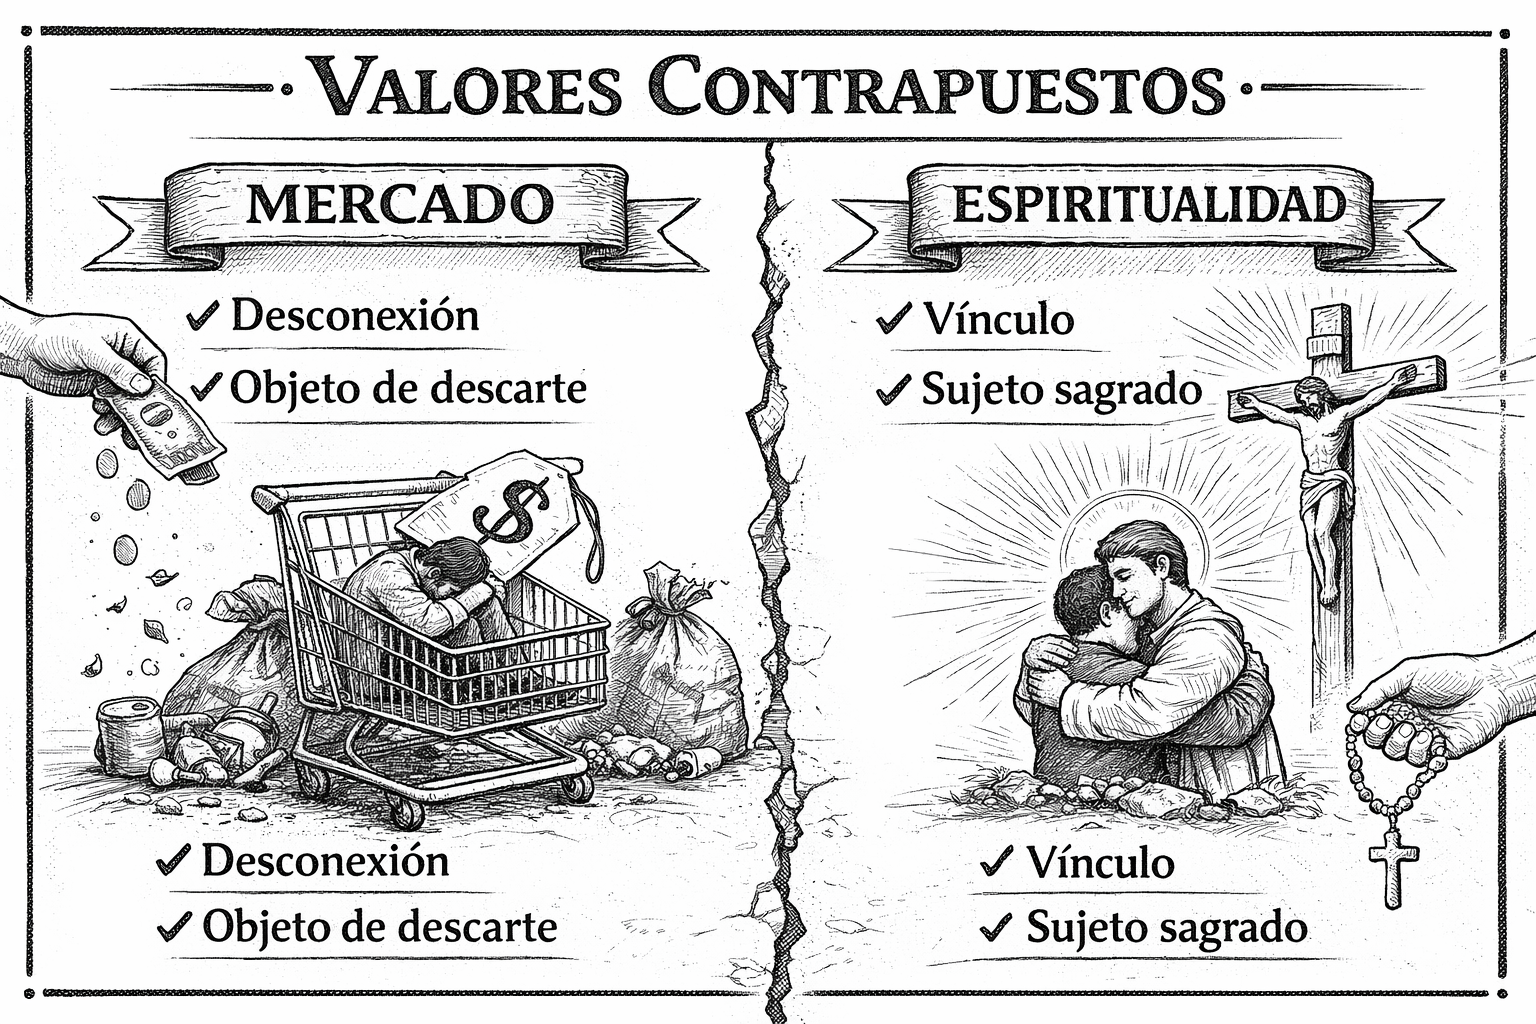
\includegraphics[scale=0.25]{252.png}
		\caption{Los valores de la espiritualidad}
	\end{figure}
	
	\momento{Fundamento o criterio de discernimiento}\\
	El mensaje central de la fe actúa como la chispa que enciende el deseo de una vida nueva. No es una doctrina abstracta, sino un encuentro que rescata a la persona de su desvitalización. Al devolver al sujeto la conciencia de que su vida es sagrada, la fe se convierte en la energía necesaria para ser protagonista de su propia historia.
	
	\momento{Tesis y desarrollo argumental}\\
	\begin{itemize}
		\item \textbf{Sanación de la fractura interna:} El amor incondicional responde a la orfandad profunda. Al saberse amado más allá de su comportamiento, el sujeto deja de verse como un descarte para reconocerse como un hijo.
		\item \textbf{Ruptura del ciclo de la culpa:} El anuncio de que Dios no juzga es vital para desarmar el autodesprecio. La experiencia del perdón permite separar el valor esencial de los errores pasados.
	\end{itemize}
	
	\momento{Respuesta a las objeciones}
	\begin{itemize}
		\item \submomento{A la primera:} Mientras la ciencia repara la maquinaria, la espiritualidad otorga la motivación trascendente para sostener ese proceso. El propósito vital utiliza la neuroplasticidad\marginnote{Cfr. art.~\ref{art:neuroplasticidad} (Juzgar, Brevísimo Glosario)} para fortalecer el compromiso con el tratamiento médico.
		\item \submomento{A la segunda:} La misericordia hace posible la responsabilidad. Solo quien se siente verdaderamente digno es capaz de asumir la gestión de su propia vida y adherir libremente a los límites necesarios para su bienestar mediante la escucha activa.
	\end{itemize}
	
	\subsection{Artículo 3: El encuentro personal con Cristo como camino de resurrección}
	
	\momento{Planteo del tema}\\
	En la pastoral, el dolor no es un callejón sin salida, sino el lugar donde la fragilidad se encuentra con la gracia. Debemos discernir si el encuentro con Cristo constituye una verdadera transformación que devuelve la vida a lo que parecía perdido, abriendo un camino de esperanza frente a la desolación del consumo.
	
	\momento{Pregunta central}\\
	¿De qué manera el encuentro personal con Cristo transforma el dolor en un camino de resurrección?
	
	\momento{Posturas u objeciones existentes}
	\begin{itemize}
		\item \submomento{Objeción 1:} El dolor está anclado en daños biológicos objetivos; un encuentro espiritual no puede revertir por sí solo la fisiología del cerebro.
		\item \submomento{Objeción 2:} Hablar de resurrección parece una exageración lírica frente a trayectorias de vida marcadas por la reincidencia, el hospital o la cárcel.
	\end{itemize}
	
	\momento{Fundamento o criterio de discernimiento}\\
	El amor es el medicamento supremo. Amar a alguien en Cristo es ofrecerle una posibilidad real de vida nueva. La resurrección es una fuerza actual que permite que lo que estaba muerto por el consumo vuelva a florecer mediante la confianza y el vínculo comunitario.
	
	\momento{Tesis y desarrollo argumental}\\
	\begin{itemize}
		\item \textbf{Revelación de la identidad sagrada:} Al verse a través de los ojos de Cristo, la persona deja de ser una cifra para reconocerse como un ser valioso. Esta es la chispa necesaria para iniciar la reconstrucción.
		\item \textbf{Cristo como médico que asume la llaga:} Jesús toca la carne sufriente e involucra su vida en la desolación del hermano. Al identificarse con el crucificado, el doliente comprende que su fragilidad es el punto de encuentro con una fuerza superior.
	\end{itemize}
	
	\momento{Respuesta a las objeciones}
	\begin{itemize}
		\item \submomento{A la primera:} La resurrección proporciona el para qué vivir que la medicina sola no puede dar, motivando al sujeto a comprometerse con su salud integral y a ejercer su libertad recuperada mediante el testimonio.
		\item \submomento{A la segunda:} La resurrección en este contexto no se mide por la ausencia de caídas, sino por la capacidad de ponerse de pie. Es el triunfo de la esperanza que afirma que, incluso en el límite, el ser humano conserva la potencia de comenzar de nuevo.
	\end{itemize}
	
	\subsection{Artículo 4: El valor del testimonio y la escucha activa en la generación de confianza}
	
	\momento{Planteo del tema}\\
	En el acompañamiento de personas marcadas por el estigma, el rechazo social suele fracturar la capacidad de confiar. La comunidad debe discernir si el uso de la palabra posee la potencia necesaria para sanar este vínculo dañado o si se requiere únicamente de intervenciones técnicas estandarizadas.
	
	\momento{Pregunta central}\\
	¿De qué manera el testimonio y la escucha activa generan la confianza necesaria para la recuperación en quienes han vivido bajo el peso del rechazo?
	
	\momento{Posturas u objeciones existentes}
	\begin{itemize}
		\item \submomento{Objeción 1:} El abordaje debe ser primariamente científico; los relatos de experiencias personales carecen de rigor para modificar una afección biológica.
		\item \submomento{Objeción 2:} La escucha es un método subjetivo que no resuelve las necesidades materiales básicas, que son la verdadera urgencia del hermano.
	\end{itemize}
	
	\momento{Fundamento o criterio de discernimiento}
	
	\marginnote{Cfr. La escucha activa y el trabajo interior del acompañante (cap. 8)}
	
	La escucha activa\index{escucha|textbf} es el primer medicamento en la restauración del alma. El objetivo es crear una atmósfera de hospitalidad donde la persona se exprese con libertad. El testimonio no busca imponer una doctrina, sino ofrecer un reflejo de esperanza que invite al otro a plantear su propia respuesta vital.
	
	\momento{Tesis y desarrollo argumental}\\
	\begin{itemize}
		\item \textbf{El acompañante par como referente:} El testimonio de quien ya transitó el sufrimiento genera una legitimidad única. El hermano confía porque el otro conoce la realidad del territorio; su vida es la prueba de que es posible levantarse.
		\item \textbf{La escucha que dignifica:} Prestar atención al corazón del otro, creyendo que su palabra es valiosa, desarma la actitud defensiva. El sujeto baja su coraza y comienza a reconocer su propio valor intrínseco.
		\item \textbf{Habilitación de la historia personal:} El diálogo fraterno permite que el dolor se transforme en un relato coherente y este en un proyecto de vida. La persona deja de ser una cifra para ser un sujeto con nombre propio.
	\end{itemize}
	
	\momento{Respuesta a las objeciones}
	\begin{itemize}
		\item \submomento{A la primera:} Mientras la ciencia trata la maquinaria física, el testimonio es el que otorga el motivo para vivir. La técnica repara, pero la palabra compartida es la que humaniza el recorrido y permite que la salud sea integral.
		\item \submomento{A la segunda:} La escucha activa es el vínculo afectivo que permite al sujeto recuperar la confianza para aceptar la ayuda institucional. Sin este puente de humanidad, es frecuente que el hermano rechace los servicios por sentirse instrumentalizado.
	\end{itemize}
	
	\subsection{Artículo 5: La Lectio Divina como camino de confrontación y sanación espiritual}
	
	\momento{Planteo del tema}\\
	Surge el interrogante de si la lectura de los textos sagrados es un ejercicio intelectual o si posee la potencia para interpelar la biografía del sujeto. Debemos discernir cómo la palabra de Dios permite al hermano reconstruir su identidad frente al vacío de sentido que dejó el consumo.
	
	\momento{Pregunta central}\\
	¿De qué manera la Lectio Divina permite que la palabra de Dios confronte y sane la historia vital de cada persona?
	
	\momento{Posturas u objeciones existentes}
	\begin{itemize}
		\item \submomento{Objeción 1:} El trastorno genera a menudo un deterioro cognitivo que dificulta los procesos de atención necesarios para una lectura meditada.
		\item \submomento{Objeción 2:} Muchas personas en consumo sufren una fractura interna que hace que el lenguaje religioso les resulte ajeno o les genere rechazo por experiencias previas de culpa.
	\end{itemize}
	
	\begin{figure}[h!]
		\centering
		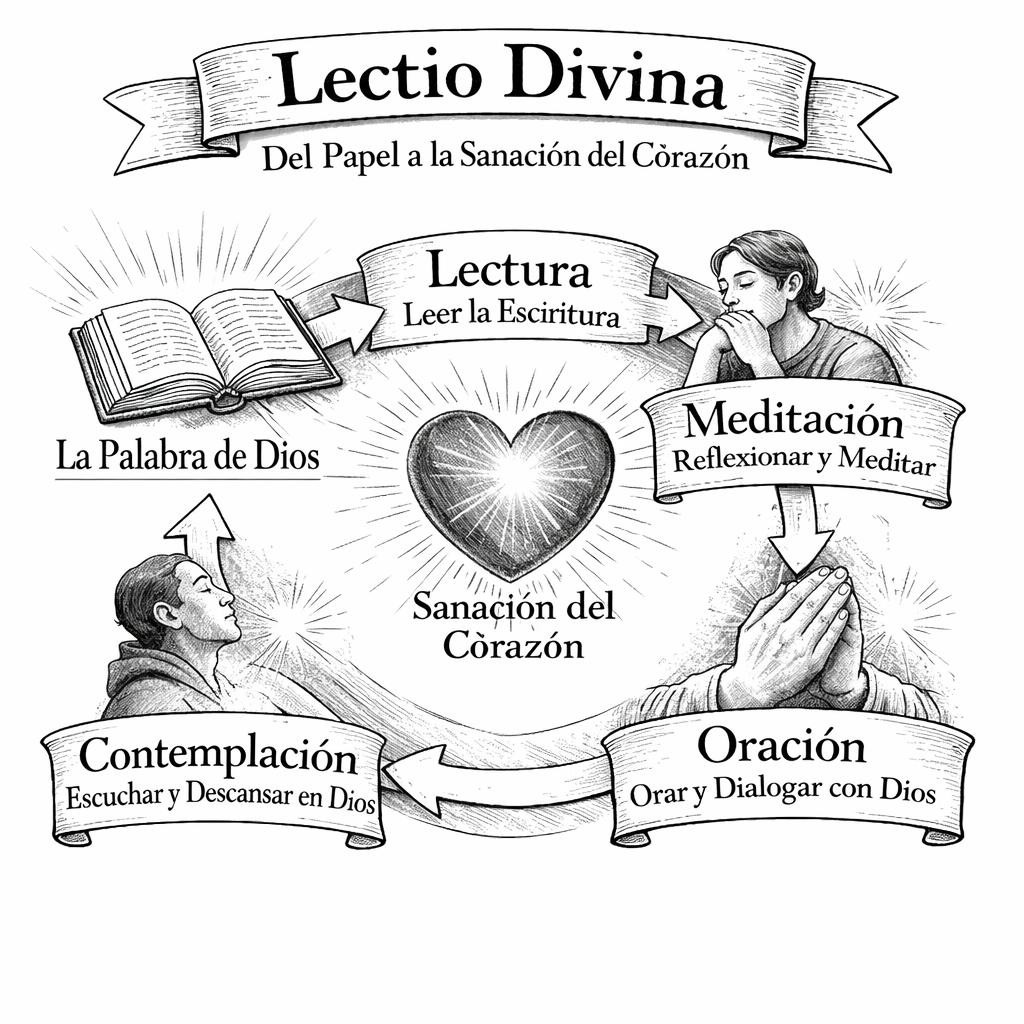
\includegraphics[scale=0.25]{255.png}
		\caption{La lectura orante de la Palabra de Dios}
	\end{figure}
	
	\momento{Fundamento o criterio de discernimiento}\\
	La lectura orante, aterrizada a la realidad, permite cuestionar las propias acciones frente al modelo de Jesús. La palabra no es una norma fría, sino una presencia que confronta el vivir diario. No se busca erudición, sino un encuentro afectivo donde la verdad se manifiesta en la sencillez.
	
	\momento{Tesis y desarrollo argumental}\\
	\begin{itemize}
		\item \textbf{Confrontación con una verdad amorosa:} La palabra desplaza las mentiras del consumo. Al ser una verdad mediada por la misericordia, el hermano se siente invitado a reconocer su dignidad y no a ser condenado.
		\item \textbf{Reprocesamiento de la memoria:} La lectura orante permite resignificar recuerdos dolorosos. Al iluminar la historia con el evangelio, la persona descubre que su vida es sagrada y que la última palabra la tiene la esperanza.
	\end{itemize}
	
	\momento{Respuesta a las objeciones}
	\begin{itemize}
		\item \submomento{A la primera:} La comprensión no es un logro intelectual, sino una experiencia del corazón. La práctica comunitaria utiliza el diálogo fraterno como mediador para que el hermano se siente alojado y seguro en el grupo.
		\item \submomento{A la segunda:} La palabra debe presentarse desde una pedagogía de la proximidad. Cuando el sujeto se siente amado incondicionalmente, la resistencia disminuye, permitiendo que la palabra sane la imagen dañada de sí mismo mediante la escucha activa.
	\end{itemize}
	
	\subsection{Artículo 6: La necesidad de una espiritualidad encarnada y relacional verificada en el servicio}
	
	\momento{Planteo del tema}\\
	Existe la tentación de considerar la recuperación como un fenómeno estrictamente privado. Resulta fundamental discernir si la espiritualidad puede sostenerse en el aislamiento o si requiere verificarse en el vínculo con los demás y en el servicio concreto para ser auténtica.
	
	\momento{Pregunta central}\\
	¿Por qué es fundamental que la espiritualidad se verifique en el servicio relacional y no en un intimismo aislado?
	
	\momento{Posturas u objeciones existentes}
	\begin{itemize}
		\item \submomento{Objeción 1:} La espiritualidad es la relación íntima entre el alma y el creador; el proceso debería ocurrir exclusivamente en la conciencia y voluntad del sujeto.
		\item \submomento{Objeción 2:} El servicio al prójimo se percibe como una actividad asistencial externa que no impacta en la rehabilitación profunda de la dimensión espiritual.
	\end{itemize}
	
	\momento{Fundamento o criterio de discernimiento}\\
	El ser humano es constitutivamente relacional. La espiritualidad no es un refugio abstracto, sino una dimensión encarnada. La verdadera salud espiritual se reconoce cuando la persona sale de su egocentrismo para encontrarse con la realidad sufriente de sus hermanos.
	
	\momento{Tesis y desarrollo argumental}\\
	\begin{itemize}
		\item \textbf{Sanación mediante el vínculo:} Dado que la adicción es un desencuentro, la respuesta es la comunión. El aislamiento se revierte mediante la integración en una comunidad que ofrece afecto. El intercambio de experiencias permite que el dolor se transforme en historia compartida.
		\item \textbf{El principio del sanador herido:} La madurez se verifica en el paso de ser un asistido a ser un servidor. Al cuidar a otro, el sujeto descubre que su historia de dolor tiene un valor salvífico, activando una resiliencia que devuelve el gusto por vivir.
	\end{itemize}
	
	\momento{Respuesta a las objeciones}
	\begin{itemize}
		\item \submomento{A la primera:} Una fe desvinculada del hermano corre el riesgo de convertirse en un misticismo que no sostiene la vida ante las crisis. El ser humano solo se descubre plenamente en el encuentro con el otro a través de la escucha activa.
		\item \submomento{A la segunda:} El servicio es el lugar donde se verifica la autenticidad del despertar espiritual. El diálogo fraterno y el compromiso con el prójimo otorgan el fundamento sólido para que la recuperación sea duradera y llena de testimonio.
	\end{itemize}
	
	\newpage
	
	\section{Los sacramentos}
	
	Los sacramentos se comprenden como encuentros vitales con la misericordia divina que sostienen y transforman el recorrido de salud integral. En la lógica de una comunidad que actúa como refugio, la vida sacramental se ofrece como el canal de la gracia necesario para restaurar la unidad de la persona. La Eucaristía y la Reconciliación no son metas para quienes han alcanzado la perfección, sino medios de sanación para que el hermano sane sus fracturas internas y reordene sus deseos hacia un proyecto de vida con propósito.
	
	\subsection{Artículo 1: Los sacramentos como remedio para los heridos y no como premio para los perfectos}
	
	\marginnote{Lc 5, 31\label{lc5.31} — \textit{No son los sanos los que necesitan médico, sino los enfermos. Yo no he venido a llamar a los justos, sino a los pecadores}}
	
	\momento{Planteo del tema}\\
	En la pastoral surge a menudo el interrogante sobre si una persona que atraviesa la inestabilidad de las recaídas puede acceder a la vida sacramental. Algunos sectores exigen una conducta impecable como requisito previo, inhabilitando al sujeto por su fragilidad moral. Resulta imperativo juzgar si los sacramentos son instrumentos de sanación para el hermano herido o galardones para una minoría perfecta.
	
	\momento{Pregunta central}\\
	¿Deben ser los sacramentos un premio para los perfectos o un remedio para quienes padecen las llagas del consumo?
	
	\momento{Posturas u objeciones existentes}
	\begin{itemize}
		\item \submomento{Objeción 1:} El acceso a los sacramentos requiere un estado de gracia coherente; el desorden vinculado al consumo parece contraponerse a la santidad de estos ritos.
		\item \submomento{Objeción 2:} La confesión exige un propósito firme de enmienda que, en una voluntad dañada biológicamente por la dependencia, parece difícil de validar debido a la reincidencia.
	\end{itemize}
	
	\momento{Fundamento o criterio de discernimiento}\\
	Se establece que los sacramentos son actos de misericordia destinados a la restauración del ser humano. La gracia es el auxilio divino que permite al hombre levantarse. La Iglesia actúa como un hospital de campaña\marginnote{\textit{Amoris Laetitia} N°291\label{FALh}} que no pide méritos morales previos, sino que ofrece el alimento espiritual como un derecho que brota de la necesidad del sufriente.
	
	\momento{Tesis y desarrollo argumental}\\
	\begin{itemize}
		\item \textbf{Primacía de la Gracia sobre la voluntad:} La sanación profunda no es solo un esfuerzo humano, sino una apertura a la acción de Dios. Los sacramentos actúan allí donde la fuerza del individuo no alcanza, purificando el corazón y reparando la capacidad de elegir el bien mediante el testimonio.
		\item \textbf{Ruptura del ciclo de autodesprecio:} La adicción suele estar marcada por la culpa. Los sacramentos separan el error cometido de la identidad sagrada del sujeto, devolviendo la paz necesaria para sostener el proceso de salud.
	\end{itemize}
	
	\momento{Respuesta a las objeciones}
	\begin{itemize}
		\item \submomento{A la primera:} La disposición principal para recibir la gracia no es la perfección, sino la humildad de reconocer la propia impotencia. Negar el remedio a quien está enfermo es contrario a la misión de la Iglesia; el sacramento es el que otorga la fuerza para iniciar el orden, no su consecuencia final.
		\item \submomento{A la segunda:} El propósito de enmienda debe entenderse como un camino progresivo de salud integral. Dios no se cansa de perdonar; cada encuentro sacramental es un paso en la reconexión espiritual que ayuda a desaprender el hábito de muerte mediante el diálogo fraterno.
	\end{itemize}
	
	\subsection{Artículo 2: La Eucaristía como alimento para los débiles en la lucha cotidiana}
	
	\marginnote{Jn 6, 35.51\label{jn6.35} — \textit{Yo soy el pan de la vida; el que viene a mí no tendrá hambre, y el que cree en mí no tendrá sed jamás}}
	
	\momento{Planteo del tema}\\
	La recuperación es un trayecto marcado por el malestar y el deseo compulsivo. Se trata de discernir si la Eucaristía posee una eficacia real para proporcionar la fortaleza necesaria en el combate por la sobriedad o si es meramente un rito simbólico ajeno a la urgencia de quien padece un trastorno por uso de sustancias.
	
	\momento{Pregunta central}\\
	¿De qué manera actúa la Eucaristía como un alimento para los débiles que sostiene al sujeto en su proceso de salud integral?
	
	\momento{Posturas u objeciones existentes}
	\begin{itemize}
		\item \submomento{Objeción 1:} La lucha contra la adicción tiene una base neurobiológica; un elemento espiritual no podría proveer el «freno» físico que el cerebro ha perdido.
		\item \submomento{Objeción 2:} Situar la prioridad en un alimento sacramental podría distraer de la resolución de las carencias materiales urgentes (techo y pan) del hermano.
	\end{itemize}
	
	\momento{Fundamento o criterio de discernimiento}\\
	La Eucaristía es un generoso remedio para quienes se encuentran fragilizados. Representa el encuentro con una presencia viva que devuelve las fuerzas para la perseverancia, transformando el sufrimiento en un proceso de esperanza donde el amor divino es el principal agente de restauración.
	
	\momento{Tesis y desarrollo argumental}\\
	\begin{itemize}
		\item \textbf{Sustento en el tránsito del dolor:} Al comulgar, la persona une su fatiga a la entrega de Cristo. La experiencia de la abstinencia deja de ser un callejón sin salida para convertirse en un camino de resurrección verificado en el testimonio.
		\item \textbf{Restauración en la mesa compartida:} El consumo aísla, pero la Eucaristía se celebra en comunidad. Ser invitado a la misma mesa que los demás sana la fractura interna del descarte y recupera la conciencia del valor inalienable de hijo.
	\end{itemize}
	
	\momento{Respuesta a las objeciones}
	\begin{itemize}
		\item \submomento{A la primera:} Aunque la ciencia repara la maquinaria biológica, el espíritu otorga el propósito para vivir. La Eucaristía ofrece un refugio de paz que estabiliza el ánimo frente a la ansiedad, utilizando la motivación trascendente como un pilar que sostiene los resultados técnicos.
		\item \submomento{A la segunda:} La Iglesia, como hospital de campaña, no separa lo espiritual de lo material. La escucha activa y la Eucaristía impulsan a la comunidad a comprometerse con las necesidades sociales, reconociendo que no hay caridad auténtica sin el servicio concreto a quien tiene hambre de pan y de sentido.
	\end{itemize}
	
	\subsection{Artículo 3: La Confesión como camino de liberación de la culpa y restauración filial}
	
	\momento{Planteo del tema}\\
	En el acompañamiento, la culpa actúa como una mochila que paraliza al sujeto, llevándolo a creer que su identidad es su caída. Resulta necesario discernir cómo la reconciliación logra sanar la autopercepción del individuo y desarmar el sabotaje interno nacido de una fractura que impide proyectar el futuro.
	
	\momento{Pregunta central}\\
	¿De qué manera la Confesión permite a la persona dejar la carga del pasado y reconocerse nuevamente como hijo amado?
	
	\momento{Posturas u objeciones existentes}
	\begin{itemize}
		\item \submomento{Objeción 1:} La culpa es un fenómeno psicológico vinculado a traumas; por tanto, requiere un abordaje clínico y no un rito espiritual.
		\item \submomento{Objeción 2:} Una persona con el sistema de decisiones afectado por el consumo carece de la voluntad necesaria para un arrepentimiento libre, invalidando el sacramento.
	\end{itemize}
	
	\momento{Fundamento o criterio de discernimiento}\\
	La reconciliación permite soltar las cargas y mirar la historia sin miedo. El perdón divino es un abrazo que separa el error de la identidad sagrada. El sacramento ofrece un espacio de libertad absoluta donde la gracia actúa sobre la fragilidad para iniciar una reconstrucción basada en el amor.
	
	\momento{Tesis y desarrollo argumental}\\
	\begin{itemize}
		\item \textbf{Habilitación de la palabra:} Al habilitar la palabra en un entorno de escucha activa, el dolor se transforma en relato. La confesión permite externalizar aquello que avergüenza, despojando al sujeto de los secretos que alimentan el deseo de consumo.
		\item \textbf{Ruptura del autodesprecio:} El perdón sacramental rompe el ciclo de descalificación. Al descubrirse perdonada, la persona se siente habilitada para perdonarse a sí misma mediante un diálogo fraterno con su propia historia.
	\end{itemize}
	
	\momento{Respuesta a las objeciones}
	\begin{itemize}
		\item \submomento{A la primera:} La psicología ayuda a entender el origen de la herida, pero la confesión sana el vínculo espiritual con la vida. Esta teoterapia sacramental devuelve un «para quién» vivir, integrando el dolor en un horizonte de redención.
		\item \submomento{A la segunda:} Aunque la voluntad esté debilitada biológicamente, el anhelo de plenitud permanece en el corazón. La confesión actúa sobre ese resto de libertad para que el sujeto acepte ser amado en su debilidad, transformando la impotencia química en apertura al espíritu.
	\end{itemize}
	
	\subsection{Artículo 4: El valor de la Adoración Eucarística como refugio de silencio y estabilidad}
	
	\momento{Planteo del tema}\\
	Se discute si dedicar tiempo a la contemplación constituye un pilar para la estabilidad o si es una práctica secundaria frente a la urgencia terapéutica. Es necesario juzgar si el espacio frente al Santísimo es una evasión o un medio eficaz para hallar un anclaje en medio del desorden.
	
	\momento{Pregunta central}\\
	¿Qué valor terapéutico y espiritual tiene la Adoración Eucarística como un refugio de silencio frente al ruido y la ansiedad del consumo?
	
	\momento{Posturas u objeciones existentes}
	\begin{itemize}
		\item \submomento{Objeción 1:} El silencio es una actividad pasiva, mientras que el trastorno por uso de sustancias requiere intervenciones activas y dinámicas de grupo.
		\item \submomento{Objeción 2:} La impulsividad de una abstinencia reciente hace que el silencio absoluto resulte contraproducente o inalcanzable para el hermano.
	\end{itemize}
	
	\momento{Fundamento o criterio de discernimiento}\\
	La presencia silenciosa de Jesús ofrece paz y sentido. Para muchos, este es el primer momento de silencio tras años de confusión. El encuentro ayuda a reconocer el amor gratuito que restaura la unidad de la persona.
	
	\momento{Tesis y desarrollo argumental}\\
	\begin{itemize}
		\item \textbf{Espacio de no juicio:} Frente al Santísimo, el sujeto descubre que es amado tal como es, desarmando la imagen dañada de sí mismo. Este acto de aceptación es vital para quienes han vivido bajo la descalificación constante.
		\item \textbf{Reordenamiento del deseo:} Al contemplar a Cristo, el deseo se reorienta desde los objetos que no sacian hacia la trascendencia. Se pasa de una búsqueda fallida a una conexión real con el propósito vital.
	\end{itemize}
	
	\momento{Respuesta a las objeciones}
	\begin{itemize}
		\item \submomento{A la primera:} La contemplación es una actividad profunda que permite reprocesar los vínculos. El silencio orante no es vacío, sino el fundamento para que el sujeto valore su existencia y se comprometa con su cambio mediante el testimonio.
		\item \submomento{A la segunda:} El silencio de la adoración ofrece el contrapunto necesario para regular el sistema nervioso. La paz que emana del encuentro ayuda a bajar los niveles de alerta generados por la ansiedad del consumo, actuando como un bálsamo regulador.
	\end{itemize}
	
	\subsection{Artículo 5: La Unción de los enfermos en situaciones límite de salud y desprotección}
	
	\momento{Planteo del tema}\\
	En el trabajo con personas en situación de calle o cárceles, enfrentamos fragilidades físicas extremas. Se trata de discernir si la Unción es un rito de despedida o un gesto de proximidad que manifiesta que la comunidad no abandona a sus hijos en el umbral de la vida.
	
	\momento{Pregunta central}\\
	¿Cómo la Unción de los enfermos se convierte en una experiencia de Iglesia viva y un anuncio de esperanza en situaciones límite de salud?
	
	\momento{Posturas u objeciones existentes}
	\begin{itemize}
		\item \submomento{Objeción 1:} Quienes han vivido años de rechazo por parte de estructuras eclesiales se sienten indignos de recibir ritos sagrados en sus momentos finales.
		\item \submomento{Objeción 2:} La unción puede percibirse con una mirada fatalista, confirmando que ya no hay esperanza para quien ha vivido en la marginación.
	\end{itemize}
	
	\momento{Fundamento o criterio de discernimiento}\\
	El acompañamiento en la fragilidad es un ministerio de resurrección. La unción es el aceite de la misericordia que venda las heridas y devuelve al enfermo su valor sagrado. La Iglesia actúa aquí como hospital de campaña que ofrece calor y fortaleza sin pedir méritos.
	
	\momento{Tesis y desarrollo argumental}\\
	\begin{itemize}
		\item \textbf{Humanización del recorrido:} El sistema sanitario suele atender solo el diagnóstico. El sacramento devuelve la identidad filial; al ser ungido, el hermano deja de ser una cifra para ser un ser amado, dándole sentido a su lucha por la salud.
		\item \textbf{Sutura de la orfandad:} Al recibir la unción, el excluido experimenta que la comunidad-familia está presente. Este gesto de proximidad sana la fractura del abandono mediante la escucha activa previa al rito.
	\end{itemize}
	
	\momento{Respuesta a las objeciones}
	\begin{itemize}
		\item \submomento{A la primera:} El sacramento no se basa en méritos, sino en la necesidad del herido. Dios se abaja para tocar la carne sufriente de todos sus hijos sin distinción, asegurando que el hermano se sienta dignificado y no juzgado.
		\item \submomento{A la segunda:} La unción es la fuerza del espíritu que acompaña la batalla, no una renuncia. Es el signo de la unión con Cristo que venció a la muerte, asegurando que la vida tiene un propósito que trasciende la enfermedad y se manifiesta en el testimonio final.
	\end{itemize}
	
	\newpage
	
	\section{La sabiduría espiritual}
	
	La sabiduría espiritual constituye la instancia fundamental para comprender el dinamismo del espíritu en el proceso de salud integral, ofreciendo las herramientas necesarias para hallar caminos de resolución ante los desafíos que plantea la dependencia. Lejos de ser un saber abstracto, se manifiesta como un discernimiento encarnado que permite al sujeto tomar distancia de su propia realidad para examinarla sin prejuicios, integrando sus emociones y vínculos en un proyecto de vida con sentido. Esta sabiduría se nutre del testimonio de la comunidad, funcionando como un ancla que ayuda a transitar el dolor y las crisis como oportunidades de cambio genuino. Al centrarse en la vivencia plena del presente y en la apertura al amor de Dios, la sabiduría espiritual capacita a la persona para redescubrir su valor inalienable como protagonista de su propia historia.
	
	\subsection{Artículo 1: Los indicios de autenticidad en la recuperación espiritual}
	
	\marginnote{Gal 5, 22\label{gal5.22} — \textit{El fruto del Espíritu es: amor, alegría, paz, paciencia, afabilidad, bondad, fidelidad, mansedumbre, dominio de sí}}
	
	\momento{Planteo del tema}\\
	Se ha establecido que la espiritualidad es el eje que sostiene toda verdadera recuperación, pues sin ella la persona corre el riesgo de reconstruirse solo por fuera . Sin embargo, en el acompañamiento surge la necesidad de discernir si el cambio experimentado por el hermano es una transformación profunda del alma o una adaptación conductual superficial . Resulta imperativo juzgar cuáles son los frutos visibles que manifiestan una verdadera reconexión espiritual frente al vacío de sentido previo .
	
	\momento{Pregunta central}\\
	¿Qué indicios cotidianos permiten juzgar que un proceso de recuperación espiritual es auténtico? 
	
	\momento{Posturas u objeciones existentes}
	\begin{itemize}
		\item \submomento{Objeción 1:} La espiritualidad es una dimensión subjetiva e invisible; por tanto, cualquier intento de observarla externamente resultaría en un juicio indebido sobre la conciencia del otro .
		\item \submomento{Objeción 2:} El único indicio objetivo de mejora en el trastorno por uso de sustancias es la abstinencia física; si el sujeto no consume, el proceso es auténtico .
	\end{itemize}
	
	\momento{Fundamento o criterio de discernimiento}\\
	Se establece que el crecimiento espiritual no es un evento aislado, sino un viaje continuo que se manifiesta en una reconfiguración de la mirada sobre la realidad . La sabiduría espiritual se verifica cuando el sujeto pasa de la desolación a una comunión afectiva con la comunidad y con Dios . Los frutos son signos tangibles que permiten reconocer que la potencia del ser ha vuelto a manifestarse .
	
	\momento{Tesis y desarrollo argumental}\\
	Respondemos que la autenticidad de la recuperación se manifiesta a través de indicios que reflejan la sanación de la fractura interna:
	\begin{itemize}
		\item \textbf{Serenidad interior y descentramiento:} El sujeto deja de ser el centro de sus miedos para reconocerse parte de una comunidad interdependiente . Se manifiesta en la capacidad de actuar con calma ante las contrariedades sin recurrir a la huida del consumo .
		\item \textbf{Dedicación al servicio:} La verificación más sólida es el paso de ser un asistido a ser un servidor, asumiendo una responsabilidad activa en el bienestar de los hermanos mediante el testimonio .
	\end{itemize}
	
	\momento{Respuesta a las objeciones}
	\begin{itemize}
		\item \submomento{A la primera:} Aunque la raíz es invisible, el árbol se conoce por sus frutos. La espiritualidad auténtica es relacional; si no se traduce en gestos de amor y en una escucha activa hacia el prójimo, no ha alcanzado la madurez necesaria para sostener la vida .
		\item \submomento{A la segunda:} La abstinencia es necesaria pero insuficiente. Una persona puede no consumir\index{abstinencia} y vivir en la soberbia; la sabiduría espiritual busca la restauración integral de la dignidad y no solo la ausencia de sustancias .
	\end{itemize}
	
	\subsection{Artículo 2: La sabiduría espiritual y el asombro por la simplicidad de la vida cotidiana}
	
	\momento{Planteo del tema}\\
	La sabiduría espiritual es un discernimiento encarnado que integra la historia y los vínculos en un proyecto con sentido . En contextos donde la vida se redujo a la búsqueda de un «instante mágico» para anestesiar el dolor, surge la necesidad de discernir si la valoración de lo pequeño es la manifestación de una sanación del espíritu que recupera la conexión con la realidad .
	
	\momento{Pregunta central}\\
	¿Cómo se manifiesta la sabiduría espiritual en la capacidad de maravillarse con lo cotidiano y con la simplicidad de la vida? 
	
	\momento{Posturas u objeciones existentes}
	\begin{itemize}
		\item \submomento{Objeción 1:} En la recuperación, la prioridad debe ser el éxito material; dedicarse a contemplar la simplicidad parece una pérdida de tiempo frente a las urgencias de la vida .
		\item \submomento{Objeción 2:} El cerebro de una persona afectada por el consumo no puede encontrar satisfacción en lo simple debido a su habituación a estímulos de intensidad extrema .
	\end{itemize}
	
	\momento{Fundamento o criterio de discernimiento}\\
	La capacidad de maravillarse con la simplicidad es un indicio fundamental del crecimiento espiritual . Permite transformar la percepción del entorno, pasando de ver el mundo como una amenaza a reconocerlo como un espacio amoroso y seguro .
	
	\momento{Tesis y desarrollo argumental}\\
	\begin{itemize}
		\item \textbf{Sutura de la grieta existencial:} El asombro cotidiano es la señal de que el vacío interior se ha habitado con la presencia de Dios y el afecto comunitario .
		\item \textbf{Vivencia del presente:} La sabiduría espiritual ancla a la persona en el presente concreto, permitiéndole disfrutar de goces sencillos sin recurrir a la evasión química .
	\end{itemize}
	
	\momento{Respuesta a las objeciones}
	\begin{itemize}
		\item \submomento{A la primera:} La autonomía económica debe ser consecuencia del bienestar espiritual. Encontrar sentido en lo cotidiano garantiza que el desempeño social posterior sea sostenible y no una máscara de funcionalidad .
		\item \submomento{A la segunda:} La sabiduría espiritual permite una percepción diferente donde la paz interior reemplaza la urgencia de la euforia química por la satisfacción duradera que brota del encuentro con los demás mediante el diálogo fraterno .
	\end{itemize}
	
	\subsection{Artículo 3: La serenidad interior y el descentramiento del yo como frutos de la fe}
	
	\momento{Planteo del tema}\\
	En la salud integral se observa a menudo la transición desde la agitación y el egocentrismo hacia la calma y la apertura al prójimo . Es vital discernir si esta serenidad constituye un fruto auténtico de una fe encarnada que ha transformado la raíz del ser o si es un subproducto biológico .
	
	\momento{Pregunta central}\\
	¿De qué manera la serenidad interior y la disminución del egocentrismo reflejan un crecimiento auténtico en la fe? 
	
	\momento{Posturas u objeciones existentes}
	\begin{itemize}
		\item \submomento{Objeción 1:} La serenidad en recuperación es exclusivamente resultado de la estabilización neuroquímica y el uso de psicofármacos tras el cese del consumo .
		\item \submomento{Objeción 2:} Se puede alcanzar un estado de calma mediante la disciplina personal sin necesidad de apelar a la dimensión de la fe .
	\end{itemize}
	
	\momento{Fundamento o criterio de discernimiento}\\
	Se establece que la fe se cultiva mediante el ejercicio diario de la presencia de Dios . El crecimiento espiritual se manifiesta cuando el sujeto logra una percepción del universo como un sitio amoroso, resultado de saberse sostenido por la gracia .
	
	\momento{Tesis y desarrollo argumental}\\
	\begin{itemize}
		\item \textbf{Confianza en la Gracia:} La aparición de la paz interior es el indicio de que la persona ha dejado de luchar sola, sintiéndose alojada en una relación de alianza .
		\item \textbf{Libertad relacional:} Al disminuir el egocentrismo, el sujeto descubre el gusto de ser pueblo y de servir mediante el testimonio.
	\end{itemize}
	
	\momento{Respuesta a las objeciones}
	\begin{itemize}
		\item \submomento{A la primera:} Aunque la ciencia repare la maquinaria, la fe es la que otorga el «para qué» vivir. La serenidad espiritual es una seguridad ontológica que nace de saberse amado incondicionalmente por Dios .
		\item \submomento{A la segunda:} La dimensión espiritual dota a la serenidad de un horizonte de trascendencia. Al reconocer a Cristo como camino, la paz deja de ser un equilibrio psicológico frágil para convertirse en un ancla firme frente a los vacíos existenciales .
	\end{itemize}
	
	\subsection{Artículo 4: El perdón y la gratitud como motores de sanación profunda}
	
	\momento{Planteo del tema}\\
	La recuperación no es solo la supresión del consumo, sino una reconfiguración del alma . El perdón y la gratitud son herramientas de restauración que permiten al sujeto liberarse de la carga del pasado y reconectarse con el sentido de su existencia .
	
	\momento{Pregunta central}\\
	¿Qué rol juegan el perdón y la gratitud como motores de la sanación integral? 
	
	\momento{Posturas u objeciones existentes}
	\begin{itemize}
		\item \submomento{Objeción 1:} El perdón resulta imposible o revictimizante ante abusos extremos; el resentimiento es una respuesta defensiva lógica .
		\item \submomento{Objeción 2:} La gratitud puede ser vista como un mecanismo de negación que no resuelve la vulnerabilidad social de la persona .
	\end{itemize}
	
	\momento{Fundamento o criterio de discernimiento}\\
	El perdón y el arrepentimiento constituyen un impulso fundamental para la liberación de las dependencias. Al reconocer que el valor del ser es superior a sus caídas, el sujeto encuentra en la misericordia la energía para reconstruir su identidad.
	
	\momento{Tesis y desarrollo argumental}\\
	\begin{itemize}
		\item \textbf{Liberación de la culpa:} El perdón a uno mismo separa la identidad sagrada del comportamiento errado. El perdón a los demás sana la memoria mediante el diálogo fraterno.
		\item \textbf{Gusto por vivir:} La gratitud reduce la ansiedad y fortalece la voluntad frente al deseo impulsivo de consumo mediante la escucha activa.
	\end{itemize}
	
	\momento{Respuesta a las objeciones}
	\begin{itemize}
		\item \submomento{A la primera:} El acompañamiento pastoral permite que la persona procese su dolor y descubra que su sufrimiento puede ser redimido, abriendo una vía de resurrección que sana el recuerdo sin obligar al olvido.
		\item \submomento{A la segunda:} La gratitud no es optimismo ingenuo, sino la decisión diaria de reconocer los milagros cotidianos. Esta disposición tiene un impacto protector real que disminuye los disparadores del consumo.
	\end{itemize}
	
	\subsection{Artículo 5: El discernimiento espiritual frente a las falsas soluciones que ofrece el mercado}
	
	\momento{Planteo del tema}\\
	En el entorno cultural actual, el mercado promete felicidad inmediata a través de sustancias . Resulta imperativo juzgar si esta promesa es una solución real o un motor que profundiza el vacío interior . El discernimiento surge como la facultad necesaria para elegir un camino de libertad auténtica .
	
	\momento{Pregunta central}\\
	¿De qué manera el discernimiento espiritual ayuda a identificar y superar las «falsas soluciones» que ofrece el mercado? 
	
	\momento{Posturas u objeciones existentes}
	\begin{itemize}
		\item \submomento{Objeción 1:} El mercado ofrece un alivio tangible al dolor psíquico mediante efectos químicos; por tanto, no es una solución «falsa» ante un sufrimiento intolerable .
		\item \submomento{Objeción 2:} El deterioro cognitivo provocado por el trastorno impediría realizar un proceso de reflexión espiritual profundo .
	\end{itemize}
	
	\momento{Fundamento o criterio de discernimiento}\\
	El discernimiento\index{discernimiento!frente al mercado} permite la desmitificación de las falsas respuestas al sentido de la vida . Esta capacidad se cultiva en la comunidad y permite a la persona recuperar el protagonismo de su propia historia .
	
	\momento{Tesis y desarrollo argumental}\\
	\begin{itemize}
		\item \textbf{Desarmado de ilusiones:} A través de la escucha activa, el hermano aprende a distinguir entre el placer efímero y la alegría duradera de los vínculos sanos .
		\item \textbf{Identidad frente a mercancía:} El discernimiento faculta a la persona para valorar su existencia desde su dignidad intrínseca y no desde su capacidad de consumo .
	\end{itemize}
	
	\momento{Respuesta a las objeciones}
	\begin{itemize}
		\item \submomento{A la primera:} Aunque la sustancia calme el malestar momentáneamente, el discernimiento revela que es una fuga que profundiza la desvitalización. La sanación auténtica procesa la historia personal en un entorno de seguridad .
		\item \submomento{A la segunda:} El acompañamiento pastoral ayuda a «bajar la guardia». El apoyo de los pares permite que el hermano acepte su propia fragilidad, abriendo paso a una sabiduría que nace de la humildad y la confianza en un Poder Superior .
	\end{itemize}
	
	\newpage
	
	\section{La espiritualidad en la mujer}
	
	Esta sección explora la espiritualidad en la mujer como una respuesta vital ante la doble condena impuesta por el sistema: el estigma por el consumo y la censura por no cumplir con los roles tradicionales de cuidado. Las mujeres suelen enfrentar el proceso de salud en una profunda soledad, lo que exige una espiritualidad de la ternura que actúe como un hospital de campaña. La propuesta se centra en un enfoque receptivo al trauma, donde la fe permite reconocer la dignidad inalienable más allá de las llagas. Mediante el acompañamiento artesanal y figuras cariñosas, se busca restaurar la capacidad de amar y maternar, promoviendo un encuentro personal con Cristo que devuelva el protagonismo de la vida.
	
	\subsection{Artículo 1: La especificidad de las necesidades y potencias espirituales en la mujer}
	
	\momento{Planteo del tema}\\
	Al abordar la dimensión espiritual, surge la necesidad de discernir si el alma posee una configuración que requiera un trato diferenciado. En la pastoral se observa que la trayectoria de las mujeres está atravesada por violencias y abandonos específicos que a menudo son ignorados por los modelos estandarizados. Resulta fundamental juzgar si el reconocimiento de estas particularidades permite una sanación más profunda basada en la realidad encarnada del sujeto.
	
	\momento{Pregunta central}\\
	¿Existen necesidades y potencias espirituales específicas en la mujer que la pastoral deba contemplar diferenciadamente?
	
	\momento{Posturas u objeciones existentes}
	\begin{itemize}
		\item \submomento{Objeción 1:} La dignidad ontológica es igual para todo ser humano; por tanto, el espíritu no tiene género y la gracia actúa de la misma forma en todos los individuos sin distinción.
		\item \submomento{Objeción 2:} Los sacramentos y la palabra de Dios son universales; proponer una espiritualidad femenina podría fragmentar la unidad de la fe y del mensaje evangélico.
	\end{itemize}
	
	\momento{Fundamento o criterio de discernimiento}\\
	Se establece que, aunque la esencia espiritual sea universal, su manifestación es encarnada. La Iglesia debe curar primero las heridas más sangrantes, que en la mujer están ligadas al trauma y a una doble condena social. El juicio pastoral exige una pedagogía de la proximidad que reconozca la tierra sagrada de la historia femenina para ofrecer una respuesta de salud integral.
	
	\momento{Tesis y desarrollo argumental}\\
	\begin{itemize}
		\item \textbf{Sanación del estigma específico:} La mujer padece una descalificación mayor al ser juzgada por fallar en su rol de cuidadora. La restauración espiritual le devuelve su dignidad inalienable, recordándole que su valor no depende de expectativas sociales, sino de su identidad como hija amada.
		\item \textbf{Activación de la maternidad comunitaria:} Las mujeres poseen una potencia creativa única para gestar vínculos. Fomentar su protagonismo mediante el testimonio compartido permite que su recuperación impacte positivamente en todo su núcleo familiar.
	\end{itemize}
	
	\momento{Respuesta a las objeciones}
	\begin{itemize}
		\item \submomento{A la primera:} Aunque la raíz ontológica sea idéntica, la dimensión social y existencial de la mujer está más herida por la exclusión sistemática. El acompañamiento debe restaurar la percepción subjetiva de ese valor infinito que el estigma de género ha intentado borrar.
		\item \submomento{A la segunda:} La universalidad del evangelio se enriquece con la inculturación. Jesús aplicó una pedagogía diferenciada, abajándose para tocar la carne de cada persona según su necesidad específica de consuelo, lo cual se traduce hoy en un acompañamiento artesanalque respeta la identidad femenina.
	\end{itemize}
	
	\subsection{Artículo 2: El impacto de la doble condena en la interioridad y autoestima de la mujer madre}
	
	\momento{Planteo del tema}\\
	La mujer madre que atraviesa un trastorno por uso de sustancias enfrenta una presión social distinta a la del varón. Mientras existe cierta tolerancia hacia el hombre enfermo, hacia la mujer se descarga una censura que la etiqueta como «mala madre». Es necesario juzgar cómo esta doble condena afecta su interioridad y su posibilidad de recuperación espiritual.
	
	\momento{Pregunta central}\\
	¿Cómo afecta la doble condena social y moral a la interioridad y autoestima de la mujer madre que consume?
	
	\momento{Posturas u objeciones existentes}
	\begin{itemize}
		\item \submomento{Objeción 1:} El sentimiento de culpa es una reacción necesaria ante el incumplimiento de deberes parentales, funcionando como un mecanismo que debería motivar el cambio.
		\item \submomento{Objeción 2:} El tratamiento de las adicciones debe ser idéntico para todos los géneros, ya que el impacto biológico de las sustancias en el cerebro es el mismo.
	\end{itemize}
	
	\momento{Fundamento o criterio de discernimiento}\\
	La descalificación social destruye la autoestima desde la base y genera una barrera para la salud. El amor de Dios no pone etiquetas, y la comunidad debe ser el primer espacio donde la mujer se sienta libre de la condena para iniciar su camino de resurrección. El juicio pastoral debe priorizar la acogida incondicional de la vida como viene.
	
	\momento{Tesis y desarrollo argumental}\\
	\begin{itemize}
		\item \textbf{Internalización del rechazo:} La mujer termina por creerse el mensaje de descarte. Al sentirse «doblemente pecadora», bloquea su apertura a la gracia. El testimonio de otras mujeres es vital para desarmar esta creencia de no merecimiento.
		\item \textbf{El sabotaje nacido de la culpa:} El dolor de sentir que falló a sus hijos puede llevarla a consumir para anestesiar la angustia. La escucha activa permite procesar esta culpa, separando su valor como persona de sus errores pasados.
	\end{itemize}
	
	\momento{Respuesta a las objeciones}
	\begin{itemize}
		\item \submomento{A la primera:} La culpa en la mujer suele vivirse como una herida de desprecio que paraliza la esperanza. La pastoral debe transformar esa carga en un deseo de futuro mediante la misericordia, permitiendo que la responsabilidad nazca del amor y no del juicio.
		\item \submomento{A la segunda:} Las consecuencias sociales para la mujer son más punitivas, como la pérdida de custodia. Requieren, por tanto, un acompañamiento artesanal que incluya la reparación del vínculo materno en un entorno de seguridad y ternura.
	\end{itemize}
	
	\subsection{Artículo 3: La restauración de la imagen de Dios tras el trauma mediante la pedagogía de la ternura}
	
	\momento{Planteo del tema}\\
	El acompañamiento revela que la historia de las mujeres suele estar marcada por la violencia que daña la percepción del propio valor. Es necesario discernir si el trauma complejo altera la esencia espiritual o si actúa como un velo que oculta la identidad sagrada. Resulta fundamental juzgar cómo la ternura se constituye en la herramienta de salud necesaria para restaurar la imagen de Dios en quienes han sido vulneradas.
	
	\momento{Pregunta central}\\
	¿De qué manera el trauma desfigura la imagen de Dios en la mujer y cómo se inicia la sanación mediante la pedagogía de la ternura?\index{pedagogía de la ternura!y trauma en mujeres}
	
	\momento{Posturas u objeciones existentes}
	\begin{itemize}
		\item \submomento{Objeción 1:} La dignidad es un don indestructible; por tanto, ninguna violencia puede afectar o desfigurar la imagen de Dios en el alma.
		\item \submomento{Objeción 2:} El trauma complejo es un fenómeno neurobiológico que debe tratarse solo con herramientas clínicas y farmacológicas; apelar a la ternura carece de rigor profesional.
	\end{itemize}
	
	\momento{Fundamento o criterio de discernimiento}\\
	Las heridas de la vida pueden ensombrecer la dignidad, dificultando que la persona reconozca su valor original. La ternura de Cristo es una proximidad que se inclina para vendar llagas, permitiendo que la persona se sienta alojada en un amor que no pide méritos. La Iglesia, como hospital de campaña, reconoce que Dios se manifiesta especialmente en la fragilidad.
	
	\momento{Tesis y desarrollo argumental}\\
	\begin{itemize}
		\item \textbf{La ternura como seguridad vincular:} La sanación comienza cuando el entorno ofrece una experiencia opuesta a la violencia. La escucha activa mediada por la ternura permite que el sistema nervioso pase de la alerta a la seguridad, habilitando al espíritu para reconectar con Dios.
		\item \textbf{Restauración del verdadero ser:} El acompañamiento artesanalpermite procesar el dolor en un marco de amor incondicional. Al sentirse valorada, la mujer pasa de ser una víctima desvitalizada a ser protagonista de su historia mediante el testimonio.
	\end{itemize}
	
	\momento{Respuesta a las objeciones}
	\begin{itemize}
		\item \submomento{A la primera:} Si bien la raíz es imborrable, el trauma «ensombrece» su manifestación operativa. La sanación espiritual retira los obstáculos de la vergüenza y el miedo para que la luz del espíritu vuelva a guiar el proyecto vital del sujeto.
		\item \submomento{A la segunda:} La técnica científica es una mediación necesaria, pero la ternura es el suelo fértil donde la clínica da frutos. Un abordaje que ignore el vínculo afectivo resulta insuficiente para tratar una herida que es un desencuentro espiritual y relacional.
	\end{itemize}
	
	\subsection{Artículo 4: La resiliencia femenina como fuerza teologal y motor de transformación familiar}
	
	\momento{Planteo del tema}\\
	La resiliencia suele categorizarse meramente como una capacidad biológica de adaptación al estrés. Sin embargo, resulta fundamental discernir si en la mujer esta fuerza posee una dimensión trascendente que actúa como motor de reconstrucción del sistema vincular. Se trata de juzgar cómo la capacidad de levantarse tras el desamparo se convierte en una potencia que gesta vida nueva para todo el hogar.
	
	\momento{Pregunta central}\\
	¿De qué manera la resiliencia femenina se convierte en una fuerza teologal capaz de transformar la realidad de toda la familia?
	
	\momento{Posturas u objeciones existentes}
	\begin{itemize}
		\item \submomento{Objeción 1:} Los procesos de salud son estrictamente individuales; pretender que la restauración de la mujer involucre a la familia es una carga que ignora el libre albedrío de los demás.
		\item \submomento{Objeción 2:} Los obstáculos estructurales como la pobreza son realidades tan pesadas que la mera fuerza interior de la mujer resulta insuficiente sin intervención externa masiva.
	\end{itemize}
	
	\momento{Fundamento o criterio de discernimiento}\\
	Se reconoce que las mujeres poseen una potencia creativa única para generar vínculos sanadores. Al recuperar su valor como imagen viva de Dios, la mujer se convierte en el pilar que sostiene a sus hijos, irradiando la fuerza de la resurrección. Su fuerza no nace solo de la voluntad, sino de una mística de la proximidad que se nutre del amor divino.
	
	\momento{Tesis y desarrollo argumental}\\
	\begin{itemize}
		\item \textbf{Potencia creativa del ser:} La mujer en recuperación pasa de ser objeto de asistencia a ser protagonista. Al descubrir su dignidad, activa un proceso creativo que le permite soñar un futuro sin consumo, sirviendo de luz para sus hijos.
		\item \textbf{Sinergia de la ternura:} La resiliencia se activa plenamente en la comunidad-familia. El diálogo fraterno permite que su fuerza interna se convierta en una caridad operante, transformando una historia rota en esperanza para todos los suyos.
	\end{itemize}
	
	\momento{Respuesta a las objeciones}
	\begin{itemize}
		\item \submomento{A la primera:} El ser humano es constitutivamente relacional; nadie se sana solo. Debido a que la mujer suele ser la organizadora de los afectos en el barrio, su estabilidad espiritual genera seguridad en sus hijos, facilitando el despertar espiritual de todo el sistema.
		\item \submomento{A la segunda:} La sabiduría espiritual no sustituye la justicia, pero es la que humaniza el recorrido. Al reconocer su valor infinito, la mujer activa su agencia para reclamar derechos, convirtiendo su fragilidad en el fundamento de una lucha digna por la vida de su familia.
	\end{itemize}
	
	
	\newpage
	
	\section{El ancla de la comunidad}
	
	La comunidad actúa como el ancla indispensable que sostiene la dimensión espiritual del ser humano, especialmente frente al avance de lógicas de consumo que buscan llenar los vacíos interiores con gratificaciones inmediatas. Este espacio comunitario es constitutivo de la interioridad de cada persona y de su proceso de salud integral, bajo la premisa de que no existe una espiritualidad aislada, sino que se requiere del testimonio y el camino compartido con los otros para encontrar un lugar propio en el mundo. Al ofrecer un entorno de pertenencia, afecto y cuidado, la comunidad organizada funciona como el suelo firme donde el sujeto puede despojarse de prejuicios y desarmar las respuestas fallidas que la soledad intentó imponer. En definitiva, el ancla comunitaria permite que los procesos de cambio no sean intentos aislados, sino una historia compartida que humaniza el recorrido y devuelve a la persona su valor sagrado y su capacidad de trascender.
	
	\subsection{Artículo 1: La imposibilidad de una vivencia espiritual aislada del tejido comunitario}
	
	\momento{Planteo del tema}\\
	En el análisis del espíritu humano, surge a menudo la duda de si la vivencia espiritual puede desarrollarse plenamente en la intimidad de la conciencia. En contextos de extrema exclusión, donde el individuo ha aprendido a sobrevivir solo, es necesario discernir si la espiritualidad puede ser un refugio puramente interno o si la desconexión de los demás constituye una fractura que impide la salud integral de la persona que padece un trastorno por uso de sustancias.
	
	\momento{Pregunta central}\\
	¿Es posible la vivencia espiritual plena sin la mediación del tejido comunitario?
	
	\momento{Posturas u objeciones existentes}
	\begin{itemize}
		\item \submomento{Objeción 1:} La espiritualidad es un proceso de reflexión profunda que el sujeto puede realizar en la intimidad de su propia conciencia, independientemente de su entorno social.
		\item \submomento{Objeción 2:} El encuentro con lo divino es un acto personal de fe; si la relación con Dios es intrínseca, no debería depender de mediaciones externas.
	\end{itemize}
	
	\momento{Fundamento o criterio de discernimiento}
	
	\marginnote{Cfr. El Capital de Recuperación y sus tipos (cap. 8)}
	
	Se establece que no existe espiritualidad sin los otros. El ser humano es constitutivamente relacional; no hay persona sin relación. Los demás presentan testimonios de vida que funcionan como espejos necesarios para que el sujeto pueda plantear su propia respuesta en el mundo. Quien se niega a compartir se encierra en un aislamiento que desvitaliza el espíritu.
	
	\momento{Tesis y desarrollo argumental}\\
	\begin{itemize}
		\item \textbf{La persona como ser-en-relación:} Las relaciones no son un accidente, sino un elemento sustancial de la naturaleza humana. Desconectarse de la comunidad es desconectarse de la propia esencia. La comunidad permite que el espíritu reconozca su hogar natural mediante el encuentro genuino.
		\item \textbf{Sanación mediante el vínculo:} Dado que la adicción es fundamentalmente un desencuentro, la respuesta es la comunión. El intercambio permite que los intentos de mejora se conviertan en historia compartida a través de la escucha activa.
	\end{itemize}
	
	\momento{Respuesta a las objeciones}
	\begin{itemize}
		\item \submomento{A la primera:} El sentido de la vida solo se descubre al reconocerse parte de un todo interdependiente. El hombre no se basta a sí mismo; requiere del prójimo para despertar su capacidad de trascendencia y no quedar atrapado en el egocentrismo del consumo.
		\item \submomento{A la segunda:} La relación con Dios se verifica en la relación con el hermano. Al descubrir el rostro del otro en un diálogo fraterno, el sujeto queda capacitado para reconocer a Dios; el aislamiento corre el riesgo de convertirse en un misticismo que no sostiene la vida ante la crisis.
	\end{itemize}
	
	\subsection{Artículo 2: La mística del «miren cómo se aman» como motor del despertar espiritual}
	
	\marginnote{Jn 13, 35\label{jn13.35} — \textit{En esto reconocerán todos que son discípulos míos: si se aman los unos a los otros}}
	
	\momento{Planteo del tema}\\
	En el acompañamiento surge el interrogante de si el despertar espiritual requiere de un signo externo que lo active. Se debe discernir si la observación de una comunidad que vive el amor recíproco posee la fuerza necesaria para cautivar al hermano excluido, ofreciéndole un nuevo horizonte frente a la desolación provocada por el aislamiento y el trastorno por uso de sustancias.
	
	\momento{Pregunta central}\\
	¿De qué manera la mística\index{mística!del amor fraterno} del «miren cómo se aman» se convierte en el primer motor del despertar espiritual para la persona fragilizada?
	
	\momento{Posturas u objeciones existentes}
	\begin{itemize}
		\item \submomento{Objeción 1:} El despertar espiritual es una gracia interna y soberana que no depende de la observación de conductas sociales de terceros.
		\item \submomento{Objeción 2:} Solo el acompañamiento técnico produce cambios medibles; centrarse en la mística del amor podría restarle rigor al proceso de salud integral.
	\end{itemize}
	
	\momento{Fundamento o criterio de discernimiento}\\
	La espiritualidad no es una imposición, sino una dimensión que debe ser despertada por otros. Los hermanos funcionan como espejos necesarios. Para que una persona comprenda el proceso de salud, es imperativo que los equipos vivan primero el amor recíproco, reconociendo que el afecto es el principal agente restaurador.
	
	\momento{Tesis y desarrollo argumental}\\
	\begin{itemize}
		\item \textbf{El testimonio como puerta de entrada:} Quien ha vivido bajo el estigma suele tener el corazón cerrado. Al observar una comunidad que se cuida sin distinciones, el hermano experimenta la seguridad vincular necesaria para bajar sus defensas.
		\item \textbf{Verificación de la fe en la praxis:} Para el excluido, las palabras abstractas carecen de peso. El amor comunitario es la traducción práctica de la fe a través de la paciencia y el servicio, lo que genera confianza para la reconexión natural.
	\end{itemize}
	
	\momento{Respuesta a las objeciones}
	\begin{itemize}
		\item \submomento{A la primera:} Aunque la gracia sea un don, Dios utiliza mediaciones humanas. La visibilidad del amor entre hermanos es el signo sensible que permite al sujeto creer en un amor incondicional que antes le resultaba inexistente por el maltrato recibido.
		\item \submomento{A la segunda:} La técnica y la espiritualidad son complementarias. El rigor profesional repara la salud física, pero requiere del suelo afectivo que proporciona el diálogo fraterno para que los cambios sean profundos y sostenibles mediante el testimonio de vida.
	\end{itemize}
	
	\subsection{Artículo 3: La Iglesia como «hospital de campaña» y la primacía del cuidado de las heridas}
	
	\momento{Planteo del tema}\\
	Surge a menudo el conflicto entre sostener un orden normativo y atender el dolor de la persona. Existe la tendencia a exigir que el hermano se adecue primero a ciertas estructuras para ser recibido. Resulta fundamental juzgar si la comunidad debe actuar como un hospital de campaña\index{hospital de campaña} que prioriza el vendaje de las llagas sin imponer condiciones previas que excluyan al más fragilizado.
	
	\momento{Pregunta central}\\
	¿De qué forma la Iglesia como «hospital de campaña» prioriza el cuidado de las heridas antes que la exigencia de normas?
	
	\momento{Posturas u objeciones existentes}
	\begin{itemize}
		\item \submomento{Objeción 1:} Postergar la exigencia de normas podría interpretarse como una validación del desorden en la vida del sujeto, debilitando la misión moral de la Iglesia.
		\item \submomento{Objeción 2:} Sin normas inmediatas y límites claros, el proceso de recuperación carece de la eficacia pedagógica necesaria para reordenar la voluntad.
	\end{itemize}
	
	\momento{Fundamento o criterio de discernimiento}\\
	La Iglesia necesita con urgencia curar heridas y dar calor a los corazones. La misericordia organiza a la comunidad para amar antes que para estructurar. Es inútil preguntar a un herido por su colesterol si tiene llagas sangrantes; primero se curan las heridas. Se recibe la vida como viene, reconociendo el caos como lugar sagrado.
	
	\momento{Tesis y desarrollo argumental}\\
	\begin{itemize}
		\item \textbf{Primacía de la persona sobre el orden:} El hospital de campaña\index{hospital de campaña!primacía de la persona} no espera que el herido esté sano para recibirlo. Permite que el dolor del otro altere los esquemas, reconociendo que el vínculo afectivo\index{vínculo} es el primer paso de la sanación.
		\item \textbf{Acompañamiento inespecífico:} No se condiciona el amor al éxito de un tratamiento. Se «primerea» en la proximidad, ofreciendo el abrazo y la escucha activa antes de proponer cambios conductuales.
	\end{itemize}
	
	\momento{Respuesta a las objeciones}
	\begin{itemize}
		\item \submomento{A la primera:} La misericordia no niega la verdad, la encarna en el tiempo del otro. Al no reducir a la persona a sus errores, se protege su dignidad ontológica, que es el suelo necesario para que el sujeto desee abrazar libremente el bien.
		\item \submomento{A la segunda:} La disciplina es necesaria, pero el límite más eficaz es la ternura. Forzar normas en la desolación genera rechazo; un entorno de amor incondicional permite que el cambio surja de la propia voluntad al sentirse valorado.
	\end{itemize}
	
	\subsection{Artículo 4: El valor espiritual de las «callejeadas» en la búsqueda de los excluidos}
	
	\momento{Planteo del tema}\\
	La \textbf{callejeada}\index{callejeadas|textbf} se define como la acción organizada de salir a encontrar la vida que sufre en las esquinas o bajo los puentes. Esta práctica desafía la estructura tradicional que espera al fiel. Es necesario discernir si este movimiento posee una profundidad espiritual propia o si es meramente una estrategia de asistencia social frente al trastorno por uso de sustancias.
	
	\momento{Pregunta central}\\
	¿Cuál es el valor espiritual de las callejeadas como acción de un Dios que sale a buscar a sus hijos en las periferias?
	
	\momento{Posturas u objeciones existentes}
	\begin{itemize}
		\item \submomento{Objeción 1:} La vida espiritual ocurre primariamente en el templo; la calle es un espacio profano que distrae de la meditación profunda y la oración.
		\item \submomento{Objeción 2:} Salir a las periferias sin solicitud previa puede ser visto como una intrusión que no respeta la privacidad de los sujetos en su vulnerabilidad.
	\end{itemize}
	
	\momento{Fundamento o criterio de discernimiento}\\
	La Iglesia en salida\index{iglesia en salida|textbf} debe «primerear»\index{primerear}, tomando la iniciativa sin miedo. Las callejeadas\index{callejeadas} permiten aprender la dinámica del corazón de Dios que sale a buscar a sus hijos una y otra vez. Al achicar distancias, la comunidad toca la carne sufriente de Cristo, convirtiendo la periferia en un lugar teológico.
	
	\momento{Tesis y desarrollo argumental}\\
	\begin{itemize}
		\item \textbf{Imitación de la iniciativa divina:} La \textbf{callejeada}\index{callejeadas!dimensión teológica} es un gesto teológico donde no se esperan condiciones ideales para amar. Se sale al encuentro de la vida como viene, reflejando al Dios que no desprecia ningún tipo de tierra.
		\item \textbf{Sutura del desamparo mediante la projimidad:} Al «poner el cuerpo»\index{projimidad!poner el cuerpo|textbf} en la calle, la palabra del evangelio se vuelve creíble. El acompañamiento en la esquina genera la seguridad vincular necesaria para que el excluido vuelva a sentirse parte de la familia.
	\end{itemize}
	
	\momento{Respuesta a las objeciones}
	\begin{itemize}
		\item \submomento{A la primera:} Jesús mismo era itinerante y su presencia santificaba los caminos. La espiritualidad se construye desde la cruz de Cristo presente en las fragilidades ajenas, integrando la realidad del sufrimiento en el diálogo fraterno con el Padre.
		\item \submomento{A la segunda:} La \textbf{callejeada} se inspira en el Buen Pastor. No es intrusión, sino una mística\index{mística!de la proximidad} de la proximidad que busca derribar los muros del estigma y la soledad para ofrecer el calor de la comunidad mediante la escucha activa.
	\end{itemize}
	
	\subsection{Artículo 5: La construcción de la «caridad política» y la incidencia en estructuras de justicia}
	
	\momento{Planteo del tema}\\
	En el acompañamiento no es posible limitar la acción a una asistencia individual aislada. El sufrimiento es fruto de estructuras de exclusión que lo preceden. Surge la necesidad de discernir si la acción comunitaria debe trascender el ámbito asistencial para entrar en el terreno de la incidencia política, buscando transformar las lógicas que descartan a los más vulnerables.
	
	\momento{Pregunta central}\\
	¿Cómo se construye la \textbf{caridad política} al incidir en estructuras sociales que generen justicia y dignidad para los más rotos?
	
	\momento{Posturas u objeciones existentes}
	\begin{itemize}
		\item \submomento{Objeción 1:} La misión cristiana es la salvación de las almas; la política es una actividad secular que puede desvirtuar la identidad religiosa del acompañamiento.
		\item \submomento{Objeción 2:} La urgencia del desamparo requiere respuestas inmediatas de asistencia; dedicar tiempo a la incidencia política parece una distracción de la tarea de salvar vidas.
	\end{itemize}
	
	\momento{Fundamento o criterio de discernimiento}\\
	La caridad es el corazón del espíritu de la política y es siempre un amor preferencial por los últimos. Cuidar la fragilidad significa hacerse cargo del presente marginal y dotarlo de dignidad. Cuando se generan procesos sociales de fraternidad y justicia, se entra en el campo de la \textbf{caridad política}\index{caridad política|textbf}, trabajando por la civilización del amor.
	
	\momento{Tesis y desarrollo argumental}\\
	\begin{itemize}
		\item \textbf{Del territorio a la política pública:} La \textbf{caridad política}\index{caridad política!del territorio a la política pública} nace de respuestas pastorales que demuestran ser eficaces para devolver la dignidad. Se debe exigir que el sistema las transforme en políticas de cuidado permanentes basadas en el testimonio territorial.
		\item \textbf{Disputa de sentido y lenguaje:} Implica instaurar marcos conceptuales como el de «acompañante par», desafiando la mirada que trata a los usuarios como desperdicio. Se busca que la dignidad ontológica sea el pilar de estructuras alternativas.
	\end{itemize}
	
	\momento{Respuesta a las objeciones}
	\begin{itemize}
		\item \submomento{A la primera:} La fe y la defensa de la dignidad son inseparables. La \textbf{caridad política} es la manifestación social del evangelio; un compromiso por el bien común que refleja el amor de Dios por los más pequeños en las estructuras de la sociedad.
		\item \submomento{A la segunda:} Si bien se deben curar llagas de forma inmediata, limitarse a la asistencia sin cuestionar las causas es ineficiente. La \textbf{caridad política} empodera a la persona para que pase de ser un asistido a ser un sujeto activo en un diálogo fraterno con su entorno.
	\end{itemize}
	
	
	\chapter{La psiquis}
	
	La \textbf{dimensión psicológica} se presenta como un eje fundamental que trasciende el estigma del diagnóstico, definiendo el \textbf{Trastorno por Uso de Sustancias (TUS)} no como una estructura de personalidad cerrada, sino como un fenómeno que se agrega a la \textbf{singularidad de cada individuo}. A través de una mirada integral y \textbf{biopsicosocial-espiritual}, esta sección busca evitar reduccionismos, reconociendo que el consumo es frecuentemente un síntoma de una \textbf{ fractura interna }, abandono o trauma previo que requiere un abordaje profundo más allá de la mera abstinencia. Para ello, se integran aportes de diversas escuelas ---como la \textbf{Terapia Cognitivo-Conductual}, la \textbf{Gestalt} y la \textbf{Logoterapia}--- bajo el marco del \textbf{Modelo Transteórico del Cambio}, el cual permite comprender la motivación como un proceso dinámico y no estático. Finalmente, se propone la \textbf{recuperación como un proceso de crecimiento continuo} y autodirigido, donde el fortalecimiento de la \textbf{autoeficacia} y los vínculos comunitarios permiten que la persona asuma responsablemente su propio proyecto de vida.
	
	\newpage
	
	\section{Fundamentos del Funcionamiento Mental y el Abordaje Psicológico}
	
	Esta sección establece que el Trastorno por Uso de Sustancias (TUS) no constituye un diagnóstico de estructura o de personalidad cerrada, sino que se define como un fenómeno que se agrega a la identidad singular de cada individuo. El abordaje psicológico parte de comprender el funcionamiento del sistema nervioso central y las redes de memoria (adaptativas y desadaptativas), las cuales determinan de manera automática cómo la persona significa los estímulos y responde ante entornos que, debido a vivencias traumáticas, puede percibir como hostiles o intolerables. Al promover la transición terminológica hacia el concepto de <<persona primero>> , se busca superar el estigma y reconocer que el consumo funciona frecuentemente como un intento autoterapéutico o síntoma de una <<fractura interna>>, abandono o dolor profundo que requiere sanación más allá de la mera abstinencia\index{abstinencia}. Bajo esta mirada, la psicología se integra en un modelo biopsicosocial-espiritual que evita reduccionismos, devolviendo al sujeto su papel como protagonista de un proceso de cambio dinámico, intencional y orientado a alcanzar su máximo potencial humano.
	
	\subsection{Artículo 1: Sobre el estatuto psicológico del TUS y el fundamento de la persona}
	
	\momento{Planteo del tema} 
	La definición del TUS a menudo cae en el error de etiquetar al individuo de forma totalitaria, sugiriendo que la adicción es su esencia misma. Frente a visiones que reducen al sujeto a su diagnóstico o a una supuesta <<personalidad adictiva>>, es necesario establecer un estatuto psicológico que reconozca la distinción entre el ser y el padecimiento, situando la identidad de la persona por encima de cualquier condición transitoria.
	
	\momento{Pregunta central} 
	¿Es el TUS una estructura de personalidad cerrada o un fenómeno que se agrega a la identidad de un sujeto con dignidad inalienable?.
	
	\momento{Posturas u objeciones existentes}
	\begin{itemize}
		\item \submomento{Objeción 1:} Parece que el TUS es un diagnóstico de estructura de personalidad cerrada, dado que la etiqueta de  adicto  suele utilizarse para definir la totalidad del ser del individuo.
		\item \submomento{Objeción 2:} Existe la creencia de una  personalidad adictiva  preexistente, sugiriendo que el sujeto nace con una configuración psíquica fija que lo condena inevitablemente al consumo.
		\item \submomento{Objeción 3:} Se afirma que si la adicción causa cambios neuroquímicos permanentes, el TUS dejaría de ser un fenómeno  agregado  para convertirse en la nueva y única estructura biológica y mental del individuo.
	\end{itemize}
	
	\momento{Fundamento o criterio de discernimiento} 
	La mirada integral sostiene que los TUS no constituyen un diagnóstico de estructura, sino un fenómeno que se añade a la personalidad. Este enfoque se basa en la primacía de la Persona Primero, entendiendo al ser humano como una unidad de cuerpo, alma y espíritu cuya dignidad es ontológica y preexistente a cualquier síntoma.
	
	\momento{Tesis y desarrollo argumental}\\ 
	Se debe decir que la persona es una  <<sustancia individual de naturaleza racional>> cuya esencia no puede ser absorbida por un trastorno. El estatuto psicológico del TUS se define bajo los siguientes pilares:
	
	\begin{enumerate}
		\item \textbf{Dignidad Ontológica y  Persona Primero :} La persona humana posee una dignidad\index{dignidad!e identidad de recuperación} inalienable por ser imagen de Dios. El TUS es una condición de salud o síntoma, pero no define el núcleo del sujeto.
		\item \textbf{El Modelo Biopsicosocial-espiritual:} El\index{modelo biopsicosocial-espiritual|textbf} abordaje no puede ser unilateral; se reconoce al hombre como un  espíritu encarnado  donde lo biológico, lo psicológico, lo social y lo espiritual interactúan de forma sistémica.
		\item \textbf{La  Fractura Interna  como Motor del Consumo:} El TUS es frecuentemente un síntoma de una herida profunda (trauma o abandono) que el sujeto intenta anestesiar. El consumo es, en origen, un intento autoterapéutico de lidiar con un dolor que se ha vuelto intolerable.
		\item \textbf{Singularidad y Plasticidad:} No existe un perfil único de consumidor. Gracias a la neuroplasticidad\marginnote{Cfr. art.~\ref{art:neuroplasticidad} (Juzgar, Brevísimo Glosario)} y al acompañamiento comunitario, el sujeto puede reconstruir su proyecto de vida, demostrando que la personalidad es capaz de trascender el trastorno.
	\end{enumerate}
	
	\momento{Respuesta a las objeciones}
	\begin{itemize}
		\item \submomento{A la primera:} El uso de etiquetas totalitarias es un error terminológico que alimenta el estigma social. La condición de salud del paciente no agota su humanidad ni su valor intrínseco.
		\item \submomento{A la segunda:} La investigación ha desmentido la existencia de una estructura de  personalidad adictiva  innata; los rasgos observados son consecuencias del proceso de consumo y no su causa original.
		\item \submomento{A la tercera:} Aunque existan cambios neurobiológicos crónicos, la persona siempre subsiste con capacidad de libertad y trascendencia. El tratamiento busca restaurar la unidad integral del sujeto más allá de la mera abstinencia.
	\end{itemize}
	
	\subsection{Artículo 2: Sobre el determinismo neurobiológico y la significación de los estímulos}
	
	\momento{Planteo del tema} 
	El estudio del comportamiento humano en el ámbito de los consumos no puede limitarse a la voluntad consciente del sujeto. Es necesario comprender que la conducta está profundamente condicionada por el funcionamiento del sistema nervioso central y por cómo este procesa la información del entorno. Las respuestas ante la realidad no son siempre deliberadas, sino que a menudo resultan de mecanismos automáticos basados en la información almacenada previamente en la memoria.
	
	\momento{Pregunta central} 
	¿Determinan los procesos del sistema nervioso central y las redes de memoria la conducta y el sentido que la persona otorga a su realidad?.
	
	\momento{Posturas u objeciones existentes}
	\begin{itemize}
		\item \submomento{Objeción 1:} Parece que la conducta humana depende únicamente del libre albedrío y de la voluntad consciente, por lo que los procesos neurobiológicos serían secundarios en la respuesta ante un estímulo.
		\item \submomento{Objeción 2:} Parece que los estímulos externos tienen un significado objetivo e igual para todos, sugiriendo que si una persona sobre-reacciona con ansiedad o miedo, esto se debe a una falta de carácter o debilidad moral.
	\end{itemize}
	
	\momento{Fundamento o criterio de discernimiento} 
	El sistema nervioso central es el órgano encargado de procesar la información para garantizar la supervivencia. La mayoría de las respuestas al ambiente son automáticas e inconscientes, estando condicionadas por la información almacenada con anterioridad en las redes de memoria.
	
	\momento{Tesis y desarrollo argumental}\\ 
	Se debe decir que el funcionamiento mental opera como un sistema de procesamiento donde la significación de los estímulos no es un acto puramente racional, sino el resultado de la interacción entre el sistema nervioso y las redes de memoria. Este proceso se explica mediante los siguientes puntos:
	
	\begin{enumerate}
		\item Componentes del recuerdo: Cada fragmento de información se almacena en el cerebro a través de cuatro elementos inseparables: la imagen, la cognición (lo que se piensa del evento), la emoción y la sensación física.
		\item Redes de memoria adaptativas: Son grupos de recuerdos procesados que permiten otorgar significados adecuados a nuevos estímulos, moderar emociones negativas y fortalecer la autoestima, otorgando flexibilidad a la conducta.
		\item Redes de memoria desadaptativas: Almacenan vivencias traumáticas o negativas no procesadas correctamente. Al activarse frente a un estímulo actual, gatillan respuestas emocionales y físicas desproporcionadas, como una carga elevada de angustia o ansiedad.
		\item Mecanismos de supervivencia: Ante una red desadaptativa activa, el cerebro detecta una amenaza y activa la amígdala, desregulando el sistema nervioso autónomo mediante la liberación de cortisol y adrenalina. Esto fuerza conductas automáticas de lucha, fuga o colapso.
	\end{enumerate}
	
	\momento{Respuesta a las objeciones}
	\begin{itemize}
		\item \submomento{A la primera:} Aunque el hombre posee voluntad, el procesamiento de la información nueva se realiza sobre la base de la información disponible en las redes de memoria. Si estas redes están saturadas de traumas, la capacidad de elección se ve nublada por respuestas automáticas destinadas a la subsistencia, limitando la libertad real del sujeto.
		\item \submomento{A la segunda:} El significado de un estímulo no es universal. Una persona con una fractura interna o trauma no resuelto significará como amenazante lo que para otro es inofensivo. El consumo de sustancias suele aparecer aquí como un intento autoterapéutico para anestesiar esa vida que, debido a la desregulación biológica, se ha vuelto intolerable.
	\end{itemize}
	
	\subsection{Artículo 3: Sobre la transición terminológica y el combate al estigma}
	
	\momento{Planteo del tema} 
	El lenguaje no es un instrumento neutral, sino un constructor de realidades sociales. En el ámbito de los consumos, el uso de etiquetas totalitarias como adicto o drogadicto funciona como una barrera simbólica que reduce la complejidad de un ser humano a su padecimiento clínico. Esta terminología estigmatizante facilita la discriminación activa y obstaculiza el acceso de las personas a derechos fundamentales y servicios de salud.
	
	\momento{Pregunta central} 
	¿Por qué es indispensable la transición hacia el concepto de persona primero para desarticular el estigma y garantizar la eficacia del acompañamiento?.
	
	\momento{Posturas u objeciones existentes}
	\begin{itemize}
		\item \submomento{Objeción 1:} Parece que el término adicto es el más adecuado por su precisión clínica para describir la dependencia, y que cambiar las palabras no modifica la realidad del trastorno.
		\item \submomento{Objeción 2:} Parece que centrarse en el lenguaje es una distracción frente a las tareas urgentes del tratamiento médico, ya que las etiquetas facilitan la comunicación técnica entre profesionales.
		\item \submomento{Objeción 3:} Se afirma que suavizar el lenguaje podría debilitar la responsabilidad individual del sujeto sobre sus actos, especialmente si estos han tenido consecuencias morales o legales.
	\end{itemize}
	
	\momento{Fundamento o criterio de discernimiento} 
	Las palabras tienen un peso terapéutico y social decisivo. El estigma no es solo un pensamiento negativo, sino una discriminación que excluye. Por ello, la transición terminológica busca reconocer que el valor intrínseco de la persona es previo y superior a cualquier diagnóstico o circunstancia.
	
	\momento{Tesis y desarrollo argumental}\\ 
	La adopción de una terminología humanizante es un acto de justicia y un requisito para el éxito del proceso de cambio, basándose en los siguientes puntos:
	
	\begin{enumerate}
		\item Ruptura del círculo del estigma: El lenguaje peyorativo es internalizado por el individuo, generando una autopercepción de vergüenza que sabotea su recuperación. Al poner a la persona primero, se rompe el rechazo hacia sí mismo y se habilita la posibilidad de un cambio real.
		\item Fortalecimiento del vínculo y la confianza: El uso de etiquetas genera miedo a la humillación, lo que lleva a las personas a ocultar su consumo y retrasar la búsqueda de ayuda. Un lenguaje respetuoso es la base del hospital de campaña\marginnote{\textit{Amoris Laetitia} N°291\label{FALi}} donde el usuario se siente seguro para iniciar su tratamiento.
		\item Diferenciación entre el ser y la conducta: Mientras que el término adicto pretende definir la esencia del sujeto, la expresión persona con trastorno por uso de sustancias permite visualizar a un ser humano con fortalezas y valores, cuya condición médica es un síntoma de una fractura interna y no su identidad definitiva. 
	\end{enumerate}
	
	\momento{Respuesta a las objeciones}
	\begin{itemize}
		\item \submomento{A la primera:} Términos como limpio o sucio no son clínicos, sino morales. La precisión técnica debe estar al servicio de la salud integral y no del juicio social que condena al paciente.
		\item \submomento{A la segunda:} El lenguaje es el vehículo del acompañamiento. Si la comunicación técnica es deshumanizante, el sistema de salud expulsa a quienes más necesitan ser recibidos.
		\item \submomento{A la tercera:} La responsabilidad efectiva solo surge cuando la persona se siente previamente reconocida en su humanidad. La corrección pastoral solo es posible tras el establecimiento de un vínculo basado en la ternura y el respeto a la dignidad del otro.
	\end{itemize}
	
	\subsection{Artículo 4: Sobre el modelo biopsicosocial-espiritual y los reduccionismos}
	
	\momento{Planteo del tema} 
	La complejidad del ser humano y del fenómeno de las adicciones exige un enfoque que trascienda las visiones parciales. Cuando se intenta explicar el trastorno por uso de sustancias desde una sola disciplina, se corre el riesgo de fragmentar a la persona, ignorando dimensiones esenciales que son determinantes para su salud y su sentido de vida. El desafío radica en sostener una mirada integradora que reconozca la interacción constante entre la biología, la psicología, el entorno social y la apertura a la trascendencia.
	
	\momento{Pregunta central} 
	¿Es el modelo biopsicosocial-espiritual\index{modelo biopsicosocial-espiritual} el modo adecuado de abordar la adicción para evitar visiones fragmentadas del ser humano?.
	
	\momento{Posturas u objeciones existentes}
	\begin{itemize}
		\item \submomento{Objeción 1:} Parece que el biologicismo es suficiente, dado que la ciencia define la adicción como una enfermedad crónica del cerebro, por lo que el tratamiento debería centrarse exclusivamente en la desintoxicación y el equilibrio neuroquímico.
		\item \submomento{Objeción 2:} Parece que el espiritualismo es la única vía verdadera, sosteniendo que la adicción es una enfermedad del alma y que la oración debería sustituir a los tratamientos técnicos o médicos.
		\item \submomento{Objeción 3:} Parece que el problema es puramente individual y centrado en la voluntad, sugiriendo que el contexto social o familiar es secundario frente a la decisión personal de consumir.
	\end{itemize}
	
	\begin{figure}[h!]
		\centering
		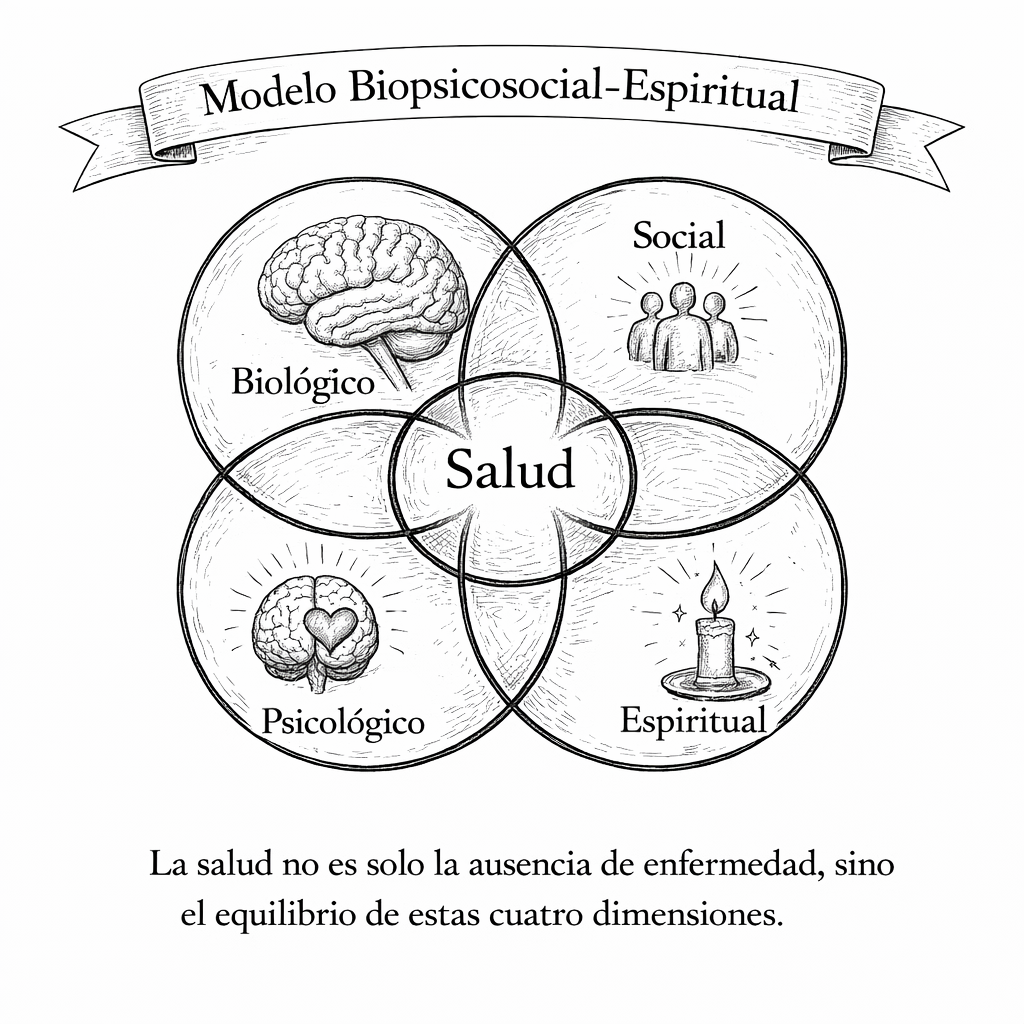
\includegraphics[scale=0.25]{314.png}
		\caption{Modelo bio-psico-social-espiritual}
	\end{figure}
	
	\momento{Fundamento o criterio de discernimiento} 
	El ser humano constituye una unidad inseparable de cuerpo, alma y espíritu. Por lo tanto, la respuesta a los padecimientos no puede ser unilateral, sino que debe ser orgánica e integral, ya que el dolor de quien sufre abarca la totalidad de su vida y sus vínculos.
	
	\momento{Tesis y desarrollo argumental}\\ 
	La aplicación de este modelo integral funciona como un antídoto contra las tentaciones que dividen a la persona. Este enfoque permite superar los cuatro reduccionismos principales:
	
	\begin{enumerate}
		\item Superación del biologicismo: Reconoce que, aunque existe una base neurobiológica real, el hombre no es solo un organismo, sino un espíritu encarnado. La ciencia médica es necesaria pero insuficiente si no atiende la historia y la identidad del sujeto.
		\item Superación del espiritualismo: Evita la idea de que solo rezar basta, ignorando realidades físicas como el síndrome de abstinencia o los daños neurológicos. La espiritualidad actúa en diálogo con las ciencias de la salud, dando sentido a la recuperación.
		\item Superación del individualismo: Entiende que la persona es constitutivamente relacional. La patología a menudo refleja fracturas en los vínculos primarios o en el tejido social, por lo que el cambio requiere de una comunidad de pertenencia.
		\item Superación del colectivismo: Si bien reconoce que los determinantes sociales como la pobreza y la exclusión son fundamentales, el modelo recuerda que la asistencia debe ser individualizada para cada persona concreta.
	\end{enumerate}
	
	\momento{Respuesta a las objeciones}
	\begin{itemize}
		\item \submomento{A la primera:} El cerebro es el órgano afectado, pero la persona es quien padece. Reducir el tratamiento a lo biológico ignora al conductor y su destino; la técnica debe iluminar, pero no nublar la comprensión integral del ser.
		\item \submomento{A la segunda:} La gracia actúa sobre la naturaleza humana. Ignorar los medios médicos o psicológicos bajo un pretexto de fe es una forma de fideísmo que desnaturaliza la misión de curar al hombre en su totalidad.
		\item \submomento{A la tercera:} Ningún sujeto nace determinado, pero la libertad humana está condicionada por traumas o entornos hostiles. El acompañamiento comunitario es lo que permite que esa libertad sea verdaderamente liberada de sus condicionamientos.
	\end{itemize}
	
	\subsection{Artículo 5: Sobre la antropología trinitaria/paulina y la psicología de las emociones}
	
	\momento{Planteo del tema} 
	La comprensión de las emociones en el ámbito de las adicciones suele oscilar entre un determinismo biológico y una visión puramente espiritualista. Sin embargo, para entender el sufrimiento de quien padece un trastorno por uso de sustancias, es necesario recurrir a una visión integral que reconozca la unidad del ser humano. Las emociones y las pasiones no son eventos aislados, sino manifestaciones de una persona que busca, a veces de forma errática, equilibrio y sentido en todas sus dimensiones.
	
	\momento{Pregunta central} 
	¿De qué manera la unidad de cuerpo, alma y espíritu ilumina la comprensión de las emociones y pasiones en la persona con un trastorno por uso de sustancias?.
	
	\momento{Posturas u objeciones existentes}
	\begin{itemize}
		\item \submomento{Objeción 1:} Parece que las emociones y pasiones son fenómenos puramente biológicos, resultado exclusivo de impulsos eléctricos y neurotransmisores, por lo que no requerirían una explicación antropológica o espiritual.
		\item \submomento{Objeción 2:} Parece que las pasiones desordenadas del usuario son exclusivamente problemas del espíritu que deben tratarse solo mediante la vida sacramental, ignorando la estructura psicológica del alma.
	\end{itemize}
	
	\momento{Fundamento o criterio de discernimiento} 
	El ser humano es una unidad inseparable y su antropología es unitaria: un espíritu encarnado donde lo que afecta a una dimensión impacta necesariamente en las demás. Esta estructura permite abordar el dolor emocional sin fragmentar al sujeto.
	
	\momento{Tesis y desarrollo argumental}\\ 
	La antropología trinitaria y paulina ofrece una estructura tridimensional que permite una comprensión profunda de las emociones a través de los siguientes fundamentos:
	
	\begin{enumerate}
		\item La distinción de las facultades: Se reconoce que el alma es el asiento de la vida psicológica donde residen las emociones y los sentimientos. Mientras el espíritu habilita la relación con lo trascendente y el cuerpo la relación con el mundo físico, el alma funciona como el espacio de mediación donde el sufrimiento se procesa y puede convertirse en una fractura interna o trauma.
		\item Relacionalidad trinitaria: Al ser creada a imagen de la Trinidad, la persona es constitutivamente relacional. Las emociones no son estados internos aislados, sino que se gestan en el encuentro con el otro. En la adicción, el desencuentro emocional suele manifestarse como una desconexión de esta esencia relacional.
		\item Unidad sistémica de las pasiones: Debido a la condición de espíritu encarnado, un estímulo biológico como la sustancia inunda los centros de placer del cuerpo, pero impacta directamente en el alma, alterando la capacidad de desear y elegir libremente. Las pasiones son movimientos de una persona integral que busca un sentido de trascendencia.
	\end{enumerate}
	
	\momento{Respuesta a las objeciones}
	\begin{itemize}
		\item \submomento{A la primera:} Aunque las emociones tienen un correlato biológico, este constituye solo la materia de la emoción. Su significado pertenece al alma racional que integra la historia y la identidad del sujeto. Reducirlas a la biología ignora que, aunque el cerebro es el órgano, es la persona quien ama y sufre.
		\item \submomento{A la segunda:} Tratar las adicciones solo como un vacío espiritual ignora que la gracia actúa sobre la naturaleza humana. Para sanar el espíritu, a menudo es indispensable sanar primero las heridas psicológicas del alma, como las emociones traumáticas, y estabilizar el equilibrio del cuerpo. La sanación del Cristo roto debe ocurrir en la totalidad de su unidad trinitaria.
	\end{itemize}
	
	\subsection{Artículo 6: Sobre la naturaleza de la relación entre el sujeto y las sustancias}
	
	\momento{Planteo del tema} 
	El estudio del vínculo entre el individuo y las sustancias psicoactivas (SPA) requiere trascender visiones reduccionistas que equiparan cualquier uso con la patología. Esta interacción no es un evento aislado, sino que se manifiesta como un espectro dinámico de vínculos definidos por la intencionalidad, la frecuencia y el impacto real en la autonomía de la persona. La relación está mediada por una interacción compleja entre la farmacología de la sustancia, la estructura psíquica del individuo y el entorno sociocultural.
	
	\momento{Pregunta central} 
	¿Por qué es fundamental comprender la naturaleza específica del vínculo que una persona establece con las SPA para garantizar un acompañamiento integral y humanizante?.
	
	\momento{Posturas u objeciones existentes}
	\begin{itemize}
		\item \submomento{Objeción 1:} Parece que cualquier contacto con una sustancia psicoactiva debe catalogarse automáticamente como una patología o adicción, independientemente de la intención o el contexto del sujeto.
		\item \submomento{Objeción 2:} Parece que la relación está determinada exclusivamente por la farmacología de la sustancia, asumiendo que el componente químico posee un poder intrínseco que anula de forma inmediata la voluntad de quien la consume.
		\item \submomento{Objeción 3:} Parece que el tipo de relación con el consumo depende únicamente de una decisión moral o de la fuerza de voluntad, ignorando los factores contextuales o el dolor psíquico previo del individuo.
	\end{itemize}
	
	\momento{Fundamento o criterio de discernimiento} 
	La interpretación de cualquier episodio de consumo requiere el análisis de la Tríada de Zinberg\marginnote{Cfr. art.~\ref{art:zinberg} (Juzgar, Brevísimo Glosario)}, que establece que la experiencia biopsicosocial está determinada por tres vectores interconectados: el Sujeto, la Sustancia y el Contexto. Sin el análisis de estos tres elementos, cualquier diagnóstico resulta insuficiente y deshumanizante.
	
	\momento{Tesis y desarrollo argumental}\\ 
	Se debe decir que la relación sujeto-sustancia es un fenómeno multicausal donde el consumo suele cumplir una función específica dentro de la organización interna del individuo. Este vínculo se articula bajo los siguientes principios:
	
	\begin{enumerate}
		\item El Continuo del Consumo: La relación no es un estado binario, sino un espectro que incluye el uso instrumental (la sustancia como herramienta para un fin específico), el recreativo o social (bajo control de normas grupales) y el uso nocivo o dependencia, caracterizado por la neuroadaptación y la pérdida de la capacidad de decisión.
		\item La Hipótesis de la Automedicación: La elección de una sustancia suele responder a un intento del sujeto por regular estados afectivos dolorosos o compensar déficits en su estructura psíquica. La droga actúa aquí como un sustituto de funciones psicológicas ausentes.
		\item El Consumo como Marcador de Identidad: El uso de SPA puede integrarse en el habitus del sujeto, funcionando como un símbolo de distinción o de pertenencia grupal. En contextos de alta vulnerabilidad, puede ser incluso una respuesta a la violencia estructural.
		\item Marcos Regulatorios Culturales: La cultura provee un andamiaje de controles sociales a través de rituales y sanciones que dictan la aceptabilidad del consumo. La transición hacia un uso profano-moderno sin estos marcos aumenta significativamente el riesgo de abuso.
	\end{enumerate}
	
	\momento{Respuesta a las objeciones}
	\begin{itemize}
		\item \submomento{A la primera:} Es imperativo distinguir entre el uso y la patología según el impacto en la autonomía. La gravedad no reside en la sustancia por sí misma, sino en el deterioro clínico y social que el vínculo genera en la persona.
		\item \submomento{A la segunda:} Aunque la farmacología es un vector real, la significación del estímulo depende de la historia y el estado emocional del Sujeto y de las normas del Contexto. La sustancia no actúa sobre un organismo pasivo, sino sobre una persona con identidad singular.
		\item \submomento{A la tercera:} El abordaje debe centrarse en fortalecer la estructura psíquica y modificar las variables contextuales. La verdadera recuperación no se basa en la mera prohibición, sino en el fortalecimiento de los lazos culturales y el proyecto de vida integral del individuo.
	\end{itemize}
	
	
	\subsection{Artículo 7: Sobre la importancia de los contextos culturales en el consumo}
	
	\momento{Planteo del tema} 
	El consumo de sustancias psicoactivas (SPA) no ocurre en un vacío aséptico, sino que está profundamente enraizado en un entramado de significaciones sociales y culturales. El entorno, o setting, no es simplemente un espacio físico, sino una red de rituales, normas y valores que condicionan la experiencia del sujeto. Ignorar estas variables conduce a intervenciones descontextualizadas que no logran comprender por qué una práctica de consumo se sostiene o se vuelve problemática en una comunidad específica.
	
	\momento{Pregunta central} 
	¿De qué manera el contexto cultural y social determina la relación de una persona con las sustancias y por qué su análisis es indispensable para un abordaje integral?.
	
	\momento{Posturas u objeciones existentes}
	\begin{itemize}
		\item \submomento{Objeción 1:} Parece que el contexto es un factor secundario, ya que la adicción es fundamentalmente una enfermedad neurobiológica crónica que afecta los circuitos de recompensa independientemente de la cultura del individuo.
		\item \submomento{Objeción 2:} Parece que centrarse en el entorno social es una forma de colectivismo que diluye la responsabilidad individual, ofreciendo al sujeto una excusa basada en sus circunstancias de pobreza o exclusión.
		\item \submomento{Objeción 3:} Se afirma que las estrategias de prevención deben ser universales y estandarizadas, asumiendo que un mismo programa técnico será igual de efectivo en diversos entornos, sea una gran urbe o una comunidad rural.
	\end{itemize}
	
	\momento{Fundamento o criterio de discernimiento} 
	La experiencia de consumo es el resultado de una interacción sistémica entre tres vectores: el Sujeto, la Sustancia y el Contexto. La cultura funciona como un andamiaje de controles sociales que dicta la aceptabilidad o el rechazo de ciertas conductas a través de rituales y sanciones que representan los juicios de valor del grupo.
	
	\momento{Tesis y desarrollo argumental}\\ 
	El análisis del contexto cultural permite comprender que el consumo es un fenómeno situado que requiere una lectura de las siguientes dimensiones:
	
	\begin{enumerate}
		\item Ritualización vs. Uso Profano: Históricamente, las culturas integraron el uso de sustancias en marcos sacramentales que limitaban su abuso. En la modernidad, la transición hacia un uso profano sin marcos regulatorios tradicionales ha aumentado el riesgo de consumos compulsivos.
		\item El Consumo como Marcador de Identidad: El uso de SPA a menudo se integra en el habitus del sujeto, funcionando como un símbolo de distinción o de pertenencia y cohesión grupal. En muchos sectores, consumir constituye un requisito para no quedar excluido del tejido social inmediato.
		\item Respuesta a la Violencia Estructural: En contextos de alta vulnerabilidad, el consumo puede ser una respuesta adaptativa frente a la violencia estructural y la falta de acceso a derechos básicos. La sustancia actúa aquí como un recurso para anestesiar una realidad percibida como intolerable.
		\item Capital Cultural de Recuperación: La eficacia de un proceso de cambio depende de que las opciones de recuperación incorporen los valores, prácticas y la cosmovisión de la comunidad con la que el sujeto se identifica.
	\end{enumerate}
	
	\momento{Respuesta a las objeciones}
	\begin{itemize}
		\item \submomento{A la primera:} Aunque la neurobiología es un vector real, el cerebro procesa la información y otorga significados basándose en la información almacenada en el ambiente. Un entorno que naturaliza el consumo dispara respuestas automáticas que la farmacología por sí sola no puede modificar.
		\item \submomento{A la segunda:} Reconocer los determinantes sociales no anula la libertad, sino que permite entender las presiones que la condicionan. El objetivo es fortalecer los recursos internos del sujeto mientras se modifican las variables ambientales que asfixian su capacidad de elección.
		\item \submomento{A la tercera:} La estandarización ignora la singularidad de los pueblos; los dispositivos más exitosos son aquellos que validan el saber territorial y comunitario, adaptando la técnica profesional a la sabiduría local.
	\end{itemize}
	
	\subsection{Artículo 8: Sobre los elementos a considerar para evaluar un consumo de SPA}
	
	\momento{Planteo del tema} 
	La evaluación de un consumo de sustancias psicoactivas (SPA) debe trascender la mera identificación de la sustancia o la frecuencia de uso para constituirse como una mirada integral sobre la persona. No se trata de un acto estático de etiquetamiento, sino de un proceso dinámico que busca comprender la función específica que el consumo cumple en la economía psíquica y social del individuo. Una evaluación humanizante evita reducir al sujeto a un diagnóstico, reconociendo que el fenómeno del consumo se agrega a una identidad singular y preexistente.
	
	\momento{Pregunta central} 
	¿Qué elementos fundamentales deben integrar una evaluación integral y humanizante del consumo de SPA para trascender el enfoque meramente clínico y punitivo?.
	
	\momento{Posturas u objeciones existentes}
	\begin{itemize}
		\item \submomento{Objeción 1:} Parece que la evaluación debe centrarse exclusivamente en la farmacología de la sustancia (tipo, cantidad y pureza), ya que estos serían los factores objetivos que determinan la gravedad del daño.
		\item \submomento{Objeción 2:} Parece que el único criterio relevante es la distinción binaria entre dependencia y no dependencia, ignorando los riesgos asociados a consumos que no presentan neuroadaptación pero sí un fuerte impacto social o físico.
		\item \submomento{Objeción 3:} Parece que la evaluación es un acto técnico reservado a un experto que observa desde afuera, donde el usuario es un objeto pasivo de estudio y no un protagonista de su propio proceso.
	\end{itemize}
	
	\momento{Fundamento o criterio de discernimiento} 
	La evaluación se fundamenta en el análisis de la Tríada de Zinberg, la cual establece que la experiencia de consumo es el resultado de la interacción entre el Sujeto, la Sustancia y el Contexto. Este criterio sistémico, enmarcado en el modelo biopsicosocial-espiritual, impide interpretaciones aisladas de la droga y obliga a considerar la historia vital y el entorno como componentes inseparables del fenómeno.
	
	\momento{Tesis y desarrollo argumental}\\ 
	Una evaluación completa de la relación sujeto-sustancia debe considerar los siguientes pilares fundamentales:
	
	\begin{enumerate}
		\item Análisis funcional e intencionalidad: Es preciso identificar si el consumo tiene un carácter experimental, recreativo, instrumental o si responde a una hipótesis de automedicación. En este último caso, el consumo funciona como un síntoma de una fractura interna o trauma previo que la persona intenta anestesiar.
		\item Ubicación en el continuo del consumo: Se debe determinar en qué punto del espectro se encuentra el vínculo, evaluando el grado en que la autonomía y la capacidad de decisión se han visto deterioradas por la neuroadaptación.
		\item Estado de las redes de memoria: Evaluar si el consumo está gatillado por redes de memoria desadaptativas que almacenan vivencias traumáticas. Esto permite entender el consumo como una respuesta automática ante un entorno percibido como hostil o intolerable.
		\item Identificación del capital de recuperación: La evaluación no solo mira el déficit, sino los recursos disponibles: capital personal (salud, habilidades), familiar/social (redes de apoyo) y comunitario/cultural (sentido de pertenencia).
		\item Significación cultural del acto: Analizar si el consumo está mediado por rituales comunitarios o si ha pasado a ser un uso profano-moderno y solitario, donde la pérdida del marco regulador social aumenta la vulnerabilidad.
	\end{enumerate}
	
	\momento{Respuesta a las objeciones}
	\begin{itemize}
		\item \submomento{A la primera:} Aunque la sustancia es un vector real, su efecto depende de cómo el Sujeto significa el estímulo según su historia. Centrarse solo en la química es un reduccionismo que ignora que el cerebro es el órgano, pero la persona es quien ama y sufre.
		\item \submomento{A la segunda:} La evaluación debe contemplar el uso nocivo incluso antes de que exista una dependencia clínica. Ignorar los riesgos de consumos desregulados impide una prevención efectiva y el fortalecimiento de la autoeficacia.
		\item \submomento{A la tercera:} El acompañamiento eficaz debe basarse en la escucha activa y la hospitalidad, reconociendo que la persona es experta en su propia vida. Una evaluación que no valide la palabra del sujeto bloquea la recuperación al generar un rechazo hacia sí mismo.
	\end{itemize}
	
	\newpage
	
	\section{Trauma, Estructuras de Personalidad y Patología Dual}
	
	Esta sección aborda la profunda relación entre la historia traumática del individuo y el desarrollo de conductas adictivas, entendiendo que el consumo de sustancias funciona frecuentemente como un intento autoterapéutico para anestesiar un dolor derivado de una fractura interna o un desamparo temprano. Se profundiza en la distinción clínica entre las estructuras de personalidad psicótica, neurótica y limítrofe (borderline), analizando cómo el grado de consolidación del sujeto y la robustez de sus redes de memoria determinan su capacidad para procesar la realidad sin recurrir a mecanismos de evasión o desconexión. El núcleo del análisis reside en la patología dual\label{art:dual}\index{patología dual|textbf}, definida como la coexistencia de trastornos mentales de base con el uso problemático de sustancias, lo cual exige un abordaje especializado que no se limite a tratar los síntomas de consumo, sino que procure la sanación de los traumas profundos y la estabilización del sistema nervioso desregulado. Finalmente, se propone un modelo de intervención que trasciende lo meramente patologizante, centrando la respuesta en el establecimiento de una comunidad de apego seguro y una cultura terapéutica que permita la integración gradual de la personalidad y la restauración de la dignidad de la persona.
	
	\subsection{Artículo 1: Sobre la naturaleza manifiesta del problema de las adicciones}
	
	\momento{Planteo del tema} 
	La problemática del consumo de sustancias se presenta en la actualidad como una realidad innegable que genera un inmenso sufrimiento en individuos, familias y comunidades. Lejos de ser un fenómeno aislado o estático, se manifiesta como una crisis que atraviesa todas las capas de la sociedad, exigiendo una mirada que no se quede en la superficie de la sustancia, sino que reconozca el dolor humano que subyace al consumo. La Iglesia y las organizaciones sociales se enfrentan al desafío de responder ante un flagelo que actúa de forma expansiva y desoladora.
	
	\momento{Pregunta central} 
	¿Es el consumo de sustancias un problema manifiesto que requiere una respuesta urgente e integral por parte de la Iglesia y la sociedad?.
	
	\momento{Posturas u objeciones existentes}
	\begin{itemize}
		\item \submomento{Objeción 1:} Parece que el problema no es tan grave o manifiesto, debido a que muchos tipos de consumo están naturalizados socialmente y se consideran parte de la cultura del bienestar o la recreación.
		\item \submomento{Objeción 2:} Parece que la adicción es un problema que solo atañe a los sectores más vulnerables o desposeídos, por lo que no constituiría un desafío universal para toda la comunidad eclesial.
		\item \submomento{Objeción 3:} Se afirma que el verdadero problema es el narcotráfico y que, por tanto, la solución debe ser estrictamente legal y policial, dejando en un segundo plano la intervención pastoral o educativa.
	\end{itemize}
	
	\begin{figure}[h!]
		\centering
		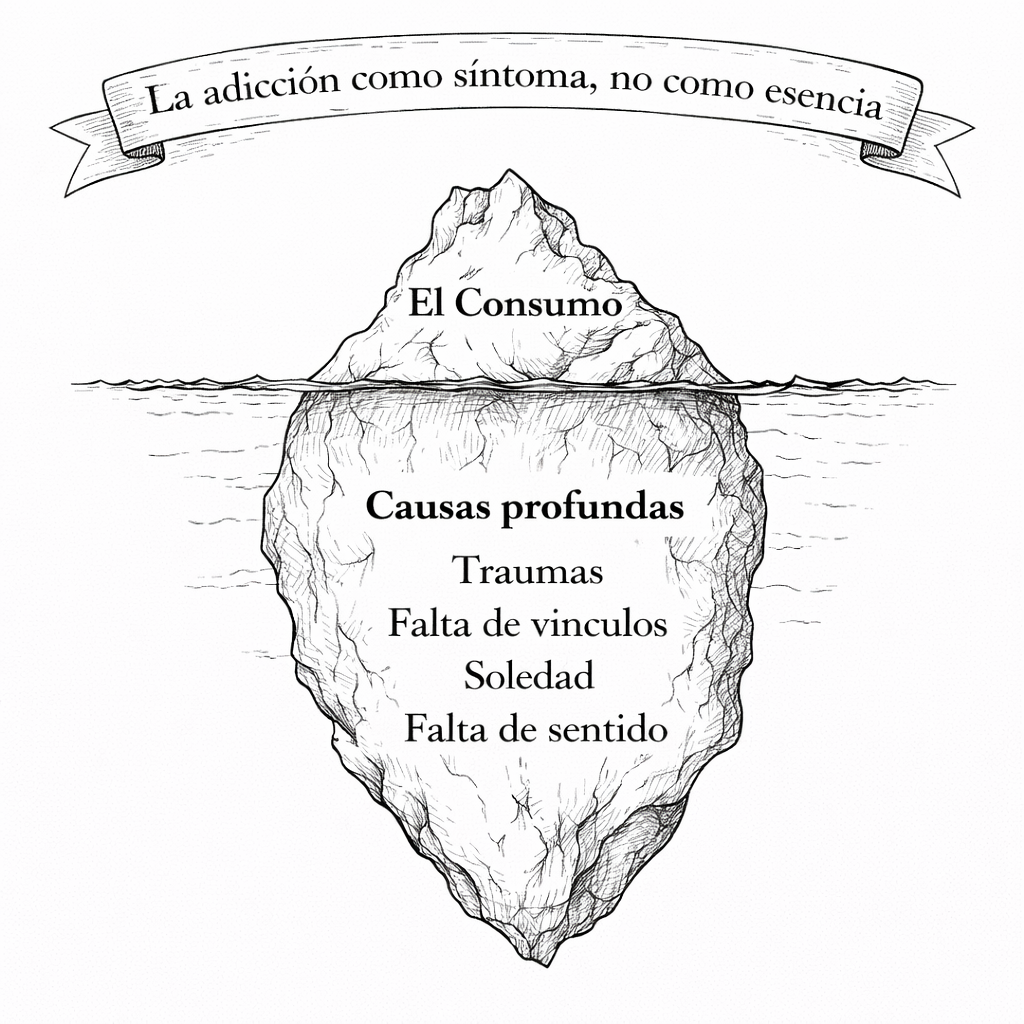
\includegraphics[scale=0.25]{321.png}
		\caption{El consumo como síntoma}
	\end{figure}
	
	\momento{Fundamento o criterio de discernimiento} 
	El problema de las adicciones es comparable a una mancha de aceite que lo invade todo, sin reconocer fronteras geográficas ni humanas. Ataca por igual a todos los sectores sociales, lo que impide que la comunidad permanezca indiferente ante una realidad que compromete la integridad de la persona y la vida de los más jóvenes.
	
	\momento{Tesis y desarrollo argumental}\\ 
	La problemática de los trastornos por uso de sustancias es una realidad creciente y multicausal que requiere una respuesta inmediata basada en los siguientes puntos:
	
	\begin{enumerate}
		\item Crecimiento global y nuevas sustancias: El fenómeno se expande con la aparición anual de cientos de nuevas sustancias psicoactivas, cuyos efectos suelen ser desconocidos para el consumidor, aumentando el riesgo de daños irreversibles.
		\item Impacto en la salud integral: El consumo contribuye significativamente a la carga global de enfermedades y mortalidad prematura. No se trata solo de la dependencia, sino de ser un vector de transmisión para patologías severas y un factor de deterioro físico y mental crónico.
		\item Crisis de personas antes que de sustancias: Más allá de la composición química de la droga, el problema manifiesto reside en personas desoladas por la exclusión, la falta de sentido o el dolor profundo. El sujeto recurre a la sustancia como un medio para escapar de una realidad desesperanzadora.
		\item Costo social y cultura de la muerte: El fenómeno genera una forma de dependencia que reduce la productividad y la alegría de vivir, imponiendo una lógica de descarte que afecta especialmente a la juventud.
	\end{enumerate}
	
	\momento{Respuesta a las objeciones}
	\begin{itemize}
		\item \submomento{A la primera:} La naturalización de sustancias legales o funcionales es un síntoma de una sociedad que a menudo niega la enfermedad hasta que el deterioro es absoluto. El bienestar aparente oculta una dependencia que erosiona la libertad del individuo.
		\item \submomento{A la segunda:} Aunque los sectores con menos recursos sufren más por la falta de redes de apoyo, la adicción es una pandemia transversal que golpea a todas las clases sociales sin distinción.
		\item \submomento{A la tercera:} El enfoque punitivo centrado solo en la oferta ha demostrado ser insuficiente. El problema real se manifiesta en la demanda, la cual solo puede ser abordada mediante la prevención, la educación en valores y el acompañamiento humano de la persona en su singularidad.
	\end{itemize}
	
	\subsection{Artículo 2: Sobre la distinción clínica de las estructuras de personalidad y la patología dual}
	
	\momento{Planteo del tema} 
	Para un abordaje profundo del sufrimiento humano, no basta con observar la conducta de consumo; es imperativo comprender sobre qué cimiento psíquico se apoya dicha conducta. La distinción entre las diferentes estructuras de personalidad, tal como la propone la tradición psicodinámica estructural, permite identificar el grado de fragilidad o solidez con que un sujeto procesa su realidad y sus vínculos. Entender la adicción como un síntoma de una organización mental previa ayuda a diseñar estrategias de acompañamiento que no solo busquen la abstinencia, sino la integración de una personalidad que se encuentra fracturada.
	
	\momento{Pregunta central} 
	¿Existe una distinción clínica clara entre las estructuras psicótica, neurótica y limítrofe, y de qué manera condicionan la aparición de la patología dual\marginnote{Cfr. art.~\ref{art:dual} (Juzgar, La psiquis, Trauma...)}?.
	
	\momento{Posturas u objeciones existentes}
	\begin{itemize}
		\item \submomento{Objeción 1:} Parece que no es necesario realizar distinciones clínicas entre estructuras de personalidad, ya que el trastorno por uso de sustancias debe ser tratado como una condición uniforme que afecta los circuitos de recompensa del cerebro por igual en todos los sujetos.
		\item \submomento{Objeción 2:} Parece que centrarse en diagnósticos de base desvía la atención del problema principal, que es la voluntad del individuo para abandonar el consumo y su compromiso con un camino moral o espiritual.
	\end{itemize}
	
	\momento{Fundamento o criterio de discernimiento} 
	
	\marginnote{Cfr. La patología dual (cap. 9, dimensión biológica)}
	
	El grado de constitución subjetiva y el desarrollo de la personalidad son criterios fundamentales para entender que la adicción no es el problema en sí mismo, sino el síntoma de una fractura interna. La intervención debe ser proporcional a la fragilidad de la estructura sobre la que se monta el consumo.
	
	\momento{Tesis y desarrollo argumental}\\ 
	Se debe decir que la distinción entre las estructuras de personalidad depende del nivel de consolidación que el sujeto alcanzó frente a sus vivencias y su entorno primario. Se distinguen tres grandes organizaciones:
	
	\begin{enumerate}
		\item \textbf{Estructura psicótica:} Es la más frágil, originada frecuentemente en medios hostiles o vínculos primarios deficientes que impidieron la integración de redes de memoria adaptativas. Ante crisis, estos sujetos utilizan mecanismos de disociación y desconexión, lo que produce una alteración del juicio de realidad y la aparición de alucinaciones o delirios.
		\item \textbf{Estructura neurótica:} Presenta una mayor solidez, habiendo contado habitualmente con vínculos primarios suficientemente buenos que instalaron sensaciones de calma. Su juicio de realidad se mantiene conservado y sus mecanismos defensivos no los apartan completamente del mundo circundante.
		\item \textbf{Estructura limítrofe (borderline):} Se ubica en la frontera entre las anteriores. Se caracteriza por una notoria impulsividad y pérdida de contacto con la realidad en momentos de descompensación, sin llegar a la fragmentación psicótica total pero sin alcanzar la integración neurótica.
	\end{enumerate}
	
	\begin{itemize}
		\item \textbf{Advertencia:} Esta distinción en tres organizaciones proviene del modelo psicodinámico estructural, una tradición clínica de amplia difusión en América Latina que ha demostrado particular utilidad para comprender la relación entre la fragilidad de la personalidad y la vulnerabilidad al consumo. Es necesario señalar que otros marcos clasificatorios organizan los trastornos de personalidad de manera diferente. El DSM-5\label{ds5} utiliza un sistema de categorías diagnósticas discretas (trastorno límite, trastorno antisocial, etc.) que no se ordena según niveles de integración estructural. La CIE-11\label{cie}, vigente desde 2022, ha adoptado un modelo dimensional que evalúa la severidad del trastorno de personalidad en un continuo (leve, moderado, grave) junto con rasgos predominantes, alejándose significativamente del enfoque categorial. Este manual opta por la perspectiva estructural porque permite al acompañante captar con rapidez el grado de fragilidad del hermano que tiene delante y ajustar la intensidad y el tipo de sostén que ofrece, lo cual resulta operativamente más útil en el territorio que una clasificación por categorías diagnósticas aisladas. No obstante, los equipos que trabajen con profesionales formados en otros marcos encontrarán que las tres organizaciones aquí descritas pueden dialogar con esos sistemas sin contradicción: lo que el modelo estructural llama fragilidad psicótica corresponde, en términos generales, a los niveles de severidad grave de la CIE-11; la estructura neurótica a los niveles leves; y la limítrofe a los moderados.
	\end{itemize}
	
	La patología dual\index{patología dual!función de la sustancia|textbf} es la coexistencia de este cuadro de base con un consumo problemático. En estas situaciones, la sustancia cumple una función de supervivencia psíquica, actuando como un anestésico frente a una vida percibida como amenaza constante debido a traumas no procesados.
	
	\begin{alertaPastoral}
		En los cuadros de patología dual\index{patología dual!y medicación psiquiátrica}, la intervención psiquiátrica y la medicación adecuada constituyen frecuentemente una condición necesaria para que el proceso de acompañamiento pueda sostenerse. Una persona con una estructura psicótica descompensada o con un episodio depresivo severo no puede participar de un grupo terapéutico, elaborar su historia en un espacio de escucha ni sostener una experiencia espiritual si su sistema nervioso no ha alcanzado un umbral mínimo de estabilización. La medicación psiquiátrica prescrita y supervisada por un profesional no es una contradicción con el modelo integral que este manual propone; es parte de él. Así como el artículo 8.1.4 advierte que tratar las adicciones solo con oración ignorando la biología es una forma de espiritualismo reductor, es igualmente necesario advertir que rechazar la medicación legítima bajo el argumento de que «se reemplaza una droga con otra» es una forma de ignorancia que puede costar vidas. La medicación no sana por sí sola — el manual ha sido claro en que el vínculo, la comunidad y el sentido son indispensables —, pero en muchos casos crea las condiciones biológicas mínimas para que la persona pueda estar disponible para el encuentro sanador que la comunidad le ofrece. Los equipos pastorales que acompañan a personas con patología dual deben articularse con los servicios de salud mental del territorio para garantizar que la dimensión farmacológica del tratamiento no quede desatendida por falta de acceso, por estigma institucional o por una concepción errada de lo que significa una recuperación integral.
	\end{alertaPastoral}
	
	\momento{Respuesta a las objeciones}
	\begin{itemize}
		\item \submomento{A la primera:} Aunque la neurobiología es real, un abordaje que solo mire la sustancia es ineficiente. La recuperación estable depende de sanar la interioridad no integrada y compensar el cuadro de base que motiva la conducta de fuga.
		\item \submomento{A la segunda:} La adicción no es una mera cuestión de voluntad. En las estructuras más frágiles, el consumo es una herramienta de supervivencia frente al dolor insoportable. Por ello, la respuesta debe ser una cultura terapéutica que ofrezca un apego seguro para que la personalidad pueda alcanzar un mayor grado de integración.
	\end{itemize}
	
	\subsection{Artículo 3: Sobre la implementación del Tratamiento Informado en el Trauma}
	
	\momento{Planteo del tema} 
	La gran mayoría de las personas que presentan trastornos por uso de sustancias han atravesado historias de trauma complejo, negligencia o abusos en la infancia que han marcado sus redes de memoria desadaptativas. Un tratamiento informado en el trauma propone un cambio de paradigma: no se busca únicamente tratar la conducta adictiva superficial, sino abordar y sanar la herida subjetiva que la sustenta, entendiendo que el consumo es el lenguaje de un dolor que no ha podido ser nombrado de otra manera.
	
	\momento{Pregunta central} 
	¿Cómo debe implementarse un Tratamiento Informado en el Trauma, reconociendo que el dolor emocional suele preceder a la adicción?.
	
	\momento{Posturas u objeciones existentes}
	\begin{itemize}
		\item \submomento{Objeción 1:} Parece que el tratamiento debe centrarse exclusivamente en la abstinencia y en la reparación neurobiológica del cerebro, considerando que indagar en el pasado o en dolores emocionales es secundario frente a la urgencia de detener el consumo.
		\item \submomento{Objeción 2:} Parece que centrarse en el trauma podría victimizar al sujeto, restándole responsabilidad individual sobre su proceso de cambio y permitiéndole justificar su conducta presente como una consecuencia inevitable del dolor previo.
	\end{itemize}
	
	\momento{Fundamento o criterio de discernimiento} 
	
	\marginnote{Cfr. La restauración de la imagen de Dios tras el trauma (cap. 7)}
	
	La adicción es frecuentemente un síntoma de una fractura interna o un intento autoterapéutico de aliviar una vida que se ha vuelto intolerable debido a vivencias traumáticas. Por lo tanto, cualquier abordaje que ignore el malestar primario que precede al consumo será ineficiente para lograr una sanación integral.
	
	\momento{Tesis y desarrollo argumental}\\ 
	Se debe decir que un Tratamiento Informado en el Trauma no busca solo tratar la conducta, sino sanar la herida que la sostiene. Este enfoque reconoce que la recuperación real ocurre cuando se estabiliza el sistema nervioso desregulado y se procesa el sufrimiento acumulado. La implementación de este modelo se basa en los siguientes pilares:
	
	\begin{enumerate}
		\item Prioridad de la seguridad: El tratamiento debe garantizar un entorno física y emocionalmente seguro para evitar la revictimización. Todo el equipo debe estar capacitado para identificar disparadores o señales de alerta emocional que activen redes de memoria negativas.
		\item Sensibilidad y ternura: Es necesario abandonar el lenguaje moralizante por uno de cercanía y hospitalidad. El acompañamiento debe ser una humanización del recorrido donde la escucha sea el primer paso para que el sujeto pueda simbolizar su dolor.
		\item Enfoque en la resiliencia: En lugar de centrarse solo en el déficit o en lo que la persona ha perdido, se trabaja sobre el capital de recuperación, identificando las fortalezas y recursos que el sujeto posee para reconstruir su proyecto de vida.
		\item Integración interdisciplinaria: Se requiere coordinar la atención médica, psicológica y espiritual para abordar la grieta existencial donde se instaló la adicción. El vínculo comunitario es el factor que verdaderamente permite integrar la personalidad fracturada.
	\end{enumerate}
	
	\momento{Respuesta a las objeciones}
	\begin{itemize}
		\item \submomento{A la primera:} Aunque la desintoxicación es necesaria, la ciencia demuestra que el estrés crónico por trauma altera los circuitos cerebrales de recompensa. Si no se trata el malestar primario, el cerebro seguirá buscando la sustancia como la única vía conocida de escape y alivio.
		\item \submomento{A la segunda:} El enfoque en el trauma no anula la responsabilidad, sino que la empodera. Al comprender que su consumo fue un mecanismo de supervivencia fallido, la persona puede dejar de identificarse con el estigma y empezar a verse como un sujeto digno capaz de elegir un futuro diferente.
	\end{itemize}
	
	
	\newpage
	
	\section{El Proceso de Cambio y la Dinámica Motivacional}
	
	Esta sección aborda la recuperación como un proceso dinámico de crecimiento continuo, en el cual el objetivo trasciende la mera abstinencia\index{abstinencia!y proceso de cambio} para centrarse en la mejora del funcionamiento integral y la búsqueda del máximo potencial de la persona. A través del Modelo Transteórico del Cambio, se comprende que la motivación no es un rasgo estático, sino un estado intencional y cambiante que fluye bajo influencias internas y externas, atravesando etapas específicas: precontemplación, contemplación, preparación, acción, mantenimiento y finalización. Este enfoque permite reconocer que el camino hacia la sanación no es lineal, integrando la recaída no como un fracaso definitivo, sino como una oportunidad de aprendizaje y reentrada al ciclo de cambio. Finalmente, se destaca la importancia de identificar y fortalecer el capital de recuperación\index{capital de recuperación} —el conjunto de recursos personales, familiares, sociales y culturales— como el sustento necesario para que el individuo asuma con autonomía un proyecto de vida pleno, digno y sostenible.
	
	\subsection{Artículo 1: Sobre las etapas del proceso de cambio y sus necesidades}
	
	\momento{Planteo del tema} 
	La recuperación en las adicciones no debe entenderse como un suceso repentino basado únicamente en un acto de voluntad, sino como un proceso de crecimiento continuo y dinámico. La motivación para el cambio no es un rasgo de personalidad fijo, sino un estado intencional que fluctúa. Por ello, es necesario contar con un mapa que permita identificar en qué momento subjetivo se encuentra la persona para ofrecer el apoyo adecuado a sus necesidades específicas. Entre los diversos marcos propuestos por la psicología para comprender este proceso, el Modelo Transteórico del Cambio constituye una de las herramientas más influyentes y extendidas en el campo de las adicciones. Este manual lo adopta como referencia organizativa principal, reconociendo tanto su valor pedagógico como las limitaciones que la investigación posterior ha señalado.
	
	\momento{Pregunta central} 
	¿Es el proceso de cambio en las adicciones un camino lineal y estático, o se compone de etapas dinámicas con necesidades de apoyo específicas?.
	
	\momento{Posturas u objeciones existentes}
	\begin{itemize}
		\item \submomento{Objeción 1:} Parece que la motivación para el cambio es estática. Bajo esta visión, una persona posee o no posee motivación, y si no la tiene, el acompañante no puede influir en su decisión, siendo la falta de voluntad responsabilidad exclusiva del individuo.
		\item \submomento{Objeción 2:} Parece que la recaída es un fracaso definitivo. Según esta lógica, si una persona vuelve a consumir, ha perdido todo el progreso previo y debe ser considerada como alguien que abandonó su compromiso con el cambio.
		\item \submomento{Objeción 3:} Parece que el proceso de cambio se ajusta siempre a una secuencia de etapas ordenadas y previsibles, lo que sugeriría que toda recuperación sigue un itinerario lineal desde la precontemplación hasta la finalización, y que quienes no transitan esas etapas en el orden previsto estarían fuera del modelo.
	\end{itemize}
	
	\momento{Fundamento o criterio de discernimiento} 
	El cambio es un proceso dinámico en el cual las personas atraviesan etapas previsibles a ritmos diferentes, moviéndose hacia adelante y hacia atrás según su nivel de motivación intencional. La intervención debe ser artesanal y ajustada al momento que atraviesa el sujeto.
	
	\momento{Tesis y desarrollo argumental}\\ 
	La recuperación es un ciclo de aprendizaje donde el Modelo Transteórico identifica seis etapas con características y necesidades de apoyo particulares:
	
	\begin{enumerate}
		\item \textbf{Precontemplación}: El individuo no tiene intención de cambiar y a menudo subestima el problema. La necesidad de apoyo radica en generar confianza y aumentar la toma de conciencia sobre los riesgos sin ejercer presión.
		\item \textbf{Contemplación}: La persona reconoce el problema pero experimenta ambivalencia. Requiere ayuda para resolver esa dualidad entre querer y no querer cambiar, fortaleciendo la confianza en su capacidad de lograrlo.
		\item \textbf{Preparación}: Existe la intención de actuar pronto y se han dado pasos pequeños. El apoyo debe centrarse en elegir estrategias de cambio apropiadas y negociar un plan concreto.
		\item \textbf{Acción}: El sujeto modifica activamente su comportamiento. Es el momento de mayor riesgo, donde se necesita afirmación constante de los logros y aprendizaje de habilidades para manejar la abstinencia.
		\item \textbf{Mantenimiento}: Se consolidan los logros para evitar la recurrencia. El apoyo se orienta a desarrollar nuevos estilos de vida, amistades sanas y metas que sustituyan el rol de la sustancia.
		\item \textbf{Finalización o terminación}: El cambio se ha integrado totalmente por más de dos años y la tentación ha desaparecido. La persona ya no actúa por vigilancia, sino desde una libertad recuperada.
	\end{enumerate}
	\begin{itemize}
		\item \textbf{Alcances y limitaciones del modelo.} El Modelo Transteórico fue desarrollado originalmente para el estudio del abandono del tabaquismo, y su generalización a otras sustancias y a las adicciones conductuales ha sido objeto de discusión en la literatura científica. Revisiones posteriores han cuestionado que las etapas sean tan discretas y secuenciales como el modelo original propone; la experiencia clínica y territorial confirma que muchas personas oscilan entre etapas, las saltean o las transitan de forma simultánea. Asimismo, el modelo no integra adecuadamente la dimensión del cambio abrupto o conversivo —lo que algunos autores denominan cambio cuántico (\textit{quantum change})—, en el cual una experiencia intensa (un encuentro, una crisis, un acontecimiento espiritual) precipita una transformación profunda que no sigue la lógica gradual de las etapas. Esta dimensión es particularmente relevante para una pastoral que reconoce la posibilidad de la conversión y del encuentro transformador con Cristo como motor de cambio radical. El modelo se ofrece, por tanto, como una herramienta de orientación que ayuda al acompañante a situar al hermano en su proceso, pero no como un itinerario obligatorio ni como la única forma legítima de comprender la recuperación.	
	\end{itemize}
	
	
	\momento{Respuesta a las objeciones}
	\begin{itemize}
		\item \submomento{A la primera:} La motivación es dinámica y con propósito. El rol del acompañante no es pasivo; su tarea es ayudar al usuario a entender sus propias dudas y metas para inclinar la balanza hacia el cambio.
		\item \submomento{A la segunda:} La recaída o recurrencia es un acontecimiento que dispara un nuevo ciclo y debe verse como una oportunidad de aprendizaje pedagógico. Quien recae necesita una evaluación para reanudar el proceso y reparar la confianza en sí mismo, no una condena que lo excluya.
		\item \submomento{A la tercera:} El modelo es un mapa, no el territorio. La realidad del cambio humano es más fluida y menos predecible que cualquier esquema de etapas. La experiencia pastoral demuestra que algunos hermanos transitan las etapas de forma no lineal, que otros experimentan transformaciones abruptas que no encajan en la secuencia prevista, y que la singularidad de cada proceso de vida excede toda clasificación. El valor del modelo reside en ofrecer al acompañante un lenguaje compartido para identificar necesidades y ajustar su respuesta, no en prescribir un camino único.
	\end{itemize}
	
	\subsection{Artículo 2: Sobre la etapa de finalización o terminación}
	
	\momento{Planteo del tema} 
	En los modelos de tratamiento de las adicciones, suele omitirse el horizonte de llegada, manteniendo al sujeto en un estado de alerta permanente. Sin embargo, para una antropología que busca el máximo potencial de la persona, es indispensable definir un estado de integración total donde el cambio deja de ser un esfuerzo consciente para convertirse en una nueva naturaleza. La etapa de finalización representa la culminación del proceso donde la libertad se recupera plenamente y el individuo trasciende su identidad previa de paciente.
	
	\momento{Pregunta central} 
	¿Es necesario incluir la etapa de finalización o terminación tras el mantenimiento, y cómo se define este estado de integración del cambio?.
	
	\momento{Posturas u objeciones existentes}
	\begin{itemize}
		\item \submomento{Objeción 1:} Parece que no es necesario incluir una etapa de finalización, dado que los trastornos por uso de sustancias se definen como una enfermedad crónica y recurrente, lo que obligaría al individuo a permanecer en un estado de vigilancia perpetua durante toda su vida.
		\item \submomento{Objeción 2:} Parece que la etapa de mantenimiento es suficiente, ya que consiste en consolidar los logros y prevenir recaídas de forma continua; añadir una etapa de terminación resulta redundante y podría generar una falsa sensación de seguridad en el usuario.
		\item \submomento{Objeción 3:} Se afirma que la recuperación es un proceso de gestión a lo largo de toda la vida, por lo que establecer un punto final contradice la naturaleza del crecimiento humano continuo y el dinamismo de la psiquis.
	\end{itemize}
	
	\momento{Fundamento o criterio de discernimiento} 
	Es fundamental contemplar la etapa de finalización para validar la capacidad del ser humano de trascender el trastorno y alcanzar una vida autodirigida. En esta fase, el cambio se ha integrado de tal modo que la tentación de volver al comportamiento anterior ha perdido su poder de determinación sobre la conducta del sujeto, coexistiendo con una libertad recuperada y una vigilancia serena que no angustia sino que protege, permitiendo que la persona deje de ser un destinatario de servicios para ser un protagonista pleno en su comunidad.
	
	\momento{Tesis y desarrollo argumental}\\ 
	La inclusión de la etapa de terminación es necesaria para dar cuenta de la plenitud del desarrollo humano y se fundamenta en los siguientes puntos:
	
	\begin{enumerate}
		\item Validación del éxito terapéutico: Evita que la persona quede atrapada en una identidad eterna de enfermo o persona dependiente, lo cual contradice el objetivo de alcanzar el máximo potencial y reconocer que la dignidad ontológica es superior a cualquier patología.
		\item Diferenciación de la lucha: Mientras el mantenimiento requiere un esfuerzo consciente y una vigilancia continua contra situaciones de riesgo, la finalización marca el paso hacia un estado donde la libertad ya no se experimenta como una lucha constante contra el impulso, sino como una disposición estable del corazón que, sin negar la fragilidad constitutiva de la condición humana, permite al sujeto habitar su vida desde el proyecto y no desde la urgencia. El comportamiento saludable ya no es una imposición externa o un autocontrol tenso, sino una elección natural.
		\item Criterios de integración total: Se define por una temporalidad de al menos dos años de comportamiento saludable ininterrumpido, la ausencia total de ambivalencia frente al consumo y una autoeficacia plena. El sujeto ya no consume para aliviar el malestar, sino que ha construido un estilo de vida con propósito que sustituye la dinámica del consumo.
	\end{enumerate}
	
	\momento{Respuesta a las objeciones}
	\begin{itemize}
		\item \submomento{A la primera:} Aunque la neuroadaptación sea un dato biológico persistente, las dimensiones espiritual y psicológica permiten a la persona reemplazar los hábitos aprendidos por nuevos repertorios saludables que se vuelven espontáneos. La terminación celebra la libertad recuperada frente a la historia clínica.
		\item \submomento{A la segunda:} La redundancia es aparente. El mantenimiento es un estado de alerta ante el riesgo, mientras que la terminación es el estado donde el plan de recuperación ha evolucionado hacia un sentido de vida trascendente en el que la droga ya no es una opción de respuesta al estrés o al dolor.
		\item \submomento{A la tercera:} Si bien el crecimiento humano es perpetuo, el cambio específico respecto a la conducta adictiva sí tiene un punto de resolución satisfactorio. El objetivo del acompañamiento es que el individuo recupere su autonomía total y se reintegre como un miembro activo y sano de la familia humana.
	\end{itemize}
	
	\subsection[Artículo 3: Sobre la motivación para el cambio]{Artículo 3: Sobre la naturaleza de la motivación para el cambio}
	
	
	\momento{Planteo del tema} 
	La motivación es el motor fundamental del proceso de recuperación, pero a menudo se malentiende como un recurso que el individuo posee o no de forma permanente. Para un acompañamiento eficaz, es necesario comprender que la voluntad de cambio no es un rasgo de personalidad estático, sino una fuerza viva que fluctúa y se ve influenciada por la interacción entre el mundo interno del sujeto y su entorno social.
	
	\momento{Pregunta central} 
	¿Se diferencia la motivación para el cambio por ser un estado estático o, por el contrario, es un proceso dinámico e intencional influenciado por diversos factores?.
	
	\momento{Posturas u objeciones existentes}
	\begin{itemize}
		\item \submomento{Objeción 1:} Parece que la motivación es estática, entendiéndose como un rasgo de personalidad. Bajo esta visión, si un usuario no está motivado, el acompañante tiene pocas posibilidades de influir y la falta de avance es responsabilidad exclusiva del individuo.
		\item \submomento{Objeción 2:} Parece que la motivación es unilateral, centrada únicamente en el deseo de dejar la sustancia. Por tanto, si una persona continúa consumiendo, se asume que no existe motivación alguna para el cambio.
		\item \submomento{Objeción 3:} Se afirma que si la adicción afecta los centros de placer, la motivación sería un simple reflejo bioquímico y no un proceso intencional o psicológico.
	\end{itemize}
	
	\momento{Fundamento o criterio de discernimiento} 
	La motivación no es un rasgo fijo, sino un estado dinámico que puede fluctuar a lo largo del tiempo y según las situaciones. Se mueve entre metas contradictorias y varía en intensidad conforme la persona resuelve sus dudas y ambivalencias.
	
	\momento{Tesis y desarrollo argumental}\\ 
	Se debe decir que la motivación es un proceso dinámico, intencional y cambiante. Reconoce que el individuo puede oscilar entre el deseo de recuperarse y el impulso de consumir, viéndose afectado por dos grupos de influencias:
	
	\begin{enumerate}
		\item Influencias internas: Incluyen los estados emocionales (donde la esperanza aumenta la motivación), las metas de vida (el deseo de trabajar o formar una familia) y las percepciones cognitivas sobre los riesgos y beneficios de la conducta actual.
		\item Influencias externas: Se refieren a los vínculos sociales (familia y amigos que apoyan o minan el esfuerzo), eventos críticos (como un arresto o el nacimiento de un hijo) y el apoyo comunitario que ofrece recursos para sostener la decisión.
		\item La resolución de la ambivalencia: La motivación dinámica entiende que es normal sentir  dos personalidades  en conflicto. El proceso de cambio avanza a medida que el sujeto logra inclinar la balanza hacia sus valores de vida superiores.
	\end{enumerate}
	
	\momento{Respuesta a las objeciones}
	\begin{itemize}
		\item \submomento{A la primera:} Al entender la motivación como algo dinámico, el rol del acompañante deja de ser pasivo. Su tarea consiste en ayudar a la persona a resolver su ambivalencia, facilitando que el deseo de cambio positivo prevalezca mediante la escucha activa.
		\item \submomento{A la segunda:} La motivación puede variar drásticamente entre diferentes conductas. Un usuario puede estar muy motivado para mejorar su salud física pero tener una motivación baja para abandonar un consumo específico; el acompañamiento debe respetar esta singularidad para trabajar sobre lo que el sujeto sí está dispuesto a cambiar.
		\item \submomento{A la tercera:} Aunque los procesos biológicos condicionan la conducta, el ser humano posee una dimensión espiritual y volitiva que le permite trascender sus impulsos. El tratamiento busca fortalecer el proyecto de vida para que la parte racional retome el mando sobre la urgencia del consumo.
	\end{itemize}
	
	\subsection{Artículo 4: Sobre la naturaleza de la recaída y su valor pedagógico}
	
	\marginnote{Lc 22, 31-34.61-62\label{lc22.31} — \textit{Yo he rogado por ti, para que tu fe no desfallezca. Y tú, cuando hayas vuelto, confirma a tus hermanos... Y, saliendo afuera, lloró amargamente}}
	
	\momento{Planteo del tema} 
	En el abordaje de las adicciones, la ruptura de la abstinencia suele ser interpretada bajo una lógica de fracaso o culpa moral. Sin embargo, para una mirada integral, es necesario comprender que el proceso de cambio no es un camino lineal ni predecible. La reincidencia en el consumo no anula el progreso previo, sino que constituye un acontecimiento crítico que, si se gestiona adecuadamente, permite profundizar en el conocimiento de las vulnerabilidades del sujeto y fortalecer su estrategia de recuperación.
	
	\momento{Pregunta central} 
	¿Debe la recaída interpretarse como un fracaso definitivo del proceso o como una oportunidad de aprendizaje y reentrada al ciclo de cambio?.
	
	\momento{Posturas u objeciones existentes}
	\begin{itemize}
		\item \submomento{Objeción 1:} Parece que la recaída es un fracaso definitivo, ya que si el objetivo es la abstinencia y esta se rompe, el esfuerzo previo se considera inútil y la persona habría perdido todo lo ganado.
		\item \submomento{Objeción 2:} Parece que la recaída demuestra una falta de voluntad real, sugiriendo que el usuario ha regresado a una etapa de negación absoluta del problema.
		\item \submomento{Objeción 3:} Se afirma que la recaída justifica la interrupción del acompañamiento o la expulsión institucional, bajo la premisa de que el sujeto no está listo para el proceso.
	\end{itemize}
	
	\momento{Fundamento o criterio de discernimiento} 
	
	\marginnote{Cfr. art. 9.3.4 (trayectorias de recuperación desde lo biológico)}
	
	La recaída o recurrencia es un evento esperado dentro de la naturaleza de los trastornos crónicos de salud. Lejos de ser el fin del camino, es el acontecimiento que dispara un nuevo ciclo de cambio, ofreciendo información vital que antes no estaba disponible para el sujeto ni para su red de apoyo.
	
	\momento{Tesis y desarrollo argumental}\\ 
	La recaída debe interpretarse como un punto de inflexión dinámico y una oportunidad pedagógica, basándose en los siguientes pilares:
	
	\begin{enumerate}
		\item Despatologización y gestión de la salud: Al ser el trastorno por uso de sustancias una afección recurrente, la recaída se equipara a las crisis en otras enfermedades crónicas. Esto permite trasladar el enfoque desde la culpa moral hacia la gestión responsable de la salud integral.
		\item La recaída como maestra del proceso: La recurrencia revela factores desencadenantes (lugares, personas o emociones) y redes de memoria desadaptativas que no habían sido detectadas. Permite evaluar qué estrategias de afrontamiento fueron ineficaces y cuáles deben reforzarse.
		\item Diferenciación entre abstinencia y recuperación: La recuperación es un proceso amplio de mejora del bienestar. Una persona puede tener un traspié en la abstinencia pero mantener su compromiso con el proyecto de vida, utilizando la crisis para reparar la confianza en su capacidad de cambio.
		\item Reentrada consciente al ciclo: Quien recae no vuelve al punto de inicio de su ignorancia original. El proceso previo deja un grado de conciencia y herramientas que facilitan una reanudación más rápida y fundamentada del proceso terapéutico.
	\end{enumerate}
	
	\momento{Respuesta a las objeciones}
	\begin{itemize}
		\item \submomento{A la primera:} La recaída no anula el progreso; es un evento dentro de un continuo de mejora. El acompañamiento debe sostener la vida del otro especialmente en la caída, reconociendo que la dignidad del sujeto es superior a su síntoma.
		\item \submomento{A la segunda:} La ambivalencia es una parte normal del proceso de cambio. El regreso al consumo no significa abandono de metas, sino que el sujeto se enfrentó a una presión ambiental o interna que superó sus recursos actuales.
		\item \submomento{A la tercera:} La comunidad debe funcionar como un hospital de campaña que cura las heridas de la recaída. El abandono institucional solo aumenta la desolación; la respuesta debe ser ofrecer un lugar seguro para volver a empezar, fortaleciendo el vínculo en lugar de cortarlo.
	\end{itemize}
	
	\subsection{Artículo 5: Sobre las trampas de la entrevista motivacional en el acompañamiento}
	
	\momento{Planteo del tema} 
	El acompañamiento eficaz debe estar centrado en la persona y responder a sus necesidades, evitando la moralización, las discusiones y la actitud amenazante. Estos obstáculos crean barreras en la comunicación y provocan malentendidos que bloquean la voluntad de cambio. La entrevista motivacional es una herramienta fundamental para resolver la ambivalencia del sujeto, pero su éxito depende de la capacidad del acompañante para identificar y eludir ciertas dinámicas que pueden romper la alianza terapéutica.
	
	\momento{Pregunta central} 
	¿Existen trampas u obstáculos en el diálogo motivacional que los acompañantes deben evitar para no bloquear el vínculo o la voluntad de cambio del usuario?.
	
	\momento{Posturas u objeciones existentes}
	\begin{itemize}
		\item \submomento{Objeción 1:} Parece que el acompañante debe ser directo y confrontativo para que la persona rompa su negación, por lo que señalar los errores y las faltas morales es necesario para que el usuario tome conciencia de su realidad.
		\item \submomento{Objeción 2:} Parece que, debido al estado de desorganización de quien consume, el acompañante debe dar órdenes claras y actuar como un supervisor para establecer el orden necesario en su vida.
		\item \submomento{Objeción 3:} Parece que la mejor forma de obtener información es mediante un interrogatorio constante de preguntas y respuestas, asegurando que ningún detalle de la historia de consumo quede oculto.
	\end{itemize}
	
	\momento{Fundamento o criterio de discernimiento} 
	El acompañamiento debe basarse en la hospitalidad y la escucha activa, reconociendo que la persona es experta en su propia vida. Imponer una verdad externa o una autoridad jerárquica anula la autonomía del sujeto y refuerza el estigma que impide la sanación integral.
	
	\momento{Tesis y desarrollo argumental}\\ 
	Para mantener un vínculo de confianza que facilite el cambio, es necesario evitar las siguientes trampas identificadas en el diálogo motivacional:
	
	\begin{enumerate}
		\item Trampa de la interrogación (Pregunta-Respuesta): Ocurre cuando el acompañante utiliza exclusivamente preguntas cerradas, situando al usuario en un rol pasivo y al acompañante en un rol de experto, lo que impide que la persona explore sus propios motivos internos.
		\item Trampa de la moralización y el juicio: Al calificar la conducta como mala o viciosa, se genera un rechazo social internalizado que produce vergüenza y culpa. Estos sentimientos paralizan la recuperación y llevan al sujeto a ocultar su consumo por miedo a la humillación.
		\item Trampa del experto o de la autoridad: Actuar con prepotencia académica o dar órdenes asfixia la libertad del otro. El vínculo debe ser de cuerpo a cuerpo, recordando que el acompañante es un guía al costado y no un supervisor.
		\item Trampa de la reactividad y la discusión: Intentar vencer al usuario con argumentos lógicos genera reactividad emocional. Si el acompañante se pone a la defensiva o juzga, el orador deja de compartir información vital para su proceso.
		\item Trampa de la interpretación excesiva: Intentar dar significados complejos o etiquetas diagnósticas antes de que el usuario pueda simbolizar su propio dolor suele llevar a conclusiones cerradas que ignoran la singularidad del ser.
	\end{enumerate}
	
	\momento{Respuesta a las objeciones}
	\begin{itemize}
		\item \submomento{A la primera:} Aunque el límite es necesario, el límite más sano es la ternura y la comprensión. La confrontación debe ser cuidadosa y basada en la realidad del vínculo, no en un juicio condenatorio que solo aumenta la resistencia al cambio.
		\item \submomento{A la segunda:} El acompañante acompaña, no manda. El objetivo es pasar de una voluntad heterónoma, dictada por otros, a una autonomía progresiva donde el sujeto asuma la responsabilidad de sus elecciones.
		\item \submomento{A la tercera:} El interrogatorio satura y aleja al sujeto. Se debe priorizar la escucha activa mediante el parafraseo y el reflejo de sentimientos, lo que permite que aparezca la historia de la persona y se fortalezca el vínculo de confianza.
	\end{itemize}
	
	\newpage
	
	\section{Aportes de las Escuelas de la Psicología}
	
	Esta sección integra las contribuciones de diversas escuelas de la psicología bajo un Modelo Integrado de Intervención, reconociendo que la complejidad del ser humano y de las adicciones requiere una multiplicidad de enfoques y técnicas en lugar de una respuesta única. A través de la Psicología Comportamental, se comprende el consumo como un comportamiento aprendido y capaz de ser desaprendido mediante nuevos repertorios saludables, mientras que la Terapia Cognitivo-Conductual ofrece herramientas para identificar y alterar patrones de pensamiento irracionales e impulsos. Por su parte, la Psicoterapia Gestalt aporta una mirada holística centrada en el aquí y ahora para que el individuo asuma la responsabilidad de sus acciones, complementándose con la Logoterapia, que se enfoca en la búsqueda de sentido y la trascendencia frente al vacío existencial. Asimismo, el Enfoque Sistémico reorienta la intervención hacia la familia como pieza clave para una solución sostenible, y el Psicoanálisis permite profundizar en la comprensión del sujeto y su síntoma. Finalmente, las terapias de tercera generación —entre las que se destacan la Terapia Dialéctico-Conductual, la Terapia de Aceptación y Compromiso y los enfoques basados en la atención plena (mindfulness)— aportan una dimensión complementaria al proponer que la recuperación no consiste únicamente en modificar o eliminar el sufrimiento, sino en transformar la relación que la persona establece con su propio dolor, aprendiendo a habitarlo sin que este gobierne sus decisiones. Este conjunto de herramientas permite que el acompañamiento se apoye en la evidencia científica para ayudar a cada persona a sanar sus heridas y alcanzar su máximo potencial humano.
	
	\subsection[Artículo 1. Sobre la psicología comportamental]{Artículo 1. Sobre el aporte de la psicología comportamental}
	
	\momento{Planteo del tema} 
	Dentro del modelo integrado de intervención, la psicología comportamental aporta una visión pragmática al proceso de recuperación. Este enfoque propone que el consumo de sustancias no es un evento azaroso, sino un comportamiento que el individuo ha aprendido a través de su interacción con el entorno, las prácticas familiares y la cultura ambiental. Si el consumo es una conducta modelada por el aprendizaje social, la recuperación consiste en el diseño sistemático de nuevas experiencias que permitan al sujeto adquirir hábitos más saludables.
	
	\momento{Pregunta central} 
	¿Puede la adicción ser entendida como un comportamiento aprendido que es posible desaprender mediante nuevos repertorios saludables?.
	
	\momento{Posturas u objeciones existentes}
	\begin{itemize}
		\item \submomento{Objeción 1:} Parece que la adicción no es un comportamiento aprendido, sino una enfermedad fisiológica del cerebro que, al implicar cambios químicos permanentes, no puede desaprenderse mediante el entrenamiento de la conducta.
		\item \submomento{Objeción 2:} Parece que el comportamiento del usuario depende de su fuerza de voluntad y que el consumo es una debilidad moral que no se soluciona con nuevos repertorios o aprendizajes externos.
		\item \submomento{Objeción 3:} Se afirma que si la persona presenta trastornos mentales o rasgos disociales, su conducta es una estructura fija y no un hábito que pueda ser modificado por el aprendizaje social.
	\end{itemize}
	
	\momento{Fundamento o criterio de discernimiento} 
	Desde la perspectiva del aprendizaje social, el consumo de sustancias es un comportamiento que las personas incorporaron de la sociedad. Por lo tanto, para lograr un cambio sostenible, es necesario enseñar sistemáticamente comportamientos alternativos que reduzcan el sufrimiento y promuevan la autonomía.
	
	\momento{Tesis y desarrollo argumental}\\ 
	Se debe decir que la psicología comportamental ofrece una vía optimista para la recuperación bajo la premisa de que si aprendemos a usar las drogas, también podemos aprender a dejarlas. Este aporte se desarrolla bajo los siguientes puntos:
	
	\begin{enumerate}
		\item Sustitución de repertorios: La recuperación trasciende la mera abstinencia para centrarse en el desarrollo de actividades que causen menos daño. Esto incluye la inserción en nuevos grupos de pares, la práctica de deportes, el aprendizaje de oficios y la integración de la espiritualidad como un hábito cotidiano.
		\item Entrenamiento en habilidades específicas: El enfoque propone la enseñanza de herramientas concretas, como habilidades de rechazo para aprender a decir no, técnicas de manejo del tiempo para evitar el aburrimiento y estrategias para detener el pensamiento compulsivo.
		\item El valor de la repetición y la práctica: Se reconoce que dominar una nueva conducta requiere tiempo y esfuerzo. La práctica constante permite que la parte racional del cerebro recupere gradualmente el control sobre los impulsos automáticos, permitiendo que el sujeto aprenda incluso de sus propios errores.
	\end{enumerate}
	
	\momento{Respuesta a las objeciones}
	\begin{itemize}
		\item \submomento{A la primera:} Aunque existen componentes biológicos reales, el acto de consumir está modelado por el ambiente. Los nuevos hábitos saludables pueden estimular los mismos centros de placer de forma natural, aprovechando la neuroplasticidad\marginnote{Cfr. art.~\ref{art:neuroplasticidad} (Juzgar, Brevísimo Glosario)} para sustituir la dependencia química por bienestar conductual.
		\item \submomento{A la segunda:} En lugar de apelar a una voluntad abstracta, se identifica que el discernimiento del sujeto puede estar deteriorado por aprendizajes previos hostiles. El acompañamiento ofrece ayudas externas para fortalecer la autoeficacia y la capacidad de elección.
		\item \submomento{A la tercera:} El trastorno por uso de sustancias no es una estructura cerrada, sino un fenómeno agregado. Aun en casos de patología dual\marginnote{Cfr. art.~\ref{art:dual} (Juzgar, La psiquis, Trauma...)}, el establecimiento de normas claras y una cultura terapéutica permite que el individuo aprenda nuevas formas de regular sus emociones y comunicarse con los demás.
	\end{itemize}
	
	\subsection{Artículo 2: Sobre las herramientas de la TCC en el tratamiento de las adicciones}
	
	\momento{Planteo del tema} 
	La Terapia Cognitivo-Conductual (TCC) se basa en la premisa de que los pensamientos, las emociones y las conductas están interconectados. En el ámbito de los consumos, este enfoque sostiene que las creencias irracionales y los pensamientos automáticos actúan como mediadores que sostienen el comportamiento adictivo. Por ello, la recuperación requiere no solo un cambio de hábito, sino un entrenamiento sistemático para identificar y modificar las distorsiones cognitivas que llevan al individuo a percibirse de forma negativa o a reaccionar de manera impulsiva ante los estímulos del entorno.
	
	\momento{Pregunta central} 
	¿Son las herramientas de la Terapia Cognitivo-Conductual efectivas para identificar y alterar los patrones de pensamiento irracionales, los pensamientos automáticos y los impulsos?.
	
	\momento{Posturas u objeciones existentes}
	\begin{itemize}
		\item \submomento{Objeción 1:} Parece que los pensamientos automáticos e impulsos no pueden alterarse mediante la técnica, pues son el resultado de cambios neurobiológicos crónicos que anulan la capacidad de razonamiento del sujeto.
		\item \submomento{Objeción 2:} Parece que centrarse en los procesos cognitivos es insuficiente, ya que la adicción es una enfermedad del alma que requiere únicamente de una conversión espiritual y no de un análisis técnico.
		\item \submomento{Objeción 3:} Se afirma que la voluntad es la única responsable del cambio, por lo que ninguna técnica de detención de pensamiento podrá evitar el consumo si no hay un compromiso moral previo.
	\end{itemize}
	
	\momento{Fundamento o criterio de discernimiento} 
	El ser humano tiene el potencial de pensar tanto racional como irracionalmente. Las creencias que sostienen la adicción son aprendidas y, por tanto, pueden ser modificadas mediante la práctica y el uso de herramientas que permitan al individuo reconocer y reencuadrar sus patrones mentales.
	
	\momento{Tesis y desarrollo argumental}\\ 
	Se debe decir que la TCC ofrece un conjunto de herramientas eficaces que permiten al sujeto recuperar el mando sobre su vida psíquica, destacándose las siguientes:
	
	\begin{enumerate}
		\item Debate y reencuadre cognitivo: Consiste en identificar pensamientos irracionales absolutos, como la autodefinición negativa basada en la enfermedad, para transformarlos en afirmaciones positivas basadas en la realidad de sus fortalezas y su potencial de recuperación.
		\item Identificación de pensamientos totalitarios: Se busca romper el uso de etiquetas de identidad cerradas. Se enseña que términos como paciente o usuario describen un estado actual, pero no definen la esencia inalienable de la persona.
		\item Técnicas de detención del pensamiento: Incluyen herramientas para interrumpir el ciclo de ansia, como la visualización (imaginar un interruptor de apagado), estímulos físicos leves para redirigir la atención o ejercicios de respiración profunda para manejar la ansiedad.
		\item Surfear los impulsos (Urge Surfing): Propone visualizar el deseo de consumo como una ola que sube, llega a un punto máximo y luego se desvanece, reforzando la idea de que los impulsos son estados transitorios y no órdenes que deban ejecutarse.
		\item Fortalecimiento de la autoeficacia\index{autoeficacia}: A través de la validación de pequeños éxitos, se ayuda a la persona a reconstruir la creencia en su propia habilidad para superar las dudas y sostener el cambio.
	\end{enumerate}
	
	\momento{Respuesta a las objeciones}
	\begin{itemize}
		\item \submomento{A la primera:} Aunque el daño neurobiológico afecta el juicio, la repetición de nuevas habilidades cognitivas aprovecha la neuroplasticidad\marginnote{Cfr. art.~\ref{art:neuroplasticidad} (Juzgar, Brevísimo Glosario)}. Esto permite que la parte racional del cerebro retome gradualmente el control sobre los impulsos automáticos.
		\item \submomento{A la segunda:} La espiritualidad y la ciencia son complementarias. La TCC ayuda a sanar el dolor secundario, como la culpa y la vergüenza, que a menudo bloquea el crecimiento espiritual y la capacidad de sentirse digno del amor y la misericordia.
		\item \submomento{A la tercera:} La voluntad no es un rasgo estático, sino un proceso dinámico. Las técnicas de la TCC no sustituyen el compromiso personal, sino que proporcionan estrategias de afrontamiento concretas para los momentos en que la motivación flaquea ante la presión interna o externa.
	\end{itemize}
	
	\subsection{Artículo 3: Sobre el aporte de la Psicoterapia Gestalt y la responsabilidad}
	
	\momento{Planteo del tema} 
	El comportamiento adictivo funciona frecuentemente como una forma de evasión afectiva o dislocación de la realidad. Para que el proceso de recuperación sea efectivo, es necesario que el sujeto pase de ser un destinatario pasivo de asistencia a un protagonista activo de su propia vida. La Psicoterapia Gestalt aporta una mirada holística que busca integrar la unidad de la persona, centrándose en su capacidad de percibir sus necesidades reales en el momento presente para dejar de utilizar la sustancia como un mecanismo de huida.
	
	\momento{Pregunta central} 
	¿Es el enfoque del aquí y ahora y la toma de conciencia una herramienta eficaz para que el individuo asuma la responsabilidad de sus acciones frente a la adicción?.
	
	\momento{Posturas u objeciones existentes}
	\begin{itemize}
		\item \submomento{Objeción 1:} Parece que el enfoque en el aquí y ahora es insuficiente, dado que la adicción está profundamente arraigada en traumas del pasado y heridas de la infancia que requieren ser analizadas históricamente para lograr una responsabilidad real.
		\item \submomento{Objeción 2:} Parece que la responsabilidad es un acto exclusivo de la voluntad moral y que, al ser la adicción una enfermedad cerebral que afecta el autocontrol, la simple toma de conciencia de las emociones no basta para recuperar el mando de los actos.
	\end{itemize}
	
	\momento{Fundamento o criterio de discernimiento} 
	La recuperación requiere incrementar la capacidad de las personas para atender sus necesidades presentes. Fomentar la responsabilización de las propias acciones empodera al individuo, permitiéndole reconocer que no es un objeto que debe ser dirigido, sino un sujeto con capacidad de elección.
	
	\momento{Tesis y desarrollo argumental}\\ 
	La escuela Gestalt contribuye a la sanación integrando la unidad de la persona a través del presente, basándose en los siguientes pilares:
	
	\begin{enumerate}
		\item El Darse Cuenta (Awareness): Consiste en fomentar la conciencia plena de los pensamientos, emociones y comportamientos en el momento exacto en que ocurren. Al identificar qué siente y qué necesita durante un impulso, el individuo rompe la respuesta automática de la parte emocional adicta y permite que la parte racional intervenga.
		\item El enfoque en el presente: El aquí y ahora no ignora el pasado, sino que lo aborda tal como se manifiesta y afecta al sujeto hoy. Esto evita que la persona utilice su historia previa como una excusa para la inacción, promoviendo un estilo de vida genuino alejado de patrones evitativos.
		\item Responsabilización y empoderamiento: Al tomar conciencia de necesidades reales como el hambre, la soledad o el dolor, el sujeto recupera la capacidad de elegir alternativas saludables en lugar de recurrir a la sustancia para anestesiar su existencia.
	\end{enumerate}
	
	\momento{Respuesta a las objeciones}
	\begin{itemize}
		\item \submomento{A la primera:} Aunque el trauma ocurrió en el pasado, su herida sangra en el presente a través de redes de memoria desadaptativas. El enfoque gestáltico permite procesar ese dolor hoy, evitando que el sujeto siga huyendo de su propia historia a través del consumo.
		\item \submomento{A la segunda:} La voluntad solo puede elegir lo que la razón le presenta como un bien. La toma de conciencia permite al individuo identificar fortalezas y potencialidades que antes estaban ocultas por el estigma o la culpa, haciendo que la libertad deje de ser un impulso ciego para convertirse en una responsabilidad deliberada.
	\end{itemize}
	
	\subsection{Artículo 4: Sobre el aporte de la Logoterapia en la reconstrucción del sentido y la trascendencia}
	
	\marginnote{Mc 8, 36\label{mc8.36} — \textit{¿De qué le sirve al hombre ganar el mundo entero si pierde su alma?}}
	
	\momento{Planteo del tema} 
	La Logoterapia se centra en la dimensión espiritual de la persona, partiendo de la premisa de que el ser humano está motivado por una voluntad de sentido. En el ámbito de las adicciones, el consumo se presenta frecuentemente como un intento de llenar una grieta existencial o anestesiar un dolor profundo derivado de la falta de propósito. Este enfoque busca que el individuo trascienda su situación de padecimiento mediante el descubrimiento de valores que le permitan reconstruir su identidad y su proyecto de vida.
	
	\momento{Pregunta central} 
	¿Ayuda la Logoterapia a reconstruir el sentido de vida, la resiliencia y la capacidad de trascendencia frente al vacío existencial en personas con trastornos por uso de sustancias?.
	
	\momento{Posturas u objeciones existentes}
	\begin{itemize}
		\item \submomento{Objeción 1:} Parece que la Logoterapia es secundaria o innecesaria, ya que la ciencia define la adicción principalmente como una enfermedad cerebral crónica que requiere intervenciones biológicas y farmacológicas para manejar la neuroadaptación.
		\item \submomento{Objeción 2:} Parece que el vacío existencial es un concepto demasiado abstracto que no puede ser abordado mientras la persona sufra de carencias materiales primarias, como la falta de techo, alimento o salud física.
		\item \submomento{Objeción 3:} Se afirma que la recuperación debe limitarse a objetivos clínicos medibles como la abstinencia y la reducción de daños, haciendo que la búsqueda de trascendencia sea irrelevante para el éxito de un tratamiento estándar.
	\end{itemize}
	
	\momento{Fundamento o criterio de discernimiento} 
	La espiritualidad es la esencia del ser que impulsa a la persona a buscar significado. Sin esta dimensión, no existe una rehabilitación integral, ya que solo el encuentro con un sentido trascendente ofrece los criterios necesarios para ordenar la vida y plantear un proyecto que realice a la persona en su totalidad.
	
	\momento{Tesis y desarrollo argumental}\\ 
	La Logoterapia es fundamental para el abordaje psicológico porque interpreta la adicción como una búsqueda espiritual fallida. Su contribución se articula en los siguientes pilares:
	
	\begin{enumerate}
		\item Superación del vacío existencial: Identifica la angustia vital como el espacio donde se instala el consumo para anestesiar una existencia percibida como intolerable. La sanación ocurre cuando el sujeto logra procesar su dolor y descubrir un  para qué  que dote de valor a su presente.
		\item Fomento de la resiliencia: La capacidad de renacer de las heridas traumáticas se fortalece mediante el desarrollo del capital humano, integrando valores, esperanza y optimismo. Esto permite al sujeto enfrentar las contrariedades de la vida sin recurrir a la evasión química.
		\item Capacidad de trascendencia: El ser humano posee una apertura intrínseca hacia lo que está más allá de sí mismo. La trascendencia permite al individuo descentrarse de su propio sufrimiento para orientarse hacia el amor al prójimo y el servicio, reconectándolo con Dios y con la comunidad.
	\end{enumerate}
	
	\momento{Respuesta a las objeciones}
	\begin{itemize}
		\item \submomento{A la primera:} Aunque la neurociencia explica el funcionamiento del cerebro, la Logoterapia atiende a la persona que habita ese cuerpo. La motivación espiritual es el motor indispensable que permite sostener los cambios conductuales y biológicos a largo plazo.
		\item \submomento{A la segunda:} El hombre es una unidad inseparable. Atender lo físico sin lo espiritual deja al sujeto en un estado de supervivencia defensiva; el descubrimiento de la dignidad propia es lo que empodera a la persona para transformar su realidad material y social.
		\item \submomento{A la tercera:} La abstinencia es necesaria pero insuficiente. Un tratamiento humanizante busca que el sujeto alcance su máximo potencial mediante una vida autodirigida, lo cual es imposible sin la capacidad de trascender el impulso compulsivo en favor de un valor superior.
	\end{itemize}
	
	
	\subsection{Artículo 5: Sobre la causalidad circular del enfoque sistémico en la familia}
	
	\momento{Planteo del tema} 
	Desde la psicología sistémica, la familia se entiende como un organismo vivo donde todos sus miembros están interconectados y se influyen recíprocamente. El consumo de sustancias no es un evento aislado del individuo, sino que a menudo se convierte en el eje central alrededor del cual se organiza la vida familiar. Para que una solución sea sostenible a largo plazo, es necesario dejar de ver al usuario como el único componente del problema y comprender la red de vínculos que sostiene o alimenta la conducta.
	
	\momento{Pregunta central} 
	¿Permite la causalidad circular del enfoque sistémico entender que la familia se organiza alrededor del síntoma y que su implicación es clave para la solución a largo plazo?.
	
	\momento{Posturas u objeciones existentes}
	\begin{itemize}
		\item \submomento{Objeción 1:} Parece que el consumo de sustancias es un problema de responsabilidad estrictamente individual, por lo que el tratamiento debe centrarse únicamente en el sujeto, siendo la participación de la familia algo secundario.
		\item \submomento{Objeción 2:} Parece que la relación entre el consumo y la familia se explica mediante una causalidad lineal, donde la adicción es un efecto simple provocado por una causa biológica y la familia es solo una víctima pasiva.
	\end{itemize}
	
	\momento{Fundamento o criterio de discernimiento} 
	El consumo de sustancias termina siendo un síntoma funcional que cumple un papel dentro de la interacción familiar. Por lo tanto, la recuperación integral requiere que el sistema colabore y se implique en la modificación de sus pautas de comunicación y convivencia. El abordaje comunitario no se centra solo en la persona que consume, sino en desestructurar las dinámicas relacionales que perpetúan el problema.
	
	\momento{Tesis y desarrollo argumental}\\ 
	La aplicación de la causalidad circular permite un abordaje profundo basado en los siguientes principios:
	
	\begin{enumerate}
		\item \textbf{El consumo como síntoma funcional y desequilibrio relacional:} El trastorno a menudo refleja dificultades que cumplen una función dentro de la interacción familiar, ya sea para equilibrar, unir o emitir una alarma en el sistema. Al pasar del \textit{por qué} al \textit{para qué}, se descubre que la familia ha aprendido a funcionar alrededor de este síntoma. Este funcionamiento suele estar ligado a \textbf{límites familiares inadecuados} (difusos o rígidos) que dificultan el desarrollo de la autonomía, la identidad y la regulación emocional, favoreciendo conductas de riesgo en sus miembros.
		
		\item \textbf{La familia como portadora del problema y pautas de autoridad:} Con frecuencia, cuando los síntomas del individuo remiten, aparecen otros conflictos latentes en los demás miembros. Esto demuestra que la familia es portadora y generadora de pautas interaccionales disfuncionales. Entre ellas, destacan las \textbf{jerarquías alteradas}, donde las figuras de referencia no ejercen adecuadamente su función de autoridad y orientación parental, y la existencia de \textbf{coaliciones disfuncionales} o alianzas inadecuadas que generan un profundo estrés emocional y mantienen el problema oculto bajo el velo del consumo.
		
		\item \textbf{Desadaptación a las crisis y repetición transgeneracional:} Las dinámicas problemáticas no surgen de forma espontánea; suelen agudizarse ante la \textbf{dificultad de adaptación a los cambios del ciclo vital} (crisis familiares, separaciones, adolescencia o cambios de roles), donde el consumo aparece como una forma desorganizada de afrontamiento. Asimismo, estas respuestas responden con frecuencia a la \textbf{repetición de patrones transgeneracionales}, donde los adultos reproducen inconscientemente las pautas de desprotección y vulnerabilidad aprendidas en sus propias familias de origen.
		
		\item \textbf{Sostenibilidad de la solución:} La recuperación duradera exige cambiar las pautas interaccionales de todo el grupo. La crisis familiar se presenta así como una oportunidad para construir nuevas estrategias de resolución de dificultades que eviten que el sistema vuelva a ser disfuncional, sanando el tejido relacional desde su raíz.
	\end{enumerate}
	
	\momento{Respuesta a las objeciones}
	\begin{itemize}
		\item \submomento{A la primera:} Aunque el individuo es responsable de su proceso, su identidad se desarrolla en relación con otros. El enfoque sistémico no anula la responsabilidad, sino que la integra en un compromiso mutuo para modificar el funcionamiento del sistema (límites, jerarquías y comunicación) que condiciona al sujeto.
		\item \submomento{A la segunda:} La causalidad lineal es insuficiente para problemas complejos. La causalidad circular explica que las conductas de uno alimentan las respuestas de los otros en un ciclo continuo. El consumo no es un efecto causa-efecto simple, sino un síntoma sostenido por retroalimentaciones relacionales; intervenir en la estructura familiar permite romper ese ciclo y encontrar una organización más saludable.
	\end{itemize}
	
	\subsection{Artículo 6: Sobre el aporte del psicoanálisis a la comprensión del TUS}
	
	\momento{Planteo del tema} 
	El psicoanálisis aporta una profundidad esencial a la dimensión psicológica al trascender lo meramente clínico para centrarse en el sujeto. Bajo esta perspectiva, el trastorno por uso de sustancias no se considera una estructura de personalidad cerrada, sino un fenómeno que se agrega a la identidad singular. El consumo problemático no es visto como el centro del problema, sino como un intento autoterapéutico de sobrellevar una vida que se ha vuelto insoportable por diversas circunstancias.
	
	\momento{Pregunta central} 
	¿Aporta el psicoanálisis a la comprensión y resolución del problema de las adicciones?.
	
	\momento{Posturas u objeciones existentes}
	\begin{itemize}
		\item \submomento{Objeción 1:} Parece que el psicoanálisis es ineficaz para las adicciones, ya que este campo requiere respuestas prácticas e inmediatas basadas en la modificación de la conducta, mientras que el psicoanálisis se enfoca en reflexiones sobre el inconsciente.
		\item \submomento{Objeción 2:} Parece que, al ser la adicción una enfermedad cerebral explicada por la neurobiología, la introspección subjetiva es irrelevante frente a los datos científicos sobre la dopamina\marginnote{Cfr. art.~\ref{art:dopamina} (Juzgar, Las sustancias y el organismo, La farmacodinámica..., Art. 1...)} y los circuitos de recompensa.
		\item \submomento{Objeción 3:} Se afirma que el psicoanálisis, al no ser directivo, podría retrasar la adaptación del individuo a un estilo de vida saludable y al cumplimiento de normas necesarias para la reintegración social.
	\end{itemize}
	
	\momento{Fundamento o criterio de discernimiento} 
	El consumo de sustancias funciona como el lenguaje de una fractura interna o un dolor simbólico que la persona no ha podido nombrar. Por ello, el abordaje debe permitir que el sujeto pase de ser un asistido pasivo a ser el protagonista de su propia recuperación, integrando sus heridas en un proyecto de vida con sentido.
	
	\momento{Tesis y desarrollo argumental}\\ 
	El psicoanálisis contribuye a la resolución del problema mediante los siguientes fundamentos:
	
	\begin{enumerate}
		\item La adicción como síntoma: Se enseña que el consumo es un síntoma y no la causa. Al tratarlo de este modo, se busca sanar la herida subjetiva subyacente, ya sea por trauma, abandono o injusticia, que motiva la conducta de fuga y desconexión.
		\item Respeto a la singularidad: Frente a la tendencia de homogeneizar a los pacientes bajo etiquetas, se defiende que no existe un perfil único de consumidor. Cada trayectoria de vida es única y requiere un proceso artesanal de reconstrucción de la historia personal.
		\item Habilitación de la palabra: La herramienta fundamental es la escucha profunda y sin juicios. Al permitir que el sujeto exprese sus temores y deseos, se facilita que asuma la responsabilidad sobre su propio proceso de cambio.
	\end{enumerate}
	
	\momento{Respuesta a las objeciones}
	\begin{itemize}
		\item \submomento{A la primera:} Si bien la urgencia requiere intervenciones breves para estabilizar al individuo, si no se aborda el origen subjetivo de la desolación, cualquier cambio conductual será frágil y propenso a la recaída.
		\item \submomento{A la segunda:} La neurobiología explica el funcionamiento del órgano cerebral, pero el psicoanálisis atiende a la persona que habita ese cuerpo. La ciencia por sí sola no puede explicar el sentido que un individuo otorga a su propio sufrimiento.
		\item \submomento{A la tercera:} La verdadera autonomía no se logra mediante la imposición de normas externas, sino a través de una organización interna nacida del descubrimiento del propio valor. El psicoanálisis prepara el terreno para que la libertad sea real y no una mera obediencia mecánica.
	\end{itemize}
	
	
	\subsection[Artículo 7: Sobre las terapias de tercera generación]{Artículo 7: Sobre el aporte de las terapias de tercera generación: aceptación, regulación y compromiso con los valores}
	
	\momento{Planteo del tema}
	Las escuelas psicológicas presentadas en los artículos anteriores comparten, en distinta medida, una orientación hacia la modificación del síntoma: cambiar la conducta, reestructurar el pensamiento, resignificar la historia. Sin embargo, la experiencia clínica con poblaciones de alta complejidad —particularmente con personas que presentan patología dual\marginnote{Cfr. art.~\ref{art:dual} (Juzgar, La psiquis, Trauma...)}, estructuras limítrofes de personalidad o historias de trauma crónico— ha demostrado que el intento de controlar o suprimir directamente las emociones dolorosas puede resultar contraproducente cuando la capacidad de regulación del sujeto está severamente comprometida. Las denominadas terapias de tercera generación proponen un giro: en lugar de luchar frontalmente contra el malestar, enseñan a la persona a modificar la relación que establece con su propio sufrimiento, desarrollando la capacidad de experimentar emociones difíciles sin que estas determinen automáticamente la conducta. Entre estos enfoques se destacan la Terapia Dialéctico-Conductual (TDC), la Terapia de Aceptación y Compromiso (TAC) y los programas de prevención de recaídas basados en la atención plena (\textit{mindfulness}).
	
	\momento{Pregunta central}
	¿Aportan las terapias de tercera generación una dimensión terapéutica distinta a la de los enfoques ya presentados, y resulta esta dimensión relevante para el acompañamiento de personas con trastornos por uso de sustancias en contextos de alta vulnerabilidad?
	
	\momento{Posturas u objeciones existentes}
	\begin{itemize}
		\item \submomento{Objeción 1:} Parece que la Terapia Cognitivo-Conductual ya cubre suficientemente el campo, dado que las terapias de tercera generación son derivaciones o variantes de la TCC y no aportan un paradigma cualitativamente nuevo para el abordaje de las adicciones.
		\item \submomento{Objeción 2:} Parece que proponer la aceptación del sufrimiento en lugar de su eliminación podría interpretarse como una resignación pasiva que desalienta la lucha activa por la recuperación y contradice el horizonte de libertad que el manual promueve.
		\item \submomento{Objeción 3:} Parece que las prácticas de atención plena (\textit{mindfulness}) provienen de tradiciones contemplativas orientales incompatibles con la espiritualidad cristiana que fundamenta este manual, lo que las convertiría en herramientas ajenas al marco pastoral propuesto.
	\end{itemize}
	
	\momento{Fundamento o criterio de discernimiento}
	La experiencia territorial confirma que muchos hermanos, especialmente aquellos con estructuras limítrofes o historias de trauma complejo, no logran sostener los procesos de cambio basados exclusivamente en el control cognitivo o conductual, porque su sistema de regulación emocional se encuentra severamente dañado. Antes de poder modificar una conducta, estas personas necesitan aprender a tolerar la tormenta interna sin recurrir a la sustancia como único recurso de supervivencia. Las terapias de tercera generación ofrecen herramientas específicas para esta tarea previa e indispensable, complementando los aportes ya desarrollados sin sustituirlos.
	
	\momento{Tesis y desarrollo argumental}\\
	Respondemos que las terapias de tercera generación aportan una dimensión terapéutica específica y complementaria que resulta particularmente necesaria en los contextos de alta complejidad que habita esta pastoral. Su contribución se articula en cuatro ejes:
	
	\begin{enumerate}
		\item \textbf{La Terapia Dialéctico-Conductual y la regulación emocional en la patología dual\marginnote{Cfr. art.~\ref{art:dual} (Juzgar, La psiquis, Trauma...)}.} La TDC fue desarrollada originalmente para personas con trastorno límite de personalidad, una estructura que el propio manual identifica como prevalente en los territorios y que frecuentemente coexiste con el trastorno por uso de sustancias. Su aporte fundamental es el entrenamiento en habilidades de regulación emocional para sujetos cuya intensidad afectiva desborda las estrategias convencionales. La TDC trabaja sobre cuatro módulos: la tolerancia al malestar (aprender a sobrevivir a una crisis emocional sin recurrir a la sustancia ni a la autolesión), la regulación emocional (identificar, nombrar y modular estados afectivos intensos), la efectividad interpersonal (sostener vínculos sin caer en la dependencia o el conflicto destructivo) y la atención plena (observar los propios estados internos sin reaccionar automáticamente). Su principio organizador es la dialéctica entre la aceptación radical de lo que la persona es hoy y el impulso simultáneo hacia el cambio, evitando tanto la complacencia como la exigencia desmedida.
		
		\item \textbf{La Terapia de Aceptación y Compromiso y la acción orientada por valores.} La TAC parte de la premisa de que el sufrimiento psicológico es inevitable y que el intento de evitarlo o suprimirlo suele amplificarlo. En el contexto de las adicciones, este enfoque ayuda al sujeto a identificar que gran parte del consumo funciona como una estrategia de evitación experiencial: la sustancia se utiliza para no sentir lo que resulta intolerable. En lugar de combatir directamente la emoción dolorosa, la TAC enseña a la persona a observarla, a crear una distancia funcional respecto de ella y a elegir su conducta no en función del impulso inmediato sino en función de los valores que dan sentido a su vida. El hermano aprende que puede sentir el ansia y al mismo tiempo decidir no consumir, no porque haya dejado de sufrir, sino porque su proyecto de vida pesa más que su malestar transitorio.
		
		\item \textbf{La prevención de recaídas basada en la atención plena.} Los programas que integran prácticas contemplativas de atención plena en la prevención de recaídas entrenan al sujeto en la capacidad de observar sus estados internos —pensamientos, emociones, sensaciones corporales, impulsos de consumo— sin identificarse con ellos ni reaccionar de forma automática. Este entrenamiento fortalece la función de la corteza prefrontal\marginnote{Cfr. art.~\ref{art:cortex} (Juzgar, Las sustancias y el organismo, Definición..., Riesgos...)} como freno de los impulsos y permite al hermano en recuperación reconocer las señales tempranas de una posible recaída antes de que el circuito compulsivo se active plenamente. La práctica de la atención plena no sustituye la oración ni la vida sacramental; opera en un registro diferente, fortaleciendo la base psicológica sobre la cual la apertura espiritual puede desplegarse con mayor hondura.
		
		\item \textbf{El modelo CRAFT y el trabajo con familias que aún no acceden al tratamiento.} Complementariamente, el modelo de Refuerzo Comunitario y Entrenamiento Familiar (CRAFT, por sus siglas en inglés) merece una mención específica por su relevancia para la pastoral. Este enfoque entrena a los familiares del sujeto que consume —frecuentemente madres y esposas— en estrategias concretas para modificar la dinámica vincular de modo que aumente la probabilidad de que la persona acepte ayuda, sin recurrir a la confrontación agresiva ni a la habilitación pasiva del consumo. El CRAFT es coherente con el enfoque sistémico desarrollado en el artículo 5 de esta sección y ofrece herramientas prácticas para las familias que la pastoral acompaña desde mucho antes de que el hermano acepte iniciar un proceso formal.
	\end{enumerate}
	
	\momento{Respuesta a las objeciones}
	\begin{itemize}
		\item \submomento{A la primera:} Si bien las terapias de tercera generación comparten raíces con la tradición cognitivo-conductual, su aporte específico no es una variación técnica sino un cambio de posición frente al sufrimiento. La TCC clásica busca modificar el contenido de los pensamientos; las terapias de tercera generación buscan modificar la relación del sujeto con sus propios pensamientos y emociones. Esta diferencia es clínicamente decisiva para poblaciones con desregulación emocional severa, donde el intento directo de control cognitivo fracasa porque el sistema nervioso no puede sostenerlo. No se trata de sustituir la TCC sino de completar su alcance.
		
		\item \submomento{A la segunda:} La aceptación que proponen estos enfoques no es resignación ni pasividad. Es el reconocimiento lúcido de una realidad interna como paso previo e indispensable para actuar con libertad. La dialéctica de la TDC lo expresa con claridad: acepto radicalmente lo que soy hoy y, precisamente porque lo acepto, puedo trabajar para transformarlo. Este movimiento es análogo al que la tradición espiritual cristiana describe cuando habla del examen de conciencia o del discernimiento ignaciano: mirar la verdad interior sin huir de ella para poder responder desde la libertad y no desde la compulsión.
		
		\item \submomento{A la tercera:} Las prácticas de atención plena, tal como se utilizan en el ámbito clínico contemporáneo, han sido despojadas de su contenido doctrinal budista y se aplican como técnicas de entrenamiento atencional con respaldo neurocientífico. La capacidad de observar los propios movimientos interiores sin reaccionar automáticamente no es ajena a la tradición cristiana; es, de hecho, una disposición que los maestros de la vida espiritual han cultivado durante siglos bajo nombres como la \textit{custodia cordis}, el recogimiento interior o la oración de quietud. La atención plena clínica y la contemplación cristiana operan en registros diferentes y no deben confundirse, pero tampoco son incompatibles: la primera fortalece la capacidad psicológica de observación interior que la segunda necesita como base humana para desplegarse.
	\end{itemize}
	
	
	
	\newpage
	
	\section{Capital de Recuperación, Familia y Comunidad}
	
	Esta sección explora el concepto de capital de recuperación como la suma de recursos personales, humanos, familiares y sociales que fortalecen la capacidad de una persona para sostener un proceso de cambio continuo. Se destaca que la familia no es solo un entorno pasivo, sino un sistema dinámico que frecuentemente se organiza en torno al síntoma y cuyo compromiso mutuo es clave para una sanación duradera y sostenible. Asimismo, la comunidad territorial se presenta como un dispositivo de salud esencial, donde la cercanía, la presencia y el vínculo afectivo\index{vínculo!y capital de recuperación} permiten superar la fragmentación asistencial y ofrecen un marco de apego seguro para la restauración de la dignidad. Al identificar y potenciar tanto los recursos internos —como la esperanza, la autoeficacia y los valores— como los recursos externos —redes de apoyo, fe y cultura—, este enfoque promueve una recuperación integral y relacional que devuelve al sujeto su sentido de pertenencia a un pueblo y su máximo potencial humano.
	
	\subsection{Artículo 1: Sobre el Capital de Recuperación y sus tipos}
	
	\momento{Planteo del tema} 
	La recuperación de un trastorno por uso de sustancias no debe entenderse únicamente como un acto heroico de voluntad individual, sino como un proceso que requiere de un ecosistema de apoyos. El concepto de capital de recuperación\index{capital de recuperación} permite identificar el conjunto de recursos que una persona tiene a su disposición para iniciar y sostener el cambio, desplazando la mirada desde lo que el sujeto ha perdido (el déficit) hacia lo que aún conserva o puede desarrollar (las fortalezas).
	
	\momento{Pregunta central} 
	¿Es el Capital de Recuperación un factor determinante para el éxito del proceso de cambio y cómo se clasifican sus recursos?.
	
	\momento{Posturas u objeciones existentes}
	\begin{itemize}
		\item \submomento{Objeción 1:} Parece que el éxito de la recuperación depende exclusivamente de la voluntad individual y de la decisión de dejar de consumir, por lo que los recursos externos o capitales serían factores secundarios frente al esfuerzo personal.
		\item \submomento{Objeción 2:} Parece que el tratamiento debe enfocarse únicamente en el déficit o la enfermedad —lo que está roto— y no en las fortalezas, resultando irrelevante hablar de capital si el diagnóstico clínico es severo.
	\end{itemize}
	
	\momento{Fundamento o criterio de discernimiento} 
	El capital de recuperación\index{capital de recuperación|textbf} es la suma de los recursos personales y sociales que fortalecen la capacidad y las oportunidades de recuperación del individuo. Es una herramienta basada en las fortalezas que reconoce que la sanación es un proceso sostenido por un ecosistema de apoyos integrales.
	
	\momento{Tesis y desarrollo argumental}\\ 
	Se debe decir que el capital de recuperación\index{capital de recuperación!tres tipos} es un factor determinante que se clasifica en tres tipos fundamentales, permitiendo una intervención que potencia la resiliencia del sujeto:
	
	\begin{enumerate}
		\item Capital de Recuperación Personal: Se divide en capital físico, que incluye condiciones materiales básicas como salud, vivienda segura, alimentación y recursos financieros; y capital humano, que comprende atributos internos como valores, autoestima, autoeficacia, esperanza y propósito de vida.
		\item Capital de Recuperación Familiar y Social: Abarca las relaciones íntimas y familiares dispuestas a participar en el proceso, la presencia de pares en recuperación y la conexión con instituciones significativas como organizaciones religiosas o lugares de estudio.
		\item Capital de Recuperación Comunitario y Cultural: El capital comunitario involucra políticas locales que reducen el estigma y redes de recursos como grupos de 12 pasos; el capital cultural incluye opciones de recuperación que respetan los valores y la cosmovisión de la comunidad del sujeto.
	\end{enumerate}
	
	\momento{Respuesta a las objeciones}
	\begin{itemize}
		\item \submomento{A la primera:} Aunque la autonomía es esencial, la recuperación es un proceso intrínsecamente social y comunitario. El capital de recuperación proporciona el sustento necesario para que la decisión sea sostenible; sin una vivienda o una red de apoyo, el riesgo de recaída aumenta drásticamente por la presión del entorno.
		\item \submomento{A la segunda:} Centrarse solo en la enfermedad es una visión reduccionista que ignora la dignidad del sujeto. El modelo de gestión de la recuperación enfatiza las resiliencias —lo que queda de la imagen de Dios en la persona— para movilizar la energía necesaria hacia la construcción de un proyecto de vida pleno.
	\end{itemize}
	
	
	\subsection[Artículo 2: Los ocho dominios del capital de recuperación]{Artículo 2: Sobre los ocho dominios del capital de recuperación}
	
	
	\momento{Planteo del tema} 
	La sostenibilidad del proceso de recuperación no puede depender de un solo factor, sino de la robustez de un ecosistema de recursos que rodea al individuo. El bienestar en las adicciones es una realidad multidimensional que abarca desde la salud física y la estabilidad habitacional hasta el sentido de trascendencia. Identificar estos dominios permite pasar de una gestión de crisis a una gestión de la recuperación, donde la ausencia de recursos (capital negativo) se aborda sistemáticamente para evitar que el entorno actúe como un disparador de la recurrencia.
	
	\momento{Pregunta central} 
	¿Impactan los ocho dominios del capital de recuperación de manera determinante en la sostenibilidad del bienestar y la prevención de recaídas?.
	
	\momento{Posturas u objeciones existentes}
	\begin{itemize}
		\item \submomento{Objeción 1:} Parece que el bienestar es un estado puramente subjetivo que depende del estado de ánimo del individuo y no de recursos externos como la vivienda o el empleo.
		\item \submomento{Objeción 2:} Parece que la prevención de recaídas depende únicamente del tratamiento médico y la abstinencia biológica, siendo los dominios sociales y culturales elementos secundarios.
		\item \submomento{Objeción 3:} Parece que si una persona presenta un capital de recuperación negativo por falta total de recursos, la recuperación es imposible independientemente del acompañamiento que se le brinde.
	\end{itemize}
	
	\momento{Fundamento o criterio de discernimiento} 
	La recuperación es un proceso de cambio integral para mejorar la salud y el bienestar. Mientras que la presencia de recursos en diversos dominios fortalece el proceso, su ausencia genera una vulnerabilidad que obstaculiza los resultados deseados. La intervención debe, por tanto, ocuparse de construir y potenciar estos capitales.
	
	\momento{Tesis y desarrollo argumental}\\ 
	La sostenibilidad del bienestar y la prevención de recaídas se organizan en torno a ocho dominios del capital de recuperación\index{capital de recuperación!ocho dominios}, agrupados en tres ejes fundamentales:
	
	\begin{enumerate}
		\item Estabilización de las condiciones de vida: Incluye los dominios de salud física y mental, vivienda y entorno, y resolución de problemas legales. La falta de un techo estable o el padecimiento de enfermedades crónicas sumergen a la persona en una inmediatez de supervivencia que dispara el deseo compulsivo de consumo como anestesia.
		\item Reconstrucción del tejido vincular: Abarca los apoyos familiares y sociales, el apoyo basado en pares y la integración comunitaria. Los acompañantes pares son expertos por experiencia que demuestran la posibilidad del cambio, mientras que la integración comunitaria devuelve al sujeto su sentido de pertenencia a un pueblo, actuando como ancla frente a la desolación.
		\item Desarrollo del potencial humano: Comprende las destrezas vocacionales y educativas, junto con el significado y propósito de vida. Redescubrir un para qué permite llenar la grieta existencial donde se instalaba la adicción, transformando el deseo de evasión en un proyecto de vida digno y productivo.
	\end{enumerate}
	
	\momento{Respuesta a las objeciones}
	\begin{itemize}
		\item \submomento{A la primera:} El bienestar no es solo un sentimiento; es la realización del máximo potencial y el cumplimiento de roles en la comunidad. Requiere condiciones objetivas de salud y seguridad para sostenerse en el tiempo.
		\item \submomento{A la segunda:} La ciencia demuestra que si el entorno (vivienda, vínculos, cultura) no cambia, el cerebro neuroadaptado reaccionará a los estímulos ambientales disparando recaídas automáticas. El soporte social es una necesidad clínica.
		\item \submomento{A la tercera:} El capital de recuperación\index{capital de recuperación!la comunidad como generadora|textbf} puede desarrollarse incluso si nunca existió. La comunidad parroquial y los centros barriales actúan como generadores de capital, proporcionando los vínculos y recursos que otras estructuras no pudieron brindar.
	\end{itemize}
	
	
	\subsection{Artículo 3: Sobre el rol de las familias de acogida y los vínculos comunitarios}
	
	\momento{Planteo del tema} 
	Muchos sujetos que atraviesan situaciones de consumo problemático y vulnerabilidad extrema han crecido en una orfandad funcional, donde los vínculos primarios están rotos o son inexistentes. En este escenario, el acompañamiento no puede limitarse a la red biológica, sino que debe apoyarse en la comunidad como una red de afecto alternativa. Las familias de acogida y los vínculos territoriales ofrecen un lugar seguro que permite cubrir necesidades básicas y ofrece el abrazo necesario para que la persona vuelva a proyectar su vida.
	
	\momento{Pregunta central} 
	¿Cumplen las familias de acogida y los vínculos comunitarios un rol como estrategia activa de cambio para quienes carecen de red biológica?.
	
	\momento{Posturas u objeciones existentes}
	\begin{itemize}
		\item \submomento{Objeción 1:} Parece que el acompañamiento debe centrarse únicamente en la familia de sangre, ya que es el núcleo preventivo natural, sugiriendo que sin una red biológica el individuo está destinado al fracaso.
		\item \submomento{Objeción 2:} Parece que las familias de acogida son solo un recurso asistencial temporal y no una estrategia de cambio real, al carecer del vínculo legal o genético para transformar la identidad del sujeto.
	\end{itemize}
	
	\momento{Fundamento o criterio de discernimiento} 
	Cuando la red biológica no está presente o no es favorable, la familia somos nosotros. La comunidad debe constituirse como una red de apoyo que acompaña desde el reconocimiento y la cercanía, entendiendo que el amor incondicional es el motor que restaura la dignidad.
	
	\momento{Tesis y desarrollo argumental}\\ 
	Se debe decir que los vínculos comunitarios y las familias de apoyo constituyen una estrategia activa de cambio basada en los siguientes puntos:
	
	\begin{enumerate}
		\item Suplencia de la orfandad funcional: Ofrecen un entorno de cuidado donde se cubren necesidades de alimentación e higiene junto con el soporte emocional, permitiendo que la persona salga del estado de supervivencia y comience a pensarse a futuro.
		\item Reparación del modelo vincular: A través de la crianza comunitaria y figuras de apego seguro (como acompañantes pares o referentes barriales), el sujeto puede desaprender modelos de violencia e internalizar la confianza en los demás.
		\item Generación de Capital de Recuperación: Estos vínculos actúan como nudos de una red que recolecta los fragmentos rotos de la historia del individuo, proporcionando el sustento material y emocional para que no se sienta desechado por el sistema.
		\item Inclusión social progresiva: La comunidad facilita el acceso a derechos fundamentales (salud, identidad, empleo) que el Estado suele fragmentar, humanizando un recorrido que de otro modo sería burocrático y solitario.
	\end{enumerate}
	
	\momento{Respuesta a las objeciones}
	\begin{itemize}
		\item \submomento{A la primera:} Aunque la familia biológica es ideal, las adicciones son a menudo enfermedades de aislamiento extremo. Ante su ausencia, la comunidad eclesial y barrial debe ocupar ese rol para evitar que el sujeto quede expuesto a la soledad de la calle y al riesgo de muerte.
		\item \submomento{A la segunda:} El vínculo comunitario posee una fuerza terapéutica excepcional. No busca reemplazar legalmente a la familia, sino ofrecer una familia grande donde la pertenencia y el servicio mutuo permiten al individuo pasar de ser un asistido a ser un miembro activo y digno de la sociedad.
	\end{itemize}
	
	
	\subsection{Artículo 4: Sobre la gestión de la tensión entre el saber profesional y el saber territorial}
	
	\momento{Planteo del tema} 
	La respuesta integral a las adicciones exige un equilibrio entre el rigor científico de la academia y la sabiduría empírica del territorio. Esta interacción no debe ser vista como una competencia de saberes, sino como una convergencia necesaria para abordar la complejidad del sufrimiento humano. La integración del conocimiento técnico con la experiencia de quienes han transitado el camino de la recuperación permite construir una respuesta que no solo trata el síntoma, sino que aloja a la persona en su totalidad.
	
	\momento{Pregunta central} 
	¿Cómo debe gestionarse la tensión entre el conocimiento técnico-profesional y el saber vivencial de los acompañantes pares en los equipos multidisciplinarios?.
	
	\momento{Posturas u objeciones existentes}
	\begin{itemize}
		\item \submomento{Objeción 1:} Parece que el saber profesional debe primar sobre el territorial, ya que solo los especialistas poseen la formación académica y la evidencia científica necesaria para tratar trastornos de salud complejos.
		\item \submomento{Objeción 2:} Parece que el saber territorial es suficiente por sí solo, dado que los acompañantes pares poseen una legitimidad y empatía nacidas de la experiencia que la academia no puede otorgar.
	\end{itemize}
	
	\begin{figure}[h!]
		\centering
		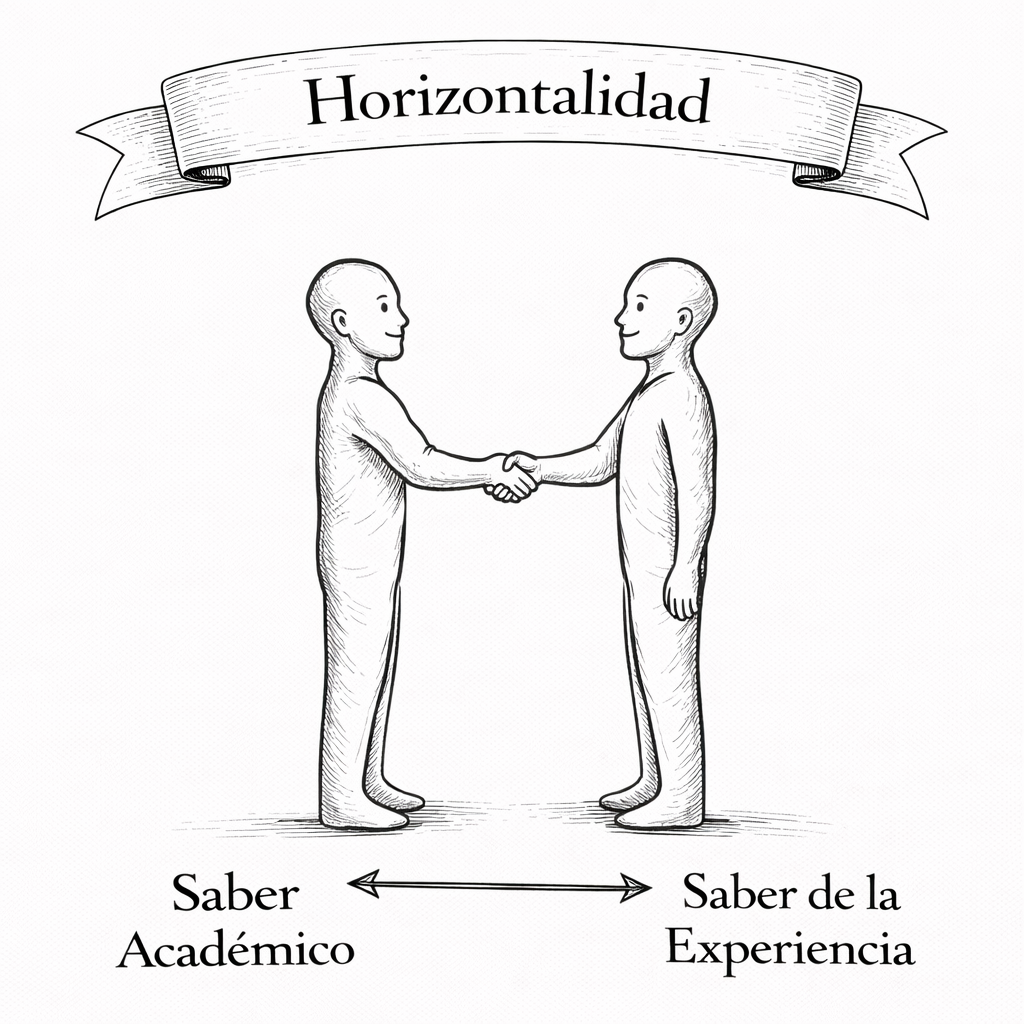
\includegraphics[scale=0.25]{343.png}
		\caption{La horizontalidad y complementariedad de los saberes}
	\end{figure}
	
	\momento{Fundamento o criterio de discernimiento} 
	La verdadera sanación ocurre cuando se establece un marco de cultura terapéutica basado en el vínculo comunitario\index{vínculo!comunitario|textbf}. La respuesta eclesial incorpora la especialización técnica como un elemento insustituible, pero la trasciende al integrarla en un modelo biopsicosocial-espiritual\index{modelo biopsicosocial-espiritual!y dignidad} donde el centro es la dignidad de la persona.
	
	La eficacia del acompañante par no se explica únicamente por su saber
	vivencial: radica también en que su sola presencia encarna lo que la
	psicología del \textit{recovery} denomina \textbf{identidad de recuperación}
	—la posibilidad concreta, visible y cercana, de ser otra cosa.
	
	\momento{Tesis y desarrollo argumental}\\ 
	La gestión de la tensión entre ambos saberes se resuelve mediante su integración armónica bajo los siguientes principios:
	
	\begin{enumerate}
		\item Reconocimiento de roles complementarios: El profesional aporta la técnica necesaria para abordar patologías duales o traumas complejos, mientras que el acompañante par aporta el arte del acompañamiento y la capacidad de llegar a la herida del otro desde un lugar de igualdad.
		\item Construcción horizontal de la red: El equipo debe funcionar como una familia, donde la mística del servicio rompe la jerarquía entre asistente y asistido, poniendo en valor el aporte específico de cada miembro.
		\item Diferenciación del acompañamiento: Se distingue entre un acompañamiento inespecífico (territorial), que es transversal y humaniza el recorrido, y un acompañamiento específico (profesional), que atiende aspectos clínicos, diagnósticos o legales puntuales.
		\item Formación compartida: Es fundamental que todo el equipo participe en procesos de capacitación mutua donde se valide tanto la ciencia como la sabiduría popular, permitiendo hablar un mismo idioma espiritual y técnico.
	\end{enumerate}
	
	\momento{Respuesta a las objeciones}
	\begin{itemize}
		\item \submomento{A la primera:} La técnica profesional corre el riesgo de ser ineficaz si se aplica de forma aislada. Solo cobra sentido cuando el paciente se siente en un ambiente de apego seguro que el saber territorial ayuda a construir y sostener.
		\item \submomento{A la segunda:} El saber territorial puede verse desbordado por situaciones de alta complejidad, como el riesgo suicida o descompensaciones psicóticas. La profesionalización dota de herramientas críticas al equipo y protege al cuidador del desgaste emocional y la fatiga por compasión. Se requiere, en definitiva, una misericordia estructurada que una la firmeza de la regla con la ternura del abrazo.
	\end{itemize}
	
	\newpage
	
	\section{Singularidad, diferencias sexuales y Nuevos Desafíos Digitales}
	
	Esta sección profundiza en la singularidad del sujeto, partiendo de la premisa de que el trastorno por uso de sustancias es un fenómeno que se agrega a la personalidad y no una estructura cerrada que define la identidad. Al reconocer que no existe un perfil único del consumidor, se propone un abordaje artesanal que considere las necesidades específicas de cada etapa del ciclo vital, desde la infancia hasta el consumo tardío en adultos mayores. Se analiza con rigor la vulnerabilidad de las mujeres, quienes enfrentan una doble condena social —por el consumo y por no cumplir roles tradicionales de cuidado—, además de verse mayormente afectadas por el trauma complejo y el abandono vincular. Asimismo, la mirada pastoral integra a la población travesti-trans, comprendiendo que en sus trayectorias la identidad, la exclusión y el consumo forman una misma trama de supervivencia ante la violencia sistémica. Finalmente, se aborda el impacto de las nuevas adicciones digitales, como las apuestas online, los videojuegos y la pornografía, reconociendo que estas conductas alteran los centros de placer cerebral mediante mecanismos de impulsividad y compulsividad análogos a los de las sustancias químicas.
	
	
	\subsection{Artículo 1: Sobre la vulnerabilidad y barreras de la mujer en el proceso de cambio}
	
	\momento{Planteo del tema} 
	La vulnerabilidad psicológica de la mujer en el ámbito de los consumos presenta una complejidad única que la distingue significativamente del varón. Esta diferencia no es solo biológica, sino que está profundamente marcada por el peso del trauma crónico, la sobrecarga de los roles de cuidado y una sanción social específica que castiga con mayor severidad a la mujer. Esta realidad dificulta tanto el acceso inicial a los dispositivos de salud como la permanencia en el proceso de recuperación.
	
	\momento{Pregunta central} 
	¿Se diferencia la vulnerabilidad psicológica de las mujeres de la de los hombres, y qué barreras específicas de acceso enfrentan en la recuperación?.
	
	\momento{Posturas u objeciones existentes}
	\begin{itemize}
		\item \submomento{Objeción 1:} Parece que el trastorno por uso de sustancias afecta por igual a hombres y mujeres, ya que la adicción es una enfermedad cerebral que no distingue sexo en sus mecanismos neurobiológicos de recompensa y dependencia.
		\item \submomento{Objeción 2:} Parece que las mujeres tienen mayores facilidades de acceso a tratamiento, dado que la sociedad tiende a ser más protectora con las madres y existen programas estatales específicos diseñados para la niñez y la familia.
	\end{itemize}
	
	\momento{Fundamento o criterio de discernimiento} 
	La mujer sufre una doble condena social: por el consumo en sí mismo y por no cumplir con el rol tradicional de madre o cuidadora. Esta realidad se traduce en una brecha de acceso crítica, donde las estadísticas indican que solo una de cada dieciocho mujeres con consumo problemático accede a tratamiento, en comparación con uno de cada siete hombres.
	
	\momento{Tesis y desarrollo argumental}\\ 
	Se debe decir que la vulnerabilidad de la mujer requiere un abordaje con perspectiva de género y sensibilidad al trauma, basándose en los siguientes pilares:
	
	\begin{enumerate}
		\item Efecto \marginnote{Cfr. art.~\ref{art:telescopio} (Juzgar, Las sustancias y el Organismo, Diferencias según..., La respuesta fisionógica...)}: Las mujeres suelen transitar de manera más acelerada que los hombres desde el primer uso hasta el desarrollo de un trastorno severo y sus consecuencias médicas. Esta progresión biopsicológica exige intervenciones tempranas y especializadas.
		\item El trauma complejo como precursor: La gran mayoría de las mujeres con adicciones han experimentado historias de trauma crónico, incluyendo violencia física, psicológica o abuso. El consumo funciona como un intento autoterapéutico de anestesiar dolores no resueltos y desregulaciones emocionales profundas.
		\item Sobrecarga de cuidados y estigma: La presión cultural por ser el sostén afectivo del hogar genera una internalización del rechazo social. El miedo a ser juzgadas como malas madres produce una culpa y vergüenza que paralizan la búsqueda de ayuda profesional.
		\item Abandono vincular y barreras estructurales: A diferencia de los varones, que suelen contar con el apoyo de sus parejas o madres, las mujeres son frecuentemente abandonadas por sus compañeros al iniciar un tratamiento. Además, existe una carencia de centros que permitan la internación con hijos, sumada a la amenaza de perder la custodia por parte del sistema judicial.
	\end{enumerate}
	
	\momento{Respuesta a las objeciones}
	\begin{itemize}
		\item \submomento{A la primera:} Aunque los mecanismos de recompensa cerebral sean análogos, los factores metabólicos y el contexto de violencia de género hacen que el impacto sea más devastador y rápido en la mujer. Ignorar la singularidad del género conduce a tratamientos ineficaces que no alojan la realidad subjetiva femenina.
		\item \submomento{A la segunda:} La supuesta protección institucional suele ser punitiva y burocrática en lugar de sanadora. La verdadera solución requiere programas receptivos al trauma y figuras de apego seguro que ofrezcan ternura en lugar de juicios morales, garantizando que el tratamiento no obligue a la mujer a elegir entre su recuperación y su maternidad.
	\end{itemize}
	
	
	\subsection{Artículo 2: Sobre la adaptación del abordaje según el ciclo vital}
	
	\momento{Planteo del tema} 
	La recuperación y la prevención no pueden ser procesos estandarizados que ignoren la biografía del sujeto. El desarrollo humano es un proceso dinámico donde las interacciones biológicas, psicológicas y ambientales cambian significativamente con el tiempo. Por ello, el acompañamiento debe ajustarse a la trayectoria vital de cada persona, reconociendo que la motivación, la percepción del riesgo y la vulnerabilidad neurológica varían drásticamente desde la niñez hasta la vejez.
	
	\momento{Pregunta central} 
	¿Debe el abordaje psicológico y pastoral adaptarse según la etapa del ciclo vital de la persona, o es suficiente un modelo estándar basado en la sustancia?.
	
	\momento{Posturas u objeciones existentes}
	\begin{itemize}
		\item \submomento{Objeción 1:} Parece que el abordaje debe centrarse primordialmente en la sustancia, ya que los efectos neuroquímicos de la droga y los criterios diagnósticos son similares independientemente de la edad del individuo.
		\item \submomento{Objeción 2:} Parece que los programas de prevención universal en las escuelas son suficientes para cubrir todas las etapas tempranas, minimizando la necesidad de intervenciones específicas para niños o adolescentes.
		\item \submomento{Objeción 3:} Parece que el consumo en adultos mayores es una problemática menor o inexistente, por lo que no se considera necesario desarrollar estrategias específicas para quienes han superado la edad laboral.
	\end{itemize}
	
	\momento{Fundamento o criterio de discernimiento} 
	No existe un perfil único del consumidor. El abordaje integral exige programas apropiados para la edad y la dosificación del riesgo, entendiendo que cada etapa evolutiva presenta desafíos y potencialidades únicas para la sanación.
	
	\momento{Tesis y desarrollo argumental}\\ 
	El abordaje debe organizarse de forma artesanal según las necesidades específicas de cada etapa del ciclo vital:
	
	\begin{enumerate}
		\item Infancia (6 a 11 años): El foco se sitúa en la socialización y el desarrollo de habilidades básicas como la regulación de impulsos y la atención. Las intervenciones deben fortalecer el apego seguro y la autoestima, reconociendo que un inicio temprano (8 o 9 años) impide la formación sana de las redes neuronales.
		\item Adolescencia (12 a 17 años): Es la etapa de mayor riesgo biológico porque la corteza prefrontal\marginnote{Cfr. art.~\ref{art:cortex} (Juzgar, Las sustancias y el organismo, Definición..., Riesgos...)} —el freno del cerebro— aún no ha madurado, mientras que el sistema de recompensa es altamente sensible. El trabajo debe centrarse en la resistencia a la presión de grupo, la autoeficacia y la construcción de una identidad independiente de la sustancia.
		\item Vida Adulta: El tratamiento se orienta hacia la recuperación de roles sociales, la inclusión laboral, la reeducación financiera y la reconstrucción de vínculos familiares dañados por años de consumo, buscando una autonomía progresiva.
		\item Adultos Mayores: Es fundamental abordar el consumo tardío, frecuentemente ligado a la jubilación, la soledad o el duelo. La motivación para el cambio en esta etapa se vincula a la búsqueda de sentido frente al final de la vida y al manejo de una metabolización más lenta de las sustancias.
	\end{enumerate}
	
	\momento{Respuesta a las objeciones}
	\begin{itemize}
		\item \submomento{A la primera:} Aunque la molécula sea la misma, el impacto en un cerebro en desarrollo causa deficiencias cognitivas permanentes que no ocurren igual en un adulto, lo que exige estrategias pedagógicas y clínicas diferenciadas.
		\item \submomento{A la segunda:} La prevención universal es necesaria pero insuficiente para grupos de alta vulnerabilidad, como hijos de personas con trastornos por uso de sustancias, quienes requieren intervenciones que aborden directamente el trauma y las carencias emocionales.
		\item \submomento{A la tercera:} El consumo en la tercera edad es una realidad invisibilizada por el estigma. El acompañamiento debe devolver la dignidad existencial a los adultos mayores, integrándolos en la comunidad para que no enfrenten su dependencia en la soledad del aislamiento social.
	\end{itemize}
	
	\subsection{Artículo 3: Sobre el abordaje de las adicciones digitales}
	
	\momento{Planteo del tema} 
	
	El abordaje de las denominadas adicciones digitales —que incluyen 
	los videojuegos, las apuestas online y la pornografía— exige 
	comprender la transición de los trastornos del impulso hacia las 
	adicciones conductuales. En estos cuadros, se produce una disfunción 
	en el sistema de recompensa cerebral donde la liberación de dopamina\marginnote{Cfr. art.~\ref{art:dopamina} (Juzgar, Las sustancias y el organismo, La farmacodinámica..., Art. 1...)} 
	refuerza hábitos compulsivos de manera análoga a lo que ocurre con 
	las sustancias químicas. No se trata simplemente de un uso excesivo 
	de la tecnología, sino de una alteración en la capacidad de regulación 
	que compromete la libertad del sujeto frente al dispositivo.
	
	\momento{Pregunta central} 
	¿Deben las adicciones digitales abordarse bajo los mismos criterios psicológicos que las adicciones a sustancias, considerando que activan circuitos cerebrales similares?.
	
	\momento{Posturas u objeciones existentes}
	\begin{itemize}
		\item \submomento{Objeción 1:} Parece que las conductas digitales no pueden considerarse adicciones reales, pues en ellas no existe el ingreso de una molécula externa al organismo que produzca un impacto neurobiológico verificable.
		\item \submomento{Objeción 2:} Parece que estas conductas son simples problemas de falta de disciplina o impulsividad, especialmente en jóvenes, y que no presentan un síndrome de abstinencia biológico como el de las drogas.
		\item \submomento{Objeción 3:} Se afirma que la única solución efectiva ante el riesgo del ambiente digital es la prohibición total de la tecnología para evitar el aislamiento y la manipulación que este entorno propicia.
	\end{itemize}
	
	\momento{Fundamento o criterio de discernimiento} 
	Aunque no medie una sustancia química ingerida, estas conductas alteran los centros de placer y recompensa del cerebro de forma similar a las drogas. El abordaje debe reconocer que el ambiente digital puede exponer a la persona a la dependencia y a la pérdida de contacto con la realidad concreta, requiriendo una reeducación de la voluntad.
	
	\momento{Tesis y desarrollo argumental}\\ 
	Se debe decir que el tratamiento de las adicciones digitales requiere un enfoque integral que considere la dinámica de la compulsión y el malestar subyacente, basándose en los siguientes pilares:
	
	\begin{enumerate}
		\item Diferenciación entre impulsividad y compulsividad: La impulsividad está motivada por la búsqueda de placer inmediato, mientras que la compulsividad busca evitar o reducir emociones negativas. El tratamiento debe identificar en qué punto el placer se transforma en una necesidad de evasión.
		\item Identificación del dolor primario: El enfoque psicológico no debe quedarse en la conducta externa, sino indagar en el malestar emocional, el fracaso o la incertidumbre que el individuo intenta anestesiar a través del dispositivo.
		\item Manejo del dolor secundario: La evasión digital genera un nuevo nivel de sufrimiento marcado por la culpa, la vergüenza y la ansiedad social. Trabajar estos sentimientos es esencial para romper el ciclo de consumo digital.
		\item Terapia de Aceptación y Compromiso (ACT): Se utiliza para ayudar al sujeto a afrontar sus realidades internas y tolerar el malestar sin buscar el refugio inmediato de la pantalla, fortaleciendo su compromiso con valores de vida reales.
		\item Atención al estrés digital y FOMO: El abordaje debe tratar la alerta constante y el miedo a quedar fuera de la conexión (Fear of Missing Out), que generan sobrecarga de información y una ansiedad persistente por la aprobación externa.
	\end{enumerate}
	
	\momento{Respuesta a las objeciones}
	\begin{itemize}
		\item \submomento{A la primera:} Aunque no hay químicos externos, el cerebro procesa estas experiencias mediante procesos neuroplásticos. La exposición constante a estímulos digitales cambia físicamente los circuitos cerebrales de manera similar al aprendizaje de cualquier hábito adictivo.
		\item \submomento{A la segunda:} La experiencia clínica demuestra que los usuarios presentan obsesión mental y síntomas físicos de abstinencia, como irritabilidad o malestar, cuando no acceden a la red. El diseño de estas plataformas busca precisamente vencer el autocontrol, especialmente en adolescentes con una corteza prefrontal\marginnote{Cfr. art.~\ref{art:cortex} (Juzgar, Las sustancias y el organismo, Definición..., Riesgos...)} aún inmadura.
		\item \submomento{A la tercera:} El objetivo no es la supresión de la tecnología, sino el desarrollo de una ciudadanía digital responsable. Se busca que la parte racional del cerebro recupere el mando sobre los impulsos emocionales, transformando la tecnología en una herramienta para el estudio y el encuentro humano.
	\end{itemize}
	
	\newpage
	
	\section{Habilidades de Acompañamiento y Autocuidado}
	
	Esta sección profundiza en el arte del acompañamiento, donde se propone la escucha activa\index{escucha} y empática no solo como una técnica, sino como el primer medicamento capaz de humanizar el recorrido de quien sufre y reconocer su dignidad como tierra sagrada. Se detallan habilidades fundamentales como el parafraseo, el resumen y la afirmación, orientadas a despertar la autoeficacia y el protagonismo de la persona en su propio proceso de transformación. De manera complementaria y vital, la sección aborda la urgencia de cuidar a los que cuidan, reconociendo la vulnerabilidad del sanador herido y la necesidad imperante de prevenir el agotamiento profesional o la fatiga por compasión en contextos de alta complejidad. Finalmente, se reivindica el descanso y el establecimiento de límites sanos\index{límite sano} como dimensiones esenciales de la misión, instando a los agentes pastorales a dejarse sostener por la comunidad para que el servicio sea sostenible y refleje siempre la ternura del encuentro humano.
	
	\begin{figure}[h!]
		\centering
		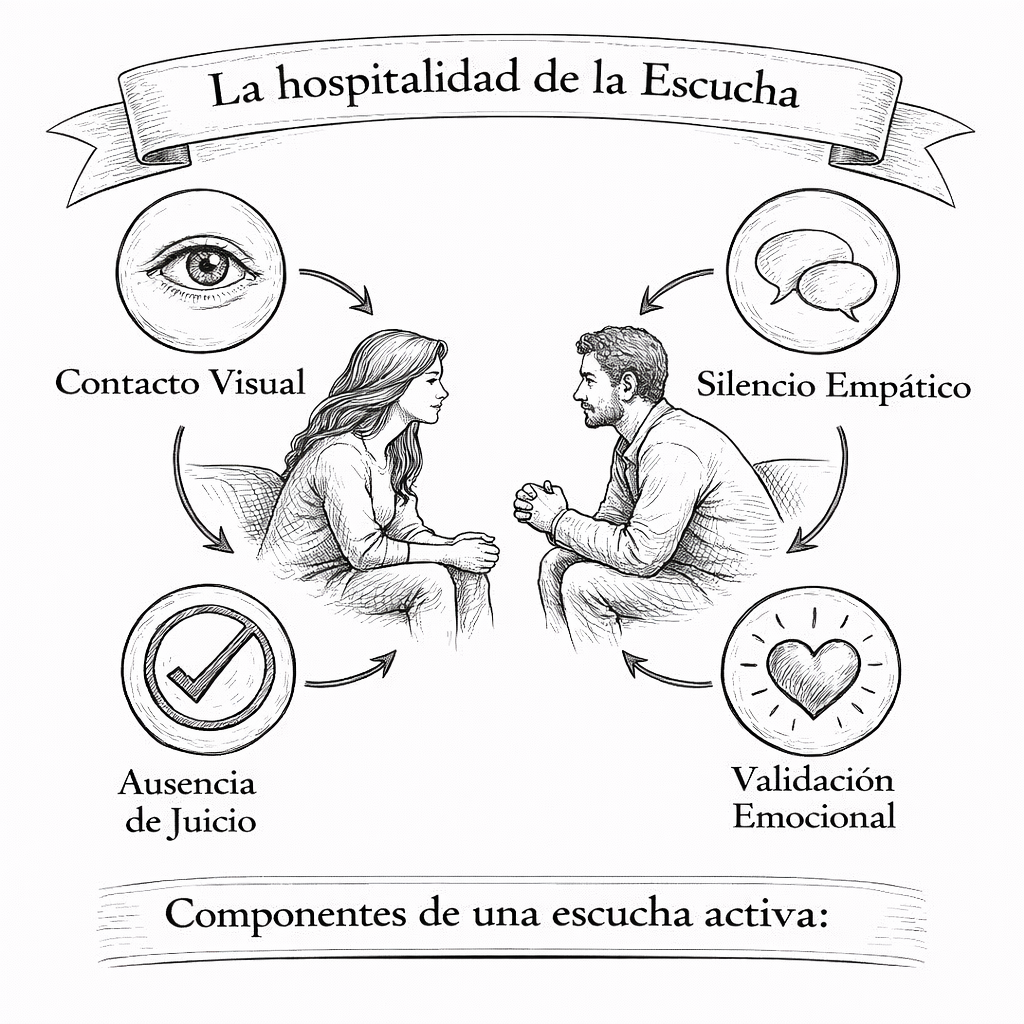
\includegraphics[scale=0.25]{341.png}
		\caption{La escucha activa}
	\end{figure}
	
	\subsection{Artículo 1: Sobre la naturaleza de la escucha activa y el trabajo interior del acompañante}
	
	\marginnote{Sant 1, 19\label{sant1.19} — \textit{Sepan, hermanos míos queridos, que cada uno debe estar dispuesto a escuchar, y ser lento para hablar y para encolerizarse}}
	
	\momento{Planteo del tema} 
	La escucha activa\index{escucha|textbf} se propone como el primer medicamento en el proceso de recuperación, siendo una habilidad compleja que trasciende el simple silencio. Requiere una receptividad intensa, concentración y paciencia para constituirse como un acto de hospitalidad\index{hospitalidad} hacia el corazón del otro. No se trata de una técnica mecánica, sino de una disposición espiritual y psicológica que busca humanizar el recorrido de quien sufre, reconociendo su historia como una tierra sagrada que debe ser tratada con máximo respeto.
	
	\momento{Pregunta central} 
	¿Cuáles son los componentes esenciales de la escucha activa y qué obstáculos internos debe trabajar el acompañante para lograr un vínculo sanador?.
	
	\momento{Posturas u objeciones existentes}
	\begin{itemize}
		\item \submomento{Objeción 1:} Parece que escuchar es un proceso meramente pasivo que consiste en guardar silencio mientras el otro habla, por lo que no se requeriría una formación específica ni una actitud deliberada.
		\item \submomento{Objeción 2:} Parece que la función principal del acompañante es ser un consejero que debe tener respuestas preparadas; centrarse solo en escuchar podría retrasar la intervención correctiva necesaria.
		\item \submomento{Objeción 3:} Se asume que el contenido de la comunicación es únicamente verbal, por lo que prestar atención a las señales físicas o al lenguaje corporal sería secundario frente a la literalidad de las palabras.
	\end{itemize}
	
	\momento{Fundamento o criterio de discernimiento} 
	La escucha activa es una herramienta fundamental diseñada para que la persona se sienta atendida y considerada. No busca imponer una verdad externa, sino permitir que aparezca la historia de vida del sujeto\index{escucha!componentes esenciales}, validando su palabra como el eje de su propia transformación.
	
	\momento{Tesis y desarrollo argumental}\\ 
	La escucha activa se fundamenta en componentes técnicos precisos y en un trabajo profundo sobre la interioridad del acompañante:
	
	\begin{enumerate}
		\item Componentes técnicos:
		\begin{itemize}
			\item Atención activa: Implica preocuparse por todos los niveles de comunicación (verbal y no verbal), comunicando presencia mediante el contacto visual y gestos de aliento.
			\item Parafraseo: Consiste en repetir el contenido expresado utilizando las propias palabras para verificar la comprensión y demostrar que el mensaje ha sido captado.
			\item Reflejo de sentimientos: El acompañante intenta percibir y expresar el estado emocional del otro, demostrando empatía al compartir la comprensión de su punto de vista sin juzgarlo.
			\item Resumen: Reúne los puntos principales de la conversación para evitar malentendidos y preparar al sujeto para el siguiente paso en su proceso.
		\end{itemize}
		\item Obstáculos internos del acompañante: El vínculo sanador exige remover barreras como la reactividad emocional, la autorreferencialidad (pensar en la propia respuesta mientras el otro habla) y los prejuicios que llevan a calificar las acciones ajenas como viciosas.
	\end{enumerate}
	
	\momento{Respuesta a las objeciones}
	\begin{itemize}
		\item \submomento{A la primera:} La escucha es activa\index{escucha!por qué activa} porque requiere una participación dinámica del sistema nervioso y la voluntad de sintonizar con el mundo interior ajeno. No es ausencia de acción, sino una presencia plena y consciente.
		\item \submomento{A la segunda:} El objetivo no es ser un sabio que imparte lecciones, sino un guía al costado. La persona sana cuando puede simbolizar su propio dolor a través de la palabra, recuperando su autonomía en lugar de recibir órdenes.
		\item \submomento{A la tercera:} La comunicación es integral. Las señales no verbales a menudo revelan más sobre el sufrimiento que el discurso racionalizado; por ello, la atención a lo corporal es indispensable para captar la totalidad del mensaje.
	\end{itemize}
	
	\subsection{Artículo 2: Sobre la autoeficacia, la afirmación y la persuasión social}
	
	\momento{Planteo del tema} 
	La recuperación de las adicciones requiere que el sujeto recupere la confianza en su propia capacidad para generar cambios. El desarrollo de la autoeficacia no es un proceso que ocurra en el aislamiento, sino que se nutre constantemente de la interacción con el entorno y el acompañamiento. A través de la afirmación y la persuasión social, el acompañante actúa como un espejo que devuelve al individuo una imagen de sus propias fortalezas, permitiéndole transitar desde la parálisis de la duda hacia una actitud de protagonismo en su proyecto de vida.
	
	\momento{Pregunta central} 
	¿Influye el desarrollo de la autoeficacia, mediado por la afirmación y la persuasión social, de manera determinante en el fortalecimiento del proceso terapéutico?.
	
	\momento{Posturas u objeciones existentes}
	\begin{itemize}
		\item \submomento{Objeción 1:} Parece que la autoeficacia es un rasgo innato de la personalidad o una fuerza de voluntad interna que el sujeto posee o no posee, por lo que los estímulos externos o las palabras del acompañante no tendrían un impacto real en la conducta.
		\item \submomento{Objeción 2:} Parece que la afirmación constante podría ser contraproducente, ya que al resaltar aspectos positivos en alguien que ha cometido errores graves se corre el riesgo de minimizar la enfermedad o fomentar una falsa confianza que ignore los riesgos de recaída.
		\item \submomento{Objeción 3:} Parece que la persuasión social es un recurso superficial que no aborda las modificaciones estructurales en el cerebro causadas por el consumo; sin una reparación biológica previa, ninguna palabra de aliento podrá restaurar la capacidad de decidir.
	\end{itemize}
	
	\momento{Fundamento o criterio de discernimiento} 
	La autoeficacia\index{autoeficacia|textbf} es la creencia de una persona en su habilidad para tener éxito en una situación particular. Recibir estímulo verbal y afirmación de otros ayuda a superar las dudas e incrementa la capacidad de tomar acción, transformando la motivación de un estado fluctuante a un compromiso firme con el cambio.
	
	\momento{Tesis y desarrollo argumental}\\ 
	Se debe decir que el desarrollo de la autoeficacia\index{autoeficacia!como motor del cambio} es el motor del cambio en el proceso terapéutico, manifestándose a través de los siguientes ejes:
	
	\begin{enumerate}
		\item La afirmación como validación del ser: Afirmar implica realizar declaraciones sinceras y positivas que validan a la persona más allá de sus actos. Esta práctica refuerza los éxitos pequeños, fortalece la alianza terapéutica y demuestra que el acompañante reconoce el esfuerzo y el valor intrínseco del sujeto.
		\item La persuasión social como antídoto a la duda: En contextos de exclusión, el usuario suele internalizar mensajes de fracaso. La palabra del acompañante actúa como una fuerza externa que permite al individuo reconsiderar su potencial, creyendo en sus habilidades para triunfar antes incluso de que él mismo pueda percibirlas.
		\item Prevención del desaliento: Al enfatizar las experiencias que demuestran fortaleza, la afirmación ayuda a la persona a transitar del sentimiento de  no me lo merezco  hacia una convicción de  puedo hacerlo , lo cual es vital para sostener el esfuerzo en las etapas iniciales de la recuperación.
		\item Sostenibilidad en etapas críticas: Tanto en la fase de acción como en la de mantenimiento, la afirmación constante ayuda a normalizar la ambivalencia y fortalece la capacidad de gestionar nuevas estrategias de afrontamiento sin recurrir a la sustancia.
	\end{enumerate}
	
	\momento{Respuesta a las objeciones}
	\begin{itemize}
		\item \submomento{A la primera:} Aunque la autoeficacia\index{autoeficacia!y persuasión social} es una creencia interna, se nutre de modelos y mentores. La motivación interna a menudo se despierta a través de la persuasión social de alguien que confía en el usuario, proporcionando el impulso necesario para que el sujeto comience a confiar en sí mismo.
		\item \submomento{A la segunda:} La afirmación no ignora la realidad de la enfermedad, sino que separa la conducta de la identidad. Transformar pensamientos irracionales de culpa en afirmaciones basadas en fortalezas es un requisito indispensable para que la persona asuma la responsabilidad de su propio proceso.
		\item \submomento{A la tercera:} Si bien el cerebro está afectado, el estímulo verbal y la confianza comunitaria actúan como reforzadores que facilitan el aprendizaje de nuevos hábitos. Se aprovecha la neuroplasticidad\marginnote{Cfr. art.~\ref{art:neuroplasticidad} (Juzgar, Brevísimo Glosario)} para que la parte racional del cerebro retome el mando sobre los impulsos emocionales, estabilizando así la conducta saludable.
	\end{itemize}
	
	\subsection{Artículo 3: Sobre la introspección y el diario de emociones}
	
	\momento{Planteo del tema} 
	La introspección y el uso de herramientas como el diario de emociones se proponen como instrumentos de humanización del recorrido. No son meros ejercicios intelectuales, sino actos de mirar hacia adentro para realizar una reflexión profunda sobre los sentimientos y el comportamiento. Esta práctica es un punto esencial para el crecimiento personal, permitiendo que el individuo encuentre paz y plenitud al profundizar en su propio ser y en la verdad de su historia.
	
	\momento{Pregunta central} 
	¿Tienen la introspección y el uso de herramientas como el diario de emociones una importancia fundamental para el autoconocimiento y la recuperación del paciente?.
	
	\momento{Posturas u objeciones existentes}
	\begin{itemize}
		\item \submomento{Objeción 1:} Parece que la introspección no es conveniente para personas con trastornos por uso de sustancias, pues al poseer redes de memoria cargadas de trauma, mirar hacia adentro solo aumentaría su angustia y desesperación.
		\item \submomento{Objeción 2:} Parece que el uso de herramientas escritas es ineficaz o excluyente, dado que muchos pacientes en situación de vulnerabilidad extrema presentan un bajo nivel de escolaridad o deterioro cognitivo que les impide realizar reflexiones escritas.
		\item \submomento{Objeción 3:} Se afirma que lo más importante es el servicio y la acción comunitaria bajo la premisa de que el trabajo sana, por lo que la reflexión interna sería un ejercicio secundario frente a la urgencia de la reintegración social.
	\end{itemize}
	
	\momento{Fundamento o criterio de discernimiento} 
	La introspección es el acto de reflexión interna necesario para el crecimiento personal. El autoconocimiento ayuda a profundizar en el propio ser para encontrar un sentido de vida trascendente, transformando al individuo de un objeto de asistencia en un sujeto consciente de su dignidad.
	
	\momento{Tesis y desarrollo argumental}\\ 
	La introspección y el registro emocional son fundamentales para la recuperación porque permiten abordar la raíz del sufrimiento bajo los siguientes pilares:
	
	\begin{enumerate}
		\item Identificación de la fractura interna: Permite que el paciente deje de ver la droga como el problema central y comience a entenderla como un síntoma de un dolor profundo o abandono previo. Sin este ejercicio, el tratamiento solo toca la superficie sin sanar la causa.
		\item Facilitación del darse cuenta: El registro de emociones ayuda a identificar conductas negativas y pensamientos rígidos. Este proceso convierte al sujeto en un protagonista que asume la responsabilidad de su propia historia.
		\item Ordenamiento del mundo interno: El diario funciona como un ancla frente al caos de la vida de calle. Al nombrar lo que siente, el paciente permite que la parte racional del cerebro recupere el control sobre los impulsos emocionales.
		\item Vinculación con la trascendencia: Desde la perspectiva pastoral, la introspección se eleva al examen de conciencia, donde la persona reconoce la presencia de Dios en su jornada y fortalece su voluntad para el cambio.
	\end{enumerate}
	
	\momento{Respuesta a las objeciones}
	\begin{itemize}
		\item \submomento{A la primera:} Aunque mirar el trauma es doloroso, la sanación integral solo es posible mediante la resignificación de esos eventos. La comunidad debe proporcionar el lugar seguro para que esta introspección no sea un acto solitario, sino un proceso acompañado y contenido.
		\item \submomento{A la segunda:} La herramienta debe ser artesanal y flexible. En casos de baja escolaridad, la introspección puede facilitarse mediante el diálogo empático, el arte o el acompañamiento de pares que ayuden al sujeto a poner en palabras lo que siente.
		\item \submomento{A la tercera:} No hay oposición entre acción e introspección, pues el ser humano es una unidad de cuerpo y alma. El servicio comunitario cobra su verdadero sentido cuando nace de un corazón que se conoce a sí mismo y ha descubierto su dignidad ante Dios.
	\end{itemize}
	
	\subsection{Artículo 4: Sobre la necesidad vital del autocuidado para los agentes pastorales}
	
	\momento{Planteo del tema} 
	El acompañamiento a personas en situaciones de vulnerabilidad extrema y consumo problemático implica un elevado costo emocional que, de no gestionarse adecuadamente, deriva en agotamiento profesional\index{burnout}, fatiga por compasión o vacío existencial. Quienes realizan esta labor se encuentran en un escenario de alta complejidad donde la frustración puede ser frecuente. Por ello, el autocuidado\index{autocuidado} no debe considerarse un complemento opcional, sino una dimensión intrínseca y vital de la misión que garantiza que el servicio sea humanizante y sostenible en el tiempo.
	
	\momento{Pregunta central} 
	¿Es vital integrar un módulo de autocuidado para los agentes pastorales con el fin de prevenir el desgaste por empatía, el burnout y la fatiga por compasión?.
	
	\momento{Posturas u objeciones existentes}
	\begin{itemize}
		\item \submomento{Objeción 1:} Parece que el acompañamiento es un sacrificio total que debe asumirse como una participación en la cruz de Cristo, por lo que el cansancio del agente sería una entrega necesaria que no requeriría un módulo de autocuidado.
		\item \submomento{Objeción 2:} Parece que los recursos y el tiempo deben centrarse exclusivamente en el usuario, considerando que el bienestar de los agentes pastorales es un lujo o una distracción de la urgencia de salvar vidas.
		\item \submomento{Objeción 3:} Se afirma que la fe y la oración son suficientes para sostener al cuidador, sugiriendo que el agotamiento se debe únicamente a una falta de vida espiritual y no a una necesidad de estrategias psicológicas de cuidado.
	\end{itemize}
	
	\begin{figure}[h!]
		\centering
		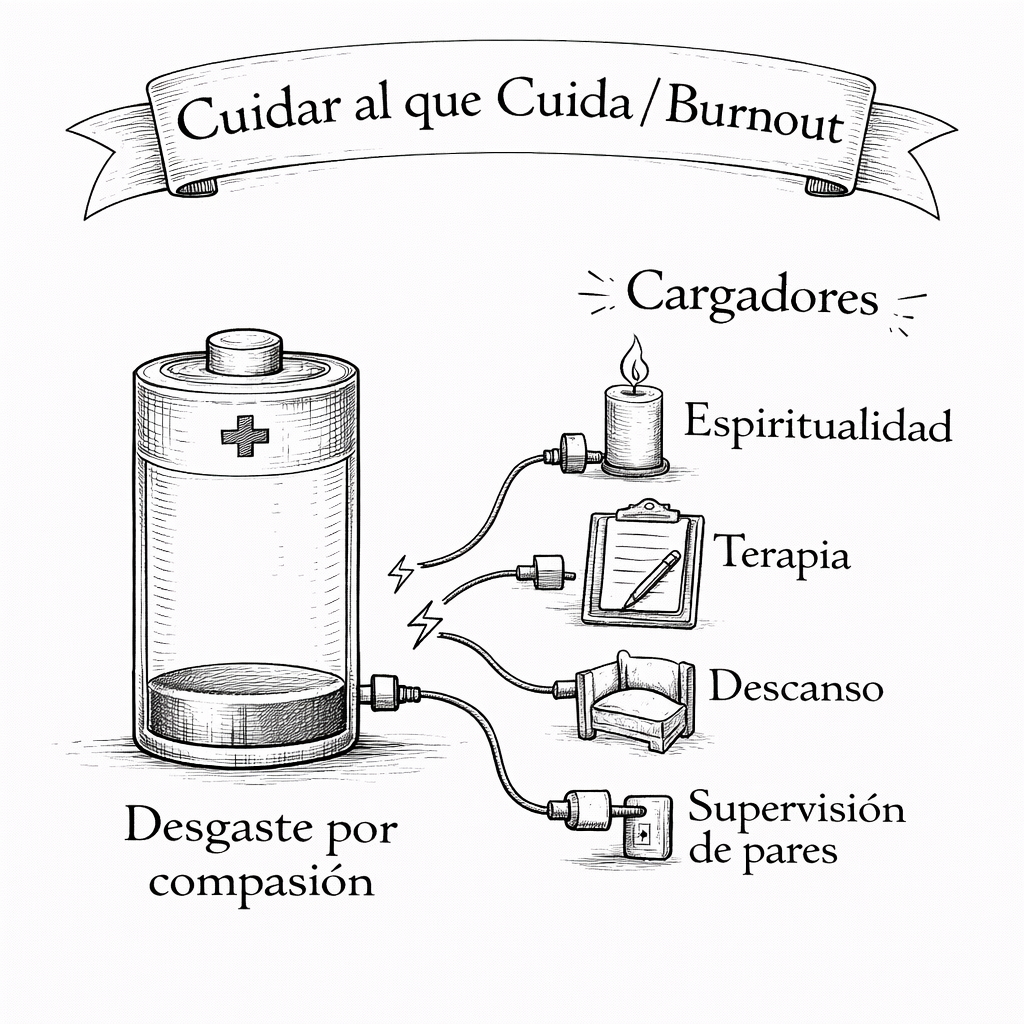
\includegraphics[scale=0.25]{361.png}
		\caption{Cuidar al que cuida}
	\end{figure}
	
	\momento{Fundamento o criterio de discernimiento} 
	El descanso es una necesidad humana y espiritual ordenada por el propio Cristo para quienes están en el centro del servicio. El acompañamiento integral exige que el agente gestione su propia vida y reconozca sus límites para evitar que la antorcha de la esperanza se apague, entendiendo que el derecho al ocio es una dimensión esencial de la misión.
	
	\momento{Tesis y desarrollo argumental}\\ 
	La integración de un módulo de autocuidado es un acto de justicia y responsabilidad misionera que se fundamenta en los siguientes pilares:
	
	\begin{enumerate}
		\item Sostenibilidad de la misión: Para cuidar bien es imperativo que el agente preserve su propia salud. El agotamiento extremo impide la continuidad de la tarea y hace que el servicio se vuelva insostenible, afectando la calidad del acompañamiento a largo plazo.
		\item Prevención del trauma secundario: Los cuidadores están expuestos a un estrés postraumático derivado de cargar con el dolor y las heridas de los usuarios. Contar con protocolos de detección de burnout\index{burnout!protocolos de detección} y fatiga por compasión permite procesar este impacto y evita que los agentes pastorales somaticen el sufrimiento ajeno.
		\item Identidad del sanador herido: El\index{autocuidado!sanador herido|textbf} acompañante debe reconocer su propia vulnerabilidad y necesidad de ternura. Aceptar las propias llagas permite que el pastor se deje cuidar por la comunidad, evitando situarse en una posición de superioridad que bloquee el vínculo real.
		\item Calidad del cuidado: Un agente pastoral desgastado pierde la capacidad de escucha activa y de empatía. El autocuidado permite realizar las pausas necesarias para asegurar que el encuentro con el otro sea siempre un gesto de amor y no una carga mecánica o burocrática.
		\item Establecimiento de límites sanos\index{límite sano!para el agente pastoral}: El cuidado implica aprender a decir no y a retirarse al  banco de suplentes  cuando las fuerzas flaquean, reconociendo que nadie puede solo y que la comunidad es el soporte último de la tarea.
	\end{enumerate}
	
	\momento{Respuesta a las objeciones}
	\begin{itemize}
		\item \submomento{A la primera:} Aunque la entrega generosa es valiosa, Dios no pide sacrificios que destruyan la propia vida. Cuidar de uno mismo es una forma de honrar el don de la vida y garantizar que el servicio pueda continuar sin que el cuidador se quiebre.
		\item \submomento{A la segunda:} El autocuidado es una estrategia de salud mental indispensable, no un lujo. Invertir en el bienestar del equipo garantiza que siempre haya manos disponibles y mentes claras para atender la emergencia social de forma eficaz.
		\item \submomento{A la tercera:} La fe no anula la biología ni las leyes de la psiquis. Es necesario integrar la vida espiritual con hábitos saludables, ejercicio y apoyo entre pares para que la salud integral del agente esté en óptimas condiciones para la misión.
	\end{itemize}
	
	\chapter{Las sustancias y el organismo}
	
	\momento{Planteo del tema: Las sustancias y el organismo.} El estudio de la relación entre el ser humano y las sustancias químicas implica comprender cómo ciertos componentes externos interactúan con la estructura biológica más compleja del hombre: su sistema nervioso. Esta interacción no es un evento aislado, sino un proceso farmacológico y metabólico que altera la percepción y el comportamiento del individuo.
	
	\newpage
	
	\section{Definición y Clasificación de las Sustancias}
	
	Una \textbf{sustancia psicoactiva (SPA)} es cualquier compuesto químico que, al introducirse en el organismo, \textbf{afecta el funcionamiento del sistema nervioso central (SNC)}, modificando el comportamiento, la percepción o el estado de ánimo. Para actuar directamente sobre las neuronas, estas sustancias deben ser capaces de \textbf{atravesar la barrera hematoencefálica (BHE)}\index{barrera hematoencefálica|textbf}, una frontera biológica que protege al cerebro y que resulta impermeable para la mayoría de los compuestos químicos.
	
	Según el efecto específico que provocan al interactuar con el cerebro, se clasifican actualmente en seis grupos fundamentales: \textbf{estimulantes, depresores, opioides, alucinógenos, disociativos y cannabinoides}.
	
	Es fundamental reconocer que sustancias legales como el \textbf{alcohol, la nicotina y la cafeína} son sustancias psicoactivas, ya que cumplen estrictamente con el criterio biológico de alterar el SNC, independientemente de su aceptación social. En la actualidad, el riesgo sanitario se ha agravado con la aparición de \textbf{nuevas sustancias psicoactivas (NSP)} y \textbf{opioides sintéticos como el fentanilo}, cuya potencia es \textbf{hasta cien veces superior} a la de drogas tradicionales, elevando el peligro de muerte por sobredosis debido a su dosificación impredecible y su uso frecuente como adulterante oculto.
	
	
	\subsection{Artículo 1: Definición de las sustancias psicoactivas (SPA)}
	
	\momento{Planteo del tema: La interacción química con el sistema nervioso}\\
	El estudio de la relación entre el ser humano y las sustancias implica comprender cómo ciertos componentes externos logran interactuar con la estructura biológica más compleja del hombre: su sistema nervioso. Esta interacción no es un evento aleatorio, sino un proceso farmacológico definido por la capacidad de una molécula para alterar la percepción, el humor y el comportamiento del individuo.
	
	\momento{Pregunta central}\\
	¿Qué define a una sustancia como <<psicoactiva>> y qué diferencia su paso por el organismo del de un medicamento común?
	
	\momento{Posturas u objeciones existentes}
	
	\begin{enumerate}
		\def\labelenumi{\arabic{enumi}.}
		
		\item
		\textbf{Parece que el término se refiere únicamente a las drogas ilícitas}, asociando la psicoactividad solo con sustancias prohibidas.
		
		\item
		\textbf{Parece que estas sustancias solo afectan la <<mente>>}, sin tener una repercusión real en el resto del organismo físico.
		\item
		\textbf{Parece que no hay diferencia entre una SPA y cualquier medicamento común} (como un antibiótico), ya que ambos se ingieren para producir un efecto en la salud.
		\item
		\textbf{Parece que las adicciones conductuales son equivalentes}, pues alteran el placer sin necesidad de un químico externo.
	\end{enumerate}
	
	\momento{Fundamento o criterio de discernimiento} Contra esto, el criterio científico establece que una SPA es un componente que afecta al sistema nervioso central (SNC) mediante una capacidad farmacológica específica: la de cruzar defensas biológicas que otros componentes no pueden atravesar.
	
	\momento{Tesis y desarrollo argumental}\\ Respondemos que las sustancias psicoactivas son componentes químicos de \textbf{estructura molecular pequeña y liposolubles} (solubles en grasas). Estas dos características son las que les otorgan la \textit{llave} técnica para cruzar la \textbf{barrera hematoencefálica (BHE)}\index{barrera hematoencefálica!mecanismo de cruce}, una membrana protectora compuesta por células unidas de forma muy ajustada que restringe el flujo de químicos hacia el cerebro. 
	
	Aunque la liposolubilidad y el tamaño molecular pequeño constituyen la vía de acceso predominante de las SPA al tejido cerebral, la farmacología reconoce también otros mecanismos de paso a través de la BHE, como el transporte activo y el transporte facilitado, mediante los cuales ciertas moléculas son trasladadas por proteínas transportadoras especializadas. Asimismo, la BHE no es uniformemente impermeable en todas las regiones del cerebro: determinadas zonas denominadas órganos circunventriculares presentan una barrera más permeable, lo que permite el intercambio de señales químicas entre la sangre y el sistema nervioso central. Estas precisiones no alteran el criterio general aquí expuesto, pero completan el panorama para el lector que desee profundizar en la materia.
	
	Hecha esta precisión, conviene señalar que la mayoría de los medicamentos comunes son hidrosolubles (se disuelven en agua) y poseen moléculas grandes que la BHE bloquea efectivamente. Las SPA, en cambio, aprovechan su afinidad con las membranas grasas de la barrera para acceder directamente al tejido cerebral. Una vez dentro, actúan de las siguientes formas:
	
	\begin{figure}[h]
		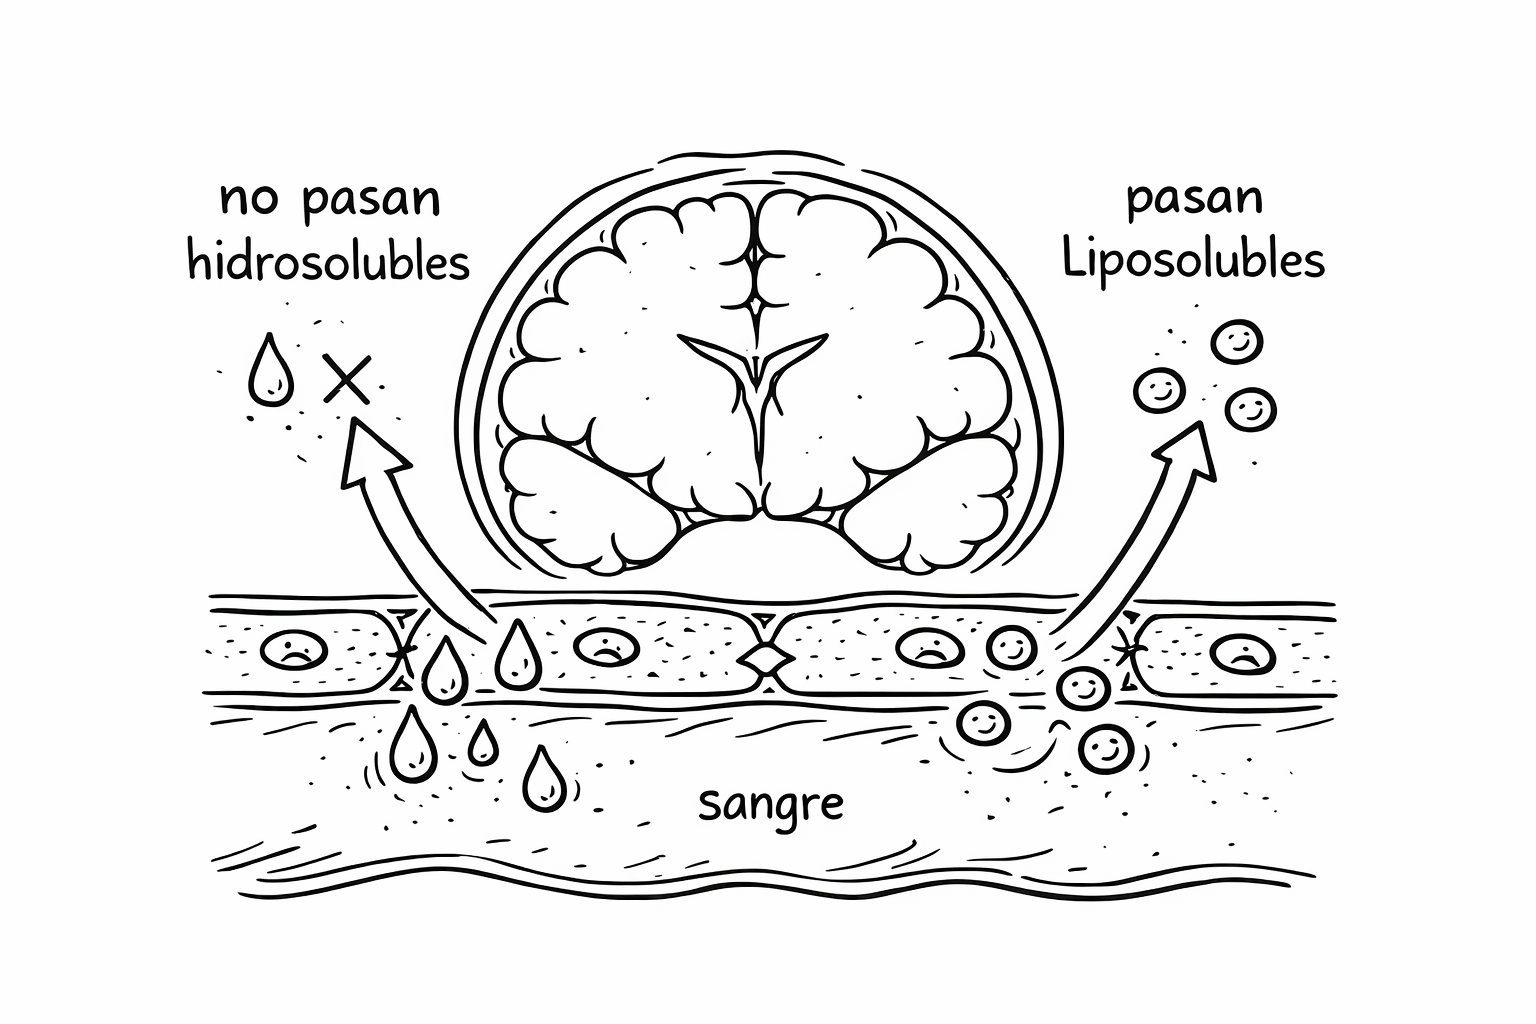
\includegraphics[scale=0.275]{barrera hematoencefalica.png}
		\caption{Barrera Hematoencefalica}
	\end{figure}
	
	Una vez que atraviesan esta barrera, las sustancias psicoactivas actúan de las siguientes formas:
	
	\begin{itemize}
		
		\item
		\textbf{Interferencia en la comunicación:} Alteran la manera en que las neuronas envían, reciben y procesan las señales de los neurotransmisores en el espacio intersináptico.
		\item
		\textbf{Clasificación funcional:} Según su efecto, se dividen en \textbf{estimulantes, depresores, opioides, alucinógenos, disociativos y cannabinoides}.
		\item
		\textbf{Proceso metabólico:} El cuerpo busca neutralizarlas a través del hígado y los riñones. El impacto de una sustancia no es permanente; su duración está sujeta a un cronómetro biológico denominado \textbf{vida media}, cuya dinámica técnica se analiza en profundidad en el capítulo de farmacocinética
	\end{itemize}
	
	\momento{Respuesta a las objeciones}
	
	\begin{enumerate}
		\def\labelenumi{\arabic{enumi}.}
		
		\item
		\submomento{A la primera:} La psicoactividad es un criterio biológico, no jurídico. Alcohol, nicotina y cafeína cumplen  con todos los requisitos de una SPA.
		\item
		\submomento{A la segunda:} Aunque actúan en el cerebro, las SPA se distribuyen por todo el cuerpo, causando daños sistémicos en el hígado, riñones y sistema inmunológico, así como otros órganos y sistemas del cuerpo.
		\item
		\submomento{A la tercera:} La diferencia es estructural. Los medicamentos hidrosolubles (como muchos antibióticos) no pasan la BHE, mientras que las SPA son liposolubles y acceden directamente al centro de mando.
		\item
		\textbf{A la cuarta:} La definición técnica de SPA requiere necesariamente la presencia de un \textbf{componente químico externo} que ingrese al torrente sanguíneo, algo que no ocurre en las conductas adictivas.
	\end{enumerate}
	
	\subsection{Artículo 2: Clasificación según el efecto específico en el sistema nervioso central}
	
	\momento{Planteo del tema: La clasificación funcional de las sustancias.} El estudio de las sustancias psicoactivas requiere una taxonomía clara que permita comprender no solo la composición química, sino la reacción específica que provocan al interactuar con el cerebro humano. Dado que el sistema nervioso central (SNC) es el centro de toda la actividad humana, es fundamental discernir cómo cada grupo de sustancias altera las funciones vitales, el humor y el juicio del individuo. Sin embargo, toda clasificación es una herramienta pedagógica que simplifica una realidad más compleja: muchas sustancias producen efectos que cruzan las fronteras de una sola categoría, y la experiencia concreta de consumo depende siempre de la interacción entre el sujeto, la sustancia y el contexto (Tríada de Zinberg\marginnote{Cfr. art.~\ref{art:zinberg} (Juzgar, Brevísimo Glosario)}).
	
	\momento{Pregunta central: ¿Cómo se clasifican las sustancias psicoactivas según su efecto en el sistema nervioso central?} Se busca determinar si existe una distinción funcional entre los diversos componentes químicos que, al cruzar la barrera hematoencefálica, modifican la operación natural de las neuronas y los circuitos de recompensa, y si dicha distinción puede organizarse en categorías nítidas.
	
	\momento{Posturas u objeciones existentes}
	
	\begin{enumerate}
		\def\labelenumi{\arabic{enumi}.}
		
		\item
		\textbf{Parece que todas las sustancias producen el mismo efecto de \textit{bienestar}}, por lo que dividirlas en categorías es innecesario, ya que el usuario busca siempre la euforia o el escape independientemente del nombre químico.
		
		\item
		\textbf{Parece que las sustancias legales, como el alcohol o la cafeína, no deberían incluirse}, pues su aceptación social y comercialización cotidiana las aleja de la categoría de \textit{drogas} peligrosas.
		\item
		\textbf{Parece que los medicamentos recetados por médicos pierden su carácter psicoactivo}, ya que su fin terapéutico (como calmar el dolor) eliminaría el riesgo de ser clasificados como sustancias de abuso.
		\item
		\textbf{Parece que una clasificación en categorías fijas es suficiente para comprender el fenómeno}, asumiendo que cada sustancia pertenece de forma unívoca a un solo grupo y que los límites entre las categorías son nítidos y definitivos.
	\end{enumerate}
	
	\momento{Fundamento o criterio de discernimiento} Las fuentes establecen que \textbf{la forma en que una droga afecta a una persona depende directamente de cómo esta altera la actividad del SNC}. Esta clasificación científica es una guía general que permite identificar si la sustancia acelera, inhibe, bloquea el dolor, distorsiona la realidad, despersonaliza o altera la memoria y la percepción del tiempo de quien la consume. No obstante, dado que la persona es una unidad indivisible y que la experiencia de consumo es siempre situada, la clasificación debe entenderse como un mapa orientativo que facilita el discernimiento, no como un sistema de compartimentos estancos.
	
	\momento{Tesis y desarrollo argumental}\\ Respondemos que las sustancias psicoactivas se clasifican en siete grupos fundamentales según su acción predominante en el organismo:
	
	\begin{longtable}[]{@{}
			>{\raggedright\arraybackslash}p{(\linewidth - 4\tabcolsep) * \real{0.1811}}
			>{\raggedright\arraybackslash}p{(\linewidth - 4\tabcolsep) * \real{0.6396}}
			>{\raggedright\arraybackslash}p{(\linewidth - 4\tabcolsep) * \real{0.1793}}@{}}
		\toprule\noalign{}
		\begin{minipage}[b]{\linewidth}\raggedright
			Clasificación
		\end{minipage} & \begin{minipage}[b]{\linewidth}\raggedright
			Efectos en el SNC
		\end{minipage} & \begin{minipage}[b]{\linewidth}\raggedright
			Ejemplos
		\end{minipage} \\
		\midrule\noalign{}
		\endhead
		\bottomrule\noalign{}
		\endlastfoot
		Estimulantes & Tienen la propiedad de \textbf{aumentar la actividad del SNC}. Generan un estado de alerta intensa, mayor energía y euforia, elevando simultáneamente la frecuencia cardíaca y la respiración. & Cocaína, anfetaminas, nicotina, cafeína \\
		Depresores & Actúan de forma inversa, pues \textbf{disminuyen la actividad del SNC}. Inducen sensaciones de relajación y bienestar, pero también pueden causar somnolencia y lentitud en los reflejos. & Alcohol, benzodiacepinas, barbitúricos \\
		Opioides & Su acción primaria es \textbf{depresora}: producen una \textbf{inhibición selectiva del SNC orientada al bloqueo del dolor}. Son analgésicos potentes que generan además una intensa sensación de euforia y bienestar, lo que explica su alto potencial adictivo. Pueden inducir también el sueño. Se los clasifica en una categoría propia —separada de los depresores generales— debido a que actúan sobre un sistema de receptores específico (el sistema opioide endógeno) y a que su perfil clínico de riesgo, especialmente la depresión respiratoria letal, exige un abordaje de emergencia diferenciado. & Morfina, heroína, fentanilo, codeína \\
		Alucinógenos & Son sustancias que \textbf{producen distorsiones sensoriales profundas y alteran el estado de ánimo y el pensamiento}. Provocan que la persona perciba imágenes o sensaciones que parecen reales pero no lo son. & LSD, psilocibina (hongos), mescalina (peyote) \\
		Disociativos & Son sustancias que \textbf{producen la sensación de separación mente-cuerpo, analgesia y despersonalización}. & Ketamina, PCP \\
		Empatógenos & Son sustancias que \textbf{potencian intensamente la empatía emocional, la sociabilidad y la sensación de conexión afectiva con los demás}, combinando efectos estimulantes suaves con una alteración significativa de la percepción emocional. Su mecanismo principal involucra una liberación masiva de serotonina. & MDMA (éxtasis), MDA \\
		Cannabinoides & Son sustancias que \textbf{producen relajación, alteración de la memoria y percepción del tiempo}. & Cannabis (THC) \\
	\end{longtable}
	
	\textbf{Precisiones necesarias sobre la clasificación.} Esta taxonomía cumple una función pedagógica indispensable, pero debe leerse con tres advertencias:
	
	\begin{enumerate}
		\item \textbf{Los opioides como subtipo especializado de los depresores.} Farmacológicamente, los opioides ejercen una acción depresora sobre el SNC. Si se los clasifica en una categoría aparte no es porque su mecanismo sea opuesto al de los depresores, sino porque actúan sobre un sistema de receptores propio (mu, kappa, delta) y porque la especificidad de su riesgo clínico —particularmente la crisis respiratoria por sobredosis— demanda protocolos de intervención de emergencia diferenciados (como la administración de naloxona). Esta distinción tiene un valor práctico directo para los equipos territoriales.
		\item \textbf{El cannabis como sustancia de efectos cruzados.} El cannabis no encaja limpiamente en ninguna de las otras categorías porque produce simultáneamente efectos depresores (relajación, somnolencia), estimulantes suaves (euforia inicial, aumento del apetito) y levemente alucinógenos (alteración de la percepción sensorial y temporal), según la variedad, la dosis y el contexto del consumo. Esta complejidad farmacológica es una de las razones por las que se lo clasifica en una categoría propia y es también lo que dificulta la prevención: su perfil polifacético alimenta la percepción errónea de que se trata de una sustancia <<suave>> o controlable.
		\item \textbf{Ninguna categoría es un compartimiento hermético.} En la práctica clínica y territorial, muchas sustancias producen efectos que cruzan las fronteras de una sola categoría. Los empatógenos, por ejemplo, combinan propiedades estimulantes con alteraciones perceptivas. Algunas sustancias cambian de perfil según la dosis: el alcohol en dosis bajas puede producir desinhibición (efecto aparentemente estimulante) antes de que predomine su acción depresora. Esta fluidez refuerza la necesidad de evaluar siempre la experiencia de consumo desde la Tríada de Zinberg (sujeto-sustancia-contexto) y no únicamente desde la molécula.
	\end{enumerate}
	
	\momento{Respuesta a las objeciones}
	
	\begin{enumerate}
		\def\labelenumi{\arabic{enumi}.}
		
		\item
		\submomento{A la primera objeción:} Aunque muchas sustancias coinciden en activar la dopamina\marginnote{Cfr. art.~\ref{art:dopamina} (Juzgar, Las sustancias y el organismo, La farmacodinámica..., Art. 1...)}, sus mecanismos son distintos y en ocasiones opuestos. Mientras un estimulante como la cocaína inunda los receptores impidiendo la recaptación, un depresor inhibe la respuesta física, y un empatógeno como el MDMA provoca una liberación masiva de serotonina que altera la percepción emocional. Comprender estas diferencias es vital para el acompañamiento pastoral informado, para la identificación de situaciones de riesgo en el territorio y para el diálogo con los equipos de salud.
		
		\item
		\submomento{A la segunda objeción:} La naturaleza biológica de la sustancia prevalece sobre su estatus legal. El \textbf{alcohol}, aunque socialmente aceptado, es un depresor que debilita el sistema inmunológico y causa una alta mortalidad global.
		\item
		\submomento{A la tercera objeción:} Los medicamentos psicotrópicos y analgésicos opioides son seguros bajo prescripción, pero siguen siendo sustancias psicoactivas. Si se consumen en dosis mayores o de forma diferente a la prescrita, producen euforia y generan \textbf{Trastornos por Uso de Sustancias (TUS)}, convirtiéndose en un riesgo sanitario grave. Por esa razón es importante comprender la relación que la persona establece con las sustancias.
		\item
		\textbf{A la cuarta objeción:} La clasificación es una herramienta de orientación, no una ontología de las sustancias. La realidad bioquímica es más fluida que cualquier tabla. Lo que el agente pastoral y el profesional necesitan no es memorizar categorías rígidas, sino comprender que cada grupo indica un perfil predominante de riesgo y de daño que orienta la respuesta. Un hermano que consume una sustancia depresora enfrenta peligros distintos a quien consume un estimulante, y esa diferencia tiene consecuencias prácticas directas para el acompañamiento y para la articulación con los servicios de salud.
	\end{enumerate}
	
	
	\subsection{Artículo 3: Riesgos de las nuevas sustancias psicoactivas (NSP) y opioides sintéticos}
	
	\momento{Planteo del tema: El desafío de la síntesis química moderna.} La evolución del mercado de sustancias ha pasado de componentes naturales o derivados tradicionales a una era de diseño químico industrial. La aparición de las \textbf{nuevas sustancias psicoactivas (NSP)} y la proliferación de \textbf{opioides sintéticos} representan una ruptura en los esquemas de prevención y tratamiento, pues su interacción con el organismo no sigue los patrones conocidos de las drogas tradicionales.
	
	\momento{Pregunta central: ¿Qué riesgos presentan las nuevas sustancias psicoactivas (NSP) y los opioides sintéticos como el fentanilo en comparación con las drogas tradicionales?} Se cuestiona si estas sustancias son simplemente variantes de las ya conocidas o si su naturaleza sintética y su modo de distribución introducen peligros cualitativos y cuantitativamente superiores para la vida humana.
	
	\momento{Posturas u objeciones existentes}
	
	\begin{enumerate}
		\def\labelenumi{\arabic{enumi}.}
		
		\item
		\textbf{Parece que el riesgo es equivalente al de las drogas tradicionales}, ya que todas causan dependencia y alteran el sistema nervioso central (SNC) de manera similar.
		
		
		\item
		\textbf{Parece que, al no estar muchas de ellas bajo fiscalización internacional inmediata, su peligrosidad es menor} o al menos no ha sido plenamente demostrada por los organismos reguladores.
		\item
		\textbf{Parece que el problema se limita a la voluntad del usuario}, quien decide consumir una sustancia sin importar si es natural o sintética, asumiendo el mismo tipo de riesgo recreativo.
	\end{enumerate}
	
	\momento{Fundamento o criterio de discernimiento} Sin embargo, contra esto, las fuentes señalan que el surgimiento de estas sustancias ocurre a una \textbf{velocidad sin precedentes (unas 500 nuevas por año)} y que los consumidores desconocen la \textbf{dosificación y cantidad} de los componentes, lo que los expone a riesgos sanitarios gravísimos y a menudo letales.
	
	\momento{Tesis y desarrollo argumental}\\ Respondemos que las NSP y los opioides sintéticos presentan riesgos significativamente mayores que las drogas tradicionales debido a tres pilares fundamentales: su potencia extrema, su carácter impredecible y la dificultad de respuesta médica.
	
	\begin{itemize}
		
		\item
		\textbf{Potencia desproporcionada:} Los opioides sintéticos, específicamente el \textbf{fentanilo}, tienen una potencia que puede ser hasta \textbf{cien veces superior a la de la morfina o la heroína}. Esto implica que solo se requiere una \textbf{cantidad mínima} para producir efectos, lo que reduce drásticamente el margen entre el efecto deseado y la dosis letal.
		\item
		\textbf{El peligro de la adulteración oculta:} A diferencia de las drogas tradicionales, los opioides sintéticos se utilizan a menudo como un \textbf{adulterante barato y potente} que se añade a otras drogas como la heroína o la cocaína, o se convierten en píldoras que imitan analgésicos recetados. El usuario consume estas sustancias sin saber qué está ingiriendo.
		\item
		\textbf{Impacto crítico en funciones vitales:} Sustancias como los opioides afectan el \textbf{tronco del encéfalo}, que controla funciones básicas como la frecuencia cardíaca y la respiración. Esto explica por qué las sobredosis de estas sustancias reducen sustancialmente la respiración hasta causar la \textbf{muerte por asfixia} de forma muy rápida.
		\item
		\textbf{Obstáculos para la atención de emergencia:} Muchas pastillas vendidas como éxtasis o metanfetamina son en realidad \textbf{<<cócteles químicos>>}. Esto genera que los servicios de emergencia se encuentren en la \textbf{imposibilidad de identificar la sustancia} exacta, dificultando la administración de un tratamiento adecuado para salvar la vida del paciente.
	\end{itemize}
	
	\momento{Respuesta a las objeciones}
	
	\begin{enumerate}
		\def\labelenumi{\arabic{enumi}.}
		
		\item
		\submomento{A la primera objeción:} Aunque todas afectan el SNC, la \textbf{velocidad de acción y la intensidad de la neuroadaptación} son mayores en las sintéticas. Mientras una droga tradicional tiene efectos conocidos, las NSP pueden causar intoxicaciones graves con dosis que el usuario no puede medir, aumentando exponencialmente el riesgo de muerte súbita.
		
		
		\item
		\submomento{A la segunda objeción:} El término <<nuevas>> no significa que sean inofensivas, sino que han empezado a circular recientemente y su \textbf{potencial adictivo es poco conocido}. El hecho de que no estén sujetas a fiscalización internacional inmediata es un desafío legal, pero no disminuye su toxicidad real.
		\item
		\submomento{A la tercera objeción:} No es una cuestión de voluntad pura, ya que estas sustancias generan una \textbf{hiperactividad en el circuito de recompensa} mucho más violenta que las naturales, <<enseñando>> al cerebro a buscarlas de manera compulsiva y anulando la capacidad de la corteza prefrontal\label{art:cortex}\index{corteza prefrontal} para <<frenar>> el impulso.
	\end{enumerate}
	
	\subsection{Artículo 4: El cannabis y la baja percepción de riesgo}
	
	\momento{Planteo del tema: Una sustancia tan consumida como subestimada.}
	El cannabis es hoy la sustancia ilícita de mayor consumo en América Latina,
	especialmente entre adolescentes y jóvenes. Su origen vegetal, su presencia
	histórica en diversas culturas y los procesos de legalización o despenalización
	en varios países han instalado en amplios sectores de la población —incluyendo
	familias y agentes pastorales— la percepción de que se trata de una sustancia
	inofensiva o significativamente menos peligrosa que otras. Esta percepción
	constituye hoy uno de los principales obstáculos para la prevención efectiva
	en los territorios.
	
	\momento{Pregunta central: ¿Es el cannabis una sustancia de bajo riesgo?}
	Se cuestiona si la evidencia científica respalda la percepción social dominante
	que lo presenta como inofensivo, o si por el contrario sus efectos sobre el
	organismo —especialmente sobre el cerebro en desarrollo— requieren una
	respuesta pastoral informada y serena.
	
	\momento{Posturas u objeciones existentes}
	
	\begin{enumerate}
		\def\labelenumi{\arabic{enumi}.}
		
		\item
		\textbf{Parece que el cannabis es inocuo por ser natural}, ya que
		proviene de una planta y no de un laboratorio químico, lo que lo
		distinguiría de las drogas sintéticas realmente peligrosas.
		
		\item
		\textbf{Parece que no genera dependencia real}, dado que no produce
		un síndrome de abstinencia físico comparable al del alcohol o la
		heroína, lo que llevaría a concluir que su consumo puede detenerse
		en cualquier momento por una simple decisión de la voluntad.
		
		\item
		\textbf{Parece que su legalización en varios países avala su
			inocuidad}, ya que si los Estados lo permiten es porque la evidencia
		científica no justifica prohibirlo.
		
		\item
		\textbf{Parece que es menos dañino que el alcohol}, sustancia legal
		y socialmente aceptada que genera más muertes y deterioro, lo que
		haría inconsistente preocuparse por el cannabis mientras se tolera
		el primero.
		
		\item
		\textbf{Parece que el uso medicinal del cannabis demuestra que es una sustancia segura}, ya que si la medicina lo utiliza con fines
		terapéuticos, no puede considerarse una droga peligrosa.
		
	\end{enumerate}
	
	\momento{Fundamento o criterio de discernimiento} Sin embargo, contra esto,
	la neurociencia establece que el cannabis es una sustancia psicoactiva cuyo
	principio activo, el \textbf{tetrahidrocannabinol (THC)}, actúa directamente
	sobre el cerebro alterando funciones cognitivas, emocionales y perceptivas.
	Su origen vegetal no modifica su capacidad de generar dependencia ni de
	producir daños neurológicos documentados, especialmente en cerebros que aún
	no han completado su desarrollo. Frente a esto, la respuesta pastoral no
	debe ser el pánico sino la información clara: del mismo modo que un padre
	acompaña a su hijo si lo encuentra consumiendo alcohol, debe estar preparado
	para acompañarlo si lo encuentra consumiendo cannabis, con la misma serenidad y la misma firmeza.
	
	\momento{Tesis y desarrollo argumental}\\
	Respondemos que el cannabis presenta un perfil de riesgo real y documentado
	que la percepción social subestima. Este perfil se articula en los siguientes
	puntos:
	
	\begin{itemize}
		
		\item
		\textbf{Dependencia psicológica real:} Aunque la dependencia física
		del cannabis es menos intensa que la del alcohol o los opioides, la
		dependencia psicológica es clínicamente significativa. Aproximadamente
		el 9\% de los consumidores desarrolla un Trastorno por Uso
		de Cannabis, porcentaje que asciende al 17\% en quienes
		inician el consumo en la adolescencia. La persona siente que no puede
		relajarse, dormir o enfrentar la vida cotidiana sin la sustancia, lo
		que dificulta seriamente el cese del consumo sin acompañamiento.
		
		\item
		\textbf{Impacto en el cerebro adolescente:} Como se desarrolló en la
		sección 9.4.1, el cerebro no completa su maduración hasta los 25 años.
		El cannabis interfiere directamente con ese proceso, afectando los
		circuitos de memoria, atención y regulación emocional. El inicio
		temprano del consumo es el predictor más sólido de una dependencia
		severa y duradera, y puede generar déficits cognitivos que persisten
		más allá del cese del consumo.
		
		\item
		\textbf{Riesgo de psicosis en personas vulnerables:} El THC puede
		desencadenar episodios psicóticos en personas con predisposición
		genética —especialmente antecedentes familiares de esquizofrenia o
		trastornos psicóticos— que pueden cronificarse. Este riesgo se ha
		agravado porque las variedades actuales contienen concentraciones de
		THC hasta \textbf{diez veces superiores} a las de décadas anteriores, haciendo obsoletas las comparaciones con el consumo histórico.
		
		\item
		\textbf{Impacto en la salud mental general:} Independientemente de
		la predisposición genética, el consumo regular de cannabis está
		asociado a un aumento de la ansiedad, la depresión y la
		desmotivación crónica, especialmente en adolescentes. Este fenómeno,
		conocido como \textbf{síndrome amotivacional}, se caracteriza por
		una pérdida progresiva del interés en los vínculos, el estudio y
		los proyectos de vida.
		
	\end{itemize}
	
	\momento{Respuesta a las objeciones}
	
	\begin{enumerate}
		\def\labelenumi{\arabic{enumi}.}
		
		\item
		\submomento{A la primera objeción:} El origen natural de una sustancia
		no determina su inocuidad. La cocaína se extrae de la hoja de coca
		y la heroína del opio. Lo que define el riesgo es el mecanismo de
		acción sobre el organismo, no la procedencia botánica.
		
		\item
		\submomento{A la segunda objeción:} La ausencia de dependencia física
		intensa no equivale a ausencia de dependencia. La dependencia
		psicológica es clínicamente real y suficientemente significativa
		como para dificultar seriamente el cese del consumo sin
		acompañamiento especializado.
		
		\item
		\submomento{A la tercera objeción:} Las decisiones legislativas responden
		a criterios políticos, económicos y sociales, no exclusivamente
		sanitarios. La legalidad de una sustancia no es un aval científico
		de su inocuidad: el alcohol y el tabaco son legales y están entre
		las principales causas de mortalidad evitable en el mundo.
		
		\item
		\textbf{A la cuarta objeción:} La comparación con el alcohol no
		disminuye el riesgo del cannabis; lo que demuestra es que el alcohol
		también es más peligroso de lo que la sociedad reconoce, tema que
		se desarrolla en la sección 9.1.5. El daño de una sustancia no
		neutraliza ni justifica el daño de otra.
		
		\item
		\textbf{A la quinta objeción:} Existe una distinción técnica
		fundamental entre el uso medicinal y el uso recreativo del cannabis.
		La medicina utiliza principalmente el \textbf{cannabidiol (CBD)},
		un componente sin efecto psicoactivo significativo, bajo prescripción
		controlada y en dosis precisas para condiciones específicas como la
		epilepsia refractaria o el dolor crónico. El consumo recreativo, en
		cambio, busca los efectos del THC en dosis variables e incontroladas.
		Equiparar ambos usos es tan inexacto como equiparar el uso médico
		de la morfina con el consumo callejero de heroína.
		
	\end{enumerate}
	
	
	\subsection{Artículo 5: Inclusión de sustancias legales (alcohol, tabaco y cafeína) en la categoría de SPA} 
	
	\momento{Planteo del tema: La naturaleza técnica de la psicoactividad frente a la legalidad.} En el ámbito social, suele existir una brecha entre la percepción popular de lo que es una <<droga>> y la definición científica de una sustancia psicoactiva. Mientras que las sustancias prohibidas cargan con prejuicios y estigmas, aquellas cuya comercialización es permitida ---como el café, el tabaco o el alcohol--- gozan de una aceptación que a menudo invisibiliza su impacto real en la estructura biológica. Esta distinción legal oscurece el hecho de que \textbf{el organismo no diferencia entre licitud o ilicitud} al procesar componentes químicos.
	
	\momento{Pregunta central} ¿La categoría de <<psicoactiva>> responde a una convención jurídica o es una cualidad biológica determinada por la interacción de la sustancia con el sistema nervioso central (SNC)?
	
	\momento{Posturas u objeciones existentes}
	
	\begin{enumerate}
		\def\labelenumi{\arabic{enumi}.}
		
		\item
		Parece que no son SPA, ya que su venta libre y regulada indicaría que no poseen la peligrosidad de las sustancias prohibidas.
		
		\item
		Parece que el alcohol es solo un complemento social o litúrgico, lo cual lo alejaría de la definición de una sustancia que modifica el comportamiento.
		\item
		Parece que el uso de cafeína y nicotina son meros hábitos, pues no producen intoxicaciones bizarras de forma inmediata.
		\item
		Parece que incluirlas en la misma lista que sustancias ilícitas diluye la gravedad de problemas sociales como el narcotráfico.
	\end{enumerate}
	
	\momento{Fundamento o criterio de discernimiento} Contra esto, se aplica el criterio técnico unívoco establecido en el artículo 1.1: una sustancia es psicoactiva si afecta al SNC y modifica el comportamiento, la percepción o el estado de ánimo. Bajo esta definición clínica, la nicotina, la cafeína y el alcohol se incluyen estrictamente en la categoría de SPA, pues \textbf{la farmacología prevalece sobre el estatus jurídico}.
	
	\momento{Tesis y desarrollo argumental}\\ Respondemos que el alcohol, el tabaco y la cafeína son sustancias psicoactivas porque poseen la capacidad de alterar los procesos bioquímicos cerebrales mediante los mecanismos ya descritos:
	
	\begin{itemize}
		
		\item
		\textbf{Capacidad de acceso cerebral:} Al igual que las sustancias analizadas anteriormente, estas moléculas son pequeñas y liposolubles, lo que les permite \textbf{atravesar la barrera hematoencefálica} y actuar directamente sobre las neuronas.
		\item
		\textbf{Clasificación funcional (según 1.2):} El alcohol actúa como un \textbf{depresor} del SNC, reduciendo la frecuencia cardíaca y la respiración; mientras que la nicotina y la cafeína operan como \textbf{estimulantes}, incrementando la energía y el estado de alerta.
		\item
		\textbf{Poder adictivo:} Las tres sustancias activan los circuitos de recompensa y pueden generar \textbf{dependencia y síndrome de abstinencia} (temblores, ansiedad e insomnio) cuando se cesa su ingesta.
		\item \textbf{Impacto en la salud pública:} La legalidad no reduce su toxicidad. El alcohol es responsable de aproximadamente \textbf{2,6 millones de muertes anuales} en el mundo (4,7\,\% de todas las defunciones), superando el impacto sanitario de muchas drogas ilícitas.
	\end{itemize}
	
	Cabe señalar que la categoría «tabaco» ya no designa un único formato
	de consumo. La emergencia de los cigarrillos electrónicos (\textit{vapers}),
	los dispositivos de tabaco calentado (como el IQOS) y las bolsas de
	nicotina (\textit{nicotine pouches}) representa nuevos vectores de entrega
	de la misma sustancia psicoactiva —la nicotina— con una presentación
	comercial que suele asociarse a menor daño y mayor aceptación social. Esta
	percepción de bajo riesgo, análoga a la que se analiza en el artículo 9.1.4
	sobre el cannabis, constituye en sí misma un factor de vulnerabilidad: la
	accesibilidad, la normalización y la ausencia de olor propio del cigarrillo
	tradicional facilitan el inicio y la invisibilización del consumo,
	especialmente en adolescentes. Desde el criterio biológico que fundamenta
	este manual, se trata de la misma sustancia y del mismo mecanismo adictivo,
	independientemente del dispositivo que la entregue.
	
	\momento{Respuesta a las objeciones}
	
	\begin{enumerate}
		\def\labelenumi{\arabic{enumi}.}
		
		\item
		\submomento{A la primera:} La legalidad no modifica la farmacología; el organismo metaboliza estas sustancias basándose en su composición química, no en su estatus jurídico.
		
		\item
		\submomento{A la segunda:} Aunque el alcohol goce de legitimidad social, su consumo abundante debilita el sistema inmunológico y es un factor de riesgo para enfermedades graves.
		\item
		\submomento{A la tercera:} La cafeína y la nicotina cumplen con los requisitos de la psicoactividad
		al alterar efectivamente el humor, el ritmo cardíaco y la percepción
		interna. Esta clasificación no implica ningún juicio moral sobre el consumo
		de café: quien ha experimentado el malestar de un día sin él comprende,
		en escala menor, el mismo mecanismo biológico que subyace a toda
		dependencia. Es precisamente esa experiencia cotidiana la que puede
		convertirse en una puerta de empatía hacia quienes acompañamos.
		
		\item
		\textbf{A la cuarta:} Incluirlas permite entender que el problema no es solo la sustancia, sino el \textbf{vínculo que el sujeto establece con ella} para intentar llenar <<vacíos existenciales>> o <<anestesiar una vida insoportable>>.
	\end{enumerate}
	
	\newpage
	
	\section{La farmacocinética: el camino de la sustancia en el organismo}
	
	La \textbf{farmacocinética} es la rama de la farmacología que estudia los procesos químicos complejos que el organismo realiza, desde que una sustancia ingresa al organismo, hasta su eliminación. En términos sencillos, analiza <<lo que el cuerpo le hace a la droga>> desde el momento de su ingesta, su paso al torrente sanguíneo, su distribución, metabolismo y eliminación. Un concepto fundamental en este estudio es la \textbf{vida media de la sustancia}, que mide el tiempo necesario para que el cuerpo elimine la mitad de la dosis original, dato esencial para determinar la duración de los efectos y los tiempos requeridos para una desintoxicación completa.
	
	Se suele usar una regla nemotécnica para recordar los procesos que componen la farmacocinética, y es la palabra LADME (liberación, absorción, distribución, metabolismo y eliminación).
	
	\begin{figure}[h]
		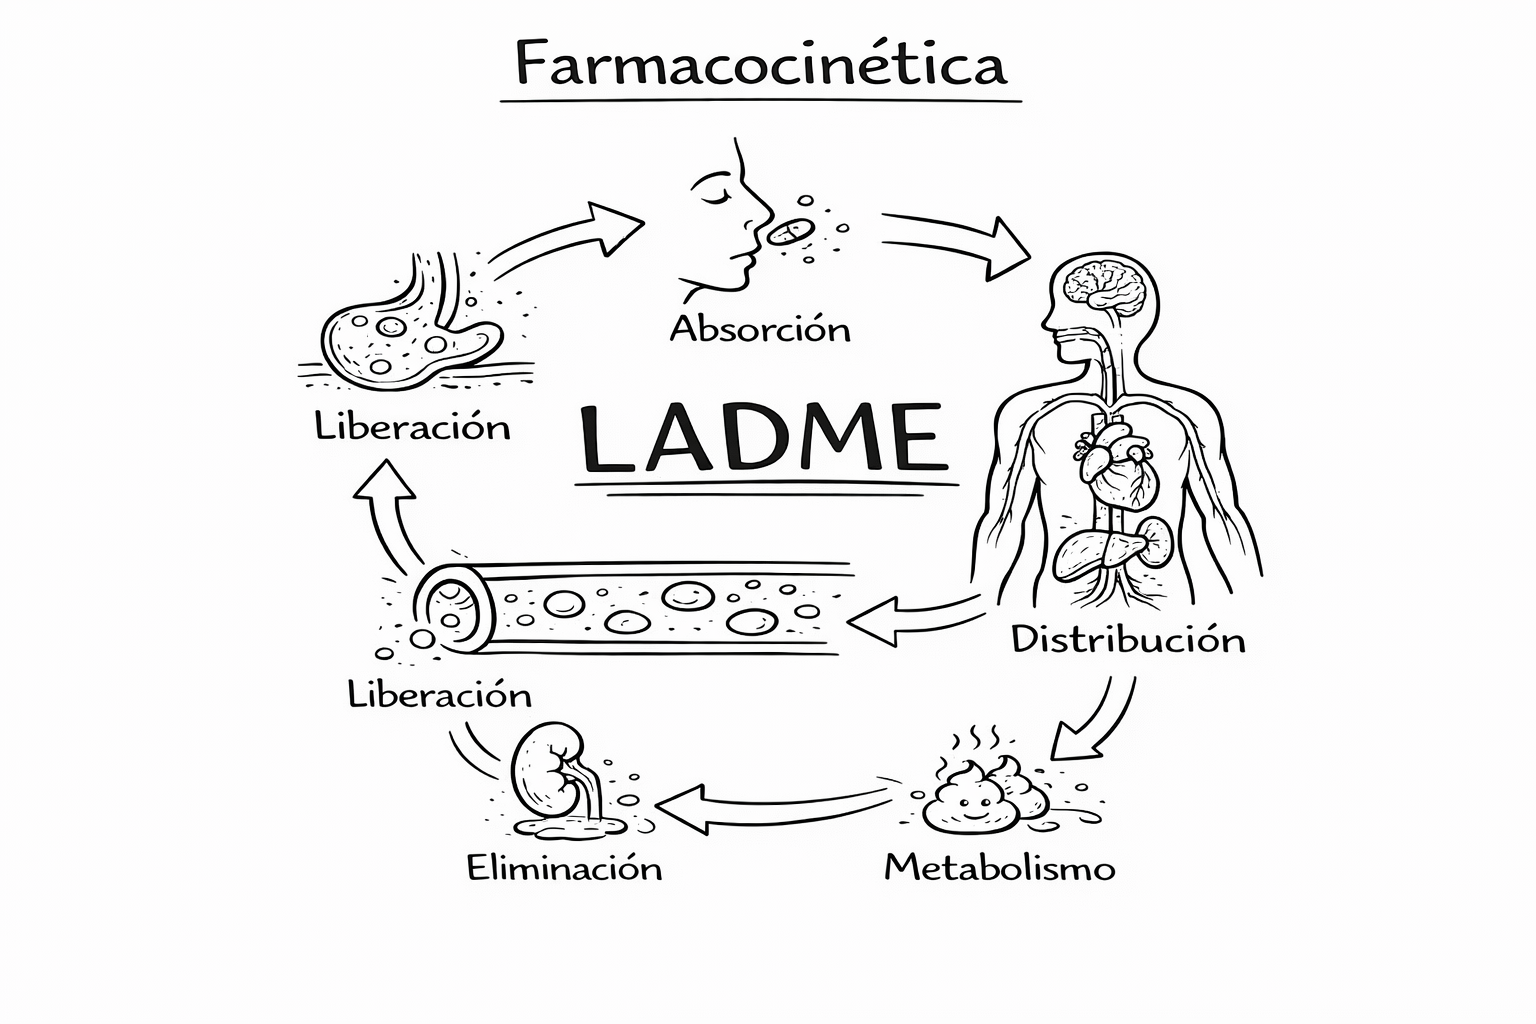
\includegraphics[scale=0.275]{LADME.png}
		\caption{Farmacocinética (LADME)}
	\end{figure}
	
	\subsection[Artículo 1. Vías de administración y velocidad de acción]{Artículo 1. Las vías de administración y la velocidad de acción}
	
	
	\momento{Planteo del tema} \\
	El análisis de la farmacocinética exige precisar cómo la vía de entrada de una sustancia psicoactiva (SPA) condiciona el tiempo de latencia y la intensidad de sus efectos en el Sistema Nervioso Central (SNC). Existe una tendencia en la divulgación preventiva a establecer comparaciones lineales y absolutas entre la vía inhalada (fumada) y la vía intravenosa (inyectada), afirmando categóricamente que la primera es siempre más rápida que la segunda. Sin embargo, la evidencia clínica contemporánea advierte que esta afirmación constituye una simplificación excesiva de un fenómeno condicionado por variables fisiológicas y por la cinética del pico plasmático, un matiz que el manual debe incorporar para evitar presentar como datos firmes lo que en la ciencia médica es una discusión abierta y compleja.
	
	\momento{Pregunta central} \\
	¿Es correcto afirmar de forma absoluta que la vía fumada es más rápida que la inyección intravenosa, o debe la velocidad de acción interpretarse en función de la cinética del pico plasmático y las variables técnicas de administración?
	
	\momento{Posturas u objeciones existentes} \\
	\begin{itemize}
		\item \submomento{Objeción 1:} Parece que el manual debe sostener la primacía cronológica de la vía fumada (estimada popularmente en un rango de 7 a 10 segundos) frente a la vía intravenosa (estimada de 15 a 30 segundos), ya que esto resalta la peligrosidad de sustancias de combustión inmediata como el crack o la pasta base.
		\item \submomento{Objeción 2:} Parece que la inyección intravenosa, al saltarse las barreras de absorción e ingresar directamente al torrente sanguíneo, debería ser catalogada de forma unívoca como la vía de llegada más veloz al cerebro en todos los casos, anidando cualquier equiparación con la vía pulmonar.
	\end{itemize}
	
	\momento{Fundamento o criterio de discernimiento} \\
	El realismo científico y la precisión técnica son indispensables para fundamentar la autoridad del manual en el diálogo interdisciplinar. La farmacocinética no puede reducirse a una tabla estática de segundos fijos; debe comprenderse como una interacción dinámica entre la maquinaria biológica del sujeto y la formulación química de la sustancia (Tríada de Zinberg\marginnote{Cfr. art.~\ref{art:zinberg} (Juzgar, Brevísimo Glosario)}). La distinción clínicamente relevante no reside únicamente en la velocidad cronológica absoluta, sino en la morfología de la curva de concentración de la sustancia en la sangre.
	
	\momento{Tesis y desarrollo argumental}\\ \\
	Respondemos que calificar a la vía fumada como unívocamente más rápida que la intravenosa es un error de simplificación, y que ambas vías deben presentarse como rutas de velocidad extrema cuyos efectos se diferencian por la cinética de su pico plasmático a través de tres precisiones teóricas:
	\begin{enumerate}
		\item \textbf{Variabilidad de los rangos clínicos de la vía intravenosa:} Los tiempos que habitualmente se asignan a la vía intravenosa (15-30 segundos) representan el rango superior de las estimaciones analizadas en laboratorios. Abundantes fuentes clínicas reportan que la llegada de la sustancia al cerebro mediante inyección IV puede ocurrir en un lapso de 10 a 15 segundos, lo cual equipara de forma real —y en ocasiones supera— los tiempos de la vía inhalada.
		\item \textbf{Dependencia de factores mecánicos y fisiológicos en la inhalación:} La velocidad de absorción por los capilares pulmonares no es un valor constante. Esta dimensión depende directamente de la técnica de inhalación del usuario, su volumen pulmonar útil, la profundidad y retención de la bocanada de humo, así como de la temperatura de combustión de la sustancia. Por lo tanto, no se puede establecer una cifra fija aplicable a todos los sujetos.
		\item \textbf{La verdadera distinción: el \textit{onset} o pico de concentración plasmática:} Lo que la ciencia verifica no es que la vía fumada <<llegue antes>> en términos de tiempo absoluto, sino que produce un \textit{pico de concentración plasmática} mucho más abrupto y vertical (\textit{onset} más empinado). Al inhalar, la sustancia pasa directamente de los alveolos al ventrículo izquierdo del corazón y de ahí al cerebro, saltándose la circulación venosa sistémica. Esto genera una oleada química concentrada que impacta masivamente en los circuitos de recompensa, creando un refuerzo subjetivo (el <<subidón>> o \textit{rush}) de enorme potencia adictiva, un mecanismo morfológico muy distinto al de la inyección venosa, que se distribuye de manera más diluida en el retorno sanguíneo general antes de alcanzar el árbol arterial.
	\end{enumerate}
	
	\momento{Respuesta a las objeciones} \\
	\begin{enumerate}
		\item \submomento{A la primera:} Si bien es loable alertar sobre la severidad y el daño del crack o la pasta base, utilizar datos cronológicos inexactos debilita la credibilidad del texto. El manual resulta mucho más riguroso si explica que la peligrosidad de la vía fumada radica en la brusquedad con la que secuestra el sistema dopaminérgico debido a la verticalidad de su pico plasmático, y no en una carrera de segundos disputada con la vía inyectada.
		\item \submomento{A la segunda:} Aunque la inyección IV deposita la totalidad de la dosis en la sangre de forma inmediata, el circuito circulatorio venoso impone un recorrido físico que matiza la velocidad de llegada al tejido cerebral. Reconocer que la vía pulmonar puede competir en velocidad con la intravenosa debido a su acceso directo a la circulación arterial es un dato que permite comprender con mayor precisión el altísimo potencial adictivo de las sustancias fumadas y la urgencia clínica que su consumo representa.
	\end{enumerate}
	
	\subsection{Artículo 2: Acción activa del organismo para gestionar una sustancia psicoactiva: la farmacocinética}
	
	\momento{Planteo del tema: La respuesta biológica activa ante una SPA.}
	El encuentro entre el ser humano y una sustancia psicoactiva (SPA) no es una
	recepción pasiva de efectos alteradores. Por el contrario, el organismo humano
	posee una \textbf{inteligencia biológica} que se activa de forma inmediata ante
	la presencia de componentes foráneos para intentar recuperar su equilibrio
	interno. Este proceso no se limita al momento del efecto subjetivo, sino que
	abarca un recorrido complejo que va desde que la sustancia toca el organismo
	hasta que es completamente eliminada.
	
	\momento{Pregunta central: ¿Qué hace el organismo con una SPA?} Se cuestiona
	si el cuerpo es un recipiente pasivo que solo experimenta los efectos de la
	sustancia, o si por el contrario despliega una \textbf{actividad química propia}
	para gestionar su entrada, tránsito y salida.
	
	\momento{Posturas u objeciones existentes}
	
	\begin{enumerate}
		\def\labelenumi{\arabic{enumi}.}
		
		\item
		\textbf{Parece que el organismo no hace nada activamente}, sino que
		simplemente espera a que la sustancia pierda su fuerza química de manera
		natural o espontánea.
		
		\item
		\textbf{Parece que el proceso es igual para todas las personas},
		independientemente de su edad, estado físico o historial de consumo.
		
		\item
		\textbf{Parece que la sustancia se dirige únicamente al cerebro}, dado que
		se define por su efecto psicoactivo, sin afectar otros tejidos u órganos.
		
		\item
		\textbf{Parece que una vez que termina el efecto en el cerebro, el organismo
			ya ha concluido su labor}, asumiendo que la sustancia ha desaparecido por
		completo del sistema.
		
	\end{enumerate}
	
	\momento{Fundamento o criterio de discernimiento} La \textbf{farmacocinética}
	es la rama de la ciencia que estudia precisamente esta actividad: la forma en
	que el cuerpo gestiona la entrada, el tránsito y la salida de una sustancia.
	Se distingue de la \textbf{farmacodinámica}, que estudia el impacto de esa
	sustancia sobre el organismo. Desde el instante en que se ingiere una SPA, el
	organismo inicia un proceso secuencial e irreversible para procesarla y
	expulsarla, compuesto por cuatro etapas: \textbf{liberación, absorción,
		distribución y metabolismo-eliminación}.
	
	\momento{Tesis y desarrollo argumental}\\
	Respondemos que el organismo actúa como un \textbf{procesador químico activo}
	que busca defender su equilibrio interno ante cualquier estímulo que altere sus
	procesos fisiológicos. Este proceso se despliega en las siguientes etapas:
	
	\begin{itemize}
		
		
		\begin{figure}[h!]
			\centering
			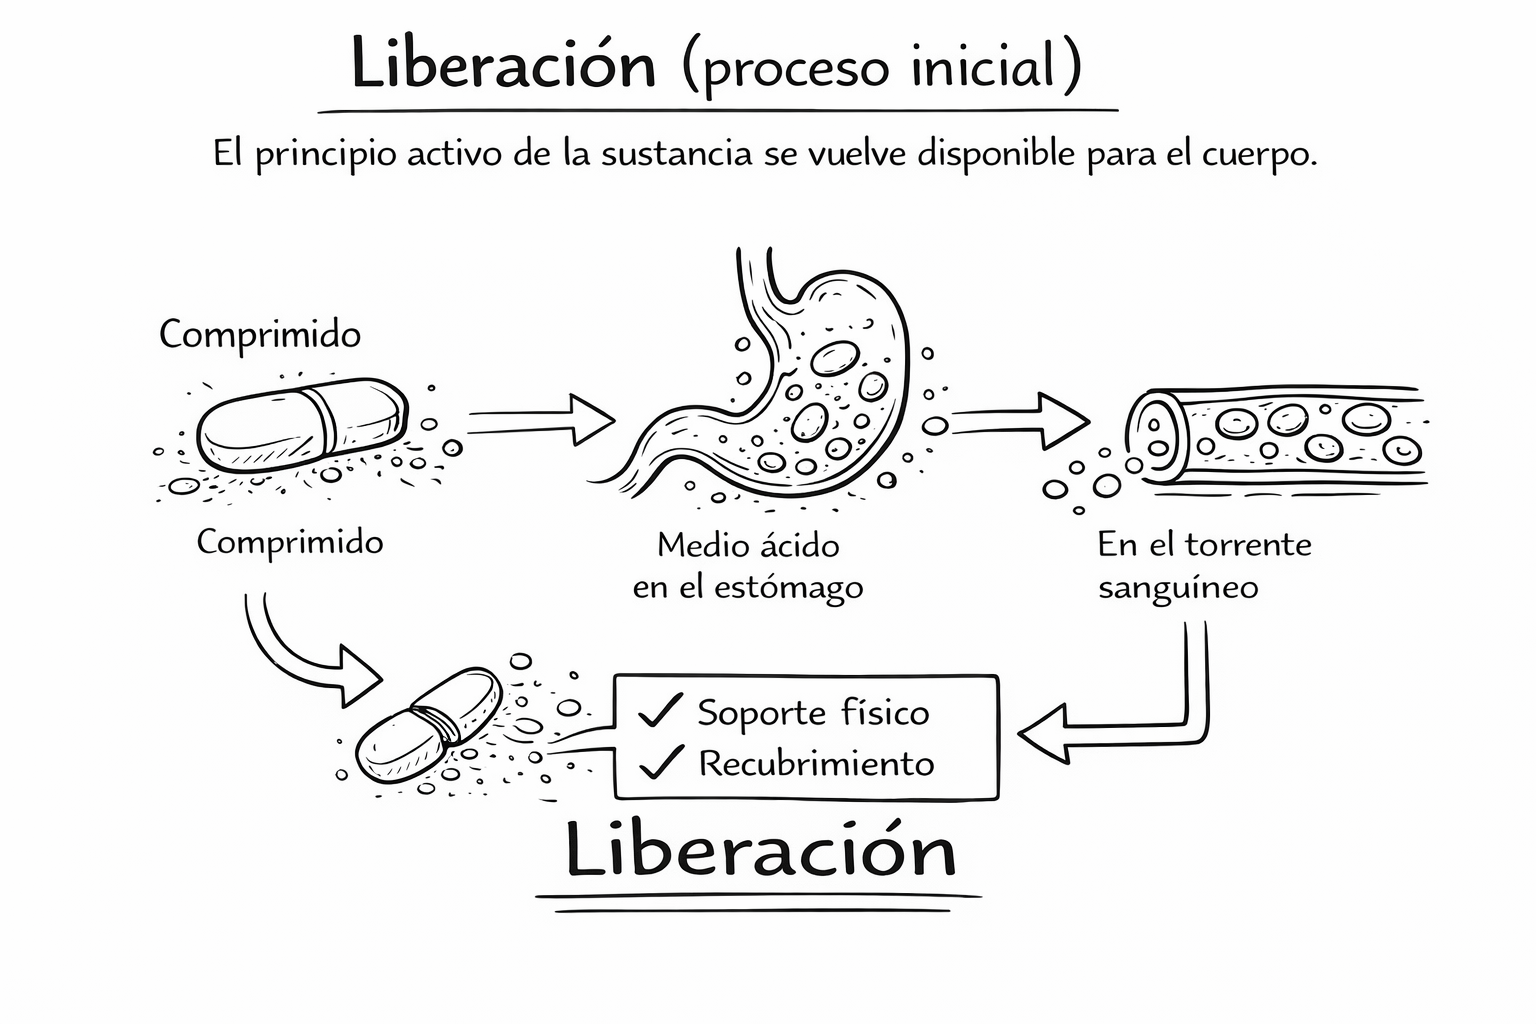
\includegraphics[scale=0.15]{liberación.png}
			\caption{Liberación}
		\end{figure}
		
		\item
		\textbf{Liberación:} Es la fase inicial en la que el principio activo de la
		SPA se separa de su soporte físico (comprimido, humo, polvo) para quedar en
		un estado molecular que el cuerpo pueda absorber. La velocidad de esta
		liberación es determinante: una liberación instantánea —como ocurre al
		fumar— genera un impacto cerebral máximo y un mayor potencial adictivo; una
		liberación lenta —como la de un parche— reduce ese efecto reforzador.
		
		\begin{figure}[h!]
			\centering
			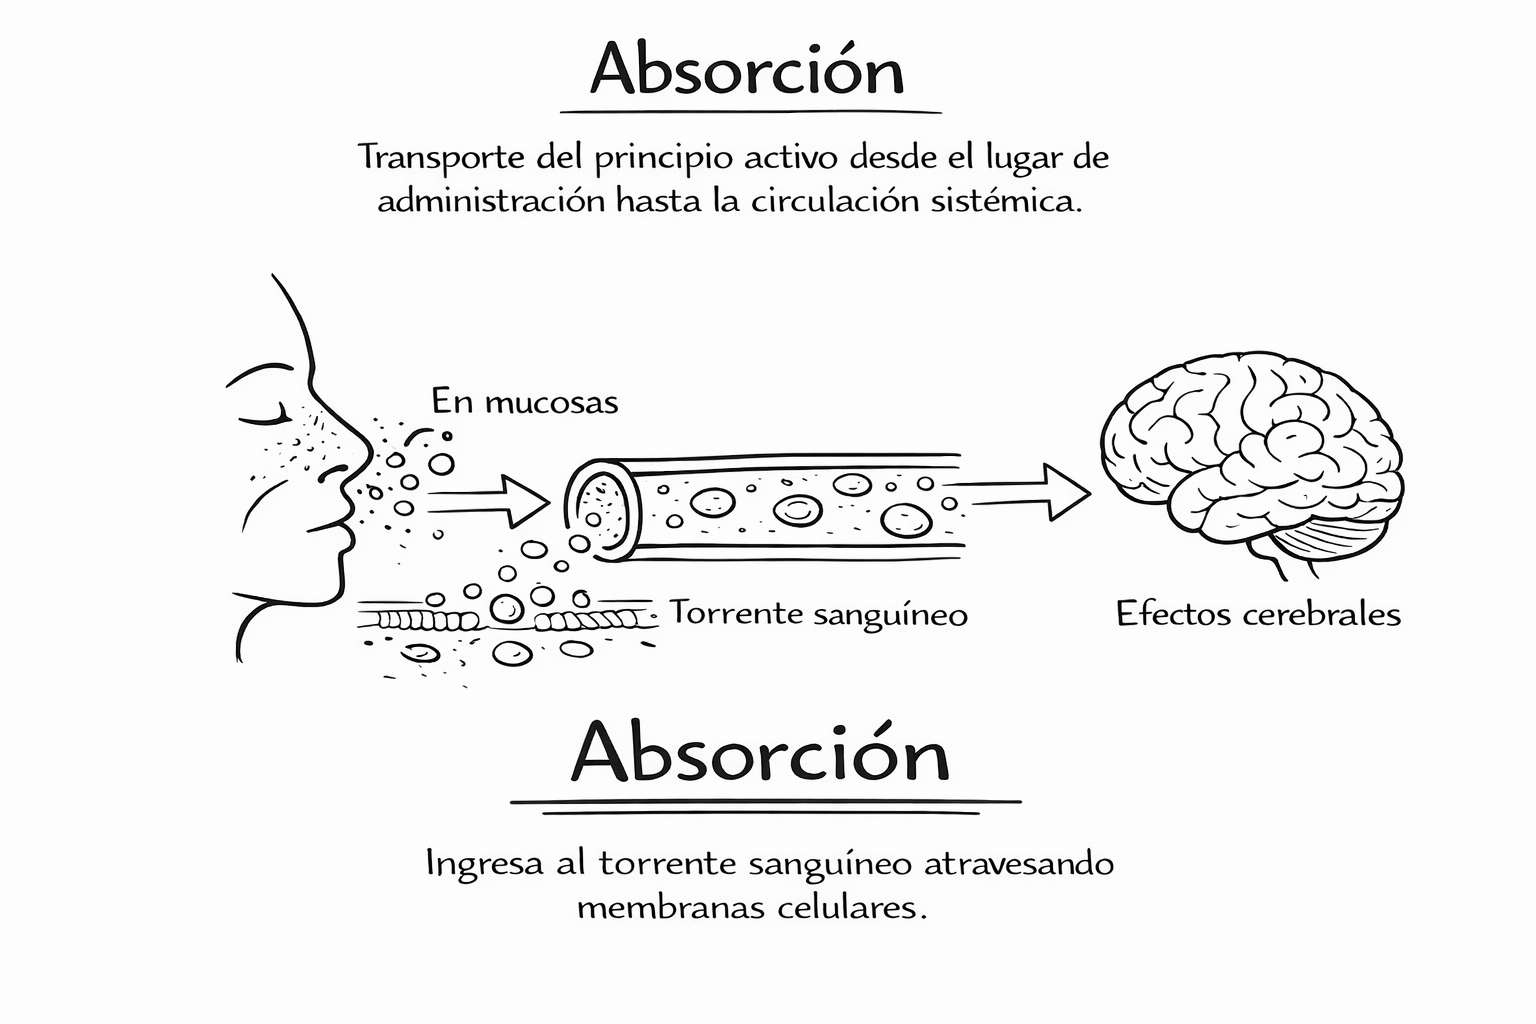
\includegraphics[scale=0.15]{absorción.png}
			\caption{Absorción}
		\end{figure}
		
		\item
		\textbf{Absorción:} Es el proceso por el cual el principio activo atraviesa
		las membranas celulares para ingresar al torrente sanguíneo. La vía de
		administración es el factor externo más determinante: fumar permite una
		absorción en 7 a 10 segundos a través de los alvéolos pulmonares, mientras
		que la vía oral puede tardar entre 20 y 30 minutos debido al tránsito
		digestivo. La edad, el historial de consumo y las propiedades químicas de la
		sustancia condicionan también la eficacia de este proceso.
		
		\begin{figure}[h!]
			\centering
			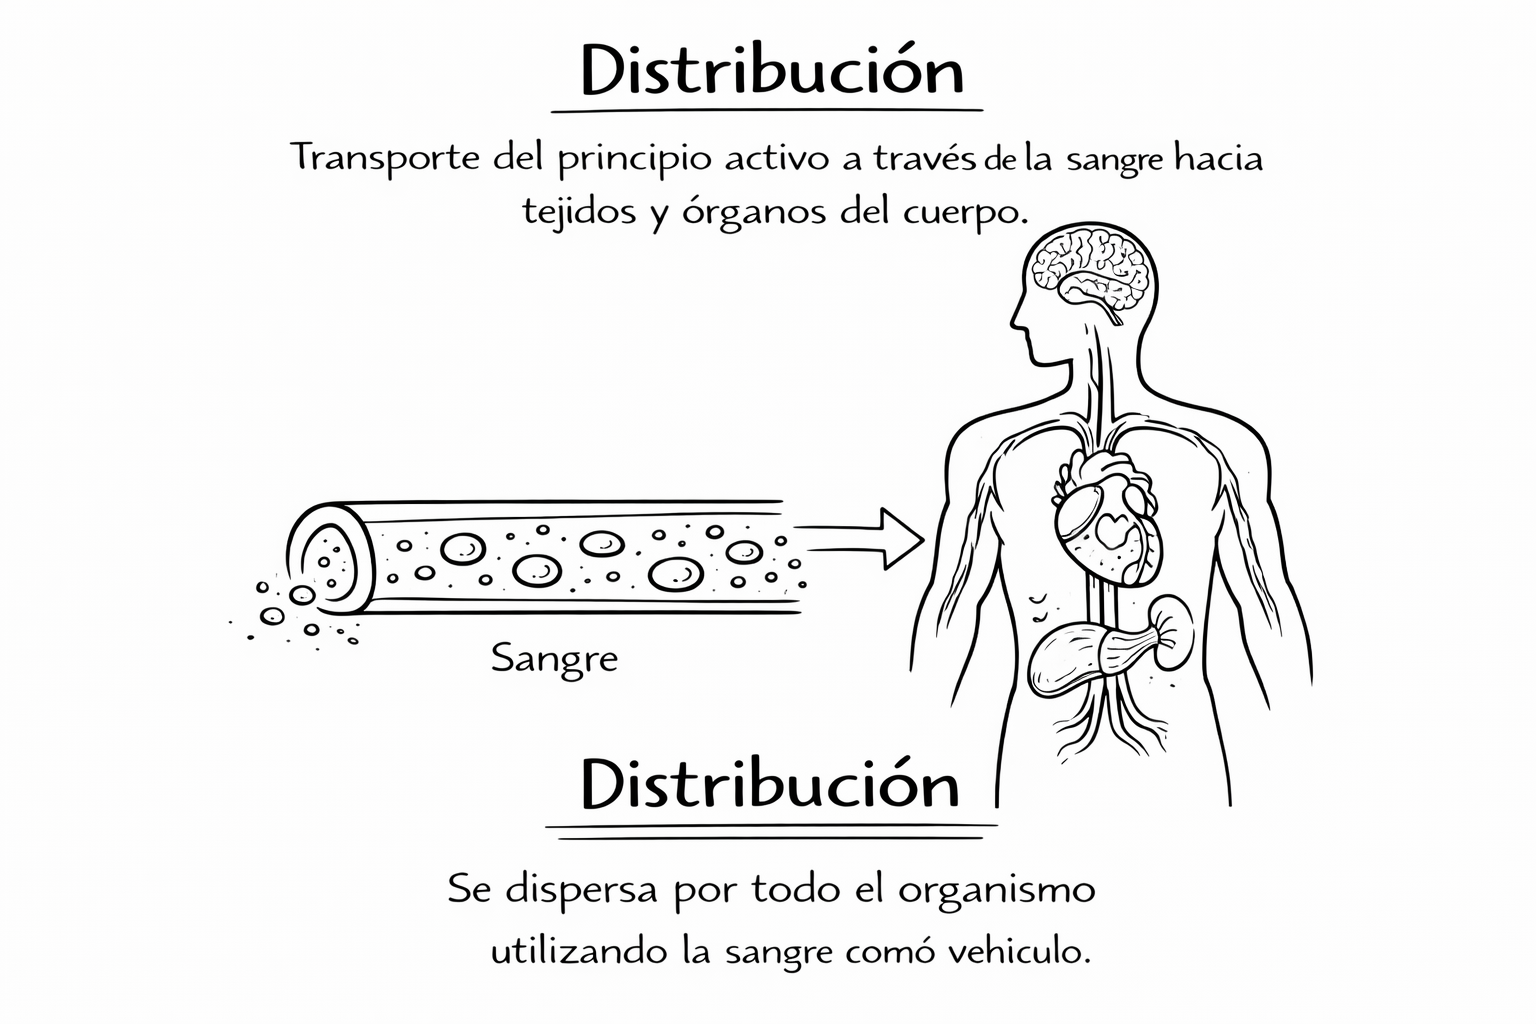
\includegraphics[scale=0.15]{distribución.png}
			\caption{Distribución}
		\end{figure}
		
		\item
		\textbf{Distribución:} Una vez en la sangre, la sustancia no permanece
		estática ni se dirige exclusivamente al cerebro. El sistema circulatorio la
		transporta hacia diversos tejidos y órganos —hígado, riñones, tejido
		adiposo— según la afinidad química de cada molécula. Esta acción sistémica
		explica que las consecuencias del consumo no sean solo neurológicas, sino que
		afecten al organismo en su conjunto.
		
		
		\item
		\textbf{Barrera hematoencefálica y acceso al cerebro:} Para alcanzar el
		tejido neuronal, la SPA debe atravesar la \textbf{barrera hematoencefálica
			(BHE)}, una membrana protectora de células fuertemente unidas que filtra
		selectivamente los componentes del torrente sanguíneo. Solo pueden cruzarla
		sustancias con \textbf{molécula pequeña} y \textbf{liposolubilidad}
		(solubilidad en grasas). Esta es precisamente la característica que define a
		las SPA: su capacidad para atravesar esta frontera biológica e interferir
		directamente en la comunicación entre neuronas. Una vez dentro, se depositan
		en el tejido adiposo, lo que explica por qué el organismo puede permanecer
		impregnado de ellas mucho tiempo después del consumo.
		
		\item
		\textbf{Metabolismo y eliminación:} Una vez que la SPA ha cumplido su	recorrido, el organismo inicia el proceso de neutralizarla y expulsarla.
		El \textbf{hígado} es el principal órgano metabolizador: transforma
		químicamente la sustancia en metabolitos menos activos o inactivos que
		puedan ser eliminados. La expulsión final se produce principalmente a
		través de los \textbf{riñones} (orina), aunque también intervienen el
		sudor, la bilis y el aire exhalado. La velocidad de este proceso depende
		de la naturaleza química de la sustancia, la edad del individuo y el
		estado de sus órganos. El uso repetido puede sobrecargar estos sistemas,
		deteriorando progresivamente su capacidad de respuesta.
		
		
		\item
		\textbf{Metabolismo y eliminación:} Una vez que la SPA ha cumplido su recorrido, el organismo inicia el proceso de neutralizarla y expulsarla. El hígado es el principal órgano metabolizador: transforma químicamente la sustancia en metabolitos menos activos o inactivos que puedan ser eliminados. La expulsión final se produce principalmente a través de los riñones (orina), aunque también intervienen el sudor, la bilis y el aire exhalado. Para medir el tiempo de este proceso	se utiliza el concepto de \textbf{vida media}: el período que el organismo necesita para eliminar la mitad de la dosis original, dato que determina tanto la duración de los efectos como el tiempo real de desintoxicación. Este proceso no es uniforme: los niños y adultos mayores metabolizan más lentamente, el uso repetido puede sobrecargar el hígado y los riñones deteriorando su capacidad de respuesta, y la variable del sexo es especialmente crítica, ya que la mayor proporción de tejido adiposo en la mujer ralentiza la eliminación total, exigiendo procesos de desintoxicación más prolongados.
		
	\end{itemize}
	
	\momento{Respuesta a las objeciones}
	
	\begin{enumerate}
		\def\labelenumi{\arabic{enumi}.}
		
		\item
		\submomento{A la primera objeción:} El organismo no es pasivo. El metabolismo
		es un \textbf{proceso químico complejo y constante} que convierte las
		sustancias en desechos para ser eliminados a través de diversos fluidos y
		vías corporales. El cuerpo trabaja activamente desde el primer momento de
		contacto con la SPA.
		
		\item
		\submomento{A la segunda objeción:} El proceso varía significativamente según
		el perfil del individuo. Factores como la \textbf{edad} —niños y adultos
		mayores procesan más lento—, el \textbf{historial de consumo} y la
		\textbf{vulnerabilidad biológica} determinan la eficacia con que el cuerpo
		absorbe, distribuye y elimina la sustancia.
		
		\item
		\submomento{A la tercera objeción:} Aunque el efecto buscado sea cerebral, la
		farmacología demuestra que las SPA se distribuyen por múltiples órganos
		durante su tránsito, lo que explica las consecuencias físicas y médicas del
		consumo prolongado más allá del sistema nervioso central.
		
		
		\item
		\textbf{A la cuarta objeción:} El cese del efecto mental no implica la
		limpieza total del organismo. El metabolismo y la eliminación son procesos
		que demandan tiempo y dependen del estado del hígado y los riñones. El
		cuerpo puede permanecer \textbf{impregnado de la sustancia} en el tejido
		adiposo durante un tiempo prolongado, lo que exige procesos de
		desintoxicación que van mucho más allá de la desaparición subjetiva de
		los efectos.
		
	\end{enumerate}
	
	\subsection{Artículo 3: La liposolubilidad como factor crítico en el almacenamiento de drogas}
	
	\momento{Planteo del tema: La afinidad química y la permanencia orgánica} El estudio de la farmacocinética revela que el impacto de una sustancia no depende únicamente de su potencia, sino de su capacidad para integrarse en los tejidos del huésped. La estructura molecular de las sustancias psicoactivas (SPA) define si estas simplemente circulan por el torrente sanguíneo o si encuentran refugio en las reservas lipídicas del cuerpo, extendiendo su presencia biológica mucho más allá de la desaparición de los efectos psíquicos inmediatos.
	
	\momento{Pregunta central: ¿Qué significa que una sustancia sea liposoluble y por qué es un factor crítico en el almacenamiento de drogas en el cuerpo?} Se cuestiona si la solubilidad es un mero detalle técnico del laboratorio o si es la causa fundamental de la dificultad para lograr una desintoxicación total y de las diferencias biológicas en los procesos de recuperación entre varones y mujeres.
	
	\momento{Posturas u objeciones existentes}
	
	\begin{enumerate}
		\def\labelenumi{\arabic{enumi}.}
		
		\item
		\textbf{Parece que las drogas se eliminan por completo del cuerpo en pocos días,} ya que los efectos mentales de euforia o sedación suelen durar apenas unas horas.
		
		\item
		\textbf{Parece que la grasa corporal es un tejido inerte} que no tiene relación con el proceso de la adicción, el cual se asocia comúnmente solo al cerebro o a la sangre.
		\item
		\textbf{Parece que el metabolismo y almacenamiento de sustancias es idéntico para todos los seres humanos}, sin que el género o la composición física del individuo alteren la velocidad de limpieza orgánica.
	\end{enumerate}
	
	\momento{Fundamento o criterio de discernimiento} Sin embargo, contra esto, la ciencia enseña que \textbf{la mayoría de las sustancias psicoactivas son liposolubles}, lo que significa que tienen la propiedad de disolverse fácilmente en grasas. Este criterio es esencial para comprender cómo las SPA atraviesan defensas biológicas que otros fármacos no pueden cruzar y cómo logran permanecer <<impregnadas>> en el organismo.
	
	\momento{Tesis y desarrollo argumental}\\ Respondemos que la \textbf{liposolubilidad} es la característica molecular que permite a una sustancia atravesar las membranas celulares compuestas por lípidos, siendo el factor crítico en el almacenamiento por las siguientes razones biológicas:
	
	\begin{itemize}
		
		\item
		\textbf{Acceso al cerebro:} Al ser solubles en grasa, estas sustancias pueden cruzar la \textbf{barrera hematoencefálica}, una membrana protectora que bloquea a los medicamentos hidrosolubles (como los antibióticos) pero permite el paso de moléculas pequeñas y liposolubles, dándoles acceso directo a las neuronas.
		\item
		\textbf{Depósito en el tejido adiposo:} Las SPA no permanecen únicamente en la sangre; debido a su afinidad química, se depositan en el \textbf{tejido adiposo (grasa)} que rodea los órganos y las venas.
		\item
		\textbf{Diferenciación por género:} El cuerpo de la \textbf{mujer} está rodeado de tejido adiposo de forma sistémica, mientras que en los hombres se concentra principalmente en el vientre y la espalda. Por ello, las sustancias permanecen \textbf{más tiempo impregnadas en las mujeres}, dificultando su desintoxicación y recuperación en comparación con los varones.
		\item
		\textbf{Fenómeno de re-liberación:} La grasa actúa como un reservorio que mantiene la sustancia guardada; ante estímulos como el \textbf{calor intenso o la movilización de grasas}, el cuerpo puede liberar estos residuos de vuelta al torrente sanguíneo incluso meses después del último consumo.
	\end{itemize}
	
	\momento{Respuesta a las objeciones}
	
	\begin{enumerate}
		\def\labelenumi{\arabic{enumi}.}
		
		\item
		\submomento{A la primera objeción:} Aunque los efectos mentales desaparecen, la sustancia sigue presente. Una desintoxicación de pocos días solo limpia la sangre, pero no logra eliminar la droga acumulada en el sistema adiposo, lo que requiere procesos de recuperación más prolongados.
		
		\item
		\submomento{A la segunda objeción:} La grasa es un actor dinámico en la adicción. El fenómeno del <<viaje seco>> demuestra que la sustancia almacenada en el tejido adiposo puede reaparecer en la sangre meses después, provocando síntomas de consumo sin haber ingerido la droga nuevamente.
		\item
		\submomento{A la tercera objeción:} El almacenamiento es desigual. Debido a que las SPA son liposolubles, la mayor proporción de grasa corporal en las mujeres las vuelve biológicamente más susceptibles a una impregnación profunda y duradera, lo que demanda estrategias de tratamiento con perspectiva de género.
	\end{enumerate}
	
	\subsection{Artículo 4: La liposolubilidad de las sustancias y el fenómeno del \textit{viaje seco}: entre la persistencia biológica y el condicionamiento psíquico}
	
	\momento{Planteo del tema} \\
	El análisis de la farmacocinética exige precisar cómo ciertas sustancias psicoactivas (SPA) se almacenan en el organismo debido a su afinidad con los tejidos grasos. Es frecuente escuchar en los dispositivos territoriales la descripción del \textit{viaje seco} o \textit{flashback}, definido popularmente como la reaparición repentina de los efectos psicoactivos meses después de haber suspendido el consumo, atribuyéndolo de forma categórica a la liberación de la sustancia acumulada en el tejido adiposo. Si bien la liposolubilidad es un hecho científico incuestionable, la afirmación de que su liberación desde la grasa produzca efectos clínicos significativos carece de consenso absoluto. Resulta necesario juzgar cómo presentar este fenómeno con la debida cautela científica, evitando proponer como certezas firmes lo que en la medicina actual constituye una hipótesis en revisión.
	
	\momento{Pregunta central} \\
	¿Debe el manual presentar la re-liberación de sustancias desde el tejido adiposo como la causa probada y definitiva del \textit{viaje seco}, o corresponde situar este fenómeno dentro de un modelo multifactorial que contemple la sensibilización de receptores y el condicionamiento psicológico?
	
	\momento{Posturas u objeciones existentes} \\
	\begin{itemize}
		\item \submomento{Objeción 1:} Parece que el manual debe sostener con firmeza que el \textit{viaje seco} está causado directamente por la grasa acumulada que se libera meses después (por ejemplo, durante el ejercicio físico o la pérdida de peso), ya que esto ofrece una explicación biológica simple y de fuerte impacto pedagógico para alertar sobre la persistencia orgánica del daño.
		\item \submomento{Objeción 2:} Parece que relativizar la causa biológica del \textit{flashback} reduciría el fenómeno a una mera sugestión psicológica o espiritual del sujeto, desestimando la base material del sufrimiento que experimenta el hermano en recuperación.
	\end{itemize}
	
	\momento{Fundamento o criterio de discernimiento} \\
	La honestidad intelectual y el realismo científico son virtudes pastorales que protegen la autoridad del manual. Presentar con certeza absoluta un mecanismo biológico debatido debilita la fundamentación técnica del texto ante la academia. El discernimiento nos invita a reconocer que la fragilidad del ser humano es integral; las huellas que deja el consumo no se limitan a un depósito de grasa inerte, sino que configuran complejas redes de memoria en el sistema nervioso y en la psiquis, las cuales interactúan dinámicamente con el contexto.
	
	\momento{Tesis y desarrollo argumental}\\ \\
	Respondemos que, si bien la liposolubilidad y el depósito en el tejido adiposo son datos farmacológicos firmes (especialmente notorios en sustancias como el cannabis), la afirmación de que la re-liberación desde la grasa genere efectos psicoactivos clínicamente relevantes meses después debe presentarse con cautela, integrando otros mecanismos contemporáneos a través de tres precisiones teóricas:
	\begin{enumerate}
		\item \textbf{El carácter subclínico de la re-liberación lipídica:} La evidencia clínica actual advierte que, si bien durante procesos metabólicos como la lipólisis (pérdida de peso o ejercicio intenso) se liberan trazas de la sustancia acumulada en la grasa hacia el torrente sanguíneo, los niveles alcanzados son generalmente subclínicos. Esto significa que las concentraciones resultantes se ubican muy por debajo del umbral necesario para reactivar de forma masiva los efectos psicoactivos originales en el tejido cerebral.
		\item \textbf{La sensibilización de receptores en el Sistema Nervioso:} El fenómeno de los \textit{flashbacks} —común en trayectorias vinculadas a alucinógenos como el LSD y otras SPA— encuentra una explicación mucho más sólida en la neuroplasticidad\marginnote{Cfr. art.~\ref{art:neuroplasticidad} (Juzgar, Brevísimo Glosario)} desadaptativa. El consumo crónico genera una hipersensibilidad o alteración persistente en los receptores neuronales. Ante determinados estímulos estresantes o fatiga extrema, estos receptores pueden activarse de forma anómala, evocando parcialmente la percepción del consumo sin necesidad de que la sustancia esté físicamente circulando en el organismo.
		\item \textbf{La potencia del condicionamiento psicológico y ambiental:} El marco de la Tríada de Zinberg\marginnote{Cfr. art.~\ref{art:zinberg} (Juzgar, Brevísimo Glosario)} (sujeto-sustancia-contexto) recuerda que los estímulos ambientales operan sobre la memoria afectiva. El regreso a las esquinas de consumo, un aroma, una música o un estado de angustia existencial similar al que precedía a la intoxicación pueden gatillar una respuesta psicofisiológica que simule el efecto de la droga. La mente y el corazón del hermano, condicionados por el hábito pasado, reviven la experiencia debido a la profundidad del patrón de aprendizaje almacenado.
	\end{enumerate}
	
	\momento{Respuesta a las objeciones} \\
	\begin{enumerate}
		\item \submomento{A la primera:} La rigurosidad del manual no disminuye su fuerza preventiva. Es mucho más profundo explicar a las comunidades y a las carteras del Estado que la adicción modifica las estructuras de la percepción y los centros de alerta psíquica del individuo (haciéndolo vulnerable a revivir el viaje a través de disparadores ambientales), que sostener una teoría puramente mecánica sobre la grasa corporal que la ciencia clínica califica como controvertida o débil.
		\item \submomento{A la segunda:} Atribuir el \textit{viaje seco} a la sensibilización de receptores y al condicionamiento no resta gravedad al fenómeno ni lo vuelve una ilusión. Al contrario, fundamenta neurobiológica y psicológicamente el porqué un hermano que lleva meses sin consumir puede sufrir crisis repentinas al habitar el mismo territorio de desprotección. Esto justifica la necesidad de una pastoral que cure la orfandad a través del enraizamiento, proveyendo un entorno seguro y una familia comunitaria estables donde la memoria afectiva pueda comenzar a sanar.
	\end{enumerate}
	
	
	\newpage
	
	\section{La farmacodinámica. El impacto de la sustancia en el organismo}
	
	Si en la sección anterior analizamos la farmacocinética (el camino de la sustancia y la reacción del cuerpo ante ella), la farmacodinámica se enfoca en el \textbf{impacto estructural y funcional} que el componente químico genera al infiltrarse en el sistema nervioso central. En esta etapa, la sustancia deja de ser un pasajero en el torrente sanguíneo para convertirse en un agente activo que altera la comunicación más íntima de nuestras células
	
	\subsection{Artículo 1: El sistema de recompensa y la ilusión del deseo: más allá de la \textit{molécula del placer}}
	
	\momento{Planteo del tema} \\
	La descripción tradicional del circuito de recompensa mesolímbico suele identificar a la dopamina\label{art:dopamina} de manera casi exclusiva como la \textit{molécula del placer}, reduciendo el engranaje neurobiológico a una mera búsqueda de gratificación hedónica. Sin embargo, la neurociencia contemporánea ha superado significativamente esta lectura reduccionista. La evidencia clínica actual demuestra que el sistema dopaminérgico no media el disfrute o goce real de la sustancia, sino los mecanismos de anticipación, motivación y asignación de importancia ante los estímulos ambientales. Resulta indispensable juzgar cómo presentar este circuito sin caer en simplificaciones conceptuales, permitiendo que el manual comprenda la verdadera anatomía del deseo desordenado.
	
	\momento{Pregunta central} \\
	¿De qué manera debe definirse el circuito dopaminérgico mesolímbico: como el sistema del placer hedónico o como el motor de la saliencia motivacional y el querer compulsivo?
	
	\momento{Posturas u objeciones existentes} \\
	\begin{itemize}
		\item \submomento{Objeción 1:} Parece que el manual debe sostener la definición popular de la dopamina como la molécula del placer, dado que esto simplifica la pedagogía preventiva y permite denunciar con mayor facilidad la trampa hedonista que propone el mercado de consumo.
		\item \submomento{Objeción 2:} Parece que la distinción entre los mecanismos químicos del deseo y los del disfrute real es un detalle técnico accesorio que no aporta valor sustancial al discernimiento pastoral y espiritual del agente territorial.
	\end{itemize}
	
	\momento{Fundamento o criterio de discernimiento}
	
	\marginnote{Cfr. La adicción como búsqueda espiritual fallida (cap. 7)}
	
	El realismo antropológico y la visión tomista de las pasiones enseñan que el ser humano posee un apetito concupiscible que puede descarrilarse, obsesionándose con la captura de un objeto (un querer ciego) incluso cuando este ha dejado de saciar o reportar deleite auténtico al alma. Esta disociación científica se alinea perfectamente con el concepto de \textit{esclavitud química} expuesto por el Magisterio de la Iglesia, donde la voluntad queda encadenada a la búsqueda de un ídolo que ya no ofrece consuelo sino desolación.
	
	\momento{Tesis y desarrollo argumental}\\ \\
	Respondemos que el circuito mesolímbico debe presentarse como un sistema de saliencia motivacional y no como un mero termómetro de placer, distinguiendo con claridad entre la fuerza del impulso por conseguir la sustancia (\textit{wanting}) y el agrado hedónico real de su consumo (\textit{liking}), a través de tres dimensiones teóricas:
	\begin{enumerate}
		\item \textbf{La dopamina como motor de la anticipación:} La neurociencia actual verifica que la liberación masiva de dopamina ocurre ante la expectativa del consumo y la preparación de la conducta de búsqueda. No es la sustancia en sí la que genera la mayor oleada dopaminérgica, sino las señales del entorno que anuncian su llegada, operando como un motor de fijación atencional.
		
		\item \textbf{La disociación entre el querer y el gustar:} Los procesos de deleite y goce hedónico (\textit{liking}) están mediados en el organismo por sistemas neuroquímicos distintos, vinculados a los opioides endógenos y los endocannabinoides. En el trastorno por uso de sustancias (TUS), el circuito del agrado se desgasta rápidamente por habituación, mientras que el circuito dopaminérgico del querer compulsivo (\textit{wanting}) se hipertrofia, atrapando al sujeto en un bucle de persecución ansiosa.
		
		\item \textbf{El secuestro de la saliencia motivacional:} El circuito mesolímbico funciona originalmente como un asignador de relevancia que le dice al individuo qué estímulos son vitales para su supervivencia como el alimento, la hidratación o el encuentro social. El consumo crónico altera este mecanismo de evaluación, provocando que el cerebro asigne una importancia máxima y deformada a la sustancia, subordinando de forma trágica las necesidades fundamentales del ser social.
	\end{enumerate}
	
	\momento{Respuesta a las objeciones} \\
	\begin{enumerate}
		\item \submomento{A la primera:} Reducir la adicción al placer debilita la denuncia contra el consumismo. El relato del mercado afirma que el consumo es igual a la felicidad; explicar que la neurobiología desmonta esa ilusión demostrando que la adicción es un \textit{querer sin disfrutar} desenmascara la falsedad de los paraísos artificiales de forma mucho más contundente para la prevención comunitaria.
		\item \submomento{A la segunda:} Lejos de ser un tecnicismo vacío, esta distinción enriquece el juicio pastoral. Permite al agente comprender que el hermano atrapado en el consumo no es un buscador de placer inmoral, sino una persona cuya brújula motivacional interna ha sido secuestrada, requiriendo el andamiaje de un amor responsable en comunidad para recuperar su libertad original.
	\end{enumerate}

	\subsection{Artículo 2: Interacción directa de la molécula con la maquinaria biológica}
	
	\momento{Planteo del tema: La acción de la sustancia sobre la biología}. Una vez que la sustancia ha recorrido el camino de la absorción y distribución, entramos en la dimensión de lo que el componente químico le hace al cuerpo. Mientras que la farmacocinética se ocupa del <<tránsito>>, este nuevo campo analiza la interacción directa entre la molécula externa y la maquinaria biológica del ser humano, centrando su atención en cómo se altera la comunicación más íntima de nuestras células.
	
	\momento{Pregunta central: ¿Qué hace una sustancia psicoactiva (SPA) con el organismo?} Se cuestiona si la sustancia es un agente que simplemente produce sensaciones pasajeras o si posee la capacidad de intervenir y modificar de manera estructural y funcional la operación natural de los sistemas biológicos y órganos del sujeto.
	
	\momento{Posturas u objeciones existentes}
	
	\begin{enumerate}
		\def\labelenumi{\arabic{enumi}.}
		
		\item
		\textbf{Parece que la SPA solo afecta la voluntad o el carácter}, sugiriendo que el efecto es meramente conductual y que el organismo permanece biológicamente igual antes y después del consumo.
		
		\item
		\textbf{Parece que el efecto se limita exclusivamente al cerebro}, ignorando que el cuerpo es una unidad y que la sustancia circula por todo el torrente sanguíneo hacia otros tejidos.
		\item
		\textbf{Parece que la sustancia actúa de forma aislada}, como si no interactuara con las señales químicas naturales que el cuerpo ya posee para su supervivencia.
	\end{enumerate}
	
	\momento{Fundamento o criterio de discernimiento} Sin embargo, contra esto, las sustancias psicoactivas son componentes que \textbf{afectan el funcionamiento del sistema nervioso central (SNC)} y tienen la capacidad de \textbf{alterar los procesos bioquímicos de los tejidos y órganos del cuerpo}. Este impacto no es superficial, sino que interfiere con la forma en que las células se comunican y procesan la información necesaria para la vida.
	
	\momento{Tesis y desarrollo argumental}\\ Respondemos que una SPA actúa sobre el organismo interfiriendo en la comunicación neuronal y alterando la homeostasis (equilibrio dinámico) de diversos sistemas orgánicos. Este proceso se desarrolla a través de tres mecanismos fundamentales:
	
	\begin{itemize}
		
		\item
		\textbf{La imitación química (El <<impostor>>):} Sustancias como los cannabinoides o los opioides poseen una estructura química similar a la de los neurotransmisores naturales. Gracias a esta \textbf{llave de acción} (complementariedad estructural), engañan a los receptores y se adhieren a las neuronas para activarlas; sin embargo, al ser <<llaves falsas>>, provocan el envío de mensajes anormales que el cerebro no puede regular
		\item
		\textbf{La interferencia en el reciclaje (La <<inundación>>):} Estimulantes como la cocaína actúan sobre los transportadores encargados de la \textbf{recaptación} (el reciclaje químico). Al bloquear este proceso, impiden que la dopamina\marginnote{Cfr. art.~\ref{art:dopamina} (Juzgar, Las sustancias y el organismo, La farmacodinámica..., Art. 1...)} regrese a su neurona de origen, causando que el espacio intersináptico se \textbf{inunde} y los receptores se saturen de forma anormal, forzando al cerebro a adaptarse a niveles de estimulación no naturales.
		\item
		\textbf{Impacto sistémico y bioquímico:} Más allá del cerebro, la farmacología demuestra que las SPA alteran los procesos bioquímicos de otros órganos. El consumo abundante debilita el \textbf{sistema inmunológico}, volviendo al sujeto más susceptible a infecciones y afectando directamente funciones en el hígado y los riñones debido a la toxicidad de los componentes y sus adulterantes.
	\end{itemize}
	
	\momento{Respuesta a las objeciones}
	
	\begin{enumerate}
		\def\labelenumi{\arabic{enumi}.}
		
		\item
		\submomento{A la primera objeción:} La acción de la sustancia no es solo moral o conductual; existen \textbf{cambios biológicos visibles} e indicadores físicos (signos) como la alteración de la frecuencia cardíaca, cambios en la actividad cerebral captados en el diagnóstico por imágenes, y daños en tejidos específicos.
		
		\item
		\submomento{A la segunda objeción:} Aunque su nombre enfatice la <<psicoactividad>> (cerebro), la sustancia se distribuye por todo el organismo. Produce consecuencias médicas sistémicas que incluyen enfermedades cardiovasculares, respiratorias, renales y hepáticas, demostrando que \textbf{el cuerpo es una unidad} que sufre el impacto de forma integral.
		\item
		\submomento{A la tercera objeción:} Las SPA no trabajan en el vacío. Utilizan su \textbf{llave de acción} para infiltrarse en el lenguaje químico natural del cuerpo y secuestrar la maquinaria existente (receptores). Al enviar mensajes anormales a través de la red neuronal, desequilibran las funciones vitales que el organismo realiza de forma autónoma para su supervivencia
	\end{enumerate}
	
	\subsection{Artículo 3: Sobre la definición de la adicción: entre el modelo neurobiológico y la integridad del sujeto}
	
	\momento{Planteo del tema} El estudio de la farmacodinámica y el impacto de las sustancias en el organismo suele apoyarse de forma predominante en el modelo del National Institute on Drug Abuse (NIDA), el cual define la adicción como \textit{una enfermedad cerebral, crónica y recurrente}. Si bien esta formulación ha gozado de un amplio respaldo institucional y ha sido históricamente influyente para contrarrestar estigmas morales simplistas, la comunidad neurocientífica y clínica contemporánea advierte que un apego absoluto a este enfoque resulta reduccionista. Resulta indispensable discernir cómo presentar la perspectiva del NIDA sin ignorar los debates actuales que enriquecen la comprensión del trastorno, resguardando la agencia de la persona (su capacidad para actuar de manera independiente, tomar sus propias decisiones y ser el protagonista activo de su propia historia) y manteniendo la coherencia con la visión integral que sostiene este texto.
	
	\momento{Pregunta central}
	¿Debe el manual definir la adicción de manera exclusiva como una \textit{enfermedad cerebral, crónica y recurrente}, o corresponde situar esta formulación dentro del debate científico actual a fin de preservar el modelo biopsicosocial-espiritual\index{modelo biopsicosocial-espiritual!vs. modelo de enfermedad cerebral}?
	
	\momento{Posturas u objeciones existentes}
	
	\begin{enumerate}
		\def\labelenumi{\arabic{enumi}.}
		
		\item \textbf{Parece que el manual debe adoptar de manera irrestricta la definición tradicional del NIDA}, dado que relativizar su carácter de \textit{enfermedad cerebral} podría interpretarse como un retroceso hacia posturas moralistas que culpabilizan al usuario por su falta de voluntad o de control sobre su conducta.
		\item \textbf{Se debe catalogar la adicción como una afección médica} cualitativamente distinta a cualquier otro proceso conductual, porque hay suficientes evidencias biológicas de la alteración en el espacio intersináptico, el secuestro del sistema de recompensa y el compromiso de funciones de la corteza prefrontal\marginnote{Cfr. art.~\ref{art:cortex} (Juzgar, Las sustancias y el organismo, Definición..., Riesgos...)}.
		\item \textbf{Parece que hay que sostener la terminología de enfermedad cerebral} porque introducir matices críticos o debates epistemológicos en torno al término de enfermedad cerebral debilitaría la claridad del manual frente a las carteras del Estado y los marcos técnicos internacionales de salud pública.	
	\end{enumerate}
	
	
	\momento{Fundamento o criterio de discernimiento}
	
	En sintonía con el esfuerzo realizado en el capítulo 8 por superar los reduccionismos fragmentarios, y en fidelidad a la antropología que sostiene que la persona es una unidad indivisible, se afirma que los factores sociales y psicológicos no son meros \textit{acompañantes} secundarios de una patología orgánica, sino elementos co-constitutivos del trastorno mismo. La neurobiología ofrece un soporte valioso para entender el síntoma final observable, pero la comprensión y el abordaje definitivos exigen una mirada holística que no subordine la subjetividad y la historia de la persona a un determinismo estrictamente materialista.
	
	\momento{Tesis y desarrollo argumental}
	
	Se debe decir que la definición de la adicción como una \textit{enfermedad cerebral} constituye una perspectiva relevante pero parcial, la cual debe situarse con cuidado dentro del debate contemporáneo a través de tres dimensiones fundamentales:
	
	\begin{itemize}
		\item \textbf{La moderación del propio paradigma institucional.} El propio NIDA ha ido matizando su formulación original. Los investigadores que más contribuyeron a acuñar la definición reconocen actualmente que las condiciones socioeconómicas, el trauma, el estrés crónico y el entorno cultural no operan como variables externas de acompañamiento, sino como fuerzas biográficamente constitutivas de la desregulación del sistema nervioso central. El consenso científico emergente señala que la adicción es un fenómeno que se produce en la intersección de la biología, la biografía y el entorno, y no exclusivamente dentro del cráneo del individuo.
		\item \textbf{La adicción como patrón de aprendizaje profundo.} Desde las propias neurociencias se ha propuesto que la adicción es mejor comprendida como un patrón de aprendizaje profundo y persistente que como una enfermedad en sentido médico estricto. Los cambios neuroplásticos que produce el trastorno por uso de sustancias (TUS) son de la misma naturaleza que los que genera cualquier aprendizaje intenso y absorbente. No se trata de un proceso patológico cualitativamente ajeno a las leyes del cerebro, sino de una manifestación extrema de su flexibilidad adaptativa. Esta distinción no disminuye en absoluto la gravedad del sufrimiento ni la realidad del daño biológico; lo que cambia es la naturaleza de la esperanza. Porque si el cerebro posee la capacidad de aprender la adicción a través de la repetición intensa, posee asimismo la potencia de desaprender y trazar nuevos caminos. La recuperación no consiste entonces en \textit{reparar un órgano roto}, sino en acompañar un reaprendizaje profundo, que es precisamente lo que la comunidad y el vínculo están llamados a ofrecer.
		
		\item \textbf{La preservación de la agencia frente al fatalismo biológico.} El uso absolutista del lenguaje de \textit{enfermedad cerebral} encierra el riesgo paradójico de socavar la agencia del sujeto. Al reducir su padecimiento a un cerebro irremediablemente condicionado por la cronicidad orgánica, se puede alimentar un sentimiento de fatalismo e indefensión que debilita la motivación para el cambio y el protagonismo de la persona en su propio proceso de reintegración. La experiencia pastoral en los territorios confirma esta tensión: cuando se le dice a un hermano que su cerebro está \textit{enfermo para siempre}, se corre el riesgo de entregarle una identidad de enfermo crónico que anula la posibilidad del despertar espiritual y del proyecto de vida que este manual busca promover.
	\end{itemize}
	
	
	\momento{Respuesta a las objeciones}
	
	\begin{enumerate}
		\def\labelenumi{\arabic{enumi}.}
		
		\item \submomento{A la primera:} Sostener una mirada matizada y compleja no implica desproteger al sujeto ni volver al juicio moral de delincuencia o pecado. Al contrario, descentrar el peso exclusivo de la «enfermedad cerebral» permite enfocar la mirada en la orfandad funcional, el trauma y el dolor de comunidades enteras que la pastoral está llamada a alojar. La causa del consumo no es la debilidad moral del individuo ni un cerebro defectuoso, sino una trama de heridas que involucra a la persona, su historia y su entorno de manera indivisible.
		\item \submomento{A la segunda:} La indiscutible alteración biológica de los neurotransmisores es el correlato físico de un sufrimiento existencial que frecuentemente la precede y la sostiene. La neuroplasticidad\marginnote{Cfr. art.~\ref{art:neuroplasticidad} (Juzgar, Brevísimo Glosario)}, que el modelo de «enfermedad cerebral» invoca para explicar el daño, es precisamente la base de la esperanza biológica para la recuperación: el mismo mecanismo que permitió al cerebro aprender la adicción es el que permite la reconstrucción de circuitos orientados al sentido y a la vida. La biología no cierra el horizonte; lo abre.
		\item \submomento{A la tercera:} Lejos de restar claridad técnica, la adopción de una visión integral sitúa al manual a la vanguardia de las discusiones clínicas e institucionales contemporáneas, donde la propia comunidad científica está transitando hacia modelos más complejos que el esquema de enfermedad cerebral pura. Esto es plenamente coherente con un documento concebido en clave de actualización continua, capaz de dialogar de manera horizontal con la academia y con la realidad del territorio.
		
	\end{enumerate}
	
	\subsection{Artículo 4: Trayectorias de recuperación: la recaída como parte del proceso}
	
	\momento{Planteo del tema: La cronicidad y el fenómeno de la recaída.} En el imaginario social, la recaída en el consumo de sustancias suele interpretarse como un fracaso definitivo del tratamiento o una evidencia de que la persona «no puede» recuperarse. Esta lectura genera consecuencias pastorales graves: el agente que la adopta abandona el acompañamiento, y la persona que la internaliza abandona la esperanza. La ciencia del \textit{recovery} propone una lectura radicalmente distinta: la recuperación no es un evento único ni un punto de llegada, sino una \textbf{trayectoria no lineal} en la que los momentos de dificultad forman parte del proceso, no lo interrumpen.
	
	\momento{Pregunta central: ¿Es la recaída el fin del proceso de recuperación, o forma parte esperada de las trayectorias de sanación en el TUS?} Se cuestiona si la recaída invalida el camino recorrido y obliga a comenzar desde cero, o si puede comprenderse como un evento clínico dentro de un proceso que continúa y que, con el acompañamiento adecuado, conduce a la recuperación sostenida.
	
	\momento{Posturas u objeciones existentes}
	
	\begin{enumerate}
		\def\labelenumi{\arabic{enumi}.}
		
		\item
		\textbf{Parece que la recaída invalida todo el proceso previo}, como si el esfuerzo y el tiempo de abstinencia anterior no contaran y hubiera que reiniciar desde el principio.
		
		\item
		\textbf{Parece que quienes recaen demuestran insuficiente motivación o capacidad de cambio}, lo que llevaría a reducir el acompañamiento o a considerar el caso como «sin solución».
		
		\item
		\textbf{Parece que hay personas que sencillamente «no pueden recuperarse»}, porque el patrón de recaídas repetidas es interpretado como evidencia de una condición irremediable.
	\end{enumerate}
	
	\momento{Fundamento o criterio de discernimiento} Las investigaciones sobre trayectorias de \textit{recovery} documentan que la gran mayoría de las personas con TUS alcanzan una recuperación estable en un horizonte de cinco años, aunque los caminos son sustancialmente distintos entre sí. Lo que las trayectorias tienen en común no es la ausencia de recaídas, sino la \textbf{dirección general hacia la recuperación}. La recaída es un evento clínico que señala la necesidad de ajustar el acompañamiento, no una señal de que el proceso ha fracasado.
	
	\momento{Tesis y desarrollo argumental}
	
	Respondemos que la recuperación en el TUS es un proceso no lineal en el que la recaída es un evento esperado y manejable, no el fin del camino. Como ilustra la figura, personas con trayectorias muy distintas —recuperación temprana y sostenida, recuperación con una recaída significativa, recuperación progresiva con dificultades prolongadas— convergen en un horizonte común de estabilidad.
	
	\begin{figure}[h]
		\centering
		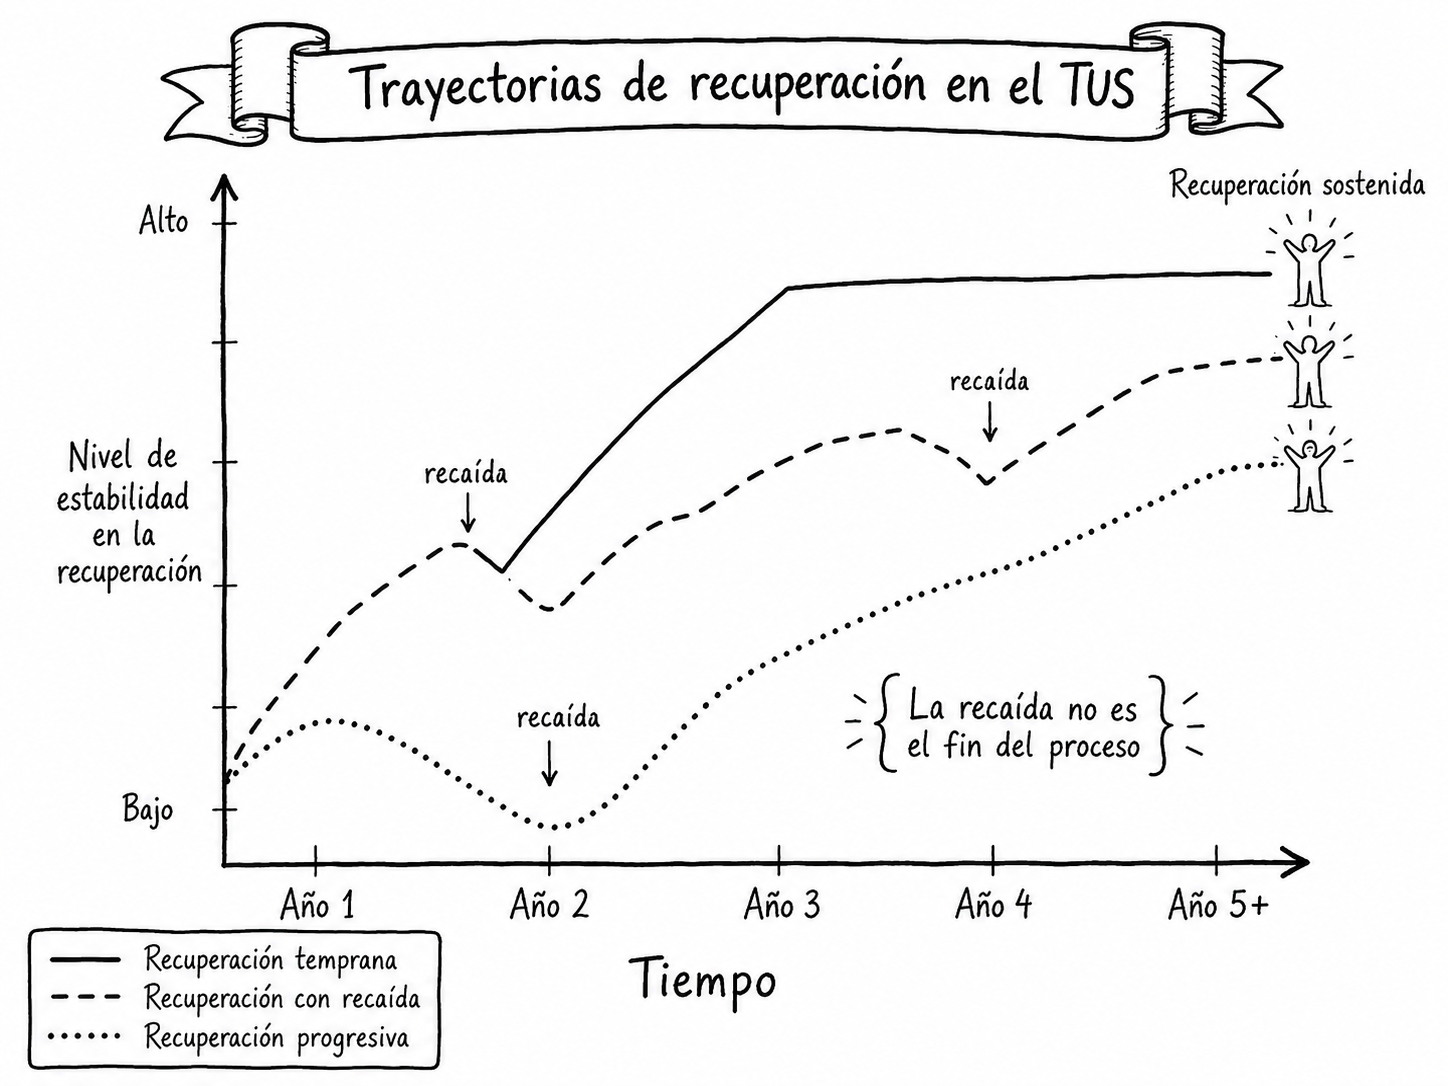
\includegraphics[width=0.8\textwidth]{reincidencia.png}
		\caption{Trayectorias de recuperación en el Trastorno por Uso de Sustancias (TUS). \textit{Elaboración propia basada en el modelo de cronicidad y recovery del National Institute on Drug Abuse (NIDA, 2024).}}
	\end{figure}
	
	Esta comprensión tiene consecuencias pastorales directas. El acompañante que entiende la recaída como parte del proceso no abandona a la persona en el momento de mayor vulnerabilidad —que es precisamente cuando más se necesita presencia—, sino que ajusta el acompañamiento a la nueva situación. La recaída es una \textbf{señal, no una sentencia}.
	
	\momento{Respuesta a las objeciones}
	
	\begin{enumerate}
		\def\labelenumi{\arabic{enumi}.}
		
		\item
		\submomento{A la primera objeción:} La recaída no borra lo aprendido ni anula el tiempo de recuperación previo. Las modificaciones neurobiológicas, los vínculos reconstruidos, las herramientas adquiridas y la historia de recuperación permanecen. La recaída exige un ajuste, no un reinicio desde cero.
		
		\item
		\submomento{A la segunda objeción:} Las trayectorias de \textit{recovery} documentadas muestran que la recaída ocurre también en personas con alta motivación y compromiso real con el proceso. No es un indicador de falta de voluntad, sino una expresión de la complejidad biológica, psicológica y social del TUS. Reducir el acompañamiento en ese momento es el error más costoso que puede cometer un agente pastoral o clínico.
		
		\item
		\submomento{A la tercera objeción:} No existen personas «irrecuperables». Las investigaciones a largo plazo muestran que incluso quienes atraviesan múltiples recaídas a lo largo de años alcanzan, en su mayoría, recuperación sostenida. Lo que varía es el tiempo y el tipo de acompañamiento necesario. La pastoral de la esperanza\index{esperanza!pastoral de la} no abandona a nadie en el camino.
	\end{enumerate}
	
	
	
	\subsection{Artículo 5: Alteración estructural de la neurotransmisión en el espacio intersináptico}
	
	\momento{Planteo del tema: La infiltración en el sistema de comunicación cerebral.} El cerebro humano funciona como una computadora biológica sumamente compleja donde miles de millones de células, llamadas neuronas, se organizan en circuitos y redes para controlar cada una de nuestras funciones. Sin embargo, este sistema no es impenetrable; las sustancias psicoactivas (SPA) tienen la capacidad de infiltrarse en este lenguaje químico, distorsionando los mensajes que definen quiénes somos y cómo percibimos la realidad.
	
	\momento{Pregunta central: ¿De qué manera la SPA altera la neurotransmisión y el espacio intersináptico?} Se cuestiona si el impacto de las sustancias es una simple amplificación del placer o si se trata de una alteración estructural en la forma en que las neuronas intercambian información en ese espacio microscópico de separación.
	
	\momento{Posturas u objeciones existentes}
	
	\begin{enumerate}
		\def\labelenumi{\arabic{enumi}.}
		
		\item
		\textbf{Parece que las drogas simplemente añaden sensaciones nuevas}, sin modificar el <<idioma>> o los procesos naturales con los que el cerebro ya cuenta para funcionar.
		
		\item
		\textbf{Parece que todas las sustancias actúan bajo el mismo mecanismo en la sinapsis}, sugiriendo que no hay diferencia entre cómo una sustancia deprime o estimula el sistema.
		\item
		\textbf{Parece que el mensaje químico se transmite con normalidad}, asumiendo que la droga solo aumenta el volumen de la señal, pero no su contenido.
	\end{enumerate}
	
	\momento{Fundamento o criterio de discernimiento} Sin embargo, el cerebro se comunica mediante neurotransmisores que viajan a través del \textbf{espacio intersináptico} para adherirse a receptores, funcionando como una \textbf{llave en una cerradura}. Las SPA logran su efecto precisamente porque \textbf{interfieren con la forma en que las neuronas envían, reciben y procesan estas señales}.
	
	\momento{Tesis y desarrollo argumental}\\ Respondemos que la alteración en el espacio intersináptico interrumpe la comunicación normal, ya que la señal química no puede ser cancelada ni limitada. Al verse saturados por la `inundación' o engañados por el `impostor', los receptores fuerzan al cerebro a una \textbf{neuroadaptación}: una respuesta defensiva donde la neurona reduce su número de cerraduras (receptores) para intentar protegerse del exceso de estímulo, lo que inicia el proceso de tolerancia.
	
	\momento{Respuesta a las objeciones}
	
	\begin{enumerate}
		\def\labelenumi{\arabic{enumi}.}
		
		\item
		\submomento{A la primera objeción:} La SPA no solo añade sensaciones, sino que altera el proceso de comunicación básica. Al interferir con los transportadores o imitar neurotransmisores, la sustancia \textbf{secuestra la maquinaria existente} para enviar señales distorsionadas.
		
		\item
		\submomento{A la segunda objeción:} Existen mecanismos diferenciados. Mientras unas sustancias \textbf{activan las neuronas por imitación} (como los opioides), otras las fuerzan a \textbf{liberar cantidades excesivas} de químicos naturales al impedir su limpieza en la sinapsis (como los estimulantes).
		\item
		\submomento{A la tercera objeción:} El mensaje no es el mismo. Las sustancias que imitan a los neurotransmisores naturales activan las redes de forma viciada o errática, produciendo una comunicación que el cerebro no puede regular por sí solo y que termina `rompiendo' el equilibrio de los circuitos de supervivencia
		
	\end{enumerate}
	
	\subsection{Artículo 6: La paradoja de la voluntad cautiva: el querer compulsivo sin agrado hedónico}
	
	\momento{Planteo del tema} \\
	Las crónicas territoriales recogen de manera constante el testimonio desgarrador de hermanos en situación de consumo crónico que expresan con lucidez: \textit{Ya no disfruto la sustancia, la aborrezco, pero no puedo dejar de buscarla}. Frente a la mirada social condenatoria que asume que la persona en situación de dependencia continúa consumiendo por puro deleite o persistencia hedonista, se hace necesario discernir cómo la alteración del sistema de saliencia motivacional consume la esclavitud del sujeto. El manual debe integrar este fenómeno para dotar de realismo científico y pastoral el abordaje de las fases más severas de la dependencia.
	
	\momento{Pregunta central} \\
	¿Debe la perseverancia en el consumo crónico interpretarse como una búsqueda continua de placer o como la manifestación de un trastorno del querer compulsivo disociado del goce real?
	
	\momento{Posturas u objeciones existentes} \\
	\begin{itemize}
		\item \submomento{Objeción 1:} Parece que si un individuo expone su salud, sus vínculos y su dignidad en la búsqueda de una sustancia es porque el placer físico obtenido sigue siendo superior a cualquier otro estímulo, lo que situaría el problema exclusivamente en la debilidad de la voluntad ante el deleite corporal.
		\item \submomento{Objeción 2:} Parece que sostener que una persona actúa movida por un querer compulsivo que ya no le produce agrado desdibuja su responsabilidad moral, reduciendo el pecado del consumo a un automatismo biológico ajeno al libre albedrío.
	\end{itemize}
	
	\momento{Fundamento o criterio de discernimiento} \\
	Este doloroso escenario encuentra su iluminación teológica en la descripción paulina de la contradicción interna del ser humano: \textit{No hago el bien que quiero, sino el mal que no quiero} (Rom 7, 19\label{rom7.19}). El magisterio eclesial actual retoma esta intuición al definir la adicción severa como una pérdida de la libertad originaria, donde las pasiones desordenadas y el secuestro neurobiológico anulan la intencionalidad del sujeto, dejándolo atrapado en una inercia materialista que vacía su existencia de todo propósito vital.
	
	\momento{Tesis y desarrollo argumental}\\ \\
	Respondemos que la adicción severa es fundamentalmente un trastorno del querer compulsivo (\textit{wanting}) y no del agrado hedónico (\textit{liking}), lo que representa la consumación de la esclavitud química a través de tres precisiones clínicas y pastorales:
	\begin{enumerate}
		\item \textbf{La validación del sufrimiento del hermano:} La evidencia científica contemporánea valida la verdad del testimonio territorial. Debido a los mecanismos de tolerancia orgánica, el placer que la sustancia producía en las etapas iniciales disminuye de forma drástica hasta desaparecer; sin embargo, el impulso motivacional dopaminérgico se independiza del disfrute, obligando al sujeto a ejecutar la conducta de búsqueda a pesar del sufrimiento y el dolor secundario que esta le genera.
		\item \textbf{La tiranía de la atención secuestrada:} El circuito mesolímbico descarrilado satura la atención del individuo. Aunque la razón y el corazón del hermano reconozcan la destrucción de su proyecto de vida, la saliencia de incentivo asignada mecánicamente a la sustancia opera como una fuerza ciega que nubla la corteza prefrontal\marginnote{Cfr. art.~\ref{art:cortex} (Juzgar, Las sustancias y el organismo, Definición..., Riesgos...)}, el freno biológico de los impulsos, impidiendo la deliberación consciente.
		\item \textbf{La desvitalización de las exigencias originales:} Al quedar el sistema de recompensa atrapado en este monólogo químico del querer compulsivo, la búsqueda de sentido, el proyecto de vida y la apertura a lo trascendente quedan anestesiados. El sujeto ya no decide en libertad; es la inercia del circuito dañado la que gestiona su energía vital, confirmando que la adicción no es una fiesta hedonista, sino el sepulcro de la agencia humana.
	\end{enumerate}
	
	\momento{Respuesta a las objeciones} \\
	\begin{enumerate}
		\item \submomento{A la primera:} La idea de que quien padece un TUS crónico consume por placer es una creencia infundada que la propia neurobiología desmiente y que el estigma social utiliza para justificar el descarte. La ciencia demuestra que lo que sostiene la conducta es la tiranía del circuito dopaminérgico de la anticipación hipertrofiado, coexistiendo con un vacío absoluto de deleite físico, lo que transforma la experiencia en un tormento existencial crónico.
		
		\item \submomento{A la segunda:} Reconocer la fractura de la voluntad no anula la responsabilidad, sino que fundamenta la necesidad urgente de una gracia liberadora y de una red de cuidados comunitarios. La persona conserva su dignidad ontológica intacta, pero su libertad está lisiada; por tanto, la comunidad organizada actúa como el andamiaje afectivo externo indispensable para restaurar su capacidad de decidir y devolverle el protagonismo de su historia a través de una pedagogía de la ternura.
	\end{enumerate}
	
	
	\subsection{Artículo 7: Compromiso de funciones vitales en el tronco del encéfalo, amígdala y corteza prefrontal}
	
	\momento{Planteo del tema: La arquitectura de la voluntad y la supervivencia} El cerebro humano no es una masa uniforme, sino un sistema de circuitos interconectados que regulan desde los latidos del corazón hasta las decisiones más complejas. Las sustancias psicoactivas (SPA) no impactan el sistema nervioso al azar, sino que alteran zonas específicas responsables de mantener la vida y permitir la autonomía del individuo.
	
	\momento{Pregunta central} ¿Qué funciones vitales se ven comprometidas cuando las drogas afectan el tronco del encéfalo, la amígdala o la corteza prefrontal\marginnote{Cfr. art.~\ref{art:cortex} (Juzgar, Las sustancias y el organismo, Definición..., Riesgos...)}? Se cuestiona si el impacto es una alteración pasajera o si representa una degradación de los mecanismos biológicos esenciales para la supervivencia.
	
	\momento{Posturas u objeciones existentes}
	
	\begin{enumerate}
		\def\labelenumi{\arabic{enumi}.}
		
		\item
		\textbf{Parece que el daño cerebral se limita a la memoria}, asumiendo que las funciones físicas automáticas están protegidas.
		
		\item
		\textbf{Parece que la incapacidad para dejar de consumir es una falla moral}, ignorando que el cerebro sufre cambios físicos que anulan biológicamente la capacidad de frenar impulsos.
		\item
		\textbf{Parece que las sobredosis son eventos accidentales}, sin comprender que se originan por la depresión química de los centros de control vital.
	\end{enumerate}
	
	\momento{Fundamento o criterio de discernimiento} Sin embargo, la ciencia confirma que la adicción es una enfermedad cerebral porque las sustancias cambian su estructura y funcionamiento de manera perdurable. El consumo altera zonas necesarias para la vida e impulsa un uso compulsivo que escapa al control voluntario.
	
	\momento{Tesis y desarrollo argumental}\\ Respondemos que el compromiso de estas tres áreas cerebrales pone en riesgo la integridad física y la libertad del individuo debido a la alteración de circuitos específicos:
	
	\begin{itemize}
		
		\item
		\textbf{Tronco del encéfalo (El regulador de la vida):} Controla funciones automáticas como la frecuencia cardíaca, la respiración y el sueño. Sustancias como los \textbf{opioides} afectan este sector, lo que explica por qué una sobredosis puede detener la respiración y causar la muerte.
		\item
		\textbf{Amígdala extendida (El centro del estrés):} Gestiona la ansiedad y la irritabilidad. Bajo consumo crónico, este circuito se vuelve hipersensible; cuando la droga falta, el malestar es tan profundo que la persona ya no consume por placer, sino para aliviar un estado de estrés insoportable.
		\item
		\textbf{Corteza prefrontal (El <<freno>> del cerebro):} Es\index{corteza prefrontal|textbf} la zona responsable de pensar, planificar y tomar decisiones. Al verse dañada, la persona pierde el control de sus impulsos y prioriza el consumo por encima de cualquier responsabilidad familiar o laboral.
	\end{itemize}
	
	\momento{Respuesta a las objeciones}
	
	\begin{enumerate}
		\def\labelenumi{\arabic{enumi}.}
		
		\item
		\submomento{A la primera objeción:} El compromiso del tronco del encéfalo demuestra que las drogas afectan la mecánica básica de la vida (respiración y pulso), no solo la memoria.
		
		\item
		\submomento{A la segunda objeción:} Lo que se interpreta como <<falta de voluntad>> es una alteración física en la corteza prefrontal\index{corteza prefrontal!maduración a los 25 años|textbf}. Como esta zona termina su maduración hacia los \textbf{25 años}, el individuo (especialmente el joven) carece del equipo biológico completo para evaluar riesgos.
		\item
		\submomento{A la tercera objeción:} La sobredosis es la evidencia máxima del impacto en el tronco del encéfalo, donde se <<apagan>> las funciones vitales al inundar los receptores cerebrales.
	\end{enumerate}
	
	\newpage
	
	\section[Diferencias según la etapa en el ciclo vital, sexo y contexto]{Diferencias según la etapa en el ciclo vital, por sexo y por contexto}
	
	Esta sección explora cómo la vulnerabilidad biológica y social no es un fenómeno uniforme, reconociendo que el impacto de las sustancias psicoactivas (SPA) varía profundamente según el ciclo vital, el sexo y el contexto del individuo. Se analiza la singularidad de la mujer, quien presenta una mayor sensibilidad fisiológica por el efecto \marginnote{Cfr. art.~\ref{art:telescopio} (Juzgar, Las sustancias y el Organismo, Diferencias según..., La respuesta fisionógica...)} y su distribución de tejido adiposo. Asimismo, se aborda la fragilidad crítica de las infancias y adolescencias, cuyo desarrollo neuronal ---específicamente de la corteza prefrontal--- culmina recién hacia los 25 años, así como la realidad invisibilizada del consumo tardío en adultos mayores. Finalmente, el estudio se sitúa en el contexto territorial, evaluando el impacto del narcotráfico, la situación de calle y la exclusión estructural, factores que obligan a trascender el enfoque meramente clínico hacia un acompañamiento integral, humanizado y situado en la realidad de los más descartados.
	
	
	\subsection{Artículo 1: Vulnerabilidad biológica aumentada en adolescentes y jóvenes}
	
	\momento{Planteo del tema: La inmadurez del centro de mando.} La adolescencia
	y la juventud no son solo etapas de transición social; son periodos de una
	profunda metamorfosis biológica. Durante estos años, el cerebro atraviesa un
	proceso de refinamiento estructural que determina cómo el individuo procesará
	el placer, el riesgo y el autocontrol. Cuando una SPA interfiere en este diseño
	<<en construcción>>, el impacto es más severo y duradero que en un adulto.
	
	\momento{Pregunta central: ¿Por qué los adolescentes y jóvenes son biológicamente más vulnerables al desarrollo de un trastorno por uso de sustancias (TUS)?}
	
	Se cuestiona si esta fragilidad responde a una falta de disciplina o de voluntad, o si existen razones fisiológicas específicas que explican por qué la transición hacia la dependencia es mucho más rápida en ellos.
	
	\momento{Posturas u objeciones existentes}
	
	\begin{enumerate}
		\def\labelenumi{\arabic{enumi}.}
		
		\item
		\textbf{Parece que el consumo es solo una cuestión de voluntad}, asumiendo
		que un joven tiene la misma capacidad racional que un adulto para evaluar riesgos y decir <<no>>.
		
		\item
		\textbf{Parece que un joven de 18 o 20 años ya posee madurez suficiente}
		para discernir los riesgos del consumo, puesto que legalmente ya se le
		considera adulto en la mayoría de las sociedades.
		
		\item
		\textbf{Parece que la precocidad del consumo no influye en la gravedad},
		creyendo que probar drogas a edades tempranas es solo una anécdota y no
		un factor que altere permanentemente la estructura neuronal.
		
		\item
		\textbf{Parece que el entorno social es el único culpable}, asumiendo que
		la estructura del cerebro no juega un papel relevante en la rapidez con
		la que se desarrolla una dependencia.
		
	\end{enumerate}
	
	\momento{Fundamento o criterio de discernimiento} 
	
	\marginnote{Cfr. Influencias macro en las capacidades de crianza (cap. 6)}
	
	Sin embargo, contra esto,
	la neurociencia establece que el cerebro continúa desarrollándose hasta los
	\textbf{25 años}. La \textbf{corteza prefrontal}\marginnote{Cfr. art.~\ref{art:cortex} (Juzgar, Las sustancias y el organismo, Definición..., Riesgos...)} —responsable de evaluar
	situaciones, tomar decisiones razonadas y controlar los impulsos— es la última
	zona en madurar. El consumo temprano de SPA ocurre por tanto en un órgano que
	aún no ha terminado de instalar sus mecanismos de control, lo que genera una
	brecha crítica entre la capacidad de sentir y la capacidad de decidir.
	
	\momento{Tesis y desarrollo argumental}\\
	Respondemos que la vulnerabilidad de los jóvenes se asienta en tres pilares
	neurobiológicos críticos que el acompañante pastoral debe conocer:
	
	\begin{itemize}
		
		\item
		\textbf{Inmadurez de la corteza prefrontal (el <<freno>> biológico):}
		Esta\index{corteza prefrontal!vulnerabilidad adolescente} zona es la última en madurar, completando su desarrollo alrededor de
		los 25 años. Al no estar conectada completamente con las emociones, el
		adolescente carece de un \textbf{freno biológico efectivo} que le permita
		medir consecuencias a largo plazo, quedando dominado por el impulso y la
		búsqueda de gratificación inmediata. Existe aquí una brecha crítica entre
		la ley y la biología: aunque la mayoría de edad legal se fije a los 18
		años, el centro neurológico de evaluación de riesgos no está consolidado
		hasta promediar los 25.
		
		\item
		\textbf{Alta neuroplasticidad\marginnote{Cfr. art.~\ref{art:neuroplasticidad} (Juzgar, Brevísimo Glosario)} y aprendizaje anómalo:} El cerebro joven es
		extremadamente plástico para facilitar el aprendizaje. Debido a que las SPA
		utilizan los mismos procesos de la memoria, el cerebro joven <<aprende>> a
		ser adicto con una velocidad y una fuerza que no ocurren en el cerebro
		maduro. El consumo antes de los 25 años puede dejar además
		\textbf{deficiencias permanentes} en la estructura neuronal que aún no
		había terminado de consolidarse.
		
		\item
		\textbf{Hiperreactividad del circuito de recompensa:} En un cerebro sediento
		de novedades, las ráfagas masivas de dopamina\marginnote{Cfr. art.~\ref{art:dopamina} (Juzgar, Las sustancias y el organismo, La farmacodinámica..., Art. 1...)} provocadas por las SPA —hasta
		diez veces superiores a lo natural— <<enseñan>> al organismo a priorizar la
		sustancia por encima de cualquier otro aprendizaje sano, instalando la
		dependencia con una rapidez desmedida.
		
	\end{itemize}
	
	\momento{Respuesta a las objeciones}
	
	\begin{enumerate}
		\def\labelenumi{\arabic{enumi}.}
		
		\item
		\submomento{A la primera objeción:} No es solo voluntad. La inmadurez del
		<<freno>> cerebral genera una incapacidad orgánica para la inhibición;
		el sistema físico del joven simplemente no responde al deseo de detenerse
		ante el estímulo masivo de la sustancia.
		
		\item
		\submomento{A la segunda objeción:} Existe una brecha crítica entre la ley y
		la biología. Tratar a un joven como un adulto maduro en términos biológicos
		es un error técnico: la neurociencia demuestra que el centro de evaluación
		de riesgos no está consolidado hasta los 25 años, independientemente de lo
		que establezca la legislación.
		
		\item
		\submomento{A la tercera objeción:} La precocidad es determinante. El
		aprendizaje adictivo antes de los 18 años se graba en la arquitectura
		cerebral con una fuerza desmedida, haciendo que la dependencia sea más
		severa, más duradera y potencialmente generadora de daños estructurales
		permanentes.
		
		\item
		\textbf{A la cuarta objeción:} El entorno es crucial, pero la
		\textbf{vulnerabilidad biológica potencia los riesgos ambientales}. Un
		cerebro en desarrollo expuesto a un entorno de oferta de drogas es
		incomparablemente más propenso a sufrir una neuroadaptación que un cerebro
		maduro en las mismas circunstancias.
		
	\end{enumerate}
	
	\subsection{Artículo 2: Influencia de la neuroplasticidad en la rapidez del aprendizaje adictivo}
	
	\momento{Planteo del tema: La maleabilidad biológica como factor de riesgo.} El cerebro humano no nace como una estructura rígida, sino como un órgano en constante remodelación que se adapta a las experiencias del entorno. Esta capacidad, fundamental para la supervivencia y la adquisición de conocimientos, alcanza su punto máximo durante la infancia y la adolescencia. Sin embargo, en el contexto de las sustancias psicoactivas (SPA), esta flexibilidad biológica se transforma en una vulnerabilidad crítica, permitiendo que el circuito adictivo se instale con una velocidad y profundidad que no ocurre en el cerebro adulto.
	
	\momento{Pregunta central: ¿Qué papel juega la neuroplasticidad\marginnote{Cfr. art.~\ref{art:neuroplasticidad} (Juzgar, Brevísimo Glosario)} en la rapidez con la que el cerebro joven aprende la conducta adictiva?} Se cuestiona si la rapidez con la que un joven desarrolla un trastorno por uso de sustancias (TUS) es simplemente una falta de madurez conductual o si responde a una propiedad física del cerebro que acelera el aprendizaje del hábito adictivo por encima de otros aprendizajes sanos.
	
	\momento{Posturas u objeciones existentes}
	
	\begin{enumerate}
		\def\labelenumi{\arabic{enumi}.}
		
		\item
		\textbf{Parece que el aprendizaje de un hábito negativo toma el mismo tiempo para todos}, asumiendo que la repetición de una conducta genera adicción con la misma rapidez en un adolescente que en un adulto de 40 años.
		
		\item
		\textbf{Parece que la neuroplasticidad es un proceso exclusivo para aprendizajes positivos}, como idiomas o música, y que no interviene en la formación de patologías como la adicción.
		\item
		\textbf{Parece que la adicción es solo una elección voluntaria}, ignorando que existen cambios físicos tangibles en la estructura neuronal provocados por el estímulo de la droga.
	\end{enumerate}
	
	\momento{Fundamento o criterio de discernimiento} Sin embargo, las fuentes definen la \textbf{neuroplasticidad} como la habilidad del cerebro para cambiar físicamente con base en los estímulos a los que es sometido. La ciencia de la prevención indica que el trastorno por uso de sustancias se considera un \textbf{fenómeno paralelo a los procesos del aprendizaje}, lo que significa que el cerebro <<aprende>> a ser adicto utilizando los mismos mecanismos que usa para memorizar información.
	
	\momento{Tesis y desarrollo argumental}\\ Respondemos que la \textbf{neuroplasticidad es el factor que acelera la transición hacia la dependencia} en el cerebro joven, funcionando como un acelerador biológico de la enfermedad por las siguientes razones:
	
	\begin{itemize}
		
		\item \textbf{La adicción como aprendizaje anómalo:} El cerebro aprende a ser adicto usando los mismos mecanismos que usa para memorizar información, pero a una velocidad mucho mayor. Debido a que las SPA liberan oleadas de dopamina\marginnote{Cfr. art.~\ref{art:dopamina} (Juzgar, Las sustancias y el organismo, La farmacodinámica..., Art. 1...)} mucho mayores a las naturales, el cerebro joven ---que es extremadamente plástico--- se adapta físicamente a la droga en un periodo mucho más corto que el de un adulto.
		\item
		\textbf{Persistencia del aprendizaje temprano:} Lo que el cerebro asimila antes de los 17 años mediante la formación de nuevas conexiones tiende a permanecer mucho más tiempo. Por ello, el <<aprendizaje>> de la adicción en la juventud se graba con una fuerza desmedida en la arquitectura cerebral que se está consolidando.
		\item
		\textbf{Sustitución de circuitos sanos:} La ráfaga masiva de dopamina cambia la conectividad de las neuronas, facilitando que el joven repita el consumo de forma automática. Esto desplaza el aprendizaje de habilidades sociales y emocionales necesarias para la vida adulta, secuestrando la capacidad de crecimiento del individuo.
	\end{itemize}
	
	\momento{Respuesta a las objeciones}
	
	\begin{enumerate}
		\def\labelenumi{\arabic{enumi}.}
		
		\item
		\submomento{A la primera objeción:} El cerebro adolescente está <<programado>> para cambiar intensamente ante los estímulos; por lo tanto, el periodo de exposición necesario para volverse dependiente es \textbf{mucho más corto} en comparación con un adulto.
		
		\item
		\submomento{A la segunda objeción:} La neuroplasticidad es un \textbf{mecanismo biológico neutro}. El cerebro no tiene la capacidad de distinguir si un estímulo es `bueno' (como aprender un idioma) o `malo' (como el consumo de SPA); simplemente se adapta físicamente al estímulo más potente. En este caso, la intensidad química de la droga gana la carrera frente a los estímulos naturales.
		\item
		\submomento{A la tercera objeción:} Aunque el inicio sea una decisión, la neuroplasticidad convierte esa conducta en un \textbf{cambio estructural permanente}. Como el `freno' cerebral (corteza prefrontal\marginnote{Cfr. art.~\ref{art:cortex} (Juzgar, Las sustancias y el organismo, Definición..., Riesgos...)}) aún no ha terminado de madurar hacia los \textbf{25 años}, el joven queda sin herramientas físicas para detener un hábito que su cerebro ya ha aprendido a un nivel biológico profundo
	\end{enumerate}
	
	
	\subsection{Artículo 3: La respuesta fisiológica diferenciada y el efecto según el sexo biológico}
	
	\momento{Planteo del tema} 
	Históricamente, los estudios sobre la adicción y la toxicocinética de las sustancias psicoactivas (SPA) se han centrado mayoritariamente en sujetos masculinos, lo que ha generado una profunda brecha de conocimiento sobre cómo el consumo afecta de manera distinta a las mujeres. Sin embargo, la fisiología humana no es neutra; el sexo biológico determina variables críticas e inapelables en la absorción, el metabolismo, la distribución, la permanencia y la eliminación de las sustancias en el organismo.
	
	\momento{Pregunta central} 
	¿Qué diferencias vinculadas a la condición sexual existen en la respuesta fisiológica ante las SPA y por qué el organismo femenino presenta una mayor vulnerabilidad estructural y metabólica hacia el daño sistémico y la dependencia? Se cuestiona si el impacto orgánico de las drogas es uniforme entre sexos o si responde a mecanismos anatómicos específicos que aceleran la cronicidad del trastorno en la mujer.
	
	\momento{Posturas u objeciones existentes}
	\begin{enumerate}
		\item \textbf{Parece que la respuesta a las drogas depende exclusivamente de la dosis y el peso corporal}, asumiendo que un hombre y una mujer de igual tamaño reaccionarán de la misma forma y que el impacto orgánico es uniforme si se ajustan las dimensiones físicas.
		\item \textbf{Parece que el tejido adiposo es un componente pasivo e irrelevante en la adicción}, creyendo que las drogas solo actúan mientras circulan en el torrente sanguíneo y que, una vez limpia la sangre en pocos días, el cuerpo queda completamente libre de la sustancia.
		\item \textbf{Parece que la rapidez con la que se desarrolla una dependencia o la mayor sensibilidad de la mujer es una cuestión puramente conductual o psicológica}, ignorando la existencia de factores metabólicos y anatómicos demostrados que aceleran el proceso de deterioro.
	\end{enumerate}
	
	\momento{Fundamento o criterio de discernimiento} 
	Sin embargo, la evidencia científica y la práctica clínica confirman que las variables biológicas alteran radicalmente la farmacocinética de las SPA según el sexo. La mayoría de las sustancias psicoactivas poseen una alta liposolubilidad, lo que significa que se disuelven y depositan con facilidad en los tejidos grasos. Este criterio técnico, sumado a las diferencias en la composición hídrica y metabólica, fundamenta lo que científicamente se define como el \textit{efecto telescopio\label{art:telescopio}}: la tendencia demostrada de la mujer a progresar de forma mucho más rápida que el hombre desde el uso inicial hasta el desarrollo de un Trastorno por Uso de Sustancias (TUS) y la aparición de consecuencias médicas graves.
	
	\momento{Tesis y desarrollo argumental}\\ 
	Respondemos que las diferencias sexuales en la respuesta fisiológica son profundas, persistentes y se asientan en cuatro pilares biológicos fundamentales:
	
	\begin{itemize}
		\item \textbf{Niveles de agua corporal y concentración plasmática:} Las mujeres tienen, proporcionalmente, menos agua en el cuerpo que los hombres. Al tener menos sangre y menos agua para disolver la sustancia, ante dosis iguales de SPA, esta alcanza niveles de \textbf{toxicidad más altos} en la sangre de la mujer, elevando drásticamente el riesgo de daños orgánicos prematuros como la cirrosis hepática.
		
		\item \textbf{Distribución sistémica del tejido adiposo como imán biológico:} Mientras que el varón concentra la grasa principalmente en zonas localizadas (vientre y espalda), el cuerpo de la mujer posee tejido adiposo distribuido de forma sistémica en todo su organismo. Al ser las SPA liposolubles, las moléculas de la droga son atraídas magnéticamente por este tejido, transformando la anatomía femenina en un gran reservorio biológico y dinámico3.
		
		\item \textbf{Impregnación prolongada y dificultad en la desintoxicación:} Esta acumulación generalizada en los depósitos de grasa provoca que la carga química permanezca impregnada en el organismo de la mujer durante mucho más tiempo que en el del varón. La toxicidad persiste de forma latente y no se elimina con una simple limpieza de sangre de pocos días, lo que ralentiza y complejiza significativamente el proceso natural de desintoxicación biológica.
		
		\item \textbf{El efecto telescopio y la velocidad del daño estructural:} Como consecuencia directa de la convergencia entre una mayor concentración hídrica inmediata y una retención lipídica prolongada, la transición hacia la dependencia severa y el deterioro estructural de los órganos ocurre en un periodo de tiempo notablemente menor en la mujer, consolidando una vulnerabilidad metabólica que condiciona todo el abordaje clínico.
	\end{itemize}
	
	\momento{Respuesta a las objeciones}
	\begin{enumerate}
		\item \submomento{A la primera objeción:} No basta con evaluar el peso corporal; la proporción interna de agua y grasa varía estructuralmente por sexo, lo que altera de manera radical la farmacocinética, elevando la concentración de la sustancia en el torrente sanguíneo de la mujer y acelerando la progresión hacia el daño físico.
		
		\item \submomento{A la segunda objeción:} El tejido graso no es pasivo; funciona como un \textbf{reservorio dinámico}. El fenómeno clínico del \textbf{<<viaje seco>>} demuestra que el cuerpo puede liberar de vuelta al torrente sanguíneo sustancias que quedaron acumuladas en las grasas incluso meses después del último consumo, confirmando que la aparente limpieza sanguínea inicial no equivale a una desintoxicación total.
		
		\item \submomento{A la tercera objeción:} La rapidez del deterioro o sensibilidad femenina tiene una base orgánica y anatomofisiológica demostrada a través del efecto telescopio. La velocidad en la cronicidad del trastorno no responde a factores psicológicos o conductuales aislados, sino a variables metabólicas objetivas que aceleran la destrucción de los tejidos y fijan la dependencia biológica.
	\end{enumerate}
	
	\subsection{Artículo 4: Riesgos biológicos en el embarazo}
	
	\momento{Planteo del tema: La vulnerabilidad del inicio de la vida.} El consumo de sustancias psicoactivas (SPA) durante la gestación no representa solo un riesgo para la salud materna, sino que constituye una \textbf{intrusión química} en un organismo en formación que carece de mecanismos de defensa propios. Esta problemática marca el desarrollo físico y cognitivo del niño antes de que este tenga la oportunidad de nacer en un entorno saludable.
	
	\momento{Pregunta central} ¿Qué riesgos específicos presenta el embarazo y qué consecuencias tiene para el recién nacido ante el consumo de SPA? Se cuestiona si el daño se limita al momento del parto o si genera secuelas permanentes en la estructura cerebral y la calidad de vida del infante.
	
	\momento{Posturas u objeciones existentes}
	
	\begin{enumerate}
		\def\labelenumi{\arabic{enumi}.}
		
		\item
		\textbf{Parece que la placenta actúa como un filtro infalible}, sugiriendo que el feto está protegido de las toxinas externas.
		
		\item
		\textbf{Parece que las sustancias <<legales>> (tabaco o alcohol) son menos dañinas} que las ilegales, minimizando el impacto de un consumo ocasional.
		\item
		\textbf{Parece que el síndrome de abstinencia solo afecta a los adultos}, ignorando que un bebé puede nacer con dependencia física severa.
	\end{enumerate}
	
	\momento{Fundamento o criterio de discernimiento} 
	
	\marginnote{Cfr. Abordajes diferenciados para mujeres (cap. 6) y Espiritualidad en la mujer (cap. 7)}
	
	Sin embargo, las fuentes técnicas establecen que las SPA atraviesan directamente el torrente sanguíneo hacia el feto. Al ser sustancias en su mayoría \textbf{liposolubles}, pasan fácilmente las membranas de la placenta y llegan directamente al cerebro y órganos en formación.
	
	\momento{Tesis y desarrollo argumental}\\ Respondemos que el consumo de SPA durante el embarazo genera riesgos críticos y diferenciados con consecuencias directas para el recién nacido:
	
	\begin{itemize}
		
		\item
		\textbf{Riesgos generales:} Restricción del crecimiento fetal, bajo peso al nacer y alta probabilidad de desarrollar \textbf{déficits cognitivos} y problemas de conducta a largo plazo.
		\item
		\textbf{Alcohol:} Es tóxico durante los nueve meses; el bebé puede nacer con el \textbf{trastorno del espectro alcohólico fetal (TEAF)}, que incluye anomalías faciales y disfunciones cerebrales permanentes.
		\item
		\textbf{Cocaína:} Puede provocar desprendimiento de la placenta, hemorragias graves y malformaciones cardíacas en el feto.
		\item
		\textbf{Tabaco:} Expone al feto a 7, 000 sustancias tóxicas, causando malformaciones como labio leporino y alterando permanentemente el crecimiento de los pulmones.
		\item
		\textbf{Heroína y Opioides:} Los bebés nacen con \textbf{dependencia física} y pueden morir a causa del síndrome de abstinencia si no reciben tratamiento especializado inmediato.
	\end{itemize}
	
	\momento{Respuesta a las objeciones}
	
	\begin{enumerate}
		\def\labelenumi{\arabic{enumi}.}
		
		\item
		\submomento{A la primera objeción:} La placenta no filtra las SPA; su naturaleza liposoluble les permite cruzar esta barrera con la misma facilidad con la que cruzan la barrera hematoencefálica\index{barrera hematoencefálica!y placenta} del adulto.
		
		\item
		\submomento{A la segunda objeción:} El alcohol y el tabaco son sumamente nocivos. El alcohol es tóxico durante toda la gestación y el tabaco reduce drásticamente la oxigenación fetal.
		\item
		\submomento{A la tercera objeción:} El \textbf{síndrome de abstinencia neonatal} es una realidad clínica grave; los bebés nacen con temblores y convulsiones, cuya vida corre un riesgo inminente en los primeros días tras el parto
	\end{enumerate}
	
	\subsection{Artículo 5: Consecuencias del consumo de alcohol en neonatos (SAN y TEAF)}
	
	\momento{Planteo del tema: La huella química en el inicio de la vida} El impacto de las sustancias psicoactivas (SPA) durante el embarazo debilita el desarrollo biológico del feto desde su etapa más temprana. Debido a que las SPA atraviesan la \textbf{barrera placentaria} y llegan directamente al torrente sanguíneo del feto, el bebé puede nacer con complicaciones que marcan su estructura física y su funcionamiento neurológico de por vida.
	
	\momento{Pregunta central} ¿Qué es el síndrome de abstinencia neonatal (SAN) y el trastorno del espectro alcohólico fetal (TEAF)? Se cuestiona si estos cuadros son dificultades pasajeras o si representan patologías crónicas derivadas de daños estructurales irreversibles causados por la toxicidad de las sustancias.
	
	\momento{Posturas u objeciones existentes}
	
	\begin{enumerate}
		\def\labelenumi{\arabic{enumi}.}
		
		\item
		\textbf{Parece que la abstinencia del bebé es solo una irritabilidad temporal} que desaparece a los pocos días del parto sin dejar secuelas.
		
		\item
		\textbf{Parece que solo las drogas ilegales causan estos trastornos,} asumiendo que sustancias legales como el alcohol o el tabaco tienen efectos mínimos en el recién nacido.
		\item
		\textbf{Parece que el daño por alcohol solo ocurre en el último trimestre}, sugiriendo que el consumo temprano es menos riesgoso para el desarrollo fetal.
	\end{enumerate}
	
	\momento{Fundamento o criterio de discernimiento} Sin embargo, los registros clínicos demuestran que el alcohol es tóxico durante los \textbf{nueve meses de gestación} y que sustancias como la heroína generan una dependencia física real en el bebé. El recién nacido carece de la \textbf{madurez metabólica} necesaria para procesar los residuos químicos de forma autónoma, por lo que estos cuadros requieren intervenciones especializadas inmediatas.
	
	\momento{Tesis y desarrollo argumental}\\ Respondemos que el SAN y el TEAF son las manifestaciones más graves de la exposición prenatal a sustancias, con consecuencias directas para el neonato:
	
	\begin{itemize}
		
		\item
		\textbf{Síndrome de Abstinencia Neonatal (SAN):} Es un conjunto de síntomas que ocurren cuando un bebé nace con dependencia física. Se manifiesta con una \textbf{hiperactividad autonómica}, irritabilidad extrema, temblores y problemas de sueño. A diferencia de los adultos, los recién nacidos pueden morir a causa de la abstinencia si no reciben tratamiento especializado en cuidados intensivos.
		\item
		\textbf{trastorno del espectro alcohólico fetal (TEAF):} Engloba los daños permanentes causados por la ingesta de alcohol en cualquier etapa del embarazo. Produce \textbf{discapacidad intelectual irreversible}, retrasos en el crecimiento y anomalías faciales características que limitan las expectativas de vida y la inserción social futura del niño.
	\end{itemize}
	
	\momento{Respuesta a las objeciones}
	
	\begin{enumerate}
		\def\labelenumi{\arabic{enumi}.}
		
		\item
		\submomento{A la primera objeción:} La abstinencia neonatal no es un malestar menor, sino una crisis biológica severa que puede incluir epilepsias y malformaciones cardíacas, exigiendo cuidados intensivos para estabilizar el sistema nervioso del infante.
		
		\item
		\submomento{A la segunda objeción:} El tabaco y el alcohol son sumamente dañinos. El humo del tabaco reduce el oxígeno fetal y causa malformaciones como el labio leporino, mientras que el alcohol es la causa principal de discapacidades cognitivas prevenibles.
		\item
		\submomento{A la tercera objeción:} No existe un nivel seguro de consumo de alcohol. Al ser tóxico durante todo el proceso gestacional, incluso el consumo temprano interfiere con la formación de órganos críticos y el desarrollo de la motricidad
	\end{enumerate}
	
	\subsection{Artículo 6: Mayor vulnerabilidad biológica en la pobreza y el estrés crónico}
	
	\momento{Planteo del tema: La cicatriz biológica de la exclusión} La vulnerabilidad ante las adicciones no depende únicamente de la genética o de una elección individual; está profundamente ligada al entorno. En contextos de exclusión, la biología del sujeto no permanece indemne; por el contrario, el ambiente de carencia escribe una \textbf{<<biografía química>>} en el cerebro, alterando los mecanismos naturales del placer y la recompensa mucho antes del primer contacto con una sustancia.
	
	\momento{Pregunta central} ¿De qué manera la pobreza extrema y el estrés crónico afectan biológicamente los receptores de dopamina\marginnote{Cfr. art.~\ref{art:dopamina} (Juzgar, Las sustancias y el organismo, La farmacodinámica..., Art. 1...)} (D2), aumentando la susceptibilidad a la adicción? Se cuestiona si la escasez y la tensión de la supervivencia son factores externos pasajeros o si tienen la capacidad de modificar la densidad de los neuroreceptores, creando un terreno fisiológico fértil para el trastorno.
	
	\momento{Posturas u objeciones existentes}
	
	\begin{enumerate}
		\def\labelenumi{\arabic{enumi}.}
		
		\item
		\textbf{Parece que la pobreza es solo un factor social}, sin impacto real en la arquitectura química de las neuronas.
		
		\item
		\textbf{Parece que el estrés no altera el sistema de recompensa de forma permanente}, sugiriendo que el cerebro recupera su equilibrio inmediatamente si el ambiente mejora.
		\item
		\textbf{Parece que la susceptibilidad a la adicción es igual para todos}, asumiendo que la biología del placer funciona igual en un entorno seguro que en uno de privación extrema.
	\end{enumerate}
	
	\momento{Fundamento o criterio de discernimiento} Sin embargo, desde la pastoral definimos la adicción como el síntoma de una fractura interna o un dolor profundo que el individuo intenta compensar. Existe una relación directa entre las vivencias traumáticas en hogares pobres y la alteración física de neuroreceptores específicos como el \textbf{D2}.
	
	\momento{Tesis y desarrollo argumental}\\ Respondemos que la pobreza extrema y el estrés crónico actúan como agentes disruptores de la homeostasis química del cerebro a través de los siguientes mecanismos:
	
	\begin{itemize}
		
		\item
		\textbf{Disminución de los receptores D2:} El estrés constante de la supervivencia provoca biológicamente una baja en la densidad de los receptores D2. Esto genera un \textbf{<<vacío biológico>>} donde el sistema de recompensa es incapaz de procesar el placer de estímulos naturales.
		\item
		\textbf{La droga como compensación autoterapéutica:} Ante este déficit de placer, las SPA aparecen como una forma de anestesiar la amargura y la ansiedad.
		\item
		\textbf{Activación del sistema de alerta:} El estrés crónico mantiene al individuo en un estado de hipervigilancia nerviosa, empujando al cerebro a buscar desesperadamente una vía de escape o anestesia en la droga.
	\end{itemize}
	
	\momento{Respuesta a las objeciones}
	
	\begin{enumerate}
		\def\labelenumi{\arabic{enumi}.}
		
		\item
		\submomento{A la primera objeción:} La pobreza se traduce en una alteración orgánica visible. El maltrato y la insatisfacción de las necesidades básicas influyen en la expresión de los genes y debilitan la solidez de la personalidad.
		
		\item
		\submomento{A la segunda objeción:} El estrés prolongado en la infancia afecta la maduración de la \textbf{corteza prefrontal\marginnote{Cfr. art.~\ref{art:cortex} (Juzgar, Las sustancias y el organismo, Definición..., Riesgos...)}} hasta los \textbf{25 años}, dejando deficiencias estructurales que dificultan la capacidad de decir <<no>> al impulso.
		\item
		\submomento{A la tercera objeción:} No existe igualdad biológica ante el riesgo. El \textbf{<<capital de recuperación>>} de una persona en pobreza es menor, y su sistema nervioso ya está condicionado por un entorno hostil que acelera el paso hacia la dependencia severa
	\end{enumerate}
	
	\newpage
	
	\section{Comorbilidad y Salud Integral}
	
	Esta sección, titulada \textbf{Comorbilidad y Salud Integral}, profundiza en la complejidad de los sujetos que enfrentan simultáneamente la adicción y otros padecimientos críticos, como la \textbf{patología dual\marginnote{Cfr. art.~\ref{art:dual} (Juzgar, La psiquis, Trauma...)}} y\index{comorbilidad|textbf} enfermedades infecciosas asociadas a la pobreza. Se define la patología dual como la coexistencia de un trastorno psiquiátrico de base (psicosis, neurosis o personalidad límite) con el consumo problemático, donde la sustancia suele funcionar como un \textbf{intento autoterapéutico} para anestesiar traumas profundos y una realidad vivida como insoportable. Asimismo, el manual aborda el impacto de la \textbf{tuberculosis (TBC) y el VIH}, afecciones que actúan como marcadores de vulnerabilidad y que, al no ser atendidas adecuadamente por un sistema de salud fragmentado, derivan en muertes vergonzosas y totalmente prevenibles. El eje central de esta sección es la \textbf{salud integral biopsicosocial y espiritual.}
	
	\subsection{Artículo 1: La patología dual}
	
	\momento{Planteo del tema: La intersección entre la mente y la adicción}
	El abordaje de las adicciones ha evolucionado hacia una comprensión
	clínica que reconoce la complejidad de la salud mental humana. En la
	mayoría de los casos, el consumo de sustancias no se presenta de forma
	aislada, sino que se entrelaza con padecimientos psíquicos preexistentes
	o desencadenados por el mismo uso.
	
	\momento{Pregunta central} ¿Qué es la patologíapatología dual\marginnote{Cfr. art.~\ref{art:dual} (Juzgar, La psiquis, Trauma...)} y por qué el 50\%
	de las personas con Trastorno por Uso de Sustancias (TUS) también
	presentan un trastorno mental coocurrente\index{patología dual}? Se cuestiona si la adicción
	y los trastornos mentales son eventos independientes o si existe una
	raíz común ---biológica, psicológica y social--- que explique esta alta
	coincidencia.
	
	\momento{Posturas u objeciones existentes}
	
	\begin{enumerate}
		\def\labelenumi{\arabic{enumi}.}
		
		\item
		\textbf{Parece que la adicción es el único problema real}, y que
		los síntomas mentales son efectos pasajeros de la intoxicación que
		desaparecerán al dejar la droga.
		
		\item
		\textbf{Parece que deben tratarse por separado}, en instituciones
		distintas y con especialistas que no se comuniquen entre sí.
		
		\item
		\textbf{Parece que la coincidencia es solo <<mala suerte>> genética},
		ignorando el papel de la historia de vida y los traumas del individuo.
		
	\end{enumerate}
	
	\momento{Fundamento o criterio de discernimiento} Sin embargo, desde la
	pastoral definimos la adicción no solo como una enfermedad, sino también
	como el síntoma de una \textbf{<<factura interna>>} o un dolor profundo
	que el individuo intenta compensar. Las investigaciones confirman que
	aproximadamente el \textbf{50\% de las personas con TUS} padecen al
	menos un trastorno mental, lo que obliga a un abordaje integral
	biopsicosocial y espiritual.
	
	\momento{Tesis y desarrollo argumental}\\
	Respondemos que la \textbf{patología dual} es la coexistencia de dos
	cuadros clínicos: un trastorno psiquiátrico de base (como psicosis,
	neurosis o personalidad límite) y un consumo problemático de SPA.
	Esta coocurrencia se fundamenta en los siguientes pilares:
	
	\begin{itemize}
		
		\item
		\textbf{Intento autoterapéutico:} La sustancia cumple la función de
		\textbf{anestesiar una vida intolerable}, dolorosa o amenazante
		debido a traumas previos. El consumo es una vía inmediata para
		reducir la angustia y la desregulación emocional.
		
		\item
		\textbf{Vulnerabilidades compartidas:} El consumo y los problemas
		de salud mental afectan las \textbf{mismas áreas del cerebro}, por
		lo que una predisposición psiquiátrica aumenta la propensión
		biológica a la dependencia.
		
		\item
		\textbf{Redes de memoria desadaptativas:} Vivencias traumáticas mal
		procesadas activan respuestas de lucha o fuga; la droga aparece como
		una herramienta de \textbf{<<fuga>>} ante un mundo percibido como
		hostil.
		
		\item
		\textbf{Círculo vicioso de la desconexión:} El TUS causa una
		desconexión espiritual y personal que genera un vacío interior,
		agravando el cuadro psiquiátrico inicial.
		
		\item
		\textbf{Modelos explicativos de la relación entre ambos trastornos:}
		La investigación clínica ha identificado cuatro modelos que explican
		cómo se articula la patología dual. 
		\begin{enumerate}
		\item El \textbf{modelo de factores comunes} sostiene que ambos trastornos comparten raíces genéticas, neurobiológicas y sociales ---como el inicio temprano del consumo o la condición socioeconómica desfavorable--- que predisponen al individuo a desarrollar los dos cuadros simultáneamente. 
		
		\item El \textbf{modelo del TUS secundario} plantea que un trastorno mental	primario triplica el riesgo de desarrollar una adicción, ya que la persona usa la sustancia para paliar su sufrimiento psíquico. 
		
		\item El \textbf{modelo del trastorno mental secundario} invierte la relación: es el consumo sostenido el que genera cambios neuroadaptativos que desencadenan la patología mental. 
		
		\item El \textbf{modelo	bidireccional} integra los anteriores, reconociendo que ambos trastornos se potencian mutuamente, agravando el estado del paciente y complejizando cualquier intervención.
		
		\end{enumerate}	
	\end{itemize}
	
	\momento{Respuesta a las objeciones}
	
	\begin{enumerate}
		\def\labelenumi{\arabic{enumi}.}
		
		\item
		\submomento{A la primera objeción:} El consumo problemático rara vez es
		el problema en sí mismo; es un intento de sobrellevar un cuadro de
		base descompensado. Ignorar la patología mental subyacente hace que
		el tratamiento sea ineficiente e inapropiado.
		
		\item
		\submomento{A la segunda objeción:} La fragmentación asistencial es un
		error técnico. Los pacientes duales requieren una estrategia donde
		el sistema de salud y la comunidad trabajen en red, humanizando el
		recorrido de sanación a través del acompañamiento afectuoso.
		
		\item
		\submomento{A la tercera objeción:} Aunque existen factores genéticos
		(40-60\%), la interacción con el entorno es determinante. La
		\textbf{pobreza estructural} y los vínculos de apego inseguros
		debilitan la personalidad, creando la <<grieta existencial>> donde
		se instala la patología dual.
		
	\end{enumerate}
	
	
	\subsection{Artículo 2: El impacto en el sistema inmunológico}
	
	\momento{Planteo del tema: La fragilidad orgánica y la vulnerabilidad social} El consumo de sustancias psicoactivas (SPA) no es solo un fenómeno cerebral; representa una agresión sistémica que debilita las defensas del organismo. Esta problemática sitúa al individuo en una intersección donde la salud física se ve comprometida tanto por la acción química directa como por las condiciones de marginalidad y exclusión que suelen acompañar al consumo problemático.
	
	\momento{Pregunta central} ¿Cómo afecta el consumo de SPA al sistema inmunológico y qué relación tiene con enfermedades infecciosas como el VIH, la tuberculosis y las hepatitis? Se cuestiona si la prevalencia de estas infecciones es una consecuencia biológica inevitable o si responde a una dinámica compleja donde el consumo altera la toma de decisiones y la capacidad del cuerpo para defenderse.
	
	\momento{Posturas u objeciones existentes}
	
	\begin{enumerate}
		\def\labelenumi{\arabic{enumi}.}
		
		\item
		\textbf{Parece que el VIH y la hepatitis son riesgos exclusivos de quienes se inyectan drogas}, minimizando el riesgo para otras vías de consumo.
		
		\item
		\textbf{Parece que la tuberculosis es una enfermedad vinculada solo al hacinamiento}, sin una relación intrínseca con el impacto de las sustancias.
		\item
		\textbf{Parece que la falta de medicamentos es la única causa de muerte}, asumiendo que el sistema de salud formal es suficiente por sí solo sin considerar el abandono del tratamiento.
	\end{enumerate}
	
	\momento{Fundamento o criterio de discernimiento} Sin embargo, la ciencia confirma que el consumo de SPA debilita el sistema inmunológico, volviendo a la persona significativamente más susceptible a enfermedades graves. El VIH y la tuberculosis (TBC) actúan como marcadores de vulnerabilidad que no solo están vinculados a la pobreza, sino que la perpetúan.
	
	\momento{Tesis y desarrollo argumental}\\ Respondemos que el consumo de SPA impacta la salud inmunológica a través de tres niveles críticos de vulnerabilidad:
	
	\begin{itemize}
		
		\item
		\textbf{Impacto Biológico Directo:} El uso crónico debilita la respuesta inmune, facilitando que patógenos como el bacilo de la TBC prosperen. En drogas inyectables, el riesgo es extremo: se estima que el 12, 6 \% de los usuarios viven con VIH y más de la mitad con hepatitis C.
		\item
		\textbf{Alteración de la Conducta de Riesgo:} La disminución de la inhibición y los efectos cognitivos negativos conducen a un aumento de conductas de riesgo (como relaciones sexuales sin protección), multiplicando las infecciones de transmisión sexual.
		\item
		\textbf{Barreras Sistémicas y Abandono:} El mayor peligro no es la infección en sí, sino que el trastorno por uso de sustancias (TUS) lleva a abandonar los tratamientos (TAR o esquemas para TBC). El sistema formal suele fallar al no atender la complejidad de quien vive en la calle, resultando en muertes absolutamente prevenibles.
	\end{itemize}
	
	\momento{Respuesta a las objeciones}
	
	\begin{enumerate}
		\def\labelenumi{\arabic{enumi}.}
		
		\item
		\submomento{A la primera objeción:} El riesgo de VIH en personas con TUS es \textbf{cuatro veces mayor} que en la población general, incluso sin inyección, debido a la desregulación emocional y conductual que provoca el consumo.
		
		\item
		\submomento{A la segunda objeción:} Existe una relación estrecha; el consumo genera un deterioro físico y neurológico tal que el individuo pierde la noción del autocuidado, permitiendo que la TBC progrese como coinfección junto al VIH.
		\item
		\submomento{A la tercera objeción:} El medicamento no garantiza la salud sin una \textbf{red de cuidados comunitarios}. Como veremos más adelante en el capítulo de la dimensión social, y el de las propuestas de la Parte 4 (Actuar), el acompañamiento par y los dispositivos de atención diferenciada logran éxitos terapéuticos superiores al \textbf{92 \%}, superando la rigidez del sistema hospitalario tradicional.
	\end{enumerate}
	
	\subsection{Artículo 3: Impacto del consumo de sustancias psicoactivas en la salud general}
	
	
	
	\momento{Planteo del tema: La degradación sistémica del organismo} El uso crónico de sustancias psicoactivas (SPA) no solo altera la química cerebral, sino que somete al cuerpo a una agresión constante que degrada órganos y sistemas vitales. Cuando este consumo ocurre en contextos de marginalidad y situación de calle, el daño biológico se potencia exponencialmente: la falta de vivienda, la desnutrición y la ausencia de redes de cuidado transforman enfermedades tratables en condiciones mortales.
	
	\momento{Pregunta central} ¿Cuáles son las consecuencias colaterales en la salud física (bucal, gástrica, respiratoria) derivadas de la marginalidad y el uso crónico de sustancias? Se cuestiona si estos daños son efectos secundarios menores o si constituyen una patología sistémica que requiere un abordaje integral, dado que la exclusión fragmenta la capacidad del sujeto para cuidar su propia vida.\\
	
	\momento{Posturas u objeciones existentes}
	
	\begin{enumerate}
		\def\labelenumi{\arabic{enumi}.}
		
		\item
		\textbf{Parece que el daño físico es causado únicamente por la toxicidad de la droga}, ignorando que factores como el frío, la falta de higiene y el hambre son determinantes en la aparición de estas enfermedades.
		
		\item
		\textbf{Parece que los problemas bucales o gástricos son superficiales}, asumiendo que el único foco de atención debe ser el sistema nervioso central y la desintoxicación neurológica.
		\item
		\textbf{Parece que el sistema de salud tradicional es suficiente para tratarlos}, sin considerar que la burocracia y el estigma actúan como barreras que impiden completar los tratamientos.
	\end{enumerate}
	
	\momento{Fundamento o criterio de discernimiento} Sin embargo, los datos territoriales indican que la marginalidad y el consumo crónico generan \textbf{<<gastos catastróficos>>} en salud y reducen drásticamente la expectativa de vida. La falta de una vivienda estable agudiza problemas que van desde enfermedades cutáneas hasta crisis respiratorias y gástricas graves.
	
	\momento{Tesis y desarrollo argumental}\\ Respondemos que las consecuencias físicas en estas poblaciones son profundas y se manifiestan en tres áreas críticas que el acompañante debe monitorear:
	
	\begin{itemize}
		
		\item
		\textbf{Salud Bucal y Dental:} El impacto químico de las SPA y el descuido extremo provocan llagas, enfermedades de las encías y caries severas. Durante la abstinencia, los dolores dentales se exacerban, convirtiéndose en un disparador del consumo para <<anestesiar>> el dolor.
		\item
		\textbf{Salud Gástrica y Metabólica:} La mala nutrición y el uso crónico derivan en úlceras gastrointestinales y enfermedades del hígado. El sistema digestivo pierde la capacidad de absorber nutrientes esenciales, lo que retrasa cualquier intento de recuperación neurológica.
		\item
		\textbf{Salud Respiratoria y TBC:} El consumo fumado (crack, pasta base) causa daño directo en el tejido pulmonar. La vulnerabilidad inmunológica facilita la proliferación de la \textbf{tuberculosis (TBC)}, que suele presentarse como coinfección junto al VIH en contextos de calle.
	\end{itemize}
	
	\momento{Respuesta a las objeciones}
	
	\begin{enumerate}
		\def\labelenumi{\arabic{enumi}.}
		
		\item
		\submomento{A la primera objeción:} La sustancia inicia el daño, pero la situación de calle impide que el cuerpo se recupere. Factores como la intemperie hacen que una infección respiratoria común se convierta en una neumonía fatal en personas con bajas defensas.
		
		\item
		\submomento{A la segunda objeción:} Estos problemas no son menores; la mala salud bucal y gástrica impide la nutrición adecuada, lo que hace imposible la reparación de los circuitos cerebrales dañados. Son signos visibles de una enfermedad que afecta a todo el ser.
		\item
		\submomento{A la tercera objeción:} El sistema formal tiene un <<tope>> porque solo medica, pero no ofrece la red de cuidados necesaria para asegurar que alguien en la calle complete un tratamiento. Solo el \textbf{acompañamiento comunitario} puede <<hilvanar>> estas respuestas fragmentadas para salvar la vida del sujeto.
	\end{enumerate}
	
	\subsection{Artículo 4: Adicciones comportamentales (Juego, tecnología y pornografía)}
	
	\momento{Planteo del tema: La expansión del concepto de adicción.} Históricamente, el concepto de adicción se limitaba al consumo de sustancias químicas externas. Sin embargo, la ciencia moderna y la práctica pastoral han revelado que el cerebro humano puede desarrollar vínculos adictivos con ciertas conductas ---como el juego, la pornografía o el uso excesivo de tecnologías--- de una manera asombrosamente similar a las drogas tradicionales. Esta realidad obliga a mirar más allá de la sustancia y comprender la vulnerabilidad de nuestra propia arquitectura cerebral ante estímulos de diseño digital o conductual.
	
	\momento{Pregunta central} ¿Por qué las adicciones comportamentales activan los mismos circuitos neurobiológicos que las sustancias químicas? Se cuestiona si es posible hablar de una <<enfermedad>> cuando no existe la ingesta de un químico externo o si el cerebro es capaz de generar su propia <<droga interna>> ante estímulos específicos, replicando el ciclo de dependencia.\\
	
	\momento{Posturas u objeciones existentes}
	
	\begin{enumerate}
		\def\labelenumi{\arabic{enumi}.}
		
		\item
		\textbf{Parece que estas conductas son simples pasatiempos o falta de disciplina}, ya que no existe un químico que atraviese la barrera hematoencefálica para alterar las neuronas.
		
		\item
		\textbf{Parece que no se puede hablar de adicción real si no hay un síndrome de abstinencia físico}, como el que ocurre con el alcohol o la heroína.
		\item
		\textbf{Parece que la <<adicción a la tecnología>> es un término exagerado}, puesto que estas herramientas son fundamentales para la vida moderna y no pueden compararse con el daño de las drogas.
	\end{enumerate}
	
	\momento{Fundamento o criterio de discernimiento} 
	
	Sin embargo, el cerebro humano está <<cableado>> para repetir actividades placenteras mediante el sistema de recompensa. Manuales especializados como el DSM-5\label{ds5b} ya clasifican el juego patológico dentro de los trastornos adictivos, reconociendo que las conductas pueden generar deterioros clínicos y funcionales idénticos a los de las sustancias.
	
	\momento{Tesis y desarrollo argumental}\\ Respondemos que las adicciones comportamentales activan los mismos circuitos porque secuestran la maquinaria natural del placer y el aprendizaje del cerebro:
	
	\begin{itemize}
		
		\item
		\textbf{Activación del Circuito de Recompensa:} Al igual que las drogas, conductas como las apuestas online o los videojuegos generan una hiperactividad en los ganglios basales. Aunque no haya una sustancia externa, estas actividades alteran los centros de placer mediante estímulos psicológicos intensos que disparan la dopamina\marginnote{Cfr. art.~\ref{art:dopamina} (Juzgar, Las sustancias y el organismo, La farmacodinámica..., Art. 1...)} interna.
		\item
		\textbf{De la Impulsividad a la Compulsividad:} Estas conductas suelen iniciar por búsqueda de placer, pero con el tiempo se vuelven compulsivas, impulsadas por la necesidad de evitar emociones negativas como el estrés o la ansiedad, lo cual es idéntico al ciclo de la adicción química.
		\item
		\textbf{Falla en el <<Freno>> Cerebral:} El uso persistente de estas tecnologías o juegos debilita la capacidad de la corteza prefrontal\marginnote{Cfr. art.~\ref{art:cortex} (Juzgar, Las sustancias y el organismo, Definición..., Riesgos...)} para controlar los impulsos. Esto explica por qué la persona pierde la autonomía y no puede detener la conducta a pesar de las consecuencias negativas en su vida.
	\end{itemize}
	
	\momento{Respuesta a las objeciones}
	
	\begin{enumerate}
		\def\labelenumi{\arabic{enumi}.}
		
		\item
		\submomento{A la primera objeción:} Aunque no ingrese un químico externo, el estímulo visual o interactivo dispara una cascada de neurotransmisores naturales que alteran la comunicación neuronal de forma tan potente como una droga.
		
		\item
		\submomento{A la segunda objeción:} La experiencia clínica muestra que existe un \textbf{síndrome de abstinencia conductual} caracterizado por irritabilidad, ansiedad y pensamientos obsesivos cuando se interrumpe el acceso al juego o al dispositivo.
		\item
		\submomento{A la tercera objeción:} No se trata de la herramienta, sino del uso. El diseño de muchas plataformas digitales busca expresamente <<enganchar>> al usuario, aprovechando la \textbf{neuroplasticidad\marginnote{Cfr. art.~\ref{art:neuroplasticidad} (Juzgar, Brevísimo Glosario)}} del cerebro ---especialmente el de los jóvenes--- para instalar circuitos de dependencia rápidos y severos.
	\end{enumerate}
	
	\chapter{Caminos de Integración}
	
	\begin{figure}[h!]
		\centering
		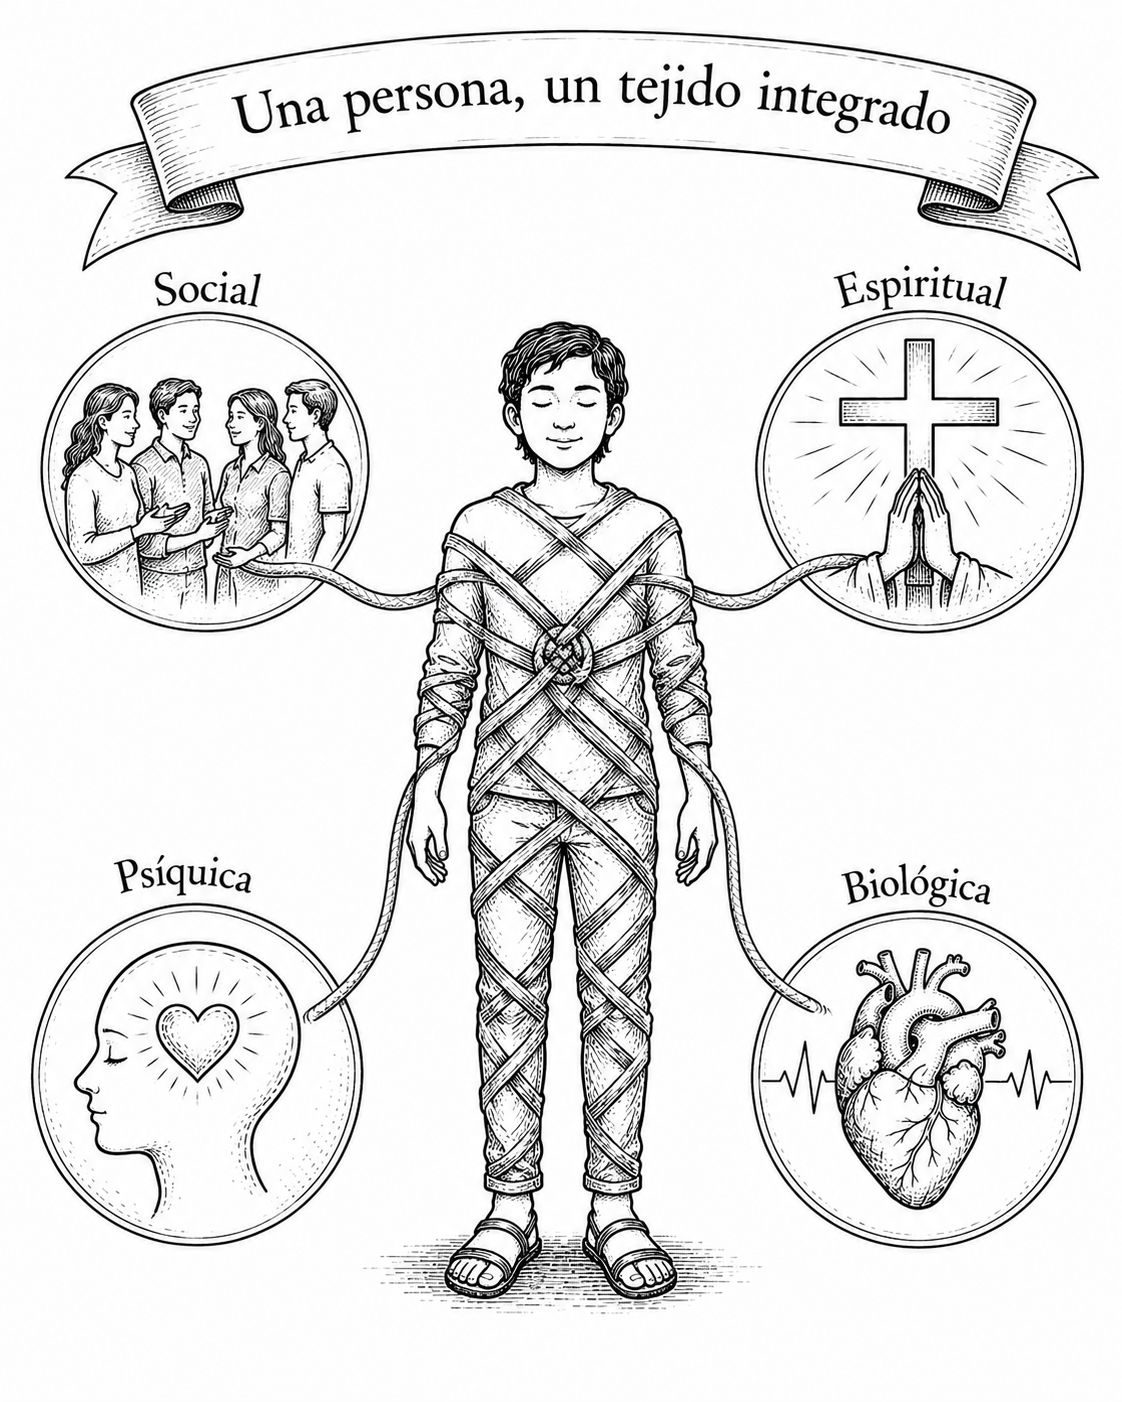
\includegraphics[scale=0.2]{tejido4dim.png}
		\caption{Las cuatro dimensiones del tejido integral}
	\end{figure}
	
	% ══════════════════════════════════════════════════════════
	% APERTURA DEL CAPÍTULO — va después de \chapter{Caminos de Integración}
	% y antes de \section{Fundamentos antropológicos}
	% ══════════════════════════════════════════════════════════
	
	A lo largo de los capítulos anteriores, ofrecimos elementos para el discernimiento\index{discernimiento} desplegados en cuatro grandes dimensiones: el ser social, el espíritu humano, la psiquis y las sustancias y el organismo. Cada dimensión iluminó un aspecto esencial de la persona que padece un trastorno por uso de sustancias, y cada una generó sus propias preguntas, sus propias tensiones y sus propios criterios de respuesta. Pero la persona no es la suma de sus dimensiones. Es una unidad viva, y el sufrimiento de la adicción la atraviesa entera.
	
	Este capítulo no agrega una dimensión más al mapa: lo recorre en su totalidad para mostrar cómo se conectan. Su función es integradora. Las tablas que siguen cruzan los temas fundamentales del acompañamiento con cada una de las cuatro dimensiones, permitiendo que el agente pastoral pueda ubicarse con precisión cuando enfrenta una situación concreta: qué está mirando, desde qué ángulo lo está mirando, y qué otras miradas podrían enriquecer su respuesta. Los artículos que las acompañan ofrecen criterios de discernimiento para las tensiones que ninguna tabla puede resolver por sí sola.
	
	Este capítulo es también el umbral entre el Juzgar y el Actuar. Quien ha recorrido este discernimiento no sale con un protocolo, sino con una mirada. Y esa mirada es la que hace posible que el Actuar tenga sentido.
	
	Una de las tensiones más importantes que recorre los capítulos anteriores merece ser nombrada antes de avanzar. El capítulo dedicado a la psiquis sostiene que el trastorno por uso de sustancias no es una estructura de personalidad cerrada sino un fenómeno que se agrega a la identidad singular del sujeto; su dignidad y su potencia de cambio son anteriores y superiores al trastorno. El capítulo dedicado a las sustancias y el organismo reconoce que el consumo crónico produce modificaciones neurobiológicas persistentes que condicionan la conducta y dificultan la recuperación. ¿Cómo puede algo «agregarse» a la identidad sin definirla si al mismo tiempo altera de manera duradera la biología del sujeto? La respuesta reside en la antropología que vertebra este manual: la persona es una unidad indivisible de cuerpo, alma y espíritu, pero esa unidad no es una equivalencia. Lo que ocurre en el cuerpo es real y no puede ignorarse, pero la persona no se reduce a su cuerpo. La adicción modifica el cerebro — eso es un hecho biológico —, pero la persona que habita ese cerebro conserva una identidad, una dignidad y una vocación que trascienden la modificación orgánica. Del mismo modo que una cicatriz se agrega al cuerpo sin convertirse en el cuerpo, el trastorno se agrega a la biografía sin convertirse en la identidad. La cicatriz es real, duele, condiciona, pero no define quién es el que la lleva. Y la misma neuroplasticidad\marginnote{Cfr. art.~\ref{art:neuroplasticidad} (Juzgar, Brevísimo Glosario)} que permitió al cerebro aprender la adicción es la que permite trazar nuevos caminos: no porque el daño se borre como si nunca hubiera existido, sino porque el cerebro humano está diseñado para seguir aprendiendo mientras viva. Esa es la base biológica de la esperanza que este manual propone.
	
	\renewcommand{\arraystretch}{1.4}
	\setlength{\extrarowheight}{3pt}
	
	\newcommand{\fuente}[1]{{\par\footnotesize\textit{(§#1)}}}
	
	\newcommand{\integracabecera}{%
		\hline
		\multicolumn{1}{|c|}{\textbf{Tema}} & 
		\multicolumn{1}{c|}{\makecell{\textbf{La dimensión}\\\textbf{social}}} & 
		\multicolumn{1}{c|}{\makecell{\textbf{El espíritu}\\\textbf{humano}}} & 
		\multicolumn{1}{c|}{\textbf{La psiquis}} & 
		\multicolumn{1}{c|}{\makecell{\textbf{Las sustancias}\\\textbf{y el organismo}}} \\ \hline
	}
	
	% ══════════════════════════════════════════════════════════
	\section{Fundamentos antropológicos}
	% ══════════════════════════════════════════════════════════
	
	{\small \begin{longtable}{|>{\RaggedRight\arraybackslash}p{0.13\linewidth}|p{0.17\linewidth}|p{0.17\linewidth}|p{0.17\linewidth}|p{0.17\linewidth}|}
		\integracabecera\endfirsthead
		\integracabecera\endhead
		\hline\multicolumn{5}{r|}{\small\textit{Continúa\ldots}}\\\endfoot
		\hline\endlastfoot
		\textbf{Dignidad Humana}
		& Derechos humanos; el derecho a ser llamado por el propio nombre frente al estigma. \fuente{6.1.2}
		& Dignidad ontológica inalienable por ser imagen de Dios; superior a cualquier pecado. \fuente{7.1.3}
		& Autoeficacia y reconocimiento de la persona como sujeto y no como objeto de asistencia. \fuente{8.1.1}
		& Deterioro físico y cognitivo que compromete la salud general pero no el valor del ser. \fuente{9.5.3} \\ \hline
		\textbf{Libertad}
		& La calle como falsa libertad; la libertad real exige condiciones mínimas de justicia social. \fuente{6.6.1}
		& Potencialidad inalienable; la adicción es una «esclavitud química» que oscurece pero no borra la libertad original. \fuente{7.2.4}
		& Recuperación de la autonomía y capacidad de decidir frente a la impulsividad del consumo. \fuente{8.4.3}
		& Secuestro del sistema de recompensa; la corteza prefrontal (freno biológico) se ve dañada. \fuente{9.3.6} \\ \hline
		\textbf{Identidad}
		& Economía popular y solidaria como motores de identidad y dignidad laboral. \fuente{6.6.4}
		& Esencia del ser; marca sagrada inalienable. \fuente{7.1.1}
		& Persona Primero: el trastorno no es la identidad, es una condición agregada. \fuente{8.1.1}
		& neuroplasticidad\marginnote{Cfr. art.~\ref{art:neuroplasticidad} (Juzgar, Brevísimo Glosario)} que permite «re-programar» la identidad hacia la salud. \fuente{9.4.3} \\ \hline
		\textbf{Tras\-cen\-den\-cia}
		& Caridad social: el afecto familiar que se abre al servicio del pueblo. \fuente{6.7.1}
		& Capacidad radical de ir más allá de sí mismo hacia Dios y el prójimo. \fuente{7.3.1}
		& Sentido de vida que permite tolerar el malestar sin evasión química. \fuente{8.4.4}
		& El cerebro que sana no se cierra sobre sí mismo: la neuroplasticidad lo abre hacia nuevos vínculos. \fuente{9.4.3} \\ \hline
		\textbf{Sentido de la Vida}
		& Pertenencia a un pueblo; protagonismo social como antídoto al descarte. \fuente{6.3.2}
		& Propósito vital como fuerza motora de la identidad. \fuente{7.1.2}
		& Logoterapia: descubrimiento de valores frente al cansancio de existir. \fuente{8.4.4}
		& Homeostasis: equilibrio químico que permite al sujeto estar en paz. \fuente{9.3.3} \\ \hline
		\textbf{Vacío Existencial}
		& Invisibilidad social y falta de horizontes en los «Ni-Ni» (jóvenes que no estudian ni trabajan). \fuente{6.2.6}
		& Patología del espíritu nacida de la falta de valores y propósito vital. \fuente{7.3.4}
		& La droga como sutura fallida para una vida percibida como insoportable. \fuente{8.4.6}
		& Disminución de receptores D2 en contextos de estrés crónico, creando un «vacío biológico». \fuente{9.3.6} \\ \hline
	\end{longtable}}
	
	% ══════════════════════════════════════════════════════════
	\section{Base biológica}
	% ══════════════════════════════════════════════════════════
	
	{\small \begin{longtable}{|>{\RaggedRight\arraybackslash}p{0.13\linewidth}|p{0.17\linewidth}|p{0.17\linewidth}|p{0.17\linewidth}|p{0.17\linewidth}|}
		\integracabecera\endfirsthead
		\integracabecera\endhead
		\hline\multicolumn{5}{r|}{\small\textit{Continúa\ldots}}\\\endfoot
		\hline\endlastfoot
		\textbf{Sustancia Psicoactiva}
		& Contextos culturales que ritualizan o profanan el uso de sustancias. \fuente{8.1.7}
		& Intento de llenar una sed de infinito con respuestas materiales. \fuente{7.3.2}
		& Modificación de la percepción, el humor y el comportamiento. \fuente{8.1.6}
		& Componente químico que atraviesa la barrera hematoencefálica y altera el SNC. \fuente{9.1.1} \\ \hline
		\textbf{Sustancias Legales}
		& El consumo de alcohol y tabaco está profundamente ritualizado en contextos sociales y familiares. \fuente{6.1.7}
		& Normalización del alcohol y el tabaco como «evangelio del bienestar». \fuente{7.3.5}
		& La distinción legal/ilegal no determina el nivel de daño; importa la relación del sujeto. \fuente{8.1.6}
		& El alcohol y el tabaco actúan sobre el SNC con los mismos mecanismos de dependencia. \fuente{9.1.4} \\ \hline
		\textbf{Sistema de Recompensa}
		& Territorio digital (videojuegos, apuestas) que activa los mismos circuitos que las drogas. \fuente{6.1.4}
		& Consumismo que satura el deseo de plenitud con placeres inmediatos. \fuente{7.3.5}
		& De la impulsividad a la compulsividad; adaptación por insensibilidad. \fuente{8.3.1}
		& Ganglios basales hiperactivados; ráfagas masivas de dopamina\marginnote{Cfr. art.~\ref{art:dopamina} (Juzgar, Las sustancias y el organismo, La farmacodinámica..., Art. 1...)}. \fuente{9.3.6} \\ \hline
		\textbf{corteza prefrontal\marginnote{Cfr. art.~\ref{art:cortex} (Juzgar, Las sustancias y el organismo, Definición..., Riesgos...)}}
		& Captación de la infancia (soldaditos) aprovechando la inmadurez biológica de los menores. \fuente{4.5}
		& Capacidad de discernimiento espiritual para elegir el bien frente al mal. \fuente{7.2.4}
		& Funciones ejecutivas: planificar, evaluar riesgos y controlar impulsos. \fuente{8.1.2}
		& Maduración tardía hasta los 25 años; es el freno biológico de las decisiones. \fuente{9.4.2} \\ \hline
		\textbf{Neu\-ro\-plas\-ti\-ci\-dad}
		& Vínculos sanos que actúan como nuevos estímulos para el cerebro plástico. \fuente{6.2.1}
		& Posibilidad de «resurrección» biológica; el cerebro puede aprender a sanar. \fuente{7.4.3}
		& Desaprendizaje de conductas nocivas; creación de nuevas redes adaptativas. \fuente{8.4.2}
		& Cada encuentro genuino deja una huella física: es la biología de la esperanza. \fuente{9.4.3} \\ \hline
	\end{longtable}}
	
	% ══════════════════════════════════════════════════════════
	\section{Dinámicas psicológicas}
	% ══════════════════════════════════════════════════════════
	
	{\small \begin{longtable}{|>{\RaggedRight\arraybackslash}p{0.13\linewidth}|p{0.17\linewidth}|p{0.17\linewidth}|p{0.17\linewidth}|p{0.17\linewidth}|}
		\integracabecera\endfirsthead
		\integracabecera\endhead
		\hline\multicolumn{5}{r|}{\small\textit{Continúa\ldots}}\\\endfoot
		\hline\endlastfoot
		\textbf{Trauma}
		& Exclusión social y pobreza estructural como escenarios de trauma complejo y desprotección. \fuente{6.6.1}
		& Trauma como velo que oculta la imagen de Dios y genera orfandad espiritual. \fuente{7.2.2}
		& El consumo funciona como intento autoterapéutico para anestesiar el dolor. \fuente{8.2.3}
		& Redes de memoria desadaptativas que desregulan el sistema autónomo (cortisol). \fuente{9.5.1} \\ \hline
		\textbf{Memoria}
		& Memoria comunitaria del barrio como herramienta de empoderamiento. \fuente{6.5.4}
		& Memoria terapéutica: reconocer las raíces para proyectar el futuro. \fuente{7.4.1}
		& Reprocesamiento de vivencias traumáticas; hilvanar la historia rota. \fuente{8.2.3}
		& Redes de memoria desadaptativas almacenadas en el sistema límbico. \fuente{9.2.8} \\ \hline
		\textbf{Emociones}
		& Emociones gestadas en el vínculo con el otro; relacionalidad trinitaria. \fuente{8.1.5}
		& Corazón como centro unificador de razón y sentimiento; búsqueda de plenitud. \fuente{7.2.3}
		& Regulación emocional; uso de diario de emociones para la introspección. \fuente{8.7.3}
		& Gatilladas por amígdala y circuitos de estrés ante redes de memoria negativas. \fuente{9.3.7} \\ \hline
		\textbf{Miedo y Ansiedad}
		& Terror impuesto por el narcotráfico; fronteras invisibles en el barrio. \fuente{4.13}
		& Desolación existencial que nubla la visión de un futuro con esperanza. \fuente{7.3.3}
		& Trauma: percepción del mundo como una amenaza constante. \fuente{8.2.3}
		& Hipersensibilidad de la amígdala ante la falta de sustancia. \fuente{9.3.7} \\ \hline
		\textbf{Salud Mental}
		& Sistema de salud fragmentado que expulsa a los pacientes complejos. \fuente{4.8}
		& Fractura de la trascendencia; orfandad emocional profunda. \fuente{7.3.1}
		& Coexistencia de TUS con trastornos psiquiátricos (psicosis, neurosis, límite). \fuente{8.2.2}
		& Desregulación del sistema nervioso central; vulnerabilidad genética. \fuente{9.5.1} \\ \hline
		\textbf{Dis\-cer\-ni\-mien\-to}
		& Acción política: discernir qué estructuras dañan el bien común. \fuente{6.7.1}
		& Sabiduría espiritual para distinguir falsas soluciones del mercado. \fuente{7.7.5}
		& Proceso de cambio: pasar de la ambivalencia a la decisión intencional. \fuente{8.3.3}
		& Recuperación de la parte racional (corteza prefrontal) para evaluar riesgos. \fuente{9.3.7} \\ \hline
	\end{longtable}}
	
	% ══════════════════════════════════════════════════════════
	\section{Vínculos y comunidad}
	% ══════════════════════════════════════════════════════════
	
	{\small \begin{longtable}{|>{\RaggedRight\arraybackslash}p{0.13\linewidth}|p{0.17\linewidth}|p{0.17\linewidth}|p{0.17\linewidth}|p{0.17\linewidth}|}
		\integracabecera\endfirsthead
		\integracabecera\endhead
		\hline\multicolumn{5}{r|}{\small\textit{Continúa\ldots}}\\\endfoot
		\hline\endlastfoot
		\textbf{Vínculos Primarios}
		& La familia como escuela de fraternidad y antídoto al individualismo. \fuente{6.2.2}
		& Mediación humana necesaria para reconocerse amado por Dios. \fuente{7.2.1}
		& Reparación de redes de memoria desadaptativas causadas por negligencia. \fuente{8.2.3}
		& Apego seguro que regula biológicamente los niveles de cortisol. \fuente{9.4.9} \\ \hline
		\textbf{Familia}
		& Escuela de fraternidad; soporte ante las influencias macroeconómicas. \fuente{6.2.2}
		& Iglesia doméstica; primer lugar de transmisión de valores y sentido. \fuente{7.2.1}
		& Enfoque sistémico: la familia se organiza en torno al síntoma. \fuente{8.4.5}
		& Factores biológicos hereditarios de vulnerabilidad. \fuente{9.4.1} \\ \hline
		\textbf{Entorno Comunitario}
		& Barrio como familia comunitaria; crianza comunitaria frente al individualismo. \fuente{6.2.4}
		& Imposibilidad de vivencia espiritual aislada; mística del encuentro. \fuente{7.9.2}
		& Capital de recuperación familiar; el rol de las familias de acogida. \fuente{8.5.3}
		& Estrés crónico ambiental que condiciona la expresión de los genes. \fuente{9.4.9} \\ \hline
		\textbf{Cultura del Encuentro}
		& Antídoto contra el individualismo; reocupación de espacios democráticos. \fuente{6.1.1}
		& Espontaneidad de la reconexión en el encuentro con los hermanos. \fuente{7.4.1}
		& Vínculo de apego seguro en centros barriales y parroquias. \fuente{8.5.3}
		& Reducción del estrés biológico mediante la hospitalidad afectiva. \fuente{9.4.9} \\ \hline
		\textbf{A\-com\-pa\-ña\-mien\-to}
		& Acompañamiento inespecífico en el territorio (calle, cárcel, hospital). \fuente{6.7.3}
		& Camino de Emaús\label{lc24.13c}; acompañar sin juzgar para restaurar la esperanza. \fuente{7.5.1}
		& Escucha activa, empatía y validación emocional. \fuente{8.7.1}
		& Abordaje técnico-profesional necesario para estabilizar la bioquímica dañada. \fuente{9.5.3} \\ \hline
		\textbf{Escucha Activa}
		& Hospitalidad de la escucha frente a la frialdad de los sistemas burocráticos. \fuente{6.1.1}
		& Valor de la palabra y el testimonio en la generación de confianza filial. \fuente{7.5.4}
		& Técnicas de parafraseo y reflejo para que el sujeto simbolice su dolor. \fuente{8.7.1}
		& Regulación del sistema nervioso a través de la presencia segura del otro. \fuente{9.3.7} \\ \hline
		\textbf{Saber Profesional vs.\ Territorial}
		& El agente pastoral territorializado posee un capital de conocimiento que se invisibiliza. \fuente{6.5.5}
		& El conocimiento espiritual del acompañante del barrio tiene autoridad propia. \fuente{7.5.4}
		& Tensión entre el modelo clínico y el saber comunitario; gestión de paridad. \fuente{8.5.4}
		& El saber técnico-clínico es necesario para comprender los procesos bioquímicos. \fuente{9.5.3} \\ \hline
	\end{longtable}}
	
	% ══════════════════════════════════════════════════════════
	\section{Estructuras sociales}
	% ══════════════════════════════════════════════════════════
	
	{\small \begin{longtable}{|>{\RaggedRight\arraybackslash}p{0.13\linewidth}|p{0.17\linewidth}|p{0.17\linewidth}|p{0.17\linewidth}|p{0.17\linewidth}|}
		\integracabecera\endfirsthead
		\integracabecera\endhead
		\hline\multicolumn{5}{r|}{\small\textit{Continúa\ldots}}\\\endfoot
		\hline\endlastfoot
		\textbf{Pobreza}
		& Exclusión estructural; falta de tierra, techo y trabajo (las 3~T). \fuente{6.3.2}
		& Desolación espiritual por falta de pertenencia y raíces en un «pueblo». \fuente{7.3.4}
		& Estrés crónico que disminuye receptores de dopamina, facilitando la adicción. \fuente{9.4.9}
		& Desnutrición y debilitamiento del sistema inmunológico ante SPA tóxicas. \fuente{9.4.9} \\ \hline
		\textbf{Justicia Social}
		& Denuncia de estructuras de pecado (nar\-co\-trá\-fi\-co) que esclavizan al pueblo. \fuente{6.7.1}
		& Caridad política: defensa de los derechos de los más rotos. \fuente{7.9.5}
		& Superación de la invisibilidad social que genera vacío existencial. \fuente{8.1.3}
		& Acceso equitativo a salud neonatal para prevenir discapacidades. \fuente{9.4.7} \\ \hline
		\textbf{Nar\-co\-trá\-fi\-co}
		& Narcopolítica y corrupción ins\-ti\-tu\-cio\-nal; el narco como organizador barrial. \fuente{4.13}
		& Cultura de la muerte; mercaderes de muerte que lucran con el dolor. \fuente{5.8.1}
		& Terror y miedo que fragmentan la subjetividad y el territorio. \fuente{8.2.1}
		& Producción de NSP y fentanilo; adulteración tóxica de sustancias tradicionales. \fuente{9.1.3} \\ \hline
		\textbf{Estigma}
		& Etiquetamiento social que expulsa al joven del sistema educativo. \fuente{6.2.6}
		& Descalificación moral que hace al sujeto sentirse indigno de Dios. \fuente{7.1.3}
		& Identidad internalizada de «adicto» que sabotea la autoeficacia. \fuente{8.1.3}
		& Segregación sanitaria en hospitales que impide el tratamiento médico. \fuente{9.5.3} \\ \hline
		\textbf{Territorio Digital}
		& Nuevo escenario de riesgo; ciudadanía digital y desconexión familiar. \fuente{6.1.4}
		& Desconexión espiritual por virtualización y soledad profunda. \fuente{7.3.5}
		& FOMO; ansiedad por la aprobación externa constante. \fuente{8.6.3}
		& Ludopatía online; alteración de circuitos de placer por notificaciones. \fuente{9.5.4} \\ \hline
		\textbf{Movilidad Humana}
		& La interculturalidad exige que la pastoral adapte sus lenguajes y metodologías. \fuente{6.6.5}
		& El desarraigo del migrante genera una orfandad espiritual. \fuente{7.3.4}
		& Los duelos migratorios no resueltos constituyen un factor de riesgo específico. \fuente{8.2.3}
		& Rupturas del hábitat biológico y vulnerabilidad. \fuente{9.4.9} \\ \hline
	\end{longtable}}
	
	% ══════════════════════════════════════════════════════════
	\section{Poblaciones específicas}
	% ══════════════════════════════════════════════════════════
	
	{\small \begin{longtable}{|>{\RaggedRight\arraybackslash}p{0.13\linewidth}|p{0.17\linewidth}|p{0.17\linewidth}|p{0.17\linewidth}|p{0.17\linewidth}|}
		\integracabecera\endfirsthead
		\integracabecera\endhead
		\hline\multicolumn{5}{r|}{\small\textit{Continúa\ldots}}\\\endfoot
		\hline\endlastfoot
		\textbf{Niñez}
		& Huérfanos funcionales; captación por bandas delictivas (soldaditos). \fuente{4.5}
		& Impacto de la falta de amor de hogar; semilla espiritual herida. \fuente{7.2.2}
		& Falta de figuras protectoras; aprendizaje adictivo acelerado por plasticidad. \fuente{8.6.2}
		& Edad de inicio promedio a los 9 años; cerebro vulnerable en construcción. \fuente{9.4.2} \\ \hline
		\textbf{Mujer y Consumo}
		& Feminización de la pobreza; la mujer como tejedora de cuidados en el barrio. \fuente{6.6.2}
		& Restauración de la imagen de Dios tras traumas de género. \fuente{7.8.3}
		& Doble condena y culpa materna; barreras específicas de acceso a tratamiento. \fuente{8.6.1}
		& Efecto \marginnote{Cfr. art.~\ref{art:telescopio} (Juzgar, Las sustancias y el Organismo, Diferencias según..., La respuesta fisionógica...)}; mayor tejido adiposo y metabolismo diferenciado. \fuente{9.4.4} \\ \hline
		\textbf{Ma\-ter\-ni\-dad}
		& Protección de la familia frente a la amenaza de pérdida de custodia. \fuente{6.6.3}
		& Madrazas comunitarias; mística de la hospitalidad maternal. \fuente{7.8.4}
		& Reparación del vínculo materno tras el trauma y el consumo. \fuente{8.6.1}
		& Riesgos biológicos en el embarazo; síndrome de abstinencia neonatal. \fuente{9.4.7} \\ \hline
		\textbf{Población Travesti-Trans}
		& Exclusión sistémica; prostitución vinculada al consumo por supervivencia. \fuente{4.11}
		& Esencia fragilizada; refugio en creencias alternativas por rechazo religioso. \fuente{7.1.3}
		& Conflictos de identidad y brecha entre imagen mental y realidad física. \fuente{8.6.1}
		& Daño físico acelerado por condiciones extremas de calle y violencia. \fuente{4.10} \\ \hline
		\textbf{Cárceles}
		& Extensión de la vulnerabilidad del barrio; la droga como moneda de cambio. \fuente{4.12}
		& El «abismo de la libertad» tras el egreso; necesidad de redención. \fuente{7.4.4}
		& Miedo al diagnóstico psiquiátrico por temor a penas más largas. \fuente{8.2.2}
		& Hacinamiento y mala salud física que agrava los trastornos neurológicos. \fuente{9.5.3} \\ \hline
	\end{longtable}}
	
	% ══════════════════════════════════════════════════════════
	\section{Respuestas pastorales y espirituales}
	% ══════════════════════════════════════════════════════════
	
	{\small \begin{longtable}{|>{\RaggedRight\arraybackslash}p{0.13\linewidth}|p{0.17\linewidth}|p{0.17\linewidth}|p{0.17\linewidth}|p{0.17\linewidth}|}
		\integracabecera\endfirsthead
		\integracabecera\endhead
		\hline\multicolumn{5}{r|}{\small\textit{Continúa\ldots}}\\\endfoot
		\hline\endlastfoot
		\textbf{Mi\-se\-ri\-cor\-dia}
		& Caridad política: incidencia en estructuras de justicia. \fuente{6.7.1}
		& Sacramentos como remedio para los heridos. \fuente{7.6.1}
		& Aceptación incondicional que permite sanar la autoestima. \fuente{8.7.1}
		& Hospital de campaña\marginnote{\textit{Amoris Laetitia} N°291\label{FALj}}: atención física urgente antes de preguntar. \fuente{9.5.3} \\ \hline
		\textbf{Mesa Compartida}
		& El centro barrial como hogar de familias que comen juntas. \fuente{6.5.1}
		& Eucaristía: alimento para los débiles; signo de fraternidad. \fuente{7.6.2}
		& Sana la fractura interna del descarte al sentirse invitado y valioso. \fuente{8.5.1}
		& Recuperación de la nutrición física básica en comunidad. \fuente{9.5.2} \\ \hline
		\textbf{Llamar por Nombre}
		& Vínculo frente a la deshumanización administrativa. \fuente{6.1.2}
		& Reconocimiento de la dignidad ontológica única e irrepetible. \fuente{7.1.3}
		& Salida del anonimato; superación de la identidad de «adicto». \fuente{8.1.3}
		& Reconocimiento del sujeto biológico singular, no estandarizado. \fuente{9.3.3} \\ \hline
		\textbf{Fe Encarnada}
		& Una Iglesia que sale al encuentro del excluido en el territorio. \fuente{6.7.3}
		& La espiritualidad se mide por su encarnación en vínculos concretos. \fuente{7.5.6}
		& Coherencia entre valores y acciones como factor de salud psíquica. \fuente{8.7.2}
		& La fe verificada en el servicio regula el estrés del acompañante. \fuente{9.4.9} \\ \hline
	\end{longtable}}
	
	% ══════════════════════════════════════════════════════════
	\section{La ética del cuidado como criterio transversal}
	% ══════════════════════════════════════════════════════════
	
	\subsection{Artículo 1: ¿Abstencionismo o Reducción de daños?}
	
	\marginnote{Lc 10, 33-34\label{lc10.33} — \textit{Pero un samaritano que iba de camino llegó adonde estaba, y, al verlo, se conmovió. Acercándose, vendó sus heridas, echándoles aceite y vino}}
	
	\momento{Planteo del tema} En la práctica pastoral\index{ética del cuidado|textbf} concreta, los agentes que acompañan a personas con trastornos por uso de sustancias suelen encontrarse ante una disyuntiva que se percibe como inevitable: optar por el modelo abstencionista —que orienta todo el proceso hacia la supresión total del consumo como condición de recuperación— o por el enfoque de reducción de daños —que prioriza la disminución de los riesgos asociados al consumo sin exigir la abstinencia como requisito de acceso al acompañamiento—. Esta tensión, lejos de ser meramente técnica, tiene consecuencias pastorales profundas, pues define quién es acompañado y en qué condiciones. El desafío consiste en discernir si esta tensión constituye una verdadera contradicción que obliga a elegir, o si existe un criterio superior capaz de integrarla sin disolver ninguno de los dos polos.
	
	\begin{figure}[h!]
		\centering
		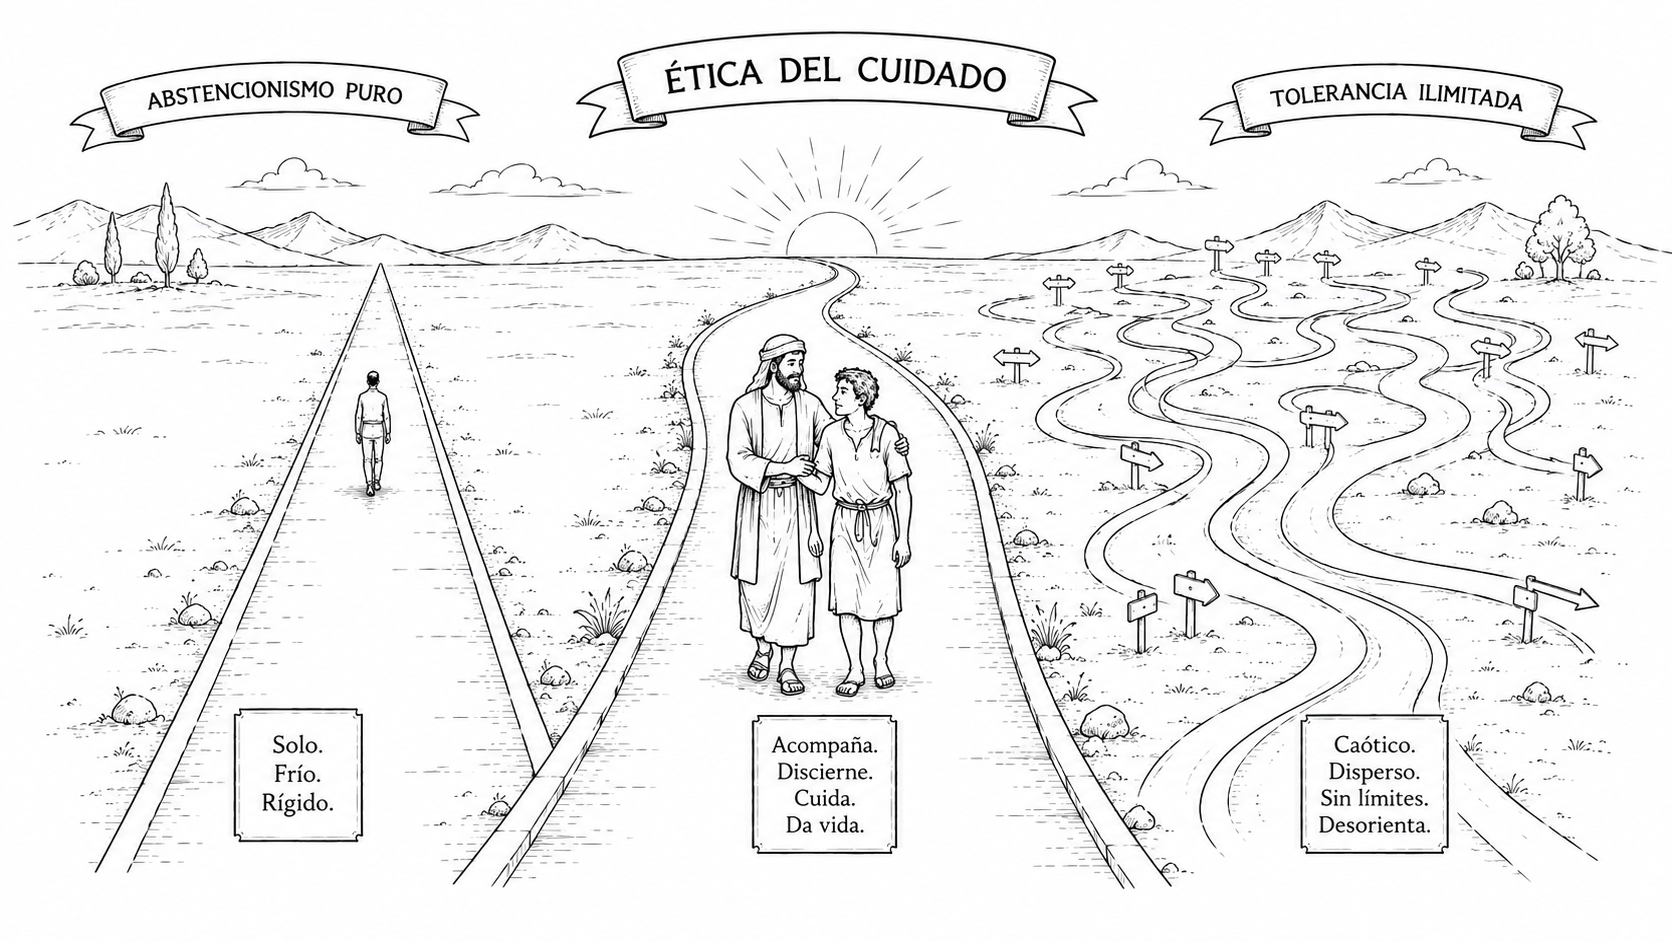
\includegraphics[scale=0.2]{cuidado.png}
		\caption{La ética del cuidado entre el abstencionismo y la reducción de daños}
	\end{figure}
	
	
	\momento{Pregunta central} ¿Deben los agentes pastorales elegir entre el modelo abstencionista y el enfoque de reducción de daños, o existe un criterio de discernimiento capaz de orientar la acción sin forzar esa elección?
	
	\momento{Posturas u objeciones existentes}
	
	\begin{itemize}
		\item \submomento{Objeción 1:} Parece que el enfoque de reducción de riesgos y daños implica un abandono de la persona, puesto que al no orientar el proceso hacia la abstinencia total renuncia a la aspiración de su recuperación plena. Aceptar el consumo como dato permanente sería conformarse con menos de lo que el hermano merece, privándolo de la posibilidad de alcanzar su máxima dignidad y autonomía.
		
		\item \submomento{Objeción 2:} Parece que el modelo abstencionista abandona igualmente a la persona, puesto que al condicionar el acompañamiento al logro de la abstinencia, termina soltando a quien no la alcanza. El que recae, el que no puede o no quiere dejar de consumir, queda sin red. La exigencia del resultado se convierte, en los hechos, en una forma de exclusión encubierta.
		
		\item \submomento{Objeción 3:} Parece que ambas lógicas son incompatibles entre sí, y que la pastoral no puede sostenerse en la ambigüedad. Mantener los dos enfoques simultáneamente generaría confusión en los equipos, incoherencia en los dispositivos y desconfianza en quienes son acompañados. Sería necesario, por lo tanto, optar por uno u otro paradigma con claridad institucional.
	\end{itemize}
	
	\momento{Fundamento o criterio de discernimiento} El error de fondo en las tres objeciones es el mismo: suponer que el criterio primero del acompañamiento pastoral es el resultado clínico —la abstinencia lograda o el daño reducido— cuando en realidad el criterio primero es la dignidad\index{dignidad} de la persona. La \textbf{ética del cuidado}\index{ética del cuidado|textbf} no es un punto medio entre dos modelos técnicos, sino un paradigma de otro orden: afirma que el acceso al acompañamiento no puede estar condicionado por ningún resultado previo, sino únicamente por la condición de ser humano herido que necesita ser acompañado.
	
	Este criterio no es una novedad pastoral, sino la traducción operativa de lo que este manual ha propuesto desde el principio: la imagen del Retablo de Isenheim, donde los enfermos del monasterio de San Antonio no eran recibidos una vez sanos ni una vez dispuestos a sanar, sino en la crudeza de su llaga abierta. La Iglesia como \textit{hospital de campaña}\index{hospital de campaña|textbf}, en la expresión del Papa Francisco, no pide méritos para abrir la puerta; cura primero, y acompaña el proceso sin anticipar su desenlace. Dice Francisco: \textit{la comunidad evangelizadora se mete con obras y gestos en la vida cotidiana de los demás, achica distancias, se abaja hasta la humillación si es necesario, y asume la vida humana, tocando la carne sufriente de Cristo en el pueblo}\marginnote{Evangelii Gaudium N° 24\label{FEGe}}.
	
	Desde este criterio, la abstinencia es un \textbf{horizonte deseable y legítimo}, no una condición de inclusión. Y la reducción de daños es una \textbf{herramienta válida en determinados tramos del proceso}, no una capitulación ante el fenómeno. Ambos enfoques son instrumentos al servicio del cuidado, y el discernimiento pastoral consiste en saber cuándo y cómo desplegar cada uno, sin absolutizar ninguno.
	
	La ética del cuidado es transversal\index{ética del cuidado!transversalidad} porque no pertenece a ninguna dimensión exclusiva del abordaje —no es solo social, ni solo clínica, ni solo espiritual— sino que opera como el suelo desde el que todas las respuestas se articulan. Quien cuida no elige entre aspirar a lo mejor para el otro y acompañarlo donde está: hace las dos cosas al mismo tiempo, en el orden que la situación concreta exige.
	
	\textbf{Respuestas a las objeciones:}
	
	\begin{itemize}
		\item \submomento{A la primera:} El enfoque de reducción de daños no abandona a la persona cuando está orientado por la ética del cuidado, sino que la sostiene en el tramo del proceso donde la abstinencia todavía no es posible. Abandonar sería retirarse. Reducir el daño es permanecer al lado. La aspiración a la recuperación plena no se niega; se sostiene incluso cuando el camino es más largo y tortuoso de lo esperado.
		
		\item \submomento{A la segunda:} El modelo abstencionista no abandona a la persona cuando no confunde el horizonte con el requisito. La abstinencia como meta orienta el proceso; la abstinencia como condición lo cierra. Una pastoral que suelta al hermano que recae no está siendo fiel al ideal de recuperación, sino traicionándolo: la misericordia estructurada —como se ha desarrollado en este manual— sabe que el vínculo no se rompe ante la fragilidad, sino que se fortalece precisamente ahí.
		
		\item \submomento{A la tercera:} La aparente incompatibilidad entre ambos modelos se disuelve cuando se comprende que ninguno de los dos es el paradigma, sino herramientas dentro de un paradigma mayor. No hay contradicción entre sostener la abstinencia como horizonte y acompañar a quien todavía no puede alcanzarla. La ambigüedad que debe evitarse no es la de usar distintas herramientas según el momento, sino la de no tener criterio claro sobre para qué se usan. Ese criterio es el cuidado de la persona concreta, en su historia singular, sin abandonarla en ningún tramo del camino.
	\end{itemize}
	
	% ══════════════════════════════════════════════════════════
	\subsection{Artículo 2: Sobre el acompañamiento a quien no reconoce su problema}
	% ══════════════════════════════════════════════════════════
	
	\marginnote{Lc 15, 20\label{lc15.20} — \textit{Cuando todavía estaba lejos, su padre lo vio y se conmovió profundamente; corrió a su encuentro, lo abrazó y lo besó}}
	
	\begin{figure}[h!]
		\centering
		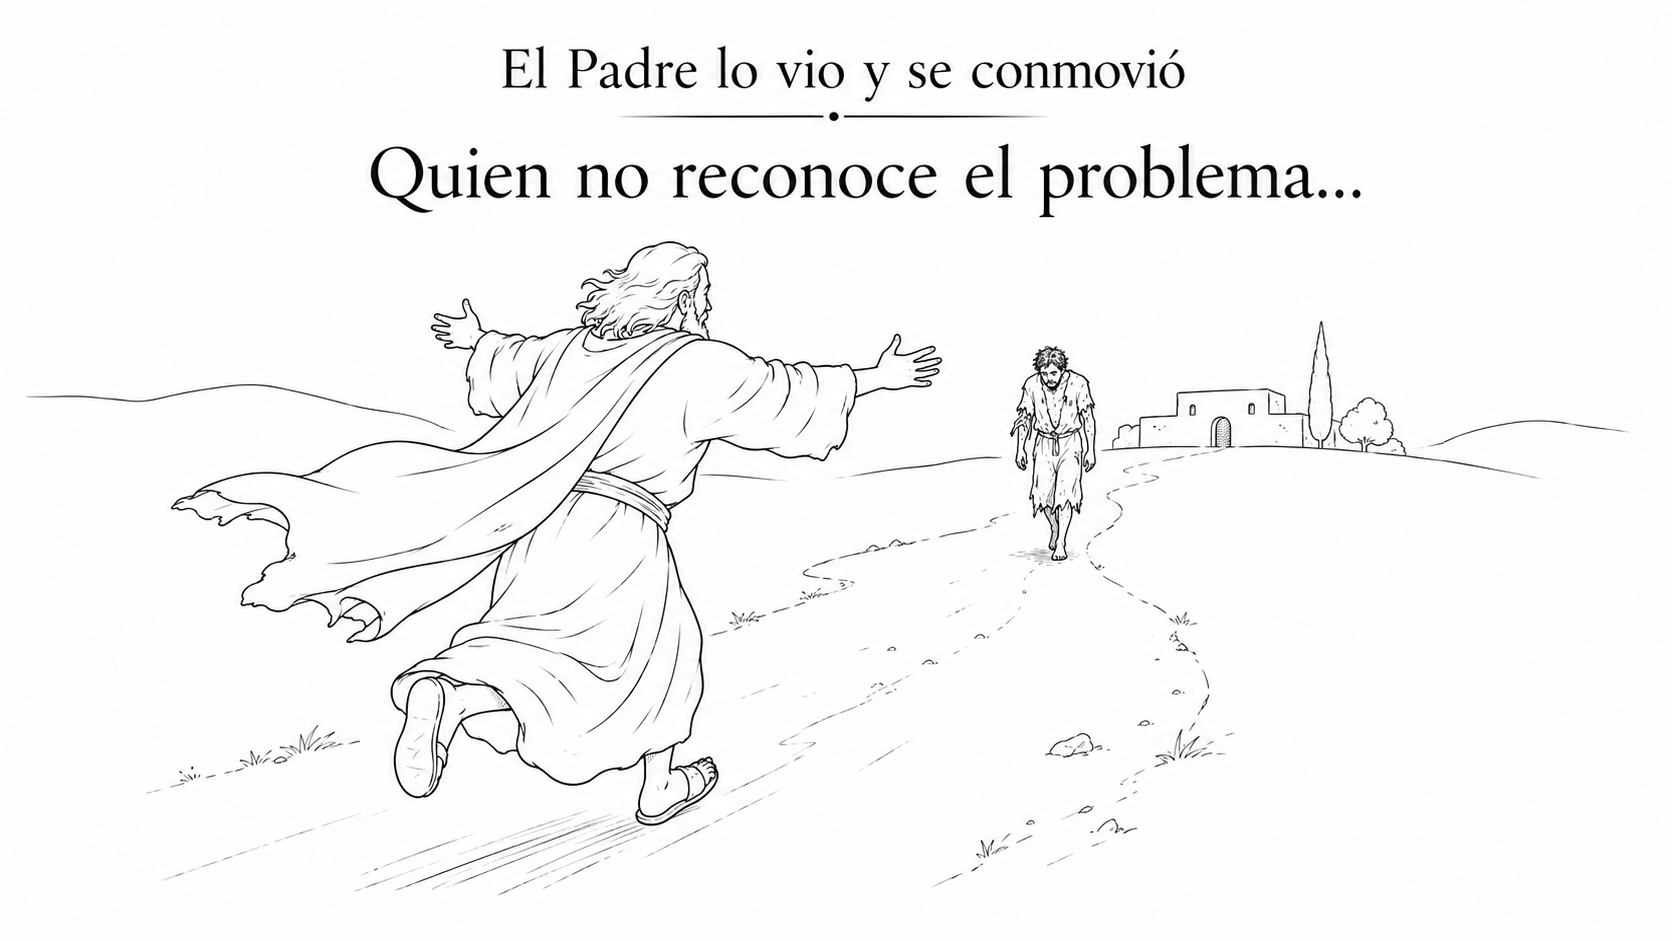
\includegraphics[scale=0.2]{padremisericordioso.png}
		\caption{El Padre misericordioso}
	\end{figure}
	
	\momento{Planteo del tema} En la práctica pastoral concreta, uno de los momentos más difíciles no es el del hermano que pide ayuda, sino el del hermano que no la pide. La persona que consume sin reconocer el daño, que rechaza el acompañamiento o que simplemente no tiene conciencia de necesitarlo, pone al agente pastoral ante una pregunta que no admite respuesta fácil: ¿tiene sentido sostener un vínculo cuando el otro no lo reconoce como tal? ¿Es legítimo acercarse a quien no ha dado señales de querer ser acompañado? ¿O debe el agente esperar a que el sujeto exprese su necesidad antes de actuar? El discernimiento pastoral requiere claridad sobre cuál es el fundamento del vínculo y en qué momento nace el deseo de cambio.
	
	\momento{Pregunta central} ¿Puede el agente pastoral sostener un acompañamiento significativo con quien no reconoce su problema ni manifiesta deseo de cambio, o debe esperar a que emerja esa motivación para iniciar el proceso?
	
	\momento{Posturas u objeciones existentes}
	
	\begin{itemize}
		\item \submomento{Objeción 1:} Parece que no se puede acompañar a quien no pide ayuda, puesto que toda intervención no solicitada viola la autonomía de la persona. Imponerse sobre alguien que no reconoce su situación como problemática sería una forma de paternalismo que desconoce su capacidad de decidir sobre su propia vida, reproduciendo la misma lógica de control que la pastoral pretende superar.
		
		\item \submomento{Objeción 2:} Parece que sostener el vínculo con alguien que consume sin reconocer el problema equivale a habilitar ese consumo. Si el agente permanece al lado sin exigir ningún cambio, podría estar enviando el mensaje implícito de que la situación es tolerable, convirtiéndose inadvertidamente en cómplice de un proceso que destruye al hermano.
		
		\item \submomento{Objeción 3:} Parece que sin motivación no hay proceso posible. El Modelo Transteórico del Cambio enseña que el sujeto en etapa de precontemplación no está listo para modificar su conducta; por lo tanto, todo esfuerzo del acompañante sería prematuro e inútil, un gasto de energía que no produce resultado y que puede terminar agotando al agente y frustrando al acompañado.
	\end{itemize}
	
	\momento{Fundamento o criterio de discernimiento} El error compartido por las tres objeciones es suponer que el vínculo\index{vínculo!como condición del cambio|textbf} viene después de la motivación, cuando en realidad ocurre exactamente al revés: \textbf{la presencia significativa\index{presencia significativa|textbf} es la condición de posibilidad del deseo de cambio}. Nadie puede desear lo que nunca ha experimentado ni siquiera como posibilidad. Y la posibilidad de una vida diferente no emerge de una decisión abstracta, sino del encuentro concreto con alguien que te ve, te llama por tu nombre y permanece al lado sin condiciones.
	
	Este principio no es una novedad pastoral: es lo que el Retablo de Isenheim lleva pintado desde el siglo XVI. Juan y la Magdalena no estaban al pie de la cruz porque el Cristo crucificado les hubiera pedido que se quedaran. Permanecieron porque su amor no necesitaba ser solicitado para sostenerse. Esa presencia que no exige reciprocidad inmediata es precisamente el modelo del acompañamiento pastoral en los momentos de mayor oscuridad.
	
	Desde la psicología del apego, la ciencia confirma lo que la fe ya sabía: la presencia regulada de otro significativo crea las condiciones neurobiológicas para que emerja el deseo. El cerebro herido por el consumo y el abandono no puede generar motivación en el vacío; necesita primero experimentar que existe alguien que no se va, que no juzga, que llama por el nombre. Ese vínculo sostenido en el tiempo actúa como andamiaje sobre el que la persona, paulatinamente, empieza a hablar, a nombrar lo que padece y a reconocer en esa presencia la primera señal de que algo mejor es posible.
	
	El agente pastoral que se acerca sin esperar que el otro pida no viola su autonomía: la \textbf{construye}. Porque la autonomía no es un dato previo que hay que respetar desde afuera, sino una capacidad que se desarrolla en el vínculo. Un sujeto arrasado subjetivamente por el consumo, el abandono y el estigma no tiene autonomía plena en el sentido abstracto del término; tiene, en cambio, la posibilidad de recuperarla si alguien permanece lo suficientemente cerca y el suficiente tiempo como para que el deseo y la autonimía tengan lugar.
	
	\textbf{Respuestas a las objeciones:}
	
	\begin{itemize}
		\item \submomento{A la primera:} La presencia significativa no impone ni interviene sobre el otro; ofrece vínculo. No hay violación de la autonomía en quedarse al lado, en llamar por el nombre, en no abandonar. La autonomía que se invoca como argumento para no acercarse es con frecuencia la indiferencia disfrazada de respeto. El agente pastoral no espera que el otro pida para acercarse, porque sabe que pedir requiere haber experimentado previamente que alguien puede responder.
		
		\item \submomento{A la segunda:} Sostener el vínculo\index{vínculo!sostener sin aprobar} no es aprobar el consumo. La presencia significativa\index{presencia significativa!y permanencia} no dice «está bien lo que hacés», sino «no te suelto aunque lo que hacés te destruya». Esa distinción es la que separa la complicidad del acompañamiento. El Retablo de Isenheim no pinta a Juan y a la Magdalena aprobando la crucifixión; los pinta resistiéndose a abandonar al crucificado. La permanencia al lado del que sufre es un acto de denuncia del sufrimiento, no de aceptación de sus causas.
		
		\item \submomento{A la tercera:} El Modelo Transteórico del Cambio no dice que el sujeto en precontemplación no puede avanzar; dice que no puede avanzar solo. La etapa de precontemplación no es un muro, es un umbral. Y los umbrales se cruzan cuando hay alguien del otro lado. La motivación no precede al vínculo: \textbf{nace de él}. El agente que permanece en ese tramo aparentemente estéril no está desperdiciando energía; está sembrando en el único suelo donde el deseo de cambio puede germinar.
	\end{itemize}
	
	
	% ══════════════════════════════════════════════════════════
	\section{Respuestas prácticas}
	% ══════════════════════════════════════════════════════════
	
	{\small \begin{longtable}{|>{\RaggedRight\arraybackslash}p{0.13\linewidth}|p{0.17\linewidth}|p{0.17\linewidth}|p{0.17\linewidth}|p{0.17\linewidth}|}
		\integracabecera\endfirsthead
		\integracabecera\endhead
		\hline\multicolumn{5}{r|}{\small\textit{Continúa\ldots}}\\\endfoot
		\hline\endlastfoot
		\textbf{Prevención}
		& Espacios promocionales (deporte/arte) para «llegar antes» que el narco. \fuente{6.5.3}
		& Educación en valores y capacidad de decir «no» a lo deshumanizante. \fuente{7.5.2}
		& Fortalecimiento de la autoeficacia y habilidades de rechazo. \fuente{8.7.2}
		& Intervención temprana para proteger el cerebro infantil. \fuente{9.4.2} \\ \hline
		\textbf{Recaída}
		& Red de apoyo para no abandonar al hermano que cae. \fuente{6.4.3} y \fuente{8.5.3}
		& La misericordia como fuerza para levantarse; no es un fracaso moral. \fuente{7.7.4}
		& Oportunidad pedagógica dentro del ciclo de cambio. \fuente{8.3.4}
		& Memoria celular y «viaje seco» por sustancias en el tejido graso. \fuente{9.2.8} \\ \hline
		
		\textbf{Lí\-mi\-te Sa\-no}
		& El límite puesto desde el vínculo, no desde el control; la norma comunitaria como abrazo protector. \fuente{6.3.3}
		& La gratuidad de Dios no es desorden; el límite expresa un amor que cuida impidiendo la autodestrucción. \fuente{6.3.3}
		& El límite sano reduce la ansiedad y entrena la voluntad mediante metas graduales y predecibles. \fuente{8.3.1}
		& La estructura predecible regula el sistema nervioso autónomo y disminuye el cortisol del estrés crónico. \fuente{9.4.9} \\ \hline
		
		\textbf{Sus\-ti\-tu\-ti\-vas}
		& Rechazo de la liberalización como solución; la abstinencia como horizonte, no como condición de acceso al cuidado. \fuente{5.9.2} y \fuente{10.8.1}
		& La libertad plena como vocación del espíritu; el acompañamiento no renuncia a ese horizonte aunque el camino sea gradual. \fuente{7.4.4}
		& La reducción de daños como herramienta válida en el tramo donde la abstinencia aún no es posible; la autonomía como meta del proceso. \fuente{8.3.2} y \fuente{10.8.1}
		& Intervención farmacológica orientada a preservar la vida y estabilizar al sujeto para que el proceso integral pueda sostenerse. \fuente{9.3.3} \\ \hline
		\textbf{Trabajo}
		& Cooperativismo frente al dinero fácil del narcotráfico. \fuente{6.3.1}
		& El trabajo como participación en la obra creadora de Dios. \fuente{7.4.4}
		& Desarrollo de habilidades vocacionales; superar el rol de asistido. \fuente{8.7.2}
		& Recuperación de ritmos circadianos y energía física por oficios. \fuente{9.5.3} \\ \hline
		\textbf{Au\-to\-cui\-da\-do}
		& Sostenibilidad de la red comunitaria; cuidado de los que cuidan. \fuente{6.7.2}
		& Teología del descanso; el derecho al ocio que glorifica a Dios. \fuente{7.7.3}
		& Manejo del burnout y la fatiga por compasión. \fuente{8.7.4}
		& Prevención del agotamiento biológico del acompañante. \fuente{9.5.3} \\ \hline
		\textbf{Gratitud}
		& Cultura del encuentro celebrada en la comunidad agradecida. \fuente{6.1.1}
		& Motor de sanación profunda; reconocimiento de milagros cotidianos. \fuente{7.7.4}
		& Reducción de la ansiedad; enfoque en las fortalezas. \fuente{8.7.3}
		& Reducción de niveles de cortisol y mejora inmunológica. \fuente{9.5.2} \\ \hline
	\end{longtable}}
	
	% ══════════════════════════════════════════════════════════
	\section{Dimensiones del proceso}
	% ══════════════════════════════════════════════════════════
	
	{\small \begin{longtable}{|>{\RaggedRight\arraybackslash}p{0.13\linewidth}|p{0.17\linewidth}|p{0.17\linewidth}|p{0.17\linewidth}|p{0.17\linewidth}|}
		\integracabecera\endfirsthead
		\integracabecera\endhead
		\hline\multicolumn{5}{r|}{\small\textit{Continúa\ldots}}\\\endfoot
		\hline\endlastfoot
		\textbf{Lógica del Tiempo}
		& Procesos artesanales frente a la lógica de franquicia institucional. \fuente{6.5.2}
		& Amistad con el tiempo; respeto por la historia sagrada del otro. \fuente{7.7.2}
		& Etapas del proceso de cambio; no se puede forzar la maduración. \fuente{8.3.1}
		& Cronómetro biológico: vida media de eliminación y procesos lentos. \fuente{9.2.10} \\ \hline
		\textbf{Inmediatez}
		& Cultura del descarte que prioriza el consumo inmediato. \fuente{5.6}
		& Falso absoluto del mercado que ofrece felicidad mágica instantánea. \fuente{7.3.5}
		& Impulsividad digital que erosiona la espera. \fuente{8.6.3}
		& Velocidad de acción: sustancias fumadas llegan al cerebro en 7 segundos. \fuente{9.2.1} \\ \hline
		\textbf{Co\-mor\-bi\-li\-dad}
		& Barreras burocráticas que impiden el acceso a salud pública. \fuente{4.7}
		& Unción de los enfermos en situaciones límite de salud física. \fuente{7.6.5}
		& Somatización del sufrimiento; abandono del tratamiento por desolación. \fuente{8.2.1}
		& Enfermedades marcadoras: TBC, VIH, daño bucal y dental. \fuente{9.5.1} \\ \hline
	\end{longtable}}
	
	% ══════════════════════════════════════════════════════════
	% CIERRE DEL CAPÍTULO — va después de la última tabla
	% y antes de \part{Actuar}
	% ══════════════════════════════════════════════════════════
	
	El discernimiento no es un ejercicio abstracto. Tiene un destino concreto: la persona que está del otro lado, con su historia singular, su llaga abierta y su deseo todavía no del todo despierto. Todo lo que se ha iluminado en esta parte del manual —la dignidad, la libertad, el vínculo, el trauma, la biología, el espíritu— converge en un solo gesto pastoral: el de quedarse al lado sin soltar.
	
	El Actuar que viene no es la aplicación mecánica de lo que se aprendió en el Juzgar. Es su verificación en la carne de la historia real. Allí, en la parroquia, en la escuela, en la cárcel, en la calle, el agente descubrirá que los criterios aprendidos necesitan ser encarnados cada vez de nuevo, en cada persona, en cada momento. Eso no es una debilidad del método: es su mayor virtud. Un manual que pudiera decirle al agente exactamente qué hacer en cada situación no lo estaría formando, lo estaría reemplazando.
	
	Lo que este manual ofrece es algo más valioso que un protocolo: una mirada capaz de ver al otro como un ser completo, roto pero no muerto, perdido pero no sin destino. Con esa mirada, ofrecemos propuestas para nuestro Actuar.
	
	
	\partsubtitle{La respuesta pastoral}
	\part{Actuar}
	\markboth{}{}
	
	\begin{center}
		\begin{minipage}{0.7\textwidth}
			\itshape
		Cuando Marcelo llegó por primera vez a la capilla, nadie sabía demasiado de él. Algunos lo habían visto deambular por el barrio desde hacía meses. Dormía donde podía: a veces en la casa de un amigo, otras en un zaguán, otras directamente en la estación. Tenía treinta y tantos años, aunque el cuerpo parecía bastante más viejo. Caminaba rápido, siempre con la cabeza baja y una campera gris aun cuando hacía calor.
		
		Entró una tarde de lluvia. En el salón parroquial estaban terminando la catequesis y preparando la merienda para los chicos. Marcelo se quedó parado cerca de la puerta, incómodo, como si estuviera listo para irse en cualquier momento. Una mujer que servía la leche con cacao lo miró y simplemente le preguntó:
		
		—¿Querés comer algo?
		
		Marcelo asintió sin hablar demasiado. Comió rápido. Después se quedó sentado solo, mirando cómo los chicos corrían de un lado al otro mientras una catequista los retaba porque estaban jugando a la pelota adentro.
		
		Nadie le preguntó enseguida qué consumía. Nadie le pidió explicaciones. Nadie le habló de tratamiento.
		
		Primero hubo una silla. Después un plato de comida. Después alguien que empezó a acordarse de su nombre.
		
		Con el tiempo empezó a aparecer cada vez más seguido. A veces ayudaba a mover mesas antes de la merienda. Otras veces desaparecía durante días enteros. Cuando volvía, traía en el cuerpo el cansancio de la calle, los ojos perdidos y el olor mezclado del humo, el vino y las noches sin dormir. Las recaídas eran constantes.
		
		Había semanas donde parecía estar mejor y de golpe volvía a perderse. Más de una vez robó cosas pequeñas para consumir. También mintió muchas veces. Algunos en la comunidad se cansaban. Otros desconfiaban. Algunos preguntaban si realmente valía la pena seguir insistiendo.
		
		Pero el párroco repetía algo sencillo: 
		
		— Las personas son más importantes que sus peores momentos.
		
		Marcelo había empezado a consumir muy joven. Primero alcohol. Después cocaína. Después bazuko o crack. Había pasado por trabajos temporarios, peleas familiares, noches en comisarías y períodos de calle. Su mamá había muerto hacía años. Con su hija casi no tenía relación. Hacía mucho tiempo que vivía sintiendo que molestaba en todos lados.
		
		Y quizás por eso lo que más le desconcertaba de la parroquia era que nadie pareciera apurado en echarlo.
		\end{minipage}
	\end{center}
	
	\begin{center}
		\begin{minipage}{0.7\textwidth}
			\itshape
			
			Un sábado, mientras preparaban la olla popular, una señora mayor le pidió ayuda para cargar unas bolsas de verduras. Marcelo la acompañó hasta la cocina y ella, sin saber demasiado de su historia, le dijo:
			
			—Gracias hijo, menos mal que llegaste porque sola no podía.
			
			Esa frase quedó resonándole durante días.
			
			“Hijo”.
			
			Hacía muchísimo tiempo que nadie lo llamaba así.
			
			La comunidad empezó lentamente a volverse parte de su vida. No de manera perfecta. No como en las historias prolijas. Hubo conflictos, cansancio, discusiones y momentos muy duros. Una noche llegó golpeado después de una pelea. Otra vez tuvieron que llevarlo al hospital porque casi no podía respirar. Más adelante apareció llorando porque un amigo del barrio había muerto consumiendo.
			
			Y la parroquia siguió ahí. A veces con palabras. A veces sin saber qué decir. A veces solamente estando.
			
			Marcelo comenzó a participar de algunas celebraciones. Al principio se quedaba atrás, cerca de la puerta. Después se animó a leer una intención en misa. Más adelante ayudaba a ordenar las sillas después de los encuentros. Un verano empezó a acompañar a los chicos en el campamento parroquial.
			
			No fue una recuperación lineal. Nunca lo son. Todavía había días malos. Todavía existía el miedo de volver a caer. Todavía convivía con heridas profundas.
			
			Pero algo había empezado a cambiar.
			
			Ya no estaba solo.
			
			Y en esa experiencia sencilla —una capilla abierta, una comunidad que conoce su nombre, una mesa compartida, alguien que lo espera cuando desaparece, alguien que vuelve a buscarlo cuando cae— Marcelo empezó lentamente a recuperar algo que creía perdido desde hacía años: la sensación de que su vida valía la pena.
			
			Tiempo después, durante una reunión, alguien le preguntó qué había sido lo más importante para él en todo ese proceso.
			
			Marcelo se quedó pensando un rato largo antes de responder.
			
			Después dijo despacio:
			
			—Yo vine porque tenía hambre… pero me terminé quedando porque acá sentí que si un día no aparecía, alguien me iba a salir a buscar.
		\end{minipage}
	\end{center}
	
	\newpage
	
	% ══════════════════════════════════════════════════════════
	% PÁRRAFO DE BISAGRA — va después de la historia de Marcelo
	% y antes de \chapter{Ámbito parroquial}
	% ══════════════════════════════════════════════════════════
	
	La historia de Marcelo no es un caso de éxito clínico. Es una historia de vínculo. Nadie le aplicó un protocolo. Nadie le diseñó un itinerario terapéutico desde el primer día. Alguien le preguntó si quería comer, y después se acordó de su nombre. Eso fue todo — y fue suficiente para que algo empezara a moverse.
	
	Las propuestas que siguen en esta parte del manual nacen de esa misma lógica. No son recetas ni modelos cerrados. Son caminos que distintas comunidades han recorrido, desde la parroquia hasta la escuela, desde el barrio hasta la cárcel, animadas por una convicción común: que el primer gesto pastoral no es técnico sino humano, y que la ética del cuidado\index{ética del cuidado} no es un principio abstracto sino una decisión concreta que se toma cada vez que alguien llega, cada vez que alguien cae, cada vez que alguien vuelve.
	
	El agente que recorre estas páginas encontrará herramientas, criterios y experiencias. Pero la pregunta que orienta todo sigue siendo la misma que se hizo aquella tarde de lluvia: \textit{¿querés comer algo?}
	
	
	
	
	\chapter{Propuestas pastorales por ámbito}
	
	
	Esta primera parte recoge orientaciones y propuestas concretas que cualquier comunidad puede poner en práctica en los distintos ámbitos donde se despliega la vida pastoral. No son modelos cerrados ni protocolos fijos. Son caminos probados que cada comunidad deberá inculturar en su propio territorio.
	
	\begin{figure}[h!]
		\centering
		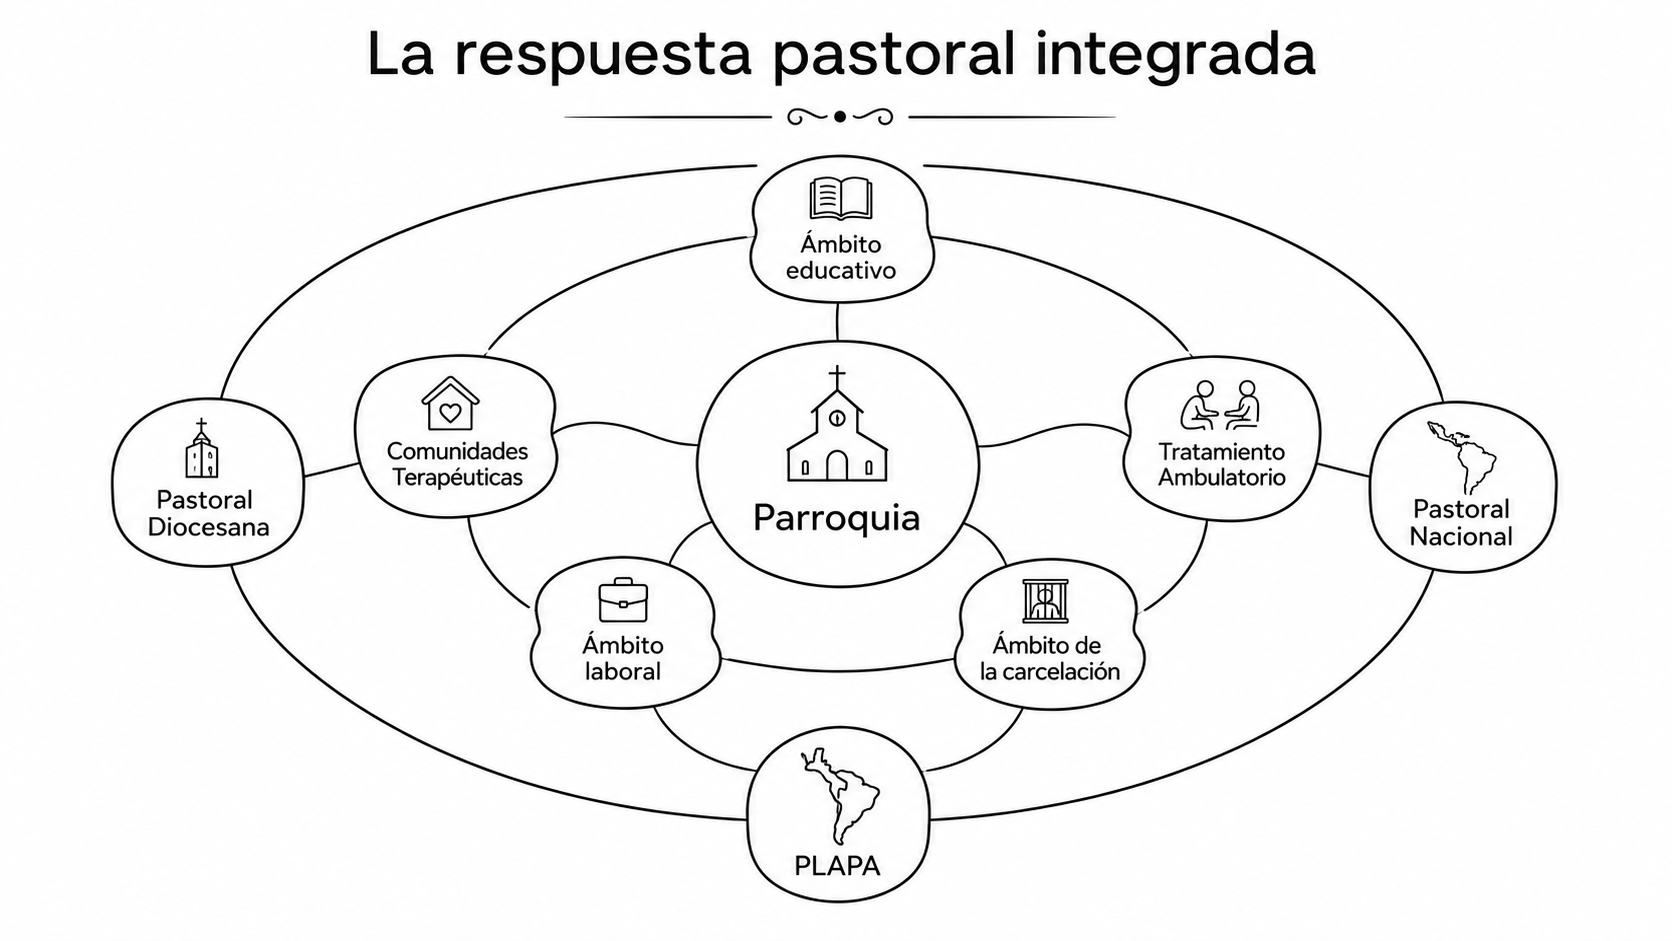
\includegraphics[scale=0.2]{anillos-de-respuesta.png}
		\caption{Los anillos de respuesta pastoral}
	\end{figure}
	
	
	\section{Ámbito parroquial}
	
	Si el diagnóstico de nuestro tiempo nos revela una crisis de vínculos y un profundo sentido de orfandad, la respuesta de la parroquia no puede limitarse solamente al culto, a la gestión de programas o a la apertura de dispositivos técnicos. La parroquia, antes que una institución que brinda servicios, está llamada a ser una comunidad que genera vida. El actuar pastoral en el mundo de las adicciones consiste, esencialmente, en ofrecer una filiación y una pertenencia allí donde el consumo ha dejado aislamiento y vacío.
	
	Esta misión se vuelve concreta cuando la parroquia logra constituirse como una verdadera casa. El primer gesto de esta transformación es la disposición de salida, que se manifiesta en la puerta de entrada y el trabajo de calle. Una comunidad que no espera a que el sufriente golpee su puerta, sino que sale a buscarlo en los márgenes, en las esquinas y en los pasillos donde la vida duele. Esta cercanía se traduce en gestos de una sencillez radical: caminar el territorio, compartir un pedazo de paz y recibir la vida como viene, sin preguntas, sin condiciones y sin juicios previos.
	
	Una vez que el vínculo se establece, la hospitalidad inicial encuentra su cauce en la creación de grupos y espacios compartidos. Partimos de la certeza de que nadie se salva solo; en un mundo que tiende a la fragmentación, la parroquia ofrece la ronda y el encuentro como ámbitos donde la palabra vuelve a tener lugar. Este proceso se sostiene mediante el acompañamiento personal, un vínculo de fidelidad y paciencia que consiste en caminar al lado de cada vida única, sosteniendo la mano en los momentos de mayor fragilidad y acompañando con paciencia los tiempos de cada proceso.
	
	La recuperación también pasa por lo cotidiano y lo simple. La vida comunitaria —compartir la mesa, organizar las tareas del día, celebrar los vínculos— devuelve a la persona el sentido de dignidad y de pertenencia a algo más grande que sus propios problemas. En este marco, los talleres y actividades de prevención (el deporte, el arte, los oficios) no son entretenimientos, sino herramientas para que cada uno pueda desplegar sus capacidades y volver a proyectar un futuro. La espiritualidad atraviesa todo este movimiento, no como una imposición, sino como una oferta de sentido que invita a descubrir a un Dios que camina en lo sencillo y que es fuente de esperanza.
	
	Entendemos que los procesos de recuperación e integración son caminos de largo aliento, marcados por avances y caídas. Por eso, el actuar parroquial implica no soltar la mano y estar dispuestos a empezar de nuevo las veces que haga falta. Este cuidado se extiende necesariamente a las familias, que sufren el desgaste del dolor y necesitan ser alojadas en su angustia. Finalmente, la parroquia reconoce que no es una isla; se sabe parte de una red comunitaria y busca articular esfuerzos con clubes, centros de salud y organizaciones del barrio, entendiendo que el territorio se cuida entre todos. Cuando la comunidad logra ser ese espacio de acogida y cuidado, se convierte en un signo de que la vida, a pesar de todo, siempre puede volver a brotar.
	
	Entendemos que hay algunas acciones que suelen ser parte de la respuesta pastoral de nuestras parroquias. Es importante que esos espacios entiendan cómo acompañar a quienes sufren por estos problemas. 
	
	\subsection{Espacios de escucha y acompañamiento espiritual:}
	Cada vida es única y necesita un vínculo cercano que la sostenga. Acompañar es caminar al lado, con paciencia y fidelidad.
	
	\textbf{Algunos gestos concretos pueden ser}: 
	\begin{itemize}
		\item Encuentros personales
		\item Visitas
		\item Estar atentos
		\item Acompañar en trámites o momentos difíciles.
	\end{itemize}
	
	\subsection{Grupos, talleres y actividades que dan vida:}
	El hacer ayuda a sanar y prevenir. Aprender, crear, moverse, descubrir capacidades abre caminos nuevos.
	
	\textbf{Algunos gestos concretos pueden ser}: 
	
	\begin{itemize}
		\item Talleres de oficio
		\item Deporte
		\item Música
		\item Arte
		\item Apoyo escolar
		\item Espacios donde cada uno pueda desplegar sus talentos
	\end{itemize}
	
	
	\subsection{Trabajo con familias:}
	Las familias también sufren y necesitan ser acompañadas. Cuidarlas es fortalecer el corazón de cada proceso.
	
	\textbf{Algunos gestos concretos pueden ser}: 
	\begin{itemize}
		\item Encuentros de padres
		\item Espacios de escucha
		\item Orientación
		\item Estar cerca en momentos de crisis
	\end{itemize}
	
	\subsection{La liturgia:}
	La liturgia es el gran momento de encuentro de las comunidades parroquiales, en el que se expresa la fe y su comprensión. Por esa razón es importante que estos problemas de nuestra gente vayan entrando en dialogo con nuestra oración comunitaria y celebración.
	
	\textbf{Algunos gestos concretos pueden ser}:
	\begin{itemize}
		\item Incorporar estos temas en la homilía
		\item Jornadas penitenciales 
		\item Adoraciones eucarísticas 
	\end{itemize}
	
	
	\subsection{Los retiros espirituales:}
	Muchas de nuestras parroquias ofrecen los llamados retiros de impacto (Cenáculo, Emaús, etc.) apoyados en testimonios de vida que generan identificación. Es importante que estos retiros tengan lugar para recibir la vida rota de la persona que consume o de sus familiares.
	
	\textbf{Algunos gestos concretos pueden ser}:
	\begin{itemize}
		\item Incorporar testimonios de personas que atravesaron estos problemas y los superaron.
		\item Planificar instancias de acompañamiento grupal para aquellas personas que luego de hacer el retiro quieren replantear su vida.
		\item Proponer a quienes hacen los retiros acciones de servicio concreto con personas en situación de calle, o exclusión social grave.
	\end{itemize}
	
	
	\subsection{El trabajo de calle:}
	La Iglesia sale al encuentro, no espera. Va a buscar, se hace cercana, se mete en la vida del barrio y abre sus puertas para que todos tengan un lugar. 
	
	\textbf{Algunos gestos concretos pueden ser}: 
	\begin{itemize}
		\item Rutas de calle 
		\item Misión en el barrio 
		\item Estar en las esquinas
		\item Abrir la parroquia con alguna comida o bebida para compartir
		\item Recibir sin preguntas ni condiciones.
	\end{itemize}
	
	\subsection{Los Centros Barriales}
	
	\subsubsection{Una puerta abierta en el barrio}
	
	El consumo problemático de sustancias no es solo un problema de salud individual: es, ante todo, un síntoma de exclusión. Detrás de cada persona que consume hay casi siempre una historia de orfandad afectiva, de derechos vulnerados, de vínculos rotos. Por eso, una respuesta que se limite a lo clínico o a lo espiritual sin enraizarse en el territorio donde esa persona vive, trabaja y sufre, llega siempre tarde y llega siempre desde afuera.
	
	La parroquia tiene una ventaja que ningún otro actor del sistema posee: ya está en el barrio. No llega al territorio; vive en él. Conoce las familias, conoce la historia, conoce los nombres. Esa inserción previa es el recurso más valioso con el que cuenta para construir una respuesta pastoral al consumo problemático, y es el fundamento sobre el que se puede montar un centro barrial.
	
	Un centro barrial no es un centro de salud, ni una comunidad terapéutica, ni un comedor. Es algo diferente y más básico: un espacio de acogida y vínculo desde el cual se articula todo lo demás. Es, para usar una imagen del lenguaje deportivo, el mediocampo: por allí pasa la pelota. Desde allí se llega a los recursos del sistema y desde allí se vuelve. Sin ese nodo territorial, las intervenciones quedan fragmentadas y las personas quedan solas en el trayecto entre un dispositivo y otro.
	
	\subsubsection{Tres ejes: cercanía, gestión y acompañamiento}
	
	La metodología del centro barrial se sostiene sobre tres ejes que no son etapas sino actitudes permanentes y simultáneas.
	
	\textbf{Cercanía.} El\index{cercanía|textbf} primer gesto no es técnico sino humano: hacer lugar. Recibir la vida como viene, sin condicionar el acceso a ningún requisito previo. La persona que llega —o a la que se va a buscar— no necesita estar lista para cambiar, ni haber tomado una decisión, ni tener resueltos sus problemas básicos. Llega como es, con sus heridas abiertas, con su historia entera. El centro barrial la recibe así, y empieza desde ahí.
	
	Esta cercanía se construye con gestos concretos: un plato de comida, un nombre recordado, una visita al domicilio, el acompañamiento a un turno médico. No son gestos auxiliares al acompañamiento: son el acompañamiento mismo en sus primeras formas. La inclusión real, no discursiva, es siempre cuerpo a cuerpo. Cada persona es sagrada; ninguna vida está de sobra.
	
	Un elemento clave de la cercanía\index{cercanía!mirada integral} es la \textbf{mirada integral}. El centro barrial no se ocupa de una parte de la persona —su consumo, su salud, su causa judicial— sino de su historia completa. Busca conocer su familia, su vivienda, sus vínculos, la red de contención con la que cuenta o que le falta. Esta mirada de conjunto es posible precisamente porque el centro está en el barrio y puede ver lo que ningún especialista externo puede ver.
	
	\textbf{Gestión.} El segundo eje es la articulación en red. El centro barrial no reemplaza al sistema de salud, a la escuela, a los organismos judiciales o a los programas estatales: los conecta con la persona. Muchas veces lo que falla no es la existencia de los recursos sino el acceso a ellos. La burocracia expulsa; los horarios excluyen; los formularios atemorizan. El centro barrial actúa como interfaz entre la persona y el sistema, acompañándola en cada trámite, cada derivación, cada internación, cada egreso.
	
	Esta función de nodo en la red es irreemplazable. Sin ella, una persona que egresa de una comunidad terapéutica queda sola. Con ella, tiene un lugar al que volver, alguien que la espera, una red que la sostiene mientras reconstruye su vida.
	
	\textbf{Acompañamiento.} El tercer eje es la continuidad del vínculo en el tiempo. Los procesos de recuperación del consumo problemático son largos, no lineales, atravesados por recaídas y retrocesos. El sistema formal de salud trabaja por episodios; el centro barrial trabaja por historias. Sostiene el vínculo antes del problema, durante el tratamiento y después del egreso. No hay un momento en que el acompañamiento termine; hay momentos en que se vuelve más o menos intenso según lo que la persona necesita.
	
	\subsubsection{Quiénes sostienen el centro}
	
	El centro barrial no requiere un equipo de profesionales para funcionar. Su fuerza está en los \textbf{voluntarios con arraigo territorial} — personas del propio barrio que conocen el territorio porque viven en él — y en los \textbf{acompañantes pares}: personas que han atravesado ellas mismas situaciones de consumo y exclusión, y que por eso tienen una credibilidad y una cercanía que ningún técnico externo puede igualar.
	
	El acompañante par no acompaña desde la teoría sino desde la experiencia del dolor, la caída y la posibilidad real de recomenzar. Su presencia dice lo que ningún discurso puede decir: que el cambio es posible porque ya ocurrió en alguien de carne y hueso, de ese barrio, con esa historia.
	
	El rol del agente pastoral o del referente eclesial es sostener la mística\index{mística} del conjunto, garantizar que el centro no pierda su identidad de acogida incondicional, y articular con las redes más amplias — parroquiales, diocesanas, institucionales.
	
	\subsubsection{El centro como espacio espiritual}
	
	El consumo problemático es, entre otras cosas, una enfermedad espiritual. No en el sentido moralista del término, sino en el más profundo: la persona que consume ha perdido con frecuencia la convicción de que su vida vale la pena vivirse. Ha perdido el sentido, la alegría, la pasión por existir.
	
	Por eso el centro barrial no es solo un dispositivo social: es un espacio donde se engendra sentido. Donde alguien te llama por tu nombre y eso ya es un acto espiritual. Donde la comunidad dice con su presencia que ninguna vida está de sobra. Donde se reaviva, de a poco y sin apuro, la pasión por vivir.
	
	La parroquia que abre un centro barrial no está ofreciendo un servicio adicional: está siendo lo que desde siempre fue llamada a ser. Un lugar donde los excluidos encuentran lugar. Una familia grande que recibe la vida como viene.
	
	\subsection{\texorpdfstring{Cómo comenzar}{Como comenzar}}
	
	No hace falta tener todo resuelto para empezar. Hace falta un espacio físico — puede ser una habitación en el salón parroquial — , un grupo pequeño de personas dispuestas a recibir, y la decisión de no juzgar a quien llegue. El resto se construye caminando.
	
	Algunos pasos concretos para el inicio:
	
	\begin{itemize}
		\item \textbf{Mapear el territorio:} ¿Quiénes son las personas en situación de consumo en el barrio? ¿Dónde están? ¿Qué recursos existen ya en la zona — centros de salud, programas municipales, organizaciones comunitarias? \marginnote{Cfr. Gn. 4, 9\label{gen49a} — \textit{¿Dónde está tu hermano?}}
		
		\item \textbf{Identificar referentes:} ¿Hay personas en la comunidad con experiencia de recuperación que podrían acompañar como pares? ¿Hay voluntarios con arraigo en el barrio dispuestos a formarse?
		
		\item \textbf{Abrir el espacio:} Un horario fijo, un lugar conocido, una puerta que siempre esté abierta. La regularidad genera confianza; la confianza genera vínculo; el vínculo genera proceso.
		
		\item \textbf{Articular con la red:} Conocer los dispositivos disponibles en el territorio — centros de salud, comunidades terapéuticas, programas de empleo, defensorías — y construir relaciones concretas con sus referentes. El centro barrial no puede hacer todo solo; su fuerza está en ser el nodo de una red que sí puede.
		
		\item \textbf{Formarse:} El acompañamiento de personas con consumo problemático requiere herramientas. La formación de los agentes no es un lujo sino una condición de sustentabilidad. Sin ella, el desgaste hace que los voluntarios abandonen y el centro se cierre.
	\end{itemize}
	
	
	
	\subsection{El abrazo a las infancias}
	
	En algunas realidades donde la edad de inicio del consumo promedia los 9 años, la parroquia no puede esperar a que el problema se manifieste en la adolescencia; debe \textit{llegar antes} a través de espacios promocionales que fortalezcan la construcción del ser social. 
	
	El actuar parroquial con las niñeces se fundamenta en el paradigma de la \textit{crianza comunitaria}\index{crianza comunitaria}. Este modelo entiende que cuando las familias son muy disfuncionales o están muy rotas, la crianza no es una tarea confinada exclusivamente a la esfera de la intimidad familiar biológica, sino que es una responsabilidad compartida por toda la comunidad. La parroquia debe constituirse como una \textit{familia grande} que ofrece amparo y pertenencia allí donde los lazos primarios se encuentran fragilizados.
	
	\subsubsection{Criterios y acciones para el trabajo parroquial}
	
	Para que este acompañamiento sea efectivo y transformador, se proponen las siguientes líneas de acción:
	
	\begin{itemize}
		\item \textbf{Priorizar lo primario:} Antes de cualquier abordaje pedagógico o espiritual profundo, la comunidad debe asegurar el derecho a la alimentación, la higiene y el abrigo. El baño, la mesa compartida y el abrazo son los primeros medicamentos que devuelven la dignidad al niño.
		\item \textbf{Espacios específicos de escucha:} Es necesario que dentro de la parroquia existan lugares donde los niños tengan su propia voz y equipos específicos que los miren. El acompañante del niño no debe ser el mismo que acompaña a la madre o al padre, para evitar sesgos y garantizar que el niño se sienta protagonista de su propio proceso.
		\item \textbf{La pedagogía de la ternura:} El\index{pedagogía de la ternura!en niñeces} límite sano\index{límite sano!en niñeces|textbf} en el acompañamiento a las niñeces es la ternura. Se debe actuar con una paciencia infinita, reconociendo que un niño que ha sido vulnerado está \textit{volviendo a nacer} y necesita modelos de autoridad que no se basen en el castigo, sino en el ejemplo y el perdón. 
	\end{itemize}
	
	\subsubsection{Roles fundamentales en el territorio}
	
	La comunidad despliega su fuerza sanadora a través de figuras clave que la parroquia debe identificar y potenciar. Se trata de  las \textbf{Familias de apoyo}. En esta propuesta algunas familias de la comunidad se abren para colaborar con el colegio, la terapia o incluso para alojar temporalmente a niños en situaciones de crisis, sumando brazos y afecto a la red de crianza.
	
	Finalmente, la parroquia debe trabajar siempre por el fortalecimiento del vínculo familiar de origen, evitando la sobreintervención que fragmenta al niño o la separación forzada que profundiza el daño. Se trata de acompañar a los adultos a cargo para que recuperen su capacidad de cuidado, mientras la Iglesia actúa como el tejido de sostén que no deja a nadie solo en la tarea de criar.
	
	
	\subsection{La propuesta preventiva de las <<3 C>>}
	
	Frente al dolor y al sufrimiento que atraviesan tantos barrios, la prevención no puede reducirse solamente a campañas informativas o intervenciones esporádicas. La prevención es, ante todo, la decisión de llegar antes, de \textit{primerear}\index{primerear!como prevención}. Es salir al encuentro antes de que el sufrimiento se vuelva más profundo y las propuestas de muerte ocupen el lugar que la comunidad dejó vacío. Es ir a buscar a la oveja perdida, y trabajar para que las otras no se pierdan. 
	
	La parroquia, entendida como Iglesia entre las casas, está llamada a mirar el barrio con ojos de misericordia y con corazón de familia. Allí donde la vida transcurre —en la calle, en la plaza, en la esquina, en la escuela, en la canchita— la comunidad cristiana descubre también su lugar de misión. El barrio es la parroquia, y la parroquia está llamada a organizarse para cuidar la vida.
	
	En este camino, muchas comunidades fueron descubriendo que la prevención requiere generar espacios concretos de pertenencia, identidad y cuidado. No alcanza solamente con denunciar el avance del narcotráfico o advertir sobre los riesgos del consumo. Es necesario construir propuestas reales de vida, capaces de acompañar cotidianamente a niños, niñas y adolescentes.
	
	Por eso fueron naciendo las \textit{3C de la Vida}: Capilla, Colegio y Club. Tres dimensiones profundamente unidas entre sí, que expresan una comunidad que se organiza para recibir la vida como viene y acompañarla en todas sus etapas.
	
	\paragraph{Las 3C de la Vida:}
	
	Las tres “C” expresan una misma intuición pastoral: construir espacios sanos y dichosos donde niños, niñas y adolescentes puedan crecer acompañados, desplegar sus potencialidades y descubrir que sus vidas tienen valor.
	
	La Capilla ofrece comunidad y sentido. El Colegio abre horizontes y oportunidades. El Club genera pertenencia, identidad y cuidado cotidiano. Las tres juntas forman una trama comunitaria que acompaña la vida integralmente.
	
	Por eso las “3C de la Vida” se presentan como respuesta concreta frente a las “3C de la muerte”: Calle, Cárcel y Cementerio. Allí donde la cultura del descarte propone abandono y desesperanza, la comunidad cristiana responde organizando la esperanza\index{esperanza!organizar la|textbf} y construyendo cultura del encuentro\index{cultura del encuentro}\index{cultura del descarte!y las 3C}.
	
	Las tres “C” no son programas aislados ni estructuras independientes. Son expresiones de una Iglesia que quiere hacerse familia en medio del barrio, una Iglesia que recibe la vida como viene y se organiza para que ningún joven se pierda.
	
	
	
	\subsection{Los grupos de Autoayuda}
	
	\subsubsection{Qué es un grupo de autoayuda}
	Un grupo de autoayuda se define como un punto de encuentro donde personas que enfrentan una problemática similar —ya sea duelo, adicciones, separación matrimonial o enfermedades crónicas— comparten sus retos, desafíos y estrategias de afrontamiento. Estos espacios se caracterizan por la horizontalidad y reciprocidad entre sus miembros; todos se consideran iguales y poseen una autoridad única basada en la experiencia vivida. A diferencia de una terapia dirigida por expertos, el grupo se centra en el acompañamiento mutuo y el apoyo entre pares.
	
	\subsubsection{Ventajas de un grupo de autoayuda}
	La participación en estos grupos ofrece beneficios significativos para el bienestar integral de la persona:
	\begin{itemize}
		\item \textbf{Reducción del aislamiento:} Al conectar con personas en situaciones similares, la persona deja de sentirse estigmatizada o sola en su dolor.
		\item \textbf{Gestión emocional:} Ayuda a reducir la ansiedad, mejora la autoestima y fomenta la esperanza al ver el progreso de otros que actúan como modelos.
		\item \textbf{Empoderamiento:} Fortalece la capacidad de los integrantes para resolver sus propios problemas y compartir información actualizada sobre su condición.
		\item \textbf{Bajo costo y alta eficacia:} Es un modelo de intervención social accesible que requiere poca inversión y genera un alto impacto comunitario.
	\end{itemize}
	
	\subsubsection{Porqué un grupo de autoayuda en la parroquia}
	La parroquia es un lugar ideal para estos grupos porque encarna la misión de la Iglesia como un hospital de campaña\marginnote{\textit{Amoris Laetitia} N°291\label{FALk}} y un centro de sanación integral. Desde una perspectiva teológica, estos grupos viven la sinodalidad\index{sinodalidad|textbf}, entendida como el camino que recorren juntos los miembros del Pueblo de Dios. Implementar estos grupos en la parroquia permite:
	\begin{itemize}
		\item Aprovechar la confianza institucional y la cercanía de la Iglesia con sus miembros.
		\item Desestigmatizar la salud mental, tratándola como una condición médica que requiere cuidado y no como una debilidad de carácter.
		\item Transformar el dolor en una oportunidad para el encuentro con Cristo y el crecimiento en comunidad.
	\end{itemize}
	
	\subsubsection{Qué tipos de grupos de autoayuda existen}
	Existen diversas comunidades de recuperación basadas principalmente en el modelo de los doce pasos, clasificadas según el área de intervención:
	
	\begin{itemize}
		\item \textbf{Para la persona con adicción o conducta compulsiva:}
		\begin{itemize}
			\item \textbf{AA (Alcohólicos Anónimos):} El grupo pionero enfocado en la recuperación del alcoholismo.
			\item \textbf{NA (Narcóticos Anónimos):} Para quienes buscan liberarse de la dependencia a cualquier tipo de droga.
			\item \textbf{Juganon (Jugadores Anónimos):} Enfocado en la adicción al juego y las apuestas.
			\item \textbf{Sexoadictos Anónimos:} Para la recuperación de conductas sexuales compulsivas.
		\end{itemize}
		\item \textbf{Para familiares y amigos:}
		\begin{itemize}
			\item \textbf{Al-Anon:} Grupos para adultos afectados por el alcoholismo de un ser querido.
			\item \textbf{Alateen:} Espacios específicos para adolescentes que conviven con familiares alcohólicos.
			\item \textbf{Nar-Anon:} Para familiares de personas con adicción a las drogas.
		\end{itemize}
		\item \textbf{Otros grupos de apoyo mutuo:} Como el Grupo Resurrección para personas en duelo.
	\end{itemize}
	
	\subsubsection{El programa de los 12 pasos}
	El programa de los 12 pasos es un modelo de ayuda mutua entre pares diseñado para superar conductas adictivas y disfuncionales. Se basa en un conjunto de principios rectores que buscan un despertar espiritual y un cambio de vida integral a través de las siguientes etapas:
	
	\begin{enumerate}
		\item \textit{Admitimos que éramos impotentes ante nuestra adicción y que nuestras vidas se habían vuelto ingobernables.
		\item Llegamos a creer que un Poder Superior a nosotros mismos podría devolvernos la cordura.
		\item Decidimos entregar nuestra voluntad y nuestra vida al cuidado de Dios, tal como nosotros lo entendemos.
		\item Realizamos un minucioso e intrépido inventario moral de nosotros mismos.
		\item Admitimos ante Dios, ante nosotros mismos y ante otro ser humano la naturaleza exacta de nuestros errores.
		\item Estuvimos enteramente dispuestos a dejar que Dios eliminase todos estos defectos de carácter.
		\item Humildemente le pedimos que nos librase de nuestras culpas.
		\item Hicimos una lista de todas aquellas personas a quienes habíamos dañado y estuvimos dispuestos a reparar el daño que les causamos.
		\item Reparamos directamente el daño causado a aquellas personas siempre que nos fuera posible, excepto cuando el hacerlo perjudicara a ellos o a otros.
		\item Continuamos con nuestro inventario personal y, cuando nos equivocábamos, lo admitíamos inmediatamente.
		\item Buscamos, a través de la oración y la meditación, mejorar nuestro contacto consciente con Dios, tal como nosotros lo entendemos, pidiéndole solamente que nos dejase conocer su voluntad para con nosotros y nos diese la fortaleza para cumplirla.
		\item Habiendo obtenido un despertar espiritual como resultado de estos pasos, tratamos de llevar este mensaje a otros adictos y de practicar estos principios en todos nuestros actos.}
	\end{enumerate}
	
	
	\subsection{La catequesis}
	
	En prácticamente todas las parroquias, capillas y organizaciones vinculadas a nuestra Iglesia Católica, hay algún proceso de catequesis. Se trata de una enorme cantidad de población que entrega su fe a Dios, que se abre a la inspiración del Espíritu Santo, y se prepara para caminar con Cristo en su vida cotidiana.
	
	Qué mejor oportunidad para que todas estas personas y grupos cuestionen su relación con el consumo de SPA, y el modo en que ven a las personas con problemas de consumo a fin de minimizar los procesos de estigmatización. Desde una pedagogía de la confianza, el afecto y la corresponsabilidad familiar y comunitaria, se pueden abordar temas específicos relacionados a las drogas. 
	
	Iluminados por la Palabra de Dios, en los procesos de catequesis se relaciona la prevención del consumo de drogas con la identidad cristiana. Se educa en la libertad interior, en la promoción de vínculos sanos, capaces de resistir aquellas dinámicas personales y sociales que conducen a distintas formas de esclavitud.
	
	Los temas a desarrollar, adaptados a cada edad, proceso grupal y particularidades, son: 
	
	\begin{itemize}
		\item El amor de Dios.
		
		\item El agradecimiento y cuidado del cuerpo como don de Dios y amor hacia uno mismo.
		
		\item La comprensión y cuidado de las emociones. 
		
		\item La construcción y manejo de relaciones sanas en la pareja, familia y amigos.
		
		\item La influencia de las presiones sociales y de grupo hacia el consumo de drogas. 
		
		\item La comprensión cristiana de la libertad y las posibles esclavitudes, entre ellas el consumo de drogas y los problemas relacionados.
		
		\item El discernimiento frente a las tentaciones, específicamente en relación con el consumo SPA. 
		
		\item El amor de Dios como misericordia e inspiración para cambiar cuando nos equivocamos. 
		
		\item El amor de Dios en los procesos de perdón cuando hemos sido dañados por actos propios y ajenos. 
		
		\item La misión de cuidarnos y cuidar a otros en su camino de salvación. 
		
	\end{itemize}
	
	Para que las actividades sean realizables en la práctica, es importante ofrecer materiales pastorales sencillos, participativos y adaptables a diversos ámbitos eclesiales. El formato de itinerario ayuda a disponer de sugerencias, que luego sean adaptadas a la realidad de cada grupo. Puede generarse un proceso en sí mismo, o intercalar con otros itinerarios de catequesis.
	
	La metodología y enfoque sugerido es el siguiente:
	
	\begin{itemize}
	\item Reforzar la identidad cristiana y la capacidad de decir “no” al mal con libertad interior.
	
	\item Encuentros muy visuales y participativos.
	
	\item Clima de confianza y afecto.
	
	\item Vocabulario positivo, sencillo y concreto.
	
	\item Iluminar con la Palabra de Dios.
	
	\item Adaptar a las distintas etapas de la vida: infancia, adolescencia, juventud y adultez. 
	
	\item En grupos de niños y adolescentes, integrar padres o referentes adultos en algunas sesiones.
	
	\item Adecuar los temas, materiales y dinámicas pedagógicas a las diferencias que puede haber entre varones y mujeres en las situaciones relacionadas al consumo de drogas. Esto puede incluir distintas dimensiones, como el impacto en el cuerpo, el procesamiento cognitivo y emocional, la construcción de la identidad, y los contextos sociales que atraviesan a cada persona en su ser varón o mujer.
	
	\end{itemize}
	
	\subsection{El club parroquial: una comunidad que genera pertenencia}
	
	En muchos barrios, la esquina aparece como uno de los principales espacios de identidad y pertenencia para adolescentes y jóvenes. Pero muchas veces esa pertenencia queda atravesada por propuestas de violencia, consumo, delito o desesperanza. Frente a ello, los clubes parroquiales surgen como una respuesta concreta de la comunidad organizada para cuidar la vida.
	
	Los clubes parroquiales nacen muchas veces de manera sencilla: un partido en la cancha del barrio, una escuelita de fútbol, una clase de boxeo, un taller de baile en el salón parroquial o una actividad recreativa organizada por jóvenes de la comunidad. Pero cuando la comunidad sostiene esos pequeños gestos en el tiempo, comienzan a transformarse en verdaderos espacios de encuentro, cuidado y pertenencia.
	
	Un club parroquial es una comunidad que utiliza el deporte, el juego, el arte y la vida compartida como herramientas para acompañar y cuidar la vida de niños, niñas y adolescentes del barrio.
	
	Con el tiempo, esos pequeños espacios van creciendo y consolidándose. Aparecen entrenamientos semanales, equipos por edades, torneos, viajes, campamentos, celebraciones, camisetas, banderas y colores que expresan una identidad compartida y fortalecen el sentimiento de pertenencia.
	
	Pero lo central no es la actividad en sí misma. Lo más importante es el vínculo que se genera alrededor de ella. Los entrenadores, profes y referentes no son solamente quienes enseñan un deporte: son adultos significativos que escuchan, acompañan, contienen y ayudan a crecer.
	
	El club parroquial no nace para seleccionar a los mejores ni para formar deportistas de alto rendimiento. Nace para que ningún niño quede afuera. Para que todos tengan un lugar donde ser esperados, reconocidos y acompañados.
	
	Por eso sus reglas suelen ser distintas a las de muchos clubes tradicionales: cuotas gratuitas, inscripción flexible, propuestas inclusivas y una lógica donde nadie queda afuera por no rendir o por no “ser bueno” deportivamente.
	
	La camiseta, el escudo, la bandera, los colores, los viajes, los torneos y las celebraciones van generando algo mucho más profundo: el sentimiento de formar parte de una familia.
	
	Allí donde muchos chicos estaban solos, sin actividades, sin adultos que los miraran o acompañaran, el club se convierte en presencia cotidiana. Un lugar donde alguien pregunta cómo están, pone límites, escucha, aconseja y abraza.
	
	En muchos contextos atravesados por el narcotráfico, no alcanza con ofrecer actividades aisladas o solamente los fines de semana. Las organizaciones criminales disputan todos los días el corazón, el tiempo y el sentido de vida de nuestros jóvenes. Por eso la prevención necesita presencia sostenida, espacios abiertos durante la semana y procesos comunitarios que acompañen la vida cotidiana.
	
	El club aparece entonces como una respuesta concreta frente al aislamiento y la cultura del descarte. Mientras la lógica del narcotráfico organiza la muerte, la violencia y la exclusión, la comunidad organizada propone encuentro, juego, amistad, cuidado y pertenencia.
	
	Los entrenamientos dejan de ser simplemente prácticas deportivas para transformarse en espacios de acompañamiento. Las pretemporadas, los viajes y los campamentos se convierten en tiempos de convivencia y comunidad. La competencia deja de centrarse únicamente en ganar y pasa a expresar otros valores: jugar juntos, no dejar a nadie afuera, aprender a compartir y celebrar incluso en medio de las dificultades.
	
	A través del deporte, el arte y la cultura, los clubes se convierten también en verdaderas escuelas de liderazgo positivo. Muchos jóvenes que crecieron participando en estos espacios luego asumen tareas de acompañamiento, coordinación o formación de otros chicos del barrio, transformándose ellos mismos en referentes comunitarios.
	
	Así, el club parroquial se vuelve mucho más que un espacio recreativo. Es una estrategia pastoral y comunitaria para llegar a quienes estaban quedando solos. Una forma concreta de organizar la esperanza y disputar el territorio desde la ternura, la presencia y el cuidado de la vida.
	
	
	\subsubsection{La importancia del Voluntariado}
	
	
	La Pastoral de Adicciones en las instancias diocesanas y parroquiales no sostiene su fecundidad en la mera contratación de servicios profesionales, sino en la vocación y el compromiso de su voluntariado. El voluntario no es un colaborador secundario ni un recurso asistencial de emergencia; constituye la misión base y el corazón mismo de la Pastoral en todas las Instancias de Comunión Eclesial.
	
	Asumir la centralidad del voluntariado implica reconocer que el testimonio samaritano de la Iglesia se encarna en hombres y mujeres de la propia comunidad que ofrecen su tiempo y su vida para abrazar a los más vulnerables. Es esta red de cercanía gratuita la que sostiene el día a día de los centros barriales, configurando la mística del <<hogar>> y la <<familia extendida>> antes de estructurar los mecanismos específicos de soporte, supervisión y contención institucional para los equipos operadores.
	
	\subsection{Cuidar a los que cuidan}
	
	\subsubsection{Fundamentación y Sentido}
	El cuidado de los agentes pastorales es un elemento central del servicio. En él se dirime la calidad del acompañamiento brindado en la misión. 
	
	\subsubsection{Principios desde el Magisterio y la Humanidad}
	La propuesta de cuidado se sostiene sobre cinco principios fundamentales que permiten humanizar la tarea y prevenir el agotamiento emocional o \textit{burnout}\index{burnout!prevención en el club barrial}:
	\begin{itemize}
		\item \textbf{Cultura del encuentro:} Reconocer\index{cultura del encuentro} la vulnerabilidad propia y del otro a través de una mirada tierna que pregunte genuinamente por el estado del compañero.
		\item \textbf{La ternura como fuerza:} Entender que la ternura es el lenguaje de los más pequeños y una herramienta transformadora en contextos de dolor.
		\item \textbf{Reconocimiento de la propia herida:} Aceptar que el cuidador también es una persona vulnerable y \textit{rota} psicoespiritualmente, lo que permite un acompañamiento más horizontal y humano.
		\item \textbf{El descanso como parte de la misión:} Siguiendo el mandato de Marcos 6, 31 (<<Vengan a descansar un poco>>), el descanso no es una interrupción de la tarea, sino una condición necesaria para poder sostenerla en el tiempo.
		\item \textbf{Gestión de límites y culpa:} Aprender a trazar límites saludables y soltar lo que no depende de uno mismo, trabajando la culpa que genera detenerse. En este sentido, la oración de la Serenidad es una guía importante:
		
		\begin{cajaResonancia}
			\centering
			Señor,\\ 
			concédeme la Serenidad\\
			para aceptar las cosas\\
			que no puedo cambiar\\
			valor,\\
			para cambiar las que puedo\\
			y sabudiría\\
			para reconocer la diferencia
		\end{cajaResonancia}
		
	\end{itemize}
	
	\subsubsection{Estrategias de Acción Parroquial}
	Para que el cuidado sea efectivo, la parroquia debe institucionalizar espacios y protocolos concretos:
	
	\begin{itemize}
		\item \textbf{Encuentros Fraternos (<<Parar para seguir>>):} Realizar reuniones mensuales de los equipos para compartir la vida, rezar y procesar las frustraciones propias del territorio, reforzando la conciencia de trabajo en red.
		\item \textbf{Apostolado del Tiempo:} Crear una red de laicos voluntarios que suplan temporalmente al cuidador primario en tareas administrativas o de acompañamiento básico, permitiéndole tomar descansos breves o atender asuntos personales.
		\item \textbf{Protocolos de Emergencia (Guías ABC):} Establecer guías claras de acción ante crisis para que el agente sepa cómo actuar sin recibir todo el impacto emocional de forma desordenada.
		\item \textbf{Supervisión y Formación Continua:} Ofrecer espacios de escucha con profesionales o pares con experiencia para supervisar el trabajo, orientar la vocación y evitar que el sufrimiento de los asistidos se lleve de forma personal al hogar.
		\item \textbf{Recursos Espirituales y Lúdicos:} Fomentar el uso de manuales de espiritualidad específicos (oraciones, música), así como experiencias de conexión con la naturaleza o actividades recreativas que ofrezcan un <<respiro para el alma>>.
	\end{itemize}
	
	\subsubsection{Conclusión}
	Cuidar a los que cuidan desde la parroquia implica pasar de una atención centrada únicamente en el éxito del tratamiento a una mirada integral que valore la salud física, mental y espiritual de sus servidores. Solo a través de una comunidad que se cuida a sí misma en red, es posible sostener la esperanza en los lugares donde el descarte y el sufrimiento parecen prevalecer.
	
	\subsection{El acompañamiento del duelo: permanecer cuando la muerte llega}
	
	En la pastoral de adicciones, la muerte no es una posibilidad lejana: es una compañera frecuente. Hermanos que mueren por sobredosis en una esquina. Jóvenes asesinados por deudas con el narco. Madres que encuentran a sus hijos sin vida en una habitación. Personas en situación de calle cuya muerte no llega a los diarios. La experiencia territorial confirma que muchos agentes pastorales y familias conviven con una sucesión de pérdidas que rara vez encuentran un espacio de elaboración y consuelo.
	
	Sin embargo, el duelo por la muerte de una persona con adicción posee características que lo distinguen de otros duelos y que la comunidad parroquial necesita comprender para poder acompañar:
	
	\begin{itemize}
		\item \textbf{Un duelo estigmatizado.} La familia que pierde un hijo por sobredosis o por violencia asociada al consumo carga con un doble dolor: la pérdida y la vergüenza. La sociedad suele emitir un juicio implícito —<<algo habrán hecho mal>>, <<se lo buscó>>— que aísla a los deudos y les niega el derecho al consuelo público que se otorga naturalmente ante otras muertes. Esta soledad del duelo es una de las formas más crueles del descarte.
		\item \textbf{Un duelo anticipado y prolongado.} Muchas familias comienzan a hacer duelo mucho antes de la muerte física. El deterioro progresivo del hermano, las desapariciones, los internamientos, las recaídas sucesivas van generando una pérdida gradual de la persona que conocían. Cuando la muerte llega, a veces se experimenta como un alivio que inmediatamente genera culpa. Otras veces llega como la confirmación de un dolor que se venía cargando en silencio durante años.
		\item \textbf{Un duelo sin cierre.} En contextos de violencia territorial, muchas familias no recuperan el cuerpo, no saben exactamente qué ocurrió, o la muerte queda impune. La imposibilidad de cerrar el ciclo agrava el sufrimiento y puede cronificarlo.
		\item \textbf{Un duelo que alcanza al equipo pastoral.} Los agentes que acompañan a personas con consumo problemático pierden hermanos con los que han caminado durante meses o años. Esas muertes dejan marcas profundas que, si no se elaboran, se acumulan hasta producir un agotamiento emocional que puede llevar al abandono de la tarea.
	\end{itemize}
	
	La teología del duelo que este manual propone está pintada desde el siglo XVI en el Retablo de Isenheim. La escena del entierro de Jesús, descrita en el capítulo 3, muestra a la Iglesia que permanece cuando la eficacia ha enmudecido. María, Juan y la Magdalena no intentan resucitar al crucificado; lo sostienen, lo lloran y preparan su cuerpo con reverencia. Esa es la imagen de una comunidad que no abandona a sus muertos ni a quienes los lloran. Como dice el manual: \textit{la Iglesia es una madre que no suelta la mano de sus hijos, ni siquiera cuando el mundo ya les ha dado sepultura}.
	
	\textbf{Algunos gestos concretos pueden ser:}
	
	\begin{itemize}
		\item \textbf{Liturgias memoriales.} Celebraciones periódicas —al menos una vez al año— donde la comunidad parroquial nombre y recuerde a las personas que murieron por causas vinculadas al consumo en el territorio. Estos espacios litúrgicos cumplen una función doble: honran la memoria\index{memoria comunitaria!liturgias memoriales} de los fallecidos y rompen el aislamiento de las familias al hacer público y comunitario un dolor que suele vivirse en la clandestinidad de la vergüenza.
		\item \textbf{Grupos de acompañamiento para familias en duelo.} Espacios regulares donde madres, padres, hermanos y parejas que perdieron a alguien por la adicción puedan compartir su experiencia con otros que atraviesan la misma realidad. Estos grupos no requieren conducción profesional especializada, aunque la articulación con un profesional de salud mental para los casos de duelo complicado es recomendable. Lo que sí requieren es un referente formado en escucha activa y un compromiso de confidencialidad y no juicio.
		\item \textbf{Acompañamiento personalizado en el momento de la muerte.} Cuando la comunidad se entera de la muerte de un hermano en situación de consumo, el gesto pastoral más importante es estar presente: acudir, acompañar a la familia en los trámites, ofrecer la celebración de las exequias sin condiciones y sin juicio. En muchos casos, la familia teme que la Iglesia la rechace o la juzgue; la presencia incondicional en ese momento puede ser el inicio de un vínculo de confianza que sostenga el proceso de duelo posterior.
		\item \textbf{Santuarios de la memoria.} Algunos centros barriales y comunidades de la región han creado espacios físicos —una pared, un altar, un rincón— donde se colocan los nombres o las fotos de quienes ya no están. Estos santuarios funcionan como un gesto comunitario que dice: esta persona existió, fue amada, y su vida tuvo un valor que la muerte no borra.
		\item \textbf{Espacios de elaboración para el equipo pastoral.} Los agentes que pierden hermanos necesitan un espacio propio para procesar esas muertes. Esto no se resuelve con una oración rápida al final de una reunión; requiere momentos dedicados donde el equipo pueda nombrar a quienes perdió, expresar lo que siente y recibir el sostén de sus pares. Esta dimensión se articula directamente con lo desarrollado en la subsección anterior sobre el cuidado de los que cuidan.
	\end{itemize}
	
	El acompañamiento del duelo\index{ética del cuidado!y duelo} no es un agregado menor a la pastoral de adicciones. Es la prueba de fuego de la ética del cuidado: si la Iglesia acompaña solo mientras hay esperanza de recuperación y se retira cuando llega la muerte, entonces su presencia estaba condicionada al resultado y no a la dignidad de la persona. Permanecer al lado de la familia que perdió a su hijo —sin explicaciones fáciles, sin moralismos, sin la tentación de encontrarle un sentido inmediato al sinsentido— es el acto pastoral más desnudo y más verdadero que una comunidad puede ofrecer. Es lo que hacen María, Juan y la Magdalena en la predella (parte inferior) del Retablo: quedarse.
	
	
	\section{Ámbito educativo}
	
	\subsection{La prevención escolar}
	
	Hablar de prevención en el ámbito escolar exige, ante todo, ampliar la mirada. Si reducimos la prevención a la transmisión de información sobre sustancias o a intervenciones esporádicas frente a emergentes —como pueden ser los “talleres sobre adicciones”— corremos el riesgo de quedarnos en la superficie del problema. La experiencia y la reflexión acumulada nos invitan a comprender que los consumos problemáticos no constituyen un fenómeno aislado, sino muchas veces la expresión de una crisis más profunda: fragilidad en los vínculos, debilitamiento del tejido comunitario y, en numerosos casos, un vacío de sentido en la vida de las personas.
	
	En este marco, la escuela ocupa un lugar privilegiado. No porque deba resolver por sí sola una problemática tan compleja, sino porque es uno de los espacios privilegiados donde se configuran hábitos, vínculos, miradas sobre la vida y proyectos de futuro. Cuando una escuela hace bien lo propio, se vuelve profundamente preventiva.
	
	Ahora bien, ¿cuándo una escuela hace bien lo propio? Podríamos decir, sintéticamente, que cuando contiene, acompaña y habilita la proyección vital. Nos detenernos brevemente en cada una de estas dimensiones esenciales de la tarea educativa.
	
	\subsubsection{Contención y acompañamiento}
	
	La prevención en la escuela comienza, antes que nada, por una actitud: la de la presencia, la cercanía y el vínculo. Estar, escuchar\index{escucha!en prevención escolar}, sostener, habilitar la palabra. Muchas veces, el primer gesto preventivo no es una intervención estructurada, sino la capacidad de un adulto significativo de generar confianza y reconocimiento.
	
	Desde allí, la prevención se despliega como construcción de una verdadera cultura institucional del cuidado. No se trata simplemente de sumar actividades aisladas, sino de revisar prácticas, climas y dinámicas cotidianas: ¿cómo nos vinculamos?, ¿qué lugar damos a la palabra de los estudiantes?, ¿cómo abordamos los conflictos?, ¿qué experiencias de pertenencia ofrecemos?
	
	En línea con lo desarrollado en este manual, sabemos que muchas veces las adicciones hunden sus raíces en una profunda orfandad afectiva, en el debilitamiento de los vínculos y en la dificultad para encontrar sentido. No se trata solamente de “no saber algunas cosas”, sino de una disposición existencial: la persona experimenta un vacío que termina cristalizándose en la percepción de un mundo hostil o inhabitable. Entonces aparece el consumo como una salida ilusoria, una forma de evasión.
	
	Frente a esta experiencia negativa del mundo, la escuela puede convertirse en un lugar habitable, un espacio que convoque a estar presentes. Y esto ocurre, sobre todo, a través de los vínculos cotidianos. Son especialmente los adultos de referencia —docentes y personal no docente— quienes pueden generar un clima de amabilidad y reconocimiento, donde los estudiantes puedan hacerse presentes con sus historias, muchas veces atravesadas por dolores y angustias.
	
	La escuela funciona muchas veces como un verdadero “hospital de campaña”\index{hospital de campaña!en la escuela}. Allí llegan niños, adolescentes y también adultos con heridas profundas. Pero para que esas heridas puedan ser alojadas y acompañadas, es necesario que los adultos no pasen de largo, que no queden atrincherados únicamente en cuestiones funcionales o burocráticas que terminan generando distancia e indiferencia.
	
	En contextos de fragmentación social, esta presencia adquiere una importancia decisiva. Muchos niños y adolescentes crecen hoy en entornos donde los adultos referentes han dejado de ser figuras protectoras para volverse invisibles o ausentes. A esto se suma que, en numerosos contextos vulnerables, el narcotráfico avanza buscando captar a niños y jóvenes. Allí la tarea de contención y protección que realizan las escuelas se vuelve urgente. Algo similar ocurre con los riesgos asociados al “territorio digital”, incluidas las nuevas formas de adicción vinculadas al uso problemático de pantallas y dispositivos. En muchos casos, las escuelas se están transformando en uno de los pocos ámbitos capaces de ayudar a regular estos consumos.
	
	Un niño o una niña pasa gran parte de su vida en la escuela. Por eso es importante que durante ese tiempo pueda hacerse presente con su historia y su realidad; que pueda explorar su interioridad y hacerlo desde una experiencia de convivencia amable con los demás. En definitiva, son los otros quienes vuelven habitable el mundo. Cada persona necesita sentirse reconocida y valorada por lo que es —y no solamente por lo que podría llegar a ser—. Allí se fortalece la confianza, que constituye el suelo firme sobre el cual se despliega la trayectoria vital. En contraste con la “adicción” —entendida aquí como aquello que obtura o silencia— la escuela debe ser un espacio para la “dicción”: un lugar donde cada estudiante pueda encontrar y expresar su propia voz.
	
	Por el contrario, cuando alguien atraviesa la experiencia escolar como un anónimo, como alguien no reconocido, la escuela no solo deja de prevenir, sino que puede convertirse en un ámbito que predispone a la evasión. Más aún, cuando las relaciones del entorno escolar se vuelven hostiles (por la violencia o el bullying, la indiferencia, la competencia desmesurada, etc), es probable que todo esto sea caldo de cultivo para conductas adictivas: así la escuela genera la tendencia a la evasión, al no querer habitar y estar presentes. 
	
	Cuando la escuela logra constituirse verdaderamente en Comunidad Educativa, los vínculos conforman una potente red de contención y cuidado. La confianza prevalece entonces sobre la lógica del mero control. En ese marco, la escuela se transforma en promotora de una auténtica Cultura del Cuidado. Esto exige, por supuesto, una articulación inteligente entre las distintas instancias de acompañamiento: desde quien recibe en la portería hasta los docentes, tutores y equipos de orientación. La prevención nunca es una tarea individual; siempre es una construcción colectiva.
	
	Y aunque muchas veces no tengamos todas las respuestas, sí podemos construirlas junto a otros. Por eso resulta fundamental comprender que la prevención no se agota dentro de la escuela. La articulación con las familias, las organizaciones comunitarias y otros actores del territorio amplía el alcance de las acciones y fortalece las redes de cuidado. La escuela se vuelve así un nodo dentro de una trama más amplia capaz de sostener a las personas en sus múltiples dimensiones.
	
	\subsubsection{La proyección vital}
	
	El otro gran elemento que vuelve preventiva a la escuela es su capacidad para colaborar en la proyección vital de los estudiantes: es decir, en la manera en que una persona imagina, orienta y organiza su vida hacia el futuro.
	
	La proyección vital tiene que ver con el sentido que cada uno le da a su existencia, con los horizontes hacia los cuales quiere caminar y con aquello que considera valioso. No se limita únicamente a metas concretas —“quiero estudiar determinada carrera” o “quiero tener tal trabajo”—, sino que incluye preguntas mucho más profundas: qué tipo de persona quiero llegar a ser, qué vínculos deseo construir, qué valores quiero encarnar, qué huella quisiera dejar, cómo imagino una vida plena y significativa.
	
	La escuela es, en este sentido, un lugar privilegiado para desarrollar una verdadera “pedagogía de la esperanza”. Quizás este sea hoy uno de sus mayores desafíos. Los horizontes de proyección aparecen muchas veces debilitados o directamente cancelados. Por un lado, vivimos bombardeados por situaciones dolorosas y relatos sociales atravesados por el desencanto. Por otro, la realidad suele presentarse como cerrada sobre sí misma, sin trascendencia ni promesa.
	
	Pero la escuela necesita de la esperanza\index{esperanza!en la escuela} como de un insumo esencial. Educamos porque esperamos; y esperamos algo bueno de las personas y del porvenir. La escuela está llamada a ser un antídoto frente a la falta de horizontes.
	
	Hay aquí una cuestión sutil, aunque profundamente significativa: cuando la propuesta educativa aparece vacía de sentido, incolora, insalubre o incluso “indigerible”, también puede producir daño. Además de favorecer, en muchos casos, la deserción escolar, genera escepticismo respecto de la propia posibilidad de proyectar la vida. Allí donde alguien debería encontrar inspiración y sentido, encuentra algo que lo adormece y desalienta.
	
	Por eso, una de las funciones esenciales de la escuela consiste en abrir horizontes, animarse a preguntar por los fines y no únicamente por los medios. La educación no puede reducirse a brindar herramientas o habilidades para sobrevivir; debe también ofrecer sentidos que permitan aspirar a una vida plena.
	
	Los estudiantes necesitan poder reconocerse como protagonistas de su propio proyecto vital. Un proyecto que alcanza plenitud cuando se piensa desde la perspectiva del servicio, la comunión y la apertura a los demás. Solo así cada persona puede dar “fruto en abundancia”.
	
	\subsubsection{Acciones y orientaciones concretas}
	
	Compartimos aquí algunas acciones y orientaciones concretas que ya se practican en muchas de nuestras escuelas, y que revisten un caracter preventivo. 
	
	\paragraph{Generar en la escuela espacios de escucha:} Escuchar a tiempo puede cambiar una historia. La escuela debe ser un lugar donde alguien pueda hablar y ser acogido. 
	\textbf{Algunos gestos concretos pueden ser:}
	\begin{itemize}
		\item Las tutorías
		\item Los espacios de diálogo
		\item La disponibilidad de los docentes
		\item Disponer lugares donde acercarse
	\end{itemize}
	
	\paragraph{Apostar por la comunidad educativa}
	Una escuela que cuida genera pertenencia. Cuando alguien se siente parte, se protege más la vida.
	\textbf{Algunos gestos concretos pueden ser:}
	\begin{itemize}
		\item Actividades de integración entre alumnos, padres, docentes, personal no docente, directivos 
		\item Espacios de participación
		\item cuidado del clima entre todos.
	\end{itemize}
	
	\paragraph{Protagonismo de los jóvenes:} Los jóvenes no son solo destinatarios, son protagonistas. Pueden cuidarse entre ellos y ser parte de la respuesta.
	
	\textbf{Algunos gestos concretos pueden ser:}
	\begin{itemize}
		\item Grupos de pares
		\item Líderes juveniles
		\item Proyectos impulsados por estudiantes
	\end{itemize}
	
	\paragraph{Trabajo con las familias:} La escuela y la familia se necesitan mutuamente. Juntas pueden sostener mejor a los chicos.
	
	\textbf{Algunos gestos concretos pueden ser:} 
	\begin{itemize}
		\item Encuentros con padres 
		\item Espacios de diálogo
		\item Acompañamiento
	\end{itemize}
	
	\paragraph{Formación de docentes:} El educador es clave. Necesita herramientas, pero también sostén para su tarea.
	
	\textbf{Algunos gestos concretos pueden ser:} 
	\begin{itemize}
		\item Capacitaciones
		\item Espacios de reflexión
		\item Acompañamiento institucional
	\end{itemize}
	
	\paragraph{Articulación con el territorio:} La escuela no está sola. Forma parte de una red más amplia de cuidado.
	
	\textbf{Algunos gestos concretos pueden ser:} 
	\begin{itemize}
		\item Vínculo con parroquias
		\item Centros barriales 
		\item Derivaciones acompañadas.
	\end{itemize}
	
	
	Sin duda, en esta y otras cuestiones, la escuela puede y suele enfrentarse con sus límites. Y eso la obliga tanto a revisarse críticamente como a evitar encerrarse detrás de murallas que, aunque pretendan protegerla, terminan asfixiándola.
	
	En un contexto atravesado por múltiples fragilidades, la escuela está llamada a ser signo y espacio de cuidado. No desde una lógica de vigilancia o control, sino desde una propuesta que humanice, vincule y dé sentido.
	
	Allí donde existe una verdadera comunidad educativa, existe también un ámbito profundamente preventivo.
	
	\subsection{Las universidades}
	
	Cuando hablamos de una Universidad recordamos sus tres roles principales:
	
	\paragraph{Docencia:} es la transmisión del conocimiento.
	
	\paragraph{Investigación:} es la producción del conocimiento.
	
	\paragraph{Extensión:} es la relación con el Territorio.
	
	Aunque habitualmente nos enfocamos más en la Docencia, es urgente recordar que los tres deben estar coordinados. Cuando la Universidad se aleja de los territorios, su investigación no se pone al servicio de sus necesidades y su docencia termina repitiendo los mismos conocimientos, muchas veces descontextualizados. Por el contrario, cuando estos tres roles están bien integrados y se complementan, la Universidad aporta al Desarrollo Humano Integral de un modo mucho más pleno. Por esa razón, intentaremos dar cuenta de cada uno de estos roles en su relación con nuestro tema.
	
	La Universidad no puede permanecer ajena al problema de la droga ni a las realidades de la pobreza, porque se trata de una de las problemáticas más complejas del tejido social contemporáneo. Por eso es fundamental la intervención universitaria a través de la formación, del compromiso social, de la investigación interdisciplinaria y de la extensión.
	
	La visión institucional debe asumir el abordaje de los consumos desde una perspectiva de salud pública y derechos humanos, rechazando la criminalización y promoviendo la integración del sujeto a la comunidad a través del conocimiento y el acompañamiento. Debe comprender y transmitir que la persona que consume es un sujeto de derechos, y cuáles son las consecuencias de eso. Asimismo, esta acción se alinea directamente con los compromisos globales de los Objetivos de Desarrollo Sostenible (ODS), los cuales forman parte del plan de acción global adoptado por los países miembros de la Organización de las Naciones Unidas (ONU), impactando de manera frontal en la Erradicación de la Pobreza (ODS 1), la Salud y Bienestar (ODS 3), la Igualdad de Género (ODS 5), la Innovación e Infraestructura (ODS 9), la Reducción de las Desigualdades (ODS 10) y la construcción de Paz, Justicia e Instituciones Eficaces (ODS 16).
	
	Cuando la Universidad incluye en su oferta académica estos temas, se multiplican los referentes que responden a la problemática. Por lo tanto, si el diagnóstico que hacen nuestras comunidades en el territorio evidencia una gran desproporción entre el problema y las respuestas, es necesario incidir en las Universidades para que incorporen de forma transversal estos temas en su agenda académica. Otra de las tareas importantes es el aporte de insumos basados en evidencia para el debate público y la comprensión del marco jurídico de cada país. Los actores de base, volcados por completo a las urgencias del territorio, no cuentan con los tiempos institucionales para la actualización formativa. Es importante que la universidad supere esa distancia, transfiriendo los saberes y las herramientas científicas que fortalezcan y den seguridad a la valiosa acción que ellos ya realizan en sus comunidades.
	
	\subsubsection{La Docencia}
	
	La universidad no solo debe formar a los referentes territoriales sino también a los profesionales que devendrán especialistas. Tradicionalmente se ha pensado este rol para médicos, psicólogos, trabajadores sociales, abogados o enfermeros. Sin embargo, ante la complejidad de las adicciones y las vulnerabilidades sociales, todas las carreras universitarias y asignaturas deben comprometerse activamente en este desafío, formando profesionales sensibles y técnicamente preparados. De este modo, la institución asume este compromiso transversal como un aporte directo al cumplimiento global de los Objetivos de Desarrollo Sostenible (ODS).
	
	La oferta académica debe expandirse mediante la transversalidad de los diferentes campos del saber. A continuación, veamos algunos ejemplos:
	
	\begin{itemize}
		\item \textbf{Carreras de Educación y Profesorados:} Tienen el potencial de diseñar y ejecutar talleres educativos y pedagógicos (tales como enseñanza de lengua materna, lenguas extranjeras, literatura, cultura, entre otros) adaptados para personas en proceso de tratamiento.
		\item \textbf{Ingenierías y Carreras Técnicas:} Pueden promover talleres prácticos (como mecánica, informática o electricidad, entre otros) orientados a capacitar y calificar la mano de obra, abriendo caminos de inserción laboral.
		\item \textbf{Carreras de Ciencias Económicas y Administración:} Tienen la capacidad de dictar talleres de emprendimiento y finanzas personales, capacitando a los participantes en la creación de cooperativas y microemprendimientos que aseguren su autonomía económica.
		\item \textbf{Carreras de Artes, Diseño y Comunicación:} Pueden implementar talleres de arteterapia, música y diseño como herramientas de expresión emocional, además de colaborar en el diseño de campañas comunitarias de prevención sin estigmas.
		\item \textbf{Todas las áreas del conocimiento:} Tienen la capacidad de desarrollar asignaturas y proyectos que promuevan dinámicas para fortalecer la baja autoestima, motivar la continuidad de los estudios y alentar el acceso a la educación superior.
	\end{itemize}
	
	El estudio universitario debe otorgar protocolos para que la prevención sea más exitosa y los tratamientos más seguros, con rigor científico. La Universidad debe enseñar a los futuros profesionales que el abordaje no es igual en una escuela, en una fábrica o en un juzgado, sino que se debe formar con herramientas específicas que se adapten a la realidad de cada persona y a cada contexto.
	
	Por último, el conocimiento universitario es la mejor defensa contra el castigo. Un profesional formado sabe que el consumo es un tema de salud y no un delito. Esto garantiza que los programas traten a las personas con dignidad, respeten su privacidad y busquen su recuperación, cumpliendo siempre con las leyes vigentes en cada territorio.
	
	\subsubsection{La Investigación}
	
	Es urgente desarrollar una propuesta metodológica que diseñe las bases para una línea de investigación aplicada que vincule los dispositivos territoriales con la academia y los organismos públicos, orientada a generar datos científicos capaces de incidir de forma efectiva en las políticas de drogas vigentes.
	
	\begin{itemize}
		\item \textbf{Desplazamiento Epistemológico:} Es necesario reducir la actual desproporción hacia los enfoques neurocientíficos reduccionistas que aíslan el fenómeno en el cerebro individual. Ese conocimiento es importante, pero no el único necesario.
		\item \textbf{Objetivos Estratégicos:}
		\begin{enumerate}
			\item \textit{Incidencia Política:} Surge de la articulación de dos afluentes complementarios: la construcción del poder comunitario desde las bases y el dominio del lenguaje técnico-institucional de las políticas públicas basadas en evidencia.
			\item \textit{Llegar Antes:} Es urgente desarrollar una investigación con enfoque preventivo para identificar alertas tempranas en las trayectorias de infancias y juventudes.
			\item \textit{Respuestas para los Consumos:} Es necesario diagnosticar, mapear y documentar las dinámicas y patrones de consumo reales en los barrios periféricos.
		\end{enumerate}
		\item \textbf{Complementariedad Metodológica:} Urge promover un diálogo horizontal entre la universidad y el territorio mediante una metodología mixta:
		\begin{itemize}
			\item \textit{Investigación Cuantitativa:} Producción de datos estadísticos rigurosos, fundamentales para demostrar la escala del problema y disputar presupuestos estatales.
			\item \textit{Investigación Cualitativa (Teoría Fundamentada):} Adopción del enfoque de la \textit{Grounded Theory} bajo la premisa metodológica de «ir desnudo a escuchar» al territorio, permitiendo que las categorías analíticas y terapéuticas emerjan directamente de la voz de los coordinadores y protagonistas barriales.
		\end{itemize}
	\end{itemize}
	
	A partir de este abordaje, la discusión y evaluación de los resultados obtenidos en las aulas y talleres territoriales permite entender cómo la educación actúa como un pilar fundamental para la reconstrucción de vidas. La interacción directa y el intercambio de experiencias académicas de carácter científico-cultural generan un valioso banco de datos para futuras investigaciones, fomentando el desarrollo de la ciencia y la reflexión sobre el papel del sistema de enseñanza como un instrumento real de inclusión social.
	
	\begin{itemize}
		\item \textbf{Co-construcción de Indicadores Comunitarios:} Consiste en el desarrollo conjunto de métricas dinámicas de evaluación para auditar los procesos comunitarios. Este indicador supera el sesgo estatal estático (centrado únicamente en la abstinencia o el egreso clínico) para medir procesos de inclusión real: regularización documental, restablecimiento de lazos familiares, controles de salud, revinculación escolar y desarrollo de autonomía laboral en cooperativas.
	\end{itemize}
	
	\subsubsection{La Extensión Universitaria}
	
	La relación de la Universidad con el territorio no debe ser asistencialista, sino basada en la transferencia de conocimientos y la acción directa en los diversos entornos de la sociedad. Por ello, los proyectos de extensión pueden y deben implementarse en cualquier espacio comunitario, priorizando aquellos con mayores índices de exclusión social, tales como escuelas públicas, centros comunitarios, comedores populares, asentamientos informales y espacios de vulnerabilidad crítica. La articulación se realiza tanto con los actores que ya operan en el territorio (líderes comunitarios, referentes barriales y ONG) como directamente con los habitantes de estas zonas.
	
	La idea es capacitar a estos referentes y comunidades mediante la entrega de datos estadísticos, estudios de campo e informes actualizados, permitiendo el diseño de intervenciones estratégicas, inteligentes, basadas en evidencia y adaptadas a las realidades más postergadas.
	
	Se debe proveer a las organizaciones territoriales de herramientas metodológicas para que puedan realizar sus propios relevamientos, permitiendo una detección temprana de nuevas tendencias de consumo o riesgos emergentes en zonas específicas. Es importante traducir las investigaciones universitarias en guías prácticas y protocolos de acción sencilla que sirvan como soporte técnico para que el líder barrial sepa cómo actuar, a quién recurrir y cómo sostener el acompañamiento en contextos de alta vulnerabilidad.
	
	A través de esta vinculación de extensión, se logra resignificar vidas por medio de la extensión universitaria, alcanzando resultados fundamentales basados en cinco pilares esenciales:
	
	\begin{enumerate}
		\item \textbf{Elevación de la autoestima y reducción del sentimiento de marginalización:} Muestra a las personas participantes (como ocurre, por ejemplo, con las mujeres en situación de vulnerabilidad y adicción) su verdadero potencial y valor personal, combatiendo los estigmas y los prejuicios.
		\item \textbf{Aumento del compromiso con el propio proceso de recuperación:} El aprendizaje continuo despierta el interés por nuevas oportunidades de educación y de trabajo.
		\item \textbf{Promoción de la interacción social y el intercambio de saberes:} Crea un ambiente de apoyo mutuo a través de la convivencia y el diálogo horizontal entre las comunidades y el equipo universitario voluntario.
		\item \textbf{Capacitación de las participantes:} Ofrece conocimientos prácticos y técnicos para asegurar una reintegración social y económica mucho más autónoma en la sociedad.
		\item \textbf{Contribución a una formación docente más sensible y humana:} Permite a los académicos y futuros profesores desarrollar habilidades empáticas y herramientas pedagógicas diseñadas específicamente para entornos complejos de enseñanza.
	\end{enumerate}
	
	
	\section{El ámbito laboral}
	
	En el corazón de nuestras comunidades y propuestas pastorales, el trabajo es comprendido como una necesidad. El trabajo constituye el eje fundamental sobre el cual se reconstruye el reconocimiento de la dignidad humana y se sana la urdimbre social dañada por la exclusión profunda. \textit{<<Abrazar la vida como viene>>} implica recibir a cada hermano y hermana en su realidad total, asumiendo el compromiso de acompañarlos de manera integral desde su primera llegada en situación de calle o consumo problemático, hasta lograr su plena inclusión social y laboral.
	
	El trabajo, además de ser indispensable para la dignidad, \textit{ayuda a tejer relaciones de intercambio y ayuda mutua, permite sentirse colaborador de Dios para cuidar y desarrollar este mundo, y hace sentirse útil a la sociedad y solidario con sus seres queridos}. Para quien ha habitado los márgenes del descarte y la vulnerabilidad, el modo supervivencia consume toda su energía diaria; el trabajo formal o comunitario interrumpe esa lógica destructiva, devolviéndole la certeza de ser protagonista de su propia historia. 
	
	Por lo tanto, es necesario desarrollar estrategias orientadas a garantizar de forma efectiva el acceso al derecho sagrado del \textbf{Trabajo}, integrándolo como una herramienta terapéutica y pedagógica dentro del itinerario de recuperación. No se trata de actividades paralelas a la pastoral, sino de la pastoral misma encarnada en la mesa, el taller, la cooperativa y las finanzas solidarias, promoviendo una economía social centrada en la vida, que cuida la Casa Común y respeta los procesos de la comunidad.
	
	\section{La Pastoral Diocesana}
	
	El problema de las adicciones no reconoce fronteras parroquiales. Afecta	a familias de toda la diócesis, desborda la capacidad de respuesta de	una sola comunidad y exige una mirada que pueda abarcar el territorio	en su conjunto. Por eso, la organización de la pastoral a nivel diocesano	no es una opción administrativa, sino una necesidad pastoral.
	
	Una respuesta diocesana permite, en primer lugar, conocer con mayor	precisión la realidad del territorio: identificar las zonas más afectadas, 	los recursos ya existentes y los vacíos que quedan sin cubrir. Sin ese	mapa, cada parroquia actúa de manera aislada, repitiendo esfuerzos o	dejando sin atención a quienes más lo necesitan.
	
	En segundo lugar, la dimensión diocesana hace posible articular una red	de acompañamiento que ninguna parroquia podría sostener sola. Comunidades	terapéuticas, grupos de familias, equipos de formación y espacios de	prevención en colegios pueden coordinarse y complementarse cuando hay	una instancia que los convoca y los sostiene.
	
	Finalmente, la Iglesia particular --la diócesis-- es el lugar propio de	la communio eclesial. Es allí donde el obispo, como pastor, puede impulsar	una respuesta unitaria que refleje la opción de toda la Iglesia local por	los más vulnerables. Una pastoral diocesana de adicciones es, en ese	sentido, una expresión concreta de la sinodalidad\index{sinodalidad!pastoral diocesana}: caminar juntos hacia	quienes más lo necesitan.
	
	% ============================================================
	\subsection{Misión}
	% ============================================================
	
	\begin{description}[style=nextline, labelwidth=\linewidth, leftmargin=0pt, itemindent=0pt, labelsep=0pt]
		
		\item \textbf{Que la Iglesia cuide a sus hijos:}
		
		La pastoral de adicciones refleja el llamado de la Iglesia a cuidar a cada	uno de sus hijos, abrazando especialmente a aquellos que más lo necesitan,		y desarrollando estrategias preventivas para que los más jóvenes no		comprometan su vida en caminos que los dañen. Este cuidado integral no se		limita solo al apoyo espiritual, sino que se extiende a las dimensiones		físicas, emocionales y sociales de cada persona, de cada familia y		comunidad. A través de esta pastoral la Iglesia se esfuerza por proteger y		sanar a quienes han caído en el abismo de la adicción, ofreciendo		herramientas para su recuperación, acompañamiento constante y esperanza en		una vida nueva, al tiempo que implementa medidas de prevención adecuadas		para evitar que más personas sufran estas esclavitudes.
		
		\item \textbf{Que la Iglesia sea la familia de los más rotos:}		
		
		La pastoral de adicciones debe ser el rostro acogedor de una Iglesia		samaritana que no teme abrazar a quienes están más heridos por la vida.		Como una madre que acoge a sus hijos más frágiles, la Iglesia está llamada		a ser refugio y consuelo para aquellos que, por diversas circunstancias,		han caído en la esclavitud de las adicciones. Esta pastoral se convierte		así en una expresión concreta del amor incondicional de Dios, construyendo		una familia espiritual donde los más rotos son vistos, escuchados,		acompañados e integrados en la comunidad, en su proceso de sanación y		redención. En ese sentido, el Papa Benedicto XVI decía: \textit{La Iglesia			es la familia de Dios en el mundo.}\marginnote{Benedicto XVI, \textit{Deus caritas est\label{BXVIDCE}} (2005).}
		
		\item \textbf{Que la Iglesia profundice su opción por el Evangelio de la vida:}
		
		La pastoral de adicciones debe ser un testimonio viviente de la opción de la Iglesia por el Evangelio de la Vida, proclamando con fuerza que cada vida es sagrada y digna de ser amada, defendida y restaurada. En un mundo que muchas veces tiende a marginar y excluir a los más vulnerables, esta pastoral reafirma el compromiso de la Iglesia con la defensa de toda vida humana, desde su inicio hasta su fin natural. Profundizar en esta opción significa promover la vida plena, combatiendo no solo las adicciones, sino también las estructuras de pecado y exclusión que las alimentan.
		
	\end{description}
	
	% ============================================================
	\subsection{Visión}
	% ============================================================
	
	\begin{description}[style=nextline, labelwidth=\linewidth, leftmargin=0pt, itemindent=0pt, labelsep=0pt]
		
		\item[\textbf{La Iglesia aporta según su propia identidad:}]
		
		La visión de la pastoral de adicciones se fundamenta en la identidad de la Iglesia como comunidad de fe, esperanza y amor, que responde a las realidades del mundo desde su propia misión. Aunque la propuesta eclesial no se asemeja a la de los centros de salud, que abordan las adicciones desde un enfoque clínico y asistencial, la Iglesia no reniega de la	importancia de estas instituciones y perspectivas. En lugar de ello, comprende que su labor es complementaria a la de ellas, ofreciendo un acompañamiento espiritual y aportando su mirada integral y comunitaria. La Iglesia promueve la dignidad humana y el respeto por la vida en todas sus	etapas, presentando en su acción pastoral el camino de amor de Jesús. Esto	se manifiesta tanto en la prevención, que busca llegar antes a la vida de	los niños y jóvenes, como en el acompañamiento de las personas que ya	transitan por los caminos de la adicción, invitándolas a volver a Dios y a la Iglesia. Así, la Iglesia se convierte en un faro de esperanza para quienes sufren a causa de las adicciones, creando una comunidad que promueve la inclusión, la solidaridad y el cuidado mutuo en el proceso de	sanación.
		
		\item[\textbf{La dimensión transversal de esta pastoral:}]
		
		La pastoral de adicciones debe entenderse como un esfuerzo integral y 	transversal que trasciende las fronteras de los ministerios tradicionales y	se extiende a todas las áreas de la vida de la Iglesia. Esto implica que,	más allá de las acciones directas que pueda realizar, esta pastoral debe	ponerse al servicio de la catequesis, las escuelas, los grupos juveniles y	las familias, ofreciendo apoyo y recursos para abordar la problemática de	las adicciones y su prevención de manera integral. La transversalidad de	esta pastoral se refleja en la colaboración con diferentes grupos y	ministerios, creando una red de apoyo que permite abordar las adicciones	desde múltiples ángulos. Así, la Iglesia se convierte en un testimonio de	sinodalidad, donde cada uno contribuye según sus dones y vocaciones al	servicio del bien común y al cuidado de los más vulnerables.
		
	\end{description}
	
	% ============================================================
	\subsection{Objetivos}
	% ============================================================
	
	\begin{enumerate}
		\item Sensibilizar a las comunidades eclesiales acerca del problema y la
		respuesta que ofrece la Iglesia.
		\item Promover respuestas preventivas y asistenciales en las parroquias,
		colegios e instituciones eclesiales.
		\item Identificar las distintas instituciones y actores de las diócesis
		que están respondiendo a este tema.
		\item Tejer redes entre esas instituciones y actores que están
		respondiendo entre sí, y los otros espacios pastorales de la diócesis.
		\item Desarrollar respuestas asistenciales o preventivas allí donde
		hiciera falta.
		\item Producir una Reflexión católica y diocesana sobre este problema y
		sus caminos de solución que permita enriquecer la mirada.
		\item Anunciar el Evangelio de la Vida, en el momento histórico que nos
		toca, y los contextos eclesiales en que se desarrolla nuestra diócesis.
		\item Incidir en las políticas públicas y la opinión general desde una
		perspectiva humana basada en el Evangelio.
		\item Reunir todas las respuestas asistenciales, preventivas, de acompañamiento y reintegración social que se dan en las parroquias, escuelas, comunidades, e instituciones de la diócesis.
		\item Formar y acompañar a los agentes pastorales de la diócesis para que cuenten con herramientas adecuadas.
	\end{enumerate}
	
	% ============================================================
	\subsection{Actividades}
	% ============================================================
	
	\begin{enumerate}
		\item Organizar encuentros para la sensibilización de la sociedad,
		organización de las respuestas preventivas y asistenciales, e
		integración de las redes pastorales.
		\item Ponerse al servicio de las otras pastorales, ofreciendo información
		acerca de los problemas del consumo y adicción al alcohol, drogas, juego,
		pornografía, y otras adicciones comportamentales, así como de su
		prevención y tratamiento.
		\item Hacer cercanos y disponibles los recursos de la Iglesia, y de la
		sociedad civil a la comunidad diocesana.
		\item Realizar jornadas de discernimiento, análisis, y reflexión en orden
		a desarrollar una mirada propia, expresada en el propio lenguaje
		religioso.
		\item Desarrollar un diálogo social y político en orden a incidir en las
		políticas públicas.
		\item Organizar instancias de formación continua para los agentes pastorales de la diócesis, incluyendo cursos, encuentros y materiales adaptados al contexto local.
		\item Generar espacios regulares de acompañamiento y revisión para los equipos que trabajan en esta pastoral, cuidando la salud integral de quienes acompañan.
		
	\end{enumerate}
	
	
	\section{El ámbito de la carcelación}
	
	La pastoral carcelaria misiona en el denominado mundo de la carcelación, el cual abarca no solo a la persona privada de su libertad, sino a todo su entorno: familia, poder judicial, personal penitenciario y de seguridad, así como las áreas técnicas de educación, salud, sociales, trabajo y jurídica. La relación con este mundo circundante tiene como fin acompañar a las personas de manera integral, por lo tanto también acompaña a superar de las adicciones dentro del penal y orientar en el camino hacia la libertad.
	
	El equipo de pastoral carcelaria está integrado por agentes pastorales y catequistas con formación específica en el contexto de encierro, junto con la presencia de profesionales como acompañantes terapéuticos. Esta composición facilita el diálogo y el trabajo conjunto con el personal penitenciario y las familias, permitiendo un abordaje integral que, entre otros aspectos, busca evitar la sobremedicación de las personas detenidas.
	
	El acercamiento a esta realidad se realiza a través de diversas iniciativas:
	
	\begin{itemize}
		\item Se llevan adelante talleres con salida laboral en el plano de la laborterapia. Estos espacios responden a la preocupación de quienes están por recuperar la libertad respecto a sus futuras posibilidades de empleo. Los talleres funcionan como ámbitos de confianza donde se escucha a los encarcelados y se establecen vínculos que sirven de puente entre ellos y el personal. El trabajo es artesanal, con grupos reducidos de entre diez y doce personas para garantizar una atención debida a cada individuo.
		
		\item Asimismo, se propician almuerzos terapéuticos en la cárcel, en los que participan las personas detenidas junto al personal penitenciario, psicólogos especializados y el equipo de pastoral. Esta actividad favorece un clima de mayor confianza y mejora el trato cotidiano dentro del penal. La labor de la pastoral es un servicio misionero abierto a todos sin distinción, portando un mensaje de esperanza y cercanía.
		
		\item El trabajo con las familias se considera una de las claves fundamentales. Es frecuente que los vínculos se fragmenten por el cansancio u otros motivos, lo cual afecta profundamente el proceso de quien está privado de libertad. Al comunicarse con las familias, se ayuda a restablecer esos lazos rotos y a que puedan sostener a sus seres queridos en los tratamientos. En este sentido, la participación de grupos de apoyo de familiares de adictos, resultan muy significativos.
		
	\end{itemize}
	
	
	La tarea pastoral busca mostrar a cada persona el amor de Dios en cada acción emprendida. Para ello, se brindan instancias de espiritualidad adaptadas al contexto de encierro, como los retiros de evangelización kerygmática, que ofrecen una propuesta de sentido y una oportunidad de vida nueva.
	
	Finalmente, se busca la construcción de una cadena solidaria mediante la articulación con redes externas, en las que están incluidos distintos espacios asistenciales. Esta red es vital para asegurar la continuidad del tratamiento y el acompañamiento cuando una persona egresa de la cárcel o debe continuar su condena en un entorno comunitario. Se trata de una respuesta integral que pone en primer lugar a la persona, acogiendo la vida tal como viene.
	
	
	\section{Comunidades Terapéuticas}
	
	La comunidad terapéutica es un modelo de atención residencial dirigido a personas con trastornos por uso de sustancias que busca comprender a la persona no únicamente desde el consumo, sino desde la totalidad de su historia, sus emociones, sus vínculos familiares, su entorno social, su salud física y su dimensión espiritual. En el marco de este manual, la comunidad terapéutica se comprende como una expresión concreta de la familia comunitaria\index{familia comunitaria!en comunidad terapéutica} desarrollada en el capítulo 6: un espacio seguro, estructurado y restaurativo donde el hermano roto encuentra techo, mesa, nombre y vínculo. No es un hospital ni una cárcel; es un hogar temporal que busca reparar lo que la orfandad funcional dañó, ofreciendo las condiciones de apego seguro que permitan la integración gradual de una personalidad fracturada.
	
	El Retablo de Isenheim que abre este manual nos recuerda que los antonianos no eran solo monjes orantes: eran cuidadores que abrieron su monasterio para recibir a los enfermos de ergotismo. Esa decisión de convertir un espacio de oración en un espacio de acogida es el gesto fundante de toda comunidad terapéutica de inspiración cristiana. La comunidad terapéutica es el monasterio antoniano de nuestro tiempo: un lugar donde la vida herida es recibida tal como viene, y donde el cuidado del cuerpo, la restauración del alma y el despertar del espíritu ocurren en un mismo proceso cotidiano.
	
	Durante muchos años, los problemas de adicción fueron abordados únicamente desde perspectivas moralistas o punitivas, donde el consumo era interpretado exclusivamente como una falta de voluntad o un problema de conducta. Sin embargo, como ha desarrollado extensamente la sección del Juzgar, las adicciones son fenómenos complejos y multifactoriales donde intervienen elementos biológicos, psicológicos, familiares, sociales y existenciales. Por esta razón, una comunidad terapéutica debe ofrecer un abordaje integral que permita trabajar todas las áreas deterioradas de la vida de la persona, evitando cualquiera de los reduccionismos que el artículo 8.1.4 ha identificado como tentaciones permanentes del campo.
	
	\subsection{Las dimensiones del proceso residencial}
	
	El abordaje residencial despliega las cuatro dimensiones que este manual ha propuesto como constitutivas de la persona. No como compartimentos estancos sino como facetas de una misma unidad que se trabajan de manera simultánea en la convivencia diaria:
	
	\subsubsection{La dimensión biológica}
	
	El consumo prolongado de sustancias genera alteraciones físicas, neurológicas y conductuales que afectan el funcionamiento general del individuo. Muchas personas ingresan a procesos residenciales con afectaciones importantes en el sueño, la alimentación, la salud física, el manejo de impulsos y la regulación emocional. Por ello, la comunidad terapéutica debe promover hábitos saludables mediante rutinas estructuradas, alimentación adecuada, actividad física, higiene personal, descanso y seguimiento médico cuando sea necesario. 
	
	El objetivo no es únicamente lograr abstinencia, sino restaurar el bienestar físico y la capacidad funcional de la persona. Como ha desarrollado el capítulo 9, la neuroplasticidad\marginnote{Cfr. art.~\ref{art:neuroplasticidad} (Juzgar, Brevísimo Glosario)} que permitió al cerebro aprender la adicción es la misma que permite trazar nuevos caminos: las rutinas saludables no son un reglamento disciplinario sino una pedagogía biológica del reaprendizaje. Asimismo, cuando la patologíapatología dual\marginnote{Cfr. art.~\ref{art:dual} (Juzgar, La psiquis, Trauma...)} lo requiere, la comunidad debe garantizar el acceso a la atención psiquiátrica y a la medicación necesaria para la estabilización del sistema nervioso, articulándose con los servicios de salud del territorio.
	
	\subsubsection{La dimensión psicológica}
	
	Muchas personas presentan antecedentes de trauma, abandono, violencia, rechazo, baja autoestima, pérdidas afectivas, problemas de identidad, ansiedad, depresión o dificultades severas para manejar emociones. El consumo de sustancias aparece frecuentemente como un intento autoterapéutico de anestesiar un sufrimiento emocional que se ha vuelto intolerable. Por esta razón, el proceso terapéutico no puede limitarse a la conducta observable: debe enfocarse en el autoconocimiento, el reconocimiento emocional, el desarrollo de habilidades de afrontamiento, la responsabilidad personal y la reconstrucción de la autoestima. 
	
	La terapia individual, el trabajo grupal, la psicoeducación y el acompañamiento continuo se convierten en herramientas fundamentales para promover cambios internos reales y sostenibles. En los casos de patología dual — que como señala el capítulo 8.2.2 son la norma y no la excepción en los territorios —, el abordaje debe sanar la fractura interna que sostiene el consumo, no solo tratar el síntoma visible.
	
	\subsubsection{La dimensión social}
	
	La persona forma parte de un entorno que puede influir positiva o negativamente en su proceso de recuperación. Muchas veces existen dinámicas familiares disfuncionales, vínculos violentos, exclusión social, desempleo, pobreza, falta de oportunidades o círculos de consumo que perpetúan la adicción. Por ello, la comunidad terapéutica debe convertirse en un laboratorio de convivencia donde la persona pueda aprender nuevas formas de relación basadas en el respeto, la responsabilidad, la sana comunicación y el cumplimiento de normas.
	
	Esta dimensión incluye necesariamente el trabajo con la familia, entendida desde el enfoque sistémico del artículo 8.4.5 como un sistema que frecuentemente se organiza alrededor del síntoma y cuya transformación es condición para que la recuperación sea duradera. Los encuentros familiares, los grupos de padres y las intervenciones vinculares no son un complemento del proceso residencial: son parte constitutiva de él. Asimismo, el modelo debe incluir procesos de reintegración social y laboral que permitan a la persona reconstruir su proyecto de vida, reconociendo — como ha fundamentado el capítulo 6.3 — que el trabajo es una dimensión sagrada de la identidad humana y no un premio que se otorga al final del recorrido.
	
	\subsubsection{La dimensión espiritual}
	
	Muchas personas que atraviesan procesos de adicción experimentan un profundo vacío existencial, pérdida de propósito, desesperanza y desconexión consigo mismas. El capítulo 7 de este manual ha analizado esta realidad como una fractura de la trascendencia: el ser humano posee una apertura constitutiva a lo divino que, cuando queda bloqueada por el trauma y el consumo, deja al sujeto en un estado de orfandad espiritual que ninguna intervención puramente técnica puede colmar.
	
	La comunidad terapéutica de inspiración cristiana debe ser un espacio donde el despertar espiritual pueda ocurrir en libertad. Esto no significa imponer prácticas religiosas como condición de permanencia — la participación debe promoverse siempre desde la invitación y el acompañamiento humano, nunca desde la coerción o el señalamiento —, sino crear las condiciones para que la búsqueda de sentido encuentre cauce. La Lectio Divina, la adoración eucarística, la confesión, los retiros, los momentos de oración comunitaria, las actividades de servicio y el trabajo sobre el perdón son herramientas que el capítulo 7 ha fundamentado como caminos de reconexión con la trascendencia. 
	
	El acompañamiento espiritual puede ayudar a fortalecer valores como la honestidad, el perdón, la gratitud, la humildad, la empatía y el sentido de vida. Puede ofrecer herramientas para resignificar el sufrimiento, fortalecer la resiliencia y fomentar la construcción de una identidad basada en valores y objetivos que trasciendan la lógica del consumo. La finalidad no es generar dependencia religiosa, sino contribuir al crecimiento integral de la persona. Como enseña el artículo 7.1.4, la espiritualidad universal es la puerta; la vida comunitaria y sacramental es la casa a la que esa puerta puede abrirse. El hermano que no profesa una fe puede encontrar en el clima espiritual de la comunidad — el silencio, el cuidado, la belleza, el ritmo de la vida compartida — el suelo donde su propia búsqueda comience a germinar.
	
	\subsection{La dignidad y la vida cotidiana como proceso terapéutico}
	
	Muchas personas que ingresan a una comunidad terapéutica llegan habiendo experimentado un deterioro progresivo de su dignidad, su autoestima, sus vínculos y su percepción de sí mismas. Con frecuencia aparecen sentimientos intensos de culpa, vergüenza, rechazo, fracaso personal y desesperanza. La persona deja de verse como alguien valioso y comienza a identificarse únicamente a partir de su consumo o su historial de vida. Ninguna persona puede sostener cambios reales si continúa percibiéndose como alguien sin valor o sin esperanza.
	
	Por esta razón, la comunidad terapéutica no funciona únicamente como un lugar de internamiento, sino como un espacio de aprendizaje y transformación donde la dignidad se experimenta en lo concreto. Cada actividad cotidiana se convierte en una oportunidad para fortalecer hábitos, valores y habilidades para la vida: levantarse a una hora determinada, preparar el desayuno, limpiar un espacio compartido, aprender un oficio, resolver un conflicto con un compañero, pedir disculpas, asumir una responsabilidad. La persona necesita experimentar que puede volver a ser útil, capaz, respetada y valorada dentro de una comunidad. Como ha desarrollado el artículo 6.1.2, el acto de llamar por el nombre es el gesto fundamental de restauración de la dignidad ontológica. En la comunidad terapéutica, ese gesto se repite cientos de veces al día.
	
	El trato respetuoso y la existencia de normas claras pero humanizadas forman parte de lo que el manual denomina misericordia estructurada: un marco de convivencia que no es ni la rigidez del cuartel ni la anomia de la calle, sino la firmeza amorosa de un hogar que cuida porque pone límites y pone límites porque cuida.
	
	\subsection{Criterios de discernimiento para una comunidad terapéutica fiel al Evangelio}
	
	No toda comunidad terapéutica que se declare cristiana responde automáticamente al espíritu de este manual. El esquema de las cuatro dimensiones que organiza el Juzgar ofrece un criterio de discernimiento práctico: cuando una propuesta residencial desarrolla una dimensión pero niega alguna otra, lo que está negando es la correcta comprensión de la persona humana. En concreto:
	
	\begin{itemize}
		\item Una comunidad que trabaje lo espiritual pero rechace la atención médica o psiquiátrica incurre en el espiritualismo reductor que el artículo 8.1.4 critica.
		\item Una comunidad que trabaje lo biológico y lo conductual pero prohíba o ignore la dimensión espiritual incurre en el biologicismo que el mismo artículo señala.
		\item Una comunidad que aísle al residente de todo contacto con su familia y su territorio contradice la comprensión relacional del ser humano que el capítulo 6 fundamenta.
		\item Una comunidad que utilice la humillación, el castigo físico o la coerción religiosa como herramientas «terapéuticas» niega la dignidad ontológica que el artículo 7.1.3 declara inalienable.
	\end{itemize}
	
	Estos criterios no son un juicio externo sobre las comunidades existentes, muchas de las cuales realizan una tarea admirable con recursos escasos. Son una brújula que el manual ofrece para que cada comunidad pueda evaluarse a sí misma con honestidad y crecer hacia una mayor integralidad\index{integralidad}.
	
	\subsection{Sostenibilidad y apertura al territorio}
	
	La sostenibilidad económica constituye uno de los pilares fundamentales para el adecuado funcionamiento y permanencia de una comunidad terapéutica. Un centro de estas características requiere recursos constantes para cubrir necesidades básicas como alimentación, infraestructura, mantenimiento, servicios, atención profesional, actividades terapéuticas y programas de reintegración social. Por esta razón, resulta indispensable desarrollar una administración responsable, transparente y organizada, que permita garantizar estabilidad financiera y continuidad en los procesos de atención.
	
	Sin embargo, la sostenibilidad no debe depender únicamente de cuotas económicas o recursos internos, sino también de la capacidad de establecer vínculos y alianzas con diferentes sectores de la sociedad. La articulación con instituciones estatales, municipalidades, organizaciones no gubernamentales, empresas privadas, comunidades parroquiales, asociaciones comunales y grupos de voluntariado puede convertirse en una herramienta clave para fortalecer el funcionamiento del proyecto. Estas alianzas permiten generar apoyos materiales, profesionales y humanos que beneficien directamente a las personas acompañadas.
	
	Históricamente, muchas comunidades terapéuticas han permanecido aisladas o invisibilizadas, generando desconocimiento y estigmatización hacia las personas en recuperación. Es necesario promover una mayor apertura e integración con el territorio, permitiendo que la comunidad circundante conozca el trabajo realizado, participe activamente y comprenda que la rehabilitación de las adicciones también constituye una responsabilidad social colectiva. La comunidad terapéutica no es un mundo aparte: es un nodo dentro de la red de cuidado que este manual propone, y su eficacia depende en gran medida de la calidad de sus conexiones con el tejido territorial.
	
	\subsection{La articulación con el modelo ambulatorio}
	
	Tal como se desarrolla en la sección siguiente, la comunidad terapéutica y el tratamiento ambulatorio no son alternativas excluyentes sino momentos de un continuo de cuidado. Una persona puede iniciar su proceso en un acompañamiento ambulatorio parroquial, requerir en un momento de crisis una internación en una comunidad terapéutica, y regresar al dispositivo ambulatorio para sostener su proceso en el territorio. Otra persona puede egresar de la comunidad y encontrar en el acompañamiento ambulatorio la red de contención que necesita para no quedar en el vacío que este manual ha descrito como «el abismo de la libertad».
	
	El ingreso a una comunidad terapéutica no debe pensarse como la única respuesta posible ni como un destino permanente. El desafío de la pastoral es construir la articulación entre dispositivos para que la persona no quede atrapada en uno solo ni caiga en los vacíos entre ellos. La ética del cuidado\index{ética del cuidado!articulación de dispositivos} exige que el tránsito entre modalidades sea acompañado y que ningún tramo del camino quede sin red.
	
	
	
	
	\section{El Modelo de Tratamiento Ambulatorio: Flexibilidad y centralidad vincular}
	
	Dentro del diseño institucional de las respuestas comunitarias, es fundamental diversificar las modalidades de atención para no reducir la intervención exclusivamente a esquemas residenciales o de internación. El \textbf{Tratamiento Ambulatorio} se constituye como una estrategia institucional prioritaria, viable y de alto impacto, que en muchos contextos de la región representa la única modalidad de acompañamiento accesible para la mayoría de las personas con consumos problemáticos.
	
	\subsection{Por qué el modelo ambulatorio es prioritario}
	
	El tratamiento ambulatorio no es una versión reducida o de menor jerarquía del tratamiento residencial. Es una modalidad con identidad propia cuya relevancia se fundamenta en tres realidades:
	
	\begin{itemize}
		\item \textbf{Accesibilidad territorial:} En gran parte de América Latina, las comunidades terapéuticas residenciales son escasas, costosas o geográficamente inaccesibles para las poblaciones más vulnerables. El modelo ambulatorio permite desplegar una respuesta allí donde la persona vive, sin exigir un desarraigo que muchos sujetos —especialmente mujeres con hijos a cargo, trabajadores informales o adolescentes escolarizados— no pueden sostener.
		\item \textbf{Preservación de los vínculos:} Al permitir que la persona no sea desvinculada de su entorno cotidiano, el tratamiento ambulatorio trabaja con la trama relacional real del sujeto. No se trata de sanarlo en un ambiente protegido para luego devolverlo a un territorio que permanece inalterado; se trata de acompañar la transformación del sujeto y de su entorno de manera simultánea, lo cual es coherente con el enfoque sistémico desarrollado en este manual.
		\item \textbf{Coherencia con la ética del cuidado:} El modelo ambulatorio encarna de manera natural el principio de no condicionar el acceso al acompañamiento. La persona no necesita internarse para ser acompañada; basta con que llegue. Esta flexibilidad es especialmente relevante para quienes se encuentran en etapas tempranas del proceso de cambio (precontemplación y contemplación), donde la exigencia de una internación puede funcionar como barrera de acceso que termina alejando al hermano en lugar de recibirlo.
	\end{itemize}
	
	\subsection{A quién va dirigido}
	
	Una concepción frecuente pero errónea limita el tratamiento ambulatorio a los casos <<menos graves>> o <<menos compulsivos>>. Si bien es cierto que algunas situaciones requieren la contención de un dispositivo residencial —especialmente cuando existe riesgo vital, descompensación psiquiátrica aguda o ausencia total de red de apoyo—, la evidencia y la experiencia territorial muestran que el modelo ambulatorio puede acompañar eficazmente un espectro amplio de situaciones:
	
	\begin{itemize}
		\item Personas en etapas iniciales de consumo problemático donde la intervención temprana puede prevenir la cronificación del trastorno.
		\item Personas que egresan de un dispositivo residencial y necesitan un acompañamiento de transición que sostenga los logros alcanzados y prevenga la recaída en el territorio.
		\item Personas con patologíapatología dual\marginnote{Cfr. art.~\ref{art:dual} (Juzgar, La psiquis, Trauma...)} estabilizada que requieren un seguimiento sostenido en el tiempo sin necesidad de internación.
		\item Mujeres con hijos a cargo que no pueden acceder a una internación sin perder el vínculo con sus niños o arriesgar la custodia.
		\item Adolescentes escolarizados cuya desvinculación del sistema educativo agrava el daño en lugar de repararlo.
		\item Personas en situación de calle o extrema vulnerabilidad para quienes la primera tarea es el acercamiento vincular y la reducción de daños, antes de que cualquier proceso formal sea posible.
	\end{itemize}
	
	El criterio de derivación no debe basarse únicamente en la gravedad del consumo, sino en una evaluación integral que considere el capital de recuperación del sujeto, la presencia o ausencia de red vincular, la existencia de patología dual y las condiciones concretas de vida.
	
	\subsection{Los componentes del dispositivo ambulatorio}
	
	Un tratamiento ambulatorio integral no es una consulta clínica aislada. Debe estructurarse como un itinerario de acompañamiento que integre los siguientes componentes:
	
	\begin{itemize}
		\item \textbf{Acompañamiento individual:} Espacios regulares de escucha y seguimiento donde la persona pueda elaborar su historia, identificar sus vulnerabilidades y construir un proyecto de vida. Este acompañamiento puede ser realizado por profesionales de la salud mental o por acompañantes pares formados, según la complejidad del caso.
		\item \textbf{Trabajo grupal:} Grupos terapéuticos, grupos de autoayuda o espacios de encuentro entre pares que ofrezcan pertenencia, contención y la posibilidad de aprender de la experiencia de otros. El grupo funciona como un laboratorio de vínculos sanos donde la persona puede ensayar nuevas formas de relacionarse.
		\item \textbf{Trabajo con la familia:} El enfoque sistémico desarrollado en este manual exige que el dispositivo ambulatorio incluya un componente familiar activo. No se acompaña solo a la persona que consume sino a la red vincular que la sostiene o la expulsa. Los encuentros familiares, los grupos de padres y las intervenciones domiciliarias forman parte constitutiva del proceso.
		\item \textbf{Atención psiquiátrica y médica:} En los casos de patología dual o de deterioro físico significativo, el dispositivo debe garantizar el acceso a evaluación y seguimiento psiquiátrico, así como a la atención de las comorbilidades médicas\index{patología dual!articulación con salud mental}. La articulación con los servicios de salud del territorio es indispensable.
		\item \textbf{Actividades promocionales y comunitarias:} Talleres de oficios, actividades deportivas, artísticas y recreativas que ofrezcan alternativas concretas al tiempo vacío y que fortalezcan las habilidades sociales y la autoeficacia. Estos espacios, que el manual ha desarrollado bajo el paradigma de <<llegar antes>>, no son complementos del tratamiento: son parte del tratamiento.
		\item \textbf{Acompañamiento espiritual:} Para quienes lo deseen, la oferta de espacios de oración, lectura orante, retiros breves o acompañamiento pastoral puede fortalecer la dimensión del sentido y la trascendencia que el capítulo 7 ha desarrollado como constitutiva de la recuperación.
	\end{itemize}
	
	\subsection{La parroquia y el centro barrial como sede natural}
	
	Una de las fortalezas del modelo ambulatorio es que puede desplegarse en los espacios que la Iglesia ya posee en el territorio. La parroquia, la capilla, el centro barrial o el Hogar de Cristo pueden funcionar como sedes de un dispositivo ambulatorio que no requiere una infraestructura hospitalaria para operar. Lo que requiere es un equipo formado, una organización de los tiempos, y la decisión institucional de abrir las puertas a esta modalidad de acompañamiento.
	
	Esto no significa que la parroquia se convierta en un centro de salud mental. Significa que puede ofrecer los componentes comunitarios del acompañamiento —grupos, talleres, escucha, actividades, espiritualidad— articulándose con los servicios profesionales de salud del territorio para los componentes que exceden su competencia. El modelo ambulatorio parroquial funciona como un nodo de la red, no como un sustituto de los servicios especializados.
	
	\subsection{La relación entre el modelo ambulatorio y el residencial}
	
	Ambulatorio y residencial no son alternativas excluyentes sino momentos de un continuo de cuidado. Una persona puede iniciar su proceso en un acompañamiento ambulatorio parroquial, requerir en un momento de crisis una internación breve en una comunidad terapéutica, y regresar al dispositivo ambulatorio para sostener su proceso en el territorio. Otra persona puede egresar de una comunidad terapéutica y encontrar en el dispositivo ambulatorio la red de contención que necesita para no quedar en el vacío que este manual ha descrito como <<el abismo de la libertad>>.
	
	El desafío de la pastoral es construir esta articulación para que la persona no quede atrapada en un solo dispositivo ni caiga en los vacíos entre dispositivos. La ética del cuidado exige que el tránsito entre modalidades sea acompañado y que ningún tramo del camino quede sin red.
	
	\subsection{Los desafíos del modelo ambulatorio}
	
	La honestidad pastoral exige reconocer que el modelo ambulatorio enfrenta dificultades propias:
	
	\begin{itemize}
		\item \textbf{La adherencia:} Al no contar con la contención física de un espacio residencial, el riesgo de abandono del proceso es mayor. La clave para sostener la adherencia es la calidad del vínculo: una persona no deja de ir a un lugar donde se siente recibida por su nombre.
		\item \textbf{El manejo de las crisis:} El dispositivo ambulatorio debe tener protocolos claros para situaciones de crisis —recaída, ideación suicida, descompensación psiquiátrica— que incluyan la articulación con servicios de emergencia y la posibilidad de derivación transitoria a un dispositivo residencial.
		\item \textbf{La formación del equipo:} El acompañamiento ambulatorio exige un equipo que combine el saber profesional con el saber territorial, tal como se ha desarrollado en la sección sobre la gestión de la tensión entre ambos saberes. Los acompañantes pares, los referentes comunitarios y los profesionales de la salud deben trabajar en una horizontalidad que respete las competencias de cada uno.
		\item \textbf{La coordinación en red:} El modelo ambulatorio no puede operar de manera aislada. Requiere articulación con los servicios de salud, los organismos de protección social, el sistema educativo y el sistema judicial. Esta articulación es con frecuencia el eslabón más débil y el que más esfuerzo institucional demanda.
	\end{itemize}
	
	En síntesis, el tratamiento ambulatorio no es un recurso de segunda línea para los casos que no alcanzan la gravedad de una internación. Es la modalidad que mejor encarna la vocación territorial de esta pastoral: acompañar al hermano donde vive, con quien vive y en la realidad que vive, sin arrancarlo de su historia ni esperar a que la crisis sea tan grave que no quede otra opción que la internación. Si la parroquia es el hospital de campaña\index{hospital de campaña!y tratamiento ambulatorio} que el Papa Francisco propone, el dispositivo ambulatorio es su sala de atención permanente.
	
	
	\section{La Pastoral Nacional}
	
	\subsection{El porqué de una Pastoral Nacional}
	La creación de una Pastoral Nacional responde a la urgencia de reunir las distintas respuestas que la Iglesia ya ofrece a través de proyectos, servicios y comunidades, superando la dispersión de esfuerzos para actuar como un cuerpo orgánico y sinodal. Es imperativo encontrar un piso común de acuerdo entre las diversas experiencias locales, unificando criterios, directrices y lenguajes que fortalezcan la identidad eclesial de la red. 
	
	Esta estructura es el cauce para transmitir la mirada de la Iglesia universal y nacional, integrando el Magisterio pontificio sobre las adicciones con las orientaciones de la Conferencia Episcopal ante los desafíos específicos del propio país. Es necesario crear una mística de cuidado de la vida que reconozca la sacralidad de cada persona y promueva una <<pedagogía del cuidado>>\index{cuidado!pedagogía del} frente a la cultura del descarte. 
	
	Asimismo, la Pastoral Nacional actúa como un motor para fomentar el surgimiento de nuevas respuestas pastorales, así como el crecimiento de las existentes, impulsando la creatividad y nuevos proyectos en los territorios donde la vida está más amenazada. Finalmente, tiene la misión de desarrollar una voz profética\index{voz profética!en la pastoral nacional} fundada y con fundamentos en la Doctrina Social de la Iglesia; una voz que denuncie con valentía las estructuras de pecado y el narcotráfico, ofreciendo criterios claros sobre temas sensibles como las políticas públicas de cuidados y la seguridad ciudadana, siempre desde la defensa de la dignidad humana.
	
	
	
	\subsection{La mística que nos anima}
	Nuestra mística\index{mística|textbf} se fundamenta en la centralidad de Jesucristo, quien sale al encuentro en los hermanos rotos y sufrientes. Nos anima el espíritu del buen samaritano, que impulsa a la Iglesia a detenerse, acercarse y curar las heridas de quienes han quedado al borde del camino, ofreciendo una <<terapia del amor>>. Esta labor se vive desde la pedagogía del cuidado y la misericordia, reconociendo en cada persona descartada el rostro sufriente de Cristo. No se trata solo de un servicio técnico, sino de un acto de culto y de comunión mística que busca devolver la esperanza y el sentido de la vida a través de una espiritualidad encarnada en lo cotidiano.
	
	\subsection{La transversalidad del trabajo de la Pastoral Nacional}
	La Pastoral Nacional de Adicciones no es un compartimento estanco, sino una acción transversal de toda la acción evangelizadora. Ofrece insumos esenciales a diversas áreas:
	\begin{itemize}
		\item \textbf{Pastoral de Juventud:} Proporcionando herramientas para la prevención y el acompañamiento, de un modo particular en las periferias existenciales donde los jóvenes son más vulnerables.
		\item \textbf{Pastoral Familiar:} Fortaleciendo a la familia como el primer espacio de prevención y acompañamiento.
		\item \textbf{Pastoral de la Salud:} Integrando el abordaje bio-psico-social-espiritual en la atención integral de la persona.
		\item \textbf{Pastoral Social y Cáritas:} Articulando la lucha contra la exclusión y la promoción del desarrollo humano integral.
		\item \textbf{Catequesis:} Incluyendo contenidos preventivos que sanen y promuevan valores para la vida.
		\item \textbf{Otros:}
	\end{itemize}
	
	\subsection{La voz profética y la incidencia en las políticas públicas}
	Un equipo enfocado en el tema tiene la tarea de estudiar, reflexionar y ofrecer insumos a la Conferencia Episcopal para denunciar las estructuras de pecado. Esta voz profética\index{voz profética|textbf} debe señalar con valentía y prudencia los problemas del narcotráfico, el crimen organizado y la corrupción que imponen la ley del más fuerte en los territorios. La Pastoral debe incidir en la esfera pública exigiendo a las autoridades la vigencia del Estado de Derecho, el acceso universal a la salud y políticas de cuidados que prioricen la rehabilitación sobre la criminalización. Es la voz de aquellos cuya voz no es escuchada en un sistema que privilegia el lucro sobre la vida humana.
	
	Asimismo la pastoral nacional puede, llegado el caso, ser el órgano de denuncias. Quiénes están en el territorio, no pueden denunciar allí, por el riesgo que corre su propia vida. La pastoral puede instrumentar los medios para canalizar esas denuncias en los organismos apropiados, si fuera necesario.
	
	\subsection{La Organización}
	La estructura organizativa reúne referentes de distintas diócesis bajo un modelo de gestión eclesial integrado y sinodal. En este sentido es necesario el desarrollo de las pastorales diocesanas. Los referentes territoriales nombrados en cada diócesis, pueden trabajar articuladamente con referentes temáticos, reuniendo en la pastoral diversas miradas:
	\begin{itemize}
		\item \textbf{Colegios y Universidades:} Como aliados en programas preventivos y radares tempranos de riesgo.
		\item \textbf{Parroquias y Capillas:} A través de equipos de prevención locales que reciben la vida  como viene .
		\item \textbf{Hospitales y Centros de Salud:} Integrando fe y ciencia en equipos interdisciplinarios.
		\item \textbf{Dispositivos de tratamiento} Como las comunidades terapéuticas, grupos de autoayuda, u Hogares de Cristo, que ofrecen acompañamiento y/o espacios de acogida inmediata.
	\end{itemize}
	Se asegura una composición mixta de obispos, clérigos, religiosas/os y laicas/os expertos para garantizar tanto la identidad eclesial como la competencia técnica.
	
	\subsection{Marco Metodológico (Reconocer, Interpretar, Elegir)}
	Siguiendo el paradigma del Camino de Emaús\label{lc24.13d}, la metodología es procesual y comunitaria:
	\begin{itemize}
		\item \textbf{Reconocer (La Escucha):} Implica estar presentes en las transiciones vitales de las personas, escuchando sus heridas sin juicios en centros de escucha y dispositivos de bajo umbral.
		\item \textbf{Interpretar (El Anuncio y la Formación):} Ofrecer una clave de lectura desde el Evangelio que dé sentido a la existencia, iluminando la realidad con la Palabra de Dios y el Magisterio.
		\item \textbf{Elegir (El Envío y la Misión):} Transformar a la persona recuperada en un  testigo audaz , reconociendo especialmente el carisma de los acompañantes pares que caminan cuerpo a cuerpo con otros.
	\end{itemize}
	
	\subsection{Acciones concretas que puede desarrollar la pastoral}
	Para que la Pastoral Nacional no sea solo una declaración de principios, sino una realidad efectiva, se proponen las siguientes líneas de acción prioritarias:
	
	\begin{itemize}
		\item \textbf{Formación Integral y Permanente:} Establecer un plan nacional de capacitación técnica y espiritual para obispos, sacerdotes y agentes pastorales. 
		\item \textbf{Red de Equipos Locales:} Fomentar que en cada diócesis exista una pastoral diocesana que funcione como un dinamizador local de la pastoral.
		\item \textbf{Mapeo de respuestas:} tanto eclesiales como las que ofrecen los Estados y las organizaciones de la sociedad civil.
		\item \textbf{Dispositivos de Acompañamiento:} Priorizar la creación de \textbf{ Centros de Escucha } y dispositivos de bajo umbral donde se reciba la vida  como viene , ofreciendo una acogida inmediata y misericordiosa sin requisitos previos.
		\item \textbf{Acompañantes Pares:} Formalizar y reconocer dentro de la estructura pastoral el carisma de los \textbf{ acompañantes pares }, integrando a personas recuperadas para que caminen  cuerpo a cuerpo  con quienes inician su proceso de liberación.
		\item \textbf{Encuentros:} Organizar y promover encuentros de reflexión, transmisión de experiencias y miradas. Estos fortalecen el sentido de pertenencia y de cuerpo frente a la misión.
		\item \textbf{Producción de Materiales:} Elaborar materiales de prevención, formación e información (gráficos y audiovisuales) adaptados a la cultura local, para ser integrados de forma transversal en la catequesis y la pastoral ordinaria.
		\item \textbf{Comunicación y presencia pública:} Desarrollar una estrategia de comunicación que permita a la pastoral ocupar espacio en medios masivos y redes sociales, ofreciendo una narrativa humanizante sobre las adicciones que dispute el relato de criminalización y estigma. Incluye voceros formados, materiales audiovisuales y vínculos con periodistas comprometidos con los derechos humanos.
		\item \textbf{Ambientes Seguros:} Implementar de forma irrenunciable \textbf{protocolos de protección de menores} y códigos de conducta para todos los agentes pastorales, asegurando que cada espacio eclesial sea un ambiente sano, transparente y libre de abusos.
		\item \textbf{Incidencia y Monitoreo:} Organizar una base de datos nacional y un centro de estudios y documentación que permita seguir la evolución de la problemática en el país, ofreciendo insumos fundados para la voz profética\index{voz profética} de la Conferencia Episcopal y el diálogo con el Estado.
		\item \textbf{Alianzas Institucionales:} Establecer protocolos de enlace permanente con el Sistema Nacional de Salud en los casos que sea posible, organismos internacionales (como CICAD/OEA) y otras redes regionales para asegurar una respuesta integrada y profesional.
		
	\end{itemize}
	
	\subsection{Síntesis operativa}
	Para su operatividad, la Pastoral Nacional se define como un organismo de servicio de la Conferencia Episcopal con las siguientes prioridades:
	\begin{enumerate}
		\item \textbf{Identidad:} Definición clara como red de acompañamiento y prevención bajo el amparo de la PLAPA/CELAM y organismos nacionales.
		\item \textbf{Plan de Formación:} Creación de escuelas nacionales de formación técnica y espiritual para agentes pastorales.
		\item \textbf{Protocolos de Cuidado:} Implementación estricta de códigos de conducta y protección de menores para garantizar ambientes seguros.
		\item \textbf{Relaciones Institucionales:} Enlace permanente con el Sistema Nacional de Salud, organismos internacionales (como CICAD/OEA) y redes regionales de pastoral.
	\end{enumerate}
	
	\section{La Pastoral Latinoamericana de Acompañamiento y Prevención de las Adicciones PLAPA}
	
	Compartimos a continuación el documento de unidad que dio origen a la Pastoral Latinoamericana de Acompañamiento y Prevención de las Adicciones (PLAPA)\label{docpb}. En él aparecen todas las expresiones de deseo que inundan nuestra red, así como los posicionamientos que dieron a luz a este manual. 
	
	\begin{center}
		\textbf{Declaración en el marco del Encuentro continental}\\
		\textit{Hacia una Pastoral Latinoamericana de Adicciones}
	\end{center}
	
	
	\begin{center}
		\textbf{Documento de Unidad}
	\end{center}
	
	Convocados por el Consejo Episcopal Latinoamericano (CELAM), compartiendo en espíritu sinodal, nos hemos reunido virtualmente el 15, 16 y 17 de febrero de 2023, representantes de diversos proyectos pastorales, servicios y comunidades eclesiales abocadas a dar respuesta al sufrimiento de las adicciones, provenientes de 13 países de nuestra América para reflexionar y analizar la oportunidad de dar vida a una Pastoral de Adicciones Latinoamericana.
	
	Sabemos que las adicciones son un problema multicausal y complejo. Y que ante la lucha por acompañar el padecimiento de nuestros hermanos hemos recorrido caminos comunes que nos hermanan en el abrazo y en la esperanza. A la vez, aprendemos unos de otros las buenas prácticas. Por eso\ldots
	
	\medskip
	\noindent\textbf{Decimos que SÍ a:}
	
	\begin{itemize}
		\item La dignidad de la persona, inalienable dignidad de hija de Dios en la que no importa cómo estemos o qué hayamos hecho, siempre vale la pena, siempre hay esperanza. La persona en consumo es considerada siempre sujeto de derechos.
		\item Que el sujeto de la pastoral de adicciones es aquella persona rota y descartada de la sociedad, que anhela una liberación y necesita cambiar la dependencia por la autonomía, que ha perdido el sentido de la vida, ha quedado con su autoestima herida, con un gran dolor que la atraviesa.
		\item Que nuestra pastoral comprende al ser humano integralmente, como un sujeto bio-psico-social-espiritual.
		\item Que también son sujetos de esta Pastoral la familia, la comunidad.
		\item La importancia de los acompañantes pares: como construcción de hermano/a para la persona en consumo. Son quienes habiendo transitado un proceso de recuperación de sus propias adicciones están en condiciones de acompañar cuerpo a cuerpo a quienes recién inician su proceso.
		\item Nuevas formas de vincularse, haciendo hincapié en un proyecto de vida integral.
	\end{itemize}
	
	\medskip
	\noindent\textbf{Reconocemos que:}
	
	\begin{itemize}
		\item Es necesario remarcar el daño que genera el consumo en la persona, la familia, la sociedad.
		\item Focalizamos en la reparación, reintegración y reconstrucción de la persona.
		\item Hay naturalización de algunos consumos, como el alcohol, entre otros.
		\item Tenemos que darle mayor importancia al trabajo preventivo poniendo el énfasis en los valores de la vida.
		\item Nos preocupa la facilidad al acceso a sustancias, drogas sintéticas, psicofármacos y liberalización de su uso en espacios públicos.
	\end{itemize}
	
	\medskip
	\noindent\textbf{Compartimos que:}
	
	\begin{itemize}
		\item Es importante comprender el contexto sociocultural y económico de nuestros países. Vivimos en una sociedad de consumo atravesada por la violencia extrema, la pobreza que empuja a situación de calle, sicariato, trata de personas, prostitución y tantas otras realidades que vulneran la vida plena.
		\item Existe una alta relación entre consumo, delincuencia y cárcel; el narcomenudeo que superpone los roles de consumidor y vendedor desde las mismas víctimas que lo asumen como sustento de vida.
		\item Las adicciones no son excluyentes de una clase social. Todas las clases sociales son afectadas trasversalmente por el consumo en alguna de sus formas. A distintas realidades sociales y etarias, diversidad de abordajes.
		\item Muchas veces excluimos a la persona cuando su adicción se vuelve conflictiva y violenta.
		\item Los vínculos familiares y sociales son importantes en la consolidación de redes interdisciplinarias de contención.
		\item La familia es clave: puede ser proveedora o no de herramientas para procesar emociones, fundamentales para los procesos de recuperación, pero también puede favorecer el consumo, desarrollar codependencias, y hasta ser obstáculo en los procesos de recuperación.
		\item Es importante analizar los aspectos positivos, las oportunidades y los recursos que la realidad nos ofrece para enfrentar este desafío. En este sentido entendemos que es necesario leer los signos de los tiempos, y que si el problema de las adicciones es propio de este tiempo, al responder con fe estamos siguiendo los pasos de Jesús y construyendo la Iglesia como Él nos va señalando.
		\item Los medios de comunicación son también importantes a la hora de planificar acciones preventivas de concientización.
		\item El gran aporte de la Iglesia empieza en el cuidado, el acompañamiento y cuando se abre a la comunidad toda.
		\item El enfoque sistémico e integral implica a la familia, el barrio, la comunidad, la Iglesia, vividos desde la pedagogía del cuidado y el respeto a los derechos humanos.
		\item En muchos de nuestros países se evidencia una presencia débil del Estado en cuanto a políticas públicas y vacíos legales.
	\end{itemize}
	
	\medskip
	\noindent\textbf{Vemos necesario que:}
	
	\begin{itemize}
		\item La Iglesia asuma un mayor compromiso y presencia; y de las redes que ella posee se logre un mayor aprovechamiento de su potencial.
		\item Nuestros Obispos y Sacerdotes tengan un mayor compromiso y participación en este tema. Para eso entendemos necesario desarrollar una formación específica tanto para ellos como para nuestros agentes pastorales.
		\item Se aprovechen los espacios para niños y jóvenes, como la catequesis, los grupos juveniles y la riqueza de movimientos eclesiales que son muy adecuados para la prevención y concientización de la problemática.
		\item Se compartan buenas prácticas entre los distintos credos, movimientos sociales y ONGs.
		\item Se tengan como aliados a colegios y universidades en programas preventivos.
		\item Se aprovechen la cultura virtual y las redes sociales.
		\item Se enfrenten con valentía la cultura permisiva y romántica del consumo especialmente en el ambiente familiar.
	\end{itemize}
	
	\medskip
	\noindent\textbf{Queremos:}
	
	\begin{itemize}
		\item Ver a Cristo en cada uno que está roto, descubrir el rostro sufriente de Cristo en el Otro.
		\item Aportar esperanza, misericordia, solidaridad, amor y sanación desde la espiritualidad cristiana, siguiendo el testimonio del buen samaritano.
		\item Ser familia que ayude en el camino de sanación mutua.
		\item Superar el desafío de la soledad de los equipos que acompañan con una mayor comunión en la diversidad.
		\item Animarnos en la esperanza de la construcción de un mundo nuevo.
		\item Reconocer la riqueza de los carismas que nos permiten ampliar oportunidades.
		\item Equipos interdisciplinarios, donde fe y ciencia trabajen juntas.
		\item La formación permanente para un mejor acompañamiento.
	\end{itemize}
	
	\medskip
	\noindent\textbf{Que nuestras palabras:}
	
	\begin{itemize}
		\item Valoren, incluyan ternura, compasión y amor hacia todas las personas.
		\item Permitan que emerja el sujeto persona y no la condición de dependiente.
		\item Compartan en nuestros ambientes un lenguaje religioso y teórico-técnico, dignificante, estimulador, propositivo, incluyente, inspirador, coherente, comprensible para todos.
		\item Conozcan el lenguaje de las personas consumidoras.
		\item Se despojen de todo prejuicio y reciban la vida como viene.
		\item Generen discípulos misionarios vinculados en comunidades eclesiales.
	\end{itemize}
	
	\medskip
	
	En Nuestra Madre de Guadalupe, que recibe a Cristo para darlo al mundo que es su mayor esperanza, ponemos los sueños compartidos y, estando junto a Ella al pie de los crucificados por esta realidad, seguimos confiando en el poder transformador del amor que todo lo puede.
	
	\begin{center}
		\textbf{17 de febrero de 2023}
	\end{center}

	\chapter{Experiencias concretas}
	
	Esta segunda parte presenta experiencias institucionales con identidad propia, trayectoria verificable y posibilidad de articulación en red. Cada experiencia incluye una ficha de referencia para facilitar el contacto y la colaboración.
	
	\begin{figure}[h!]
		\centering
		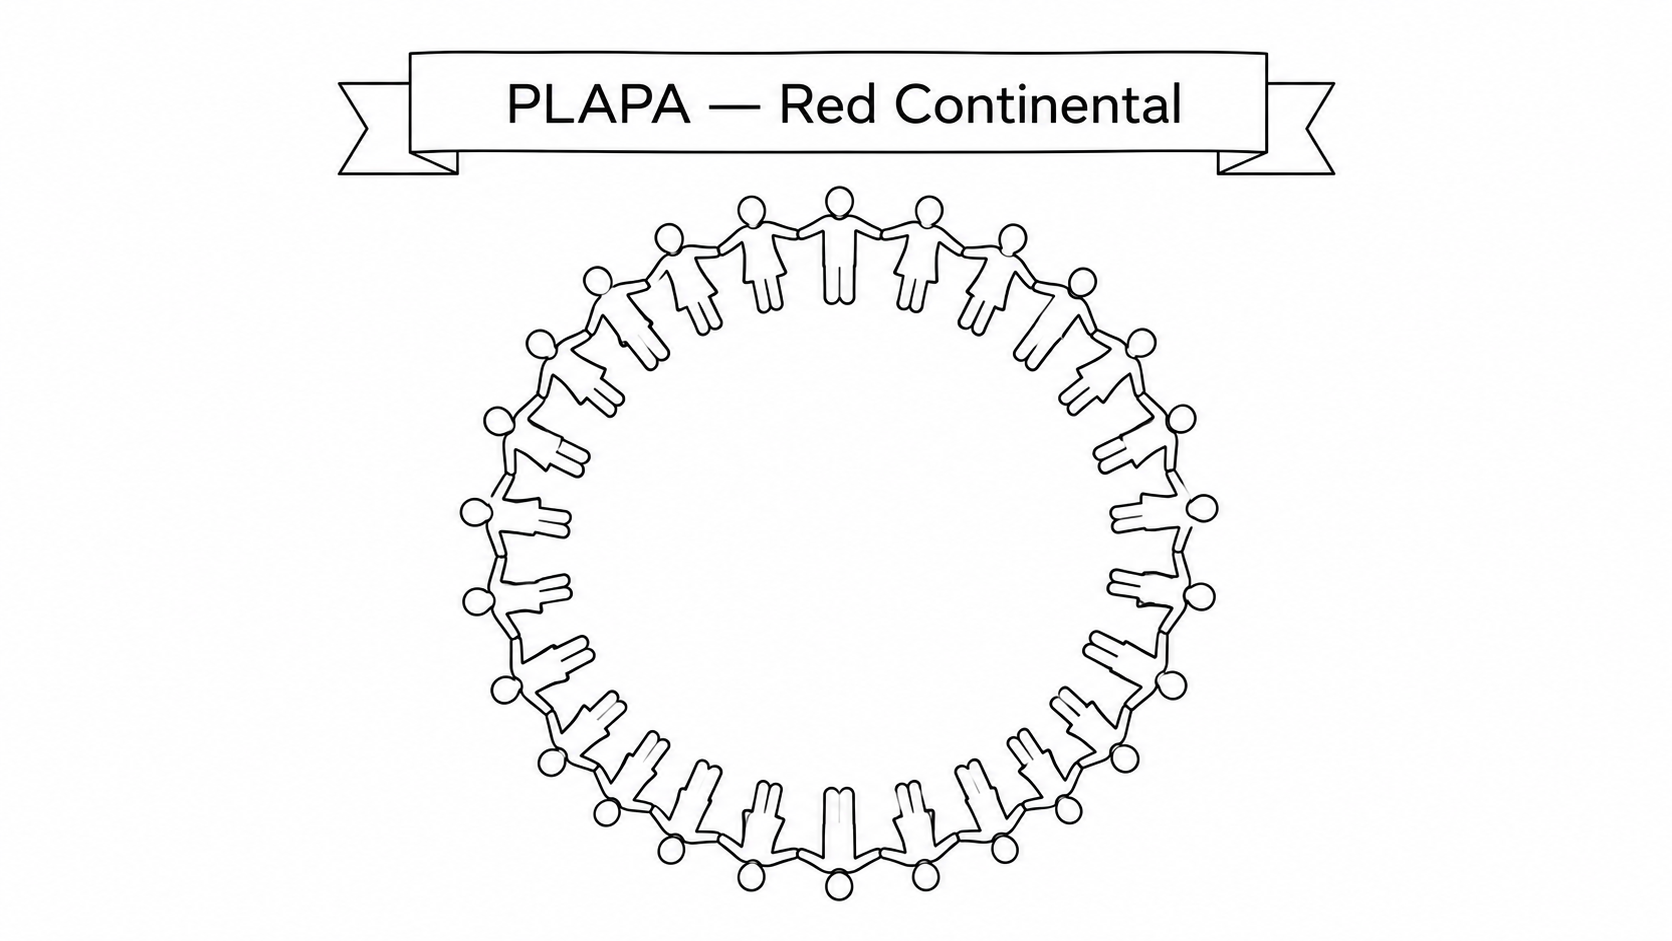
\includegraphics[scale=0.2]{PLAPA.png}
		\caption{Red de experiencias concretas de la PLAPA}
	\end{figure}
	
	
	\section{Catequesis Preventiva}
	
	\begin{fichalateral}
		\small
		\textbf{País:} Uruguay \\
		\textbf{Descripción:} Incorporación de elementos preventivos en los programas de catequesis \\
		\textbf{Contacto: } \texttt{pastoraldeadicciones@caritasuruguaya.org.uy}
	\end{fichalateral}
	
	En la sección de Propuestas pastorales por ámbito (11.1.12), dentro del Ámbito parroquial, hemos desarrollado la propuesta de un abordaje preventivo desde la catequesis. Caritas Uruguaya está implementando a nivel nacional esta propuesta y puede ser motivo de inspiración para otros países. Aquí dejamos su contacto.
	
	\section{La Pastoral de la Sobriedad}
	
	\begin{fichalateral}
		\small
		\textbf{País:} Brasil \\
		\textbf{Descripción:} Red pastoral qeu agrupa grupos de autoayuda, oración y apoyo en todo el país\\
		\textbf{Contacto: } \texttt{cnbb3@sobriedade.org.br}
	\end{fichalateral}
	
	La Pastoral de la Sobriedad nace como una respuesta concreta de la Iglesia en Brasil (CNBB) al desafío lanzado por el Papa San Juan Pablo II de combatir el flagelo de las adicciones. Su misión es evangelizar a través del anuncio de Jesucristo Libertador, promoviendo la dignidad de la persona y de la familia mediante el servicio, el diálogo y el testimonio, haciendo de los excluidos sus preferidos. Ante una cultura que mercantiliza el descarte, esta pastoral responde al llamado bíblico de Deuteronomio 30, 19, transformando la búsqueda de la sobriedad en una opción radical por elegir la vida.\marginnote{Dt 30, 19\label{dt30,19} — \textit{Pongo hoy delante de ti la vida y la muerte, la bendición y la maldición. Elige la vida}}
	
	\subsection{Identidad: El Grupo de Autoayuda (GAA)}
	
	La identidad de esta pastoral reside en la vivencia de los 12 Pasos del Programa de Vida Nueva dentro del Grupo de Autoayuda, un espacio guiado por el lema institucional: «Sobriedad y paz, solo por hoy gracias a Dios». El trabajo del grupo abarca:
	
	\begin{itemize}
		\item \textbf{Dependencias a sustancias lícitas e ilícitas:} alcohol, tabaco y otras drogas.
		\item \textbf{Comportamientos:} mentira, terquedad, rechazo, manías, egoísmo, falta de perdón, de aceptación, entre otros.
		\item \textbf{Trastornos de salud mental:} ansiedad, depresión, fobias, ataques de pánico, entre otros.
		\item \textbf{Compulsiones:} juego, apuestas en línea, compras, tecnologías, codependencia emocional, entre otros.
	\end{itemize}
	
	La fuerza del grupo constituye un recurso eficaz para restaurar el equilibrio emocional, espiritual, social y comunitario a través de la ayuda mutua y de un modelo sistémico y conductual que involucra a toda la familia.
	
	\subsection{El Programa «Nueva Vida»: Los 12 Pasos}
	
	Esta metodología se basa en los 12 pasos: admitir, confiar, entregar, arrepentirse, confesar, renacer, reparar, profesar la fe, orar y vigilar, servir, celebrar y festejar.
	
	El programa no se limita solo a bloquear el uso de sustancias, sino que propone el redescubrimiento de la dignidad y el verdadero sentido de la vida, fomentando la terapia del amor incondicional y el apoyo mutuo. Es un proceso gradual que requiere perseverancia en la búsqueda de la sobriedad y en la conversión de vida a la luz del Evangelio. Así, ofrece un camino de esperanza y transformación para quienes desean liberarse de las ataduras del sufrimiento y vivir plenamente en todas sus dimensiones.
	
	\subsection{Dinámica del Encuentro Pastoral}
	
	La Pastoral de la Sobriedad se diferencia de otros grupos civiles por su carácter explícitamente evangelizador. Sus reuniones semanales siguen una estructura de acogida y oración donde se proclama con fe: «Piedad Redentora de Cristo: danos la sobriedad». El núcleo del encuentro es el Grupo de Autoayuda con las siguientes características:
	
	\begin{itemize}
		\item \textbf{Carácter abierto e inclusivo:} Cualquier persona puede participar. No se limita a las drogodependencias, sino que amplía su alcance a diversos tipos de adicciones, compulsiones, pecados y sufrimientos.
		\item \textbf{Separación por vínculos afectivos:} No se divide a los participantes por su condición o sustancia, sino que se separa a los miembros de una misma familia o personas con lazos afectivos cercanos. El objetivo es evitar confrontaciones, juicios o inhibiciones recíprocas durante el encuentro.
		\item \textbf{Escucha respetuosa:} Se garantiza un espacio seguro donde se puede hablar sin ser juzgado. Está estrictamente prohibido dar consejos, emitir opiniones o interrumpir a quien comparte su testimonio.
		\item \textbf{Confidencialidad:} El secreto y el sigilo absoluto sobre lo compartido en la reunión es la base de la confianza grupal.
		\item \textbf{Terapia del Amor y el Perdón:} Al abrir el corazón y escuchar al otro, los participantes se vuelven sensibles al dolor ajeno, estimulando un cambio en la conducta personal.
	\end{itemize}
	
	\subsection{Frentes de Acción}
	
	La pastoral articula su servicio en cinco frentes estratégicos dentro de la sociedad:
	
	\begin{enumerate}
		\item \textbf{Prevención:} Educación y sensibilización familiar y social para evitar el inicio de dependencias.
		\item \textbf{Intervención:} Acogida inmediata y orientación en momentos de crisis.
		\item \textbf{Recuperación:} El camino de los 12 pasos e integración en la vida comunitaria.
		\item \textbf{Reintegración:} Apoyo para el regreso a la vida familiar, laboral y ciudadana.
		\item \textbf{Acción Política:} Participación e interlocución ante las secretarías de políticas sobre drogas y prevención de adicciones para exigir y ayudar a proponer políticas públicas que respeten la dignidad humana.
	\end{enumerate}
	
	\subsection{El Agente de Sobriedad}
	
	No es un técnico o terapeuta clínico, es un portador de esperanza. Su misión es expresar, con humildad, el amor gratuito del Padre, sirviendo gratuitamente a ejemplo de María, nuestra madre y madre de todos, haciendo de los excluidos los preferidos a través de la Pastoral de la Sobriedad y, como afirma el Papa Francisco, busca combatir esa «prisión invisible» de las dependencias con las herramientas de la fe, la palabra compartida y la vida en comunidad.
	
	
	
	
	\section{Los Hogares de Cristo (Centros Barriales)}
	
	
	\begin{fichalateral}
		\small
		\textbf{País:} Argentina \\
		\textbf{Descripción:} Centros Barriales en las parroquias \\
		\textbf{Contacto: } \texttt{maxfehrmann@hogardecristo.org.ar}
	\end{fichalateral}
	
	
	\textbf{Una respuesta comunitaria y profética desde los barrios populares}\\
	
	La Familia Grande Hogar de Cristo no nace de una planificación técnica, sino de un gesto profundamente evangélico: el lavatorio de los pies. En el Jueves Santo de 2008, el entonces Cardenal Jorge Mario Bergoglio repitió el gesto de Jesús con jóvenes que estaban luchando por salir del consumo. Allí propuso la mística que hoy orienta a cientos de centros barriales: \textit{Recibir la vida como viene y acompañarla cuerpo a cuerpo}\index{mística|textbf}.
	
	Este gesto fundacional, hoy proyectado globalmente por el Papa Francisco, es una toma de posición eclesial: frente a la tentación de lavarse las manos ante el dolor de los excluidos, la Iglesia elige el lugar del servicio. Allí donde el mundo descarta, los Hogares de Cristo revelan que el amor se vuelve presencia y que la Iglesia asume la responsabilidad compartida de no abandonar a nadie en el camino.
	
	\subsubsection{Pilares de la Identidad Pastoral}
	La respuesta de los Hogares de Cristo se basa en una espiritualidad encarnada que se sostiene en tres pilares:
	
	\begin{itemize}
		\item \textbf{Cercanía:} Es\index{cercanía} la decisión de dejarse afectar por el dolor del hermano. Implica poner en el centro a quien la sociedad invisibiliza, permitiendo que su realidad atraviese la propia vida.
		\item \textbf{Presencia:} La cercanía hecha cotidianeidad. Es el estar que da certeza a quienes han vivido la orfandad y el abandono: \textit{puedo contar con ustedes, no se van a borrar}.
		\item \textbf{Vínculo:} De la presencia nace el vínculo y el reconocimiento del nombre. Para los Hogares de Cristo, el paso del estigma al nombre propio -- de ser un anónimo de la calle a ser un hijo de la comunidad -- es el inicio de toda sanación.
	\end{itemize}
	
	\subsubsection{La Comunidad como Territorio de Sanación: Mesa, Casa y Familia}
	Bajo la convicción de que nadie se salva solo, la Familia Grande Hogar de Cristo (FGHC) entiende que el consumo suele ser el síntoma de soledades prolongadas. Por eso, el camino no es solo la abstinencia, sino la reconstrucción de la pertenencia.
	
	\begin{itemize}
		\item \textbf{La Mesa:} No se trata solo de asistir con alimento, sino de sentar al hermano a la mesa, integrándolo como un igual.
		\item \textbf{La Casa:} Los centros barriales son hogares. En la vida compartida -- comer, trabajar, rezar y celebrar juntos -- se reconstruye la dignidad humana.
		\item \textbf{La Familia:} El abordaje es integral. Salud, documentación, educación y fe forman un solo proceso que acompaña a la persona en su totalidad.
	\end{itemize}
	
	\subsubsection{Una Epistemología del Aprendizaje}
	La FGHC propone entrar al territorio como discípulos. Es una pastoral que aprende a decir <<no sé>> y se deja interpelar por la vida del otro. En este horizonte, la recaída no se lee como un fracaso moral, sino como una parte del camino que exige más cercanía. La puerta siempre permanece abierta porque el criterio no es la eficacia, sino la fidelidad del amor.
	
	\subsubsection{Dimensión Profética}
	Finalmente, la FGHC interpela estructuras. Allí donde el mercado de la droga ofrece pertenencia falsa, la Iglesia propone una comunidad que cuida. Es un camino que testimonia que la vida puede renacer cuando es acogida y amada, celebrando cada pequeño brote de vida como un germen de resurrección.
	
	\subsection{La Cooperativa: El pan nuestro de cada día}
	
	
	\begin{fichalateral}
		\small
		\textbf{País:} Argentina \\
		\textbf{Descripción:} Cooperativa de elaboración de alimentos de personas en recuperación  \\
		\textbf{Contacto: } \texttt{pannuestrolamatanza@gmail.com}
	\end{fichalateral}
	
	
	El Pan Nuestro de Cada Día es una cooperativa de trabajo nacida en el camino pastoral del Hogar de Cristo de la Parroquia San José, en La Matanza. No empezó como una empresa ni como un emprendimiento armado desde un escritorio. Nació de una necesidad concreta que aparecía todos los días en el acompañamiento de los centros barriales: muchos chicos y chicas lograban salir de la calle, empezar un proceso de recuperación, volver a una casa o a una comunidad, pero seguían sin una posibilidad real de trabajo.
	
	Al principio la urgencia había sido otra. La comunidad salía a buscar a las personas que estaban en situación de calle. Lo primero fue acercar comida caliente, abrir un lugar donde pudieran descansar, escuchar, acompañar. Después vinieron los espacios más estables del Hogar de Cristo, las casas, los centros barriales, los equipos de acompañamiento. Pero en ese camino apareció una pregunta que no se podía esquivar: ¿cómo sigue la vida de una persona que empieza a recuperarse si no tiene trabajo, rutina ni un lugar donde sentirse necesaria? De esa pregunta nació El Pan Nuestro de Cada Día.
	
	La primera forma fue sencilla: una casa de comidas en el Polideportivo San José, en La Matanza, donde empezaron a trabajar jóvenes del Hogar de Cristo que estaban en recuperación. En 2022, ya trabajaban más de 50 personas, con la posibilidad de proyectar su vida, desarrollarse laboralmente y reintegrarse socialmente. 
	
	Con el tiempo, la experiencia creció. Lo que había empezado como una casa de comidas se fue convirtiendo en una cooperativa con distintas tareas y espacios de trabajo. Hoy El Pan Nuestro de Cada Día combina producción, cocina, atención al público, panificación, reparto, logística, compras, limpieza, mantenimiento y organización cotidiana. En 2025 es una Cooperativa de Trabajo que da trabajo a más de 250 personas en La Matanza, fortalecida en alianza con la Familia Grande Hogar de Cristo. 
	
	La cooperativa no funciona en un solo lugar ni hace una sola tarea. En La Matanza se reconocen distintos espacios vinculados a la experiencia: el Santuario Virgen del Milagro de Caacupé, la Casa de Comidas —donde se sirve diariamente al público— y la Panificadora Colonia Mi Esperanza, donde se elaboran productos. Esa diversidad ayuda a entender mejor la dimensión de la experiencia: no se trata solamente de “hacer pan”, sino de construir una red de trabajo comunitario alrededor de la vida cotidiana del barrio. 
	
	En la panificadora se elaboran productos para vender y distribuir. En la casa de comidas se cocina y se atiende al público. Otros compañeros se ocupan de compras, administración de insumos, reparto, recepción de pedidos, limpieza, mantenimiento de los espacios y organización de los turnos. Algunos tienen más experiencia y enseñan a quienes recién empiezan. Otros están dando sus primeros pasos y necesitan aprender desde lo más básico: llegar a horario, sostener una tarea, cuidar una herramienta, trabajar con otros, avisar cuando no pueden ir, cobrar por su trabajo y administrar algo de dinero.
	
	Esa es una de las claves de la experiencia. El Pan Nuestro de Cada Día no es solamente un emprendimiento productivo. Es parte del proceso de recuperación comunitaria del Hogar de Cristo. Por eso no se organiza únicamente alrededor de la eficiencia o de la productividad. Allí trabajan personas que vienen de situaciones muy difíciles: consumo problemático, calle, cárcel, violencia, abandono, años de exclusión. Algunos siguen vinculados a casas convivenciales, centros barriales o espacios de acompañamiento. Otros ya tienen más recorrido y ayudan a sostener a los nuevos.
	
	La cooperativa funciona como un lugar de trabajo, pero también como una escuela de vida cotidiana. Se aprende un oficio, pero también se recuperan hábitos. Se produce comida, pero también se reconstruyen vínculos. Se trabaja para vender, pero también para que cada compañero vuelva a sentirse parte de algo.
	
	Muchas comunidades tienen talleres, roperos, ferias, cursos o pequeñas producciones solidarias. Todo eso tiene mucho valor. Pero en El Pan Nuestro de Cada Día el trabajo no aparece como una actividad paralela a la pastoral ni como una ayuda para sostener una obra. El trabajo está metido adentro del camino de recuperación. Es una herramienta concreta para que una persona pueda volver a ordenar su día, recuperar confianza, asumir responsabilidades y sentirse necesaria para los demás.
	
	La experiencia también muestra que la inclusión laboral no se logra solamente consiguiendo máquinas o insumos. Hace falta una comunidad que acompañe. Por eso, junto con el equipamiento y la capacitación, son fundamentales la presencia cotidiana, la escucha, la paciencia, la organización y la capacidad de volver a empezar cuando algo no sale bien. 
	
	Como en toda experiencia real, no todo es prolijo ni fácil. Hay días en que faltan ventas, se rompe una máquina, alguien no llega, aparecen conflictos o un compañero recae. Pero la lógica no es descartar al que no puede. La lógica es comunitaria: hablar, sostener, ordenar, volver a intentar. Esa paciencia es parte del método.
	
	Para una parroquia que quiera comenzar algo parecido, la enseñanza principal es que no hace falta empezar grande. El Pan Nuestro de Cada Día comenzó desde una necesidad concreta y fue creciendo paso a paso. Primero una comunidad que sale a buscar, escucha y acompaña. Después una tarea posible: cocinar, amasar, vender, repartir. Luego una organización más estable. Más adelante, capacitación, equipamiento, articulaciones y nuevas unidades productivas.
	
	Lo decisivo no es copiar exactamente una panadería o una casa de comidas. Lo decisivo es comprender el método: que el trabajo sea parte del acompañamiento, que los protagonistas sean los propios compañeros, que la comunidad sostenga el proceso y que la producción esté al servicio de reconstruir vidas.
	
	En el Hogar de Cristo se suele decir que nadie se recupera solo. El Pan Nuestro de Cada Día muestra una forma concreta de hacer verdadera esa frase: una mesa, una cocina, una panificadora, un reparto, un turno de trabajo, una comunidad que confía y muchos compañeros que, mientras producen el pan de cada día, vuelven a encontrar un lugar en la vida.
	
	
	
	\subsection{La Cooperativa de Acompañantes AUPA}
	
	\begin{fichalateral}
		\small
		\textbf{País:} Argentina \\
		\textbf{Descripción:} Cooperativa de acompañantes en los procesos de recuperación e integración\\
		\textbf{Contacto: } \texttt{cooperativaaupa@hogardecristo.org.ar}
	\end{fichalateral}
	
	
	
	La Cooperativa de Trabajo de Acompañantes de Usuarios de Paco Limitada (AUPA), nacida en 2011 en la Villa 21-24 y el NHT Zavaleta (CABA), constituye un modelo de inclusión social por la vía laboral que desafía los esquemas convencionales de asistencia. Inscripta ante el INAES (Matrícula 48.298) en septiembre de 2013, opera bajo la órbita de la Federación Familia Grande Hogar de Cristo y articula de forma directa con la Parroquia Nuestra Señora de Caacupé. La propuesta demuestra que el cuidado de las personas más vulnerables es indisociable de la organización colectiva y de la dignificación de quienes cuidan.
	
	
	\textbf{Población Objetivo:} Personas usuarias de pasta base de cocaína en la Ciudad de Buenos Aires y el conurbano bonaerense, acompañadas desde su primer pedido de ayuda hasta su inclusión social efectiva. 
	
	\textbf{Pilares de la Propuesta Cooperativa:}
	\begin{itemize}
		\item \textit{El trabajo como vínculo:} Los acompañantes no ejecutan un protocolo frío; habitan el territorio y sostienen una presencia cotidiana, transformando el trabajo cooperativo en la modalidad terapéutica misma.
		\item \textit{Inclusión recíproca:} Muchos asociados son personas recuperadas en los Centros Barriales del Hogar de Cristo; la cooperativa dignifica su trayectoria de vida al transformarlos en trabajadores del cuidado de otros.
		\item \textit{Formación autogestiva:} La participación horizontal en asambleas y la toma de decisiones colectivas fortalecen capacidades humanas y corresponsabilidad comunitaria más allá del oficio laboral.
	\end{itemize}
	
	
	
	\subsubsection{Síntesis del Modelo}
	\textit{La experiencia de AUPA ofrece una respuesta replicable para América Latina frente al fracaso de los servicios sociales tradicionales. Demuestra que cuando las instituciones formales no alcanzan a las periferias, la comunidad organizada puede constituirse en sujeto colectivo de cuidado. La forma cooperativa brinda el marco jurídico e institucional necesario para garantizar derechos laborales, responsabilidades compartidas y sustentabilidad en el tiempo, transformando el dolor en trabajo digno y organización comunitaria.}
	
	
	\subsection{Propuesta de las 3 T: Tierra, Techo y Trabajo (Barrio Comunitario)}
	
	
	\begin{fichalateral}
		\small
		\textbf{País:} Argentina \\
		\textbf{Descripción:} Comunidad donde viven y trabajan personas en recuperación \\
		\textbf{Contacto: } \texttt{3tmarcospaz@gmail.com}
	\end{fichalateral}
	
	
	Inspirada en el llamado del Papa Francisco a organizarse en torno a los Derechos Sagrados de todo ser humano, la propuesta de las 3 T (\textit{Tierra, Techo y Trabajo}) constituye una respuesta estructural y de largo plazo frente a la pobreza y la exclusión social. Partiendo del abrazo primario en el territorio (calle, comida, higiene) desarrollado en los Centros Barriales del \textbf{Hogar de Cristo}, este modelo avanza hacia la consolidación de un \textbf{Barrio Comunitario} en zonas rurales. Este dispositivo propone un proceso inverso de migración (de la ciudad al campo) para familias que buscan un cambio radical de vida, alejadas de la violencia y el consumo de las villas de emergencia.
	
	\subsubsection{Los Tres Ejes Sagrados del Desarrollo Humano}
	La organización del Barrio Comunitario se estructura directamente sobre los tres pilares de las 3 T:
	\begin{itemize}
		\item \textbf{Trabajo (Dignidad y Cooperativismo):} Funciona como un proceso de reconstrucción de la cultura del trabajo para quienes están excluidos del sistema laboral formal. Bajo una lógica cooperativa, asamblearia y de discernimiento comunitario, los esfuerzos se orientan principalmente a la \textbf{producción agroecológica de alimentos} (carne, leche, huevos, vegetales, miel) para combatir el hambre y la desigualdad nutricional. Asimismo, incluye economías del cuidado ambiental como el reciclaje, confección de jabones y elaboración de conservas.
		\item \textbf{Techo (Vivienda y Estabilidad Vincular):} El acceso al techo propio se divide en dos etapas claves durante un proceso estimado de dos años: una primera fase de alojamiento transitorio en espacios comunitarios para internalizar los acuerdos del barrio, y una segunda fase de acompañamiento en la autoconstrucción. Esta última se financia mediante un sistema de \textbf{microcréditos} que activa la mano de obra local. La vivienda propia impacta de forma directa en la reducción de las violencias (intrafamiliar y de género) y de esta manera estabiliza las trayectorias escolares, terapéuticas y los proyectos de vida.
		\item \textbf{Tierra (Laudato Si\label{lsb} y Cuidado de la Casa Común):} Frente a las realidades de exclusión en barrios que lindan con basurales, la vida en la naturaleza se asume como un espacio de sanación profunda y conexión espiritual. Se implementa una educación ambiental continua y práctica: sistemas de desagüe sustentables, gestión agroecológica de plagas y reciclaje integral. Los referentes más antiguos asumen el rol de guiar a los recién llegados en las pautas de cuidado del entorno.
	\end{itemize}
	
	\subsubsection{Comunidad Organizada y Abordaje de la Complejidad}
	El sostenimiento de la autonomía en el barrio no se da de forma aislada, sino a través de una red de lazos y contenciones comunitarias e institucionales preparadas para absorber la alta complejidad:
	\begin{itemize}
		\item \textbf{Equipos Terapéuticos Integrados:} Profesionales de la salud y referentes barriales coexisten y trabajan de forma articulada en el territorio, garantizando espacios de escucha individual diaria, asambleas convivenciales y abordajes pedagógicos.
		\item \textbf{Gestión de Crisis y Salud Mental:} La comunidad cuenta con dispositivos específicos para acompañar recaídas en el consumo, crisis de salud mental graves y articulación de personas con causas penales o conflictos con la ley, evitando la exclusión punitiva.
		\item \textbf{Crianza y Entorno Comunitario:} La resolución de conflictos se gestiona mediante acuerdos colectivos explícitos, promoviendo espacios compartidos para el desarrollo de las infancias y las adolescencias en un ambiente libre de violencia.
	\end{itemize}
	
	\subsubsection{Síntesis del Modelo}
	\textit{La Comunidad de las 3 T se consolida como un faro de esperanza y arraigo de justicia social. Al fusionar la mística de la comunidad organizada con el saber profesional, transforma las historias de descarte y oscuridad en testimonios de sanación, demostrando que la restitución de los derechos sagrados a la Tierra, el Techo y el Trabajo es el camino definitivo hacia la dignidad humana.}
	
	\subsection{Casa Masantonio: Salud Comunitaria en Extrema Vulnerabilidad}
	
	\begin{fichalateral}
		\small
		\textbf{País:} Argentina \\
		\textbf{Descripción:} Hospital para personas usuarias de pasta base, vida en calle y enfermedades infectocontagiosas (VIH, TBC, etc.) \\
		\textbf{Contacto: } \texttt{casamasantonio@gmail.com}
	\end{fichalateral}
	
	
	La Casa Masantonio (con más de 10 años de trayectoria) es un dispositivo de acompañamiento territorial con foco en la salud pública y de base comunitaria. Pertenece a la Cooperativa de Acompañantes de Usuarios de Paco (AUPA) dentro de la Federación Familia Grande Hogar de Cristo, y se encuentra íntimamente vinculada a la pastoral de la Parroquia Virgen de Caacupé (Villa 21-24 y Zabaleta, CABA, Argentina). Nace como un dispositivo emancipador y de resistencia frente a la deshumanización y la crueldad organizada que margina a los más descartados de la sociedad.
	
	\subsubsection{Justificación: La Brecha del Sistema Sanitario Formal}
	La mayor carga de enfermedad en las personas en extrema vulnerabilidad social y consumo problemático de pasta base de cocaína (<<paco>>) corresponde a patologías prevenibles y tratables (Tuberculosis, VIH en estadios avanzados, neumonías agudas e infecciones respiratorias). Cuando se presenta una enfermedad grave, la ventana de oportunidad para salvar la vida es biológicamente estricta y no responde a los tiempos subjetivos del tratamiento de las adicciones; es una carrera contrarreloj.
	
	El sistema de salud formal fragmenta a la persona y presupone erróneamente que el paciente tiene resueltos los determinantes sociales básicos (alimentación, techo, capacidad económica para adquirir medicamentos, transporte y estabilidad psíquica para sostener un turno médico). Al carecer de una \textbf{red de cuidados continuos}, los abordajes hospitalarios tradicionales fracasan sistemáticamente, empujando a los usuarios a la interrupción de tratamientos y a muertes extremadamente prematuras.
	
	\subsubsection{Metodología de Acompañamiento <<Cuerpo a Cuerpo>>}
	Frente a la atención clínica puntual y aislada, Casa Masantonio interpone una clínica de la vulnerabilidad situada que opera bajo los siguientes ejes metodológicos:
	\begin{itemize}
		\item \textbf{Acompañantes Pares:} La estrategia es sostenida por referentes territoriales y pares que han atravesado realidades similares. Esto elimina la asimetría del poder médico tradicional, construyendo un puente de confianza indispensable para la adherencia terapéutica.
		\item \textbf{Red de Cuidados Integrales:} La administración del tratamiento farmacológico se inserta dentro de la cobertura de las necesidades humanas más básicas. Curar la enfermedad exige, simultáneamente, garantizar un plato de comida, abrigo, una ducha digna, espacios de descanso seguros y acompañamiento afectivo.
		\item \textbf{Gestión de la Complejidad Médica en Territorio:} Articulación directa con el Estado y efectores hospitalarios para la facilitación de turnos, seguimiento clínico, provisión de esquemas de medicación compleja (como el Tratamiento Acortado Estrictamente Supervisado - DOTS para Tuberculosis) y acompañamiento en internaciones.
	\end{itemize}
	
	\subsubsection{Evidencia Científica de Efectividad y Éxito Terapéutico}
	El modelo de Casa Masantonio ha dejado de ser solo una <<experiencia pastoral novedosa>> para consolidarse como una tecnología social de salud pública validada internacionalmente. Un estudio de cohorte retrospectivo (periodo 2019-2023) publicado en la \textit{Revista Panamericana de Salud Pública} de la Organización Panamericana de la Salud (OPS/OMS) arrojó resultados contundentes sobre la efectividad del dispositivo en una población de altísima vulnerabilidad (donde el 55\% se encontraba en situación de calle efectiva y el 77\% bajo consumo problemático de sustancias):
	\begin{itemize}
		\item \textbf{Éxito Terapéutico en Tuberculosis:} Alcanzó un \textbf{93, 8\%} de éxito en la curación y finalización de tratamientos, en comparación con el 70, 2\% registrado en la población general del Área Metropolitana de Buenos Aires (AMBA).
		\item \textbf{Reducción del Abandono (Pérdida de seguimiento):} Se desplomó drásticamente a solo un \textbf{2, 1\%}, frente al alarmante 19, 9\% del sistema de salud convencional.
		\item \textbf{Disminución de la Mortalidad:} Registró una tasa de mortalidad notablemente menor respecto de la media habitual para este perfil de pacientes (4, 1\% en Casa Masantonio frente a un 9, 7\% en las estrategias habituales de atención).
	\end{itemize}
	
	\subsubsection{Síntesis del Modelo}
	\textit{La propuesta de Casa Masantonio demuestra que para obtener éxito en el tratamiento de enfermedades complejas en contextos de exclusión, es biológica y socialmente indispensable integrar el saber profesional con el acompañamiento comunitario y territorial. Acompañar la salud <<cuerpo a cuerpo>> no solo restituye el bienestar físico y evita los contagios epidemiológicos en los barrios populares, sino que devuelve de manera primordial el rostro humano y la dignidad a los más rotos de los rotos.}
	
	\subsection{Espacio SumaySimi: Abordaje Comunitario de Padecimientos Mentales Graves}
	
	\begin{fichalateral}
		\small
		\textbf{País:} Argentina \\
		\textbf{Descripción:}  Programa para usuarios de pasta base con padecimientos mentales severos y extrema vulnerabilidad social\\
		\textbf{Contacto: } \texttt{cooperativaaupa@hogardecristo.org.ar}
	\end{fichalateral}
	
	
	El Espacio <<SumaySimi>> (del quechua: \textit{Sumay}, calma; \textit{Simi}, hablar; calmarse al encontrarse y ser escuchado) nació en abril de 2019 bajo la órbita de la Cooperativa AUPA y la Familia Grande Hogar de Cristo en la Villa 21-24 y el NHT Zavaleta. Este dispositivo surge para dar respuesta a una realidad compleja que desborda los protocolos tradicionales: personas en situación de calle con consumo problemático de pasta base que presentan, simultáneamente, padecimientos mentales graves y/o discapacidades físicas e intelectuales.
	
	\begin{itemize}[leftmargin=*]
		\item \textbf{Justificación (La Doble Exclusión):} Esta población sufre una marginación absoluta, ya que no accede a hospitales psiquiátricos por su situación de calle y consumo, es rechazada en centros de adicciones comunes por la gravedad de su cuadro psiquiátrico, y es expulsada de los paradores por problemas conductuales. El dispositivo interviene directamente sobre esta comorbilidad\index{comorbilidad!y situación de calle} para reducir la cronicidad y la mortalidad.
		
		\item \textbf{Sedes y Modalidades de Atención:} El programa distribuye su acompañamiento en dos sedes estratégicas en CABA:
		\begin{itemize}
			\item \textit{Sede Ambulatoria (Casa GESA, Barracas):} Funciona de lunes a viernes en turno diurno, brindando soporte y seguimiento a más de 100 personas.
			\item \textit{Vivienda Comunitaria (Casa SumaySimi, Pompeya):} Residencia permanente con cobertura 24/7 y capacidad para 20 personas, proporcionando la estabilidad habitacional indispensable para viabilizar cualquier proceso terapéutico.
		\end{itemize}
		
		\item \textbf{Ejes Operativos de la Propuesta:}
		\begin{itemize}
			\item \textit{Atención clínica integral:} Equipo interdisciplinario (psiquiatras, psicólogos, trabajadores sociales y operadores) que realiza psicoterapias, controles de salud física y el suministro estrictamente supervisado de psicofármacos.
			\item \textit{Laborterapia y oficios:} Talleres de carpintería, herrería y jardinería con un doble fin: terapéutico (reorganización de la rutina y rehabilitación de funciones cognitivo-ejecutivas) y formativo para la inclusión laboral.
			\item \textit{Acompañamiento par:} Incorporación de personas recuperadas del consumo como protagonistas del equipo, cuya experiencia testimonial y territorial mejora la adherencia y reduce recaídas.
		\end{itemize}
		
		\item \textbf{Principios Replicables para la Comunidad:} El modelo propone cuatro acciones aplicables a cualquier territorio parroquial o centro barrial:
		\begin{enumerate}
			\item \textit{Identificar sin descartar:} Detectar cuadros de dualidad psiquiátrica en el barrio y no derivarlos a ciegas, manteniendo el lazo y caminando junto a ellos.
			\item \textit{Estructurar el trabajo:} Utilizar los talleres de oficio como herramientas de rehabilitación clínica del deterioro cognitivo y no como un mero pasatiempo.
			\item \textit{Profesionales en salida:} Articular con psicólogos y psiquiatras dispuestos a romper la lógica del consultorio para intervenir directamente en el territorio.
			\item \textit{Validar al par:} Formalizar y rentar el rol del acompañante par por su legitimidad única para construir confianza.
		\end{enumerate}
	\end{itemize}
	
	\subsubsection{Síntesis del Modelo}
	\textit{SumaySimi demuestra que la amorosidad comunitaria y la técnica profesional se necesitan mutuamente para humanizar la salud mental. No se trata de un centro clínico con espiritualidad agregada, sino de una verdadera familia que recibe la vida como viene, cuerpo a cuerpo y sin condiciones previas, logrando que quienes no cabían en ningún sistema encuentren, por fin, un espacio de pertenencia, sanación y dignidad.}
	
	
	\subsection{Las Casas Libertad}
	
	\begin{fichalateral}
		\small
		\textbf{País:} Argentina \\
		\textbf{Descripción:}  Programa para personas privadas de la libertad o liberadas, con vulnerabilidad social grave\\
		\textbf{Contacto: } \texttt{cooperativaaupa@hogardecristo.org.ar}
	\end{fichalateral}
	
	
	Las Casas Libertad surgen en el marco de la red de los Hogares de Cristo. Desde ese espíritu pastoral, las Casas Libertad acompañan a personas atravesadas por el consumo problemático de sustancias, la exclusión social y el sistema penal, poniendo en el centro el vínculo, la dignidad y la esperanza.  
	
	La propuesta se sostiene en una convicción sencilla pero profunda: la libertad no se construye solamente con leyes o decisiones individuales, sino con comunidad, tiempo y cuidado. Por eso, las Casas Libertad no trabajan aisladas ni “contra” el Estado, sino articulando con organismos penitenciarios, judiciales y sociales, aportando una presencia humana y territorial allí donde muchas veces predominan la fragmentación, la burocracia o el abandono.  
	
	El trabajo se desarrolla en tres grandes campos de acompañamiento:
	
	\begin{enumerate}
		
		\item El acompañamiento en contextos de encierro.
		
		Las Casas Libertad acompañan a personas privadas de libertad a través de visitas, escucha, asistencia concreta y sostén vincular. La tarea no se limita a \textit{ir a la cárcel}, sino a sostener la vida allí donde el encierro suele profundizar la soledad y la desesperanza. Se trabaja desde la cercanía, muchas veces con acompañantes pares —personas que también atravesaron situaciones de consumo, cárcel o exclusión— mostrando que el cambio es posible. La espiritualidad está presente como horizonte de sentido y esperanza, siempre desde una lógica abierta y no impuesta.  
		
		\item El acompañamiento post-penitenciario
		
		La salida de la cárcel no es entendida como el final del problema, sino como el comienzo de una etapa frágil y decisiva. Las Casas Libertad sostienen espacios convivenciales y comunitarios donde las personas puedan reconstruir hábitos, vínculos y proyectos de vida. Desde una \textit{pedagogía de la libertad}, se aprende a vivir sin consumo, sin violencia y sin delito, no desde el castigo sino desde el cuidado mutuo, la convivencia y la responsabilidad compartida. El trabajo, la vivienda y la comunidad son vistos como derechos fundamentales para que la libertad sea real.  
		
		\item El acompañamiento jurídico-penal
		
		Las Casas Libertad también acompañan el acceso a la justicia de personas que suelen quedar perdidas dentro del sistema judicial. Muchas veces se trata de personas con múltiples causas, sin comprensión de sus procesos judiciales ni posibilidades reales de sostener medidas alternativas. Allí el acompañamiento busca \textit{humanizar} la justicia: traducir, orientar, sostener y construir puentes entre la persona, su comunidad y las instituciones. El derecho no aparece separado de la vida concreta, sino vinculado al territorio, al vínculo y a las posibilidades reales de transformación.  
		
	\end{enumerate}
	
	
	En síntesis, las Casas Libertad buscan sostener procesos de transformación reales, entendiendo que nadie cambia solo y que incluso en las historias más dañadas sigue existiendo una posibilidad de reconstrucción. Más que un dispositivo, es una comunidad organizada que acompaña la vida antes, durante y después del encierro, apostando a una sociedad que no descarte personas y que se anime a cuidar.
	
	\subsection{Emprendimientos Comunitarios}
	
	A diferencia de la lógica corporativa del mercado tradicional ---caracterizada por la competencia individualista, la acumulación y el descarte de los eslabones más débiles---, el emprendimiento en el marco de la economía social y solidaria nace estrictamente del \textit{nosotros}. Se define como la puesta en común de voluntades, fuerzas de trabajo, saberes y habilidades de un grupo de personas que integran una comunidad, con el objetivo explícito de mejorar la calidad de vida y el desarrollo socioeconómico de todos sus participantes.
	
	El método de acompañamiento en nuestros Centros Barriales contempla una transición gradual y cuidada a través de tres dispositivos fundamentales:
	\begin{itemize}
		\item \textbf{La laborterapia:} Es el trabajo que permite conectarse con uno mismo
		\item \textbf{El Taller Parroquial / Espacio Formativo:} Es la instancia inicial donde los jóvenes y adultos recuperan o incorporan hábitos cotidianos elementales (la rutina horaria, el cuidado de las herramientas, la escucha de consignas, el trabajo en equipo y la tolerancia a la frustración). Aquí el objetivo primordial no es la rentabilidad, sino la revinculación y el descubrimiento de las potencialidades individuales.
		\item \textbf{La Unidad Productiva (UP):} Constituye la evolución organizativa del taller hacia un proyecto social autosustentable estructurado para la producción y comercialización formal de bienes o servicios. Requiere una distribución clara de roles (quién produce, quién administra los gastos, quién gestiona los pedidos y la logística) y un registro económico estricto de ingresos y egresos.
	\end{itemize}
	
	En esta estructura, el trabajo está metido adentro del camino de recuperación. La paciencia comunitaria se convierte en método: cuando un compañero atraviesa una crisis o una recaída, la comunidad organizada no lo expulsa ni lo descarta, sino que abre espacios de asamblea, diálogo y discernimiento para reordenar el proceso y volver a intentar. El fin último de estos emprendimientos es demostrar que la autosuficiencia de los sectores vulnerables es posible cuando está sostenida por una red comunitaria afectiva y constante.
	
	\section{Microcréditos y Finanzas Solidarias}
	
	\begin{fichalateral}
		\small
		\textbf{País:} Argentina \\
		\textbf{Descripción:}  Programa microcréditos y educación financiera para personas en recuperación\\
		\textbf{Contacto: } \texttt{ecosol@caritas.org.ar}
	\end{fichalateral}
	
	
	Las Finanzas Solidarias representan la operativización de una economía que sirve a la vida de las personas y dice \textit{<<NO a una economía de exclusión e inequidad donde el dinero reina en lugar de servir>>}. En los territorios de exclusión, el acceso al sistema bancario y crediticio formal está completamente vedado debido a las exigencias burocráticas y patrimoniales. Ante este escenario, la estrategia de los \textbf{Fondos Rotatorios} impulsada por Cáritas y el Hogar de Cristo se presenta como una alternativa basada exclusivamente en la projimidad\index{projimidad!y finanzas solidarias} y la confianza recíproca.
	
	Un Fondo Rotatorio es un instrumento de préstamo comunitario donde el dinero circula de manera transparente: cuando un emprendedor o cooperativa devuelve su crédito, ese mismo recurso se utiliza de inmediato para financiar el proyecto de otro compañero del barrio. Esta dinámica asegura dos principios rectores fundamentales:
	\begin{enumerate}
		\item \textbf{Circularidad:} No existe la acumulación especulativa ni el interés usurero; hay un flujo constante de beneficios que retorna a la base comunitaria.
		\item \textbf{Garantía Solidaria:} El compromiso y el aval del grupo o del Centro Barrial sostienen y respaldan el cumplimiento de cada integrante, transformando el pago de la cuota en un acto de responsabilidad colectiva para con los demás.
	\end{enumerate}
	
	\subsection{Líneas Estratégicas de Financiamiento}
	Los microcréditos se destinan de manera específica a cuatro dimensiones del fortalecimiento productivo:
	\begin{itemize}
		\item \textbf{Compra de Insumos:} Adquisición de la materia prima indispensable para iniciar o garantizar la continuidad de la producción sin depender de intermediarios abusivos.
		\item \textbf{Maquinaria y Herramientas:} Equipamiento técnico que permite mejorar la escala, los costos y la calidad del trabajo, acelerando los procesos de autosuficiencia.
		\item \textbf{Mejoramiento del Espacio:} Arreglos de infraestructura, adecuación de talleres o acondicionamiento de áreas de comercialización y ferias. En contextos periurbanos o rurales, muchas veces este ítem impacta directamente en la mejora de la vivienda familiar.
		\item \textbf{Fortalecimiento Técnico:} Financiamiento para capacitaciones específicas en administración eficiente, diseño, marketing socio-comunitario y uso de redes sociales para la venta.
	\end{itemize}
	
	\subsection{Guía Metodológica para el Acompañamiento Integral}
	Para que las finanzas solidarias cumplan su rol transformador, el equipo interdisciplinario del dispositivo territorial debe aplicar una guía de tres pasos esenciales, bajo la premisa de que \textbf{no se le presta dinero a un número impersonal, sino que se apoya un proyecto de vida:}
	
	\begin{description}
		\item[1. Identificación:] Escuchar atentamente la necesidad real del emprendedor o la cooperativa en el territorio. Evaluar de forma conjunta la viabilidad y el potencial productivo del proyecto, asegurando que la persona cuente con los apoyos necesarios en materia de salud, documentación civil y estabilidad habitacional.
		\item[2. Formulación:] Acompañar técnicamente al participante para plasmar su idea en un plan concreto y ordenado de ingresos, egresos y cálculo de costos, determinando con realismo el monto del microcrédito y un esquema de cuotas de devolución sustentable.
		\item[3. Seguimiento:] Realizar visitas periódicas y presenciales al espacio de trabajo. Este paso es tanto técnico como humano; implica celebrar los logros comerciales del emprendimiento, brindar herramientas administrativas en el campo de acción y ajustar las dificultades operativas o personales antes de que pongan en riesgo el proceso.
	\end{description}
	
	
	\section{Centro de Reintegración Social <<Fortaleza>>}
	
	\begin{fichalateral}
		\small
		\textbf{País:} Bolivia \\
		\textbf{Descripción:}  Instituto penal para menores con enfoque restaurativo\\
		\textbf{Contacto: } \texttt{centro.fortaleza@hotmail.com}
	\end{fichalateral}
	
	
	El Centro de Reintegración Social <<Fortaleza – San Guillermo de Malavalle>> atiende a adolescentes de 14 a 18 años (extensible hasta los 20) bajo medidas judiciales en Bolivia. Implementa un modelo socioeducativo y restaurativo gestionado exclusivamente por personal civil, sin presencia policial, situando el eje del proceso en la dignidad y la transformación del joven.
	
	\begin{itemize}
		\item \textbf{Contexto de Vulnerabilidad:} Los jóvenes provienen de zonas periféricas de alta exclusión. Sus trayectorias están marcadas por deserción escolar, analfabetismo, violencia intrafamiliar, situación de calle y un consumo problemático de sustancias (marihuana y <<piedra>>) estrechamente vinculado a conductas infractoras.
		\item \textbf{Abordaje Multidisciplinario Intramural:} Un equipo interdisciplinario (educadores, psicólogos, trabajadores sociales, pedagogos) coordina de forma diaria espacios clave:
		\begin{itemize}
			\item Talleres de convivencia, fortalecimiento emocional y educación sexual gradual.
			\item Prevención de recaídas y diseño participativo de un plan de vida autónomo.
			\item Educación curricular obligatoria y capacitación técnica/artística (electricidad, computación, música).
		\end{itemize}
		\item \textbf{Desafíos de la Intervención:} El dispositivo trabaja sobre la resistencia y desconfianza inicial del adolescente, la fragilidad o ausencia de contención en sus familias de origen, la baja autoestima y la necesidad de contar con más recursos humanos especializados.
		\item \textbf{Sostenibilidad Post-Egreso:} Para mitigar el riesgo del retorno a entornos de exclusión, el centro implementa el programa \textbf{<<Acompañando en el Retorno>>}, el único dispositivo de post-egreso en Bolivia que brinda seguimiento técnico y contención en la transición del joven hacia el medio libre.
		\item \textbf{Justicia Restaurativa y Redes:} Promueve la articulación con redes comunitarias, educativas y pastorales para desmantelar la estigmatización social, orientando el horizonte hacia una justicia que invita al joven a asumir la responsabilidad del daño causado, reparar sus vínculos y reconciliarse con su comunidad.
	\end{itemize}
	
	\subsection{Síntesis del Modelo}
	\textit{La propuesta del Centro Fortaleza demuestra que es posible sustituir el control punitivo tradicional por una escuela de vida y oportunidades reales. A través de un acompañamiento civil cercano y un programa pionero de post-egreso, el modelo devuelve la dignidad, la palabra y el porvenir a los jóvenes históricamente excluidos.}
	
	
	\section{El abordaje en el ámbito de la carcelación}
	
	\begin{fichalateral}
		\small
		\textbf{País:} Argentina\\
		\textbf{Descripción:}  \\
		\textbf{Contacto: } \texttt{pastoralcarcelariasinfronterap@gmail.com}
	\end{fichalateral}
	
	
	En la sección de Propuestas pastorales por ámbito (11.5), dentro del Ámbito de la carcelación, hemos desarrollado la propuesta de un abordaje de acompañamiento en las cárceles. La Pastoral Carcelaria Argentina está implementando esta propuesta y puede ser motivo de inspiración para otros países. Aquí dejamos su contacto.
	
	\section{La Fazenda da Esperança}
	
	\begin{fichalateral}
		\small
		\textbf{País:} Brasil (y otros países) \\
		\textbf{Descripción:}  Comunidad de vida para la recuperación de personas en situación de dependencia\\
		\textbf{Contacto: } \texttt{secretaria.presidencia@fazenda.org.br}
	\end{fichalateral}
	
	La Fazenda da Esperança es una propuesta de recuperación inspirada en la vivencia cotidiana del Evangelio.
	
	La metodología desarrollada por la Fazenda no se orienta exclusivamente a la abstinencia del consumo de sustancias psicoactivas, sino que contempla un proceso integral de reconstrucción de la persona. Desde esta perspectiva, se comprende que la adicción afecta no solamente la dimensión física, sino también los vínculos afectivos, la estabilidad emocional, la vida espiritual y la capacidad de integración social y comunitaria. En consecuencia, la recuperación se lleva adelante mediante una experiencia concreta de convivencia fraterna, trabajo y espiritualidad.
	
	La dinámica cotidiana dentro de la comunidad tiene como finalidad favorecer el proceso de reconciliación de la persona consigo misma, con los demás y con Dios. El itinerario terapéutico y formativo se desarrolla de manera gradual, respetando los tiempos individuales y reconociendo las particularidades, heridas y desafíos presentes en cada historia personal.
	
	El proceso se inicia con la acogida. La persona es recibida desde el reconocimiento de su dignidad humana, su historia y su potencial de recuperación, evitando toda forma de estigmatización o reducción de su identidad al problema de la adicción. Desde el comienzo se promueve una experiencia comunitaria orientada al redescubrimiento de valores fundamentales como la confianza, el respeto mutuo y la responsabilidad compartida.
	
	La convivencia diaria constituye uno de los pilares esenciales de la propuesta. El compartir la vida con otros hermanos en proceso de recuperación posibilita la confrontación personal, el reconocimiento de límites y la construcción de nuevas formas de relación interpersonal. De esta manera, la comunidad se configura como un espacio terapéutico, educativo y espiritual que favorece la superación del aislamiento y la reconstrucción del sentido de pertenencia.
	
	El trabajo ocupa igualmente un lugar central dentro del proceso de recuperación, siendo comprendido como un instrumento pedagógico y terapéutico. A través de las tareas cotidianas —entre ellas la agricultura, la cocina, la limpieza, la panadería, el cuidado de animales, el mantenimiento y otros servicios comunitarios— la persona redescubre el valor del esfuerzo, la disciplina, el compromiso y la utilidad social. Asimismo, el trabajo contribuye a la reorganización de la vida interior y al fortalecimiento de la autoestima, frecuentemente deteriorada por años de consumo, exclusión y sufrimiento.
	
	La espiritualidad constituye el núcleo fundamental de la experiencia de la Fazenda. La comunidad propone la vivencia concreta de la Palabra de Dios, especialmente mediante la práctica de la denominada \textit{Palabra de Vida}, a través de la cual se procura vivir diariamente un versículo del Evangelio en las situaciones ordinarias de la convivencia. En este sentido, la espiritualidad no se limita a una dimensión teórica o doctrinal, sino que se expresa en actitudes concretas de transformación personal y comunitaria.
	
	Dentro de este proceso integral también se trabajan aspectos fundamentales para la recuperación y reintegración de la persona, tales como:
	
	
	\begin{itemize}
		\item el reconocimiento de la propia fragilidad y de la necesidad de ayuda;
		\item la aceptación responsable de la propia historia personal;
		\item el aprendizaje del perdón y la reconciliación;
		\item la reconstrucción de vínculos familiares y comunitarios;
		\item el desarrollo de la responsabilidad y la autonomía;
		\item la vivencia cotidiana de la sobriedad;
		\item el redescubrimiento del sentido de la vida y de la dignidad humana;
		\item la apertura a la esperanza y a un proyecto de vida renovado.
	\end{itemize}
	
	La Fazenda da Esperança comprende que el proceso de recuperación no ocurre de manera inmediata, sino mediante un camino progresivo de transformación interior. Por esta razón, el acompañamiento cotidiano, el testimonio de quienes ya han recorrido este itinerario y la vivencia fraterna constituyen elementos esenciales dentro de la metodología propuesta.
	
	Uno de los aspectos más significativos de esta experiencia es el protagonismo asumido por las propias personas recuperadas. Muchos de quienes atravesaron el proceso descubren posteriormente una vocación de servicio y acompañamiento hacia aquellos que llegan en situación de vulnerabilidad. De este modo, quien anteriormente necesitó ayuda puede convertirse también en agente de esperanza y apoyo para otros.
	
	En este marco, la Fazenda da Esperança se presenta como una respuesta pastoral concreta frente al fenómeno de las adicciones, ofreciendo no solamente un tratamiento orientado a la superación del consumo, sino una experiencia de vida nueva, fundamentada en el amor, la convivencia comunitaria y la vivencia del Evangelio
	
	\subsection{Grupos Esperanza Viva}
	
	Los Grupos Esperanza Viva son espacios comunitarios donde jóvenes, familias y personas que realizaron su proceso de recuperación continúan cultivando la vida nueva descubierta durante su tiempo en la comunidad.
	
	Estos grupos nacen de la comprensión de que la recuperación no termina con la salida de la Fazenda, sino que necesita ser sostenida diariamente a través de vínculos sanos, de la vida espiritual y del acompañamiento fraterno. Por ello, los encuentros semanales se convierten en un lugar de perseverancia, escucha y fortalecimiento mutuo, ayudando a cada persona a permanecer firme en el camino de la sobriedad y de la esperanza.
	
	Los encuentros pueden realizarse de manera presencial o virtual, según las posibilidades de cada región y comunidad. En ellos se vive un clima de acogida y sencillez, donde cada participante encuentra un espacio para compartir su vida, sus luchas y sus avances, sin miedo al juicio ni a la exclusión. El centro de cada reunión es siempre la vivencia del Evangelio, especialmente a través de la reflexión de la Palabra de Dios y de la experiencia concreta de ponerla en práctica en la vida cotidiana.
	
	La oración ocupa un lugar fundamental dentro de estos encuentros. A través de momentos de espiritualidad, testimonios y silencio interior, las personas aprenden a reencontrarse con Dios y a descubrir nuevamente el sentido profundo de sus vidas. La espiritualidad propuesta no busca solamente transmitir contenidos religiosos, sino despertar una experiencia viva de amor, pertenencia y reconciliación.
	
	\subsection{Embajadores de la Esperanza}
	
	Dentro de esta misión surgen los llamados Embajadores de la Esperanza\index{esperanza!Embajadores de la}, hombres y mujeres que, después de haber recorrido un camino de recuperación y maduración humana y espiritual, asumen libremente el compromiso de acompañar a otros hermanos y familias. Su servicio nace del testimonio y de la gratitud por la vida recuperada. No acompañan desde la teoría, sino desde la experiencia concreta del dolor, de la caída y de la posibilidad real de recomenzar.
	
	Los Embajadores de la Esperanza se convierten así en signos vivos de que la transformación es posible. Su presencia ayuda especialmente a quienes recién inician el camino, porque transmiten cercanía, comprensión y esperanza. Ellos sostienen la vida comunitaria, animan los encuentros, visitan familias, acompañan momentos de dificultad y ayudan a construir una verdadera red de apoyo fraterno.
	
	\section{Los Hogares Claret}
	
	\begin{fichalateral}
		\small
		\textbf{País:} Colombia (y otros países) \\
		\textbf{Descripción:}  Comunidad terapéutica modelo\\
		\textbf{Contacto: } \texttt{}
	\end{fichalateral}
	
	
	La Fundación Hogares Claret es una institución colombiana sin ánimo de lucro 
	fundada el 12 de mayo de 1980, impulsada por la Congregación de Misioneros 
	Claretianos. Su origen está directamente ligado a la crisis de consumo de sustancias entre los jóvenes que vivía Colombia en esa época. Su fundador, el padre Gabriel Antonio 
	Mejía, pasó ocho meses en Italia conociendo el modelo de las comunidades 
	terapéuticas de Proyecto Hombre, experiencia que se convirtió en la semilla del 
	primer centro de reeducación para personas con adicciones en Medellín.
	
	Con más de 46 años de trayectoria, su trabajo aborda la adicción, la situación 
	de calle, la desmovilización del conflicto armado y los conflictos con la ley 
	penal, con especial atención a la niñez, la adolescencia y la juventud.
	
	Su misión es acompañar a las personas afectadas por la marginación, la adicción 
	y la violencia, ayudándolas a encontrar el sentido de su vida. No se trata de un 
	tratamiento meramente clínico: la fundación se concibe como un proyecto por la 
	vida y la esperanza, que ofrece una respuesta amorosa y efectiva a quienes 
	necesitan apoyo para construir un proyecto de vida propio. Sus valores 
	institucionales son el servicio desinteresado, el amor, la superación, la 
	responsabilidad y el respeto por la vida.
	
	El corazón metodológico es el modelo de \textbf{comunidad terapéutica}, basado 
	en la autoayuda y la ayuda mutua, sostenido por cuatro pilares. 
	
	\begin{enumerate}
		
		\item \textbf{La espiritualidad:} sin ella, afirma la fundación, no hay rehabilitación. 
		No se entiende en sentido devocional estrecho, sino como una forma de ser y 
		vivir en comunidad, expresada a través de los valores. 
		
		\item \textbf{La educación basada en la conciencia}, que promueve el potencial creativo 
		y el bienestar intrínseco de los residentes, reduce el estrés y desarrolla las 
		capacidades cognitivas y emocionales. Incluye el uso de la meditación 
		trascendental como herramienta terapéutica, con resultados medidos 
		científicamente en jóvenes con experiencias traumáticas. 
		
		\item \textbf{El Movimiento Scout}, que aporta formación del carácter, habilidades 
		manuales, cuidado del cuerpo y servicio al prójimo, en un marco de vida 
		comunitaria y contacto con la naturaleza. 
		
		\item \textbf{El Instituto de 
			la Familia:} cada ocho días se realiza una actividad formativa con los padres o 
		tutores, reconociendo que ningún proceso de recuperación es completo sin 
		involucrar a la familia.
	\end{enumerate}
	
	
	Para garantizar la calidad de sus procesos, desde 1994 la fundación cuenta con 
	el \textbf{Centro Latinoamericano de Formación}, que ofrece diplomados en 
	drogodependencia y adicciones, certificados por la Universidad Claretiana. Esta 
	apuesta por la formación continua de agentes es un elemento que toda pastoral 
	de adicciones debería considerar seriamente.
	
	Hogares Claret sostiene que la felicidad no es placer, sino integridad: se es 
	feliz cuando se tiene un sentido que trasciende lo cotidiano y se está en paz 
	con la propia conciencia. Esta convicción orienta todo su trabajo y ofrece a la 
	pastoral una enseñanza fundamental: acompañar a una persona con adicción no es 
	simplemente ayudarla a dejar una sustancia, sino ayudarla a encontrar un motivo 
	para vivir.
	
	\section{Hogares de Mujeres}
	
	\begin{fichalateral}
		\small
		\textbf{País:} Puerto Rico \\
		\textbf{Descripción:}  Programa residencial y ambulatorio para el acompañamiento de mujeres con problemas de consumo de sustancias y vida en calle\\
		\textbf{Contacto: } \texttt{madredominga@gmail.com}
	\end{fichalateral}
	
	El Centro Madre Dominga, Casa Belén, Inc., ubicado en la región sur de Ponce, Puerto Rico, cuenta con una trayectoria de más de 26 años dedicada al servicio, acompañamiento integral y restauración de mujeres en condiciones de extrema vulnerabilidad social. La propuesta aborda de manera directa y especializada a mujeres afectadas por el Trastorno por Uso de Sustancias (TUS), alcoholismo, condiciones complejas de salud mental y situaciones de desamparo o vida en calle. A través de un diseño operativo gratuito, el dispositivo interrumpe las dinámicas de exclusión y descarte para convertirlas en procesos de dignidad, sanación y autonomía.
	
	Bajo la máxima institucional \textit{<<Por cada mujer rehabilitada, hay una familia restaurada>>}, el modelo asume que el impacto del acompañamiento a la mujer trasciende su individualidad, actuando como un factor multiplicador que repara el tejido familiar y comunitario circundante.
	
	\subsection{Identidad Filosófica y Enfoque de Intervención}
	La propuesta se fundamenta en un modelo multidisciplinario que fusiona la misión social y espiritual con enfoques clínicos contemporáneos de alta efectividad:
	\begin{itemize}
		\item \textbf{Enfoque Sensible al Trauma y Centrado en la Mujer:} Reconoce que las trayectorias de consumo y calle en la población femenina están atravesadas por historias previas de violencia de género, abusos y desintegración familiar. La intervención se diseña respetando y protegiendo la singularidad y los ritmos de la mujer.
		\item \textbf{Abordaje Multidisciplinario Integral:} La estructura del equipo técnico articula componentes psicológicos, sociales, médicos, educativos y espirituales, garantizando que ninguna dimensión de la persona quede desatendida.
		\item \textbf{Estrategia Ambulatoria Adaptativa:} Rompe con las barreras burocráticas y arquitectónicas de los sistemas de salud tradicionales mediante modalidades terapéuticas flexibles que facilitan el acceso permanente y voluntario a los servicios de ayuda.
	\end{itemize}
	
	\subsection{Estrategias de Alcance Comunitario (<<Outreach>>) y Medicina de Calle}
	Frente al aislamiento que sufren las mujeres en situación de calle, el Centro despliega estrategias de intervención extramural para llevar el cuidado directamente a los escenarios cotidianos de habitabilidad y consumo de las participantes:
	\begin{itemize}
		\item \textbf{Acercamiento Humanizado y Libre de Juicio:} El primer contacto se define por una escucha activa y empática, priorizando la construcción de un vínculo de confianza mutua por encima de cualquier exigencia de abstinencia inmediata.
		\item \textbf{Mitigación de Necesidades Primarias y Dignificación:} Distribución regular de alimentos, ropa y kits de higiene personal. Estas acciones atienden la urgencia física inmediata a la vez que promueven prácticas esenciales de autocuidado y dignidad corporal.
		\item \textbf{Salud Primaria y Cuidado de Heridas:} Profesionales de enfermería y salud comunitaria realizan curaciones en calle de úlceras, laceraciones y heridas complejas derivadas del consumo y las inclemencias del entorno, reduciendo las infecciones graves y sirviendo de puente con el sistema de salud primaria.
	\end{itemize}
	
	\subsection{Reducción de Daños y Respuesta a la Crisis de Opioides}
	La propuesta incorpora de manera transversal el enfoque de \textbf{Reducción de Riesgos y Daños}, asumiendo un rol activo en la salud pública de la región frente a la crisis de sustancias sintéticas:
	\begin{itemize}
		\item \textbf{Prevención de Sobredosis en Territorio:} Capacitación práctica en calle y talleres socioeducativos sobre los riesgos asociados al consumo. Incluye la distribución estratégica de \textbf{naloxona} para la reversión de sobredosis por opioides y el suministro de pruebas de detección de fentanilo.
		\item \textbf{Tamizaje y Enlace Clínico:} Realización de pruebas rápidas de detección de VIH y otras infecciones de transmisión sexual, coordinando de forma inmediata los acompañamientos, tratamientos médicos especializados y manejos de casos correspondientes.
		\item \textbf{Rutas de Transición y Derivación Responsable:} Activación de redes comunitarias e interinstitucionales para canalizar referidos efectivos hacia programas estables de vivienda, desintoxicación voluntaria, apoyo psicológico profundo y estabilización emocional.
	\end{itemize}
	
	\subsection{Síntesis del Modelo}
	\textit{El Centro Madre Dominga, Casa Belén, Inc., consolida una clínica de la proximidad y la ternura en Puerto Rico, demostrando que el alcance comunitario (outreach) y la reducción de daños son las llaves maestras para abrir procesos de cambio en las mujeres más excluidas. Al entrelazar el saber técnico de manejadores de casos, psicólogos y enfermeros con una profunda mística comunitaria, la propuesta restituye la soberanía de las mujeres sobre sus vidas, sembrando esperanza donde antes imperaba el descarte.}
	
	
	\section{Hogares Crea}
	
	\begin{fichalateral}
		\small
		\textbf{País:} El Salvador (y otros países) \\
		\textbf{Descripción:}  Comunidad terapéutica\\
		\textbf{Contacto: } \texttt{hogarcreass@yahoo.com}
	\end{fichalateral}
	
	
	La Asociación de Hogares CREA de El Salvador implementa un modelo de rehabilitación integral para personas con Trastorno por Uso de Sustancias (TUS) y alcoholismo, fundamentado en la mística de las comunidades terapéuticas y en el reconocimiento de la dignidad intrínseca de cada individuo. La propuesta innova al adaptar de manera sistemática la célebre metodología socio-pastoral de \textbf{«Ver, Juzgar y Actuar»} a los itinerarios clínicos y pedagógicos de recuperación. Este enfoque holístico transforma el espacio residencial en un entorno seguro, estructurado y acogedor, diseñado expresamente para despertar la reflexión crítica y la agencia personal del participante.
	
	A diferencia de los modelos clínicos tradicionales de carácter puramente directivo, Hogares CREA sitúa al residente como el protagonista y experto de su propia historia, promoviendo el apoyo mutuo y la solidaridad como los motores de la transformación personal y social.
	
	\subsection{El Método Pedagógico-Terapéutico: Ver, Juzgar y Actuar}
	La propuesta metodológica se despliega de manera transversal en el cotidiano de la comunidad terapéutica a través de tres dimensiones interconectadas:
	
	\begin{itemize}[leftmargin=*]
		\item \textbf{1. Ver (Observación Crítica y Diagnóstico Subjetivo):} 
		Consiste en la generación de espacios seguros donde los residentes desarrollan la capacidad de observar su propia realidad con honestidad. A través de círculos de reflexión comunitaria y sesiones de escucha individualizada, los facilitadores guían a la persona a examinar críticamente sus comportamientos de consumo, patrones disfuncionales, dinámicas familiares problemáticas y los impactos reales en su salud física, mental y social. La observación compartida permite que el residente se vea reflejado en las experiencias de sus pares, lo que reduce drásticamente los mecanismos de defensa y derriba la barrera de la negación.
		
		\item \textbf{2. Juzgar (Análisis Colectivo y Conciencia de las Causas Raíces):} 
		Se estructura como un proceso pedagógico y participativo de análisis profundo. No se plantea desde una perspectiva moralista o punitiva, sino estrictamente educativa y terapéutica. El objetivo es que los residentes, acompañados por el equipo de facilitadores, identifiquen los factores personales, familiares, biográficos y socioculturales que configuraron su trayectoria de vulnerabilidad. Comprender el peso del trauma, las presiones sociales, la falta de oportunidades y las exclusiones estructurales permite desarrollar una conciencia crítica, desmantelando la culpa paralizante y abriendo paso a la responsabilidad subjetiva.
		
		\item \textbf{3. Actuar (Plan Integral y Protagonismo en la Recuperación):} 
		Se concretiza en el diseño y ejecución participativa de un plan de acción realista y significativo para la vida. Los residentes asumen un rol activo y corresponsable mediante dos niveles de ejecución:
		\begin{itemize}
			\item \textit{Dimensión Intramural:} Gestión del autocuidado, cumplimiento de responsabilidades en la vida comunitaria, preparación de alimentos, talleres de habilidades socioemocionales y mantenimiento del espacio común.
			\item \textit{Dimensión Extramural:} Reparación activa de los vínculos familiares, desarrollo de capacidades productivas, voluntariados comunitarios, nivelación educativa y procesos guiados de reintegración laboral.
		\end{itemize}
	\end{itemize}
	
	\subsection{Monitoreo, Redes de Sostenimiento y Agencia}
	Para garantizar el éxito a largo plazo de la propuesta, las acciones del plan de vida son monitoreadas, evaluadas y ajustadas de forma constante según la evolución de cada persona. La comunidad se organiza bajo una lógica de \textbf{redes de sostenimiento emocional} basadas en la confianza mutua y la horizontalidad. Al validar a los residentes como agentes activos de cambio ---capaces de tomar decisiones responsables y de acompañar la recuperación de sus propios compañeros--- el dispositivo fomenta el desarrollo de la autonomía, la resiliencia y un sentido de pertenencia solidaria que perdura más allá del egreso institucional.
	
	\subsection*{Síntesis del Modelo}
	\textit{La propuesta de Hogares CREA de El Salvador demuestra que la triada del Ver, Juzgar y Actuar constituye una poderosa herramienta clínica y comunitaria para el abordaje del consumo problemático. Al fusionar la estructura de la comunidad terapéutica con un análisis crítico y no punitivo de la realidad, el modelo devuelve a las personas en situación de exclusión su capacidad de decisión y su protagonismo, transformando los entornos de descarte en escuelas de vida organizada, dignidad y solidaridad.}
	
	\section{Munasim Kullakita}
	
	\begin{fichalateral}
		\small
		\textbf{País:} Bolivia \\
		\textbf{Descripción:}  Programa de acompañamiento integral para niños, niñas y adolescentes con consumos problemáticos, vida en calle y vinculados a redes de trata\\
		\textbf{Contacto: } \texttt{fundacion@munasimkullakita.org}
	\end{fichalateral}
	
	
	La situación de niñas, niños y adolescentes (NNA) en situación de calle y contextos de alta vulnerabilidad social constituye una problemática estructural que los expone a graves riesgos como la violencia, la explotación sexual comercial, la trata de personas, el consumo problemático de sustancias y la exclusión absoluta. Frente a este escenario, la Fundación Munasim Kullakita ---con una sólida trayectoria en la protección y restitución de derechos--- plantea un \textbf{Modelo de Intervención Integral} que articula de manera sinérgica el contacto directo en calle, los dispositivos de atención comunitaria de baja exigencia y los procesos sostenidos de inclusión social. 
	
	\subsection{Etapas y Momentos Estratégicos de la Intervención}
	El proceso metodológico no se concibe de forma aislada, sino como un itinerario progresivo dividido en tres etapas fundamentales:
	
	\begin{itemize}[leftmargin=*]
		\item \textbf{Primera Etapa: Trabajo de Contacto y Abordaje en Calle}
		\begin{itemize}
			\item \textit{Primer Momento (Acercamiento inicial):} Centrado en el establecimiento de vínculos de confianza estables y comunicación afectiva mediante la \textbf{Escucha Activa}. Paralelamente, se realizan diagnósticos comunitarios situacionales para identificar las dinámicas de la calle, mapas de riesgo y necesidades inmediatas de la población.
			\item \textit{Segundo Momento (Trabajo desde la calle):} Implementación de actividades recreativas, deportivas, lúdicas y socioeducativas directamente en los espacios cotidianos de habitabilidad de los niños, niñas y adolescentes. Se busca generar contención social, promover su participación activa y activar las primeras estrategias de enganche para la restitución de sus derechos.
		\end{itemize}
		
		\item \textbf{Segunda Etapa: Dispositivos de Atención y Reducción de Daños y Riesgos}
		\begin{itemize}
			\item \textit{Espacio Abierto:} Funciona como una plataforma permanente de encuentro comunitario, acogida momentánea y soporte socioeducativo básico.
			\item \textit{Comedor Popular <<Raíz de Esperanza>>:} Dispositivo estratégico que brinda apoyo alimentario regular y digno. Se consolida como el eje operativo del \textbf{Tratamiento Comunitario}, actuando como punto de encuentro interinstitucional, contención social y coordinación con redes aliadas en el territorio.
		\end{itemize}
		
		\item \textbf{Tercera Etapa: Inclusión Social, Autonomía y Seguimiento}
		\begin{itemize}
			\item \textit{Inclusión Familiar:} Procesos de revinculación y reintegración progresiva en entornos familiares que certifiquen condiciones de seguridad y afecto.
			\item \textit{Autonomía Personal:} Desarrollo de habilidades blandas y herramientas para la vida diaria, orientadas a la toma de decisiones responsables y la autogestión.
			\item \textit{Inclusión Laboral:} Gestión de capacitaciones técnicas eficaces, articulación con programas públicos de empleo y diseño de medios de vida sostenibles a largo plazo.
		\end{itemize}
	\end{itemize}
	
	\subsection{Resultados Esperados del Modelo}
	A través de la implementación de esta propuesta, se persiguen los siguientes impactos cuantitativos y cualitativos:
	\begin{itemize}
		\item Mitigación y reducción directa de los riesgos asociados a la trata de personas, explotación sexual y violencias en vía pública.
		\item Consolidación de la confianza de los adolescentes en el sistema de protección, asegurando su permanencia y participación en los programas.
		\item Acceso continuo a esquemas de alimentación nutricional digna y un acompañamiento profesional interdisciplinario.
		\item Egreso exitoso de las beneficiarias hacia la vida autónoma mediante la inclusión familiar o laboral efectiva.
	\end{itemize}
	
	\subsection{Articulación Institucional y Políticas Públicas}
	La sostenibilidad de la propuesta se sostiene sobre la base de la corresponsabilidad sistémica. Para ello, se formaliza la articulación, derivación y mesas de trabajo con los actores claves del Sistema de Protección en Bolivia: el \textbf{Ministerio de Trabajo y Previsión Social} (para la inserción laboral y el sector privado), las \textbf{Defensorías de la Niñez y la Adolescencia} (DNA), los \textbf{Gobiernos Autónomos Departamentales} y las redes comunitarias de base.
	
	\subsection*{Síntesis del Modelo}
	\textit{La propuesta de la Fundación Munasim Kullakita traduce los derechos constitucionales en una práctica de protección situada en el territorio. A través de una metodología que va desde el asfalto de la calle hasta la inserción laboral formal, el modelo demuestra que la reducción de daños y el acompañamiento amoroso y técnico constituyen la clave para que las infancias rotas por la exclusión recuperen su voz, su dignidad y su autonomía.}
	
	\section{Samaritanos de la Calle}
	
	\begin{fichalateral}
		\small
		\textbf{País:} Colombia \\
		\textbf{Descripción:}  Programa residencial y ambulatorio de acompañamiento integral para personas en situación de calle\\
		\textbf{Contacto: } \texttt{samaritanosdelacalle@gmail.com}
	\end{fichalateral}
	
	
	
	El Sistema de Atención al Habitante de Calle de la Fundación Samaritanos de la Calle en Cali se compone de dormitorios sociales, hogares de acogida día, hogares de paso y centros de atención especializados organizados en bajo, mediano y alto umbral. Estos dispositivos trascienden la noción de <<un techo por la noche>>: articulados bajo el enfoque de \textbf{Reducción de Riesgos y Daños (RRD)}, constituyen la puerta de entrada real para que las personas en situación de calle mitiguen su modo de supervivencia diaria, recuperen sus derechos primordiales y construyan autonomía para revincularse socialmente.
	
	
	\subsection{La Importancia del Enfoque de Reducción de Riesgos y Daños (RRD)}
	El modelo teórico-práctico de RRD sostiene las acciones intramurales y territoriales mediante cuatro impactos clave:
	\begin{itemize}
		\item \textbf{Prevención de la mortalidad:} Disponibilidad de naloxona para sobredosis, identificación temprana de convulsiones y articulación inmediata con el sistema de salud de emergencias.
		\item \textbf{Mitigación de enfermedades:} Suministro de material higiénico y curación de heridas complejas, previniendo la transmisión de VIH, hepatitis e infecciones que saturan el sistema sanitario.
		\item \textbf{Disminución de la violencia en el espacio público:} Ofrecer un entorno seguro para pernoctar y descansar reduce directamente los índices de robos, riñas y el consumo problemático en vía pública.
		\item \textbf{Construcción de confianza y diálogo:} Al eliminar la amenaza de la expulsión por consumo activo, los equipos interdisciplinarios logran un abordaje integral basado en la honestidad, el procesamiento de traumas y la evaluación voluntaria del consumo.
	\end{itemize}
	
	\subsection{Proceso de Acompañamiento y Resocialización (No Lineal)}
	Para evitar que el proceso se rompa de forma temprana exigiendo una abstinencia inicial, el itinerario se organiza de forma flexible en cinco etapas:
	\begin{enumerate}
		\item \textbf{Vínculo:} Acceso irrestricto a alimentación, ducha y cama, libre de condiciones punitivas o exigencias previas.
		\item \textbf{Estabilización:} Cobertura de necesidades básicas y descanso para disminuir el síndrome de abstinencia y el estrés de la calle.
		\item \textbf{Oferta:} Activación de rutas institucionales personalizadas (identificación, salud integral y educación) según el ritmo del usuario.
		\item \textbf{Decisión:} Autodeterminación de la persona para iniciar procesos de desintoxicación, regularización ciudadana o inserción laboral.
		\item \textbf{Proyecto:} Egreso progresivo hacia hogares de transición, soluciones de vivienda autónoma o procesos de revinculación familiar con seguimiento técnico.
	\end{enumerate}
	
	\subsection{Dispositivos, Estrategias de Inclusión y Proyección}
	La oferta institucional se diversifica mediante estrategias centradas en la persona y su entorno real:
	\begin{itemize}
		\item \textbf{Estrategia Institucional y Extramural:} Articulación de los centros fijos de atención con equipos de calle que realizan búsquedas activas y acompañamiento en los territorios de consumo.
		\item \textbf{Hogar Inter-especie:} Dispositivo transversal de bajo umbral que permite el ingreso de los usuarios junto a sus animales de compañía, eliminando una de las principales barreras de acceso al sistema de cuidado.
		\item \textbf{Hogar de Sostenibilidad:} Dispositivo específico para egresados que han superado la vida en calle y consolidan su autonomía.
		\item \textbf{Inclusión Laboral Activa:} Inserción formal de aproximadamente 80 personas recuperadas, vinculadas laboralmente a la Fundación o a empresas del sector público-privado.
		\item \textbf{Estrategia <<CALIDOSOS>> (Marca de Ciudad - 2026):} Componente de inserción social que emplea a personas cualificadas que superaron la vida en calle para el cuidado, mantenimiento y embellecimiento de las zonas verdes y espacios públicos de Cali.
		\item \textbf{Cooperativismo en Desarrollo:} Línea estratégica orientada a la creación de una cooperativa de trabajo asociada para los egresados incorporados formalmente al mercado laboral.
	\end{itemize}
	
	\subsection*{Síntesis del Modelo}
	\textit{Las estrategias de la Fundación Samaritanos de la Calle proveen la base mínima indispensable para hacer viable la resocialización: un cuerpo seguro, un trato digno y una puerta abierta. El enfoque de RRD garantiza que esa puerta permanezca abierta precisamente para la población que mayor vulnerabilidad presenta y que se encuentra excluida de los modelos tradicionales de asistencia.}
	
	
	\section{Casa Comunitaria San José}
	
	\begin{fichalateral}
		\small
		\textbf{País:} Argentina \\
		\textbf{Descripción:}  Programa de acompañamiento ambulatorio para niños, niñas y adolescentes víctimas de abusos, violencias, abandono, y otros problemas graves\\
		\textbf{Contacto: } \texttt{casacomunitariasanjose@gmail.com}
	\end{fichalateral}
	
	
	La Casa Comunitaria \textit{San José} (fundada en 2020) surge del entrecruzamiento del acompañamiento pastoral y comunitario de familias atravesadas por las violencias, el consumo de sustancias, la exclusión y la pobreza, junto a referentes territoriales y profesionales insertos en las comunidades. Nace como una extensión de la trayectoria pastoral de la Parroquia <<Santa María Madre del Pueblo>> en el Bajo Flores (barrios P. Ricciardelli, Illia, Rivadavia 1 y 2, y Charrúa, de la Ciudad Autónoma de Buenos Aires), frente a la necesidad de dar una respuesta específica a las infancias y adolescencias dañadas por experiencias traumáticas de gravedad.
	
	\subsection{La Mirada: Identidad y Espíritu del Proyecto}
	Su identidad se define por los siguientes pilares fundamentales:
	\begin{itemize}
		\item \textbf{Sentido de <<Familia Grande>>:} El proyecto nace, se desarrolla y culmina en la comunidad. Busca reconstruir la <<urdimbre interior>> de niños y niñas cuyas vidas han sido dañadas por la desigualdad y la ausencia de adultos protectores.
		\item \textbf{Mística de Prevención en los Barrios Populares:} Se inscribe en la mística del trabajo preventivo de las parroquias de los barrios populares. La meta es \textit{llegar antes que la droga y la violencia}, sanando las raíces del sufrimiento para evitar que la exclusión quiebre los proyectos de vida.
		\item \textbf{Enfoque de Derechos y Ternura:} Bajo la inspiración del Papa Francisco, se propone sanar las heridas con ternura, reconociendo a los niños, niñas y adolescentes como sujetos plenos de derechos.
		\item \textbf{Brújula Espiritual:} El Evangelio de Jesús y la fe son la guía para mirar desde el corazón y encontrar formas nuevas de abordaje interior y comunitario.
	\end{itemize}
	
	\subsection{Metodología de Acompañamiento}
	La metodología de la Casa es \textbf{integral, interdisciplinaria y artesanal}, adaptándose a la complejidad de cada situación particular para evitar el <<naufragio>> de las infancias. Sus soportes principales son el abrazo desde la experiencia pastoral-comunitaria, un abordaje integral clínico-social y el trabajo en red mediante articulación intersectorial. Se trabaja bajo la premisa de que solo en Comunidad se puede transformar la complejidad.
	
	\subsection{Áreas de Acción, Dispositivos y Ejes de Trabajo}
	El dispositivo funciona de lunes a viernes en turno diurno y estructura sus intervenciones en:
	\begin{itemize}
		\item \textbf{Acompañamiento Ambulatorio de Alta Complejidad:} Centrado en niños y adolescentes que han sufrido vulneraciones graves (abusos, violencias, abandonos, explotación sexual, etc.), abordando integralmente a todo el sistema familiar primario o ampliado mediante evaluaciones y tratamientos individuales o vinculares.
		\item \textbf{Abordaje Terapéutico Psico-Social y Talleres:} Atención psicológica frecuente, acompañamiento desde el Trabajo Social y articulación con psicopedagogía, psiquiatría y acompañantes terapéuticos. Incluye talleres expresivos de juego, arte y psicomotricidad para recuperar la palabra y la expresión.
		\item \textbf{Acogimiento Inicial:} Espacio de desayuno, almuerzo o merienda para recibir a quienes llegan en un ambiente cálido, hospitalario y seguro.
		\item \textbf{Programa de Familias de Acogimiento Comunitario:} Prioriza que familias del mismo barrio acojan transitoriamente a los menores, evitando el desarraigo y la institucionalización clásica. Facilita transiciones cuidadas respetando los tiempos de las infancias y las familias.
		\item \textbf{Trabajo con Vínculos, Crianza y Territorio:} Grupos para adultos con dificultades en la crianza, visitas domiciliarias, asesoramiento en causas judiciales y articulación con efectores de salud, escuelas y organismos estatales, acompañando de modo preventivo la crianza comunitaria junto a los Centros Barriales.
		\item \textbf{Capacitación Permanente y Entrenamiento:} Formación y supervisión dirigida a referentes territoriales, estudiantes y profesionales para transmitir criterios de detección temprana, diagnóstico y herramientas específicas para intervenciones complejas en barrios populares.
	\end{itemize}
	
	\subsection{El Trabajo en Red y la Comunidad}
	La propuesta no busca reemplazar la red social del niño, niña o adolescente, sino fortalecerla a través de:
	\begin{itemize}
		\item \textbf{Redes Artesanales:} Construcción de mallas de contención a la medida de cada necesidad, articulando directamente con clubes, escuelas y hogares del territorio.
		\item \textbf{Corresponsabilidad con el Estado:} Se reconoce al Estado como garante principal de los derechos, asumiendo la Casita el compromiso comunitario de operativizar y hacer efectivos dichos derechos en el territorio.
		\item \textbf{Derivación Responsable:} El acceso se realiza mediante derivaciones de parroquias o equipos de barrios populares, bajo el compromiso explícito de que los equipos derivantes mantengan el acompañamiento activo de la familia.
	\end{itemize}
	
	\subsection*{Síntesis del Modelo}
	\textit{La Casa San José propone una clínica de la vulnerabilidad situada en el barrio popular, donde lo comunitario y lo profesional se integran de forma artesanal para restituir la dignidad y la esperanza a las infancias heridas. Se consolida como un espacio de alta complejidad enfocado en el acompañamiento profundo, la protección de los vínculos y el tejido de redes de contención personalizadas.}
	
	\section{Nadie menos por la droga}
	
	\begin{fichalateral}
		\small
		\textbf{País:} Chile \\
		\textbf{Descripción:}  Espacio de sensibilización nacional sobre los problemas relacionados con la narcocultura y el consumo de sustancias\\
		\textbf{Contacto: } \texttt{fcarreno@caritaschile.org}
	\end{fichalateral}
	
	
	Nadie Menos por la Droga, es un movimiento heredero del trabajo que han realizado por más de 15 años, distintas comunidades de la Iglesia Chilena. 
	
	En el camino recorrido, junto a personas que trabajan por la dignidad de quienes sufren por las drogas, hemos aprendido que lo que primeramente salva a una persona, no es solo una red de prestaciones sociales, sino una comunidad sensibilizada y preparada, que abre sus puertas movilizada por la fe en Dios y la dignidad invencible de cada ser humano. 
	
	Los Obispos de nuestro país han señalado: \textit{es indispensable animar la esperanza, fortalecer el tejido social, atender a la calidad de vida y a la reparación del daño que el narcotráfico y la pobreza producen en tantos niños, niñas, jóvenes y familias}. (CECh, Anunciar a Jesucristo caminando Juntos. Orientaciones Pastorales 2023 - 2026\label{ajcj}, n. 14).
	
	Reconocemos que Jesucristo es quien nos inspira, y hoy nos vuelve a preguntar: \textit{¿Dónde está tu hermano?} (Gén. 4, 9\label{gen49b}). ¿Dónde están los niños expulsados de la escuela o esos jóvenes secuestrados por el narco para cometer ilícitos? ¿Dónde están las niñas y niños víctimas de la explotación sexual como medio de pago para conseguir droga? ¿Dónde están quienes están solos, viviendo en sepulcros modernos que mutilan afectos y dejan en la oscuridad el sinsentido de sus vidas? Y responderemos: \textit{No lo sé. ¿Acaso soy yo el guardián de mi hermano?} (Gén. 4, 9).
	
	La pregunta nos animó a descubrir que somos seres radicalmente sociales, que somos desde los otros y con los otros. La vida pasa por el encuentro con el otro a la espera de ser hermanos, de compartir la misma sangre y los mismos sueños. Renunciar a la pregunta por el hermano -como cuando Caín bajó la cabeza y no vio a su hermano-, conlleva la muerte, el sinsentido. Cada vez que miro al otro y me dejo interpelar por él, podremos intuir la presencia de Dios que nos llama a vivir con sentido.
	
	Actualmente, el movimiento Nadie Menos por la Droga es integrado por distintas organizaciones que buscan responder al llamado del Papa Francisco cuando en 2018 señaló: \textit{La Iglesia, junto con las instituciones civiles, nacionales e internacionales, y los diversos organismos educativos, está comprometida activamente en todos los lugares del mundo para contrarrestar la difusión de las adicciones movilizando sus energías en la prevención, la cura, la rehabilitación y los proyectos de reintegración que devuelvan la dignidad a quienes han sido privados de ella.}
	
	
	Frente a esta carta de navegación, con Caritas Chile hemos iniciado un proceso para \textit{acompañar a las comunidades que acompañan}, a personas que sufren a causa del consumo problemático de drogas y las implicancias de esta realidad en sus territorios.
	
	Lo anterior, se enraíza en el objetivo de aportar en la construcción de respuestas integrales y comunitarias frente al drama de las drogas y la violencia, mediante el fortalecimiento de capacidades locales en distintas diócesis del país. Buscamos que esas respuestas, sean Centros de Escucha Barriales donde las personas (tanto quienes sufren por el consumo de drogas y sus familiares) sean acogidas, acompañadas, reconocidas como legítimos otros; mientras que los agentes pastorales y voluntariado, reciban formación para ser alternativa efectiva y afectiva. 
	
	A la fecha, hemos desarrollado un modo de trabajo, cuyo núcleo son los centros de escucha barrial y la participación sustantiva de personas que han vivido situaciones de consumo de drogas, situación de calle u otras de importante vulneración de derechos. Con todos ellos, activamos dimensiones de acogida, formación y celebración. Actualmente, integran el movimiento las siguientes organizaciones y comunidades: 
	
	\begin{itemize}
		\item Caritas Chile 
		\item PANAD (Pastoral Nacional de Alcohol y Drogas)
		\item Delegación Episcopal para la pastoral social Caritas
		\item Vicaría Zona Centro
		\item Vicaría de la Misericordia
		\item Policlínico Enrique Alvear
		\item Fundación Hogar de Cristo
		\item Fundación EDUCERE
		\item Fundación DESPERTAR (Atacama)
		\item Fundación Mujer Levántate
		\item Hermanitas de Jesús
		\item Capilla Pablo VI, (Pudahuel)
		\item Capilla André Jarlan (Lo Espejo)
		\item Santuario Inmaculada Concepción (San Ramón)
		\item Capilla de Las Ánimas (Santiago)
		\item Parroquia Jesús El Buen Pastor (Valparaíso)
		\item Capilla Espíritu Santo (Copiapó)
		\item Comunidades emergentes: Temuco y Osorno.
	\end{itemize}
	
	
	
	% ---------------------------------------------------------------
	
	\partsubtitle{Hacia un manual abierto}
	
	\part{Conclusión}
	\markboth{}{}
	
	\chapter{Un manual abierto}
	
	\section{La red detrás del manual}
	
	Este manual no constituye un punto de llegada, sino el reflejo de un camino eclesial compartido que nace del clamor de nuestros pueblos y del compromiso de una Iglesia en salida\index{iglesia en salida}. La red que sostiene estas páginas es mucho más amplia que el texto mismo: es un tejido de saberes y experiencias que involucra a cientos de agentes pastorales, equipos territoriales, profesionales y comunidades de toda América Latina y el Caribe.
	
	Es fundamental destacar que todas las propuestas desarrolladas en la parte de \textit{Actuar} no son teorías abstractas, sino líneas de acción probadas y sugerencias prácticas que ya están transformando realidades en diversos territorios. Cada criterio aquí vertido es fruto de una reflexión crítica sobre la acción; cada concepto encuentra su correlato en la realidad cotidiana de nuestras Iglesias locales.
	
	Reconocemos que estas respuestas en general, por sí solas, no logran poner en juego todas las dimensiones del ser humano. Cada aporte es importante. Pero a la vez, dada la complejidad del fenómeno de las adicciones, desde la red y el manual asumimos el desafío de sostener una mirada integral que evite cualquier reduccionismo, entendiendo que la persona es una unidad indivisible. Por ello, el manual ofrece criterios y orientaciones en lugar de respuestas cerradas, respetando la singularidad de cada proceso de vida y de cada comunidad.
	
	Desde la \textbf{PLAPA}, nos ofrecemos como un nexo para que cualquier comunidad o agente pastoral pueda vincularse con las experiencias descritas en este material. Creemos en la importancia de las reuniones bilaterales y el intercambio de prácticas; por ello, facilitaremos las conexiones necesarias para que nadie se sienta solo en esta misión. El manual es, en última instancia, el rostro visible de una gran red preexistente que busca organizar la esperanza en nuestra región.
	
	\section{La metodología como legado: Sinodalidad en la práctica}
	
	Más allá de los contenidos técnicos y pastorales, este manual deja como principal legado una metodología de trabajo que hemos denominado \textit{epistemología ascendente}. Este enfoque parte de la premisa de que el saber no se impone desde marcos teóricos preestablecidos, sino que nace de la escucha atenta de los territorios y del discernimiento de las preguntas que surgen en el barro de la práctica cotidiana. El conocimiento aquí plasmado es, por tanto, un saber situado que reconoce la autoridad de quienes caminan día a día junto a los más vulnerados.
	
	El proceso de elaboración ha sido un ejercicio concreto de \textit{sinodalidad}\index{sinodalidad!en la elaboración del manual|textbf}. La participación de cerca de 300 agentes no fue solo consultiva, sino constitutiva del texto. A través de este camino eclesial, hemos buscado que el manual sea un espacio donde las diversas voces de América Latina y el Caribe se encuentren y se reconozcan, superando la fragmentación de saberes para construir una mirada integral y compartida.
	
	En este sentido, la tecnología ha jugado un papel fundamental como herramienta al servicio de la comunión. El uso de inteligencia artificial y la sistematización de desgrabaciones de reuniones virtuales permitieron procesar un volumen inmenso de aportes sin sacrificar la riqueza original de los testimonios ni la particularidad de los lenguajes locales. Este despliegue técnico no buscó reemplazar el pensamiento humano, sino salvaguardar la participación comunitaria, asegurando que ningún aporte quedara excluido por limitaciones logísticas. Así, la sinodalidad en la práctica demuestra que es posible tejer redes de pensamiento colectivo que sostengan la esperanza y la acción en toda la región.
	
	\section{La propuesta de un manual \textit{Rolling Release}}
	
	Este documento se presenta bajo la modalidad de \textit{rolling release}, lo que significa que no se considera una obra terminada ni estática, sino un material en actualización continua. Entendemos que el fenómeno de las adicciones es sumamente dinámico: cada día surgen nuevos avances científicos, nuevas respuestas territoriales y modos más profundos de comprender la complejidad humana. Por ello, este manual busca ser una herramienta flexible que evolucione al ritmo de los desafíos que enfrentamos.
	
	La propuesta implica que, a través de la red de la \textbf{PLAPA}, se establecen mecanismos permanentes de participación para la incorporación de nuevos elementos. La versión digital será el eje central de este dinamismo, permitiendo que las actualizaciones, correcciones y nuevos aportes se reflejen de manera ágil, superando la fijeza del papel impreso. Este manual es, en esencia, un compromiso con el aprendizaje permanente y con la búsqueda de puentes entre la ciencia y la fe que brinden respuestas eficaces a nuestros hermanos.
	
	Para garantizar la coherencia y la calidad técnica y pastoral de este proceso, se cuenta con un equipo curador encargado de evaluar e incorporar sistemáticamente las contribuciones de la comunidad. De este modo, el manual no solo crece en volumen, sino en profundidad, asegurando que el saber compartido siga siendo un reflejo fiel de la realidad y una guía segura para la acción.
	
	\section{Criterios de aplicación e inculturación territorial}
	
	Este manual no pretende imponer un modelo único de intervención ni ofrecer recetas infalibles aplicables de forma mecánica en cualquier lugar. Por el contrario, su valor reside en proponer criterios y orientaciones pastorales que deben ser discernidos e inculturados en cada territorio. Reconocemos que las adicciones se manifiestan de formas diversas según el contexto geográfico, social y cultural, lo que exige una flexibilidad que respete la singularidad de cada proceso de vida en contextos diversos.
	
	La aplicación de las herramientas aquí descritas requiere un ejercicio previo de escucha de la propia realidad. No se trata de trasladar experiencias de un país a otro sin mediación, sino de extraer los principios subyacentes para que cada equipo local pueda dar su propia respuesta creativa. El manual se presenta como un marco de referencia que cobra vida cuando se encarna en el lenguaje y las prácticas de los barrios, las parroquias y los centros de acompañamiento de nuestra región.
	
	En este sentido, la inculturación no es solo una adaptación técnica, sino un acto de respeto por la historia de cada pueblo y la dignidad de cada persona. Invitamos a los agentes pastorales a utilizar este material como una guía para la reflexión crítica, permitiendo que las particularidades del contexto iluminen y enriquezcan las propuestas generales. Solo a través de una mirada situada y comprometida con el territorio, el acompañamiento podrá ser verdaderamente eficaz y transformador, evitando respuestas desencarnadas que no respondan al clamor real de nuestros hermanos.
	
	
	\section{Los mecanismos de colaboración}
	
	La participación activa es el motor que permite que este manual se mantenga como una obra en construcción permanente.	Para ello, se han establecido canales de comunicación a través de la web oficial de la PLAPA donde los equipos territoriales pueden enviar sus contribuciones. Las contribuciones pueden ser entregadas directamente a través de ese canal digital, o a través del equipo de la Pastoral Nacional de Adicciones, en aquellos países donde el organismo ya se encuentre constituido. 
	
	Estas aportaciones pueden abarcar desde correcciones de estilo y forma hasta observaciones conceptuales y de fondo que desafíen o completen los contenidos actuales. El proceso de colaboración busca emular la dinámica sinodal de la primera revisión del texto, en la cual diversos agentes realizaron aportes significativos que fueron integrados para enriquecer la mirada integral del manual. 
	
	Invitamos a los lectores a no ser receptores pasivos, sino a compartir sus experiencias y reflexiones críticas sobre la praxis en el territorio. Cada sugerencia recibida es una oportunidad para que el manual sea un reflejo más fiel de lo que nuestros hermanos y hermanas están viendo hoy en las parroquias y centros de acompañamiento. 
	
	\section{El equipo curador}
	
	Para salvaguardar la coherencia técnica y el espíritu pastoral de este material, se ha constituido un equipo encargado de evaluar e incorporar sistemáticamente las correcciones de la comunidad. Este equipo está conformado por un referente de las Pastorales Nacionales, en aquellos países que está conformado el organismo, y por referentes de las instituciones eclesiales que se dedican al tema en más de un país. La designación de cada curador debe estar sostenida por una carta de referencia de su organización, dirigida a la \textbf{PLAPA}, y tiene una duración de tres años.
	
	Este equipo curador tiene la misión de discernir los aportes recibidos, asegurando que las actualizaciones mantengan la armonía con la mirada integral y territorial que define la identidad de nuestra red. El rol de la curaduría no busca restringir la participación, sino organizar el saber compartido para que la herramienta conserve su eficacia técnica y su profundidad espiritual. 
	
	El equipo curador se reunirá cada 4 meses, a fin de evaluar las propuestas de corrección o ampliación que fueron llegando durante ese tiempo. Las fechas de reunión serán publicadas en la web oficial, así como las definiciones del equipo curador. 
	
	A través de este equipo, se garantiza que el manual crezca en volumen y calidad, incorporando los avances científicos y pastorales que surgen del diálogo permanente entre la ciencia y la fe.
	
	\section{Las versiones del manual}
	
	Para responder a las diversas necesidades de formación y consulta en los territorios, este material se presenta en dos formatos complementarios que permiten aprovechar al máximo su potencial pedagógico y pastoral.  
	
	La versión física está pensada para favorecer una lectura lineal y sistemática, permitiendo que el agente pastoral recorra el camino lógico de la propuesta, desde el análisis de la realidad hasta la fundamentación teórica y la implementación de respuestas concretas. Es el soporte ideal para quienes inician su camino en esta pastoral o desean realizar una reflexión profunda y pausada sobre los contenidos.
	
	Por otro lado, la versión virtual constituye el eje del dinamismo del manual. Al incorporar un sistema de hipervínculos, permite una navegación integral que relaciona los temas entre sí, superando la fragmentación y favoreciendo una visión de conjunto indispensable para el abordaje de las adicciones. En el entorno digital, los contenidos dejan de ser compartimentos estancos para transformarse en una red de saberes conectados.
	
	Dado que este manual funciona bajo la lógica de \textit{rolling release} o actualización continua, es fundamental que los usuarios identifiquen con precisión qué versión del material están consultando. Para ello, hemos establecido una nomenclatura técnica que acompañará a cada edición:
	
	\begin{itemize}
		\item La identificación se compone de la letra «v» seguida de las dos últimas cifras del año y el número de la revisión correspondiente.
		\item Se ha previsto un ciclo de tres correcciones anuales para incorporar sistemáticamente los aportes de la red y los avances científicos.
		\item De este modo, una versión etiquetada como \textbf{v26.1} indica que se trata de la primera revisión realizada durante el año 2026.
	\end{itemize}
	
	Este sistema de versionado asegura que los equipos de la \textbf{PLAPA} y los agentes territoriales trabajen siempre sobre el material más actualizado, garantizando que las actualizaciones se reflejen primero en la versión digital antes de pasar a nuevas impresiones físicas.
	
	\section{Dimensión profética e incidencia política}
	
	El acompañamiento a los hermanos en situación de consumo no puede agotarse en el alivio de las heridas individuales; exige también un compromiso decidido con la transformación de las estructuras de exclusión que generan ese sufrimiento.	Inspirados en la noción de caridad política\index{caridad política}, entendemos que la misión de la Iglesia y de la red de la \textbf{PLAPA} incluye la tarea de denunciar las estructuras que asfixian la vida en nuestros territorios. Esto implica pasar de la asistencia inmediata a la incidencia estratégica, levantando la voz frente a las realidades que causan dolor en nuestros pueblos.
	
	La dimensión profética\index{voz profética} de nuestra labor se manifiesta en la denuncia del impacto del narcotráfico y la globalización del crimen organizado, factores que comprometen la integridad de la persona y la vida de los más jóvenes. Al mismo tiempo, nos sentimos llamados a interpelar a los Estados para la creación y sostenimiento de políticas públicas de cuidado y salud integral que sean verdaderamente humanizantes y territoriales. Reconocemos que en la apertura que tengamos hacia las llagas de la sociedad se juega nuestra propia salvación, pues en esas heridas habita el mismo Jesucristo.
	
	Nuestra incidencia política no busca el poder, sino la justicia social y la protección de la dignidad absoluta e inalienable de cada ser humano. A través del trabajo en red con otros actores sociales, buscamos que el derecho a una vida con sentido sea una realidad para todos, especialmente para quienes habitan las periferias del consumo.
		
	\section{El dictado y la certificación de los cursos}
	
	Este manual trasciende su función como material de consulta para constituirse en el fundamento de un itinerario formativo sistemático destinado a los agentes pastorales de toda la región. El dictado de los cursos basados en estos contenidos se llevará a cabo de manera descentralizada, involucrando activamente a las Pastorales Nacionales de Adicciones y a las diversas instituciones eclesiales que integran nuestra red territorial.
	
	Para garantizar que la formación impartida sea fiel al espíritu y a los contenidos de esta obra, el \textbf{equipo curador} será el encargado de certificar los cursos que se desarrollen en los distintos territorios. Este mecanismo de certificación tiene como objetivo verificar la conformidad de las propuestas formativas locales con los criterios y orientaciones aquí plasmados, asegurando que se respete la mirada integral y el enfoque de la Persona Primero.
	
	De esta manera, el aval del equipo curador asegura que la formación recibida no sea un hecho aislado, sino parte de un proceso de aprendizaje permanente que evoluciona conforme el manual incorpora nuevas revisiones y aportes de la comunidad. La certificación representa, en última instancia, una garantía de coherencia técnica y profundidad espiritual para todos los agentes que se comprometen con el servicio y el acompañamiento de nuestros hermanos.
	
	\section{Un horizonte de esperanza: La luz en el camino}
	
	Al concluir este manual, debemos reafirmar que nuestra esperanza\index{esperanza|textbf} no está depositada en un punto de llegada idealizado, sino en el camino mismo que recorremos junto a nuestros hermanos: Jesucristo es camino, verdad y vida. En la pastoral de adicciones, corremos el riesgo de medir el éxito únicamente por la erradicación del síntoma o el cumplimiento de metas terapéuticas; sin embargo, la verdadera luz no es el final del túnel, sino el destello de dignidad que brilla en cada paso compartido. Si alimentamos nuestra esperanza solo con la luz de los que \textit{llegaron}, la frustración terminará por ganarnos frente a los procesos más lentos o dolorosos. La esperanza cristiana es, fundamentalmente, una esperanza en el camino.
	
	El hecho de que la Iglesia decida permanecer al pie de la cruz, caminando junto a los nuevos crucificados de hoy, constituye en sí mismo un éxito que trasciende la lógica de la eficacia. Nuestra misión no es la del especialista que solo busca curar, sino la de la comunidad que sabe quedarse en el silencio del sepulcro, abrazando la vida rota aun cuando no hay soluciones inmediatas. Descubrimos que en el dolor y la muerte que traen las adicciones existe una ocasión privilegiada para encontrar al Crucificado, y es precisamente en ese abrazo donde se pregusta la resurrección.
	
	Que las personas más rotas encuentren en la Iglesia una familia que las abraza y las llama por su nombre es el signo más elocuente de la presencia de Jesús entre nosotros. De esta manera nuestras parroquias no son instituciones administrativas sino una casa y una mesa compartida donde la orfandad se cura con la projimidad\index{projimidad} y la ternura. Allí donde el mundo descarta, la Iglesia elige el lugar del servicio, asumiendo la responsabilidad compartida de no dejar a nadie solo en el camino.
	
	Hacemos nuestra la plegaria de la Iglesia para que esta misión sea fecunda:
	
	\begin{cajaResonancia}
		\centering
		Danos Señor, entrañas de misericordia frente a toda miseria humana. Inspíranos el gesto y la palabra oportuna frente al hermano solo y desamparado. Ayúdanos a mostrarnos disponibles ante quien se siente explotado y deprimido. Que tu Iglesia, Señor, sea un recinto de verdad y de amor, de libertad, de justicia y paz para que todos encuentren en ella un motivo para seguir esperando.\\[0.5em]
		\raggedleft\textbf{\textcolor{plapaAzul}{Plegaria Eucarística Vb\label{pe5b}}}
	\end{cajaResonancia}
	
	Encomendamos todo nuestro trabajo, nuestras alegrías y nuestras frustraciones a la protección maternal de la Virgen María, pidiéndole que nos enseñe a permanecer, como ella, al pie de las cruces de nuestros barrios:
	
	\begin{quote}
		\raggedleft
		Bendita sea tu pureza y eternamente lo sea, \\
		pues todo un Dios se recrea en tan graciosa belleza. \\
		A Ti, celestial princesa, Virgen Sagrada María, \\
		yo te ofrezco en este día, alma, vida y corazón. \\
		Míranos con compasión, no nos dejes, Madre mía.\label{bend}
	\end{quote}
	
	\vspace{2cm}
	\begin{quote}
		\raggedright
		\textit{¿No estoy aquí, yo que soy tu madre?\\¿No estás bajo mi sombra y mi resguardo?\\¿No soy yo la fuente de tu alegría?\\¿No estás en el hueco de mi manto,\\en el cruce de mis brazos?\\¿Tienes necesidad de alguna otra cosa?\label{nm}}
	\end{quote}
	
	
	\markboth{Fuentes del Magisterio}{Fuentes del Magisterio}
	\chapter*{Fuentes del Magisterio y documentos eclesiales citados}
	\addcontentsline{toc}{chapter}{Fuentes del Magisterio y documentos eclesiales citados}
	
	\section*{Sagrada Escritura}
	
	Las citas bíblicas a lo largo del manual siguen el texto de la Biblia de Jerusalén.
	
	\subsection*{Antiguo Testamento}
	
	\begin{description}[style=nextline, leftmargin=1.5cm, labelsep=0.5em]
		\item[Gn 1, 26-27] Creación del ser humano a imagen y semejanza de Dios. pág. ~\pageref{gen1.26}
		\item[Gn 2, 7] El aliento de vida. pág. ~\pageref{gen2.7}
		\item[Gn 2, 15] El mandato de cultivar y cuidar el jardín. pág. ~\pageref{gen2.15}
		\item[Gn 4, 9] «¿Dónde está tu hermano?». pág. ~\pageref{gen49a} y ~\pageref{gen49b} 
		\item[Nm 11, 5] La tentación de volver a las cebollas de Egipto. pág. ~\pageref{nm11.15}
		\item[Dt 30, 19] Pongo hoy delante de ti la vida y la muerte. pág. \pageref{dt30,19}
		\item[Sal 63, 7] El abismo que nos habita. pág. \pageref{sal63.7}
		\item[Qo 1, 2.14] Vanidad de vanidades. pág. \pageref{ecl1.2}
		\item[Is 53, 4-5] Cargó con nuestros sufrimientos, fue traspasado por nuestras rebeliones. pág. \pageref{is53.4}
		\item[Jr 2, 13] Cisternas agrietadas que no retienen el agua. pág. \pageref{jr2.13}
		\item[Mi 6, 8] Practicar la justicia, amar la misericordia, caminar humildemente con Dios. pág. \pageref{mi6.8}
	\end{description}
	
	\subsection*{Nuevo Testamento}
	
	\begin{description}[style=nextline, leftmargin=1.5cm, labelsep=0.5em]
		\item[Mt 25, 35] Fui forastero y me hospedaste. pág. \pageref{mt25.35}
		\item[Mt 25, 36] Estaba enfermo y me viniste a ver. pág. \pageref{mt25.36}
		\item[Mc 3, 33-35] ¿Quién es mi madre y quiénes son mis hermanos? pág. \pageref{mc3.33}
		\item[Mc 6, 31] Vengan a un lugar apartado, para descansar un poco. pág. \pageref{mc6.31}
		\item[Mc 8, 36] ¿De qué le sirve al hombre ganar el mundo entero si pierde su alma? pág. \pageref{mc8.36}
		\item[Lc 4, 18-19] El Espíritu del Señor está sobre mí. pág. \pageref{lc4.18}
		\item[Lc 5, 31] No son los sanos los que necesitan médico. pág. \pageref{lc5.31}
		\item[Lc 10, 33-34] El buen samaritano. pág. \pageref{lc10.33}
		\item[Lc 14, 21-23] Trae aquí a los pobres, a los lisiados, a los ciegos y a los cojos. pág. \pageref{lc14.21}
		\item[Lc 15, 17] El hijo pródigo recapacita. pág. \pageref{lc15.17}
		\item[Lc 15, 20] El padre corre a su encuentro. pág. \pageref{lc15.20}
		\item[Lc 19, 5] Zaqueo, baja en seguida. pág. \pageref{lc19.5}
		\item[Lc 22, 31-34.61-62] He rogado por ti, para que tu fe no desfallezca. pág. \pageref{lc22.31}
		\item[Lc 23, 39.43] Los dos malhechores crucificados con Jesús. pág. \pageref{lc23.39}
		\item[Lc 24, 13-35] Los peregrinos de Emaús. pág. \pageref{lc24.13}, \pageref{lc24.13b}, \pageref{lc24.13c} y \pageref{lc24.13d}
		\item[Jn 6, 35.51] Yo soy el pan de la vida. pág. \pageref{jn6.35}
		\item[Jn 10, 3] Llama a sus ovejas por el nombre. pág. \pageref{jn10.3}
		\item[Jn 13, 35] En esto reconocerán que son discípulos míos. pág. \pageref{jn13.35}
		\item[Jn 14, 18] No los dejaré huérfanos. pág. \pageref{jn14.18}
		\item[Rm 7, 19] No hago el bien que quiero, sino el mal que no quiero. pág. \pageref{rom7.19}
		\item[2 Cor 5, 21] Al que no conoció pecado, lo hizo pecado por nosotros. pág. \pageref{2cor5.21}
		\item[Ga 5, 1] Para la libertad nos liberó Cristo. pág. \pageref{gal5.1}
		\item[Ga 5, 22] El fruto del Espíritu. pág. \pageref{gal5.22}
		\item[Ef 5, 14] Despierta tú que duermes, levántate de entre los muertos. pág. \pageref{ef5.14}
		\item[Hb 13, 2] No olvidéis la hospitalidad. pág. \pageref{heb13.2}
		\item[St 1, 19] Dispuesto a escuchar, lento para hablar. pág. \pageref{sant1.19}
	\end{description}
	
	\section*{Documentos pontificios}
	
	\begin{description}[style=nextline, leftmargin=0.5cm, labelsep=0.5em]
		\item[Pablo VI,] \textit{Evangelii Nuntiandi}. Exhortación apostólica sobre la evangelización en el mundo contemporáneo (1975). pág. \pageref{PVIEN}
		\item[Juan Pablo II,] \textit{Familiaris Consortio}. Exhortación apostólica sobre la misión de la familia cristiana en el mundo actual (1981). pág. \pageref{JPIIFC}
		\item[Juan Pablo II,] \textit{Evangelium Vitae}. Encíclica sobre el valor y el carácter inviolable de la vida humana (1995). pág. \pageref{JPIIEV} 
		\item[Pontificio Consejo para la Pastoral de la Salud,] \textit{Iglesia, droga y toxicomanía}. Manual pastoral (2001). pág. \pageref{JPIIIDT}, \pageref{JPIIIDTb} y \pageref{JPIIIDTc}
		\item[Benedicto XVI,] \textit{Deus Caritas Est}. Encíclica sobre el amor cristiano (2005). pág. \pageref{BXVIDCE}
		\item[Francisco,] \textit{Evangelii Gaudium}. Exhortación apostólica sobre el anuncio del Evangelio en el mundo actual (2013). pág. \pageref{FEG}, \pageref{FEGb}, \pageref{FEGc} y \pageref{FEGe}
		\item[Francisco,] \textit{Laudato Si'}. Encíclica sobre el cuidado de la casa común (2015). pág. \pageref{FALb} y \pageref{lsb}
		\item[Francisco,] \textit{Amoris Laetitia}. Exhortación apostólica sobre el amor en la familia (2016). pág. \pageref{FAL}, \pageref{FALb}, \pageref{FALc}, \pageref{FALd}, \pageref{FALe}, \pageref{FALf}, \pageref{FALg}, \pageref{FALh}, \pageref{FALi}, \pageref{FALj} y \pageref{FALk}
		\item[Francisco,] \textit{Christus Vivit}. Exhortación apostólica postsinodal a los jóvenes y a todo el pueblo de Dios (2019). pág. \pageref{FCV}
		\item[Francisco,] \textit{Fratelli Tutti}. Encíclica sobre la fraternidad y la amistad social (2020). pág. \pageref{FFT}
		\item[León XIV,] Discurso con motivo del Día Internacional de Lucha contra el Uso Indebido y el Tráfico Ilícito de Drogas (26 de junio de 2025). pág. \pageref{LDD}
		\item[León XIV,] \textit{Dilexi Te}. Exhortación apostólica (2025). pág. \pageref{LDT}
		\item[León XIV,] \textit{Magnifica Humanitas}. Encíclica (2026). pág. \pageref{LMH}
	\end{description}
	
	\section*{Catecismo y textos doctrinales}
	
	\begin{description}[style=nextline, leftmargin=0.5cm, labelsep=0.5em]
		\item[] \textit{Catecismo de la Iglesia Católica} (1992).pág. \pageref{CEC} y \pageref{CECb}
		\item[Consejo Pontificio para la Familia,] Orientaciones pastorales (1987). pág. \pageref{OCF}
	\end{description}
	
	\section*{Conferencias episcopales}
	
	\begin{description}[style=nextline, leftmargin=0.5cm, labelsep=0.5em]
		\item[CELAM,] V Conferencia General del Episcopado Latinoamericano y del Caribe. Documento de Aparecida (2007). pág. \pageref{apar}, \pageref{aparb} y \pageref{aparc}
		\item[CECh,] \textit{Anunciar a Jesucristo caminando juntos. Orientaciones Pastorales 2023 -- 2026}. Conferencia Episcopal de Chile. pág. \pageref{ajcj}
	\end{description}
	
	\section*{Fuente técnica de referencia}
	
	\begin{description}[style=nextline, leftmargin=0.5cm, labelsep=0.5em]
		\item[CICAD/OEA,] \textit{Currículum de adicciones para líderes de la fe}. Comisión Interamericana para el Control del Abuso de Drogas, Organización de los Estados Americanos. pág. \pageref{cic} y \pageref{cicb}
		\item[PLAPA,] Documento fundante de la Pastoral Latinoamericana de Acompañamiento y Prevención de las Adicciones (2023). pág. \pageref{docp} y  \pageref{docpb}
		\item[PLAPA,] Carta a la Iglesia de América Latina y el Caribe (2023). pág. \pageref{cial}
	\end{description}
	
	\section*{Referencia patrística}
	
	\begin{description}[style=nextline, leftmargin=0.5cm, labelsep=0.5em]
		\item[San Agustín de Hipona,] Citado por León XIV en el Discurso del 26 de junio de 2025, en referencia a la búsqueda de la paz y la alegría como estructura del deseo humano. pág. \pageref{agus}
	\end{description}
	
	\section*{Textos litúrgicos y devocionales}
	
	\begin{description}[style=nextline, leftmargin=0.5cm, labelsep=0.5em]
		\item[] Plegaria Eucarística Vb. pág. \pageref{pe5b}
		\item[] Oración tradicional \textit{Bendita sea tu pureza}. pág. \pageref{bend}
		\item[] Palabras de la Virgen de Guadalupe a San Juan Diego (\textit{Nican Mopohua}, 1531). pág. \pageref{nm}
	\end{description}
	
	\section*{Fuentes clínicas mencionadas}
	
	\begin{description}[style=nextline, leftmargin=0.5cm, labelsep=0.5em]
		\item[] \textit{DSM-5}. Manual Diagnóstico y Estadístico de los 
		Trastornos Mentales, 5.ª edición. pág. \pageref{ds5} y \pageref{ds5b}
		\item[] \textit{CIE-11}. Clasificación Internacional de 
		Enfermedades, 11.ª revisión (2022). pág. \pageref{cie}
	\end{description}
	
	% ── REMISIONES DEL ÍNDICE TEMÁTICO ──
	\index{descarte|see{cultura del descarte}}
	\index{TUS|see{trastorno por uso de sustancias}}
	\index{SPA|see{sustancias psicoactivas}}
	\index{NSP|see{nuevas sustancias psicoactivas}}
	\index{TCC|see{Terapia Cognitivo-Conductual}}
	\index{ACT|see{terapias de tercera generación}}
	\index{paco|see{pasta base}}
	\index{drogas sintéticas|see{nuevas sustancias psicoactivas}}
	\index{biopsicosocial|see{modelo biopsicosocial-espiritual}}
	\index{3T|see{Tierra, Techo y Trabajo}}
	\index{callejeo|see{callejeadas}}
	\index{ludopatía|see{juego patológico}}
	\index{marihuana|see{cannabis}}
	\index{fármaco-dependencia|see{trastorno por uso de sustancias}}
	\index{drogadicción|see{trastorno por uso de sustancias}}
	\index{Hogar de Cristo|see{Hogares de Cristo}}
	\index{hospital de campaña|seealso{ética del cuidado}}
	\index{ternura|seealso{pedagogía de la ternura}}
	\index{projimidad|seealso{cercanía}}
	\index{familia comunitaria|seealso{crianza comunitaria}}
	\index{autocuidado|seealso{burnout}}
	\index{contemplación|see{proceso de cambio}}
	\index{precontemplación|see{proceso de cambio}}
	\index{neonatos|see{TEAF}}
	
	%\printindex
	
	% =================================================================
	% CONTRATAPA (Ocupa TODA la página — Sin bordes blancos)
	% =================================================================
	\clearpage
	\thispagestyle{empty}
	\begin{tikzpicture}[remember picture, overlay]
		\node[inner sep=0pt, line width=0pt] at (current page.center) {%
			
\includegraphics[width=\paperwidth, height=\paperheight]{contratapa_manual.jpeg}%
		};
	\end{tikzpicture}
	\clearpage
	
	\end{document}
	
\end{document}

